\documentclass{article}
\usepackage{amsmath,amssymb,listings,upquote}
\usepackage[margin=3cm]{geometry}
\usepackage{graphicx,color}
\lstset{language=Python}
\usepackage{enumerate}


\newcounter{zone}
\setcounter{zone}{0}
\newcommand{\zone}{\clearpage\refstepcounter{zone}\section*{Zone \arabic{zone}}}
\newcounter{question}
\setcounter{question}{0}
\newcounter{variant}
\newcounter{questionpoints}
\newcommand{\question}[1]{\newpage \refstepcounter{question} \setcounter{variant}{0} \setcounter{questionpoints}{#1}}
\newcommand{\variant}{\vspace{4em}\refstepcounter{variant}\noindent \arabic{question}/\arabic{variant}. (\arabic{questionpoints} point\ifnum \thequestionpoints > 1 s\fi) }
\newenvironment{answers}{\begin{enumerate}}{\end{enumerate}}
\newcommand{\answer}{\item }
\newcommand{\correctanswer}{\item $\bigstar$ }
\renewcommand{\theenumi}{\Alph{enumi}}
\newenvironment{solution}{{\bf Solution.} }{\vspace*{.3in}\hrule}



\begin{document}
%%%%%%%%%%%%%%%%%%%%%%%%%%%%%%%%%%%%%%%%%%%%%%%%%%%%%%%%%%%%%%%%%%%%%%
%%%%%%%%%%%%%%%%%%%%%%%%%%%%%%%%%%%%%%%%%%%%%%%%%%%%%%%%%%%%%%%%%%%%%%
%%%%%%%%%%%%%%%%%%%%%%%%%%%%%%%%%%%%%%%%%%%%%%%%%%%%%%%%%%%%%%%%%%%%%%
%%%%%%%%%%%%%%%%%%%%%%%%%%%%%%%%%%%%%%%%%%%%%%%%%%%%%%%%%%%%%%%%%%%%%%
% Exam number 1

\message{Exam 1/50}
\cleardoublepage
\setcounter{page}{1}


\begin{center}
%\textbf{\Large CS 101 Midterm \#1}
%
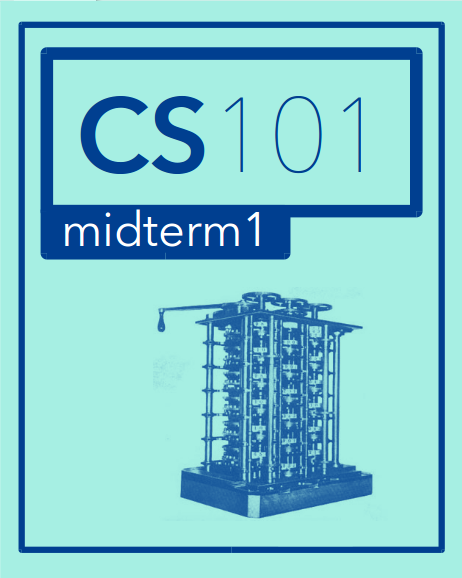
\includegraphics[width=2in]{../img/midterm1-header.png}
\end{center}

\bigskip
\noindent
\begin{itemize}
\item \textbf{Be sure to enter your \underline{NetID} and \underline{the code below} on your Scantron}.
\item Do not turn this page until instructed to do so.
\item There are 30 questions, worth 1 point each.
\item Each question has only \textbf{one} correct answer.
\item You must not communicate with other students during this test.
\item No books, notes, or electronic devices are permitted.
\item This is a 60-minute exam.
\item There are several different versions of this exam.
\end{itemize}

\bigskip\bigskip
\noindent
\textbf{\Large 1. Fill in your information:}

\bigskip
{\Large\bf
\begin{tabular}{ll}
Full Name: & \underbar{\hskip 8cm} \\[0.5em]
UIN (Student Number): & \underbar{\hskip 8cm} \\[0.5em]
NetID: & \underbar{\hskip 8cm}
\end{tabular}
}

\bigskip
\bigskip
\noindent
\textbf{\Large 2. Fill in the following answers on the Scantron form:}

%%%%%%%%%%%%%%%%%%%%%%%%%%%%%%%%%%%%%%%%%%%%%%%%%%%%%%%%%
%%%%%%%%%%%%%%%%%%%%%%%%%%%%%%%%%%%%%%%%%%%%%%%%%%%%%%%%%

\begin{enumerate}
\item[92.] A
\item[93.] A
\item[94.] A
\item[95.] D
\item[96.] C
\end{enumerate}

\newpage

% Zone 1


%%%%%%%%%%%%%%%%%%%%%%%%%%%%%%%%%%%%%%%%%%%%%%%%%%%%%%%%%



\newpage
\noindent
1. (1 point)
Consider the following program:
\begin{verbatim}
s="ECTOR"
t="GAWAIN"
x=len(str(s.isupper()))-t.find("A")
\end{verbatim}
What is the \textbf{type} of \texttt{x} after this program is executed?


\begin{enumerate}
\item[(A)]
\begin{verbatim}Boolean\end{verbatim}

\item[(B)]
\begin{verbatim}String\end{verbatim}

\item[(C)] $\bigstar$ 
\begin{verbatim}Integer\end{verbatim}

\item[(D)]
\begin{verbatim}None\end{verbatim}

\item[(E)]
\begin{verbatim}Float\end{verbatim}

\end{enumerate}

\vspace*{2em}
\hrule
\vspace{2em}

\noindent {\bf Solution.} 
\vspace{2em}
\hrule height 2pt


\newpage
\noindent
2. (1 point)
Consider the following incomplete program.
\begin{verbatim}
sum=0
for i in range(0,100):
    ???

\end{verbatim}
The program is intended to sum all of the integers between 1 and 100 (inclusive). What should replace the three question marks to complete the program?


\begin{enumerate}
\item[(A)]
\begin{verbatim}sum=sum+1\end{verbatim}

\item[(B)] $\bigstar$ 
\begin{verbatim}sum=sum+i+1 \end{verbatim}

\item[(C)]
\begin{verbatim}sum+1=sum \end{verbatim}

\item[(D)]
\begin{verbatim}sum=sum+i \end{verbatim}

\end{enumerate}

\vspace*{2em}
\hrule
\vspace{2em}

\noindent {\bf Solution.} 
\vspace{2em}
\hrule height 2pt


\newpage
\noindent
3. (1 point)
For this problem, you should compose a function which accomplishes a given task using the available code blocks arranged in the correct functional order.  \emph{We ignore indentation for this problem.}

\texttt{find\_max} should accept a \texttt{list} and return the value of the maximum item in the \texttt{list}.  (\texttt{None} is always the lowest value in any numeric comparison, so you may use it as an initializer.)

\begin{verbatim}
def find_max(my_list):
\end{verbatim}

\begin{enumerate}[1]
\item \texttt{max\_val = i}
\item \texttt{max\_val = None}
\item \texttt{for i in range(len(my\_list)):}
\item \texttt{if i > max\_val:}
\item \texttt{max\_val = my\_list[i]}
\item \texttt{return max\_val}
\item \texttt{for i in range(my\_list):}
\item \texttt{if my\_list[i] > max\_val:}
\item \texttt{print(max\_val)}
\end{enumerate}



\begin{enumerate}
\item[(A)]
2, 3, 8, 1, 6

\item[(B)]
2, 7, 4, 5, 6

\item[(C)]
2, 3, 4, 1, 6

\item[(D)] $\bigstar$ 
2, 3, 8, 5, 6

\item[(E)]
3, 2, 8, 5, 9

\end{enumerate}

\vspace*{2em}
\hrule
\vspace{2em}

\noindent {\bf Solution.} 
\vspace{2em}
\hrule height 2pt


\newpage
\noindent
4. (1 point)
How can the following mathematical equation be implemented as a Python expression? Assume \verb|a|, \verb|b|, and \verb|sin| have already been defined.
$$a \sin(a^b - b)$$


\begin{enumerate}
\item[(A)]
None of the other answers are correct.

\item[(B)]
\begin{verbatim}a*sin(a^b - b)\end{verbatim}

\item[(C)]
\begin{verbatim}a sin(a**b - b)\end{verbatim}

\item[(D)] $\bigstar$ 
\begin{verbatim}a*sin(a**b - b)\end{verbatim}

\item[(E)]
\begin{verbatim}a*sin(b^a - b)\end{verbatim}

\end{enumerate}

\vspace*{2em}
\hrule
\vspace{2em}

\noindent {\bf Solution.} 
\vspace{2em}
\hrule height 2pt


\newpage
\noindent
5. (1 point)
Consider the following program:
\begin{verbatim}
x=3
a=5
if (a%3)==2:
    x=x**3
elif(a%3)==1:
    x=x**2
else:
    x=x**1
\end{verbatim}
What is the \textbf{value} of \texttt{x} after this program is executed?


\begin{enumerate}
\item[(A)]
\begin{verbatim}9\end{verbatim}

\item[(B)] $\bigstar$ 
\begin{verbatim}27\end{verbatim}

\item[(C)]
None of the other answers are correct.

\item[(D)]
\begin{verbatim}3\end{verbatim}

\item[(E)]
\begin{verbatim}1\end{verbatim}

\end{enumerate}

\vspace*{2em}
\hrule
\vspace{2em}

\noindent {\bf Solution.} 
\vspace{2em}
\hrule height 2pt


\newpage
\noindent
6. (1 point)
Consider the following program:
\begin{verbatim}
x=0
for i in range(4,10):
    if i%3==0:
        x+=3
    elif i%2==0:
        x+=2
    else:
        x+=1
\end{verbatim}
What is the \textbf{value} of \texttt{x} after this program is executed?


\begin{enumerate}
\item[(A)]
\begin{verbatim}10\end{verbatim}

\item[(B)] $\bigstar$ 
\begin{verbatim}12\end{verbatim}

\item[(C)]
\begin{verbatim}11\end{verbatim}

\item[(D)]
\begin{verbatim}14\end{verbatim}

\item[(E)]
\begin{verbatim}13\end{verbatim}

\end{enumerate}

\vspace*{2em}
\hrule
\vspace{2em}

\noindent {\bf Solution.} 
\vspace{2em}
\hrule height 2pt


\newpage
\noindent
7. (1 point)
Evaluate the following expression:
\begin{verbatim}
[1,2]+[len("3")]
\end{verbatim}
What value is produced?


\begin{enumerate}
\item[(A)] $\bigstar$ 
\begin{verbatim}[1,2,1]\end{verbatim}

\item[(B)]
\begin{verbatim}[1,2,"3"]\end{verbatim}

\item[(C)]
\begin{verbatim}[1,2,1,2,1,2]\end{verbatim}

\item[(D)]
\begin{verbatim}[1,2,3]\end{verbatim}

\end{enumerate}

\vspace*{2em}
\hrule
\vspace{2em}

\noindent {\bf Solution.} 
\vspace{2em}
\hrule height 2pt


\newpage
\noindent
8. (1 point)
Consider the following program.
\begin{verbatim}
kay = 2
wart = 3

def knight(kay,wart):
    wart += 2
    kay += 3
    return wart + kay

wart = knight(kay, kay) + knight(wart, wart)
\end{verbatim}
After it is run, what is the final \textbf{value} of \texttt{wart}?


\begin{enumerate}
\item[(A)]
\begin{verbatim}5\end{verbatim}

\item[(B)] $\bigstar$ 
None of the other answers are correct.

\item[(C)]
\begin{verbatim}2\end{verbatim}

\item[(D)]
\begin{verbatim}3\end{verbatim}

\end{enumerate}

\vspace*{2em}
\hrule
\vspace{2em}

\noindent {\bf Solution.} 
\vspace{2em}
\hrule height 2pt


\newpage
\noindent
9. (1 point)
Consider the following program:
\begin{verbatim}
a=3
b=4
if a==3:
    b=a
elif a==4:
    a=5
else:
    a=b
\end{verbatim}
What is the \textbf{value} of a after this program is executed?


\begin{enumerate}
\item[(A)]
\begin{verbatim}7\end{verbatim}

\item[(B)]
None of the other answers are correct.

\item[(C)]
\begin{verbatim}4\end{verbatim}

\item[(D)] $\bigstar$ 
\begin{verbatim}3\end{verbatim}

\item[(E)]
\begin{verbatim}5\end{verbatim}

\end{enumerate}

\vspace*{2em}
\hrule
\vspace{2em}

\noindent {\bf Solution.} 
\vspace{2em}
\hrule height 2pt


\newpage
\noindent
10. (1 point)
Consider the following program.
\begin{verbatim}
s="ABCBA"
x=0
y=len(s)-1
while s[x]==s[y] and x<=y:
    x+=1
    y-=1
\end{verbatim}
After it is run, what is the final \textbf{value} of \texttt{x}?


\begin{enumerate}
\item[(A)] $\bigstar$ 
\begin{verbatim}3\end{verbatim}

\item[(B)]
\begin{verbatim}0\end{verbatim}

\item[(C)]
\begin{verbatim}1\end{verbatim}

\item[(D)]
\begin{verbatim}4\end{verbatim}

\item[(E)]
\begin{verbatim}2\end{verbatim}

\end{enumerate}

\vspace*{2em}
\hrule
\vspace{2em}

\noindent {\bf Solution.} 
\vspace{2em}
\hrule height 2pt


\newpage
\noindent
11. (1 point)
Consider the following program:
\begin{verbatim}
pi="3.14159"
e="2.71828"
x=pi*len(e)+pi
\end{verbatim}
What is the \textbf{type} of \texttt{x} after this program is executed?


\begin{enumerate}
\item[(A)]
\begin{verbatim}None\end{verbatim}

\item[(B)] $\bigstar$ 
\begin{verbatim}String\end{verbatim}

\item[(C)]
\begin{verbatim}Integer\end{verbatim}

\item[(D)]
\begin{verbatim}Boolean\end{verbatim}

\item[(E)]
\begin{verbatim}Float\end{verbatim}

\end{enumerate}

\vspace*{2em}
\hrule
\vspace{2em}

\noindent {\bf Solution.} 
\vspace{2em}
\hrule height 2pt


\newpage
\noindent
12. (1 point)
Consider the following program:
\begin{verbatim}
x="KING ARTHUR-MORGANA LEFAY-SIR BEDIVERE".split("-")
y=x[:]
y.reverse()
\end{verbatim}
What is the \textbf{value} of \texttt{x} after this program is executed?


\begin{enumerate}
\item[(A)]
\begin{verbatim}['KING', 'ARTHUR-MORGANA', 'LEFAY-SIR', 'BEDIVERE']\end{verbatim}

\item[(B)]
\begin{verbatim}['SIR BEDIVERE', 'MORGANA LEFAY', 'KING ARTHUR']\end{verbatim}

\item[(C)] $\bigstar$ 
\begin{verbatim}['KING ARTHUR', 'MORGANA LEFAY', 'SIR BEDIVERE']\end{verbatim}

\item[(D)]
\begin{verbatim}None\end{verbatim}

\item[(E)]
\begin{verbatim}['BEDIVERE', 'LEFAY-SIR', 'ARTHUR-MORGANA', 'KING']\end{verbatim}

\end{enumerate}

\vspace*{2em}
\hrule
\vspace{2em}

\noindent {\bf Solution.} 
\vspace{2em}
\hrule height 2pt


\newpage
\noindent
13. (1 point)
What is the result of the following expression?
\begin{verbatim}
[ 1, 2, 3 ] * 3.0
\end{verbatim}


\begin{enumerate}
\item[(A)]
\begin{verbatim}[1.0, 2.0, 3.0, 1.0, 2.0, 3.0, 1.0, 2.0, 3.0]\end{verbatim}

\item[(B)] $\bigstar$ 
\begin{verbatim}[1, 2, 3, 1, 2, 3, 1, 2, 3]\end{verbatim}

\item[(C)]
\begin{verbatim}None of the above.\end{verbatim}

\item[(D)]
\begin{verbatim}[3.0, 6.0, 9.0]\end{verbatim}

\item[(E)]
\begin{verbatim}[3, 6, 9]\end{verbatim}

\end{enumerate}

\vspace*{2em}
\hrule
\vspace{2em}

\noindent {\bf Solution.} 
\vspace{2em}
\hrule height 2pt


\newpage
\noindent
14. (1 point)
Consider the following program:
\begin{verbatim}
s="-B-O-R-S-"
x=s.split("-")[2:-2]
\end{verbatim}
What is the \textbf{value} of \texttt{x} after this program is executed?


\begin{enumerate}
\item[(A)]
\begin{verbatim}'ORS'\end{verbatim}

\item[(B)]
\begin{verbatim}''\end{verbatim}

\item[(C)]
\begin{verbatim}False\end{verbatim}

\item[(D)]
\begin{verbatim}None\end{verbatim}

\item[(E)] $\bigstar$ 
\begin{verbatim}['O', 'R']\end{verbatim}

\end{enumerate}

\vspace*{2em}
\hrule
\vspace{2em}

\noindent {\bf Solution.} 
\vspace{2em}
\hrule height 2pt


\newpage
\noindent
15. (1 point)
Consider the following program.
\begin{verbatim}
def artificing(s):
    return s+"%i" % 2
    return s*2
    return s

s=artificing("MERLIN")
\end{verbatim}
After it is run, what is the final \textbf{value} of s?


\begin{enumerate}
\item[(A)]
\begin{verbatim}None\end{verbatim}

\item[(B)]
\begin{verbatim}0\end{verbatim}

\item[(C)]
\begin{verbatim}"MERLINMERLIN"\end{verbatim}

\item[(D)] $\bigstar$ 
\begin{verbatim}"MERLIN2"\end{verbatim}

\item[(E)]
\begin{verbatim}"MERLIN%i"\end{verbatim}

\end{enumerate}

\vspace*{2em}
\hrule
\vspace{2em}

\noindent {\bf Solution.} 
\vspace{2em}
\hrule height 2pt


\newpage
\noindent
16. (1 point)
Consider the following program.
\begin{verbatim}
x=[]
for j in range(0,5):
    if (j%4)==0:
        x.append("-")
    if (j%5)==0:
        x.append("*")
\end{verbatim}
After it is run, what is the final \textbf{value} of \texttt{x}?


\begin{enumerate}
\item[(A)] $\bigstar$ 
\begin{verbatim}["-","*","-"]\end{verbatim}

\item[(B)]
None of the other answers are correct.

\item[(C)]
\begin{verbatim}["-","-","*"]\end{verbatim}

\item[(D)]
\begin{verbatim}["-","*"]\end{verbatim}

\item[(E)]
\begin{verbatim}["-","*","*"]\end{verbatim}

\end{enumerate}

\vspace*{2em}
\hrule
\vspace{2em}

\noindent {\bf Solution.} 
\vspace{2em}
\hrule height 2pt


\newpage
\noindent
17. (1 point)
Consider the following program:
\begin{verbatim}
a=["merlin","sir agravaine","king pellinore"]
b=[ ]
for i in range(0,3):
    b.append(a[0-i].title())
\end{verbatim}
What is the \textbf{value} of b after this program is executed?


\begin{enumerate}
\item[(A)]
\begin{verbatim}[ ]\end{verbatim}

\item[(B)]
\begin{verbatim}['Sir Agravaine', 'King Pellinore']\end{verbatim}

\item[(C)]
\begin{verbatim}['King Pellinore', 'Sir Agravaine']\end{verbatim}

\item[(D)]
\begin{verbatim}['King Pellinore', 'Sir Agravaine', 'Merlin']\end{verbatim}

\item[(E)] $\bigstar$ 
\begin{verbatim}['Merlin', 'King Pellinore', 'Sir Agravaine']\end{verbatim}

\end{enumerate}

\vspace*{2em}
\hrule
\vspace{2em}

\noindent {\bf Solution.} 
\vspace{2em}
\hrule height 2pt


\newpage
\noindent
18. (1 point)
Consider the following program:
\begin{verbatim}
x=[1,2,3]
def f(a):
    s=""
    a.append(4)
    for i in a:
        s+=str(i)
    return s

x.append(f(x))
\end{verbatim}
What is the \textbf{value} of \texttt{x} after this program is executed?


\begin{enumerate}
\item[(A)] $\bigstar$ 
\begin{verbatim}[1, 2, 3, 4, '1234']\end{verbatim}

\item[(B)]
\begin{verbatim}[1, 2, 3, '123']\end{verbatim}

\item[(C)]
\begin{verbatim}[1, 2, 3, 10]\end{verbatim}

\item[(D)]
\begin{verbatim}[1, 2, 3]\end{verbatim}

\item[(E)]
\begin{verbatim}[1, 2, 3, '1234']\end{verbatim}

\end{enumerate}

\vspace*{2em}
\hrule
\vspace{2em}

\noindent {\bf Solution.} 
\vspace{2em}
\hrule height 2pt


\newpage
\noindent
19. (1 point)
Consider the following program:
\begin{verbatim}
a=["S","T","U","P","E","F","Y"]
a=a[0:4]
a.sort()
x=""
for e in a:
    x=e+x
\end{verbatim}
What is the \textbf{value} of \texttt{x} after this program is executed?


\begin{enumerate}
\item[(A)]
None of the other answers are correct.

\item[(B)] $\bigstar$ 
\begin{verbatim}"UTSP"\end{verbatim}

\item[(C)]
\begin{verbatim}"PSTU"\end{verbatim}

\item[(D)]
\begin{verbatim}"STUP"\end{verbatim}

\item[(E)]
\begin{verbatim}"PUST"\end{verbatim}

\end{enumerate}

\vspace*{2em}
\hrule
\vspace{2em}

\noindent {\bf Solution.} 
\vspace{2em}
\hrule height 2pt


\newpage
\noindent
20. (1 point)
Consider the following incomplete Python program.
\begin{verbatim}
s="".join(["2","2","0","1"])
x=0
for i in range(len(s)-1):
    x+=int(???)
\end{verbatim}
What should replace the three question marks so the resulting value of \texttt{x} is 43?


\begin{enumerate}
\item[(A)]
\begin{verbatim}s[i:i-1]\end{verbatim}

\item[(B)]
\begin{verbatim}s[i+1:i+2]\end{verbatim}

\item[(C)]
\begin{verbatim}s[i:i+1]\end{verbatim}

\item[(D)] $\bigstar$ 
\begin{verbatim}s[i:i+2]\end{verbatim}

\end{enumerate}

\vspace*{2em}
\hrule
\vspace{2em}

\noindent {\bf Solution.} 
\vspace{2em}
\hrule height 2pt


\newpage
\noindent
21. (1 point)
\begin{verbatim}
x=str(3)+"str(3)"
\end{verbatim}
What is the \textbf{value} of \texttt{x} after this program is executed?


\begin{enumerate}
\item[(A)] $\bigstar$ 
\begin{verbatim}"3str(3)"\end{verbatim}

\item[(B)]
None of the other answers are correct.

\item[(C)]
\begin{verbatim}"33"\end{verbatim}

\item[(D)]
\begin{verbatim}33\end{verbatim}

\item[(E)]
\begin{verbatim}"333"\end{verbatim}

\end{enumerate}

\vspace*{2em}
\hrule
\vspace{2em}

\noindent {\bf Solution.} 
\vspace{2em}
\hrule height 2pt


\newpage
\noindent
22. (1 point)
Consider the following Python program.
\begin{verbatim}
e=[1,3,5,7,9,11]
d=[0,0,0]
for i in range(0,len(e)):
    d[i%3]+=e[i]
x=d[1]
\end{verbatim}
After it is run, what is the final \textbf{value} of \texttt{x}?


\begin{enumerate}
\item[(A)]
\begin{verbatim}16\end{verbatim}

\item[(B)]
\begin{verbatim}3\end{verbatim}

\item[(C)]
\begin{verbatim}8\end{verbatim}

\item[(D)]
\begin{verbatim}0\end{verbatim}

\item[(E)] $\bigstar$ 
\begin{verbatim}12\end{verbatim}

\end{enumerate}

\vspace*{2em}
\hrule
\vspace{2em}

\noindent {\bf Solution.} 
\vspace{2em}
\hrule height 2pt


\newpage
\noindent
23. (1 point)
Consider the following program:
\begin{verbatim}
x=[1,2,3,4,5,6,7,8,9]
x=x[2:-2]
i=1
while i < 3:
    x[i]+=1
    i+=1
\end{verbatim}
What is the \textbf{value} of \texttt{x} after this program is executed?


\begin{enumerate}
\item[(A)] $\bigstar$ 
\begin{verbatim}[3, 5, 6, 6, 7]\end{verbatim}

\item[(B)]
\begin{verbatim}[3, 5, 6, 6, 7, 8]\end{verbatim}

\item[(C)]
\begin{verbatim}[2, 4, 5, 6, 6, 7]\end{verbatim}

\item[(D)]
\begin{verbatim}[3, 5, 6, 6]\end{verbatim}

\item[(E)]
\begin{verbatim}[2, 4, 5, 5, 6, 7]\end{verbatim}

\end{enumerate}

\vspace*{2em}
\hrule
\vspace{2em}

\noindent {\bf Solution.} 
\vspace{2em}
\hrule height 2pt


\newpage
\noindent
24. (1 point)
Consider the following program:
\begin{verbatim}
i=3
x=2
while i < 7:
    x+=i
    i+=2
\end{verbatim}
What is the \textbf{value} of \texttt{x} after this program is executed?


\begin{enumerate}
\item[(A)]
\begin{verbatim}14\end{verbatim}

\item[(B)]
\begin{verbatim}13\end{verbatim}

\item[(C)]
\begin{verbatim}12\end{verbatim}

\item[(D)] $\bigstar$ 
\begin{verbatim}10\end{verbatim}

\item[(E)]
\begin{verbatim}11\end{verbatim}

\end{enumerate}

\vspace*{2em}
\hrule
\vspace{2em}

\noindent {\bf Solution.} 
\vspace{2em}
\hrule height 2pt


\newpage
\noindent
25. (1 point)
Consider the following program:
\begin{verbatim}
def fix(s):
    a=list(s)
    a.sort()
    return ''.join(a)

x=["one","two","eleven","twelve"]
s1=fix(x[0]+x[-1])
s2=fix(x[1]+x[-2])

if s1<s2:
    x.sort()
elif s1==s2:
    x.reverse()
else:
    x.append("six")
\end{verbatim}
What is the \textbf{value} of \texttt{x} after this program is executed?


\begin{enumerate}
\item[(A)]
\begin{verbatim}['one', 'two', 'eleven', 'twelve']\end{verbatim}

\item[(B)]
\begin{verbatim}['one', 'two', 'eleven', 'twelve', 'six']\end{verbatim}

\item[(C)]
\begin{verbatim}['two', 'twelve', 'one', 'eleven', 'six']\end{verbatim}

\item[(D)] $\bigstar$ 
\begin{verbatim}['twelve', 'eleven', 'two', 'one']\end{verbatim}

\item[(E)]
\begin{verbatim}['eleven', 'one', 'twelve', 'two']\end{verbatim}

\end{enumerate}

\vspace*{2em}
\hrule
\vspace{2em}

\noindent {\bf Solution.} 
\vspace{2em}
\hrule height 2pt


\newpage
\noindent
26. (1 point)
Consider the following incomplete function.
\begin{verbatim}
def ismultiple(m,n):
    if ???:
        return False
    else:
        return True
\end{verbatim}
The function is intended to return True if the input parameter m is a multiple of parameter n and False otherwise. For example, \verb|ismultiple(4,2)| should return \verb|True|, but \verb|ismultiple(5,3)| should return \verb|False|. What should replace the three question marks to complete the function?


\begin{enumerate}
\item[(A)]
\begin{verbatim}(m // n) != 0 \end{verbatim}

\item[(B)]
\begin{verbatim}(n % m) == 0 \end{verbatim}

\item[(C)]
\begin{verbatim}(n // m) == 0 \end{verbatim}

\item[(D)] $\bigstar$ 
\begin{verbatim}(m % n) != 0 \end{verbatim}

\end{enumerate}

\vspace*{2em}
\hrule
\vspace{2em}

\noindent {\bf Solution.} 
\vspace{2em}
\hrule height 2pt


\newpage
\noindent
27. (1 point)
Consider the following program:
\begin{verbatim}
s="Hobbes"
i=0
x=-1
while i<len(s):
    if s[i]=='b':
        x=i
    i+=1
\end{verbatim}
What is the \textbf{value} of \texttt{x} after this program is executed?


\begin{enumerate}
\item[(A)]
\begin{verbatim}5\end{verbatim}

\item[(B)]
\begin{verbatim}4\end{verbatim}

\item[(C)]
\begin{verbatim}2\end{verbatim}

\item[(D)]
\begin{verbatim}-1\end{verbatim}

\item[(E)] $\bigstar$ 
\begin{verbatim}3\end{verbatim}

\end{enumerate}

\vspace*{2em}
\hrule
\vspace{2em}

\noindent {\bf Solution.} 
\vspace{2em}
\hrule height 2pt


\newpage
\noindent
28. (1 point)
Consider the following program.
\begin{verbatim}
x=1
i=0
while(x*x)<=9:
    i=i+(x*x)
    x=x+1
\end{verbatim}
After it is run, what is the final \textbf{value} of \texttt{x}?


\begin{enumerate}
\item[(A)] $\bigstar$ 
\begin{verbatim}4\end{verbatim}

\item[(B)]
\begin{verbatim}5\end{verbatim}

\item[(C)]
\begin{verbatim}14\end{verbatim}

\item[(D)]
\begin{verbatim}3\end{verbatim}

\item[(E)]
\begin{verbatim}30\end{verbatim}

\end{enumerate}

\vspace*{2em}
\hrule
\vspace{2em}

\noindent {\bf Solution.} 
\vspace{2em}
\hrule height 2pt


\newpage
\noindent
29. (1 point)
Consider the following program:
\begin{verbatim}
s="TRIS %i"
t="ISEU"
x=len(s) % len(t[2:-1])
\end{verbatim}
What is the \textbf{type} of \texttt{x} after this program is executed?


\begin{enumerate}
\item[(A)]
\begin{verbatim}Boolean\end{verbatim}

\item[(B)]
\begin{verbatim}None\end{verbatim}

\item[(C)]
\begin{verbatim}Float\end{verbatim}

\item[(D)] $\bigstar$ 
\begin{verbatim}Integer\end{verbatim}

\item[(E)]
\begin{verbatim}String\end{verbatim}

\end{enumerate}

\vspace*{2em}
\hrule
\vspace{2em}

\noindent {\bf Solution.} 
\vspace{2em}
\hrule height 2pt


\newpage
\noindent
30. (1 point)
Evaluate the following expression:
\begin{verbatim}
len("ABCDE"[1:4])
\end{verbatim}
What value is produced?


\begin{enumerate}
\item[(A)]
1

\item[(B)] $\bigstar$ 
3

\item[(C)]
4

\item[(D)]
5

\end{enumerate}

\vspace*{2em}
\hrule
\vspace{2em}

\noindent {\bf Solution.} 
\vspace{2em}
\hrule height 2pt

%%%%%%%%%%%%%%%%%%%%%%%%%%%%%%%%%%%%%%%%%%%%%%%%%%%%%%%%%%%%%%%%%%%%%%
%%%%%%%%%%%%%%%%%%%%%%%%%%%%%%%%%%%%%%%%%%%%%%%%%%%%%%%%%%%%%%%%%%%%%%
%%%%%%%%%%%%%%%%%%%%%%%%%%%%%%%%%%%%%%%%%%%%%%%%%%%%%%%%%%%%%%%%%%%%%%
%%%%%%%%%%%%%%%%%%%%%%%%%%%%%%%%%%%%%%%%%%%%%%%%%%%%%%%%%%%%%%%%%%%%%%
% Exam number 2

\message{Exam 2/50}
\cleardoublepage
\setcounter{page}{1}


\begin{center}
%\textbf{\Large CS 101 Midterm \#1}
%
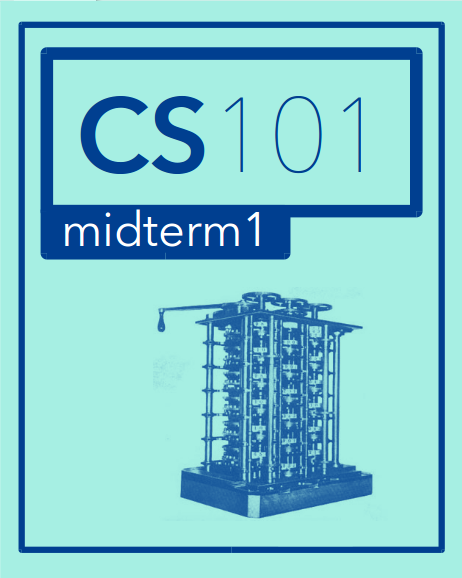
\includegraphics[width=2in]{../img/midterm1-header.png}
\end{center}

\bigskip
\noindent
\begin{itemize}
\item \textbf{Be sure to enter your \underline{NetID} and \underline{the code below} on your Scantron}.
\item Do not turn this page until instructed to do so.
\item There are 30 questions, worth 1 point each.
\item Each question has only \textbf{one} correct answer.
\item You must not communicate with other students during this test.
\item No books, notes, or electronic devices are permitted.
\item This is a 60-minute exam.
\item There are several different versions of this exam.
\end{itemize}

\bigskip\bigskip
\noindent
\textbf{\Large 1. Fill in your information:}

\bigskip
{\Large\bf
\begin{tabular}{ll}
Full Name: & \underbar{\hskip 8cm} \\[0.5em]
UIN (Student Number): & \underbar{\hskip 8cm} \\[0.5em]
NetID: & \underbar{\hskip 8cm}
\end{tabular}
}

\bigskip
\bigskip
\noindent
\textbf{\Large 2. Fill in the following answers on the Scantron form:}

%%%%%%%%%%%%%%%%%%%%%%%%%%%%%%%%%%%%%%%%%%%%%%%%%%%%%%%%%
%%%%%%%%%%%%%%%%%%%%%%%%%%%%%%%%%%%%%%%%%%%%%%%%%%%%%%%%%

\begin{enumerate}
\item[92.] B
\item[93.] A
\item[94.] A
\item[95.] E
\item[96.] D
\end{enumerate}

\newpage

% Zone 1


%%%%%%%%%%%%%%%%%%%%%%%%%%%%%%%%%%%%%%%%%%%%%%%%%%%%%%%%%



\newpage
\noindent
1. (1 point)
Consider the following incomplete program.
\begin{verbatim}
sum=0
for i in range(0,100):
    ???

\end{verbatim}
The program is intended to sum all of the integers between 1 and 100 (inclusive). What should replace the three question marks to complete the program?


\begin{enumerate}
\item[(A)] $\bigstar$ 
\begin{verbatim}sum=sum+i+1 \end{verbatim}

\item[(B)]
\begin{verbatim}sum=sum+i \end{verbatim}

\item[(C)]
\begin{verbatim}sum=sum+1\end{verbatim}

\item[(D)]
\begin{verbatim}sum+1=sum \end{verbatim}

\end{enumerate}

\vspace*{2em}
\hrule
\vspace{2em}

\noindent {\bf Solution.} 
\vspace{2em}
\hrule height 2pt


\newpage
\noindent
2. (1 point)
Consider the following program.
\begin{verbatim}
x=1
i=0
while(x*x)<=9:
    i=i+(x*x)
    x=x+1
\end{verbatim}
After it is run, what is the final \textbf{value} of \texttt{x}?


\begin{enumerate}
\item[(A)]
\begin{verbatim}3\end{verbatim}

\item[(B)]
\begin{verbatim}5\end{verbatim}

\item[(C)] $\bigstar$ 
\begin{verbatim}4\end{verbatim}

\item[(D)]
\begin{verbatim}14\end{verbatim}

\item[(E)]
\begin{verbatim}30\end{verbatim}

\end{enumerate}

\vspace*{2em}
\hrule
\vspace{2em}

\noindent {\bf Solution.} 
\vspace{2em}
\hrule height 2pt


\newpage
\noindent
3. (1 point)
How can the following mathematical equation be implemented as a Python expression? Assume \verb|a|, \verb|b|, and \verb|sin| have already been defined.
$$a \sin(a^b - b)$$


\begin{enumerate}
\item[(A)]
\begin{verbatim}a*sin(a^b - b)\end{verbatim}

\item[(B)]
None of the other answers are correct.

\item[(C)]
\begin{verbatim}a sin(a**b - b)\end{verbatim}

\item[(D)]
\begin{verbatim}a*sin(b^a - b)\end{verbatim}

\item[(E)] $\bigstar$ 
\begin{verbatim}a*sin(a**b - b)\end{verbatim}

\end{enumerate}

\vspace*{2em}
\hrule
\vspace{2em}

\noindent {\bf Solution.} 
\vspace{2em}
\hrule height 2pt


\newpage
\noindent
4. (1 point)
Consider the following program:
\begin{verbatim}
def fix(s):
    a=list(s)
    a.sort()
    return ''.join(a)

x=["one","two","eleven","twelve"]
s1=fix(x[0]+x[-1])
s2=fix(x[1]+x[-2])

if s1<s2:
    x.sort()
elif s1==s2:
    x.reverse()
else:
    x.append("six")
\end{verbatim}
What is the \textbf{value} of \texttt{x} after this program is executed?


\begin{enumerate}
\item[(A)]
\begin{verbatim}['two', 'twelve', 'one', 'eleven', 'six']\end{verbatim}

\item[(B)]
\begin{verbatim}['one', 'two', 'eleven', 'twelve']\end{verbatim}

\item[(C)]
\begin{verbatim}['one', 'two', 'eleven', 'twelve', 'six']\end{verbatim}

\item[(D)] $\bigstar$ 
\begin{verbatim}['twelve', 'eleven', 'two', 'one']\end{verbatim}

\item[(E)]
\begin{verbatim}['eleven', 'one', 'twelve', 'two']\end{verbatim}

\end{enumerate}

\vspace*{2em}
\hrule
\vspace{2em}

\noindent {\bf Solution.} 
\vspace{2em}
\hrule height 2pt


\newpage
\noindent
5. (1 point)
\begin{verbatim}
x=str(3)+"str(3)"
\end{verbatim}
What is the \textbf{value} of \texttt{x} after this program is executed?


\begin{enumerate}
\item[(A)]
\begin{verbatim}"33"\end{verbatim}

\item[(B)]
\begin{verbatim}33\end{verbatim}

\item[(C)] $\bigstar$ 
\begin{verbatim}"3str(3)"\end{verbatim}

\item[(D)]
None of the other answers are correct.

\item[(E)]
\begin{verbatim}"333"\end{verbatim}

\end{enumerate}

\vspace*{2em}
\hrule
\vspace{2em}

\noindent {\bf Solution.} 
\vspace{2em}
\hrule height 2pt


\newpage
\noindent
6. (1 point)
Consider the following program:
\begin{verbatim}
a=3
b=4
if a!=b:
    a=b
elif a==4:
    a=5
else:
    b=a
\end{verbatim}
What is the \textbf{value} of a after this program is executed?


\begin{enumerate}
\item[(A)]
None of the other answers are correct.

\item[(B)]
\begin{verbatim}7\end{verbatim}

\item[(C)]
\begin{verbatim}5\end{verbatim}

\item[(D)]
\begin{verbatim}3\end{verbatim}

\item[(E)] $\bigstar$ 
\begin{verbatim}4\end{verbatim}

\end{enumerate}

\vspace*{2em}
\hrule
\vspace{2em}

\noindent {\bf Solution.} 
\vspace{2em}
\hrule height 2pt


\newpage
\noindent
7. (1 point)
Consider the following program:
\begin{verbatim}
x=0
for i in range(2,7):
    if i%3==0:
        x+=3
    elif i%2==0:
        x+=2
    else:
        x+=1
\end{verbatim}
What is the \textbf{value} of \texttt{x} after this program is executed?


\begin{enumerate}
\item[(A)]
\begin{verbatim}14\end{verbatim}

\item[(B)] $\bigstar$ 
\begin{verbatim}11\end{verbatim}

\item[(C)]
\begin{verbatim}13\end{verbatim}

\item[(D)]
\begin{verbatim}12\end{verbatim}

\item[(E)]
\begin{verbatim}10\end{verbatim}

\end{enumerate}

\vspace*{2em}
\hrule
\vspace{2em}

\noindent {\bf Solution.} 
\vspace{2em}
\hrule height 2pt


\newpage
\noindent
8. (1 point)
Consider the following program.
\begin{verbatim}
def artificing(s):
    return s*2
    return s+"%i" % 2
    return s

s=artificing("MERLIN")
\end{verbatim}
After it is run, what is the final \textbf{value} of s?


\begin{enumerate}
\item[(A)]
\begin{verbatim}12\end{verbatim}

\item[(B)]
\begin{verbatim}"MERLIN"\end{verbatim}

\item[(C)]
\begin{verbatim}None\end{verbatim}

\item[(D)] $\bigstar$ 
\begin{verbatim}"MERLINMERLIN"\end{verbatim}

\item[(E)]
\begin{verbatim}"MERLIN2"\end{verbatim}

\end{enumerate}

\vspace*{2em}
\hrule
\vspace{2em}

\noindent {\bf Solution.} 
\vspace{2em}
\hrule height 2pt


\newpage
\noindent
9. (1 point)
Consider the following program.
\begin{verbatim}
kay = 2
wart = 3

def knight(kay,wart):
    wart += 2
    kay += 3
    return wart + kay

wart = knight(kay, kay) + knight(wart, wart)
\end{verbatim}
After it is run, what is the final \textbf{value} of \texttt{wart}?


\begin{enumerate}
\item[(A)]
\begin{verbatim}3\end{verbatim}

\item[(B)] $\bigstar$ 
None of the other answers are correct.

\item[(C)]
\begin{verbatim}5\end{verbatim}

\item[(D)]
\begin{verbatim}2\end{verbatim}

\end{enumerate}

\vspace*{2em}
\hrule
\vspace{2em}

\noindent {\bf Solution.} 
\vspace{2em}
\hrule height 2pt


\newpage
\noindent
10. (1 point)
Consider the following incomplete function.
\begin{verbatim}
def isdivisible(m,n):
    if ???:
        return False
    else:
        return True
\end{verbatim}
The function is intended to return True if the input parameter m is evenly divisible by the parameter n and False otherwise. For example, \verb|isdivisible(4,2)| should return \verb|True|, but \verb|isdivisible(5,3)| should return \verb|False|. What should replace the three question marks to complete the function?


\begin{enumerate}
\item[(A)]
\begin{verbatim}(n // m) == 0 \end{verbatim}

\item[(B)]
\begin{verbatim}(m // n) != 0 \end{verbatim}

\item[(C)] $\bigstar$ 
\begin{verbatim}(m % n) != 0 \end{verbatim}

\item[(D)]
\begin{verbatim}(n % m) == 0 \end{verbatim}

\end{enumerate}

\vspace*{2em}
\hrule
\vspace{2em}

\noindent {\bf Solution.} 
\vspace{2em}
\hrule height 2pt


\newpage
\noindent
11. (1 point)
Consider the following program:
\begin{verbatim}
s="TRIS %i"
t="ISEU"
x=len(s) % len(t[2:-1])
\end{verbatim}
What is the \textbf{type} of \texttt{x} after this program is executed?


\begin{enumerate}
\item[(A)] $\bigstar$ 
\begin{verbatim}Integer\end{verbatim}

\item[(B)]
\begin{verbatim}None\end{verbatim}

\item[(C)]
\begin{verbatim}Float\end{verbatim}

\item[(D)]
\begin{verbatim}Boolean\end{verbatim}

\item[(E)]
\begin{verbatim}String\end{verbatim}

\end{enumerate}

\vspace*{2em}
\hrule
\vspace{2em}

\noindent {\bf Solution.} 
\vspace{2em}
\hrule height 2pt


\newpage
\noindent
12. (1 point)
Consider the following Python program.
\begin{verbatim}
e=[1,3,5,7,9,11]
d=[0,0,0]
for i in range(0,len(e)):
    d[i%3]+=e[i]
x=d[2]
\end{verbatim}
After it is run, what is the final \textbf{value} of \texttt{x}?


\begin{enumerate}
\item[(A)]
\begin{verbatim}8\end{verbatim}

\item[(B)] $\bigstar$ 
\begin{verbatim}16\end{verbatim}

\item[(C)]
\begin{verbatim}12\end{verbatim}

\item[(D)]
\begin{verbatim}0\end{verbatim}

\item[(E)]
\begin{verbatim}7\end{verbatim}

\end{enumerate}

\vspace*{2em}
\hrule
\vspace{2em}

\noindent {\bf Solution.} 
\vspace{2em}
\hrule height 2pt


\newpage
\noindent
13. (1 point)
What is the result of the following expression?
\begin{verbatim}
[ 1, 2, 3 ] * 3
\end{verbatim}


\begin{enumerate}
\item[(A)] $\bigstar$ 
\begin{verbatim}[1, 2, 3, 1, 2, 3, 1, 2, 3]\end{verbatim}

\item[(B)]
\begin{verbatim}[3, 6, 9]\end{verbatim}

\item[(C)]
\begin{verbatim}(3, 6, 9)\end{verbatim}

\item[(D)]
\begin{verbatim}[1.0, 2.0, 3.0, 1.0, 2.0, 3.0, 1.0, 2.0, 3.0]\end{verbatim}

\item[(E)]
\begin{verbatim}[3.0, 6.0, 9.0]\end{verbatim}

\end{enumerate}

\vspace*{2em}
\hrule
\vspace{2em}

\noindent {\bf Solution.} 
\vspace{2em}
\hrule height 2pt


\newpage
\noindent
14. (1 point)
Consider the following program:
\begin{verbatim}
x=3
a=5
if (a%3)==2:
    x=x**3
elif(a%3)==1:
    x=x**2
else:
    x=x**1
\end{verbatim}
What is the \textbf{value} of \texttt{x} after this program is executed?


\begin{enumerate}
\item[(A)]
None of the other answers are correct.

\item[(B)]
\begin{verbatim}1\end{verbatim}

\item[(C)]
\begin{verbatim}3\end{verbatim}

\item[(D)] $\bigstar$ 
\begin{verbatim}27\end{verbatim}

\item[(E)]
\begin{verbatim}9\end{verbatim}

\end{enumerate}

\vspace*{2em}
\hrule
\vspace{2em}

\noindent {\bf Solution.} 
\vspace{2em}
\hrule height 2pt


\newpage
\noindent
15. (1 point)
Consider the following program:
\begin{verbatim}
a=["merlin","sir agravaine","king pellinore"]
b=[ ]
for i in range(0,3):
    b.append(a[0-i].title())
\end{verbatim}
What is the \textbf{value} of b after this program is executed?


\begin{enumerate}
\item[(A)]
\begin{verbatim}['King Pellinore', 'Sir Agravaine', 'Merlin']\end{verbatim}

\item[(B)]
\begin{verbatim}[ ]\end{verbatim}

\item[(C)]
\begin{verbatim}['King Pellinore', 'Sir Agravaine']\end{verbatim}

\item[(D)] $\bigstar$ 
\begin{verbatim}['Merlin', 'King Pellinore', 'Sir Agravaine']\end{verbatim}

\item[(E)]
\begin{verbatim}['Sir Agravaine', 'King Pellinore']\end{verbatim}

\end{enumerate}

\vspace*{2em}
\hrule
\vspace{2em}

\noindent {\bf Solution.} 
\vspace{2em}
\hrule height 2pt


\newpage
\noindent
16. (1 point)
Consider the following incomplete Python program.
\begin{verbatim}
s="".join(["2","2","0","1"])
x=0
for i in range(len(s)-1):
    x+=int(???)
\end{verbatim}
What should replace the three question marks so the resulting value of \texttt{x} is 43?


\begin{enumerate}
\item[(A)]
\begin{verbatim}s[i+1:i+2]\end{verbatim}

\item[(B)]
\begin{verbatim}s[i:i+1]\end{verbatim}

\item[(C)] $\bigstar$ 
\begin{verbatim}s[i:i+2]\end{verbatim}

\item[(D)]
\begin{verbatim}s[i:i-1]\end{verbatim}

\end{enumerate}

\vspace*{2em}
\hrule
\vspace{2em}

\noindent {\bf Solution.} 
\vspace{2em}
\hrule height 2pt


\newpage
\noindent
17. (1 point)
Consider the following program.
\begin{verbatim}
x=[]
for j in range(0,5):
    if (j%3)==0:
        x.append("-")
    if (j%4)==0:
        x.append("*")
\end{verbatim}
After it is run, what is the final \textbf{value} of \texttt{x}?


\begin{enumerate}
\item[(A)]
\begin{verbatim}["-","*"]\end{verbatim}

\item[(B)]
None of the other answers are correct.

\item[(C)] $\bigstar$ 
\begin{verbatim}["-","*","-","*"]\end{verbatim}

\item[(D)]
\begin{verbatim}["*","-","*"]\end{verbatim}

\item[(E)]
\begin{verbatim}["*","-","*"]\end{verbatim}

\end{enumerate}

\vspace*{2em}
\hrule
\vspace{2em}

\noindent {\bf Solution.} 
\vspace{2em}
\hrule height 2pt


\newpage
\noindent
18. (1 point)
Consider the following program:
\begin{verbatim}
x=[1,2,3,4,5,6,7,8,9]
x=x[2:-2]
i=1
while i < 3:
    x[i]+=1
    i+=1
\end{verbatim}
What is the \textbf{value} of \texttt{x} after this program is executed?


\begin{enumerate}
\item[(A)]
\begin{verbatim}[3, 5, 6, 6]\end{verbatim}

\item[(B)] $\bigstar$ 
\begin{verbatim}[3, 5, 6, 6, 7]\end{verbatim}

\item[(C)]
\begin{verbatim}[3, 5, 6, 6, 7, 8]\end{verbatim}

\item[(D)]
\begin{verbatim}[2, 4, 5, 6, 6, 7]\end{verbatim}

\item[(E)]
\begin{verbatim}[2, 4, 5, 5, 6, 7]\end{verbatim}

\end{enumerate}

\vspace*{2em}
\hrule
\vspace{2em}

\noindent {\bf Solution.} 
\vspace{2em}
\hrule height 2pt


\newpage
\noindent
19. (1 point)
Evaluate the following expression:
\begin{verbatim}
len("ABCD"[0:3])
\end{verbatim}
What value is produced?


\begin{enumerate}
\item[(A)]
4

\item[(B)]
1

\item[(C)]
2

\item[(D)] $\bigstar$ 
3

\end{enumerate}

\vspace*{2em}
\hrule
\vspace{2em}

\noindent {\bf Solution.} 
\vspace{2em}
\hrule height 2pt


\newpage
\noindent
20. (1 point)
For this problem, you should compose a function which accomplishes a given task using the available code blocks arranged in the correct functional order.  \emph{We ignore indentation for this problem.}

\texttt{find\_max} should accept a \texttt{list} and return the value of the maximum item in the \texttt{list}.  (\texttt{None} is always the lowest value in any numeric comparison, so you may use it as an initializer.)

\begin{verbatim}
def find_max(my_list):
\end{verbatim}

\begin{enumerate}[1]
\item \texttt{max\_val = i}
\item \texttt{max\_val = None}
\item \texttt{for i in range(len(my\_list)):}
\item \texttt{if i > max\_val:}
\item \texttt{max\_val = my\_list[i]}
\item \texttt{return max\_val}
\item \texttt{for i in range(my\_list):}
\item \texttt{if my\_list[i] > max\_val:}
\item \texttt{print(max\_val)}
\end{enumerate}



\begin{enumerate}
\item[(A)]
2, 7, 4, 5, 6

\item[(B)]
2, 3, 4, 1, 6

\item[(C)] $\bigstar$ 
2, 3, 8, 5, 6

\item[(D)]
2, 3, 8, 1, 6

\item[(E)]
3, 2, 8, 5, 9

\end{enumerate}

\vspace*{2em}
\hrule
\vspace{2em}

\noindent {\bf Solution.} 
\vspace{2em}
\hrule height 2pt


\newpage
\noindent
21. (1 point)
Evaluate the following expression:
\begin{verbatim}
[1,2]*len("3")
\end{verbatim}
What value is produced?


\begin{enumerate}
\item[(A)]
\begin{verbatim}[1,2,1,2,1,2]\end{verbatim}

\item[(B)]
\begin{verbatim}[1,2,3]\end{verbatim}

\item[(C)] $\bigstar$ 
\begin{verbatim}[1,2]\end{verbatim}

\item[(D)]
\begin{verbatim}[1,2,1]\end{verbatim}

\end{enumerate}

\vspace*{2em}
\hrule
\vspace{2em}

\noindent {\bf Solution.} 
\vspace{2em}
\hrule height 2pt


\newpage
\noindent
22. (1 point)
Consider the following program.
\begin{verbatim}
s="BBCAA"
x=0
y=len(s)-1
while s[x]!=s[y] and x<len(s):
    x+=1
    y-=1
\end{verbatim}
After it is run, what is the final \textbf{value} of \texttt{x}?


\begin{enumerate}
\item[(A)]
\begin{verbatim}0\end{verbatim}

\item[(B)]
\begin{verbatim}1\end{verbatim}

\item[(C)]
\begin{verbatim}3\end{verbatim}

\item[(D)]
\begin{verbatim}4\end{verbatim}

\item[(E)] $\bigstar$ 
\begin{verbatim}2\end{verbatim}

\end{enumerate}

\vspace*{2em}
\hrule
\vspace{2em}

\noindent {\bf Solution.} 
\vspace{2em}
\hrule height 2pt


\newpage
\noindent
23. (1 point)
Consider the following program:
\begin{verbatim}
s="G+R+A+I+L"
x=s.split("+")[1:-2]
\end{verbatim}
What is the \textbf{value} of \texttt{x} after this program is executed?


\begin{enumerate}
\item[(A)] $\bigstar$ 
\begin{verbatim}['R','A']\end{verbatim}

\item[(B)]
\begin{verbatim}None\end{verbatim}

\item[(C)]
\begin{verbatim}'RAI'\end{verbatim}

\item[(D)]
\begin{verbatim}3\end{verbatim}

\item[(E)]
\begin{verbatim}False\end{verbatim}

\end{enumerate}

\vspace*{2em}
\hrule
\vspace{2em}

\noindent {\bf Solution.} 
\vspace{2em}
\hrule height 2pt


\newpage
\noindent
24. (1 point)
Consider the following program:
\begin{verbatim}
a=["A","C","C","I","O"]
a.sort()
a[0]=a[-1]
x=""
for e in a:
    x=x+e
\end{verbatim}
What is the \textbf{value} of \texttt{x} after this program is executed?


\begin{enumerate}
\item[(A)]
\begin{verbatim}"ACCIA"\end{verbatim}

\item[(B)]
None of the other answers are correct.

\item[(C)] $\bigstar$ 
\begin{verbatim}"OCCIO"\end{verbatim}

\item[(D)]
\begin{verbatim}"ICCOI"\end{verbatim}

\item[(E)]
\begin{verbatim}"ACCOA"\end{verbatim}

\end{enumerate}

\vspace*{2em}
\hrule
\vspace{2em}

\noindent {\bf Solution.} 
\vspace{2em}
\hrule height 2pt


\newpage
\noindent
25. (1 point)
Consider the following program:
\begin{verbatim}
pi="3.14159"
e="2.71828"
x=pi*len(e)+pi
\end{verbatim}
What is the \textbf{type} of \texttt{x} after this program is executed?


\begin{enumerate}
\item[(A)]
\begin{verbatim}Boolean\end{verbatim}

\item[(B)]
\begin{verbatim}None\end{verbatim}

\item[(C)]
\begin{verbatim}Integer\end{verbatim}

\item[(D)]
\begin{verbatim}Float\end{verbatim}

\item[(E)] $\bigstar$ 
\begin{verbatim}String\end{verbatim}

\end{enumerate}

\vspace*{2em}
\hrule
\vspace{2em}

\noindent {\bf Solution.} 
\vspace{2em}
\hrule height 2pt


\newpage
\noindent
26. (1 point)
Consider the following program:
\begin{verbatim}
s="Hobbes"
i=0
x=-1
while i<len(s):
    if s[i]=='b':
        x=i
    i+=1
\end{verbatim}
What is the \textbf{value} of \texttt{x} after this program is executed?


\begin{enumerate}
\item[(A)]
\begin{verbatim}5\end{verbatim}

\item[(B)] $\bigstar$ 
\begin{verbatim}3\end{verbatim}

\item[(C)]
\begin{verbatim}2\end{verbatim}

\item[(D)]
\begin{verbatim}-1\end{verbatim}

\item[(E)]
\begin{verbatim}4\end{verbatim}

\end{enumerate}

\vspace*{2em}
\hrule
\vspace{2em}

\noindent {\bf Solution.} 
\vspace{2em}
\hrule height 2pt


\newpage
\noindent
27. (1 point)
Consider the following program:
\begin{verbatim}
s="ECTOR"
t="GAWAIN"
x=(len(s)/(len(t)-1))+1
\end{verbatim}
What is the \textbf{type} of \texttt{x} after this program is executed?


\begin{enumerate}
\item[(A)]
\begin{verbatim}Boolean\end{verbatim}

\item[(B)] $\bigstar$ 
\begin{verbatim}Float\end{verbatim}

\item[(C)]
\begin{verbatim}None\end{verbatim}

\item[(D)]
\begin{verbatim}Integer\end{verbatim}

\item[(E)]
\begin{verbatim}String\end{verbatim}

\end{enumerate}

\vspace*{2em}
\hrule
\vspace{2em}

\noindent {\bf Solution.} 
\vspace{2em}
\hrule height 2pt


\newpage
\noindent
28. (1 point)
Consider the following program:
\begin{verbatim}
x=[1,2,3]
def f(a):
    s=""
    a.reverse()
    for i in a:
        s+=str(i)
    return s

x.append(f(x))
\end{verbatim}
What is the \textbf{value} of \texttt{x} after this program is executed?


\begin{enumerate}
\item[(A)]
\begin{verbatim}[1, 2, 3, '321']\end{verbatim}

\item[(B)] $\bigstar$ 
\begin{verbatim}[3, 2, 1, '321']\end{verbatim}

\item[(C)]
\begin{verbatim}[3, 2, 1]\end{verbatim}

\item[(D)]
\begin{verbatim}[1, 2, 3]\end{verbatim}

\item[(E)]
\begin{verbatim}[1, 2, 3, 6]\end{verbatim}

\end{enumerate}

\vspace*{2em}
\hrule
\vspace{2em}

\noindent {\bf Solution.} 
\vspace{2em}
\hrule height 2pt


\newpage
\noindent
29. (1 point)
Consider the following program:
\begin{verbatim}
i=3
x=2
while i < 7:
    x+=i
    i+=2
\end{verbatim}
What is the \textbf{value} of \texttt{x} after this program is executed?


\begin{enumerate}
\item[(A)] $\bigstar$ 
\begin{verbatim}10\end{verbatim}

\item[(B)]
\begin{verbatim}13\end{verbatim}

\item[(C)]
\begin{verbatim}12\end{verbatim}

\item[(D)]
\begin{verbatim}11\end{verbatim}

\item[(E)]
\begin{verbatim}14\end{verbatim}

\end{enumerate}

\vspace*{2em}
\hrule
\vspace{2em}

\noindent {\bf Solution.} 
\vspace{2em}
\hrule height 2pt


\newpage
\noindent
30. (1 point)
Consider the following program:
\begin{verbatim}
x="KING ARTHUR-MORGANA LEFAY-SIR BEDIVERE".split("-")
y=x
x=y.reverse()
\end{verbatim}
What is the \textbf{value} of \texttt{x} after this program is executed?


\begin{enumerate}
\item[(A)]
\begin{verbatim}['SIR BEDIVERE', 'MORGANA LEFAY', 'KING ARTHUR']\end{verbatim}

\item[(B)]
\begin{verbatim}['KING', 'ARTHUR-MORGANA', 'LEFAY-SIR', 'BEDIVERE']\end{verbatim}

\item[(C)] $\bigstar$ 
\begin{verbatim}None\end{verbatim}

\item[(D)]
\begin{verbatim}['KING ARTHUR', 'MORGANA LEFAY', 'SIR BEDIVERE']\end{verbatim}

\item[(E)]
\begin{verbatim}['BEDIVERE', 'LEFAY-SIR', 'ARTHUR-MORGANA', 'KING']\end{verbatim}

\end{enumerate}

\vspace*{2em}
\hrule
\vspace{2em}

\noindent {\bf Solution.} 
\vspace{2em}
\hrule height 2pt

%%%%%%%%%%%%%%%%%%%%%%%%%%%%%%%%%%%%%%%%%%%%%%%%%%%%%%%%%%%%%%%%%%%%%%
%%%%%%%%%%%%%%%%%%%%%%%%%%%%%%%%%%%%%%%%%%%%%%%%%%%%%%%%%%%%%%%%%%%%%%
%%%%%%%%%%%%%%%%%%%%%%%%%%%%%%%%%%%%%%%%%%%%%%%%%%%%%%%%%%%%%%%%%%%%%%
%%%%%%%%%%%%%%%%%%%%%%%%%%%%%%%%%%%%%%%%%%%%%%%%%%%%%%%%%%%%%%%%%%%%%%
% Exam number 3

\message{Exam 3/50}
\cleardoublepage
\setcounter{page}{1}


\begin{center}
%\textbf{\Large CS 101 Midterm \#1}
%
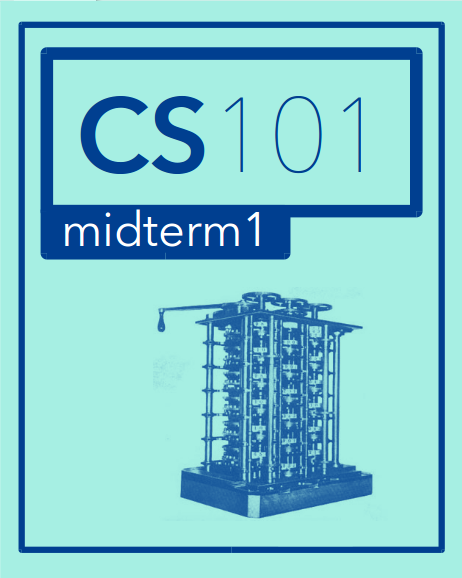
\includegraphics[width=2in]{../img/midterm1-header.png}
\end{center}

\bigskip
\noindent
\begin{itemize}
\item \textbf{Be sure to enter your \underline{NetID} and \underline{the code below} on your Scantron}.
\item Do not turn this page until instructed to do so.
\item There are 30 questions, worth 1 point each.
\item Each question has only \textbf{one} correct answer.
\item You must not communicate with other students during this test.
\item No books, notes, or electronic devices are permitted.
\item This is a 60-minute exam.
\item There are several different versions of this exam.
\end{itemize}

\bigskip\bigskip
\noindent
\textbf{\Large 1. Fill in your information:}

\bigskip
{\Large\bf
\begin{tabular}{ll}
Full Name: & \underbar{\hskip 8cm} \\[0.5em]
UIN (Student Number): & \underbar{\hskip 8cm} \\[0.5em]
NetID: & \underbar{\hskip 8cm}
\end{tabular}
}

\bigskip
\bigskip
\noindent
\textbf{\Large 2. Fill in the following answers on the Scantron form:}

%%%%%%%%%%%%%%%%%%%%%%%%%%%%%%%%%%%%%%%%%%%%%%%%%%%%%%%%%
%%%%%%%%%%%%%%%%%%%%%%%%%%%%%%%%%%%%%%%%%%%%%%%%%%%%%%%%%

\begin{enumerate}
\item[92.] C
\item[93.] A
\item[94.] A
\item[95.] A
\item[96.] E
\end{enumerate}

\newpage

% Zone 1


%%%%%%%%%%%%%%%%%%%%%%%%%%%%%%%%%%%%%%%%%%%%%%%%%%%%%%%%%



\newpage
\noindent
1. (1 point)
Evaluate the following expression:
\begin{verbatim}
len("ABCDE"[1:4])
\end{verbatim}
What value is produced?


\begin{enumerate}
\item[(A)] $\bigstar$ 
3

\item[(B)]
1

\item[(C)]
4

\item[(D)]
5

\end{enumerate}

\vspace*{2em}
\hrule
\vspace{2em}

\noindent {\bf Solution.} 
\vspace{2em}
\hrule height 2pt


\newpage
\noindent
2. (1 point)
Consider the following program.
\begin{verbatim}
s="ABCBA"
x=0
y=len(s)-1
while s[x]==s[y] and x<=y:
    x+=1
    y-=1
\end{verbatim}
After it is run, what is the final \textbf{value} of \texttt{x}?


\begin{enumerate}
\item[(A)]
\begin{verbatim}2\end{verbatim}

\item[(B)] $\bigstar$ 
\begin{verbatim}3\end{verbatim}

\item[(C)]
\begin{verbatim}0\end{verbatim}

\item[(D)]
\begin{verbatim}4\end{verbatim}

\item[(E)]
\begin{verbatim}1\end{verbatim}

\end{enumerate}

\vspace*{2em}
\hrule
\vspace{2em}

\noindent {\bf Solution.} 
\vspace{2em}
\hrule height 2pt


\newpage
\noindent
3. (1 point)
Consider the following program:
\begin{verbatim}
a=3
b=4
if a==3:
    a=b
elif a==4:
    a=5
else:
    b=a
\end{verbatim}
What is the \textbf{value} of a after this program is executed?


\begin{enumerate}
\item[(A)]
\begin{verbatim}5\end{verbatim}

\item[(B)]
\begin{verbatim}3\end{verbatim}

\item[(C)]
\begin{verbatim}7\end{verbatim}

\item[(D)] $\bigstar$ 
\begin{verbatim}4\end{verbatim}

\item[(E)]
None of the other answers are correct.

\end{enumerate}

\vspace*{2em}
\hrule
\vspace{2em}

\noindent {\bf Solution.} 
\vspace{2em}
\hrule height 2pt


\newpage
\noindent
4. (1 point)
Consider the following program:
\begin{verbatim}
a=["S","T","U","P","E","F","Y"]
a=a[0:4]
a.sort()
x=""
for e in a:
    x=e+x
\end{verbatim}
What is the \textbf{value} of \texttt{x} after this program is executed?


\begin{enumerate}
\item[(A)] $\bigstar$ 
\begin{verbatim}"UTSP"\end{verbatim}

\item[(B)]
None of the other answers are correct.

\item[(C)]
\begin{verbatim}"PUST"\end{verbatim}

\item[(D)]
\begin{verbatim}"STUP"\end{verbatim}

\item[(E)]
\begin{verbatim}"PSTU"\end{verbatim}

\end{enumerate}

\vspace*{2em}
\hrule
\vspace{2em}

\noindent {\bf Solution.} 
\vspace{2em}
\hrule height 2pt


\newpage
\noindent
5. (1 point)
Consider the following program:
\begin{verbatim}
x=[1,2,3,4,5,6,7,8,9]
x=x[2:-2]
i=1
while i <= 3:
    x[i]+=1
    i+=1
\end{verbatim}
What is the \textbf{value} of \texttt{x} after this program is executed?


\begin{enumerate}
\item[(A)]
\begin{verbatim}[2, 4, 5, 6, 7, 7]\end{verbatim}

\item[(B)]
\begin{verbatim}[3, 5, 7, 7]\end{verbatim}

\item[(C)] $\bigstar$ 
\begin{verbatim}[3, 5, 6, 7, 7]\end{verbatim}

\item[(D)]
\begin{verbatim}[3, 5, 6, 7, 7, 8]\end{verbatim}

\item[(E)]
\begin{verbatim}[2, 4, 5, 5, 7, 7]\end{verbatim}

\end{enumerate}

\vspace*{2em}
\hrule
\vspace{2em}

\noindent {\bf Solution.} 
\vspace{2em}
\hrule height 2pt


\newpage
\noindent
6. (1 point)
Consider the following Python program.
\begin{verbatim}
e=[1,3,5,7,9,11]
d=[0,0,0]
for i in range(0,len(e)):
    d[i%3]+=e[i]
x=d[1]
\end{verbatim}
After it is run, what is the final \textbf{value} of \texttt{x}?


\begin{enumerate}
\item[(A)]
\begin{verbatim}0\end{verbatim}

\item[(B)] $\bigstar$ 
\begin{verbatim}12\end{verbatim}

\item[(C)]
\begin{verbatim}8\end{verbatim}

\item[(D)]
\begin{verbatim}16\end{verbatim}

\item[(E)]
\begin{verbatim}3\end{verbatim}

\end{enumerate}

\vspace*{2em}
\hrule
\vspace{2em}

\noindent {\bf Solution.} 
\vspace{2em}
\hrule height 2pt


\newpage
\noindent
7. (1 point)
Consider the following program.
\begin{verbatim}
x=0
i=1
while(i*i)<=9:
    x=x+(i*i)
    i=i+1
\end{verbatim}
After it is run, what is the final \textbf{value} of \texttt{x}?


\begin{enumerate}
\item[(A)]
\begin{verbatim}5\end{verbatim}

\item[(B)] $\bigstar$ 
\begin{verbatim}14\end{verbatim}

\item[(C)]
\begin{verbatim}3\end{verbatim}

\item[(D)]
\begin{verbatim}4\end{verbatim}

\item[(E)]
\begin{verbatim}30\end{verbatim}

\end{enumerate}

\vspace*{2em}
\hrule
\vspace{2em}

\noindent {\bf Solution.} 
\vspace{2em}
\hrule height 2pt


\newpage
\noindent
8. (1 point)
Consider the following program:
\begin{verbatim}
a=["merlin","sir agravaine","king pellinore"]
b=[ ]
for i in range(0,3):
    b.append(a[0-i].title())
\end{verbatim}
What is the \textbf{value} of b after this program is executed?


\begin{enumerate}
\item[(A)]
\begin{verbatim}['Sir Agravaine', 'King Pellinore']\end{verbatim}

\item[(B)]
\begin{verbatim}['King Pellinore', 'Sir Agravaine']\end{verbatim}

\item[(C)] $\bigstar$ 
\begin{verbatim}['Merlin', 'King Pellinore', 'Sir Agravaine']\end{verbatim}

\item[(D)]
\begin{verbatim}[ ]\end{verbatim}

\item[(E)]
\begin{verbatim}['King Pellinore', 'Sir Agravaine', 'Merlin']\end{verbatim}

\end{enumerate}

\vspace*{2em}
\hrule
\vspace{2em}

\noindent {\bf Solution.} 
\vspace{2em}
\hrule height 2pt


\newpage
\noindent
9. (1 point)
Consider the following program:
\begin{verbatim}
x="KING ARTHUR-MORGANA LEFAY-SIR BEDIVERE".split("-")
y=x
x=y.reverse()
\end{verbatim}
What is the \textbf{value} of \texttt{x} after this program is executed?


\begin{enumerate}
\item[(A)]
\begin{verbatim}['SIR BEDIVERE', 'MORGANA LEFAY', 'KING ARTHUR']\end{verbatim}

\item[(B)]
\begin{verbatim}['KING', 'ARTHUR-MORGANA', 'LEFAY-SIR', 'BEDIVERE']\end{verbatim}

\item[(C)]
\begin{verbatim}['KING ARTHUR', 'MORGANA LEFAY', 'SIR BEDIVERE']\end{verbatim}

\item[(D)]
\begin{verbatim}['BEDIVERE', 'LEFAY-SIR', 'ARTHUR-MORGANA', 'KING']\end{verbatim}

\item[(E)] $\bigstar$ 
\begin{verbatim}None\end{verbatim}

\end{enumerate}

\vspace*{2em}
\hrule
\vspace{2em}

\noindent {\bf Solution.} 
\vspace{2em}
\hrule height 2pt


\newpage
\noindent
10. (1 point)
Consider the following program:
\begin{verbatim}
x=[1,2,3]
def f(a):
    s=""
    a.reverse()
    for i in a:
        s+=str(i)
    return s

x.append(f(x))
\end{verbatim}
What is the \textbf{value} of \texttt{x} after this program is executed?


\begin{enumerate}
\item[(A)]
\begin{verbatim}[1, 2, 3, 6]\end{verbatim}

\item[(B)]
\begin{verbatim}[1, 2, 3, '321']\end{verbatim}

\item[(C)]
\begin{verbatim}[1, 2, 3]\end{verbatim}

\item[(D)]
\begin{verbatim}[3, 2, 1]\end{verbatim}

\item[(E)] $\bigstar$ 
\begin{verbatim}[3, 2, 1, '321']\end{verbatim}

\end{enumerate}

\vspace*{2em}
\hrule
\vspace{2em}

\noindent {\bf Solution.} 
\vspace{2em}
\hrule height 2pt


\newpage
\noindent
11. (1 point)
Consider the following program.
\begin{verbatim}
kay = 2
wart = 3

def knight(kay,wart):
    wart += 2
    kay += 3
    return wart + kay

wart = knight(kay, kay) + knight(wart, wart)
\end{verbatim}
After it is run, what is the final \textbf{value} of \texttt{wart}?


\begin{enumerate}
\item[(A)]
\begin{verbatim}2\end{verbatim}

\item[(B)]
\begin{verbatim}3\end{verbatim}

\item[(C)]
\begin{verbatim}5\end{verbatim}

\item[(D)] $\bigstar$ 
None of the other answers are correct.

\end{enumerate}

\vspace*{2em}
\hrule
\vspace{2em}

\noindent {\bf Solution.} 
\vspace{2em}
\hrule height 2pt


\newpage
\noindent
12. (1 point)
Consider the following program:
\begin{verbatim}
s="TRIS %i"
t="ISEU"
x=len(s) % len(t[2:-1])
\end{verbatim}
What is the \textbf{type} of \texttt{x} after this program is executed?


\begin{enumerate}
\item[(A)] $\bigstar$ 
\begin{verbatim}Integer\end{verbatim}

\item[(B)]
\begin{verbatim}Float\end{verbatim}

\item[(C)]
\begin{verbatim}None\end{verbatim}

\item[(D)]
\begin{verbatim}String\end{verbatim}

\item[(E)]
\begin{verbatim}Boolean\end{verbatim}

\end{enumerate}

\vspace*{2em}
\hrule
\vspace{2em}

\noindent {\bf Solution.} 
\vspace{2em}
\hrule height 2pt


\newpage
\noindent
13. (1 point)
Consider the following program:
\begin{verbatim}
x=str("1"*3)
\end{verbatim}
What is the \textbf{value} of \texttt{x} after this program is executed?


\begin{enumerate}
\item[(A)]
\begin{verbatim}"3"\end{verbatim}

\item[(B)]
None of the other answers are correct.

\item[(C)]
\begin{verbatim}111\end{verbatim}

\item[(D)] $\bigstar$ 
\begin{verbatim}"111"\end{verbatim}

\item[(E)]
\begin{verbatim}3\end{verbatim}

\end{enumerate}

\vspace*{2em}
\hrule
\vspace{2em}

\noindent {\bf Solution.} 
\vspace{2em}
\hrule height 2pt


\newpage
\noindent
14. (1 point)
Consider the following incomplete function.
\begin{verbatim}
def ismultiple(m,n):
    if ???:
        return False
    else:
        return True
\end{verbatim}
The function is intended to return True if the input parameter m is a multiple of parameter n and False otherwise. For example, \verb|ismultiple(4,2)| should return \verb|True|, but \verb|ismultiple(5,3)| should return \verb|False|. What should replace the three question marks to complete the function?


\begin{enumerate}
\item[(A)] $\bigstar$ 
\begin{verbatim}(m % n) != 0 \end{verbatim}

\item[(B)]
\begin{verbatim}(m // n) != 0 \end{verbatim}

\item[(C)]
\begin{verbatim}(n % m) == 0 \end{verbatim}

\item[(D)]
\begin{verbatim}(n // m) == 0 \end{verbatim}

\end{enumerate}

\vspace*{2em}
\hrule
\vspace{2em}

\noindent {\bf Solution.} 
\vspace{2em}
\hrule height 2pt


\newpage
\noindent
15. (1 point)
Consider the following incomplete program.
\begin{verbatim}
sum=0
for i in range(0,100):
    ???

\end{verbatim}
The program is intended to sum all of the integers between 1 and 100 (inclusive). What should replace the three question marks to complete the program?


\begin{enumerate}
\item[(A)]
\begin{verbatim}sum=sum+1\end{verbatim}

\item[(B)] $\bigstar$ 
\begin{verbatim}sum=sum+i+1 \end{verbatim}

\item[(C)]
\begin{verbatim}sum=sum+i \end{verbatim}

\item[(D)]
\begin{verbatim}sum+1=sum \end{verbatim}

\end{enumerate}

\vspace*{2em}
\hrule
\vspace{2em}

\noindent {\bf Solution.} 
\vspace{2em}
\hrule height 2pt


\newpage
\noindent
16. (1 point)
What is the result of the following expression?
\begin{verbatim}
[ 1, 2, 3 ] * 3.0
\end{verbatim}


\begin{enumerate}
\item[(A)]
\begin{verbatim}None of the above.\end{verbatim}

\item[(B)]
\begin{verbatim}[3.0, 6.0, 9.0]\end{verbatim}

\item[(C)]
\begin{verbatim}[1.0, 2.0, 3.0, 1.0, 2.0, 3.0, 1.0, 2.0, 3.0]\end{verbatim}

\item[(D)] $\bigstar$ 
\begin{verbatim}[1, 2, 3, 1, 2, 3, 1, 2, 3]\end{verbatim}

\item[(E)]
\begin{verbatim}[3, 6, 9]\end{verbatim}

\end{enumerate}

\vspace*{2em}
\hrule
\vspace{2em}

\noindent {\bf Solution.} 
\vspace{2em}
\hrule height 2pt


\newpage
\noindent
17. (1 point)
Consider the following program.
\begin{verbatim}
x=[]
for j in range(0,5):
    if (j%4)==0:
        x.append("-")
    if (j%5)==0:
        x.append("*")
\end{verbatim}
After it is run, what is the final \textbf{value} of \texttt{x}?


\begin{enumerate}
\item[(A)]
\begin{verbatim}["-","*","*"]\end{verbatim}

\item[(B)]
\begin{verbatim}["-","-","*"]\end{verbatim}

\item[(C)]
\begin{verbatim}["-","*"]\end{verbatim}

\item[(D)]
None of the other answers are correct.

\item[(E)] $\bigstar$ 
\begin{verbatim}["-","*","-"]\end{verbatim}

\end{enumerate}

\vspace*{2em}
\hrule
\vspace{2em}

\noindent {\bf Solution.} 
\vspace{2em}
\hrule height 2pt


\newpage
\noindent
18. (1 point)
Consider the following program:
\begin{verbatim}
s="Calvin"
i=0
x=-1
while i<len(s):
    if s[i]=='b':
        x=i
    i+=1
\end{verbatim}
What is the \textbf{value} of \texttt{x} after this program is executed?


\begin{enumerate}
\item[(A)]
\begin{verbatim}6\end{verbatim}

\item[(B)] $\bigstar$ 
\begin{verbatim}-1\end{verbatim}

\item[(C)]
\begin{verbatim}5\end{verbatim}

\item[(D)]
\begin{verbatim}3\end{verbatim}

\item[(E)]
\begin{verbatim}0\end{verbatim}

\end{enumerate}

\vspace*{2em}
\hrule
\vspace{2em}

\noindent {\bf Solution.} 
\vspace{2em}
\hrule height 2pt


\newpage
\noindent
19. (1 point)
Consider the following program:
\begin{verbatim}
i=3
x=2
while i < 7:
    x+=i
    i+=2
\end{verbatim}
What is the \textbf{value} of \texttt{x} after this program is executed?


\begin{enumerate}
\item[(A)]
\begin{verbatim}13\end{verbatim}

\item[(B)] $\bigstar$ 
\begin{verbatim}10\end{verbatim}

\item[(C)]
\begin{verbatim}11\end{verbatim}

\item[(D)]
\begin{verbatim}12\end{verbatim}

\item[(E)]
\begin{verbatim}14\end{verbatim}

\end{enumerate}

\vspace*{2em}
\hrule
\vspace{2em}

\noindent {\bf Solution.} 
\vspace{2em}
\hrule height 2pt


\newpage
\noindent
20. (1 point)
Consider the following program:
\begin{verbatim}
x=3
a=7
if (a%3)==2:
    x=x**2
elif(a%3)==1:
    x=x**1
else:
    x=x**0
\end{verbatim}
What is the \textbf{value} of \texttt{x} after this program is executed?


\begin{enumerate}
\item[(A)] $\bigstar$ 
\begin{verbatim}3\end{verbatim}

\item[(B)]
\begin{verbatim}9\end{verbatim}

\item[(C)]
None of the other answers are correct.

\item[(D)]
\begin{verbatim}1\end{verbatim}

\item[(E)]
\begin{verbatim}7\end{verbatim}

\end{enumerate}

\vspace*{2em}
\hrule
\vspace{2em}

\noindent {\bf Solution.} 
\vspace{2em}
\hrule height 2pt


\newpage
\noindent
21. (1 point)
Consider the following program:
\begin{verbatim}
def fix(s):
    a=list(s)
    a.sort()
    return ''.join(a)

x=["one","two","eleven","twelve"]
s1=fix(x[0]+x[-1])
s2=fix(x[1]+x[-2])

if s1==s2:
    x.sort()
elif s1<s2:
    x.reverse()
else:
    x.append("six")
\end{verbatim}
What is the \textbf{value} of \texttt{x} after this program is executed?


\begin{enumerate}
\item[(A)] $\bigstar$ 
\begin{verbatim}['eleven', 'one', 'twelve', 'two']\end{verbatim}

\item[(B)]
\begin{verbatim}['one', 'two', 'eleven', 'twelve']\end{verbatim}

\item[(C)]
\begin{verbatim}['one', 'two', 'eleven', 'twelve', 'six']\end{verbatim}

\item[(D)]
\begin{verbatim}['two', 'twelve', 'one', 'eleven', 'six']\end{verbatim}

\item[(E)]
\begin{verbatim}['twelve', 'eleven', 'two', 'one']\end{verbatim}

\end{enumerate}

\vspace*{2em}
\hrule
\vspace{2em}

\noindent {\bf Solution.} 
\vspace{2em}
\hrule height 2pt


\newpage
\noindent
22. (1 point)
Evaluate the following expression:
\begin{verbatim}
[1,2]*len("3")
\end{verbatim}
What value is produced?


\begin{enumerate}
\item[(A)]
\begin{verbatim}[1,2,3]\end{verbatim}

\item[(B)]
\begin{verbatim}[1,2,1]\end{verbatim}

\item[(C)] $\bigstar$ 
\begin{verbatim}[1,2]\end{verbatim}

\item[(D)]
\begin{verbatim}[1,2,1,2,1,2]\end{verbatim}

\end{enumerate}

\vspace*{2em}
\hrule
\vspace{2em}

\noindent {\bf Solution.} 
\vspace{2em}
\hrule height 2pt


\newpage
\noindent
23. (1 point)
Consider the following incomplete Python program.
\begin{verbatim}
s="".join(["0","1","2","1"])
x=0
for i in range(len(s)-1):
    x+=int(???)
\end{verbatim}
What should replace the three question marks so the resulting value of \texttt{x} is 34?


\begin{enumerate}
\item[(A)]
\begin{verbatim}s[i:i-1]\end{verbatim}

\item[(B)]
\begin{verbatim}s[i+1:i+2]\end{verbatim}

\item[(C)] $\bigstar$ 
\begin{verbatim}s[i:i+2]\end{verbatim}

\item[(D)]
\begin{verbatim}s[i:i+1]\end{verbatim}

\end{enumerate}

\vspace*{2em}
\hrule
\vspace{2em}

\noindent {\bf Solution.} 
\vspace{2em}
\hrule height 2pt


\newpage
\noindent
24. (1 point)
Consider the following program:
\begin{verbatim}
s="ECTOR"
t="GAWAIN"
x=(len(s)+len(t)) < 4 and s in t
\end{verbatim}
What is the \textbf{type} of \texttt{x} after this program is executed?


\begin{enumerate}
\item[(A)]
\begin{verbatim}Integer\end{verbatim}

\item[(B)]
\begin{verbatim}Float\end{verbatim}

\item[(C)]
\begin{verbatim}None\end{verbatim}

\item[(D)] $\bigstar$ 
\begin{verbatim}Boolean\end{verbatim}

\item[(E)]
\begin{verbatim}String\end{verbatim}

\end{enumerate}

\vspace*{2em}
\hrule
\vspace{2em}

\noindent {\bf Solution.} 
\vspace{2em}
\hrule height 2pt


\newpage
\noindent
25. (1 point)
Consider the following program:
\begin{verbatim}
pi="3.14159"
e="2.71828"
x=(float(e)**float(pi)-float(pi)) == 20
\end{verbatim}
What is the \textbf{type} of \texttt{x} after this program is executed?


\begin{enumerate}
\item[(A)]
\begin{verbatim}None\end{verbatim}

\item[(B)]
\begin{verbatim}Integer\end{verbatim}

\item[(C)]
\begin{verbatim}Float\end{verbatim}

\item[(D)] $\bigstar$ 
\begin{verbatim}Boolean\end{verbatim}

\item[(E)]
\begin{verbatim}String\end{verbatim}

\end{enumerate}

\vspace*{2em}
\hrule
\vspace{2em}

\noindent {\bf Solution.} 
\vspace{2em}
\hrule height 2pt


\newpage
\noindent
26. (1 point)
Consider the following program.
\begin{verbatim}
def artificing(s):
    return s*2
    return s+"%i" % 2
    return s

s=artificing("MERLIN")
\end{verbatim}
After it is run, what is the final \textbf{value} of s?


\begin{enumerate}
\item[(A)]
\begin{verbatim}12\end{verbatim}

\item[(B)]
\begin{verbatim}"MERLIN2"\end{verbatim}

\item[(C)]
\begin{verbatim}"MERLIN"\end{verbatim}

\item[(D)]
\begin{verbatim}None\end{verbatim}

\item[(E)] $\bigstar$ 
\begin{verbatim}"MERLINMERLIN"\end{verbatim}

\end{enumerate}

\vspace*{2em}
\hrule
\vspace{2em}

\noindent {\bf Solution.} 
\vspace{2em}
\hrule height 2pt


\newpage
\noindent
27. (1 point)
Consider the following program:
\begin{verbatim}
s="-B-O-R-S-"
x=s.split("-")[2:-2]
\end{verbatim}
What is the \textbf{value} of \texttt{x} after this program is executed?


\begin{enumerate}
\item[(A)]
\begin{verbatim}None\end{verbatim}

\item[(B)] $\bigstar$ 
\begin{verbatim}['O', 'R']\end{verbatim}

\item[(C)]
\begin{verbatim}False\end{verbatim}

\item[(D)]
\begin{verbatim}'ORS'\end{verbatim}

\item[(E)]
\begin{verbatim}''\end{verbatim}

\end{enumerate}

\vspace*{2em}
\hrule
\vspace{2em}

\noindent {\bf Solution.} 
\vspace{2em}
\hrule height 2pt


\newpage
\noindent
28. (1 point)
Consider the following program:
\begin{verbatim}
x=0
for i in range(2,8):
    if i%3==0:
        x+=3
    elif i%2==0:
        x+=2
    else:
        x+=1
\end{verbatim}
What is the \textbf{value} of \texttt{x} after this program is executed?


\begin{enumerate}
\item[(A)] $\bigstar$ 
\begin{verbatim}12\end{verbatim}

\item[(B)]
\begin{verbatim}14\end{verbatim}

\item[(C)]
\begin{verbatim}10\end{verbatim}

\item[(D)]
\begin{verbatim}13\end{verbatim}

\item[(E)]
\begin{verbatim}11\end{verbatim}

\end{enumerate}

\vspace*{2em}
\hrule
\vspace{2em}

\noindent {\bf Solution.} 
\vspace{2em}
\hrule height 2pt


\newpage
\noindent
29. (1 point)
For this problem, you should compose a function which accomplishes a given task using the available code blocks arranged in the correct functional order.  \emph{We ignore indentation for this problem.}

\texttt{find\_max} should accept a \texttt{list} and return the value of the maximum item in the \texttt{list}.  (\texttt{None} is always the lowest value in any numeric comparison, so you may use it as an initializer.)

\begin{verbatim}
def find_max(my_list):
\end{verbatim}

\begin{enumerate}[1]
\item \texttt{max\_val = i}
\item \texttt{max\_val = None}
\item \texttt{for i in range(len(my\_list)):}
\item \texttt{if i > max\_val:}
\item \texttt{max\_val = my\_list[i]}
\item \texttt{return max\_val}
\item \texttt{for i in range(my\_list):}
\item \texttt{if my\_list[i] > max\_val:}
\item \texttt{print(max\_val)}
\end{enumerate}



\begin{enumerate}
\item[(A)] $\bigstar$ 
2, 3, 8, 5, 6

\item[(B)]
3, 2, 8, 5, 9

\item[(C)]
2, 3, 4, 1, 6

\item[(D)]
2, 3, 8, 1, 6

\item[(E)]
2, 7, 4, 5, 6

\end{enumerate}

\vspace*{2em}
\hrule
\vspace{2em}

\noindent {\bf Solution.} 
\vspace{2em}
\hrule height 2pt


\newpage
\noindent
30. (1 point)
How can the following mathematical equation be implemented as a Python expression? Assume \verb|a|, \verb|b|, and \verb|sin| have already been defined.
$$a \sin(a^b - b)$$


\begin{enumerate}
\item[(A)]
\begin{verbatim}a*sin(a^b - b)\end{verbatim}

\item[(B)]
\begin{verbatim}a*sin(b^a - b)\end{verbatim}

\item[(C)]
\begin{verbatim}a sin(a**b - b)\end{verbatim}

\item[(D)] $\bigstar$ 
\begin{verbatim}a*sin(a**b - b)\end{verbatim}

\item[(E)]
None of the other answers are correct.

\end{enumerate}

\vspace*{2em}
\hrule
\vspace{2em}

\noindent {\bf Solution.} 
\vspace{2em}
\hrule height 2pt

%%%%%%%%%%%%%%%%%%%%%%%%%%%%%%%%%%%%%%%%%%%%%%%%%%%%%%%%%%%%%%%%%%%%%%
%%%%%%%%%%%%%%%%%%%%%%%%%%%%%%%%%%%%%%%%%%%%%%%%%%%%%%%%%%%%%%%%%%%%%%
%%%%%%%%%%%%%%%%%%%%%%%%%%%%%%%%%%%%%%%%%%%%%%%%%%%%%%%%%%%%%%%%%%%%%%
%%%%%%%%%%%%%%%%%%%%%%%%%%%%%%%%%%%%%%%%%%%%%%%%%%%%%%%%%%%%%%%%%%%%%%
% Exam number 4

\message{Exam 4/50}
\cleardoublepage
\setcounter{page}{1}


\begin{center}
%\textbf{\Large CS 101 Midterm \#1}
%
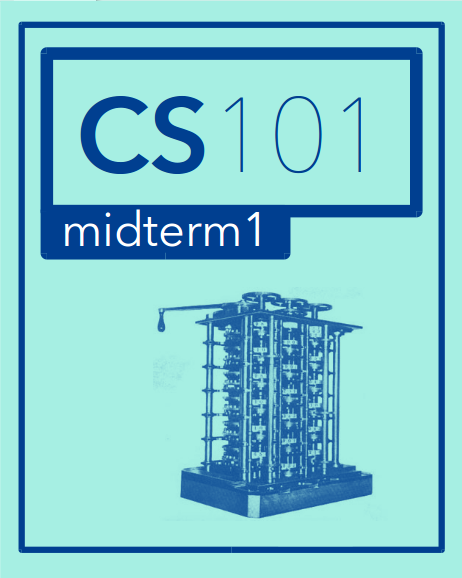
\includegraphics[width=2in]{../img/midterm1-header.png}
\end{center}

\bigskip
\noindent
\begin{itemize}
\item \textbf{Be sure to enter your \underline{NetID} and \underline{the code below} on your Scantron}.
\item Do not turn this page until instructed to do so.
\item There are 30 questions, worth 1 point each.
\item Each question has only \textbf{one} correct answer.
\item You must not communicate with other students during this test.
\item No books, notes, or electronic devices are permitted.
\item This is a 60-minute exam.
\item There are several different versions of this exam.
\end{itemize}

\bigskip\bigskip
\noindent
\textbf{\Large 1. Fill in your information:}

\bigskip
{\Large\bf
\begin{tabular}{ll}
Full Name: & \underbar{\hskip 8cm} \\[0.5em]
UIN (Student Number): & \underbar{\hskip 8cm} \\[0.5em]
NetID: & \underbar{\hskip 8cm}
\end{tabular}
}

\bigskip
\bigskip
\noindent
\textbf{\Large 2. Fill in the following answers on the Scantron form:}

%%%%%%%%%%%%%%%%%%%%%%%%%%%%%%%%%%%%%%%%%%%%%%%%%%%%%%%%%
%%%%%%%%%%%%%%%%%%%%%%%%%%%%%%%%%%%%%%%%%%%%%%%%%%%%%%%%%

\begin{enumerate}
\item[92.] D
\item[93.] A
\item[94.] A
\item[95.] B
\item[96.] A
\end{enumerate}

\newpage

% Zone 1


%%%%%%%%%%%%%%%%%%%%%%%%%%%%%%%%%%%%%%%%%%%%%%%%%%%%%%%%%



\newpage
\noindent
1. (1 point)
What is the result of the following expression?
\begin{verbatim}
[ 1, 2, 3 ] * 3
\end{verbatim}


\begin{enumerate}
\item[(A)]
\begin{verbatim}[3, 6, 9]\end{verbatim}

\item[(B)] $\bigstar$ 
\begin{verbatim}[1, 2, 3, 1, 2, 3, 1, 2, 3]\end{verbatim}

\item[(C)]
\begin{verbatim}[3.0, 6.0, 9.0]\end{verbatim}

\item[(D)]
\begin{verbatim}[1.0, 2.0, 3.0, 1.0, 2.0, 3.0, 1.0, 2.0, 3.0]\end{verbatim}

\item[(E)]
\begin{verbatim}(3, 6, 9)\end{verbatim}

\end{enumerate}

\vspace*{2em}
\hrule
\vspace{2em}

\noindent {\bf Solution.} 
\vspace{2em}
\hrule height 2pt


\newpage
\noindent
2. (1 point)
Consider the following program:
\begin{verbatim}
x=3
a=5
if (a%3)==2:
    x=x**3
elif(a%3)==1:
    x=x**2
else:
    x=x**1
\end{verbatim}
What is the \textbf{value} of \texttt{x} after this program is executed?


\begin{enumerate}
\item[(A)]
\begin{verbatim}3\end{verbatim}

\item[(B)] $\bigstar$ 
\begin{verbatim}27\end{verbatim}

\item[(C)]
None of the other answers are correct.

\item[(D)]
\begin{verbatim}9\end{verbatim}

\item[(E)]
\begin{verbatim}1\end{verbatim}

\end{enumerate}

\vspace*{2em}
\hrule
\vspace{2em}

\noindent {\bf Solution.} 
\vspace{2em}
\hrule height 2pt


\newpage
\noindent
3. (1 point)
Consider the following program:
\begin{verbatim}
s="TRIS %i"
t="ISEU"
x=len(s) % len(t[2:-1])
\end{verbatim}
What is the \textbf{type} of \texttt{x} after this program is executed?


\begin{enumerate}
\item[(A)]
\begin{verbatim}None\end{verbatim}

\item[(B)] $\bigstar$ 
\begin{verbatim}Integer\end{verbatim}

\item[(C)]
\begin{verbatim}Boolean\end{verbatim}

\item[(D)]
\begin{verbatim}String\end{verbatim}

\item[(E)]
\begin{verbatim}Float\end{verbatim}

\end{enumerate}

\vspace*{2em}
\hrule
\vspace{2em}

\noindent {\bf Solution.} 
\vspace{2em}
\hrule height 2pt


\newpage
\noindent
4. (1 point)
Consider the following program:
\begin{verbatim}
s="-B-O-R-S-"
x=s.split("-")[2:-2]
\end{verbatim}
What is the \textbf{value} of \texttt{x} after this program is executed?


\begin{enumerate}
\item[(A)]
\begin{verbatim}False\end{verbatim}

\item[(B)]
\begin{verbatim}'ORS'\end{verbatim}

\item[(C)] $\bigstar$ 
\begin{verbatim}['O', 'R']\end{verbatim}

\item[(D)]
\begin{verbatim}None\end{verbatim}

\item[(E)]
\begin{verbatim}''\end{verbatim}

\end{enumerate}

\vspace*{2em}
\hrule
\vspace{2em}

\noindent {\bf Solution.} 
\vspace{2em}
\hrule height 2pt


\newpage
\noindent
5. (1 point)
Consider the following program:
\begin{verbatim}
a=["merlin","sir agravaine","king pellinore"]
b=[ ]
for i in range(0,4):
    b.append(a[0-i].title())
\end{verbatim}
What is the \textbf{value} of b after this program is executed?


\begin{enumerate}
\item[(A)] $\bigstar$ 
\begin{verbatim}['Merlin', 'King Pellinore', 'Sir Agravaine', 'Merlin']\end{verbatim}

\item[(B)]
\begin{verbatim}['Merlin', 'Sir Agravaine', 'King Pellinore', 'Merlin']\end{verbatim}

\item[(C)]
\begin{verbatim}[ ]\end{verbatim}

\item[(D)]
\begin{verbatim}['Merlin', 'King Pellinore', 'Sir Agravaine']\end{verbatim}

\item[(E)]
\begin{verbatim}['King Pellinore', 'Sir Agravaine', 'Merlin']\end{verbatim}

\end{enumerate}

\vspace*{2em}
\hrule
\vspace{2em}

\noindent {\bf Solution.} 
\vspace{2em}
\hrule height 2pt


\newpage
\noindent
6. (1 point)
Consider the following program.
\begin{verbatim}
def artificing(s):
    return s*2
    return s+"%i" % 2
    return s

s=artificing("MERLIN")
\end{verbatim}
After it is run, what is the final \textbf{value} of s?


\begin{enumerate}
\item[(A)]
\begin{verbatim}"MERLIN"\end{verbatim}

\item[(B)]
\begin{verbatim}12\end{verbatim}

\item[(C)]
\begin{verbatim}"MERLIN2"\end{verbatim}

\item[(D)] $\bigstar$ 
\begin{verbatim}"MERLINMERLIN"\end{verbatim}

\item[(E)]
\begin{verbatim}None\end{verbatim}

\end{enumerate}

\vspace*{2em}
\hrule
\vspace{2em}

\noindent {\bf Solution.} 
\vspace{2em}
\hrule height 2pt


\newpage
\noindent
7. (1 point)
Consider the following Python program.
\begin{verbatim}
e=[1,3,5,7,9,11]
d=[0,0,0]
for i in range(0,len(e)):
    d[i%3]+=e[i]
x=d[1]
\end{verbatim}
After it is run, what is the final \textbf{value} of \texttt{x}?


\begin{enumerate}
\item[(A)]
\begin{verbatim}0\end{verbatim}

\item[(B)]
\begin{verbatim}16\end{verbatim}

\item[(C)]
\begin{verbatim}8\end{verbatim}

\item[(D)] $\bigstar$ 
\begin{verbatim}12\end{verbatim}

\item[(E)]
\begin{verbatim}3\end{verbatim}

\end{enumerate}

\vspace*{2em}
\hrule
\vspace{2em}

\noindent {\bf Solution.} 
\vspace{2em}
\hrule height 2pt


\newpage
\noindent
8. (1 point)
Consider the following program:
\begin{verbatim}
s="Calvin"
i=0
x=-1
while i<len(s):
    if s[i]=='b':
        x=i
    i+=1
\end{verbatim}
What is the \textbf{value} of \texttt{x} after this program is executed?


\begin{enumerate}
\item[(A)]
\begin{verbatim}3\end{verbatim}

\item[(B)] $\bigstar$ 
\begin{verbatim}-1\end{verbatim}

\item[(C)]
\begin{verbatim}6\end{verbatim}

\item[(D)]
\begin{verbatim}0\end{verbatim}

\item[(E)]
\begin{verbatim}5\end{verbatim}

\end{enumerate}

\vspace*{2em}
\hrule
\vspace{2em}

\noindent {\bf Solution.} 
\vspace{2em}
\hrule height 2pt


\newpage
\noindent
9. (1 point)
Consider the following program:
\begin{verbatim}
x=[2,3,4,5,6,7,8,9]
x=x[2:-2]
i=1
while i <= 3:
    x[i]+=1
    i+=1
\end{verbatim}
What is the \textbf{value} of \texttt{x} after this program is executed?


\begin{enumerate}
\item[(A)]
\begin{verbatim}[4, 6, 7]\end{verbatim}

\item[(B)]
\begin{verbatim}[2, 4, 6, 6]\end{verbatim}

\item[(C)]
\begin{verbatim}[4, 6, 7, 7]\end{verbatim}

\item[(D)]
\begin{verbatim}[3, 4, 6, 7, 8]\end{verbatim}

\item[(E)] $\bigstar$ 
\begin{verbatim}[4, 6, 7, 8]\end{verbatim}

\end{enumerate}

\vspace*{2em}
\hrule
\vspace{2em}

\noindent {\bf Solution.} 
\vspace{2em}
\hrule height 2pt


\newpage
\noindent
10. (1 point)
Evaluate the following expression:
\begin{verbatim}
[1,2]*len("3")
\end{verbatim}
What value is produced?


\begin{enumerate}
\item[(A)]
\begin{verbatim}[1,2,1]\end{verbatim}

\item[(B)] $\bigstar$ 
\begin{verbatim}[1,2]\end{verbatim}

\item[(C)]
\begin{verbatim}[1,2,1,2,1,2]\end{verbatim}

\item[(D)]
\begin{verbatim}[1,2,3]\end{verbatim}

\end{enumerate}

\vspace*{2em}
\hrule
\vspace{2em}

\noindent {\bf Solution.} 
\vspace{2em}
\hrule height 2pt


\newpage
\noindent
11. (1 point)
Consider the following program:
\begin{verbatim}
x=[1,2,3]
def f(a):
    s=""
    a.reverse()
    for i in a:
        s+=str(i)
    return s

x.append(f(x))
\end{verbatim}
What is the \textbf{value} of \texttt{x} after this program is executed?


\begin{enumerate}
\item[(A)] $\bigstar$ 
\begin{verbatim}[3, 2, 1, '321']\end{verbatim}

\item[(B)]
\begin{verbatim}[3, 2, 1]\end{verbatim}

\item[(C)]
\begin{verbatim}[1, 2, 3]\end{verbatim}

\item[(D)]
\begin{verbatim}[1, 2, 3, 6]\end{verbatim}

\item[(E)]
\begin{verbatim}[1, 2, 3, '321']\end{verbatim}

\end{enumerate}

\vspace*{2em}
\hrule
\vspace{2em}

\noindent {\bf Solution.} 
\vspace{2em}
\hrule height 2pt


\newpage
\noindent
12. (1 point)
How can the following mathematical equation be implemented as a Python expression? Assume \verb|a|, \verb|b|, and \verb|cos| have already been defined.
$$a^b \cos(a - b)$$


\begin{enumerate}
\item[(A)]
None of the other answers are correct.

\item[(B)]
\begin{verbatim}(b^a)cos(a-b)\end{verbatim}

\item[(C)] $\bigstar$ 
\begin{verbatim}(a**b)*cos(a-b)\end{verbatim}

\item[(D)]
\begin{verbatim}(a**b)cos(a-b)\end{verbatim}

\item[(E)]
\begin{verbatim}(a^b)*cos(a-b)\end{verbatim}

\end{enumerate}

\vspace*{2em}
\hrule
\vspace{2em}

\noindent {\bf Solution.} 
\vspace{2em}
\hrule height 2pt


\newpage
\noindent
13. (1 point)
Consider the following program.
\begin{verbatim}
kay = 2
wart = 3

def knight(kay,wart):
    wart += 2
    kay += 3
    return wart + kay

kay = knight(wart, kay) + knight(kay, wart)
\end{verbatim}
After it is run, what is the final \textbf{value} of \texttt{kay}?


\begin{enumerate}
\item[(A)]
\begin{verbatim}3\end{verbatim}

\item[(B)]
\begin{verbatim}5\end{verbatim}

\item[(C)] $\bigstar$ 
None of the other answers are correct.

\item[(D)]
\begin{verbatim}2\end{verbatim}

\end{enumerate}

\vspace*{2em}
\hrule
\vspace{2em}

\noindent {\bf Solution.} 
\vspace{2em}
\hrule height 2pt


\newpage
\noindent
14. (1 point)
Consider the following program:
\begin{verbatim}
pi="3.14159"
e="2.71828"
x=pi*len(e)+pi
\end{verbatim}
What is the \textbf{type} of \texttt{x} after this program is executed?


\begin{enumerate}
\item[(A)]
\begin{verbatim}None\end{verbatim}

\item[(B)] $\bigstar$ 
\begin{verbatim}String\end{verbatim}

\item[(C)]
\begin{verbatim}Integer\end{verbatim}

\item[(D)]
\begin{verbatim}Float\end{verbatim}

\item[(E)]
\begin{verbatim}Boolean\end{verbatim}

\end{enumerate}

\vspace*{2em}
\hrule
\vspace{2em}

\noindent {\bf Solution.} 
\vspace{2em}
\hrule height 2pt


\newpage
\noindent
15. (1 point)
Consider the following program:
\begin{verbatim}
x="KING ARTHUR-MORGANA LEFAY-SIR BEDIVERE".split("-")
y=x
y.reverse()
\end{verbatim}
What is the \textbf{value} of \texttt{x} after this program is executed?


\begin{enumerate}
\item[(A)]
\begin{verbatim}None\end{verbatim}

\item[(B)]
\begin{verbatim}['KING', 'ARTHUR-MORGANA', 'LEFAY-SIR', 'BEDIVERE']\end{verbatim}

\item[(C)]
\begin{verbatim}['BEDIVERE', 'LEFAY-SIR', 'ARTHUR-MORGANA', 'KING']\end{verbatim}

\item[(D)] $\bigstar$ 
\begin{verbatim}['SIR BEDIVERE', 'MORGANA LEFAY', 'KING ARTHUR']\end{verbatim}

\item[(E)]
\begin{verbatim}['KING ARTHUR', 'MORGANA LEFAY', 'SIR BEDIVERE']\end{verbatim}

\end{enumerate}

\vspace*{2em}
\hrule
\vspace{2em}

\noindent {\bf Solution.} 
\vspace{2em}
\hrule height 2pt


\newpage
\noindent
16. (1 point)
\begin{verbatim}
x=str(3)+"str(3)"
\end{verbatim}
What is the \textbf{value} of \texttt{x} after this program is executed?


\begin{enumerate}
\item[(A)]
None of the other answers are correct.

\item[(B)]
\begin{verbatim}"33"\end{verbatim}

\item[(C)]
\begin{verbatim}"333"\end{verbatim}

\item[(D)]
\begin{verbatim}33\end{verbatim}

\item[(E)] $\bigstar$ 
\begin{verbatim}"3str(3)"\end{verbatim}

\end{enumerate}

\vspace*{2em}
\hrule
\vspace{2em}

\noindent {\bf Solution.} 
\vspace{2em}
\hrule height 2pt


\newpage
\noindent
17. (1 point)
Consider the following program:
\begin{verbatim}
def fix(s):
    a=list(s)
    a.sort()
    return ''.join(a)

x=["one","two","eleven","twelve"]
s1=fix(x[0]+x[-1])
s2=fix(x[1]+x[-2])

if s1==s2:
    x.sort()
elif s1<s2:
    x.reverse()
else:
    x.append("six")
\end{verbatim}
What is the \textbf{value} of \texttt{x} after this program is executed?


\begin{enumerate}
\item[(A)]
\begin{verbatim}['one', 'two', 'eleven', 'twelve']\end{verbatim}

\item[(B)] $\bigstar$ 
\begin{verbatim}['eleven', 'one', 'twelve', 'two']\end{verbatim}

\item[(C)]
\begin{verbatim}['two', 'twelve', 'one', 'eleven', 'six']\end{verbatim}

\item[(D)]
\begin{verbatim}['one', 'two', 'eleven', 'twelve', 'six']\end{verbatim}

\item[(E)]
\begin{verbatim}['twelve', 'eleven', 'two', 'one']\end{verbatim}

\end{enumerate}

\vspace*{2em}
\hrule
\vspace{2em}

\noindent {\bf Solution.} 
\vspace{2em}
\hrule height 2pt


\newpage
\noindent
18. (1 point)
Consider the following program.
\begin{verbatim}
x=[]
for j in range(0,5):
    if (j%3)==0:
        x.append("-")
    if (j%4)==0:
        x.append("*")
\end{verbatim}
After it is run, what is the final \textbf{value} of \texttt{x}?


\begin{enumerate}
\item[(A)]
\begin{verbatim}["*","-","*"]\end{verbatim}

\item[(B)]
\begin{verbatim}["-","*"]\end{verbatim}

\item[(C)]
None of the other answers are correct.

\item[(D)] $\bigstar$ 
\begin{verbatim}["-","*","-","*"]\end{verbatim}

\item[(E)]
\begin{verbatim}["*","-","*"]\end{verbatim}

\end{enumerate}

\vspace*{2em}
\hrule
\vspace{2em}

\noindent {\bf Solution.} 
\vspace{2em}
\hrule height 2pt


\newpage
\noindent
19. (1 point)
Consider the following program:
\begin{verbatim}
i=3
x=2
while i < 7:
    x+=i
    i+=2
\end{verbatim}
What is the \textbf{value} of \texttt{x} after this program is executed?


\begin{enumerate}
\item[(A)]
\begin{verbatim}14\end{verbatim}

\item[(B)]
\begin{verbatim}12\end{verbatim}

\item[(C)] $\bigstar$ 
\begin{verbatim}10\end{verbatim}

\item[(D)]
\begin{verbatim}13\end{verbatim}

\item[(E)]
\begin{verbatim}11\end{verbatim}

\end{enumerate}

\vspace*{2em}
\hrule
\vspace{2em}

\noindent {\bf Solution.} 
\vspace{2em}
\hrule height 2pt


\newpage
\noindent
20. (1 point)
Consider the following program:
\begin{verbatim}
s="ECTOR"
t="GAWAIN"
x=len(str(s.isupper()))-t.find("A")
\end{verbatim}
What is the \textbf{type} of \texttt{x} after this program is executed?


\begin{enumerate}
\item[(A)]
\begin{verbatim}String\end{verbatim}

\item[(B)]
\begin{verbatim}Boolean\end{verbatim}

\item[(C)] $\bigstar$ 
\begin{verbatim}Integer\end{verbatim}

\item[(D)]
\begin{verbatim}Float\end{verbatim}

\item[(E)]
\begin{verbatim}None\end{verbatim}

\end{enumerate}

\vspace*{2em}
\hrule
\vspace{2em}

\noindent {\bf Solution.} 
\vspace{2em}
\hrule height 2pt


\newpage
\noindent
21. (1 point)
Consider the following incomplete program.
\begin{verbatim}
sum=0
for i in range(0,100):
    ???

\end{verbatim}
The program is intended to sum all of the integers between 1 and 100 (inclusive). What should replace the three question marks to complete the program?


\begin{enumerate}
\item[(A)]
\begin{verbatim}sum+1=sum \end{verbatim}

\item[(B)]
\begin{verbatim}sum=sum+i \end{verbatim}

\item[(C)] $\bigstar$ 
\begin{verbatim}sum=sum+i+1 \end{verbatim}

\item[(D)]
\begin{verbatim}sum=sum+1\end{verbatim}

\end{enumerate}

\vspace*{2em}
\hrule
\vspace{2em}

\noindent {\bf Solution.} 
\vspace{2em}
\hrule height 2pt


\newpage
\noindent
22. (1 point)
Consider the following incomplete Python program.
\begin{verbatim}
s="".join(["1","0","2","1"])
x=0
for i in range(len(s)-1):
    x+=int(???)
\end{verbatim}
What should replace the three question marks so the resulting value of \texttt{x} is 33?


\begin{enumerate}
\item[(A)]
\begin{verbatim}s[i:i-1]\end{verbatim}

\item[(B)]
\begin{verbatim}s[i:i+1]\end{verbatim}

\item[(C)] $\bigstar$ 
\begin{verbatim}s[i:i+2]\end{verbatim}

\item[(D)]
\begin{verbatim}s[i+1:i+2]\end{verbatim}

\end{enumerate}

\vspace*{2em}
\hrule
\vspace{2em}

\noindent {\bf Solution.} 
\vspace{2em}
\hrule height 2pt


\newpage
\noindent
23. (1 point)
Consider the following program:
\begin{verbatim}
x=0
for i in range(4,10):
    if i%3==0:
        x+=3
    elif i%2==0:
        x+=2
    else:
        x+=1
\end{verbatim}
What is the \textbf{value} of \texttt{x} after this program is executed?


\begin{enumerate}
\item[(A)]
\begin{verbatim}13\end{verbatim}

\item[(B)]
\begin{verbatim}10\end{verbatim}

\item[(C)]
\begin{verbatim}14\end{verbatim}

\item[(D)] $\bigstar$ 
\begin{verbatim}12\end{verbatim}

\item[(E)]
\begin{verbatim}11\end{verbatim}

\end{enumerate}

\vspace*{2em}
\hrule
\vspace{2em}

\noindent {\bf Solution.} 
\vspace{2em}
\hrule height 2pt


\newpage
\noindent
24. (1 point)
For this problem, you should compose a function which accomplishes a given task using the available code blocks arranged in the correct functional order.  \emph{We ignore indentation for this problem.}

\texttt{find\_max} should accept a \texttt{list} and return the value of the maximum item in the \texttt{list}.  (\texttt{None} is always the lowest value in any numeric comparison, so you may use it as an initializer.)

\begin{verbatim}
def find_max(my_list):
\end{verbatim}

\begin{enumerate}[1]
\item \texttt{max\_val = i}
\item \texttt{max\_val = None}
\item \texttt{for i in range(len(my\_list)):}
\item \texttt{if i > max\_val:}
\item \texttt{max\_val = my\_list[i]}
\item \texttt{return max\_val}
\item \texttt{for i in range(my\_list):}
\item \texttt{if my\_list[i] > max\_val:}
\item \texttt{print(max\_val)}
\end{enumerate}



\begin{enumerate}
\item[(A)]
3, 2, 8, 5, 9

\item[(B)]
2, 3, 8, 1, 6

\item[(C)] $\bigstar$ 
2, 3, 8, 5, 6

\item[(D)]
2, 7, 4, 5, 6

\item[(E)]
2, 3, 4, 1, 6

\end{enumerate}

\vspace*{2em}
\hrule
\vspace{2em}

\noindent {\bf Solution.} 
\vspace{2em}
\hrule height 2pt


\newpage
\noindent
25. (1 point)
Consider the following program.
\begin{verbatim}
x=0
i=1
while(i*i)<=9:
    x=x+(i*i)
    i=i+1
\end{verbatim}
After it is run, what is the final \textbf{value} of \texttt{x}?


\begin{enumerate}
\item[(A)]
\begin{verbatim}5\end{verbatim}

\item[(B)] $\bigstar$ 
\begin{verbatim}14\end{verbatim}

\item[(C)]
\begin{verbatim}30\end{verbatim}

\item[(D)]
\begin{verbatim}3\end{verbatim}

\item[(E)]
\begin{verbatim}4\end{verbatim}

\end{enumerate}

\vspace*{2em}
\hrule
\vspace{2em}

\noindent {\bf Solution.} 
\vspace{2em}
\hrule height 2pt


\newpage
\noindent
26. (1 point)
Consider the following program.
\begin{verbatim}
s="ABCBA"
x=0
y=len(s)-1
while s[x]==s[y] and x<y:
    x+=1
    y-=1
\end{verbatim}
After it is run, what is the final \textbf{value} of \texttt{x}?


\begin{enumerate}
\item[(A)]
\begin{verbatim}0\end{verbatim}

\item[(B)]
\begin{verbatim}1\end{verbatim}

\item[(C)]
\begin{verbatim}3\end{verbatim}

\item[(D)]
\begin{verbatim}4\end{verbatim}

\item[(E)] $\bigstar$ 
\begin{verbatim}2\end{verbatim}

\end{enumerate}

\vspace*{2em}
\hrule
\vspace{2em}

\noindent {\bf Solution.} 
\vspace{2em}
\hrule height 2pt


\newpage
\noindent
27. (1 point)
Evaluate the following expression:
\begin{verbatim}
len("ABCDE"[1:4])
\end{verbatim}
What value is produced?


\begin{enumerate}
\item[(A)]
1

\item[(B)]
4

\item[(C)]
5

\item[(D)] $\bigstar$ 
3

\end{enumerate}

\vspace*{2em}
\hrule
\vspace{2em}

\noindent {\bf Solution.} 
\vspace{2em}
\hrule height 2pt


\newpage
\noindent
28. (1 point)
Consider the following program:
\begin{verbatim}
a=["A","C","C","I","O"]
a.sort()
a[0]=a[-1]
x=""
for e in a:
    x=x+e
\end{verbatim}
What is the \textbf{value} of \texttt{x} after this program is executed?


\begin{enumerate}
\item[(A)] $\bigstar$ 
\begin{verbatim}"OCCIO"\end{verbatim}

\item[(B)]
\begin{verbatim}"ACCOA"\end{verbatim}

\item[(C)]
\begin{verbatim}"ACCIA"\end{verbatim}

\item[(D)]
None of the other answers are correct.

\item[(E)]
\begin{verbatim}"ICCOI"\end{verbatim}

\end{enumerate}

\vspace*{2em}
\hrule
\vspace{2em}

\noindent {\bf Solution.} 
\vspace{2em}
\hrule height 2pt


\newpage
\noindent
29. (1 point)
Consider the following incomplete function.
\begin{verbatim}
def isdivisible(m,n):
    if ???:
        return False
    else:
        return True
\end{verbatim}
The function is intended to return True if the input parameter m is evenly divisible by the parameter n and False otherwise. For example, \verb|isdivisible(4,2)| should return \verb|True|, but \verb|isdivisible(5,3)| should return \verb|False|. What should replace the three question marks to complete the function?


\begin{enumerate}
\item[(A)]
\begin{verbatim}(n // m) == 0 \end{verbatim}

\item[(B)] $\bigstar$ 
\begin{verbatim}(m % n) != 0 \end{verbatim}

\item[(C)]
\begin{verbatim}(m // n) != 0 \end{verbatim}

\item[(D)]
\begin{verbatim}(n % m) == 0 \end{verbatim}

\end{enumerate}

\vspace*{2em}
\hrule
\vspace{2em}

\noindent {\bf Solution.} 
\vspace{2em}
\hrule height 2pt


\newpage
\noindent
30. (1 point)
Consider the following program:
\begin{verbatim}
a=3
b=4
if a!=b:
    a=b
elif a==4:
    a=5
else:
    b=a
\end{verbatim}
What is the \textbf{value} of a after this program is executed?


\begin{enumerate}
\item[(A)]
\begin{verbatim}5\end{verbatim}

\item[(B)] $\bigstar$ 
\begin{verbatim}4\end{verbatim}

\item[(C)]
\begin{verbatim}3\end{verbatim}

\item[(D)]
None of the other answers are correct.

\item[(E)]
\begin{verbatim}7\end{verbatim}

\end{enumerate}

\vspace*{2em}
\hrule
\vspace{2em}

\noindent {\bf Solution.} 
\vspace{2em}
\hrule height 2pt

%%%%%%%%%%%%%%%%%%%%%%%%%%%%%%%%%%%%%%%%%%%%%%%%%%%%%%%%%%%%%%%%%%%%%%
%%%%%%%%%%%%%%%%%%%%%%%%%%%%%%%%%%%%%%%%%%%%%%%%%%%%%%%%%%%%%%%%%%%%%%
%%%%%%%%%%%%%%%%%%%%%%%%%%%%%%%%%%%%%%%%%%%%%%%%%%%%%%%%%%%%%%%%%%%%%%
%%%%%%%%%%%%%%%%%%%%%%%%%%%%%%%%%%%%%%%%%%%%%%%%%%%%%%%%%%%%%%%%%%%%%%
% Exam number 5

\message{Exam 5/50}
\cleardoublepage
\setcounter{page}{1}


\begin{center}
%\textbf{\Large CS 101 Midterm \#1}
%
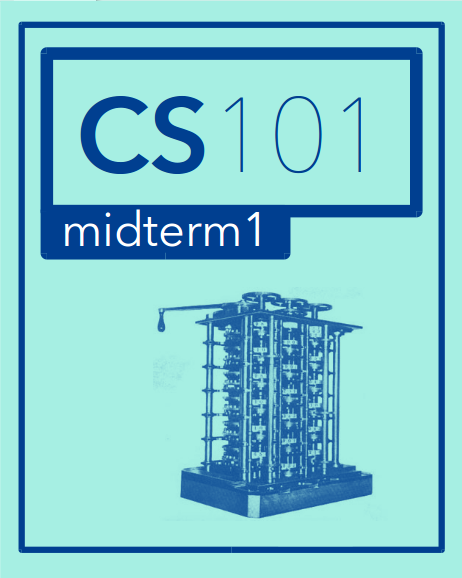
\includegraphics[width=2in]{../img/midterm1-header.png}
\end{center}

\bigskip
\noindent
\begin{itemize}
\item \textbf{Be sure to enter your \underline{NetID} and \underline{the code below} on your Scantron}.
\item Do not turn this page until instructed to do so.
\item There are 30 questions, worth 1 point each.
\item Each question has only \textbf{one} correct answer.
\item You must not communicate with other students during this test.
\item No books, notes, or electronic devices are permitted.
\item This is a 60-minute exam.
\item There are several different versions of this exam.
\end{itemize}

\bigskip\bigskip
\noindent
\textbf{\Large 1. Fill in your information:}

\bigskip
{\Large\bf
\begin{tabular}{ll}
Full Name: & \underbar{\hskip 8cm} \\[0.5em]
UIN (Student Number): & \underbar{\hskip 8cm} \\[0.5em]
NetID: & \underbar{\hskip 8cm}
\end{tabular}
}

\bigskip
\bigskip
\noindent
\textbf{\Large 2. Fill in the following answers on the Scantron form:}

%%%%%%%%%%%%%%%%%%%%%%%%%%%%%%%%%%%%%%%%%%%%%%%%%%%%%%%%%
%%%%%%%%%%%%%%%%%%%%%%%%%%%%%%%%%%%%%%%%%%%%%%%%%%%%%%%%%

\begin{enumerate}
\item[92.] E
\item[93.] A
\item[94.] A
\item[95.] C
\item[96.] B
\end{enumerate}

\newpage

% Zone 1


%%%%%%%%%%%%%%%%%%%%%%%%%%%%%%%%%%%%%%%%%%%%%%%%%%%%%%%%%



\newpage
\noindent
1. (1 point)
Consider the following program:
\begin{verbatim}
s="Hobbes"
i=0
x=-1
while i<len(s):
    if s[i]=='b':
        x=i
    i+=1
\end{verbatim}
What is the \textbf{value} of \texttt{x} after this program is executed?


\begin{enumerate}
\item[(A)]
\begin{verbatim}4\end{verbatim}

\item[(B)]
\begin{verbatim}2\end{verbatim}

\item[(C)]
\begin{verbatim}-1\end{verbatim}

\item[(D)] $\bigstar$ 
\begin{verbatim}3\end{verbatim}

\item[(E)]
\begin{verbatim}5\end{verbatim}

\end{enumerate}

\vspace*{2em}
\hrule
\vspace{2em}

\noindent {\bf Solution.} 
\vspace{2em}
\hrule height 2pt


\newpage
\noindent
2. (1 point)
Consider the following program:
\begin{verbatim}
s="G+R+A+I+L"
x=s.split("+")[1:-2]
\end{verbatim}
What is the \textbf{value} of \texttt{x} after this program is executed?


\begin{enumerate}
\item[(A)] $\bigstar$ 
\begin{verbatim}['R','A']\end{verbatim}

\item[(B)]
\begin{verbatim}None\end{verbatim}

\item[(C)]
\begin{verbatim}False\end{verbatim}

\item[(D)]
\begin{verbatim}'RAI'\end{verbatim}

\item[(E)]
\begin{verbatim}3\end{verbatim}

\end{enumerate}

\vspace*{2em}
\hrule
\vspace{2em}

\noindent {\bf Solution.} 
\vspace{2em}
\hrule height 2pt


\newpage
\noindent
3. (1 point)
Consider the following program.
\begin{verbatim}
def artificing(s):
    return s*2
    return s+"%i" % 2
    return s

s=artificing("MERLIN")
\end{verbatim}
After it is run, what is the final \textbf{value} of s?


\begin{enumerate}
\item[(A)]
\begin{verbatim}12\end{verbatim}

\item[(B)]
\begin{verbatim}"MERLIN"\end{verbatim}

\item[(C)] $\bigstar$ 
\begin{verbatim}"MERLINMERLIN"\end{verbatim}

\item[(D)]
\begin{verbatim}"MERLIN2"\end{verbatim}

\item[(E)]
\begin{verbatim}None\end{verbatim}

\end{enumerate}

\vspace*{2em}
\hrule
\vspace{2em}

\noindent {\bf Solution.} 
\vspace{2em}
\hrule height 2pt


\newpage
\noindent
4. (1 point)
Consider the following program:
\begin{verbatim}
x=str(1.2)*2
\end{verbatim}
What is the \textbf{value} of \texttt{x} after this program is executed?


\begin{enumerate}
\item[(A)]
None of the other answers are correct.

\item[(B)] $\bigstar$ 
\begin{verbatim}"1.21.2"\end{verbatim}

\item[(C)]
\begin{verbatim}2.4\end{verbatim}

\item[(D)]
\begin{verbatim}"2.4"\end{verbatim}

\item[(E)]
\begin{verbatim}"1.2*2"\end{verbatim}

\end{enumerate}

\vspace*{2em}
\hrule
\vspace{2em}

\noindent {\bf Solution.} 
\vspace{2em}
\hrule height 2pt


\newpage
\noindent
5. (1 point)
Consider the following Python program.
\begin{verbatim}
e=[1,3,5,7,9,11]
d=[0,0,0]
for i in range(0,len(e)):
    d[i%3]+=e[i]
x=d[2]
\end{verbatim}
After it is run, what is the final \textbf{value} of \texttt{x}?


\begin{enumerate}
\item[(A)]
\begin{verbatim}7\end{verbatim}

\item[(B)] $\bigstar$ 
\begin{verbatim}16\end{verbatim}

\item[(C)]
\begin{verbatim}12\end{verbatim}

\item[(D)]
\begin{verbatim}0\end{verbatim}

\item[(E)]
\begin{verbatim}8\end{verbatim}

\end{enumerate}

\vspace*{2em}
\hrule
\vspace{2em}

\noindent {\bf Solution.} 
\vspace{2em}
\hrule height 2pt


\newpage
\noindent
6. (1 point)
Consider the following program:
\begin{verbatim}
pi="3.14159"
e="2.71828"
x=pi in pi*len(e)
\end{verbatim}
What is the \textbf{type} of \texttt{x} after this program is executed?


\begin{enumerate}
\item[(A)]
\begin{verbatim}Float\end{verbatim}

\item[(B)]
\begin{verbatim}String\end{verbatim}

\item[(C)]
\begin{verbatim}None\end{verbatim}

\item[(D)] $\bigstar$ 
\begin{verbatim}Boolean\end{verbatim}

\item[(E)]
\begin{verbatim}Integer\end{verbatim}

\end{enumerate}

\vspace*{2em}
\hrule
\vspace{2em}

\noindent {\bf Solution.} 
\vspace{2em}
\hrule height 2pt


\newpage
\noindent
7. (1 point)
Consider the following program.
\begin{verbatim}
x=[]
for j in range(0,5):
    if (j%3)==0:
        x.append("-")
    if (j%4)==0:
        x.append("*")
\end{verbatim}
After it is run, what is the final \textbf{value} of \texttt{x}?


\begin{enumerate}
\item[(A)]
\begin{verbatim}["*","-","*"]\end{verbatim}

\item[(B)]
\begin{verbatim}["*","-","*"]\end{verbatim}

\item[(C)]
\begin{verbatim}["-","*"]\end{verbatim}

\item[(D)]
None of the other answers are correct.

\item[(E)] $\bigstar$ 
\begin{verbatim}["-","*","-","*"]\end{verbatim}

\end{enumerate}

\vspace*{2em}
\hrule
\vspace{2em}

\noindent {\bf Solution.} 
\vspace{2em}
\hrule height 2pt


\newpage
\noindent
8. (1 point)
Consider the following program:
\begin{verbatim}
a=["S","T","U","P","E","F","Y"]
a=a[0:4]
a.sort()
x=""
for e in a:
    x=e+x
\end{verbatim}
What is the \textbf{value} of \texttt{x} after this program is executed?


\begin{enumerate}
\item[(A)]
\begin{verbatim}"PUST"\end{verbatim}

\item[(B)]
None of the other answers are correct.

\item[(C)]
\begin{verbatim}"STUP"\end{verbatim}

\item[(D)] $\bigstar$ 
\begin{verbatim}"UTSP"\end{verbatim}

\item[(E)]
\begin{verbatim}"PSTU"\end{verbatim}

\end{enumerate}

\vspace*{2em}
\hrule
\vspace{2em}

\noindent {\bf Solution.} 
\vspace{2em}
\hrule height 2pt


\newpage
\noindent
9. (1 point)
Consider the following program:
\begin{verbatim}
x=[1,2,3]
def f(a):
    s=""
    a.reverse()
    for i in a:
        s+=str(i)
    return s

x.append(f(x))
\end{verbatim}
What is the \textbf{value} of \texttt{x} after this program is executed?


\begin{enumerate}
\item[(A)]
\begin{verbatim}[1, 2, 3, '321']\end{verbatim}

\item[(B)]
\begin{verbatim}[3, 2, 1]\end{verbatim}

\item[(C)]
\begin{verbatim}[1, 2, 3]\end{verbatim}

\item[(D)] $\bigstar$ 
\begin{verbatim}[3, 2, 1, '321']\end{verbatim}

\item[(E)]
\begin{verbatim}[1, 2, 3, 6]\end{verbatim}

\end{enumerate}

\vspace*{2em}
\hrule
\vspace{2em}

\noindent {\bf Solution.} 
\vspace{2em}
\hrule height 2pt


\newpage
\noindent
10. (1 point)
Evaluate the following expression:
\begin{verbatim}
[1,2]+[len("3")]
\end{verbatim}
What value is produced?


\begin{enumerate}
\item[(A)]
\begin{verbatim}[1,2,3]\end{verbatim}

\item[(B)]
\begin{verbatim}[1,2,"3"]\end{verbatim}

\item[(C)]
\begin{verbatim}[1,2,1,2,1,2]\end{verbatim}

\item[(D)] $\bigstar$ 
\begin{verbatim}[1,2,1]\end{verbatim}

\end{enumerate}

\vspace*{2em}
\hrule
\vspace{2em}

\noindent {\bf Solution.} 
\vspace{2em}
\hrule height 2pt


\newpage
\noindent
11. (1 point)
Consider the following program:
\begin{verbatim}
a=3
b=4
if a==3:
    a=b
elif a==4:
    a=5
else:
    b=a
\end{verbatim}
What is the \textbf{value} of a after this program is executed?


\begin{enumerate}
\item[(A)]
\begin{verbatim}3\end{verbatim}

\item[(B)] $\bigstar$ 
\begin{verbatim}4\end{verbatim}

\item[(C)]
\begin{verbatim}7\end{verbatim}

\item[(D)]
None of the other answers are correct.

\item[(E)]
\begin{verbatim}5\end{verbatim}

\end{enumerate}

\vspace*{2em}
\hrule
\vspace{2em}

\noindent {\bf Solution.} 
\vspace{2em}
\hrule height 2pt


\newpage
\noindent
12. (1 point)
Consider the following program:
\begin{verbatim}
s="TRIS %i"
t="ISEU"
x=len(s) % len(t[2:-1])
\end{verbatim}
What is the \textbf{type} of \texttt{x} after this program is executed?


\begin{enumerate}
\item[(A)]
\begin{verbatim}Boolean\end{verbatim}

\item[(B)] $\bigstar$ 
\begin{verbatim}Integer\end{verbatim}

\item[(C)]
\begin{verbatim}None\end{verbatim}

\item[(D)]
\begin{verbatim}Float\end{verbatim}

\item[(E)]
\begin{verbatim}String\end{verbatim}

\end{enumerate}

\vspace*{2em}
\hrule
\vspace{2em}

\noindent {\bf Solution.} 
\vspace{2em}
\hrule height 2pt


\newpage
\noindent
13. (1 point)
Consider the following program:
\begin{verbatim}
def fix(s):
    a=list(s)
    a.sort()
    return ''.join(a)

x=["one","two","eleven","twelve"]
s1=fix(x[0]+x[-1])
s2=fix(x[1]+x[-2])

if s1<s2:
    x.sort()
elif s1>s2:
    x.reverse()
else:
    x.append("six")
\end{verbatim}
What is the \textbf{value} of \texttt{x} after this program is executed?


\begin{enumerate}
\item[(A)]
\begin{verbatim}['twelve', 'eleven', 'two', 'one']\end{verbatim}

\item[(B)]
\begin{verbatim}['eleven', 'one', 'twelve', 'two']\end{verbatim}

\item[(C)] $\bigstar$ 
\begin{verbatim}['one', 'two', 'eleven', 'twelve', 'six']\end{verbatim}

\item[(D)]
\begin{verbatim}['two', 'twelve', 'one', 'eleven', 'six']\end{verbatim}

\item[(E)]
\begin{verbatim}['one', 'two', 'eleven', 'twelve']\end{verbatim}

\end{enumerate}

\vspace*{2em}
\hrule
\vspace{2em}

\noindent {\bf Solution.} 
\vspace{2em}
\hrule height 2pt


\newpage
\noindent
14. (1 point)
For this problem, you should compose a function which accomplishes a given task using the available code blocks arranged in the correct functional order.  \emph{We ignore indentation for this problem.}

\texttt{find\_max} should accept a \texttt{list} and return the value of the maximum item in the \texttt{list}.  (\texttt{None} is always the lowest value in any numeric comparison, so you may use it as an initializer.)

\begin{verbatim}
def find_max(my_list):
\end{verbatim}

\begin{enumerate}[1]
\item \texttt{max\_val = i}
\item \texttt{max\_val = None}
\item \texttt{for i in range(len(my\_list)):}
\item \texttt{if i > max\_val:}
\item \texttt{max\_val = my\_list[i]}
\item \texttt{return max\_val}
\item \texttt{for i in range(my\_list):}
\item \texttt{if my\_list[i] > max\_val:}
\item \texttt{print(max\_val)}
\end{enumerate}



\begin{enumerate}
\item[(A)] $\bigstar$ 
2, 3, 8, 5, 6

\item[(B)]
2, 7, 4, 5, 6

\item[(C)]
3, 2, 8, 5, 9

\item[(D)]
2, 3, 4, 1, 6

\item[(E)]
2, 3, 8, 1, 6

\end{enumerate}

\vspace*{2em}
\hrule
\vspace{2em}

\noindent {\bf Solution.} 
\vspace{2em}
\hrule height 2pt


\newpage
\noindent
15. (1 point)
Consider the following program:
\begin{verbatim}
x=0
for i in range(2,7):
    if i%3==0:
        x+=3
    elif i%2==0:
        x+=2
    else:
        x+=1
\end{verbatim}
What is the \textbf{value} of \texttt{x} after this program is executed?


\begin{enumerate}
\item[(A)] $\bigstar$ 
\begin{verbatim}11\end{verbatim}

\item[(B)]
\begin{verbatim}10\end{verbatim}

\item[(C)]
\begin{verbatim}12\end{verbatim}

\item[(D)]
\begin{verbatim}13\end{verbatim}

\item[(E)]
\begin{verbatim}14\end{verbatim}

\end{enumerate}

\vspace*{2em}
\hrule
\vspace{2em}

\noindent {\bf Solution.} 
\vspace{2em}
\hrule height 2pt


\newpage
\noindent
16. (1 point)
Consider the following program.
\begin{verbatim}
s="ABCBA"
x=0
y=len(s)-1
while s[x]==s[y] and x<=y:
    x+=1
    y-=1
\end{verbatim}
After it is run, what is the final \textbf{value} of \texttt{x}?


\begin{enumerate}
\item[(A)]
\begin{verbatim}1\end{verbatim}

\item[(B)]
\begin{verbatim}0\end{verbatim}

\item[(C)] $\bigstar$ 
\begin{verbatim}3\end{verbatim}

\item[(D)]
\begin{verbatim}2\end{verbatim}

\item[(E)]
\begin{verbatim}4\end{verbatim}

\end{enumerate}

\vspace*{2em}
\hrule
\vspace{2em}

\noindent {\bf Solution.} 
\vspace{2em}
\hrule height 2pt


\newpage
\noindent
17. (1 point)
Consider the following program:
\begin{verbatim}
x=3
a=7
if (a%3)==2:
    x=x**2
elif(a%3)==1:
    x=x**1
else:
    x=x**0
\end{verbatim}
What is the \textbf{value} of \texttt{x} after this program is executed?


\begin{enumerate}
\item[(A)]
None of the other answers are correct.

\item[(B)]
\begin{verbatim}9\end{verbatim}

\item[(C)]
\begin{verbatim}7\end{verbatim}

\item[(D)] $\bigstar$ 
\begin{verbatim}3\end{verbatim}

\item[(E)]
\begin{verbatim}1\end{verbatim}

\end{enumerate}

\vspace*{2em}
\hrule
\vspace{2em}

\noindent {\bf Solution.} 
\vspace{2em}
\hrule height 2pt


\newpage
\noindent
18. (1 point)
Consider the following program:
\begin{verbatim}
a=["merlin","sir agravaine","king pellinore"]
b=[ ]
for i in range(1,3):
    b.append(a[0-i].title())
\end{verbatim}
What is the \textbf{value} of b after this program is executed?


\begin{enumerate}
\item[(A)]
\begin{verbatim}['Merlin', 'King Pellinore', 'Sir Agravaine']\end{verbatim}

\item[(B)]
\begin{verbatim}[ ]\end{verbatim}

\item[(C)] $\bigstar$ 
\begin{verbatim}['King Pellinore', 'Sir Agravaine']\end{verbatim}

\item[(D)]
\begin{verbatim}['Sir Agravaine', 'King Pellinore']\end{verbatim}

\item[(E)]
\begin{verbatim}['King Pellinore', 'Sir Agravaine', 'Merlin']\end{verbatim}

\end{enumerate}

\vspace*{2em}
\hrule
\vspace{2em}

\noindent {\bf Solution.} 
\vspace{2em}
\hrule height 2pt


\newpage
\noindent
19. (1 point)
Consider the following program:
\begin{verbatim}
x=[1,2,3,4,5,6,7,8,9]
x=x[2:-2]
i=1
while i <= 3:
    x[i]+=1
    i+=1
\end{verbatim}
What is the \textbf{value} of \texttt{x} after this program is executed?


\begin{enumerate}
\item[(A)]
\begin{verbatim}[2, 4, 5, 6, 7, 7]\end{verbatim}

\item[(B)] $\bigstar$ 
\begin{verbatim}[3, 5, 6, 7, 7]\end{verbatim}

\item[(C)]
\begin{verbatim}[3, 5, 7, 7]\end{verbatim}

\item[(D)]
\begin{verbatim}[2, 4, 5, 5, 7, 7]\end{verbatim}

\item[(E)]
\begin{verbatim}[3, 5, 6, 7, 7, 8]\end{verbatim}

\end{enumerate}

\vspace*{2em}
\hrule
\vspace{2em}

\noindent {\bf Solution.} 
\vspace{2em}
\hrule height 2pt


\newpage
\noindent
20. (1 point)
Consider the following program:
\begin{verbatim}
x="KING ARTHUR-MORGANA LEFAY-SIR BEDIVERE".split("-")
y=x
y.reverse()
\end{verbatim}
What is the \textbf{value} of \texttt{x} after this program is executed?


\begin{enumerate}
\item[(A)]
\begin{verbatim}['KING ARTHUR', 'MORGANA LEFAY', 'SIR BEDIVERE']\end{verbatim}

\item[(B)]
\begin{verbatim}None\end{verbatim}

\item[(C)]
\begin{verbatim}['BEDIVERE', 'LEFAY-SIR', 'ARTHUR-MORGANA', 'KING']\end{verbatim}

\item[(D)]
\begin{verbatim}['KING', 'ARTHUR-MORGANA', 'LEFAY-SIR', 'BEDIVERE']\end{verbatim}

\item[(E)] $\bigstar$ 
\begin{verbatim}['SIR BEDIVERE', 'MORGANA LEFAY', 'KING ARTHUR']\end{verbatim}

\end{enumerate}

\vspace*{2em}
\hrule
\vspace{2em}

\noindent {\bf Solution.} 
\vspace{2em}
\hrule height 2pt


\newpage
\noindent
21. (1 point)
Consider the following program.
\begin{verbatim}
x=0
i=1
while(i*i)<=9:
    x=x+(i*i)
    i=i+1
\end{verbatim}
After it is run, what is the final \textbf{value} of \texttt{x}?


\begin{enumerate}
\item[(A)] $\bigstar$ 
\begin{verbatim}14\end{verbatim}

\item[(B)]
\begin{verbatim}4\end{verbatim}

\item[(C)]
\begin{verbatim}3\end{verbatim}

\item[(D)]
\begin{verbatim}30\end{verbatim}

\item[(E)]
\begin{verbatim}5\end{verbatim}

\end{enumerate}

\vspace*{2em}
\hrule
\vspace{2em}

\noindent {\bf Solution.} 
\vspace{2em}
\hrule height 2pt


\newpage
\noindent
22. (1 point)
What is the result of the following expression?
\begin{verbatim}
[ 1, 2, 3 ] * 3
\end{verbatim}


\begin{enumerate}
\item[(A)]
\begin{verbatim}(3, 6, 9)\end{verbatim}

\item[(B)]
\begin{verbatim}[1.0, 2.0, 3.0, 1.0, 2.0, 3.0, 1.0, 2.0, 3.0]\end{verbatim}

\item[(C)]
\begin{verbatim}[3.0, 6.0, 9.0]\end{verbatim}

\item[(D)] $\bigstar$ 
\begin{verbatim}[1, 2, 3, 1, 2, 3, 1, 2, 3]\end{verbatim}

\item[(E)]
\begin{verbatim}[3, 6, 9]\end{verbatim}

\end{enumerate}

\vspace*{2em}
\hrule
\vspace{2em}

\noindent {\bf Solution.} 
\vspace{2em}
\hrule height 2pt


\newpage
\noindent
23. (1 point)
Consider the following program:
\begin{verbatim}
i=2
x=3
while i < 7:
    x+=i
    i+=2
\end{verbatim}
What is the \textbf{value} of \texttt{x} after this program is executed?


\begin{enumerate}
\item[(A)]
\begin{verbatim}11\end{verbatim}

\item[(B)]
\begin{verbatim}13\end{verbatim}

\item[(C)]
\begin{verbatim}14\end{verbatim}

\item[(D)]
\begin{verbatim}12\end{verbatim}

\item[(E)] $\bigstar$ 
\begin{verbatim}15\end{verbatim}

\end{enumerate}

\vspace*{2em}
\hrule
\vspace{2em}

\noindent {\bf Solution.} 
\vspace{2em}
\hrule height 2pt


\newpage
\noindent
24. (1 point)
Evaluate the following expression:
\begin{verbatim}
len("ABCDE"[1:4])
\end{verbatim}
What value is produced?


\begin{enumerate}
\item[(A)]
1

\item[(B)]
5

\item[(C)] $\bigstar$ 
3

\item[(D)]
4

\end{enumerate}

\vspace*{2em}
\hrule
\vspace{2em}

\noindent {\bf Solution.} 
\vspace{2em}
\hrule height 2pt


\newpage
\noindent
25. (1 point)
Consider the following incomplete function.
\begin{verbatim}
def ismultiple(m,n):
    if ???:
        return False
    else:
        return True
\end{verbatim}
The function is intended to return True if the input parameter m is a multiple of parameter n and False otherwise. For example, \verb|ismultiple(4,2)| should return \verb|True|, but \verb|ismultiple(5,3)| should return \verb|False|. What should replace the three question marks to complete the function?


\begin{enumerate}
\item[(A)] $\bigstar$ 
\begin{verbatim}(m % n) != 0 \end{verbatim}

\item[(B)]
\begin{verbatim}(n // m) == 0 \end{verbatim}

\item[(C)]
\begin{verbatim}(n % m) == 0 \end{verbatim}

\item[(D)]
\begin{verbatim}(m // n) != 0 \end{verbatim}

\end{enumerate}

\vspace*{2em}
\hrule
\vspace{2em}

\noindent {\bf Solution.} 
\vspace{2em}
\hrule height 2pt


\newpage
\noindent
26. (1 point)
Consider the following incomplete Python program.
\begin{verbatim}
s="".join(["2","2","0","1"])
x=0
for i in range(len(s)-1):
    x+=int(???)
\end{verbatim}
What should replace the three question marks so the resulting value of \texttt{x} is 43?


\begin{enumerate}
\item[(A)]
\begin{verbatim}s[i:i-1]\end{verbatim}

\item[(B)] $\bigstar$ 
\begin{verbatim}s[i:i+2]\end{verbatim}

\item[(C)]
\begin{verbatim}s[i+1:i+2]\end{verbatim}

\item[(D)]
\begin{verbatim}s[i:i+1]\end{verbatim}

\end{enumerate}

\vspace*{2em}
\hrule
\vspace{2em}

\noindent {\bf Solution.} 
\vspace{2em}
\hrule height 2pt


\newpage
\noindent
27. (1 point)
Consider the following incomplete program.
\begin{verbatim}
sum=0
???:
    sum=sum+i

\end{verbatim}
The program is intended to sum all of the integers between 1 and 100 (inclusive). What should replace the three question marks to complete the program?


\begin{enumerate}
\item[(A)]
\begin{verbatim}while i<=100 \end{verbatim}

\item[(B)]
\begin{verbatim}while i in range(100)\end{verbatim}

\item[(C)]
\begin{verbatim}for i in range(0,100)\end{verbatim}

\item[(D)] $\bigstar$ 
\begin{verbatim}for i in range(1,101) \end{verbatim}

\end{enumerate}

\vspace*{2em}
\hrule
\vspace{2em}

\noindent {\bf Solution.} 
\vspace{2em}
\hrule height 2pt


\newpage
\noindent
28. (1 point)
How can the following mathematical equation be implemented as a Python expression? Assume \verb|a|, \verb|b|, and \verb|cos| have already been defined.
$$a^b \cos(a - b)$$


\begin{enumerate}
\item[(A)] $\bigstar$ 
\begin{verbatim}(a**b)*cos(a-b)\end{verbatim}

\item[(B)]
\begin{verbatim}(a^b)*cos(a-b)\end{verbatim}

\item[(C)]
\begin{verbatim}(a**b)cos(a-b)\end{verbatim}

\item[(D)]
\begin{verbatim}(b^a)cos(a-b)\end{verbatim}

\item[(E)]
None of the other answers are correct.

\end{enumerate}

\vspace*{2em}
\hrule
\vspace{2em}

\noindent {\bf Solution.} 
\vspace{2em}
\hrule height 2pt


\newpage
\noindent
29. (1 point)
Consider the following program:
\begin{verbatim}
s="ECTOR"
t="GAWAIN"
x=len(str(s.isupper()))-t.find("A")
\end{verbatim}
What is the \textbf{type} of \texttt{x} after this program is executed?


\begin{enumerate}
\item[(A)] $\bigstar$ 
\begin{verbatim}Integer\end{verbatim}

\item[(B)]
\begin{verbatim}String\end{verbatim}

\item[(C)]
\begin{verbatim}Float\end{verbatim}

\item[(D)]
\begin{verbatim}Boolean\end{verbatim}

\item[(E)]
\begin{verbatim}None\end{verbatim}

\end{enumerate}

\vspace*{2em}
\hrule
\vspace{2em}

\noindent {\bf Solution.} 
\vspace{2em}
\hrule height 2pt


\newpage
\noindent
30. (1 point)
Consider the following program.
\begin{verbatim}
kay = 2
wart = 3

def knight(kay,wart):
    wart += 2
    kay += 3
    return wart + kay

wart = knight(kay, kay) + knight(wart, wart)
\end{verbatim}
After it is run, what is the final \textbf{value} of \texttt{wart}?


\begin{enumerate}
\item[(A)]
\begin{verbatim}5\end{verbatim}

\item[(B)]
\begin{verbatim}2\end{verbatim}

\item[(C)] $\bigstar$ 
None of the other answers are correct.

\item[(D)]
\begin{verbatim}3\end{verbatim}

\end{enumerate}

\vspace*{2em}
\hrule
\vspace{2em}

\noindent {\bf Solution.} 
\vspace{2em}
\hrule height 2pt

%%%%%%%%%%%%%%%%%%%%%%%%%%%%%%%%%%%%%%%%%%%%%%%%%%%%%%%%%%%%%%%%%%%%%%
%%%%%%%%%%%%%%%%%%%%%%%%%%%%%%%%%%%%%%%%%%%%%%%%%%%%%%%%%%%%%%%%%%%%%%
%%%%%%%%%%%%%%%%%%%%%%%%%%%%%%%%%%%%%%%%%%%%%%%%%%%%%%%%%%%%%%%%%%%%%%
%%%%%%%%%%%%%%%%%%%%%%%%%%%%%%%%%%%%%%%%%%%%%%%%%%%%%%%%%%%%%%%%%%%%%%
% Exam number 6

\message{Exam 6/50}
\cleardoublepage
\setcounter{page}{1}


\begin{center}
%\textbf{\Large CS 101 Midterm \#1}
%
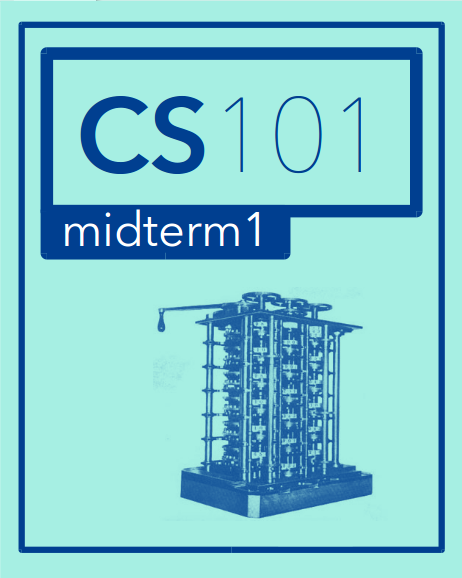
\includegraphics[width=2in]{../img/midterm1-header.png}
\end{center}

\bigskip
\noindent
\begin{itemize}
\item \textbf{Be sure to enter your \underline{NetID} and \underline{the code below} on your Scantron}.
\item Do not turn this page until instructed to do so.
\item There are 30 questions, worth 1 point each.
\item Each question has only \textbf{one} correct answer.
\item You must not communicate with other students during this test.
\item No books, notes, or electronic devices are permitted.
\item This is a 60-minute exam.
\item There are several different versions of this exam.
\end{itemize}

\bigskip\bigskip
\noindent
\textbf{\Large 1. Fill in your information:}

\bigskip
{\Large\bf
\begin{tabular}{ll}
Full Name: & \underbar{\hskip 8cm} \\[0.5em]
UIN (Student Number): & \underbar{\hskip 8cm} \\[0.5em]
NetID: & \underbar{\hskip 8cm}
\end{tabular}
}

\bigskip
\bigskip
\noindent
\textbf{\Large 2. Fill in the following answers on the Scantron form:}

%%%%%%%%%%%%%%%%%%%%%%%%%%%%%%%%%%%%%%%%%%%%%%%%%%%%%%%%%
%%%%%%%%%%%%%%%%%%%%%%%%%%%%%%%%%%%%%%%%%%%%%%%%%%%%%%%%%

\begin{enumerate}
\item[92.] A
\item[93.] B
\item[94.] A
\item[95.] E
\item[96.] E
\end{enumerate}

\newpage

% Zone 1


%%%%%%%%%%%%%%%%%%%%%%%%%%%%%%%%%%%%%%%%%%%%%%%%%%%%%%%%%



\newpage
\noindent
1. (1 point)
Consider the following program.
\begin{verbatim}
s="ABCBA"
x=0
y=len(s)-1
while s[x]==s[y] and x<y:
    x+=1
    y-=1
\end{verbatim}
After it is run, what is the final \textbf{value} of \texttt{x}?


\begin{enumerate}
\item[(A)]
\begin{verbatim}3\end{verbatim}

\item[(B)]
\begin{verbatim}4\end{verbatim}

\item[(C)]
\begin{verbatim}0\end{verbatim}

\item[(D)] $\bigstar$ 
\begin{verbatim}2\end{verbatim}

\item[(E)]
\begin{verbatim}1\end{verbatim}

\end{enumerate}

\vspace*{2em}
\hrule
\vspace{2em}

\noindent {\bf Solution.} 
\vspace{2em}
\hrule height 2pt


\newpage
\noindent
2. (1 point)
Consider the following program:
\begin{verbatim}
s="TRIS %i"
t="ISEU"
x=s % len(t)
\end{verbatim}
What is the \textbf{type} of \texttt{x} after this program is executed?


\begin{enumerate}
\item[(A)] $\bigstar$ 
\begin{verbatim}String\end{verbatim}

\item[(B)]
\begin{verbatim}Boolean\end{verbatim}

\item[(C)]
\begin{verbatim}None\end{verbatim}

\item[(D)]
\begin{verbatim}Integer\end{verbatim}

\item[(E)]
\begin{verbatim}Float\end{verbatim}

\end{enumerate}

\vspace*{2em}
\hrule
\vspace{2em}

\noindent {\bf Solution.} 
\vspace{2em}
\hrule height 2pt


\newpage
\noindent
3. (1 point)
Consider the following program:
\begin{verbatim}
s="Calvin"
i=0
x=-1
while i<len(s):
    if s[i]=='b':
        x=i
    i+=1
\end{verbatim}
What is the \textbf{value} of \texttt{x} after this program is executed?


\begin{enumerate}
\item[(A)]
\begin{verbatim}3\end{verbatim}

\item[(B)]
\begin{verbatim}0\end{verbatim}

\item[(C)] $\bigstar$ 
\begin{verbatim}-1\end{verbatim}

\item[(D)]
\begin{verbatim}5\end{verbatim}

\item[(E)]
\begin{verbatim}6\end{verbatim}

\end{enumerate}

\vspace*{2em}
\hrule
\vspace{2em}

\noindent {\bf Solution.} 
\vspace{2em}
\hrule height 2pt


\newpage
\noindent
4. (1 point)
Consider the following program:
\begin{verbatim}
a=3
b=4
if a==3:
    a=b
elif a==4:
    a=5
else:
    b=a
\end{verbatim}
What is the \textbf{value} of a after this program is executed?


\begin{enumerate}
\item[(A)]
\begin{verbatim}5\end{verbatim}

\item[(B)]
\begin{verbatim}7\end{verbatim}

\item[(C)] $\bigstar$ 
\begin{verbatim}4\end{verbatim}

\item[(D)]
None of the other answers are correct.

\item[(E)]
\begin{verbatim}3\end{verbatim}

\end{enumerate}

\vspace*{2em}
\hrule
\vspace{2em}

\noindent {\bf Solution.} 
\vspace{2em}
\hrule height 2pt


\newpage
\noindent
5. (1 point)
Consider the following program.
\begin{verbatim}
kay = 2
wart = 3

def knight(kay,wart):
    wart += 2
    kay += 3
    return wart + kay

kay = knight(wart, kay) + knight(kay, wart)
\end{verbatim}
After it is run, what is the final \textbf{value} of \texttt{kay}?


\begin{enumerate}
\item[(A)]
\begin{verbatim}2\end{verbatim}

\item[(B)] $\bigstar$ 
None of the other answers are correct.

\item[(C)]
\begin{verbatim}5\end{verbatim}

\item[(D)]
\begin{verbatim}3\end{verbatim}

\end{enumerate}

\vspace*{2em}
\hrule
\vspace{2em}

\noindent {\bf Solution.} 
\vspace{2em}
\hrule height 2pt


\newpage
\noindent
6. (1 point)
Consider the following program:
\begin{verbatim}
s="ECTOR"
t="GAWAIN"
x=(len(s)/(len(t)-1))+1
\end{verbatim}
What is the \textbf{type} of \texttt{x} after this program is executed?


\begin{enumerate}
\item[(A)]
\begin{verbatim}Boolean\end{verbatim}

\item[(B)]
\begin{verbatim}String\end{verbatim}

\item[(C)]
\begin{verbatim}None\end{verbatim}

\item[(D)] $\bigstar$ 
\begin{verbatim}Float\end{verbatim}

\item[(E)]
\begin{verbatim}Integer\end{verbatim}

\end{enumerate}

\vspace*{2em}
\hrule
\vspace{2em}

\noindent {\bf Solution.} 
\vspace{2em}
\hrule height 2pt


\newpage
\noindent
7. (1 point)
Evaluate the following expression:
\begin{verbatim}
len("ABCD"[0:3])
\end{verbatim}
What value is produced?


\begin{enumerate}
\item[(A)]
2

\item[(B)]
1

\item[(C)]
4

\item[(D)] $\bigstar$ 
3

\end{enumerate}

\vspace*{2em}
\hrule
\vspace{2em}

\noindent {\bf Solution.} 
\vspace{2em}
\hrule height 2pt


\newpage
\noindent
8. (1 point)
Consider the following program:
\begin{verbatim}
a=["merlin","sir agravaine","king pellinore"]
b=[ ]
for i in range(0,3):
    b.append(a[0-i].title())
\end{verbatim}
What is the \textbf{value} of b after this program is executed?


\begin{enumerate}
\item[(A)]
\begin{verbatim}['King Pellinore', 'Sir Agravaine', 'Merlin']\end{verbatim}

\item[(B)]
\begin{verbatim}['King Pellinore', 'Sir Agravaine']\end{verbatim}

\item[(C)]
\begin{verbatim}['Sir Agravaine', 'King Pellinore']\end{verbatim}

\item[(D)] $\bigstar$ 
\begin{verbatim}['Merlin', 'King Pellinore', 'Sir Agravaine']\end{verbatim}

\item[(E)]
\begin{verbatim}[ ]\end{verbatim}

\end{enumerate}

\vspace*{2em}
\hrule
\vspace{2em}

\noindent {\bf Solution.} 
\vspace{2em}
\hrule height 2pt


\newpage
\noindent
9. (1 point)
How can the following mathematical equation be implemented as a Python expression? Assume \verb|a|, \verb|b|, and \verb|cos| have already been defined.
$$a^b \cos(a - b)$$


\begin{enumerate}
\item[(A)]
\begin{verbatim}(a^b)*cos(a-b)\end{verbatim}

\item[(B)]
\begin{verbatim}(b^a)cos(a-b)\end{verbatim}

\item[(C)]
None of the other answers are correct.

\item[(D)]
\begin{verbatim}(a**b)cos(a-b)\end{verbatim}

\item[(E)] $\bigstar$ 
\begin{verbatim}(a**b)*cos(a-b)\end{verbatim}

\end{enumerate}

\vspace*{2em}
\hrule
\vspace{2em}

\noindent {\bf Solution.} 
\vspace{2em}
\hrule height 2pt


\newpage
\noindent
10. (1 point)
Consider the following program:
\begin{verbatim}
x=0
for i in range(2,7):
    if i%3==0:
        x+=3
    elif i%2==0:
        x+=2
    else:
        x+=1
\end{verbatim}
What is the \textbf{value} of \texttt{x} after this program is executed?


\begin{enumerate}
\item[(A)]
\begin{verbatim}13\end{verbatim}

\item[(B)]
\begin{verbatim}12\end{verbatim}

\item[(C)] $\bigstar$ 
\begin{verbatim}11\end{verbatim}

\item[(D)]
\begin{verbatim}14\end{verbatim}

\item[(E)]
\begin{verbatim}10\end{verbatim}

\end{enumerate}

\vspace*{2em}
\hrule
\vspace{2em}

\noindent {\bf Solution.} 
\vspace{2em}
\hrule height 2pt


\newpage
\noindent
11. (1 point)
Consider the following incomplete function.
\begin{verbatim}
def isdivisible(m,n):
    if ???:
        return False
    else:
        return True
\end{verbatim}
The function is intended to return True if the input parameter m is evenly divisible by the parameter n and False otherwise. For example, \verb|isdivisible(4,2)| should return \verb|True|, but \verb|isdivisible(5,3)| should return \verb|False|. What should replace the three question marks to complete the function?


\begin{enumerate}
\item[(A)] $\bigstar$ 
\begin{verbatim}(m % n) != 0 \end{verbatim}

\item[(B)]
\begin{verbatim}(n // m) == 0 \end{verbatim}

\item[(C)]
\begin{verbatim}(m // n) != 0 \end{verbatim}

\item[(D)]
\begin{verbatim}(n % m) == 0 \end{verbatim}

\end{enumerate}

\vspace*{2em}
\hrule
\vspace{2em}

\noindent {\bf Solution.} 
\vspace{2em}
\hrule height 2pt


\newpage
\noindent
12. (1 point)
Consider the following program:
\begin{verbatim}
i=2
x=3
while i < 7:
    x+=i
    i+=2
\end{verbatim}
What is the \textbf{value} of \texttt{x} after this program is executed?


\begin{enumerate}
\item[(A)]
\begin{verbatim}14\end{verbatim}

\item[(B)]
\begin{verbatim}13\end{verbatim}

\item[(C)] $\bigstar$ 
\begin{verbatim}15\end{verbatim}

\item[(D)]
\begin{verbatim}11\end{verbatim}

\item[(E)]
\begin{verbatim}12\end{verbatim}

\end{enumerate}

\vspace*{2em}
\hrule
\vspace{2em}

\noindent {\bf Solution.} 
\vspace{2em}
\hrule height 2pt


\newpage
\noindent
13. (1 point)
Consider the following incomplete Python program.
\begin{verbatim}
s="".join(["1","0","2","1"])
x=0
for i in range(len(s)-1):
    x+=int(???)
\end{verbatim}
What should replace the three question marks so the resulting value of \texttt{x} is 33?


\begin{enumerate}
\item[(A)]
\begin{verbatim}s[i:i-1]\end{verbatim}

\item[(B)] $\bigstar$ 
\begin{verbatim}s[i:i+2]\end{verbatim}

\item[(C)]
\begin{verbatim}s[i:i+1]\end{verbatim}

\item[(D)]
\begin{verbatim}s[i+1:i+2]\end{verbatim}

\end{enumerate}

\vspace*{2em}
\hrule
\vspace{2em}

\noindent {\bf Solution.} 
\vspace{2em}
\hrule height 2pt


\newpage
\noindent
14. (1 point)
Evaluate the following expression:
\begin{verbatim}
[1,2]*len("3")
\end{verbatim}
What value is produced?


\begin{enumerate}
\item[(A)] $\bigstar$ 
\begin{verbatim}[1,2]\end{verbatim}

\item[(B)]
\begin{verbatim}[1,2,1,2,1,2]\end{verbatim}

\item[(C)]
\begin{verbatim}[1,2,1]\end{verbatim}

\item[(D)]
\begin{verbatim}[1,2,3]\end{verbatim}

\end{enumerate}

\vspace*{2em}
\hrule
\vspace{2em}

\noindent {\bf Solution.} 
\vspace{2em}
\hrule height 2pt


\newpage
\noindent
15. (1 point)
Consider the following program.
\begin{verbatim}
x=[]
for j in range(0,5):
    if (j%3)==0:
        x.append("-")
    if (j%4)==0:
        x.append("*")
\end{verbatim}
After it is run, what is the final \textbf{value} of \texttt{x}?


\begin{enumerate}
\item[(A)]
\begin{verbatim}["*","-","*"]\end{verbatim}

\item[(B)]
\begin{verbatim}["-","*"]\end{verbatim}

\item[(C)]
None of the other answers are correct.

\item[(D)] $\bigstar$ 
\begin{verbatim}["-","*","-","*"]\end{verbatim}

\item[(E)]
\begin{verbatim}["*","-","*"]\end{verbatim}

\end{enumerate}

\vspace*{2em}
\hrule
\vspace{2em}

\noindent {\bf Solution.} 
\vspace{2em}
\hrule height 2pt


\newpage
\noindent
16. (1 point)
Consider the following program:
\begin{verbatim}
x="KING ARTHUR-MORGANA LEFAY-SIR BEDIVERE".split("-")
y=x[:]
y.reverse()
\end{verbatim}
What is the \textbf{value} of \texttt{x} after this program is executed?


\begin{enumerate}
\item[(A)] $\bigstar$ 
\begin{verbatim}['KING ARTHUR', 'MORGANA LEFAY', 'SIR BEDIVERE']\end{verbatim}

\item[(B)]
\begin{verbatim}['SIR BEDIVERE', 'MORGANA LEFAY', 'KING ARTHUR']\end{verbatim}

\item[(C)]
\begin{verbatim}['BEDIVERE', 'LEFAY-SIR', 'ARTHUR-MORGANA', 'KING']\end{verbatim}

\item[(D)]
\begin{verbatim}None\end{verbatim}

\item[(E)]
\begin{verbatim}['KING', 'ARTHUR-MORGANA', 'LEFAY-SIR', 'BEDIVERE']\end{verbatim}

\end{enumerate}

\vspace*{2em}
\hrule
\vspace{2em}

\noindent {\bf Solution.} 
\vspace{2em}
\hrule height 2pt


\newpage
\noindent
17. (1 point)
Consider the following program:
\begin{verbatim}
x=[1,2,3]
def f(a):
    s=""
    a.reverse()
    for i in a:
        s+=str(i)
    return s

x.append(f(x))
\end{verbatim}
What is the \textbf{value} of \texttt{x} after this program is executed?


\begin{enumerate}
\item[(A)]
\begin{verbatim}[1, 2, 3, 6]\end{verbatim}

\item[(B)]
\begin{verbatim}[3, 2, 1]\end{verbatim}

\item[(C)] $\bigstar$ 
\begin{verbatim}[3, 2, 1, '321']\end{verbatim}

\item[(D)]
\begin{verbatim}[1, 2, 3, '321']\end{verbatim}

\item[(E)]
\begin{verbatim}[1, 2, 3]\end{verbatim}

\end{enumerate}

\vspace*{2em}
\hrule
\vspace{2em}

\noindent {\bf Solution.} 
\vspace{2em}
\hrule height 2pt


\newpage
\noindent
18. (1 point)
Consider the following Python program.
\begin{verbatim}
e=[1,3,5,7,9,11]
d=[0,0,0]
for i in range(0,len(e)):
    d[i%3]+=e[i]
x=d[2]
\end{verbatim}
After it is run, what is the final \textbf{value} of \texttt{x}?


\begin{enumerate}
\item[(A)]
\begin{verbatim}12\end{verbatim}

\item[(B)]
\begin{verbatim}8\end{verbatim}

\item[(C)]
\begin{verbatim}0\end{verbatim}

\item[(D)] $\bigstar$ 
\begin{verbatim}16\end{verbatim}

\item[(E)]
\begin{verbatim}7\end{verbatim}

\end{enumerate}

\vspace*{2em}
\hrule
\vspace{2em}

\noindent {\bf Solution.} 
\vspace{2em}
\hrule height 2pt


\newpage
\noindent
19. (1 point)
Consider the following incomplete program.
\begin{verbatim}
sum=0
???:
    sum=sum+i

\end{verbatim}
The program is intended to sum all of the integers between 1 and 100 (inclusive). What should replace the three question marks to complete the program?


\begin{enumerate}
\item[(A)]
\begin{verbatim}while i<=100 \end{verbatim}

\item[(B)]
\begin{verbatim}while i in range(100)\end{verbatim}

\item[(C)] $\bigstar$ 
\begin{verbatim}for i in range(1,101) \end{verbatim}

\item[(D)]
\begin{verbatim}for i in range(0,100)\end{verbatim}

\end{enumerate}

\vspace*{2em}
\hrule
\vspace{2em}

\noindent {\bf Solution.} 
\vspace{2em}
\hrule height 2pt


\newpage
\noindent
20. (1 point)
Consider the following program.
\begin{verbatim}
def artificing(s):
    return s*2
    return s+"%i" % 2
    return s

s=artificing("MERLIN")
\end{verbatim}
After it is run, what is the final \textbf{value} of s?


\begin{enumerate}
\item[(A)]
\begin{verbatim}"MERLIN"\end{verbatim}

\item[(B)]
\begin{verbatim}"MERLIN2"\end{verbatim}

\item[(C)]
\begin{verbatim}12\end{verbatim}

\item[(D)]
\begin{verbatim}None\end{verbatim}

\item[(E)] $\bigstar$ 
\begin{verbatim}"MERLINMERLIN"\end{verbatim}

\end{enumerate}

\vspace*{2em}
\hrule
\vspace{2em}

\noindent {\bf Solution.} 
\vspace{2em}
\hrule height 2pt


\newpage
\noindent
21. (1 point)
Consider the following program:
\begin{verbatim}
s="-B-O-R-S-"
x=s.split("-")[2:-2]
\end{verbatim}
What is the \textbf{value} of \texttt{x} after this program is executed?


\begin{enumerate}
\item[(A)]
\begin{verbatim}None\end{verbatim}

\item[(B)]
\begin{verbatim}'ORS'\end{verbatim}

\item[(C)] $\bigstar$ 
\begin{verbatim}['O', 'R']\end{verbatim}

\item[(D)]
\begin{verbatim}False\end{verbatim}

\item[(E)]
\begin{verbatim}''\end{verbatim}

\end{enumerate}

\vspace*{2em}
\hrule
\vspace{2em}

\noindent {\bf Solution.} 
\vspace{2em}
\hrule height 2pt


\newpage
\noindent
22. (1 point)
Consider the following program:
\begin{verbatim}
pi="3.14159"
e="2.71828"
x=pi*len(e)+pi
\end{verbatim}
What is the \textbf{type} of \texttt{x} after this program is executed?


\begin{enumerate}
\item[(A)]
\begin{verbatim}Integer\end{verbatim}

\item[(B)]
\begin{verbatim}None\end{verbatim}

\item[(C)]
\begin{verbatim}Boolean\end{verbatim}

\item[(D)]
\begin{verbatim}Float\end{verbatim}

\item[(E)] $\bigstar$ 
\begin{verbatim}String\end{verbatim}

\end{enumerate}

\vspace*{2em}
\hrule
\vspace{2em}

\noindent {\bf Solution.} 
\vspace{2em}
\hrule height 2pt


\newpage
\noindent
23. (1 point)
What is the result of the following expression?
\begin{verbatim}
[ 1, 2, 3 ] * 3
\end{verbatim}


\begin{enumerate}
\item[(A)]
\begin{verbatim}[1.0, 2.0, 3.0, 1.0, 2.0, 3.0, 1.0, 2.0, 3.0]\end{verbatim}

\item[(B)] $\bigstar$ 
\begin{verbatim}[1, 2, 3, 1, 2, 3, 1, 2, 3]\end{verbatim}

\item[(C)]
\begin{verbatim}(3, 6, 9)\end{verbatim}

\item[(D)]
\begin{verbatim}[3, 6, 9]\end{verbatim}

\item[(E)]
\begin{verbatim}[3.0, 6.0, 9.0]\end{verbatim}

\end{enumerate}

\vspace*{2em}
\hrule
\vspace{2em}

\noindent {\bf Solution.} 
\vspace{2em}
\hrule height 2pt


\newpage
\noindent
24. (1 point)
Consider the following program:
\begin{verbatim}
a=["A","C","C","I","O"]
a.sort()
a[0]=a[-1]
x=""
for e in a:
    x=x+e
\end{verbatim}
What is the \textbf{value} of \texttt{x} after this program is executed?


\begin{enumerate}
\item[(A)]
\begin{verbatim}"ICCOI"\end{verbatim}

\item[(B)]
None of the other answers are correct.

\item[(C)]
\begin{verbatim}"ACCIA"\end{verbatim}

\item[(D)]
\begin{verbatim}"ACCOA"\end{verbatim}

\item[(E)] $\bigstar$ 
\begin{verbatim}"OCCIO"\end{verbatim}

\end{enumerate}

\vspace*{2em}
\hrule
\vspace{2em}

\noindent {\bf Solution.} 
\vspace{2em}
\hrule height 2pt


\newpage
\noindent
25. (1 point)
For this problem, you should compose a function which accomplishes a given task using the available code blocks arranged in the correct functional order.  \emph{We ignore indentation for this problem.}

\texttt{find\_max} should accept a \texttt{list} and return the value of the maximum item in the \texttt{list}.  (\texttt{None} is always the lowest value in any numeric comparison, so you may use it as an initializer.)

\begin{verbatim}
def find_max(my_list):
\end{verbatim}

\begin{enumerate}[1]
\item \texttt{max\_val = i}
\item \texttt{max\_val = None}
\item \texttt{for i in range(len(my\_list)):}
\item \texttt{if i > max\_val:}
\item \texttt{max\_val = my\_list[i]}
\item \texttt{return max\_val}
\item \texttt{for i in range(my\_list):}
\item \texttt{if my\_list[i] > max\_val:}
\item \texttt{print(max\_val)}
\end{enumerate}



\begin{enumerate}
\item[(A)] $\bigstar$ 
2, 3, 8, 5, 6

\item[(B)]
2, 3, 8, 1, 6

\item[(C)]
2, 7, 4, 5, 6

\item[(D)]
3, 2, 8, 5, 9

\item[(E)]
2, 3, 4, 1, 6

\end{enumerate}

\vspace*{2em}
\hrule
\vspace{2em}

\noindent {\bf Solution.} 
\vspace{2em}
\hrule height 2pt


\newpage
\noindent
26. (1 point)
Consider the following program:
\begin{verbatim}
x=[2,3,4,5,6,7,8,9]
x=x[2:-2]
i=1
while i <= 3:
    x[i]+=1
    i+=1
\end{verbatim}
What is the \textbf{value} of \texttt{x} after this program is executed?


\begin{enumerate}
\item[(A)]
\begin{verbatim}[4, 6, 7]\end{verbatim}

\item[(B)] $\bigstar$ 
\begin{verbatim}[4, 6, 7, 8]\end{verbatim}

\item[(C)]
\begin{verbatim}[3, 4, 6, 7, 8]\end{verbatim}

\item[(D)]
\begin{verbatim}[4, 6, 7, 7]\end{verbatim}

\item[(E)]
\begin{verbatim}[2, 4, 6, 6]\end{verbatim}

\end{enumerate}

\vspace*{2em}
\hrule
\vspace{2em}

\noindent {\bf Solution.} 
\vspace{2em}
\hrule height 2pt


\newpage
\noindent
27. (1 point)
Consider the following program.
\begin{verbatim}
x=0
i=1
while(i*i)<=9:
    x=x+(i*i)
    i=i+1
\end{verbatim}
After it is run, what is the final \textbf{value} of \texttt{x}?


\begin{enumerate}
\item[(A)]
\begin{verbatim}5\end{verbatim}

\item[(B)]
\begin{verbatim}4\end{verbatim}

\item[(C)] $\bigstar$ 
\begin{verbatim}14\end{verbatim}

\item[(D)]
\begin{verbatim}3\end{verbatim}

\item[(E)]
\begin{verbatim}30\end{verbatim}

\end{enumerate}

\vspace*{2em}
\hrule
\vspace{2em}

\noindent {\bf Solution.} 
\vspace{2em}
\hrule height 2pt


\newpage
\noindent
28. (1 point)
Consider the following program:
\begin{verbatim}
x=str("1"*3)
\end{verbatim}
What is the \textbf{value} of \texttt{x} after this program is executed?


\begin{enumerate}
\item[(A)]
\begin{verbatim}3\end{verbatim}

\item[(B)] $\bigstar$ 
\begin{verbatim}"111"\end{verbatim}

\item[(C)]
\begin{verbatim}"3"\end{verbatim}

\item[(D)]
None of the other answers are correct.

\item[(E)]
\begin{verbatim}111\end{verbatim}

\end{enumerate}

\vspace*{2em}
\hrule
\vspace{2em}

\noindent {\bf Solution.} 
\vspace{2em}
\hrule height 2pt


\newpage
\noindent
29. (1 point)
Consider the following program:
\begin{verbatim}
def fix(s):
    a=list(s)
    a.sort()
    return ''.join(a)

x=["one","two","eleven","twelve"]
s1=fix(x[0]+x[-1])
s2=fix(x[1]+x[-2])

if s1==s2:
    x.sort()
elif s1<s2:
    x.reverse()
else:
    x.append("six")
\end{verbatim}
What is the \textbf{value} of \texttt{x} after this program is executed?


\begin{enumerate}
\item[(A)]
\begin{verbatim}['one', 'two', 'eleven', 'twelve']\end{verbatim}

\item[(B)]
\begin{verbatim}['one', 'two', 'eleven', 'twelve', 'six']\end{verbatim}

\item[(C)]
\begin{verbatim}['twelve', 'eleven', 'two', 'one']\end{verbatim}

\item[(D)]
\begin{verbatim}['two', 'twelve', 'one', 'eleven', 'six']\end{verbatim}

\item[(E)] $\bigstar$ 
\begin{verbatim}['eleven', 'one', 'twelve', 'two']\end{verbatim}

\end{enumerate}

\vspace*{2em}
\hrule
\vspace{2em}

\noindent {\bf Solution.} 
\vspace{2em}
\hrule height 2pt


\newpage
\noindent
30. (1 point)
Consider the following program:
\begin{verbatim}
x=3
a=7
if (a%3)==2:
    x=x**2
elif(a%3)==1:
    x=x**1
else:
    x=x**0
\end{verbatim}
What is the \textbf{value} of \texttt{x} after this program is executed?


\begin{enumerate}
\item[(A)] $\bigstar$ 
\begin{verbatim}3\end{verbatim}

\item[(B)]
\begin{verbatim}9\end{verbatim}

\item[(C)]
\begin{verbatim}1\end{verbatim}

\item[(D)]
None of the other answers are correct.

\item[(E)]
\begin{verbatim}7\end{verbatim}

\end{enumerate}

\vspace*{2em}
\hrule
\vspace{2em}

\noindent {\bf Solution.} 
\vspace{2em}
\hrule height 2pt

%%%%%%%%%%%%%%%%%%%%%%%%%%%%%%%%%%%%%%%%%%%%%%%%%%%%%%%%%%%%%%%%%%%%%%
%%%%%%%%%%%%%%%%%%%%%%%%%%%%%%%%%%%%%%%%%%%%%%%%%%%%%%%%%%%%%%%%%%%%%%
%%%%%%%%%%%%%%%%%%%%%%%%%%%%%%%%%%%%%%%%%%%%%%%%%%%%%%%%%%%%%%%%%%%%%%
%%%%%%%%%%%%%%%%%%%%%%%%%%%%%%%%%%%%%%%%%%%%%%%%%%%%%%%%%%%%%%%%%%%%%%
% Exam number 7

\message{Exam 7/50}
\cleardoublepage
\setcounter{page}{1}


\begin{center}
%\textbf{\Large CS 101 Midterm \#1}
%
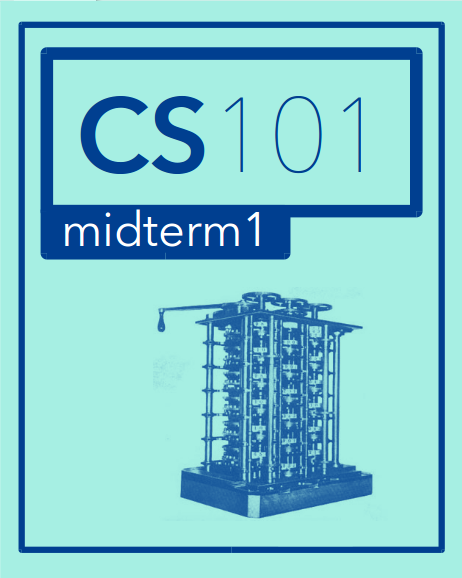
\includegraphics[width=2in]{../img/midterm1-header.png}
\end{center}

\bigskip
\noindent
\begin{itemize}
\item \textbf{Be sure to enter your \underline{NetID} and \underline{the code below} on your Scantron}.
\item Do not turn this page until instructed to do so.
\item There are 30 questions, worth 1 point each.
\item Each question has only \textbf{one} correct answer.
\item You must not communicate with other students during this test.
\item No books, notes, or electronic devices are permitted.
\item This is a 60-minute exam.
\item There are several different versions of this exam.
\end{itemize}

\bigskip\bigskip
\noindent
\textbf{\Large 1. Fill in your information:}

\bigskip
{\Large\bf
\begin{tabular}{ll}
Full Name: & \underbar{\hskip 8cm} \\[0.5em]
UIN (Student Number): & \underbar{\hskip 8cm} \\[0.5em]
NetID: & \underbar{\hskip 8cm}
\end{tabular}
}

\bigskip
\bigskip
\noindent
\textbf{\Large 2. Fill in the following answers on the Scantron form:}

%%%%%%%%%%%%%%%%%%%%%%%%%%%%%%%%%%%%%%%%%%%%%%%%%%%%%%%%%
%%%%%%%%%%%%%%%%%%%%%%%%%%%%%%%%%%%%%%%%%%%%%%%%%%%%%%%%%

\begin{enumerate}
\item[92.] B
\item[93.] B
\item[94.] A
\item[95.] A
\item[96.] A
\end{enumerate}

\newpage

% Zone 1


%%%%%%%%%%%%%%%%%%%%%%%%%%%%%%%%%%%%%%%%%%%%%%%%%%%%%%%%%



\newpage
\noindent
1. (1 point)
How can the following mathematical equation be implemented as a Python expression? Assume \verb|a|, \verb|b|, and \verb|sin| have already been defined.
$$a \sin(a^b - b)$$


\begin{enumerate}
\item[(A)]
\begin{verbatim}a sin(a**b - b)\end{verbatim}

\item[(B)]
\begin{verbatim}a*sin(b^a - b)\end{verbatim}

\item[(C)] $\bigstar$ 
\begin{verbatim}a*sin(a**b - b)\end{verbatim}

\item[(D)]
\begin{verbatim}a*sin(a^b - b)\end{verbatim}

\item[(E)]
None of the other answers are correct.

\end{enumerate}

\vspace*{2em}
\hrule
\vspace{2em}

\noindent {\bf Solution.} 
\vspace{2em}
\hrule height 2pt


\newpage
\noindent
2. (1 point)
Consider the following program:
\begin{verbatim}
x=str("1"*3)
\end{verbatim}
What is the \textbf{value} of \texttt{x} after this program is executed?


\begin{enumerate}
\item[(A)]
\begin{verbatim}"3"\end{verbatim}

\item[(B)]
None of the other answers are correct.

\item[(C)]
\begin{verbatim}3\end{verbatim}

\item[(D)]
\begin{verbatim}111\end{verbatim}

\item[(E)] $\bigstar$ 
\begin{verbatim}"111"\end{verbatim}

\end{enumerate}

\vspace*{2em}
\hrule
\vspace{2em}

\noindent {\bf Solution.} 
\vspace{2em}
\hrule height 2pt


\newpage
\noindent
3. (1 point)
Consider the following program:
\begin{verbatim}
x=[1,2,3]
def f(a):
    s=""
    a.reverse()
    for i in a:
        s+=str(i)
    return s

x.append(f(x))
\end{verbatim}
What is the \textbf{value} of \texttt{x} after this program is executed?


\begin{enumerate}
\item[(A)]
\begin{verbatim}[1, 2, 3]\end{verbatim}

\item[(B)]
\begin{verbatim}[1, 2, 3, '321']\end{verbatim}

\item[(C)]
\begin{verbatim}[3, 2, 1]\end{verbatim}

\item[(D)] $\bigstar$ 
\begin{verbatim}[3, 2, 1, '321']\end{verbatim}

\item[(E)]
\begin{verbatim}[1, 2, 3, 6]\end{verbatim}

\end{enumerate}

\vspace*{2em}
\hrule
\vspace{2em}

\noindent {\bf Solution.} 
\vspace{2em}
\hrule height 2pt


\newpage
\noindent
4. (1 point)
Consider the following incomplete function.
\begin{verbatim}
def isdivisible(m,n):
    if ???:
        return False
    else:
        return True
\end{verbatim}
The function is intended to return True if the input parameter m is evenly divisible by the parameter n and False otherwise. For example, \verb|isdivisible(4,2)| should return \verb|True|, but \verb|isdivisible(5,3)| should return \verb|False|. What should replace the three question marks to complete the function?


\begin{enumerate}
\item[(A)]
\begin{verbatim}(n % m) == 0 \end{verbatim}

\item[(B)]
\begin{verbatim}(n // m) == 0 \end{verbatim}

\item[(C)]
\begin{verbatim}(m // n) != 0 \end{verbatim}

\item[(D)] $\bigstar$ 
\begin{verbatim}(m % n) != 0 \end{verbatim}

\end{enumerate}

\vspace*{2em}
\hrule
\vspace{2em}

\noindent {\bf Solution.} 
\vspace{2em}
\hrule height 2pt


\newpage
\noindent
5. (1 point)
Consider the following program.
\begin{verbatim}
x=0
i=1
while(i*i)<=9:
    x=x+(i*i)
    i=i+1
\end{verbatim}
After it is run, what is the final \textbf{value} of \texttt{x}?


\begin{enumerate}
\item[(A)]
\begin{verbatim}30\end{verbatim}

\item[(B)]
\begin{verbatim}4\end{verbatim}

\item[(C)]
\begin{verbatim}3\end{verbatim}

\item[(D)] $\bigstar$ 
\begin{verbatim}14\end{verbatim}

\item[(E)]
\begin{verbatim}5\end{verbatim}

\end{enumerate}

\vspace*{2em}
\hrule
\vspace{2em}

\noindent {\bf Solution.} 
\vspace{2em}
\hrule height 2pt


\newpage
\noindent
6. (1 point)
Consider the following program:
\begin{verbatim}
s="Hobbes"
i=0
x=-1
while i<len(s):
    if s[i]=='b':
        x=i
    i+=1
\end{verbatim}
What is the \textbf{value} of \texttt{x} after this program is executed?


\begin{enumerate}
\item[(A)] $\bigstar$ 
\begin{verbatim}3\end{verbatim}

\item[(B)]
\begin{verbatim}2\end{verbatim}

\item[(C)]
\begin{verbatim}4\end{verbatim}

\item[(D)]
\begin{verbatim}-1\end{verbatim}

\item[(E)]
\begin{verbatim}5\end{verbatim}

\end{enumerate}

\vspace*{2em}
\hrule
\vspace{2em}

\noindent {\bf Solution.} 
\vspace{2em}
\hrule height 2pt


\newpage
\noindent
7. (1 point)
Consider the following incomplete program.
\begin{verbatim}
sum=0
for i in range(0,100):
    ???

\end{verbatim}
The program is intended to sum all of the integers between 1 and 100 (inclusive). What should replace the three question marks to complete the program?


\begin{enumerate}
\item[(A)]
\begin{verbatim}sum=sum+i \end{verbatim}

\item[(B)]
\begin{verbatim}sum+1=sum \end{verbatim}

\item[(C)] $\bigstar$ 
\begin{verbatim}sum=sum+i+1 \end{verbatim}

\item[(D)]
\begin{verbatim}sum=sum+1\end{verbatim}

\end{enumerate}

\vspace*{2em}
\hrule
\vspace{2em}

\noindent {\bf Solution.} 
\vspace{2em}
\hrule height 2pt


\newpage
\noindent
8. (1 point)
Consider the following program:
\begin{verbatim}
a=["S","T","U","P","E","F","Y"]
a=a[0:4]
a.sort()
x=""
for e in a:
    x=e+x
\end{verbatim}
What is the \textbf{value} of \texttt{x} after this program is executed?


\begin{enumerate}
\item[(A)]
None of the other answers are correct.

\item[(B)]
\begin{verbatim}"STUP"\end{verbatim}

\item[(C)] $\bigstar$ 
\begin{verbatim}"UTSP"\end{verbatim}

\item[(D)]
\begin{verbatim}"PUST"\end{verbatim}

\item[(E)]
\begin{verbatim}"PSTU"\end{verbatim}

\end{enumerate}

\vspace*{2em}
\hrule
\vspace{2em}

\noindent {\bf Solution.} 
\vspace{2em}
\hrule height 2pt


\newpage
\noindent
9. (1 point)
Consider the following program:
\begin{verbatim}
x=2
a=6
if (a%3)==2:
    x=x**3
elif(a%3)==1:
    x=x**2
else:
    x=x**1
\end{verbatim}
What is the \textbf{value} of \texttt{x} after this program is executed?


\begin{enumerate}
\item[(A)] $\bigstar$ 
\begin{verbatim}2\end{verbatim}

\item[(B)]
\begin{verbatim}4\end{verbatim}

\item[(C)]
\begin{verbatim}8\end{verbatim}

\item[(D)]
\begin{verbatim}16\end{verbatim}

\item[(E)]
None of the other answers are correct.

\end{enumerate}

\vspace*{2em}
\hrule
\vspace{2em}

\noindent {\bf Solution.} 
\vspace{2em}
\hrule height 2pt


\newpage
\noindent
10. (1 point)
Consider the following Python program.
\begin{verbatim}
e=[1,3,5,7,9,11]
d=[0,0,0]
for i in range(0,len(e)):
    d[i%3]+=e[i]
x=d[1]
\end{verbatim}
After it is run, what is the final \textbf{value} of \texttt{x}?


\begin{enumerate}
\item[(A)] $\bigstar$ 
\begin{verbatim}12\end{verbatim}

\item[(B)]
\begin{verbatim}3\end{verbatim}

\item[(C)]
\begin{verbatim}0\end{verbatim}

\item[(D)]
\begin{verbatim}16\end{verbatim}

\item[(E)]
\begin{verbatim}8\end{verbatim}

\end{enumerate}

\vspace*{2em}
\hrule
\vspace{2em}

\noindent {\bf Solution.} 
\vspace{2em}
\hrule height 2pt


\newpage
\noindent
11. (1 point)
Consider the following program.
\begin{verbatim}
s="ABCBA"
x=0
y=len(s)-1
while s[x]==s[y] and x<=y:
    x+=1
    y-=1
\end{verbatim}
After it is run, what is the final \textbf{value} of \texttt{x}?


\begin{enumerate}
\item[(A)]
\begin{verbatim}2\end{verbatim}

\item[(B)] $\bigstar$ 
\begin{verbatim}3\end{verbatim}

\item[(C)]
\begin{verbatim}4\end{verbatim}

\item[(D)]
\begin{verbatim}1\end{verbatim}

\item[(E)]
\begin{verbatim}0\end{verbatim}

\end{enumerate}

\vspace*{2em}
\hrule
\vspace{2em}

\noindent {\bf Solution.} 
\vspace{2em}
\hrule height 2pt


\newpage
\noindent
12. (1 point)
Consider the following program:
\begin{verbatim}
x=[2,3,4,5,6,7,8,9]
x=x[2:-2]
i=1
while i <= 3:
    x[i]+=1
    i+=1
\end{verbatim}
What is the \textbf{value} of \texttt{x} after this program is executed?


\begin{enumerate}
\item[(A)]
\begin{verbatim}[4, 6, 7, 7]\end{verbatim}

\item[(B)]
\begin{verbatim}[4, 6, 7]\end{verbatim}

\item[(C)] $\bigstar$ 
\begin{verbatim}[4, 6, 7, 8]\end{verbatim}

\item[(D)]
\begin{verbatim}[2, 4, 6, 6]\end{verbatim}

\item[(E)]
\begin{verbatim}[3, 4, 6, 7, 8]\end{verbatim}

\end{enumerate}

\vspace*{2em}
\hrule
\vspace{2em}

\noindent {\bf Solution.} 
\vspace{2em}
\hrule height 2pt


\newpage
\noindent
13. (1 point)
Consider the following program:
\begin{verbatim}
s="-B-O-R-S-"
x=s.split("-")[2:-2]
\end{verbatim}
What is the \textbf{value} of \texttt{x} after this program is executed?


\begin{enumerate}
\item[(A)]
\begin{verbatim}False\end{verbatim}

\item[(B)]
\begin{verbatim}'ORS'\end{verbatim}

\item[(C)]
\begin{verbatim}''\end{verbatim}

\item[(D)] $\bigstar$ 
\begin{verbatim}['O', 'R']\end{verbatim}

\item[(E)]
\begin{verbatim}None\end{verbatim}

\end{enumerate}

\vspace*{2em}
\hrule
\vspace{2em}

\noindent {\bf Solution.} 
\vspace{2em}
\hrule height 2pt


\newpage
\noindent
14. (1 point)
Consider the following program:
\begin{verbatim}
def fix(s):
    a=list(s)
    a.sort()
    return ''.join(a)

x=["one","two","eleven","twelve"]
s1=fix(x[0]+x[-1])
s2=fix(x[1]+x[-2])

if s1<s2:
    x.sort()
elif s1==s2:
    x.reverse()
else:
    x.append("six")
\end{verbatim}
What is the \textbf{value} of \texttt{x} after this program is executed?


\begin{enumerate}
\item[(A)] $\bigstar$ 
\begin{verbatim}['twelve', 'eleven', 'two', 'one']\end{verbatim}

\item[(B)]
\begin{verbatim}['eleven', 'one', 'twelve', 'two']\end{verbatim}

\item[(C)]
\begin{verbatim}['one', 'two', 'eleven', 'twelve', 'six']\end{verbatim}

\item[(D)]
\begin{verbatim}['one', 'two', 'eleven', 'twelve']\end{verbatim}

\item[(E)]
\begin{verbatim}['two', 'twelve', 'one', 'eleven', 'six']\end{verbatim}

\end{enumerate}

\vspace*{2em}
\hrule
\vspace{2em}

\noindent {\bf Solution.} 
\vspace{2em}
\hrule height 2pt


\newpage
\noindent
15. (1 point)
Consider the following program:
\begin{verbatim}
x="KING ARTHUR-MORGANA LEFAY-SIR BEDIVERE".split("-")
y=x
x=y.reverse()
\end{verbatim}
What is the \textbf{value} of \texttt{x} after this program is executed?


\begin{enumerate}
\item[(A)]
\begin{verbatim}['SIR BEDIVERE', 'MORGANA LEFAY', 'KING ARTHUR']\end{verbatim}

\item[(B)]
\begin{verbatim}['KING', 'ARTHUR-MORGANA', 'LEFAY-SIR', 'BEDIVERE']\end{verbatim}

\item[(C)]
\begin{verbatim}['BEDIVERE', 'LEFAY-SIR', 'ARTHUR-MORGANA', 'KING']\end{verbatim}

\item[(D)] $\bigstar$ 
\begin{verbatim}None\end{verbatim}

\item[(E)]
\begin{verbatim}['KING ARTHUR', 'MORGANA LEFAY', 'SIR BEDIVERE']\end{verbatim}

\end{enumerate}

\vspace*{2em}
\hrule
\vspace{2em}

\noindent {\bf Solution.} 
\vspace{2em}
\hrule height 2pt


\newpage
\noindent
16. (1 point)
Evaluate the following expression:
\begin{verbatim}
len("ABCD"[0:3])
\end{verbatim}
What value is produced?


\begin{enumerate}
\item[(A)]
2

\item[(B)]
1

\item[(C)] $\bigstar$ 
3

\item[(D)]
4

\end{enumerate}

\vspace*{2em}
\hrule
\vspace{2em}

\noindent {\bf Solution.} 
\vspace{2em}
\hrule height 2pt


\newpage
\noindent
17. (1 point)
Consider the following program:
\begin{verbatim}
pi="3.14159"
e="2.71828"
x=pi in pi*len(e)
\end{verbatim}
What is the \textbf{type} of \texttt{x} after this program is executed?


\begin{enumerate}
\item[(A)]
\begin{verbatim}None\end{verbatim}

\item[(B)]
\begin{verbatim}Float\end{verbatim}

\item[(C)]
\begin{verbatim}Integer\end{verbatim}

\item[(D)]
\begin{verbatim}String\end{verbatim}

\item[(E)] $\bigstar$ 
\begin{verbatim}Boolean\end{verbatim}

\end{enumerate}

\vspace*{2em}
\hrule
\vspace{2em}

\noindent {\bf Solution.} 
\vspace{2em}
\hrule height 2pt


\newpage
\noindent
18. (1 point)
Consider the following program:
\begin{verbatim}
x=0
for i in range(2,8):
    if i%3==0:
        x+=3
    elif i%2==0:
        x+=2
    else:
        x+=1
\end{verbatim}
What is the \textbf{value} of \texttt{x} after this program is executed?


\begin{enumerate}
\item[(A)]
\begin{verbatim}11\end{verbatim}

\item[(B)] $\bigstar$ 
\begin{verbatim}12\end{verbatim}

\item[(C)]
\begin{verbatim}10\end{verbatim}

\item[(D)]
\begin{verbatim}13\end{verbatim}

\item[(E)]
\begin{verbatim}14\end{verbatim}

\end{enumerate}

\vspace*{2em}
\hrule
\vspace{2em}

\noindent {\bf Solution.} 
\vspace{2em}
\hrule height 2pt


\newpage
\noindent
19. (1 point)
Consider the following program:
\begin{verbatim}
s="TRIS %i"
t="ISEU"
x=len(s) % len(t[2:-1])
\end{verbatim}
What is the \textbf{type} of \texttt{x} after this program is executed?


\begin{enumerate}
\item[(A)]
\begin{verbatim}None\end{verbatim}

\item[(B)]
\begin{verbatim}Boolean\end{verbatim}

\item[(C)]
\begin{verbatim}String\end{verbatim}

\item[(D)]
\begin{verbatim}Float\end{verbatim}

\item[(E)] $\bigstar$ 
\begin{verbatim}Integer\end{verbatim}

\end{enumerate}

\vspace*{2em}
\hrule
\vspace{2em}

\noindent {\bf Solution.} 
\vspace{2em}
\hrule height 2pt


\newpage
\noindent
20. (1 point)
Consider the following program.
\begin{verbatim}
kay = 2
wart = 3

def knight(kay,wart):
    wart += 2
    kay += 3
    return wart + kay

wart = knight(kay, kay) + knight(wart, wart)
\end{verbatim}
After it is run, what is the final \textbf{value} of \texttt{wart}?


\begin{enumerate}
\item[(A)]
\begin{verbatim}3\end{verbatim}

\item[(B)]
\begin{verbatim}5\end{verbatim}

\item[(C)] $\bigstar$ 
None of the other answers are correct.

\item[(D)]
\begin{verbatim}2\end{verbatim}

\end{enumerate}

\vspace*{2em}
\hrule
\vspace{2em}

\noindent {\bf Solution.} 
\vspace{2em}
\hrule height 2pt


\newpage
\noindent
21. (1 point)
Consider the following program:
\begin{verbatim}
a=3
b=4
if a!=b:
    a=b
elif a==4:
    a=5
else:
    b=a
\end{verbatim}
What is the \textbf{value} of a after this program is executed?


\begin{enumerate}
\item[(A)]
\begin{verbatim}5\end{verbatim}

\item[(B)]
\begin{verbatim}7\end{verbatim}

\item[(C)] $\bigstar$ 
\begin{verbatim}4\end{verbatim}

\item[(D)]
None of the other answers are correct.

\item[(E)]
\begin{verbatim}3\end{verbatim}

\end{enumerate}

\vspace*{2em}
\hrule
\vspace{2em}

\noindent {\bf Solution.} 
\vspace{2em}
\hrule height 2pt


\newpage
\noindent
22. (1 point)
Consider the following program:
\begin{verbatim}
s="ECTOR"
t="GAWAIN"
x=(len(s)/(len(t)-1))+1
\end{verbatim}
What is the \textbf{type} of \texttt{x} after this program is executed?


\begin{enumerate}
\item[(A)]
\begin{verbatim}Integer\end{verbatim}

\item[(B)]
\begin{verbatim}None\end{verbatim}

\item[(C)]
\begin{verbatim}Boolean\end{verbatim}

\item[(D)] $\bigstar$ 
\begin{verbatim}Float\end{verbatim}

\item[(E)]
\begin{verbatim}String\end{verbatim}

\end{enumerate}

\vspace*{2em}
\hrule
\vspace{2em}

\noindent {\bf Solution.} 
\vspace{2em}
\hrule height 2pt


\newpage
\noindent
23. (1 point)
Consider the following program.
\begin{verbatim}
x=[]
for j in range(0,5):
    if (j%2)==0:
        x.append("-")
    if (j%5)==0:
        x.append("*")
\end{verbatim}
After it is run, what is the final \textbf{value} of \texttt{x}?


\begin{enumerate}
\item[(A)]
None of the other answers are correct.

\item[(B)]
\begin{verbatim}["-","-","*"]\end{verbatim}

\item[(C)]
\begin{verbatim}["-","*","-"]\end{verbatim}

\item[(D)] $\bigstar$ 
\begin{verbatim}["-","*","-","-"]\end{verbatim}

\item[(E)]
\begin{verbatim}["*","-","*","*"]\end{verbatim}

\end{enumerate}

\vspace*{2em}
\hrule
\vspace{2em}

\noindent {\bf Solution.} 
\vspace{2em}
\hrule height 2pt


\newpage
\noindent
24. (1 point)
What is the result of the following expression?
\begin{verbatim}
[ 1, 2, 3 ] * 3
\end{verbatim}


\begin{enumerate}
\item[(A)] $\bigstar$ 
\begin{verbatim}[1, 2, 3, 1, 2, 3, 1, 2, 3]\end{verbatim}

\item[(B)]
\begin{verbatim}(3, 6, 9)\end{verbatim}

\item[(C)]
\begin{verbatim}[1.0, 2.0, 3.0, 1.0, 2.0, 3.0, 1.0, 2.0, 3.0]\end{verbatim}

\item[(D)]
\begin{verbatim}[3, 6, 9]\end{verbatim}

\item[(E)]
\begin{verbatim}[3.0, 6.0, 9.0]\end{verbatim}

\end{enumerate}

\vspace*{2em}
\hrule
\vspace{2em}

\noindent {\bf Solution.} 
\vspace{2em}
\hrule height 2pt


\newpage
\noindent
25. (1 point)
Consider the following program:
\begin{verbatim}
a=["merlin","sir agravaine","king pellinore"]
b=[ ]
for i in range(0,4):
    b.append(a[0-i].title())
\end{verbatim}
What is the \textbf{value} of b after this program is executed?


\begin{enumerate}
\item[(A)]
\begin{verbatim}['Merlin', 'King Pellinore', 'Sir Agravaine']\end{verbatim}

\item[(B)] $\bigstar$ 
\begin{verbatim}['Merlin', 'King Pellinore', 'Sir Agravaine', 'Merlin']\end{verbatim}

\item[(C)]
\begin{verbatim}[ ]\end{verbatim}

\item[(D)]
\begin{verbatim}['Merlin', 'Sir Agravaine', 'King Pellinore', 'Merlin']\end{verbatim}

\item[(E)]
\begin{verbatim}['King Pellinore', 'Sir Agravaine', 'Merlin']\end{verbatim}

\end{enumerate}

\vspace*{2em}
\hrule
\vspace{2em}

\noindent {\bf Solution.} 
\vspace{2em}
\hrule height 2pt


\newpage
\noindent
26. (1 point)
Consider the following incomplete Python program.
\begin{verbatim}
s="".join(["1","0","2","1"])
x=0
for i in range(len(s)-1):
    x+=int(???)
\end{verbatim}
What should replace the three question marks so the resulting value of \texttt{x} is 33?


\begin{enumerate}
\item[(A)]
\begin{verbatim}s[i:i-1]\end{verbatim}

\item[(B)]
\begin{verbatim}s[i+1:i+2]\end{verbatim}

\item[(C)] $\bigstar$ 
\begin{verbatim}s[i:i+2]\end{verbatim}

\item[(D)]
\begin{verbatim}s[i:i+1]\end{verbatim}

\end{enumerate}

\vspace*{2em}
\hrule
\vspace{2em}

\noindent {\bf Solution.} 
\vspace{2em}
\hrule height 2pt


\newpage
\noindent
27. (1 point)
Consider the following program.
\begin{verbatim}
def artificing(s):
    return s*2
    return s+"%i" % 2
    return s

s=artificing("MERLIN")
\end{verbatim}
After it is run, what is the final \textbf{value} of s?


\begin{enumerate}
\item[(A)]
\begin{verbatim}"MERLIN"\end{verbatim}

\item[(B)] $\bigstar$ 
\begin{verbatim}"MERLINMERLIN"\end{verbatim}

\item[(C)]
\begin{verbatim}12\end{verbatim}

\item[(D)]
\begin{verbatim}"MERLIN2"\end{verbatim}

\item[(E)]
\begin{verbatim}None\end{verbatim}

\end{enumerate}

\vspace*{2em}
\hrule
\vspace{2em}

\noindent {\bf Solution.} 
\vspace{2em}
\hrule height 2pt


\newpage
\noindent
28. (1 point)
For this problem, you should compose a function which accomplishes a given task using the available code blocks arranged in the correct functional order.  \emph{We ignore indentation for this problem.}

\texttt{find\_max} should accept a \texttt{list} and return the value of the maximum item in the \texttt{list}.  (\texttt{None} is always the lowest value in any numeric comparison, so you may use it as an initializer.)

\begin{verbatim}
def find_max(my_list):
\end{verbatim}

\begin{enumerate}[1]
\item \texttt{max\_val = i}
\item \texttt{max\_val = None}
\item \texttt{for i in range(len(my\_list)):}
\item \texttt{if i > max\_val:}
\item \texttt{max\_val = my\_list[i]}
\item \texttt{return max\_val}
\item \texttt{for i in range(my\_list):}
\item \texttt{if my\_list[i] > max\_val:}
\item \texttt{print(max\_val)}
\end{enumerate}



\begin{enumerate}
\item[(A)]
2, 3, 8, 1, 6

\item[(B)]
2, 7, 4, 5, 6

\item[(C)] $\bigstar$ 
2, 3, 8, 5, 6

\item[(D)]
3, 2, 8, 5, 9

\item[(E)]
2, 3, 4, 1, 6

\end{enumerate}

\vspace*{2em}
\hrule
\vspace{2em}

\noindent {\bf Solution.} 
\vspace{2em}
\hrule height 2pt


\newpage
\noindent
29. (1 point)
Evaluate the following expression:
\begin{verbatim}
[1,2]*len("3")
\end{verbatim}
What value is produced?


\begin{enumerate}
\item[(A)] $\bigstar$ 
\begin{verbatim}[1,2]\end{verbatim}

\item[(B)]
\begin{verbatim}[1,2,1]\end{verbatim}

\item[(C)]
\begin{verbatim}[1,2,1,2,1,2]\end{verbatim}

\item[(D)]
\begin{verbatim}[1,2,3]\end{verbatim}

\end{enumerate}

\vspace*{2em}
\hrule
\vspace{2em}

\noindent {\bf Solution.} 
\vspace{2em}
\hrule height 2pt


\newpage
\noindent
30. (1 point)
Consider the following program:
\begin{verbatim}
i=2
x=3
while i < 7:
    x+=i
    i+=2
\end{verbatim}
What is the \textbf{value} of \texttt{x} after this program is executed?


\begin{enumerate}
\item[(A)]
\begin{verbatim}12\end{verbatim}

\item[(B)]
\begin{verbatim}11\end{verbatim}

\item[(C)]
\begin{verbatim}13\end{verbatim}

\item[(D)] $\bigstar$ 
\begin{verbatim}15\end{verbatim}

\item[(E)]
\begin{verbatim}14\end{verbatim}

\end{enumerate}

\vspace*{2em}
\hrule
\vspace{2em}

\noindent {\bf Solution.} 
\vspace{2em}
\hrule height 2pt

%%%%%%%%%%%%%%%%%%%%%%%%%%%%%%%%%%%%%%%%%%%%%%%%%%%%%%%%%%%%%%%%%%%%%%
%%%%%%%%%%%%%%%%%%%%%%%%%%%%%%%%%%%%%%%%%%%%%%%%%%%%%%%%%%%%%%%%%%%%%%
%%%%%%%%%%%%%%%%%%%%%%%%%%%%%%%%%%%%%%%%%%%%%%%%%%%%%%%%%%%%%%%%%%%%%%
%%%%%%%%%%%%%%%%%%%%%%%%%%%%%%%%%%%%%%%%%%%%%%%%%%%%%%%%%%%%%%%%%%%%%%
% Exam number 8

\message{Exam 8/50}
\cleardoublepage
\setcounter{page}{1}


\begin{center}
%\textbf{\Large CS 101 Midterm \#1}
%
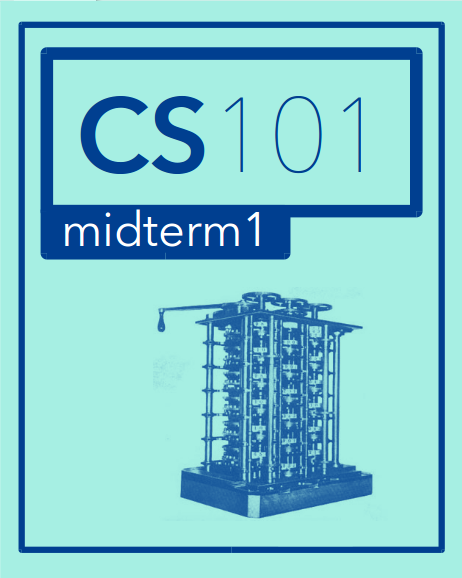
\includegraphics[width=2in]{../img/midterm1-header.png}
\end{center}

\bigskip
\noindent
\begin{itemize}
\item \textbf{Be sure to enter your \underline{NetID} and \underline{the code below} on your Scantron}.
\item Do not turn this page until instructed to do so.
\item There are 30 questions, worth 1 point each.
\item Each question has only \textbf{one} correct answer.
\item You must not communicate with other students during this test.
\item No books, notes, or electronic devices are permitted.
\item This is a 60-minute exam.
\item There are several different versions of this exam.
\end{itemize}

\bigskip\bigskip
\noindent
\textbf{\Large 1. Fill in your information:}

\bigskip
{\Large\bf
\begin{tabular}{ll}
Full Name: & \underbar{\hskip 8cm} \\[0.5em]
UIN (Student Number): & \underbar{\hskip 8cm} \\[0.5em]
NetID: & \underbar{\hskip 8cm}
\end{tabular}
}

\bigskip
\bigskip
\noindent
\textbf{\Large 2. Fill in the following answers on the Scantron form:}

%%%%%%%%%%%%%%%%%%%%%%%%%%%%%%%%%%%%%%%%%%%%%%%%%%%%%%%%%
%%%%%%%%%%%%%%%%%%%%%%%%%%%%%%%%%%%%%%%%%%%%%%%%%%%%%%%%%

\begin{enumerate}
\item[92.] C
\item[93.] B
\item[94.] A
\item[95.] B
\item[96.] B
\end{enumerate}

\newpage

% Zone 1


%%%%%%%%%%%%%%%%%%%%%%%%%%%%%%%%%%%%%%%%%%%%%%%%%%%%%%%%%



\newpage
\noindent
1. (1 point)
Consider the following incomplete program.
\begin{verbatim}
sum=0
???:
    sum=sum+i

\end{verbatim}
The program is intended to sum all of the integers between 1 and 100 (inclusive). What should replace the three question marks to complete the program?


\begin{enumerate}
\item[(A)]
\begin{verbatim}while i<=100 \end{verbatim}

\item[(B)] $\bigstar$ 
\begin{verbatim}for i in range(1,101) \end{verbatim}

\item[(C)]
\begin{verbatim}while i in range(100)\end{verbatim}

\item[(D)]
\begin{verbatim}for i in range(0,100)\end{verbatim}

\end{enumerate}

\vspace*{2em}
\hrule
\vspace{2em}

\noindent {\bf Solution.} 
\vspace{2em}
\hrule height 2pt


\newpage
\noindent
2. (1 point)
Evaluate the following expression:
\begin{verbatim}
len("ABCDE"[1:4])
\end{verbatim}
What value is produced?


\begin{enumerate}
\item[(A)]
1

\item[(B)]
5

\item[(C)]
4

\item[(D)] $\bigstar$ 
3

\end{enumerate}

\vspace*{2em}
\hrule
\vspace{2em}

\noindent {\bf Solution.} 
\vspace{2em}
\hrule height 2pt


\newpage
\noindent
3. (1 point)
Consider the following program:
\begin{verbatim}
x=0
for i in range(2,8):
    if i%3==0:
        x+=3
    elif i%2==0:
        x+=2
    else:
        x+=1
\end{verbatim}
What is the \textbf{value} of \texttt{x} after this program is executed?


\begin{enumerate}
\item[(A)]
\begin{verbatim}11\end{verbatim}

\item[(B)] $\bigstar$ 
\begin{verbatim}12\end{verbatim}

\item[(C)]
\begin{verbatim}13\end{verbatim}

\item[(D)]
\begin{verbatim}14\end{verbatim}

\item[(E)]
\begin{verbatim}10\end{verbatim}

\end{enumerate}

\vspace*{2em}
\hrule
\vspace{2em}

\noindent {\bf Solution.} 
\vspace{2em}
\hrule height 2pt


\newpage
\noindent
4. (1 point)
Evaluate the following expression:
\begin{verbatim}
[1,2]*len("3")
\end{verbatim}
What value is produced?


\begin{enumerate}
\item[(A)]
\begin{verbatim}[1,2,1,2,1,2]\end{verbatim}

\item[(B)] $\bigstar$ 
\begin{verbatim}[1,2]\end{verbatim}

\item[(C)]
\begin{verbatim}[1,2,3]\end{verbatim}

\item[(D)]
\begin{verbatim}[1,2,1]\end{verbatim}

\end{enumerate}

\vspace*{2em}
\hrule
\vspace{2em}

\noindent {\bf Solution.} 
\vspace{2em}
\hrule height 2pt


\newpage
\noindent
5. (1 point)
Consider the following Python program.
\begin{verbatim}
e=[1,3,5,7,9,11]
d=[0,0,0]
for i in range(0,len(e)):
    d[i%3]+=e[i]
x=d[2]
\end{verbatim}
After it is run, what is the final \textbf{value} of \texttt{x}?


\begin{enumerate}
\item[(A)] $\bigstar$ 
\begin{verbatim}16\end{verbatim}

\item[(B)]
\begin{verbatim}7\end{verbatim}

\item[(C)]
\begin{verbatim}8\end{verbatim}

\item[(D)]
\begin{verbatim}0\end{verbatim}

\item[(E)]
\begin{verbatim}12\end{verbatim}

\end{enumerate}

\vspace*{2em}
\hrule
\vspace{2em}

\noindent {\bf Solution.} 
\vspace{2em}
\hrule height 2pt


\newpage
\noindent
6. (1 point)
Consider the following program.
\begin{verbatim}
kay = 2
wart = 3

def knight(kay,wart):
    wart += 2
    kay += 3
    return wart + kay

kay = knight(wart, kay) + knight(kay, wart)
\end{verbatim}
After it is run, what is the final \textbf{value} of \texttt{kay}?


\begin{enumerate}
\item[(A)]
\begin{verbatim}2\end{verbatim}

\item[(B)] $\bigstar$ 
None of the other answers are correct.

\item[(C)]
\begin{verbatim}5\end{verbatim}

\item[(D)]
\begin{verbatim}3\end{verbatim}

\end{enumerate}

\vspace*{2em}
\hrule
\vspace{2em}

\noindent {\bf Solution.} 
\vspace{2em}
\hrule height 2pt


\newpage
\noindent
7. (1 point)
Consider the following program.
\begin{verbatim}
x=0
i=1
while(i*i)<=9:
    x=x+(i*i)
    i=i+1
\end{verbatim}
After it is run, what is the final \textbf{value} of \texttt{x}?


\begin{enumerate}
\item[(A)]
\begin{verbatim}4\end{verbatim}

\item[(B)] $\bigstar$ 
\begin{verbatim}14\end{verbatim}

\item[(C)]
\begin{verbatim}30\end{verbatim}

\item[(D)]
\begin{verbatim}3\end{verbatim}

\item[(E)]
\begin{verbatim}5\end{verbatim}

\end{enumerate}

\vspace*{2em}
\hrule
\vspace{2em}

\noindent {\bf Solution.} 
\vspace{2em}
\hrule height 2pt


\newpage
\noindent
8. (1 point)
Consider the following program:
\begin{verbatim}
s="G+R+A+I+L"
x=s.split("+")[1:-2]
\end{verbatim}
What is the \textbf{value} of \texttt{x} after this program is executed?


\begin{enumerate}
\item[(A)] $\bigstar$ 
\begin{verbatim}['R','A']\end{verbatim}

\item[(B)]
\begin{verbatim}3\end{verbatim}

\item[(C)]
\begin{verbatim}'RAI'\end{verbatim}

\item[(D)]
\begin{verbatim}None\end{verbatim}

\item[(E)]
\begin{verbatim}False\end{verbatim}

\end{enumerate}

\vspace*{2em}
\hrule
\vspace{2em}

\noindent {\bf Solution.} 
\vspace{2em}
\hrule height 2pt


\newpage
\noindent
9. (1 point)
Consider the following program.
\begin{verbatim}
s="ABCBA"
x=0
y=len(s)-1
while s[x]==s[y] and x<=y:
    x+=1
    y-=1
\end{verbatim}
After it is run, what is the final \textbf{value} of \texttt{x}?


\begin{enumerate}
\item[(A)] $\bigstar$ 
\begin{verbatim}3\end{verbatim}

\item[(B)]
\begin{verbatim}2\end{verbatim}

\item[(C)]
\begin{verbatim}4\end{verbatim}

\item[(D)]
\begin{verbatim}0\end{verbatim}

\item[(E)]
\begin{verbatim}1\end{verbatim}

\end{enumerate}

\vspace*{2em}
\hrule
\vspace{2em}

\noindent {\bf Solution.} 
\vspace{2em}
\hrule height 2pt


\newpage
\noindent
10. (1 point)
Consider the following program:
\begin{verbatim}
s="ECTOR"
t="GAWAIN"
x=(len(s)/(len(t)-1))+1
\end{verbatim}
What is the \textbf{type} of \texttt{x} after this program is executed?


\begin{enumerate}
\item[(A)]
\begin{verbatim}String\end{verbatim}

\item[(B)]
\begin{verbatim}Integer\end{verbatim}

\item[(C)]
\begin{verbatim}None\end{verbatim}

\item[(D)]
\begin{verbatim}Boolean\end{verbatim}

\item[(E)] $\bigstar$ 
\begin{verbatim}Float\end{verbatim}

\end{enumerate}

\vspace*{2em}
\hrule
\vspace{2em}

\noindent {\bf Solution.} 
\vspace{2em}
\hrule height 2pt


\newpage
\noindent
11. (1 point)
Consider the following program:
\begin{verbatim}
def fix(s):
    a=list(s)
    a.sort()
    return ''.join(a)

x=["one","two","eleven","twelve"]
s1=fix(x[0]+x[-1])
s2=fix(x[1]+x[-2])

if s1==s2:
    x.sort()
elif s1<s2:
    x.reverse()
else:
    x.append("six")
\end{verbatim}
What is the \textbf{value} of \texttt{x} after this program is executed?


\begin{enumerate}
\item[(A)]
\begin{verbatim}['two', 'twelve', 'one', 'eleven', 'six']\end{verbatim}

\item[(B)] $\bigstar$ 
\begin{verbatim}['eleven', 'one', 'twelve', 'two']\end{verbatim}

\item[(C)]
\begin{verbatim}['twelve', 'eleven', 'two', 'one']\end{verbatim}

\item[(D)]
\begin{verbatim}['one', 'two', 'eleven', 'twelve']\end{verbatim}

\item[(E)]
\begin{verbatim}['one', 'two', 'eleven', 'twelve', 'six']\end{verbatim}

\end{enumerate}

\vspace*{2em}
\hrule
\vspace{2em}

\noindent {\bf Solution.} 
\vspace{2em}
\hrule height 2pt


\newpage
\noindent
12. (1 point)
Consider the following program.
\begin{verbatim}
x=[]
for j in range(0,5):
    if (j%4)==0:
        x.append("-")
    if (j%5)==0:
        x.append("*")
\end{verbatim}
After it is run, what is the final \textbf{value} of \texttt{x}?


\begin{enumerate}
\item[(A)]
None of the other answers are correct.

\item[(B)]
\begin{verbatim}["-","*","*"]\end{verbatim}

\item[(C)]
\begin{verbatim}["-","-","*"]\end{verbatim}

\item[(D)] $\bigstar$ 
\begin{verbatim}["-","*","-"]\end{verbatim}

\item[(E)]
\begin{verbatim}["-","*"]\end{verbatim}

\end{enumerate}

\vspace*{2em}
\hrule
\vspace{2em}

\noindent {\bf Solution.} 
\vspace{2em}
\hrule height 2pt


\newpage
\noindent
13. (1 point)
Consider the following program:
\begin{verbatim}
s="TRIS %i"
t="ISEU"
x=len(s) % len(t[2:-1])
\end{verbatim}
What is the \textbf{type} of \texttt{x} after this program is executed?


\begin{enumerate}
\item[(A)]
\begin{verbatim}Boolean\end{verbatim}

\item[(B)]
\begin{verbatim}None\end{verbatim}

\item[(C)]
\begin{verbatim}Float\end{verbatim}

\item[(D)]
\begin{verbatim}String\end{verbatim}

\item[(E)] $\bigstar$ 
\begin{verbatim}Integer\end{verbatim}

\end{enumerate}

\vspace*{2em}
\hrule
\vspace{2em}

\noindent {\bf Solution.} 
\vspace{2em}
\hrule height 2pt


\newpage
\noindent
14. (1 point)
Consider the following program:
\begin{verbatim}
a=["merlin","sir agravaine","king pellinore"]
b=[ ]
for i in range(0,4):
    b.append(a[0-i].title())
\end{verbatim}
What is the \textbf{value} of b after this program is executed?


\begin{enumerate}
\item[(A)] $\bigstar$ 
\begin{verbatim}['Merlin', 'King Pellinore', 'Sir Agravaine', 'Merlin']\end{verbatim}

\item[(B)]
\begin{verbatim}[ ]\end{verbatim}

\item[(C)]
\begin{verbatim}['Merlin', 'Sir Agravaine', 'King Pellinore', 'Merlin']\end{verbatim}

\item[(D)]
\begin{verbatim}['Merlin', 'King Pellinore', 'Sir Agravaine']\end{verbatim}

\item[(E)]
\begin{verbatim}['King Pellinore', 'Sir Agravaine', 'Merlin']\end{verbatim}

\end{enumerate}

\vspace*{2em}
\hrule
\vspace{2em}

\noindent {\bf Solution.} 
\vspace{2em}
\hrule height 2pt


\newpage
\noindent
15. (1 point)
Consider the following program.
\begin{verbatim}
def artificing(s):
    return s+"%i" % 2
    return s*2
    return s

s=artificing("MERLIN")
\end{verbatim}
After it is run, what is the final \textbf{value} of s?


\begin{enumerate}
\item[(A)]
\begin{verbatim}"MERLIN%i"\end{verbatim}

\item[(B)]
\begin{verbatim}None\end{verbatim}

\item[(C)] $\bigstar$ 
\begin{verbatim}"MERLIN2"\end{verbatim}

\item[(D)]
\begin{verbatim}0\end{verbatim}

\item[(E)]
\begin{verbatim}"MERLINMERLIN"\end{verbatim}

\end{enumerate}

\vspace*{2em}
\hrule
\vspace{2em}

\noindent {\bf Solution.} 
\vspace{2em}
\hrule height 2pt


\newpage
\noindent
16. (1 point)
Consider the following program:
\begin{verbatim}
x="KING ARTHUR-MORGANA LEFAY-SIR BEDIVERE".split("-")
y=x
x=y.reverse()
\end{verbatim}
What is the \textbf{value} of \texttt{x} after this program is executed?


\begin{enumerate}
\item[(A)]
\begin{verbatim}['BEDIVERE', 'LEFAY-SIR', 'ARTHUR-MORGANA', 'KING']\end{verbatim}

\item[(B)]
\begin{verbatim}['SIR BEDIVERE', 'MORGANA LEFAY', 'KING ARTHUR']\end{verbatim}

\item[(C)]
\begin{verbatim}['KING ARTHUR', 'MORGANA LEFAY', 'SIR BEDIVERE']\end{verbatim}

\item[(D)] $\bigstar$ 
\begin{verbatim}None\end{verbatim}

\item[(E)]
\begin{verbatim}['KING', 'ARTHUR-MORGANA', 'LEFAY-SIR', 'BEDIVERE']\end{verbatim}

\end{enumerate}

\vspace*{2em}
\hrule
\vspace{2em}

\noindent {\bf Solution.} 
\vspace{2em}
\hrule height 2pt


\newpage
\noindent
17. (1 point)
Consider the following program:
\begin{verbatim}
x=[2,3,4,5,6,7,8,9]
x=x[2:-2]
i=1
while i <= 3:
    x[i]+=1
    i+=1
\end{verbatim}
What is the \textbf{value} of \texttt{x} after this program is executed?


\begin{enumerate}
\item[(A)]
\begin{verbatim}[2, 4, 6, 6]\end{verbatim}

\item[(B)]
\begin{verbatim}[4, 6, 7, 7]\end{verbatim}

\item[(C)] $\bigstar$ 
\begin{verbatim}[4, 6, 7, 8]\end{verbatim}

\item[(D)]
\begin{verbatim}[3, 4, 6, 7, 8]\end{verbatim}

\item[(E)]
\begin{verbatim}[4, 6, 7]\end{verbatim}

\end{enumerate}

\vspace*{2em}
\hrule
\vspace{2em}

\noindent {\bf Solution.} 
\vspace{2em}
\hrule height 2pt


\newpage
\noindent
18. (1 point)
Consider the following program:
\begin{verbatim}
x=[1,2,3]
def f(a):
    s=""
    a.reverse()
    for i in a:
        s+=str(i)
    return s

x.append(f(x))
\end{verbatim}
What is the \textbf{value} of \texttt{x} after this program is executed?


\begin{enumerate}
\item[(A)]
\begin{verbatim}[1, 2, 3, '321']\end{verbatim}

\item[(B)]
\begin{verbatim}[1, 2, 3, 6]\end{verbatim}

\item[(C)] $\bigstar$ 
\begin{verbatim}[3, 2, 1, '321']\end{verbatim}

\item[(D)]
\begin{verbatim}[3, 2, 1]\end{verbatim}

\item[(E)]
\begin{verbatim}[1, 2, 3]\end{verbatim}

\end{enumerate}

\vspace*{2em}
\hrule
\vspace{2em}

\noindent {\bf Solution.} 
\vspace{2em}
\hrule height 2pt


\newpage
\noindent
19. (1 point)
Consider the following program:
\begin{verbatim}
a=3
b=4
if a!=b:
    a=b
elif a==4:
    a=5
else:
    b=a
\end{verbatim}
What is the \textbf{value} of a after this program is executed?


\begin{enumerate}
\item[(A)]
\begin{verbatim}3\end{verbatim}

\item[(B)]
None of the other answers are correct.

\item[(C)]
\begin{verbatim}5\end{verbatim}

\item[(D)]
\begin{verbatim}7\end{verbatim}

\item[(E)] $\bigstar$ 
\begin{verbatim}4\end{verbatim}

\end{enumerate}

\vspace*{2em}
\hrule
\vspace{2em}

\noindent {\bf Solution.} 
\vspace{2em}
\hrule height 2pt


\newpage
\noindent
20. (1 point)
Consider the following incomplete function.
\begin{verbatim}
def ismultiple(m,n):
    if ???:
        return False
    else:
        return True
\end{verbatim}
The function is intended to return True if the input parameter m is a multiple of parameter n and False otherwise. For example, \verb|ismultiple(4,2)| should return \verb|True|, but \verb|ismultiple(5,3)| should return \verb|False|. What should replace the three question marks to complete the function?


\begin{enumerate}
\item[(A)]
\begin{verbatim}(n % m) == 0 \end{verbatim}

\item[(B)]
\begin{verbatim}(m // n) != 0 \end{verbatim}

\item[(C)]
\begin{verbatim}(n // m) == 0 \end{verbatim}

\item[(D)] $\bigstar$ 
\begin{verbatim}(m % n) != 0 \end{verbatim}

\end{enumerate}

\vspace*{2em}
\hrule
\vspace{2em}

\noindent {\bf Solution.} 
\vspace{2em}
\hrule height 2pt


\newpage
\noindent
21. (1 point)
For this problem, you should compose a function which accomplishes a given task using the available code blocks arranged in the correct functional order.  \emph{We ignore indentation for this problem.}

\texttt{find\_max} should accept a \texttt{list} and return the value of the maximum item in the \texttt{list}.  (\texttt{None} is always the lowest value in any numeric comparison, so you may use it as an initializer.)

\begin{verbatim}
def find_max(my_list):
\end{verbatim}

\begin{enumerate}[1]
\item \texttt{max\_val = i}
\item \texttt{max\_val = None}
\item \texttt{for i in range(len(my\_list)):}
\item \texttt{if i > max\_val:}
\item \texttt{max\_val = my\_list[i]}
\item \texttt{return max\_val}
\item \texttt{for i in range(my\_list):}
\item \texttt{if my\_list[i] > max\_val:}
\item \texttt{print(max\_val)}
\end{enumerate}



\begin{enumerate}
\item[(A)]
2, 7, 4, 5, 6

\item[(B)] $\bigstar$ 
2, 3, 8, 5, 6

\item[(C)]
2, 3, 8, 1, 6

\item[(D)]
3, 2, 8, 5, 9

\item[(E)]
2, 3, 4, 1, 6

\end{enumerate}

\vspace*{2em}
\hrule
\vspace{2em}

\noindent {\bf Solution.} 
\vspace{2em}
\hrule height 2pt


\newpage
\noindent
22. (1 point)
\begin{verbatim}
x=str(3)+"str(3)"
\end{verbatim}
What is the \textbf{value} of \texttt{x} after this program is executed?


\begin{enumerate}
\item[(A)]
\begin{verbatim}"333"\end{verbatim}

\item[(B)] $\bigstar$ 
\begin{verbatim}"3str(3)"\end{verbatim}

\item[(C)]
\begin{verbatim}33\end{verbatim}

\item[(D)]
None of the other answers are correct.

\item[(E)]
\begin{verbatim}"33"\end{verbatim}

\end{enumerate}

\vspace*{2em}
\hrule
\vspace{2em}

\noindent {\bf Solution.} 
\vspace{2em}
\hrule height 2pt


\newpage
\noindent
23. (1 point)
Consider the following program:
\begin{verbatim}
pi="3.14159"
e="2.71828"
x=(float(e)**float(pi)-float(pi)) == 20
\end{verbatim}
What is the \textbf{type} of \texttt{x} after this program is executed?


\begin{enumerate}
\item[(A)]
\begin{verbatim}None\end{verbatim}

\item[(B)] $\bigstar$ 
\begin{verbatim}Boolean\end{verbatim}

\item[(C)]
\begin{verbatim}String\end{verbatim}

\item[(D)]
\begin{verbatim}Integer\end{verbatim}

\item[(E)]
\begin{verbatim}Float\end{verbatim}

\end{enumerate}

\vspace*{2em}
\hrule
\vspace{2em}

\noindent {\bf Solution.} 
\vspace{2em}
\hrule height 2pt


\newpage
\noindent
24. (1 point)
Consider the following program:
\begin{verbatim}
a=["S","T","U","P","E","F","Y"]
a=a[0:4]
a.sort()
x=""
for e in a:
    x=e+x
\end{verbatim}
What is the \textbf{value} of \texttt{x} after this program is executed?


\begin{enumerate}
\item[(A)]
\begin{verbatim}"PSTU"\end{verbatim}

\item[(B)]
\begin{verbatim}"PUST"\end{verbatim}

\item[(C)]
None of the other answers are correct.

\item[(D)]
\begin{verbatim}"STUP"\end{verbatim}

\item[(E)] $\bigstar$ 
\begin{verbatim}"UTSP"\end{verbatim}

\end{enumerate}

\vspace*{2em}
\hrule
\vspace{2em}

\noindent {\bf Solution.} 
\vspace{2em}
\hrule height 2pt


\newpage
\noindent
25. (1 point)
Consider the following program:
\begin{verbatim}
s="Calvin"
i=0
x=-1
while i<len(s):
    if s[i]=='b':
        x=i
    i+=1
\end{verbatim}
What is the \textbf{value} of \texttt{x} after this program is executed?


\begin{enumerate}
\item[(A)] $\bigstar$ 
\begin{verbatim}-1\end{verbatim}

\item[(B)]
\begin{verbatim}5\end{verbatim}

\item[(C)]
\begin{verbatim}3\end{verbatim}

\item[(D)]
\begin{verbatim}0\end{verbatim}

\item[(E)]
\begin{verbatim}6\end{verbatim}

\end{enumerate}

\vspace*{2em}
\hrule
\vspace{2em}

\noindent {\bf Solution.} 
\vspace{2em}
\hrule height 2pt


\newpage
\noindent
26. (1 point)
How can the following mathematical equation be implemented as a Python expression? Assume \verb|a|, \verb|b|, and \verb|sin| have already been defined.
$$a \sin(a^b - b)$$


\begin{enumerate}
\item[(A)]
None of the other answers are correct.

\item[(B)]
\begin{verbatim}a*sin(a^b - b)\end{verbatim}

\item[(C)]
\begin{verbatim}a*sin(b^a - b)\end{verbatim}

\item[(D)]
\begin{verbatim}a sin(a**b - b)\end{verbatim}

\item[(E)] $\bigstar$ 
\begin{verbatim}a*sin(a**b - b)\end{verbatim}

\end{enumerate}

\vspace*{2em}
\hrule
\vspace{2em}

\noindent {\bf Solution.} 
\vspace{2em}
\hrule height 2pt


\newpage
\noindent
27. (1 point)
Consider the following program:
\begin{verbatim}
i=2
x=3
while i < 7:
    x+=i
    i+=2
\end{verbatim}
What is the \textbf{value} of \texttt{x} after this program is executed?


\begin{enumerate}
\item[(A)]
\begin{verbatim}11\end{verbatim}

\item[(B)]
\begin{verbatim}13\end{verbatim}

\item[(C)]
\begin{verbatim}14\end{verbatim}

\item[(D)]
\begin{verbatim}12\end{verbatim}

\item[(E)] $\bigstar$ 
\begin{verbatim}15\end{verbatim}

\end{enumerate}

\vspace*{2em}
\hrule
\vspace{2em}

\noindent {\bf Solution.} 
\vspace{2em}
\hrule height 2pt


\newpage
\noindent
28. (1 point)
What is the result of the following expression?
\begin{verbatim}
[ 1, 2, 3 ] * 3
\end{verbatim}


\begin{enumerate}
\item[(A)]
\begin{verbatim}[3, 6, 9]\end{verbatim}

\item[(B)]
\begin{verbatim}[3.0, 6.0, 9.0]\end{verbatim}

\item[(C)]
\begin{verbatim}(3, 6, 9)\end{verbatim}

\item[(D)]
\begin{verbatim}[1.0, 2.0, 3.0, 1.0, 2.0, 3.0, 1.0, 2.0, 3.0]\end{verbatim}

\item[(E)] $\bigstar$ 
\begin{verbatim}[1, 2, 3, 1, 2, 3, 1, 2, 3]\end{verbatim}

\end{enumerate}

\vspace*{2em}
\hrule
\vspace{2em}

\noindent {\bf Solution.} 
\vspace{2em}
\hrule height 2pt


\newpage
\noindent
29. (1 point)
Consider the following incomplete Python program.
\begin{verbatim}
s="".join(["2","2","0","1"])
x=0
for i in range(len(s)-1):
    x+=int(???)
\end{verbatim}
What should replace the three question marks so the resulting value of \texttt{x} is 43?


\begin{enumerate}
\item[(A)] $\bigstar$ 
\begin{verbatim}s[i:i+2]\end{verbatim}

\item[(B)]
\begin{verbatim}s[i+1:i+2]\end{verbatim}

\item[(C)]
\begin{verbatim}s[i:i-1]\end{verbatim}

\item[(D)]
\begin{verbatim}s[i:i+1]\end{verbatim}

\end{enumerate}

\vspace*{2em}
\hrule
\vspace{2em}

\noindent {\bf Solution.} 
\vspace{2em}
\hrule height 2pt


\newpage
\noindent
30. (1 point)
Consider the following program:
\begin{verbatim}
x=3
a=7
if (a%3)==2:
    x=x**2
elif(a%3)==1:
    x=x**1
else:
    x=x**0
\end{verbatim}
What is the \textbf{value} of \texttt{x} after this program is executed?


\begin{enumerate}
\item[(A)]
\begin{verbatim}9\end{verbatim}

\item[(B)]
\begin{verbatim}1\end{verbatim}

\item[(C)]
\begin{verbatim}7\end{verbatim}

\item[(D)]
None of the other answers are correct.

\item[(E)] $\bigstar$ 
\begin{verbatim}3\end{verbatim}

\end{enumerate}

\vspace*{2em}
\hrule
\vspace{2em}

\noindent {\bf Solution.} 
\vspace{2em}
\hrule height 2pt

%%%%%%%%%%%%%%%%%%%%%%%%%%%%%%%%%%%%%%%%%%%%%%%%%%%%%%%%%%%%%%%%%%%%%%
%%%%%%%%%%%%%%%%%%%%%%%%%%%%%%%%%%%%%%%%%%%%%%%%%%%%%%%%%%%%%%%%%%%%%%
%%%%%%%%%%%%%%%%%%%%%%%%%%%%%%%%%%%%%%%%%%%%%%%%%%%%%%%%%%%%%%%%%%%%%%
%%%%%%%%%%%%%%%%%%%%%%%%%%%%%%%%%%%%%%%%%%%%%%%%%%%%%%%%%%%%%%%%%%%%%%
% Exam number 9

\message{Exam 9/50}
\cleardoublepage
\setcounter{page}{1}


\begin{center}
%\textbf{\Large CS 101 Midterm \#1}
%
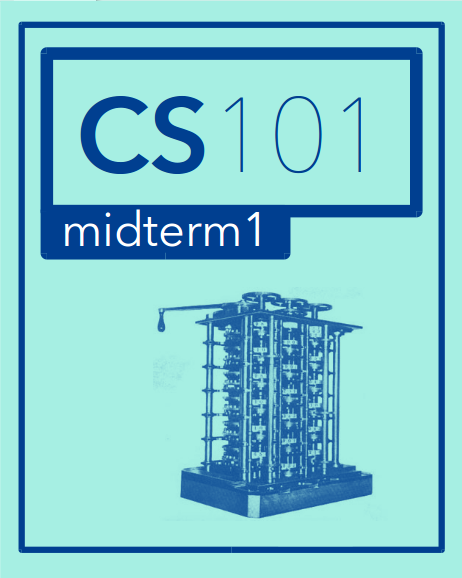
\includegraphics[width=2in]{../img/midterm1-header.png}
\end{center}

\bigskip
\noindent
\begin{itemize}
\item \textbf{Be sure to enter your \underline{NetID} and \underline{the code below} on your Scantron}.
\item Do not turn this page until instructed to do so.
\item There are 30 questions, worth 1 point each.
\item Each question has only \textbf{one} correct answer.
\item You must not communicate with other students during this test.
\item No books, notes, or electronic devices are permitted.
\item This is a 60-minute exam.
\item There are several different versions of this exam.
\end{itemize}

\bigskip\bigskip
\noindent
\textbf{\Large 1. Fill in your information:}

\bigskip
{\Large\bf
\begin{tabular}{ll}
Full Name: & \underbar{\hskip 8cm} \\[0.5em]
UIN (Student Number): & \underbar{\hskip 8cm} \\[0.5em]
NetID: & \underbar{\hskip 8cm}
\end{tabular}
}

\bigskip
\bigskip
\noindent
\textbf{\Large 2. Fill in the following answers on the Scantron form:}

%%%%%%%%%%%%%%%%%%%%%%%%%%%%%%%%%%%%%%%%%%%%%%%%%%%%%%%%%
%%%%%%%%%%%%%%%%%%%%%%%%%%%%%%%%%%%%%%%%%%%%%%%%%%%%%%%%%

\begin{enumerate}
\item[92.] D
\item[93.] B
\item[94.] A
\item[95.] C
\item[96.] C
\end{enumerate}

\newpage

% Zone 1


%%%%%%%%%%%%%%%%%%%%%%%%%%%%%%%%%%%%%%%%%%%%%%%%%%%%%%%%%



\newpage
\noindent
1. (1 point)
Consider the following program:
\begin{verbatim}
a=3
b=4
if a!=b:
    a=b
elif a==4:
    a=5
else:
    b=a
\end{verbatim}
What is the \textbf{value} of a after this program is executed?


\begin{enumerate}
\item[(A)]
None of the other answers are correct.

\item[(B)]
\begin{verbatim}3\end{verbatim}

\item[(C)] $\bigstar$ 
\begin{verbatim}4\end{verbatim}

\item[(D)]
\begin{verbatim}7\end{verbatim}

\item[(E)]
\begin{verbatim}5\end{verbatim}

\end{enumerate}

\vspace*{2em}
\hrule
\vspace{2em}

\noindent {\bf Solution.} 
\vspace{2em}
\hrule height 2pt


\newpage
\noindent
2. (1 point)
Consider the following program:
\begin{verbatim}
x=2
a=6
if (a%3)==2:
    x=x**3
elif(a%3)==1:
    x=x**2
else:
    x=x**1
\end{verbatim}
What is the \textbf{value} of \texttt{x} after this program is executed?


\begin{enumerate}
\item[(A)]
None of the other answers are correct.

\item[(B)]
\begin{verbatim}4\end{verbatim}

\item[(C)] $\bigstar$ 
\begin{verbatim}2\end{verbatim}

\item[(D)]
\begin{verbatim}8\end{verbatim}

\item[(E)]
\begin{verbatim}16\end{verbatim}

\end{enumerate}

\vspace*{2em}
\hrule
\vspace{2em}

\noindent {\bf Solution.} 
\vspace{2em}
\hrule height 2pt


\newpage
\noindent
3. (1 point)
Consider the following program.
\begin{verbatim}
x=[]
for j in range(0,5):
    if (j%2)==0:
        x.append("-")
    if (j%5)==0:
        x.append("*")
\end{verbatim}
After it is run, what is the final \textbf{value} of \texttt{x}?


\begin{enumerate}
\item[(A)]
\begin{verbatim}["-","*","-"]\end{verbatim}

\item[(B)]
\begin{verbatim}["-","-","*"]\end{verbatim}

\item[(C)]
\begin{verbatim}["*","-","*","*"]\end{verbatim}

\item[(D)] $\bigstar$ 
\begin{verbatim}["-","*","-","-"]\end{verbatim}

\item[(E)]
None of the other answers are correct.

\end{enumerate}

\vspace*{2em}
\hrule
\vspace{2em}

\noindent {\bf Solution.} 
\vspace{2em}
\hrule height 2pt


\newpage
\noindent
4. (1 point)
Evaluate the following expression:
\begin{verbatim}
[1,2]*len("3")
\end{verbatim}
What value is produced?


\begin{enumerate}
\item[(A)]
\begin{verbatim}[1,2,1]\end{verbatim}

\item[(B)]
\begin{verbatim}[1,2,1,2,1,2]\end{verbatim}

\item[(C)] $\bigstar$ 
\begin{verbatim}[1,2]\end{verbatim}

\item[(D)]
\begin{verbatim}[1,2,3]\end{verbatim}

\end{enumerate}

\vspace*{2em}
\hrule
\vspace{2em}

\noindent {\bf Solution.} 
\vspace{2em}
\hrule height 2pt


\newpage
\noindent
5. (1 point)
Consider the following incomplete program.
\begin{verbatim}
sum=0
for i in range(0,100):
    ???

\end{verbatim}
The program is intended to sum all of the integers between 1 and 100 (inclusive). What should replace the three question marks to complete the program?


\begin{enumerate}
\item[(A)]
\begin{verbatim}sum=sum+1\end{verbatim}

\item[(B)]
\begin{verbatim}sum+1=sum \end{verbatim}

\item[(C)]
\begin{verbatim}sum=sum+i \end{verbatim}

\item[(D)] $\bigstar$ 
\begin{verbatim}sum=sum+i+1 \end{verbatim}

\end{enumerate}

\vspace*{2em}
\hrule
\vspace{2em}

\noindent {\bf Solution.} 
\vspace{2em}
\hrule height 2pt


\newpage
\noindent
6. (1 point)
Consider the following program:
\begin{verbatim}
def fix(s):
    a=list(s)
    a.sort()
    return ''.join(a)

x=["one","two","eleven","twelve"]
s1=fix(x[0]+x[-1])
s2=fix(x[1]+x[-2])

if s1<s2:
    x.sort()
elif s1==s2:
    x.reverse()
else:
    x.append("six")
\end{verbatim}
What is the \textbf{value} of \texttt{x} after this program is executed?


\begin{enumerate}
\item[(A)]
\begin{verbatim}['one', 'two', 'eleven', 'twelve']\end{verbatim}

\item[(B)] $\bigstar$ 
\begin{verbatim}['twelve', 'eleven', 'two', 'one']\end{verbatim}

\item[(C)]
\begin{verbatim}['two', 'twelve', 'one', 'eleven', 'six']\end{verbatim}

\item[(D)]
\begin{verbatim}['one', 'two', 'eleven', 'twelve', 'six']\end{verbatim}

\item[(E)]
\begin{verbatim}['eleven', 'one', 'twelve', 'two']\end{verbatim}

\end{enumerate}

\vspace*{2em}
\hrule
\vspace{2em}

\noindent {\bf Solution.} 
\vspace{2em}
\hrule height 2pt


\newpage
\noindent
7. (1 point)
Consider the following incomplete function.
\begin{verbatim}
def isdivisible(m,n):
    if ???:
        return False
    else:
        return True
\end{verbatim}
The function is intended to return True if the input parameter m is evenly divisible by the parameter n and False otherwise. For example, \verb|isdivisible(4,2)| should return \verb|True|, but \verb|isdivisible(5,3)| should return \verb|False|. What should replace the three question marks to complete the function?


\begin{enumerate}
\item[(A)]
\begin{verbatim}(m // n) != 0 \end{verbatim}

\item[(B)]
\begin{verbatim}(n % m) == 0 \end{verbatim}

\item[(C)] $\bigstar$ 
\begin{verbatim}(m % n) != 0 \end{verbatim}

\item[(D)]
\begin{verbatim}(n // m) == 0 \end{verbatim}

\end{enumerate}

\vspace*{2em}
\hrule
\vspace{2em}

\noindent {\bf Solution.} 
\vspace{2em}
\hrule height 2pt


\newpage
\noindent
8. (1 point)
Consider the following program:
\begin{verbatim}
x=0
for i in range(4,10):
    if i%3==0:
        x+=3
    elif i%2==0:
        x+=2
    else:
        x+=1
\end{verbatim}
What is the \textbf{value} of \texttt{x} after this program is executed?


\begin{enumerate}
\item[(A)]
\begin{verbatim}10\end{verbatim}

\item[(B)] $\bigstar$ 
\begin{verbatim}12\end{verbatim}

\item[(C)]
\begin{verbatim}13\end{verbatim}

\item[(D)]
\begin{verbatim}11\end{verbatim}

\item[(E)]
\begin{verbatim}14\end{verbatim}

\end{enumerate}

\vspace*{2em}
\hrule
\vspace{2em}

\noindent {\bf Solution.} 
\vspace{2em}
\hrule height 2pt


\newpage
\noindent
9. (1 point)
Consider the following program.
\begin{verbatim}
def artificing(s):
    return s+"%i" % 2
    return s*2
    return s

s=artificing("MERLIN")
\end{verbatim}
After it is run, what is the final \textbf{value} of s?


\begin{enumerate}
\item[(A)]
\begin{verbatim}None\end{verbatim}

\item[(B)]
\begin{verbatim}"MERLIN%i"\end{verbatim}

\item[(C)]
\begin{verbatim}"MERLINMERLIN"\end{verbatim}

\item[(D)] $\bigstar$ 
\begin{verbatim}"MERLIN2"\end{verbatim}

\item[(E)]
\begin{verbatim}0\end{verbatim}

\end{enumerate}

\vspace*{2em}
\hrule
\vspace{2em}

\noindent {\bf Solution.} 
\vspace{2em}
\hrule height 2pt


\newpage
\noindent
10. (1 point)
How can the following mathematical equation be implemented as a Python expression? Assume \verb|a|, \verb|b|, and \verb|cos| have already been defined.
$$a^b \cos(a - b)$$


\begin{enumerate}
\item[(A)] $\bigstar$ 
\begin{verbatim}(a**b)*cos(a-b)\end{verbatim}

\item[(B)]
\begin{verbatim}(a**b)cos(a-b)\end{verbatim}

\item[(C)]
None of the other answers are correct.

\item[(D)]
\begin{verbatim}(a^b)*cos(a-b)\end{verbatim}

\item[(E)]
\begin{verbatim}(b^a)cos(a-b)\end{verbatim}

\end{enumerate}

\vspace*{2em}
\hrule
\vspace{2em}

\noindent {\bf Solution.} 
\vspace{2em}
\hrule height 2pt


\newpage
\noindent
11. (1 point)
Consider the following incomplete Python program.
\begin{verbatim}
s="".join(["2","2","0","1"])
x=0
for i in range(len(s)-1):
    x+=int(???)
\end{verbatim}
What should replace the three question marks so the resulting value of \texttt{x} is 43?


\begin{enumerate}
\item[(A)]
\begin{verbatim}s[i:i+1]\end{verbatim}

\item[(B)] $\bigstar$ 
\begin{verbatim}s[i:i+2]\end{verbatim}

\item[(C)]
\begin{verbatim}s[i:i-1]\end{verbatim}

\item[(D)]
\begin{verbatim}s[i+1:i+2]\end{verbatim}

\end{enumerate}

\vspace*{2em}
\hrule
\vspace{2em}

\noindent {\bf Solution.} 
\vspace{2em}
\hrule height 2pt


\newpage
\noindent
12. (1 point)
Consider the following program:
\begin{verbatim}
pi="3.14159"
e="2.71828"
x=(float(e)**float(pi)-float(pi)) == 20
\end{verbatim}
What is the \textbf{type} of \texttt{x} after this program is executed?


\begin{enumerate}
\item[(A)] $\bigstar$ 
\begin{verbatim}Boolean\end{verbatim}

\item[(B)]
\begin{verbatim}String\end{verbatim}

\item[(C)]
\begin{verbatim}Float\end{verbatim}

\item[(D)]
\begin{verbatim}Integer\end{verbatim}

\item[(E)]
\begin{verbatim}None\end{verbatim}

\end{enumerate}

\vspace*{2em}
\hrule
\vspace{2em}

\noindent {\bf Solution.} 
\vspace{2em}
\hrule height 2pt


\newpage
\noindent
13. (1 point)
What is the result of the following expression?
\begin{verbatim}
[ 1, 2, 3 ] * 3.0
\end{verbatim}


\begin{enumerate}
\item[(A)]
\begin{verbatim}[3, 6, 9]\end{verbatim}

\item[(B)] $\bigstar$ 
\begin{verbatim}[1, 2, 3, 1, 2, 3, 1, 2, 3]\end{verbatim}

\item[(C)]
\begin{verbatim}[1.0, 2.0, 3.0, 1.0, 2.0, 3.0, 1.0, 2.0, 3.0]\end{verbatim}

\item[(D)]
\begin{verbatim}[3.0, 6.0, 9.0]\end{verbatim}

\item[(E)]
\begin{verbatim}None of the above.\end{verbatim}

\end{enumerate}

\vspace*{2em}
\hrule
\vspace{2em}

\noindent {\bf Solution.} 
\vspace{2em}
\hrule height 2pt


\newpage
\noindent
14. (1 point)
Consider the following Python program.
\begin{verbatim}
e=[1,3,5,7,9,11]
d=[0,0,0]
for i in range(0,len(e)):
    d[i%3]+=e[i]
x=d[2]
\end{verbatim}
After it is run, what is the final \textbf{value} of \texttt{x}?


\begin{enumerate}
\item[(A)] $\bigstar$ 
\begin{verbatim}16\end{verbatim}

\item[(B)]
\begin{verbatim}7\end{verbatim}

\item[(C)]
\begin{verbatim}12\end{verbatim}

\item[(D)]
\begin{verbatim}0\end{verbatim}

\item[(E)]
\begin{verbatim}8\end{verbatim}

\end{enumerate}

\vspace*{2em}
\hrule
\vspace{2em}

\noindent {\bf Solution.} 
\vspace{2em}
\hrule height 2pt


\newpage
\noindent
15. (1 point)
For this problem, you should compose a function which accomplishes a given task using the available code blocks arranged in the correct functional order.  \emph{We ignore indentation for this problem.}

\texttt{find\_max} should accept a \texttt{list} and return the value of the maximum item in the \texttt{list}.  (\texttt{None} is always the lowest value in any numeric comparison, so you may use it as an initializer.)

\begin{verbatim}
def find_max(my_list):
\end{verbatim}

\begin{enumerate}[1]
\item \texttt{max\_val = i}
\item \texttt{max\_val = None}
\item \texttt{for i in range(len(my\_list)):}
\item \texttt{if i > max\_val:}
\item \texttt{max\_val = my\_list[i]}
\item \texttt{return max\_val}
\item \texttt{for i in range(my\_list):}
\item \texttt{if my\_list[i] > max\_val:}
\item \texttt{print(max\_val)}
\end{enumerate}



\begin{enumerate}
\item[(A)]
2, 7, 4, 5, 6

\item[(B)]
2, 3, 8, 1, 6

\item[(C)] $\bigstar$ 
2, 3, 8, 5, 6

\item[(D)]
3, 2, 8, 5, 9

\item[(E)]
2, 3, 4, 1, 6

\end{enumerate}

\vspace*{2em}
\hrule
\vspace{2em}

\noindent {\bf Solution.} 
\vspace{2em}
\hrule height 2pt


\newpage
\noindent
16. (1 point)
Consider the following program:
\begin{verbatim}
x=[1,2,3]
def f(a):
    s=""
    a.append(4)
    for i in a:
        s+=str(i)
    return s

x.append(f(x))
\end{verbatim}
What is the \textbf{value} of \texttt{x} after this program is executed?


\begin{enumerate}
\item[(A)]
\begin{verbatim}[1, 2, 3, '1234']\end{verbatim}

\item[(B)]
\begin{verbatim}[1, 2, 3, '123']\end{verbatim}

\item[(C)] $\bigstar$ 
\begin{verbatim}[1, 2, 3, 4, '1234']\end{verbatim}

\item[(D)]
\begin{verbatim}[1, 2, 3, 10]\end{verbatim}

\item[(E)]
\begin{verbatim}[1, 2, 3]\end{verbatim}

\end{enumerate}

\vspace*{2em}
\hrule
\vspace{2em}

\noindent {\bf Solution.} 
\vspace{2em}
\hrule height 2pt


\newpage
\noindent
17. (1 point)
Consider the following program:
\begin{verbatim}
i=3
x=2
while i < 7:
    x+=i
    i+=2
\end{verbatim}
What is the \textbf{value} of \texttt{x} after this program is executed?


\begin{enumerate}
\item[(A)]
\begin{verbatim}14\end{verbatim}

\item[(B)]
\begin{verbatim}13\end{verbatim}

\item[(C)]
\begin{verbatim}12\end{verbatim}

\item[(D)] $\bigstar$ 
\begin{verbatim}10\end{verbatim}

\item[(E)]
\begin{verbatim}11\end{verbatim}

\end{enumerate}

\vspace*{2em}
\hrule
\vspace{2em}

\noindent {\bf Solution.} 
\vspace{2em}
\hrule height 2pt


\newpage
\noindent
18. (1 point)
Consider the following program.
\begin{verbatim}
s="ABCBA"
x=0
y=len(s)-1
while s[x]==s[y] and x<=y:
    x+=1
    y-=1
\end{verbatim}
After it is run, what is the final \textbf{value} of \texttt{x}?


\begin{enumerate}
\item[(A)]
\begin{verbatim}0\end{verbatim}

\item[(B)]
\begin{verbatim}1\end{verbatim}

\item[(C)] $\bigstar$ 
\begin{verbatim}3\end{verbatim}

\item[(D)]
\begin{verbatim}4\end{verbatim}

\item[(E)]
\begin{verbatim}2\end{verbatim}

\end{enumerate}

\vspace*{2em}
\hrule
\vspace{2em}

\noindent {\bf Solution.} 
\vspace{2em}
\hrule height 2pt


\newpage
\noindent
19. (1 point)
Consider the following program:
\begin{verbatim}
a=["merlin","sir agravaine","king pellinore"]
b=[ ]
for i in range(0,4):
    b.append(a[0-i].title())
\end{verbatim}
What is the \textbf{value} of b after this program is executed?


\begin{enumerate}
\item[(A)]
\begin{verbatim}['King Pellinore', 'Sir Agravaine', 'Merlin']\end{verbatim}

\item[(B)]
\begin{verbatim}[ ]\end{verbatim}

\item[(C)]
\begin{verbatim}['Merlin', 'King Pellinore', 'Sir Agravaine']\end{verbatim}

\item[(D)]
\begin{verbatim}['Merlin', 'Sir Agravaine', 'King Pellinore', 'Merlin']\end{verbatim}

\item[(E)] $\bigstar$ 
\begin{verbatim}['Merlin', 'King Pellinore', 'Sir Agravaine', 'Merlin']\end{verbatim}

\end{enumerate}

\vspace*{2em}
\hrule
\vspace{2em}

\noindent {\bf Solution.} 
\vspace{2em}
\hrule height 2pt


\newpage
\noindent
20. (1 point)
Consider the following program:
\begin{verbatim}
s="-B-O-R-S-"
x=s.split("-")[2:-2]
\end{verbatim}
What is the \textbf{value} of \texttt{x} after this program is executed?


\begin{enumerate}
\item[(A)]
\begin{verbatim}None\end{verbatim}

\item[(B)] $\bigstar$ 
\begin{verbatim}['O', 'R']\end{verbatim}

\item[(C)]
\begin{verbatim}'ORS'\end{verbatim}

\item[(D)]
\begin{verbatim}''\end{verbatim}

\item[(E)]
\begin{verbatim}False\end{verbatim}

\end{enumerate}

\vspace*{2em}
\hrule
\vspace{2em}

\noindent {\bf Solution.} 
\vspace{2em}
\hrule height 2pt


\newpage
\noindent
21. (1 point)
Consider the following program.
\begin{verbatim}
kay = 2
wart = 3

def knight(kay,wart):
    wart += 2
    kay += 3
    return wart + kay

wart = knight(kay, kay) + knight(wart, wart)
\end{verbatim}
After it is run, what is the final \textbf{value} of \texttt{wart}?


\begin{enumerate}
\item[(A)]
\begin{verbatim}2\end{verbatim}

\item[(B)] $\bigstar$ 
None of the other answers are correct.

\item[(C)]
\begin{verbatim}3\end{verbatim}

\item[(D)]
\begin{verbatim}5\end{verbatim}

\end{enumerate}

\vspace*{2em}
\hrule
\vspace{2em}

\noindent {\bf Solution.} 
\vspace{2em}
\hrule height 2pt


\newpage
\noindent
22. (1 point)
Consider the following program:
\begin{verbatim}
x=[1,2,3,4,5,6,7,8,9]
x=x[2:-2]
i=1
while i <= 3:
    x[i]+=1
    i+=1
\end{verbatim}
What is the \textbf{value} of \texttt{x} after this program is executed?


\begin{enumerate}
\item[(A)]
\begin{verbatim}[2, 4, 5, 5, 7, 7]\end{verbatim}

\item[(B)] $\bigstar$ 
\begin{verbatim}[3, 5, 6, 7, 7]\end{verbatim}

\item[(C)]
\begin{verbatim}[3, 5, 7, 7]\end{verbatim}

\item[(D)]
\begin{verbatim}[3, 5, 6, 7, 7, 8]\end{verbatim}

\item[(E)]
\begin{verbatim}[2, 4, 5, 6, 7, 7]\end{verbatim}

\end{enumerate}

\vspace*{2em}
\hrule
\vspace{2em}

\noindent {\bf Solution.} 
\vspace{2em}
\hrule height 2pt


\newpage
\noindent
23. (1 point)
Consider the following program:
\begin{verbatim}
x=str(1.2)*2
\end{verbatim}
What is the \textbf{value} of \texttt{x} after this program is executed?


\begin{enumerate}
\item[(A)]
\begin{verbatim}"2.4"\end{verbatim}

\item[(B)] $\bigstar$ 
\begin{verbatim}"1.21.2"\end{verbatim}

\item[(C)]
\begin{verbatim}2.4\end{verbatim}

\item[(D)]
None of the other answers are correct.

\item[(E)]
\begin{verbatim}"1.2*2"\end{verbatim}

\end{enumerate}

\vspace*{2em}
\hrule
\vspace{2em}

\noindent {\bf Solution.} 
\vspace{2em}
\hrule height 2pt


\newpage
\noindent
24. (1 point)
Consider the following program.
\begin{verbatim}
x=0
i=1
while(i*i)<=9:
    x=x+(i*i)
    i=i+1
\end{verbatim}
After it is run, what is the final \textbf{value} of \texttt{x}?


\begin{enumerate}
\item[(A)]
\begin{verbatim}3\end{verbatim}

\item[(B)]
\begin{verbatim}30\end{verbatim}

\item[(C)]
\begin{verbatim}5\end{verbatim}

\item[(D)] $\bigstar$ 
\begin{verbatim}14\end{verbatim}

\item[(E)]
\begin{verbatim}4\end{verbatim}

\end{enumerate}

\vspace*{2em}
\hrule
\vspace{2em}

\noindent {\bf Solution.} 
\vspace{2em}
\hrule height 2pt


\newpage
\noindent
25. (1 point)
Evaluate the following expression:
\begin{verbatim}
len("ABCD"[0:3])
\end{verbatim}
What value is produced?


\begin{enumerate}
\item[(A)] $\bigstar$ 
3

\item[(B)]
4

\item[(C)]
2

\item[(D)]
1

\end{enumerate}

\vspace*{2em}
\hrule
\vspace{2em}

\noindent {\bf Solution.} 
\vspace{2em}
\hrule height 2pt


\newpage
\noindent
26. (1 point)
Consider the following program:
\begin{verbatim}
s="Hobbes"
i=0
x=-1
while i<len(s):
    if s[i]=='b':
        x=i
    i+=1
\end{verbatim}
What is the \textbf{value} of \texttt{x} after this program is executed?


\begin{enumerate}
\item[(A)]
\begin{verbatim}5\end{verbatim}

\item[(B)]
\begin{verbatim}2\end{verbatim}

\item[(C)] $\bigstar$ 
\begin{verbatim}3\end{verbatim}

\item[(D)]
\begin{verbatim}4\end{verbatim}

\item[(E)]
\begin{verbatim}-1\end{verbatim}

\end{enumerate}

\vspace*{2em}
\hrule
\vspace{2em}

\noindent {\bf Solution.} 
\vspace{2em}
\hrule height 2pt


\newpage
\noindent
27. (1 point)
Consider the following program:
\begin{verbatim}
s="ECTOR"
t="GAWAIN"
x=(len(s)/(len(t)-1))+1
\end{verbatim}
What is the \textbf{type} of \texttt{x} after this program is executed?


\begin{enumerate}
\item[(A)]
\begin{verbatim}Boolean\end{verbatim}

\item[(B)] $\bigstar$ 
\begin{verbatim}Float\end{verbatim}

\item[(C)]
\begin{verbatim}Integer\end{verbatim}

\item[(D)]
\begin{verbatim}None\end{verbatim}

\item[(E)]
\begin{verbatim}String\end{verbatim}

\end{enumerate}

\vspace*{2em}
\hrule
\vspace{2em}

\noindent {\bf Solution.} 
\vspace{2em}
\hrule height 2pt


\newpage
\noindent
28. (1 point)
Consider the following program:
\begin{verbatim}
a=["S","T","U","P","E","F","Y"]
a=a[0:4]
a.sort()
x=""
for e in a:
    x=e+x
\end{verbatim}
What is the \textbf{value} of \texttt{x} after this program is executed?


\begin{enumerate}
\item[(A)]
\begin{verbatim}"STUP"\end{verbatim}

\item[(B)]
\begin{verbatim}"PSTU"\end{verbatim}

\item[(C)]
\begin{verbatim}"PUST"\end{verbatim}

\item[(D)] $\bigstar$ 
\begin{verbatim}"UTSP"\end{verbatim}

\item[(E)]
None of the other answers are correct.

\end{enumerate}

\vspace*{2em}
\hrule
\vspace{2em}

\noindent {\bf Solution.} 
\vspace{2em}
\hrule height 2pt


\newpage
\noindent
29. (1 point)
Consider the following program:
\begin{verbatim}
x="KING ARTHUR-MORGANA LEFAY-SIR BEDIVERE".split("-")
y=x[:]
y.reverse()
\end{verbatim}
What is the \textbf{value} of \texttt{x} after this program is executed?


\begin{enumerate}
\item[(A)]
\begin{verbatim}['SIR BEDIVERE', 'MORGANA LEFAY', 'KING ARTHUR']\end{verbatim}

\item[(B)]
\begin{verbatim}['BEDIVERE', 'LEFAY-SIR', 'ARTHUR-MORGANA', 'KING']\end{verbatim}

\item[(C)]
\begin{verbatim}['KING', 'ARTHUR-MORGANA', 'LEFAY-SIR', 'BEDIVERE']\end{verbatim}

\item[(D)] $\bigstar$ 
\begin{verbatim}['KING ARTHUR', 'MORGANA LEFAY', 'SIR BEDIVERE']\end{verbatim}

\item[(E)]
\begin{verbatim}None\end{verbatim}

\end{enumerate}

\vspace*{2em}
\hrule
\vspace{2em}

\noindent {\bf Solution.} 
\vspace{2em}
\hrule height 2pt


\newpage
\noindent
30. (1 point)
Consider the following program:
\begin{verbatim}
s="TRIS %i"
t="ISEU"
x=len(s) % len(t[2:-1])
\end{verbatim}
What is the \textbf{type} of \texttt{x} after this program is executed?


\begin{enumerate}
\item[(A)]
\begin{verbatim}Boolean\end{verbatim}

\item[(B)]
\begin{verbatim}String\end{verbatim}

\item[(C)]
\begin{verbatim}Float\end{verbatim}

\item[(D)]
\begin{verbatim}None\end{verbatim}

\item[(E)] $\bigstar$ 
\begin{verbatim}Integer\end{verbatim}

\end{enumerate}

\vspace*{2em}
\hrule
\vspace{2em}

\noindent {\bf Solution.} 
\vspace{2em}
\hrule height 2pt

%%%%%%%%%%%%%%%%%%%%%%%%%%%%%%%%%%%%%%%%%%%%%%%%%%%%%%%%%%%%%%%%%%%%%%
%%%%%%%%%%%%%%%%%%%%%%%%%%%%%%%%%%%%%%%%%%%%%%%%%%%%%%%%%%%%%%%%%%%%%%
%%%%%%%%%%%%%%%%%%%%%%%%%%%%%%%%%%%%%%%%%%%%%%%%%%%%%%%%%%%%%%%%%%%%%%
%%%%%%%%%%%%%%%%%%%%%%%%%%%%%%%%%%%%%%%%%%%%%%%%%%%%%%%%%%%%%%%%%%%%%%
% Exam number 10

\message{Exam 10/50}
\cleardoublepage
\setcounter{page}{1}


\begin{center}
%\textbf{\Large CS 101 Midterm \#1}
%
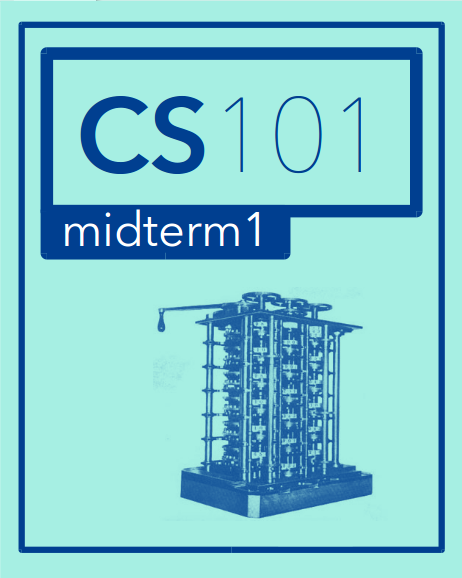
\includegraphics[width=2in]{../img/midterm1-header.png}
\end{center}

\bigskip
\noindent
\begin{itemize}
\item \textbf{Be sure to enter your \underline{NetID} and \underline{the code below} on your Scantron}.
\item Do not turn this page until instructed to do so.
\item There are 30 questions, worth 1 point each.
\item Each question has only \textbf{one} correct answer.
\item You must not communicate with other students during this test.
\item No books, notes, or electronic devices are permitted.
\item This is a 60-minute exam.
\item There are several different versions of this exam.
\end{itemize}

\bigskip\bigskip
\noindent
\textbf{\Large 1. Fill in your information:}

\bigskip
{\Large\bf
\begin{tabular}{ll}
Full Name: & \underbar{\hskip 8cm} \\[0.5em]
UIN (Student Number): & \underbar{\hskip 8cm} \\[0.5em]
NetID: & \underbar{\hskip 8cm}
\end{tabular}
}

\bigskip
\bigskip
\noindent
\textbf{\Large 2. Fill in the following answers on the Scantron form:}

%%%%%%%%%%%%%%%%%%%%%%%%%%%%%%%%%%%%%%%%%%%%%%%%%%%%%%%%%
%%%%%%%%%%%%%%%%%%%%%%%%%%%%%%%%%%%%%%%%%%%%%%%%%%%%%%%%%

\begin{enumerate}
\item[92.] E
\item[93.] B
\item[94.] A
\item[95.] D
\item[96.] D
\end{enumerate}

\newpage

% Zone 1


%%%%%%%%%%%%%%%%%%%%%%%%%%%%%%%%%%%%%%%%%%%%%%%%%%%%%%%%%



\newpage
\noindent
1. (1 point)
Consider the following program:
\begin{verbatim}
x="KING ARTHUR-MORGANA LEFAY-SIR BEDIVERE".split("-")
y=x
x=y.reverse()
\end{verbatim}
What is the \textbf{value} of \texttt{x} after this program is executed?


\begin{enumerate}
\item[(A)] $\bigstar$ 
\begin{verbatim}None\end{verbatim}

\item[(B)]
\begin{verbatim}['KING ARTHUR', 'MORGANA LEFAY', 'SIR BEDIVERE']\end{verbatim}

\item[(C)]
\begin{verbatim}['KING', 'ARTHUR-MORGANA', 'LEFAY-SIR', 'BEDIVERE']\end{verbatim}

\item[(D)]
\begin{verbatim}['SIR BEDIVERE', 'MORGANA LEFAY', 'KING ARTHUR']\end{verbatim}

\item[(E)]
\begin{verbatim}['BEDIVERE', 'LEFAY-SIR', 'ARTHUR-MORGANA', 'KING']\end{verbatim}

\end{enumerate}

\vspace*{2em}
\hrule
\vspace{2em}

\noindent {\bf Solution.} 
\vspace{2em}
\hrule height 2pt


\newpage
\noindent
2. (1 point)
Consider the following program:
\begin{verbatim}
s="-B-O-R-S-"
x=s.split("-")[2:-2]
\end{verbatim}
What is the \textbf{value} of \texttt{x} after this program is executed?


\begin{enumerate}
\item[(A)]
\begin{verbatim}None\end{verbatim}

\item[(B)]
\begin{verbatim}'ORS'\end{verbatim}

\item[(C)] $\bigstar$ 
\begin{verbatim}['O', 'R']\end{verbatim}

\item[(D)]
\begin{verbatim}''\end{verbatim}

\item[(E)]
\begin{verbatim}False\end{verbatim}

\end{enumerate}

\vspace*{2em}
\hrule
\vspace{2em}

\noindent {\bf Solution.} 
\vspace{2em}
\hrule height 2pt


\newpage
\noindent
3. (1 point)
Consider the following program:
\begin{verbatim}
i=3
x=2
while i < 7:
    x+=i
    i+=2
\end{verbatim}
What is the \textbf{value} of \texttt{x} after this program is executed?


\begin{enumerate}
\item[(A)]
\begin{verbatim}14\end{verbatim}

\item[(B)] $\bigstar$ 
\begin{verbatim}10\end{verbatim}

\item[(C)]
\begin{verbatim}13\end{verbatim}

\item[(D)]
\begin{verbatim}11\end{verbatim}

\item[(E)]
\begin{verbatim}12\end{verbatim}

\end{enumerate}

\vspace*{2em}
\hrule
\vspace{2em}

\noindent {\bf Solution.} 
\vspace{2em}
\hrule height 2pt


\newpage
\noindent
4. (1 point)
What is the result of the following expression?
\begin{verbatim}
[ 1, 2, 3 ] * 3.0
\end{verbatim}


\begin{enumerate}
\item[(A)] $\bigstar$ 
\begin{verbatim}[1, 2, 3, 1, 2, 3, 1, 2, 3]\end{verbatim}

\item[(B)]
\begin{verbatim}[1.0, 2.0, 3.0, 1.0, 2.0, 3.0, 1.0, 2.0, 3.0]\end{verbatim}

\item[(C)]
\begin{verbatim}[3.0, 6.0, 9.0]\end{verbatim}

\item[(D)]
\begin{verbatim}None of the above.\end{verbatim}

\item[(E)]
\begin{verbatim}[3, 6, 9]\end{verbatim}

\end{enumerate}

\vspace*{2em}
\hrule
\vspace{2em}

\noindent {\bf Solution.} 
\vspace{2em}
\hrule height 2pt


\newpage
\noindent
5. (1 point)
Consider the following program:
\begin{verbatim}
pi="3.14159"
e="2.71828"
x=pi*len(e)+pi
\end{verbatim}
What is the \textbf{type} of \texttt{x} after this program is executed?


\begin{enumerate}
\item[(A)]
\begin{verbatim}Integer\end{verbatim}

\item[(B)]
\begin{verbatim}None\end{verbatim}

\item[(C)] $\bigstar$ 
\begin{verbatim}String\end{verbatim}

\item[(D)]
\begin{verbatim}Float\end{verbatim}

\item[(E)]
\begin{verbatim}Boolean\end{verbatim}

\end{enumerate}

\vspace*{2em}
\hrule
\vspace{2em}

\noindent {\bf Solution.} 
\vspace{2em}
\hrule height 2pt


\newpage
\noindent
6. (1 point)
Evaluate the following expression:
\begin{verbatim}
len("ABCDE"[1:4])
\end{verbatim}
What value is produced?


\begin{enumerate}
\item[(A)]
1

\item[(B)]
4

\item[(C)] $\bigstar$ 
3

\item[(D)]
5

\end{enumerate}

\vspace*{2em}
\hrule
\vspace{2em}

\noindent {\bf Solution.} 
\vspace{2em}
\hrule height 2pt


\newpage
\noindent
7. (1 point)
Consider the following program:
\begin{verbatim}
s="TRIS %i"
t="ISEU"
x=s % len(t)
\end{verbatim}
What is the \textbf{type} of \texttt{x} after this program is executed?


\begin{enumerate}
\item[(A)]
\begin{verbatim}Integer\end{verbatim}

\item[(B)]
\begin{verbatim}None\end{verbatim}

\item[(C)]
\begin{verbatim}Float\end{verbatim}

\item[(D)]
\begin{verbatim}Boolean\end{verbatim}

\item[(E)] $\bigstar$ 
\begin{verbatim}String\end{verbatim}

\end{enumerate}

\vspace*{2em}
\hrule
\vspace{2em}

\noindent {\bf Solution.} 
\vspace{2em}
\hrule height 2pt


\newpage
\noindent
8. (1 point)
Consider the following program:
\begin{verbatim}
x=[1,2,3]
def f(a):
    s=""
    a.reverse()
    for i in a:
        s+=str(i)
    return s

x.append(f(x))
\end{verbatim}
What is the \textbf{value} of \texttt{x} after this program is executed?


\begin{enumerate}
\item[(A)]
\begin{verbatim}[1, 2, 3, 6]\end{verbatim}

\item[(B)]
\begin{verbatim}[3, 2, 1]\end{verbatim}

\item[(C)] $\bigstar$ 
\begin{verbatim}[3, 2, 1, '321']\end{verbatim}

\item[(D)]
\begin{verbatim}[1, 2, 3, '321']\end{verbatim}

\item[(E)]
\begin{verbatim}[1, 2, 3]\end{verbatim}

\end{enumerate}

\vspace*{2em}
\hrule
\vspace{2em}

\noindent {\bf Solution.} 
\vspace{2em}
\hrule height 2pt


\newpage
\noindent
9. (1 point)
Consider the following program:
\begin{verbatim}
def fix(s):
    a=list(s)
    a.sort()
    return ''.join(a)

x=["one","two","eleven","twelve"]
s1=fix(x[0]+x[-1])
s2=fix(x[1]+x[-2])

if s1<s2:
    x.sort()
elif s1>s2:
    x.reverse()
else:
    x.append("six")
\end{verbatim}
What is the \textbf{value} of \texttt{x} after this program is executed?


\begin{enumerate}
\item[(A)]
\begin{verbatim}['eleven', 'one', 'twelve', 'two']\end{verbatim}

\item[(B)] $\bigstar$ 
\begin{verbatim}['one', 'two', 'eleven', 'twelve', 'six']\end{verbatim}

\item[(C)]
\begin{verbatim}['twelve', 'eleven', 'two', 'one']\end{verbatim}

\item[(D)]
\begin{verbatim}['two', 'twelve', 'one', 'eleven', 'six']\end{verbatim}

\item[(E)]
\begin{verbatim}['one', 'two', 'eleven', 'twelve']\end{verbatim}

\end{enumerate}

\vspace*{2em}
\hrule
\vspace{2em}

\noindent {\bf Solution.} 
\vspace{2em}
\hrule height 2pt


\newpage
\noindent
10. (1 point)
Consider the following program.
\begin{verbatim}
x=0
i=1
while(i*i)<=9:
    x=x+(i*i)
    i=i+1
\end{verbatim}
After it is run, what is the final \textbf{value} of \texttt{x}?


\begin{enumerate}
\item[(A)]
\begin{verbatim}5\end{verbatim}

\item[(B)] $\bigstar$ 
\begin{verbatim}14\end{verbatim}

\item[(C)]
\begin{verbatim}4\end{verbatim}

\item[(D)]
\begin{verbatim}30\end{verbatim}

\item[(E)]
\begin{verbatim}3\end{verbatim}

\end{enumerate}

\vspace*{2em}
\hrule
\vspace{2em}

\noindent {\bf Solution.} 
\vspace{2em}
\hrule height 2pt


\newpage
\noindent
11. (1 point)
Consider the following Python program.
\begin{verbatim}
e=[1,3,5,7,9,11]
d=[0,0,0]
for i in range(0,len(e)):
    d[i%3]+=e[i]
x=d[1]
\end{verbatim}
After it is run, what is the final \textbf{value} of \texttt{x}?


\begin{enumerate}
\item[(A)] $\bigstar$ 
\begin{verbatim}12\end{verbatim}

\item[(B)]
\begin{verbatim}0\end{verbatim}

\item[(C)]
\begin{verbatim}8\end{verbatim}

\item[(D)]
\begin{verbatim}3\end{verbatim}

\item[(E)]
\begin{verbatim}16\end{verbatim}

\end{enumerate}

\vspace*{2em}
\hrule
\vspace{2em}

\noindent {\bf Solution.} 
\vspace{2em}
\hrule height 2pt


\newpage
\noindent
12. (1 point)
Consider the following program.
\begin{verbatim}
kay = 2
wart = 3

def knight(kay,wart):
    wart += 2
    kay += 3
    return wart + kay

wart = knight(kay, kay) + knight(wart, wart)
\end{verbatim}
After it is run, what is the final \textbf{value} of \texttt{wart}?


\begin{enumerate}
\item[(A)] $\bigstar$ 
None of the other answers are correct.

\item[(B)]
\begin{verbatim}2\end{verbatim}

\item[(C)]
\begin{verbatim}5\end{verbatim}

\item[(D)]
\begin{verbatim}3\end{verbatim}

\end{enumerate}

\vspace*{2em}
\hrule
\vspace{2em}

\noindent {\bf Solution.} 
\vspace{2em}
\hrule height 2pt


\newpage
\noindent
13. (1 point)
Consider the following program:
\begin{verbatim}
x=0
for i in range(2,8):
    if i%3==0:
        x+=3
    elif i%2==0:
        x+=2
    else:
        x+=1
\end{verbatim}
What is the \textbf{value} of \texttt{x} after this program is executed?


\begin{enumerate}
\item[(A)]
\begin{verbatim}14\end{verbatim}

\item[(B)]
\begin{verbatim}10\end{verbatim}

\item[(C)] $\bigstar$ 
\begin{verbatim}12\end{verbatim}

\item[(D)]
\begin{verbatim}13\end{verbatim}

\item[(E)]
\begin{verbatim}11\end{verbatim}

\end{enumerate}

\vspace*{2em}
\hrule
\vspace{2em}

\noindent {\bf Solution.} 
\vspace{2em}
\hrule height 2pt


\newpage
\noindent
14. (1 point)
Consider the following program:
\begin{verbatim}
x=3
a=7
if (a%3)==2:
    x=x**2
elif(a%3)==1:
    x=x**1
else:
    x=x**0
\end{verbatim}
What is the \textbf{value} of \texttt{x} after this program is executed?


\begin{enumerate}
\item[(A)]
\begin{verbatim}7\end{verbatim}

\item[(B)] $\bigstar$ 
\begin{verbatim}3\end{verbatim}

\item[(C)]
\begin{verbatim}1\end{verbatim}

\item[(D)]
\begin{verbatim}9\end{verbatim}

\item[(E)]
None of the other answers are correct.

\end{enumerate}

\vspace*{2em}
\hrule
\vspace{2em}

\noindent {\bf Solution.} 
\vspace{2em}
\hrule height 2pt


\newpage
\noindent
15. (1 point)
Consider the following program:
\begin{verbatim}
s="Calvin"
i=0
x=-1
while i<len(s):
    if s[i]=='b':
        x=i
    i+=1
\end{verbatim}
What is the \textbf{value} of \texttt{x} after this program is executed?


\begin{enumerate}
\item[(A)]
\begin{verbatim}5\end{verbatim}

\item[(B)]
\begin{verbatim}6\end{verbatim}

\item[(C)]
\begin{verbatim}3\end{verbatim}

\item[(D)] $\bigstar$ 
\begin{verbatim}-1\end{verbatim}

\item[(E)]
\begin{verbatim}0\end{verbatim}

\end{enumerate}

\vspace*{2em}
\hrule
\vspace{2em}

\noindent {\bf Solution.} 
\vspace{2em}
\hrule height 2pt


\newpage
\noindent
16. (1 point)
How can the following mathematical equation be implemented as a Python expression? Assume \verb|a|, \verb|b|, and \verb|cos| have already been defined.
$$a^b \cos(a - b)$$


\begin{enumerate}
\item[(A)]
\begin{verbatim}(b^a)cos(a-b)\end{verbatim}

\item[(B)]
\begin{verbatim}(a**b)cos(a-b)\end{verbatim}

\item[(C)] $\bigstar$ 
\begin{verbatim}(a**b)*cos(a-b)\end{verbatim}

\item[(D)]
\begin{verbatim}(a^b)*cos(a-b)\end{verbatim}

\item[(E)]
None of the other answers are correct.

\end{enumerate}

\vspace*{2em}
\hrule
\vspace{2em}

\noindent {\bf Solution.} 
\vspace{2em}
\hrule height 2pt


\newpage
\noindent
17. (1 point)
Consider the following program.
\begin{verbatim}
def artificing(s):
    return s+"%i" % 2
    return s*2
    return s

s=artificing("MERLIN")
\end{verbatim}
After it is run, what is the final \textbf{value} of s?


\begin{enumerate}
\item[(A)]
\begin{verbatim}0\end{verbatim}

\item[(B)]
\begin{verbatim}"MERLINMERLIN"\end{verbatim}

\item[(C)]
\begin{verbatim}"MERLIN%i"\end{verbatim}

\item[(D)]
\begin{verbatim}None\end{verbatim}

\item[(E)] $\bigstar$ 
\begin{verbatim}"MERLIN2"\end{verbatim}

\end{enumerate}

\vspace*{2em}
\hrule
\vspace{2em}

\noindent {\bf Solution.} 
\vspace{2em}
\hrule height 2pt


\newpage
\noindent
18. (1 point)
Consider the following program:
\begin{verbatim}
s="ECTOR"
t="GAWAIN"
x=len(str(s.isupper()))-t.find("A")
\end{verbatim}
What is the \textbf{type} of \texttt{x} after this program is executed?


\begin{enumerate}
\item[(A)] $\bigstar$ 
\begin{verbatim}Integer\end{verbatim}

\item[(B)]
\begin{verbatim}Float\end{verbatim}

\item[(C)]
\begin{verbatim}Boolean\end{verbatim}

\item[(D)]
\begin{verbatim}String\end{verbatim}

\item[(E)]
\begin{verbatim}None\end{verbatim}

\end{enumerate}

\vspace*{2em}
\hrule
\vspace{2em}

\noindent {\bf Solution.} 
\vspace{2em}
\hrule height 2pt


\newpage
\noindent
19. (1 point)
For this problem, you should compose a function which accomplishes a given task using the available code blocks arranged in the correct functional order.  \emph{We ignore indentation for this problem.}

\texttt{find\_max} should accept a \texttt{list} and return the value of the maximum item in the \texttt{list}.  (\texttt{None} is always the lowest value in any numeric comparison, so you may use it as an initializer.)

\begin{verbatim}
def find_max(my_list):
\end{verbatim}

\begin{enumerate}[1]
\item \texttt{max\_val = i}
\item \texttt{max\_val = None}
\item \texttt{for i in range(len(my\_list)):}
\item \texttt{if i > max\_val:}
\item \texttt{max\_val = my\_list[i]}
\item \texttt{return max\_val}
\item \texttt{for i in range(my\_list):}
\item \texttt{if my\_list[i] > max\_val:}
\item \texttt{print(max\_val)}
\end{enumerate}



\begin{enumerate}
\item[(A)]
2, 7, 4, 5, 6

\item[(B)]
3, 2, 8, 5, 9

\item[(C)] $\bigstar$ 
2, 3, 8, 5, 6

\item[(D)]
2, 3, 8, 1, 6

\item[(E)]
2, 3, 4, 1, 6

\end{enumerate}

\vspace*{2em}
\hrule
\vspace{2em}

\noindent {\bf Solution.} 
\vspace{2em}
\hrule height 2pt


\newpage
\noindent
20. (1 point)
Consider the following program:
\begin{verbatim}
a=["S","T","U","P","E","F","Y"]
a=a[0:4]
a.sort()
x=""
for e in a:
    x=e+x
\end{verbatim}
What is the \textbf{value} of \texttt{x} after this program is executed?


\begin{enumerate}
\item[(A)]
\begin{verbatim}"PSTU"\end{verbatim}

\item[(B)]
None of the other answers are correct.

\item[(C)]
\begin{verbatim}"STUP"\end{verbatim}

\item[(D)]
\begin{verbatim}"PUST"\end{verbatim}

\item[(E)] $\bigstar$ 
\begin{verbatim}"UTSP"\end{verbatim}

\end{enumerate}

\vspace*{2em}
\hrule
\vspace{2em}

\noindent {\bf Solution.} 
\vspace{2em}
\hrule height 2pt


\newpage
\noindent
21. (1 point)
Consider the following incomplete Python program.
\begin{verbatim}
s="".join(["2","2","0","1"])
x=0
for i in range(len(s)-1):
    x+=int(???)
\end{verbatim}
What should replace the three question marks so the resulting value of \texttt{x} is 43?


\begin{enumerate}
\item[(A)]
\begin{verbatim}s[i:i+1]\end{verbatim}

\item[(B)]
\begin{verbatim}s[i+1:i+2]\end{verbatim}

\item[(C)]
\begin{verbatim}s[i:i-1]\end{verbatim}

\item[(D)] $\bigstar$ 
\begin{verbatim}s[i:i+2]\end{verbatim}

\end{enumerate}

\vspace*{2em}
\hrule
\vspace{2em}

\noindent {\bf Solution.} 
\vspace{2em}
\hrule height 2pt


\newpage
\noindent
22. (1 point)
Consider the following program:
\begin{verbatim}
a=3
b=4
if a==3:
    a=b
elif a==4:
    a=5
else:
    b=a
\end{verbatim}
What is the \textbf{value} of a after this program is executed?


\begin{enumerate}
\item[(A)]
None of the other answers are correct.

\item[(B)]
\begin{verbatim}5\end{verbatim}

\item[(C)]
\begin{verbatim}3\end{verbatim}

\item[(D)]
\begin{verbatim}7\end{verbatim}

\item[(E)] $\bigstar$ 
\begin{verbatim}4\end{verbatim}

\end{enumerate}

\vspace*{2em}
\hrule
\vspace{2em}

\noindent {\bf Solution.} 
\vspace{2em}
\hrule height 2pt


\newpage
\noindent
23. (1 point)
Consider the following program:
\begin{verbatim}
x=[1,2,3,4,5,6,7,8,9]
x=x[2:-2]
i=1
while i < 3:
    x[i]+=1
    i+=1
\end{verbatim}
What is the \textbf{value} of \texttt{x} after this program is executed?


\begin{enumerate}
\item[(A)]
\begin{verbatim}[3, 5, 6, 6, 7, 8]\end{verbatim}

\item[(B)]
\begin{verbatim}[2, 4, 5, 6, 6, 7]\end{verbatim}

\item[(C)]
\begin{verbatim}[3, 5, 6, 6]\end{verbatim}

\item[(D)] $\bigstar$ 
\begin{verbatim}[3, 5, 6, 6, 7]\end{verbatim}

\item[(E)]
\begin{verbatim}[2, 4, 5, 5, 6, 7]\end{verbatim}

\end{enumerate}

\vspace*{2em}
\hrule
\vspace{2em}

\noindent {\bf Solution.} 
\vspace{2em}
\hrule height 2pt


\newpage
\noindent
24. (1 point)
Evaluate the following expression:
\begin{verbatim}
[1,2]*len("3")
\end{verbatim}
What value is produced?


\begin{enumerate}
\item[(A)]
\begin{verbatim}[1,2,1,2,1,2]\end{verbatim}

\item[(B)]
\begin{verbatim}[1,2,3]\end{verbatim}

\item[(C)] $\bigstar$ 
\begin{verbatim}[1,2]\end{verbatim}

\item[(D)]
\begin{verbatim}[1,2,1]\end{verbatim}

\end{enumerate}

\vspace*{2em}
\hrule
\vspace{2em}

\noindent {\bf Solution.} 
\vspace{2em}
\hrule height 2pt


\newpage
\noindent
25. (1 point)
Consider the following program.
\begin{verbatim}
x=[]
for j in range(0,5):
    if (j%3)==0:
        x.append("-")
    if (j%4)==0:
        x.append("*")
\end{verbatim}
After it is run, what is the final \textbf{value} of \texttt{x}?


\begin{enumerate}
\item[(A)]
None of the other answers are correct.

\item[(B)]
\begin{verbatim}["*","-","*"]\end{verbatim}

\item[(C)] $\bigstar$ 
\begin{verbatim}["-","*","-","*"]\end{verbatim}

\item[(D)]
\begin{verbatim}["*","-","*"]\end{verbatim}

\item[(E)]
\begin{verbatim}["-","*"]\end{verbatim}

\end{enumerate}

\vspace*{2em}
\hrule
\vspace{2em}

\noindent {\bf Solution.} 
\vspace{2em}
\hrule height 2pt


\newpage
\noindent
26. (1 point)
Consider the following incomplete program.
\begin{verbatim}
sum=0
for i in range(0,100):
    ???

\end{verbatim}
The program is intended to sum all of the integers between 1 and 100 (inclusive). What should replace the three question marks to complete the program?


\begin{enumerate}
\item[(A)]
\begin{verbatim}sum=sum+i \end{verbatim}

\item[(B)] $\bigstar$ 
\begin{verbatim}sum=sum+i+1 \end{verbatim}

\item[(C)]
\begin{verbatim}sum+1=sum \end{verbatim}

\item[(D)]
\begin{verbatim}sum=sum+1\end{verbatim}

\end{enumerate}

\vspace*{2em}
\hrule
\vspace{2em}

\noindent {\bf Solution.} 
\vspace{2em}
\hrule height 2pt


\newpage
\noindent
27. (1 point)
\begin{verbatim}
x=str(3)+"str(3)"
\end{verbatim}
What is the \textbf{value} of \texttt{x} after this program is executed?


\begin{enumerate}
\item[(A)]
\begin{verbatim}"33"\end{verbatim}

\item[(B)]
\begin{verbatim}33\end{verbatim}

\item[(C)]
None of the other answers are correct.

\item[(D)]
\begin{verbatim}"333"\end{verbatim}

\item[(E)] $\bigstar$ 
\begin{verbatim}"3str(3)"\end{verbatim}

\end{enumerate}

\vspace*{2em}
\hrule
\vspace{2em}

\noindent {\bf Solution.} 
\vspace{2em}
\hrule height 2pt


\newpage
\noindent
28. (1 point)
Consider the following incomplete function.
\begin{verbatim}
def ismultiple(m,n):
    if ???:
        return False
    else:
        return True
\end{verbatim}
The function is intended to return True if the input parameter m is a multiple of parameter n and False otherwise. For example, \verb|ismultiple(4,2)| should return \verb|True|, but \verb|ismultiple(5,3)| should return \verb|False|. What should replace the three question marks to complete the function?


\begin{enumerate}
\item[(A)]
\begin{verbatim}(m // n) != 0 \end{verbatim}

\item[(B)] $\bigstar$ 
\begin{verbatim}(m % n) != 0 \end{verbatim}

\item[(C)]
\begin{verbatim}(n // m) == 0 \end{verbatim}

\item[(D)]
\begin{verbatim}(n % m) == 0 \end{verbatim}

\end{enumerate}

\vspace*{2em}
\hrule
\vspace{2em}

\noindent {\bf Solution.} 
\vspace{2em}
\hrule height 2pt


\newpage
\noindent
29. (1 point)
Consider the following program:
\begin{verbatim}
a=["merlin","sir agravaine","king pellinore"]
b=[ ]
for i in range(0,4):
    b.append(a[0-i].title())
\end{verbatim}
What is the \textbf{value} of b after this program is executed?


\begin{enumerate}
\item[(A)]
\begin{verbatim}['Merlin', 'King Pellinore', 'Sir Agravaine']\end{verbatim}

\item[(B)]
\begin{verbatim}[ ]\end{verbatim}

\item[(C)] $\bigstar$ 
\begin{verbatim}['Merlin', 'King Pellinore', 'Sir Agravaine', 'Merlin']\end{verbatim}

\item[(D)]
\begin{verbatim}['Merlin', 'Sir Agravaine', 'King Pellinore', 'Merlin']\end{verbatim}

\item[(E)]
\begin{verbatim}['King Pellinore', 'Sir Agravaine', 'Merlin']\end{verbatim}

\end{enumerate}

\vspace*{2em}
\hrule
\vspace{2em}

\noindent {\bf Solution.} 
\vspace{2em}
\hrule height 2pt


\newpage
\noindent
30. (1 point)
Consider the following program.
\begin{verbatim}
s="ABCBA"
x=0
y=len(s)-1
while s[x]==s[y] and x<=y:
    x+=1
    y-=1
\end{verbatim}
After it is run, what is the final \textbf{value} of \texttt{x}?


\begin{enumerate}
\item[(A)]
\begin{verbatim}0\end{verbatim}

\item[(B)] $\bigstar$ 
\begin{verbatim}3\end{verbatim}

\item[(C)]
\begin{verbatim}1\end{verbatim}

\item[(D)]
\begin{verbatim}4\end{verbatim}

\item[(E)]
\begin{verbatim}2\end{verbatim}

\end{enumerate}

\vspace*{2em}
\hrule
\vspace{2em}

\noindent {\bf Solution.} 
\vspace{2em}
\hrule height 2pt

%%%%%%%%%%%%%%%%%%%%%%%%%%%%%%%%%%%%%%%%%%%%%%%%%%%%%%%%%%%%%%%%%%%%%%
%%%%%%%%%%%%%%%%%%%%%%%%%%%%%%%%%%%%%%%%%%%%%%%%%%%%%%%%%%%%%%%%%%%%%%
%%%%%%%%%%%%%%%%%%%%%%%%%%%%%%%%%%%%%%%%%%%%%%%%%%%%%%%%%%%%%%%%%%%%%%
%%%%%%%%%%%%%%%%%%%%%%%%%%%%%%%%%%%%%%%%%%%%%%%%%%%%%%%%%%%%%%%%%%%%%%
% Exam number 11

\message{Exam 11/50}
\cleardoublepage
\setcounter{page}{1}


\begin{center}
%\textbf{\Large CS 101 Midterm \#1}
%
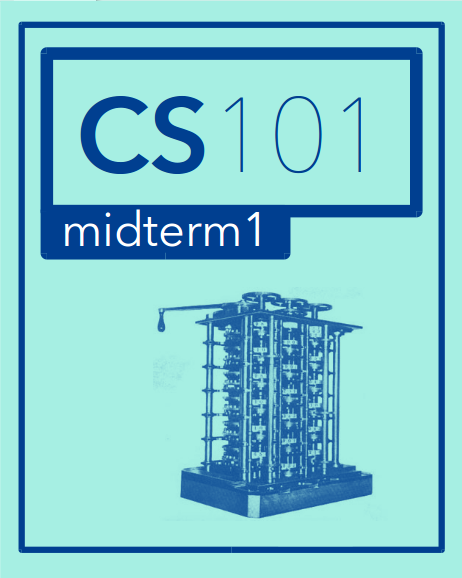
\includegraphics[width=2in]{../img/midterm1-header.png}
\end{center}

\bigskip
\noindent
\begin{itemize}
\item \textbf{Be sure to enter your \underline{NetID} and \underline{the code below} on your Scantron}.
\item Do not turn this page until instructed to do so.
\item There are 30 questions, worth 1 point each.
\item Each question has only \textbf{one} correct answer.
\item You must not communicate with other students during this test.
\item No books, notes, or electronic devices are permitted.
\item This is a 60-minute exam.
\item There are several different versions of this exam.
\end{itemize}

\bigskip\bigskip
\noindent
\textbf{\Large 1. Fill in your information:}

\bigskip
{\Large\bf
\begin{tabular}{ll}
Full Name: & \underbar{\hskip 8cm} \\[0.5em]
UIN (Student Number): & \underbar{\hskip 8cm} \\[0.5em]
NetID: & \underbar{\hskip 8cm}
\end{tabular}
}

\bigskip
\bigskip
\noindent
\textbf{\Large 2. Fill in the following answers on the Scantron form:}

%%%%%%%%%%%%%%%%%%%%%%%%%%%%%%%%%%%%%%%%%%%%%%%%%%%%%%%%%
%%%%%%%%%%%%%%%%%%%%%%%%%%%%%%%%%%%%%%%%%%%%%%%%%%%%%%%%%

\begin{enumerate}
\item[92.] A
\item[93.] C
\item[94.] A
\item[95.] A
\item[96.] B
\end{enumerate}

\newpage

% Zone 1


%%%%%%%%%%%%%%%%%%%%%%%%%%%%%%%%%%%%%%%%%%%%%%%%%%%%%%%%%



\newpage
\noindent
1. (1 point)
Consider the following program:
\begin{verbatim}
def fix(s):
    a=list(s)
    a.sort()
    return ''.join(a)

x=["one","two","eleven","twelve"]
s1=fix(x[0]+x[-1])
s2=fix(x[1]+x[-2])

if s1==s2:
    x.sort()
elif s1<s2:
    x.reverse()
else:
    x.append("six")
\end{verbatim}
What is the \textbf{value} of \texttt{x} after this program is executed?


\begin{enumerate}
\item[(A)]
\begin{verbatim}['two', 'twelve', 'one', 'eleven', 'six']\end{verbatim}

\item[(B)]
\begin{verbatim}['one', 'two', 'eleven', 'twelve']\end{verbatim}

\item[(C)]
\begin{verbatim}['one', 'two', 'eleven', 'twelve', 'six']\end{verbatim}

\item[(D)]
\begin{verbatim}['twelve', 'eleven', 'two', 'one']\end{verbatim}

\item[(E)] $\bigstar$ 
\begin{verbatim}['eleven', 'one', 'twelve', 'two']\end{verbatim}

\end{enumerate}

\vspace*{2em}
\hrule
\vspace{2em}

\noindent {\bf Solution.} 
\vspace{2em}
\hrule height 2pt


\newpage
\noindent
2. (1 point)
Consider the following incomplete function.
\begin{verbatim}
def isdivisible(m,n):
    if ???:
        return False
    else:
        return True
\end{verbatim}
The function is intended to return True if the input parameter m is evenly divisible by the parameter n and False otherwise. For example, \verb|isdivisible(4,2)| should return \verb|True|, but \verb|isdivisible(5,3)| should return \verb|False|. What should replace the three question marks to complete the function?


\begin{enumerate}
\item[(A)] $\bigstar$ 
\begin{verbatim}(m % n) != 0 \end{verbatim}

\item[(B)]
\begin{verbatim}(m // n) != 0 \end{verbatim}

\item[(C)]
\begin{verbatim}(n % m) == 0 \end{verbatim}

\item[(D)]
\begin{verbatim}(n // m) == 0 \end{verbatim}

\end{enumerate}

\vspace*{2em}
\hrule
\vspace{2em}

\noindent {\bf Solution.} 
\vspace{2em}
\hrule height 2pt


\newpage
\noindent
3. (1 point)
Consider the following incomplete Python program.
\begin{verbatim}
s="".join(["2","2","0","1"])
x=0
for i in range(len(s)-1):
    x+=int(???)
\end{verbatim}
What should replace the three question marks so the resulting value of \texttt{x} is 43?


\begin{enumerate}
\item[(A)]
\begin{verbatim}s[i:i-1]\end{verbatim}

\item[(B)]
\begin{verbatim}s[i+1:i+2]\end{verbatim}

\item[(C)]
\begin{verbatim}s[i:i+1]\end{verbatim}

\item[(D)] $\bigstar$ 
\begin{verbatim}s[i:i+2]\end{verbatim}

\end{enumerate}

\vspace*{2em}
\hrule
\vspace{2em}

\noindent {\bf Solution.} 
\vspace{2em}
\hrule height 2pt


\newpage
\noindent
4. (1 point)
Consider the following program:
\begin{verbatim}
x=0
for i in range(2,8):
    if i%3==0:
        x+=3
    elif i%2==0:
        x+=2
    else:
        x+=1
\end{verbatim}
What is the \textbf{value} of \texttt{x} after this program is executed?


\begin{enumerate}
\item[(A)] $\bigstar$ 
\begin{verbatim}12\end{verbatim}

\item[(B)]
\begin{verbatim}11\end{verbatim}

\item[(C)]
\begin{verbatim}14\end{verbatim}

\item[(D)]
\begin{verbatim}10\end{verbatim}

\item[(E)]
\begin{verbatim}13\end{verbatim}

\end{enumerate}

\vspace*{2em}
\hrule
\vspace{2em}

\noindent {\bf Solution.} 
\vspace{2em}
\hrule height 2pt


\newpage
\noindent
5. (1 point)
Consider the following program:
\begin{verbatim}
a=3
b=4
if a==3:
    b=a
elif a==4:
    a=5
else:
    a=b
\end{verbatim}
What is the \textbf{value} of a after this program is executed?


\begin{enumerate}
\item[(A)]
None of the other answers are correct.

\item[(B)] $\bigstar$ 
\begin{verbatim}3\end{verbatim}

\item[(C)]
\begin{verbatim}5\end{verbatim}

\item[(D)]
\begin{verbatim}4\end{verbatim}

\item[(E)]
\begin{verbatim}7\end{verbatim}

\end{enumerate}

\vspace*{2em}
\hrule
\vspace{2em}

\noindent {\bf Solution.} 
\vspace{2em}
\hrule height 2pt


\newpage
\noindent
6. (1 point)
Consider the following program:
\begin{verbatim}
x="KING ARTHUR-MORGANA LEFAY-SIR BEDIVERE".split("-")
y=x
x=y.reverse()
\end{verbatim}
What is the \textbf{value} of \texttt{x} after this program is executed?


\begin{enumerate}
\item[(A)]
\begin{verbatim}['KING', 'ARTHUR-MORGANA', 'LEFAY-SIR', 'BEDIVERE']\end{verbatim}

\item[(B)] $\bigstar$ 
\begin{verbatim}None\end{verbatim}

\item[(C)]
\begin{verbatim}['SIR BEDIVERE', 'MORGANA LEFAY', 'KING ARTHUR']\end{verbatim}

\item[(D)]
\begin{verbatim}['BEDIVERE', 'LEFAY-SIR', 'ARTHUR-MORGANA', 'KING']\end{verbatim}

\item[(E)]
\begin{verbatim}['KING ARTHUR', 'MORGANA LEFAY', 'SIR BEDIVERE']\end{verbatim}

\end{enumerate}

\vspace*{2em}
\hrule
\vspace{2em}

\noindent {\bf Solution.} 
\vspace{2em}
\hrule height 2pt


\newpage
\noindent
7. (1 point)
Consider the following program.
\begin{verbatim}
s="BBCAA"
x=0
y=len(s)-1
while s[x]!=s[y] and x<len(s):
    x+=1
    y-=1
\end{verbatim}
After it is run, what is the final \textbf{value} of \texttt{x}?


\begin{enumerate}
\item[(A)]
\begin{verbatim}0\end{verbatim}

\item[(B)]
\begin{verbatim}3\end{verbatim}

\item[(C)]
\begin{verbatim}1\end{verbatim}

\item[(D)]
\begin{verbatim}4\end{verbatim}

\item[(E)] $\bigstar$ 
\begin{verbatim}2\end{verbatim}

\end{enumerate}

\vspace*{2em}
\hrule
\vspace{2em}

\noindent {\bf Solution.} 
\vspace{2em}
\hrule height 2pt


\newpage
\noindent
8. (1 point)
Consider the following program.
\begin{verbatim}
x=1
i=0
while(x*x)<=9:
    i=i+(x*x)
    x=x+1
\end{verbatim}
After it is run, what is the final \textbf{value} of \texttt{x}?


\begin{enumerate}
\item[(A)]
\begin{verbatim}3\end{verbatim}

\item[(B)]
\begin{verbatim}14\end{verbatim}

\item[(C)]
\begin{verbatim}30\end{verbatim}

\item[(D)]
\begin{verbatim}5\end{verbatim}

\item[(E)] $\bigstar$ 
\begin{verbatim}4\end{verbatim}

\end{enumerate}

\vspace*{2em}
\hrule
\vspace{2em}

\noindent {\bf Solution.} 
\vspace{2em}
\hrule height 2pt


\newpage
\noindent
9. (1 point)
Consider the following program:
\begin{verbatim}
s="ECTOR"
t="GAWAIN"
x=(len(s)+len(t)) < 4 and s in t
\end{verbatim}
What is the \textbf{type} of \texttt{x} after this program is executed?


\begin{enumerate}
\item[(A)]
\begin{verbatim}Float\end{verbatim}

\item[(B)] $\bigstar$ 
\begin{verbatim}Boolean\end{verbatim}

\item[(C)]
\begin{verbatim}None\end{verbatim}

\item[(D)]
\begin{verbatim}Integer\end{verbatim}

\item[(E)]
\begin{verbatim}String\end{verbatim}

\end{enumerate}

\vspace*{2em}
\hrule
\vspace{2em}

\noindent {\bf Solution.} 
\vspace{2em}
\hrule height 2pt


\newpage
\noindent
10. (1 point)
Consider the following program:
\begin{verbatim}
x=[1,2,3]
def f(a):
    s=""
    a.reverse()
    for i in a:
        s+=str(i)
    return s

x.append(f(x))
\end{verbatim}
What is the \textbf{value} of \texttt{x} after this program is executed?


\begin{enumerate}
\item[(A)]
\begin{verbatim}[1, 2, 3, '321']\end{verbatim}

\item[(B)]
\begin{verbatim}[3, 2, 1]\end{verbatim}

\item[(C)]
\begin{verbatim}[1, 2, 3, 6]\end{verbatim}

\item[(D)]
\begin{verbatim}[1, 2, 3]\end{verbatim}

\item[(E)] $\bigstar$ 
\begin{verbatim}[3, 2, 1, '321']\end{verbatim}

\end{enumerate}

\vspace*{2em}
\hrule
\vspace{2em}

\noindent {\bf Solution.} 
\vspace{2em}
\hrule height 2pt


\newpage
\noindent
11. (1 point)
Consider the following program.
\begin{verbatim}
x=[]
for j in range(0,5):
    if (j%3)==0:
        x.append("-")
    if (j%4)==0:
        x.append("*")
\end{verbatim}
After it is run, what is the final \textbf{value} of \texttt{x}?


\begin{enumerate}
\item[(A)]
\begin{verbatim}["*","-","*"]\end{verbatim}

\item[(B)] $\bigstar$ 
\begin{verbatim}["-","*","-","*"]\end{verbatim}

\item[(C)]
\begin{verbatim}["-","*"]\end{verbatim}

\item[(D)]
None of the other answers are correct.

\item[(E)]
\begin{verbatim}["*","-","*"]\end{verbatim}

\end{enumerate}

\vspace*{2em}
\hrule
\vspace{2em}

\noindent {\bf Solution.} 
\vspace{2em}
\hrule height 2pt


\newpage
\noindent
12. (1 point)
Evaluate the following expression:
\begin{verbatim}
len("ABCD"[0:3])
\end{verbatim}
What value is produced?


\begin{enumerate}
\item[(A)] $\bigstar$ 
3

\item[(B)]
4

\item[(C)]
1

\item[(D)]
2

\end{enumerate}

\vspace*{2em}
\hrule
\vspace{2em}

\noindent {\bf Solution.} 
\vspace{2em}
\hrule height 2pt


\newpage
\noindent
13. (1 point)
Consider the following program.
\begin{verbatim}
def artificing(s):
    return s*2
    return s+"%i" % 2
    return s

s=artificing("MERLIN")
\end{verbatim}
After it is run, what is the final \textbf{value} of s?


\begin{enumerate}
\item[(A)]
\begin{verbatim}None\end{verbatim}

\item[(B)]
\begin{verbatim}"MERLIN2"\end{verbatim}

\item[(C)]
\begin{verbatim}12\end{verbatim}

\item[(D)]
\begin{verbatim}"MERLIN"\end{verbatim}

\item[(E)] $\bigstar$ 
\begin{verbatim}"MERLINMERLIN"\end{verbatim}

\end{enumerate}

\vspace*{2em}
\hrule
\vspace{2em}

\noindent {\bf Solution.} 
\vspace{2em}
\hrule height 2pt


\newpage
\noindent
14. (1 point)
Evaluate the following expression:
\begin{verbatim}
[1,2]*len("3")
\end{verbatim}
What value is produced?


\begin{enumerate}
\item[(A)]
\begin{verbatim}[1,2,1]\end{verbatim}

\item[(B)]
\begin{verbatim}[1,2,3]\end{verbatim}

\item[(C)]
\begin{verbatim}[1,2,1,2,1,2]\end{verbatim}

\item[(D)] $\bigstar$ 
\begin{verbatim}[1,2]\end{verbatim}

\end{enumerate}

\vspace*{2em}
\hrule
\vspace{2em}

\noindent {\bf Solution.} 
\vspace{2em}
\hrule height 2pt


\newpage
\noindent
15. (1 point)
Consider the following program.
\begin{verbatim}
kay = 2
wart = 3

def knight(kay,wart):
    wart += 2
    kay += 3
    return wart + kay

wart = knight(kay, kay) + knight(wart, wart)
\end{verbatim}
After it is run, what is the final \textbf{value} of \texttt{wart}?


\begin{enumerate}
\item[(A)]
\begin{verbatim}5\end{verbatim}

\item[(B)]
\begin{verbatim}2\end{verbatim}

\item[(C)] $\bigstar$ 
None of the other answers are correct.

\item[(D)]
\begin{verbatim}3\end{verbatim}

\end{enumerate}

\vspace*{2em}
\hrule
\vspace{2em}

\noindent {\bf Solution.} 
\vspace{2em}
\hrule height 2pt


\newpage
\noindent
16. (1 point)
For this problem, you should compose a function which accomplishes a given task using the available code blocks arranged in the correct functional order.  \emph{We ignore indentation for this problem.}

\texttt{find\_max} should accept a \texttt{list} and return the value of the maximum item in the \texttt{list}.  (\texttt{None} is always the lowest value in any numeric comparison, so you may use it as an initializer.)

\begin{verbatim}
def find_max(my_list):
\end{verbatim}

\begin{enumerate}[1]
\item \texttt{max\_val = i}
\item \texttt{max\_val = None}
\item \texttt{for i in range(len(my\_list)):}
\item \texttt{if i > max\_val:}
\item \texttt{max\_val = my\_list[i]}
\item \texttt{return max\_val}
\item \texttt{for i in range(my\_list):}
\item \texttt{if my\_list[i] > max\_val:}
\item \texttt{print(max\_val)}
\end{enumerate}



\begin{enumerate}
\item[(A)]
2, 7, 4, 5, 6

\item[(B)] $\bigstar$ 
2, 3, 8, 5, 6

\item[(C)]
2, 3, 4, 1, 6

\item[(D)]
2, 3, 8, 1, 6

\item[(E)]
3, 2, 8, 5, 9

\end{enumerate}

\vspace*{2em}
\hrule
\vspace{2em}

\noindent {\bf Solution.} 
\vspace{2em}
\hrule height 2pt


\newpage
\noindent
17. (1 point)
Consider the following program:
\begin{verbatim}
a=["S","T","U","P","E","F","Y"]
a=a[0:4]
a.sort()
x=""
for e in a:
    x=e+x
\end{verbatim}
What is the \textbf{value} of \texttt{x} after this program is executed?


\begin{enumerate}
\item[(A)]
None of the other answers are correct.

\item[(B)]
\begin{verbatim}"STUP"\end{verbatim}

\item[(C)] $\bigstar$ 
\begin{verbatim}"UTSP"\end{verbatim}

\item[(D)]
\begin{verbatim}"PUST"\end{verbatim}

\item[(E)]
\begin{verbatim}"PSTU"\end{verbatim}

\end{enumerate}

\vspace*{2em}
\hrule
\vspace{2em}

\noindent {\bf Solution.} 
\vspace{2em}
\hrule height 2pt


\newpage
\noindent
18. (1 point)
How can the following mathematical equation be implemented as a Python expression? Assume \verb|a|, \verb|b|, and \verb|cos| have already been defined.
$$a^b \cos(a - b)$$


\begin{enumerate}
\item[(A)]
None of the other answers are correct.

\item[(B)]
\begin{verbatim}(b^a)cos(a-b)\end{verbatim}

\item[(C)]
\begin{verbatim}(a**b)cos(a-b)\end{verbatim}

\item[(D)]
\begin{verbatim}(a^b)*cos(a-b)\end{verbatim}

\item[(E)] $\bigstar$ 
\begin{verbatim}(a**b)*cos(a-b)\end{verbatim}

\end{enumerate}

\vspace*{2em}
\hrule
\vspace{2em}

\noindent {\bf Solution.} 
\vspace{2em}
\hrule height 2pt


\newpage
\noindent
19. (1 point)
Consider the following program:
\begin{verbatim}
pi="3.14159"
e="2.71828"
x=(float(e)**float(pi)-float(pi)) == 20
\end{verbatim}
What is the \textbf{type} of \texttt{x} after this program is executed?


\begin{enumerate}
\item[(A)]
\begin{verbatim}Float\end{verbatim}

\item[(B)]
\begin{verbatim}Integer\end{verbatim}

\item[(C)] $\bigstar$ 
\begin{verbatim}Boolean\end{verbatim}

\item[(D)]
\begin{verbatim}String\end{verbatim}

\item[(E)]
\begin{verbatim}None\end{verbatim}

\end{enumerate}

\vspace*{2em}
\hrule
\vspace{2em}

\noindent {\bf Solution.} 
\vspace{2em}
\hrule height 2pt


\newpage
\noindent
20. (1 point)
Consider the following Python program.
\begin{verbatim}
e=[1,3,5,7,9,11]
d=[0,0,0]
for i in range(0,len(e)):
    d[i%3]+=e[i]
x=d[2]
\end{verbatim}
After it is run, what is the final \textbf{value} of \texttt{x}?


\begin{enumerate}
\item[(A)]
\begin{verbatim}7\end{verbatim}

\item[(B)]
\begin{verbatim}12\end{verbatim}

\item[(C)]
\begin{verbatim}0\end{verbatim}

\item[(D)]
\begin{verbatim}8\end{verbatim}

\item[(E)] $\bigstar$ 
\begin{verbatim}16\end{verbatim}

\end{enumerate}

\vspace*{2em}
\hrule
\vspace{2em}

\noindent {\bf Solution.} 
\vspace{2em}
\hrule height 2pt


\newpage
\noindent
21. (1 point)
What is the result of the following expression?
\begin{verbatim}
[ 1, 2, 3 ] * 3
\end{verbatim}


\begin{enumerate}
\item[(A)]
\begin{verbatim}[3.0, 6.0, 9.0]\end{verbatim}

\item[(B)]
\begin{verbatim}[3, 6, 9]\end{verbatim}

\item[(C)]
\begin{verbatim}[1.0, 2.0, 3.0, 1.0, 2.0, 3.0, 1.0, 2.0, 3.0]\end{verbatim}

\item[(D)]
\begin{verbatim}(3, 6, 9)\end{verbatim}

\item[(E)] $\bigstar$ 
\begin{verbatim}[1, 2, 3, 1, 2, 3, 1, 2, 3]\end{verbatim}

\end{enumerate}

\vspace*{2em}
\hrule
\vspace{2em}

\noindent {\bf Solution.} 
\vspace{2em}
\hrule height 2pt


\newpage
\noindent
22. (1 point)
Consider the following program:
\begin{verbatim}
x=[1,2,3,4,5,6,7,8,9]
x=x[2:-2]
i=1
while i < 3:
    x[i]+=1
    i+=1
\end{verbatim}
What is the \textbf{value} of \texttt{x} after this program is executed?


\begin{enumerate}
\item[(A)]
\begin{verbatim}[2, 4, 5, 6, 6, 7]\end{verbatim}

\item[(B)]
\begin{verbatim}[3, 5, 6, 6, 7, 8]\end{verbatim}

\item[(C)]
\begin{verbatim}[2, 4, 5, 5, 6, 7]\end{verbatim}

\item[(D)] $\bigstar$ 
\begin{verbatim}[3, 5, 6, 6, 7]\end{verbatim}

\item[(E)]
\begin{verbatim}[3, 5, 6, 6]\end{verbatim}

\end{enumerate}

\vspace*{2em}
\hrule
\vspace{2em}

\noindent {\bf Solution.} 
\vspace{2em}
\hrule height 2pt


\newpage
\noindent
23. (1 point)
Consider the following program:
\begin{verbatim}
s="Hobbes"
i=0
x=-1
while i<len(s):
    if s[i]=='b':
        x=i
    i+=1
\end{verbatim}
What is the \textbf{value} of \texttt{x} after this program is executed?


\begin{enumerate}
\item[(A)]
\begin{verbatim}-1\end{verbatim}

\item[(B)]
\begin{verbatim}4\end{verbatim}

\item[(C)]
\begin{verbatim}5\end{verbatim}

\item[(D)]
\begin{verbatim}2\end{verbatim}

\item[(E)] $\bigstar$ 
\begin{verbatim}3\end{verbatim}

\end{enumerate}

\vspace*{2em}
\hrule
\vspace{2em}

\noindent {\bf Solution.} 
\vspace{2em}
\hrule height 2pt


\newpage
\noindent
24. (1 point)
Consider the following program:
\begin{verbatim}
a=["merlin","sir agravaine","king pellinore"]
b=[ ]
for i in range(0,4):
    b.append(a[0-i].title())
\end{verbatim}
What is the \textbf{value} of b after this program is executed?


\begin{enumerate}
\item[(A)]
\begin{verbatim}['Merlin', 'Sir Agravaine', 'King Pellinore', 'Merlin']\end{verbatim}

\item[(B)]
\begin{verbatim}['Merlin', 'King Pellinore', 'Sir Agravaine']\end{verbatim}

\item[(C)]
\begin{verbatim}[ ]\end{verbatim}

\item[(D)] $\bigstar$ 
\begin{verbatim}['Merlin', 'King Pellinore', 'Sir Agravaine', 'Merlin']\end{verbatim}

\item[(E)]
\begin{verbatim}['King Pellinore', 'Sir Agravaine', 'Merlin']\end{verbatim}

\end{enumerate}

\vspace*{2em}
\hrule
\vspace{2em}

\noindent {\bf Solution.} 
\vspace{2em}
\hrule height 2pt


\newpage
\noindent
25. (1 point)
Consider the following program:
\begin{verbatim}
i=3
x=2
while i < 7:
    x+=i
    i+=2
\end{verbatim}
What is the \textbf{value} of \texttt{x} after this program is executed?


\begin{enumerate}
\item[(A)] $\bigstar$ 
\begin{verbatim}10\end{verbatim}

\item[(B)]
\begin{verbatim}13\end{verbatim}

\item[(C)]
\begin{verbatim}12\end{verbatim}

\item[(D)]
\begin{verbatim}11\end{verbatim}

\item[(E)]
\begin{verbatim}14\end{verbatim}

\end{enumerate}

\vspace*{2em}
\hrule
\vspace{2em}

\noindent {\bf Solution.} 
\vspace{2em}
\hrule height 2pt


\newpage
\noindent
26. (1 point)
Consider the following program:
\begin{verbatim}
s="G+R+A+I+L"
x=s.split("+")[1:-2]
\end{verbatim}
What is the \textbf{value} of \texttt{x} after this program is executed?


\begin{enumerate}
\item[(A)]
\begin{verbatim}None\end{verbatim}

\item[(B)] $\bigstar$ 
\begin{verbatim}['R','A']\end{verbatim}

\item[(C)]
\begin{verbatim}False\end{verbatim}

\item[(D)]
\begin{verbatim}3\end{verbatim}

\item[(E)]
\begin{verbatim}'RAI'\end{verbatim}

\end{enumerate}

\vspace*{2em}
\hrule
\vspace{2em}

\noindent {\bf Solution.} 
\vspace{2em}
\hrule height 2pt


\newpage
\noindent
27. (1 point)
Consider the following incomplete program.
\begin{verbatim}
sum=0
for i in range(0,100):
    ???

\end{verbatim}
The program is intended to sum all of the integers between 1 and 100 (inclusive). What should replace the three question marks to complete the program?


\begin{enumerate}
\item[(A)]
\begin{verbatim}sum=sum+i \end{verbatim}

\item[(B)]
\begin{verbatim}sum=sum+1\end{verbatim}

\item[(C)]
\begin{verbatim}sum+1=sum \end{verbatim}

\item[(D)] $\bigstar$ 
\begin{verbatim}sum=sum+i+1 \end{verbatim}

\end{enumerate}

\vspace*{2em}
\hrule
\vspace{2em}

\noindent {\bf Solution.} 
\vspace{2em}
\hrule height 2pt


\newpage
\noindent
28. (1 point)
Consider the following program:
\begin{verbatim}
s="TRIS %i"
t="ISEU"
x=len(s) % len(t[2:-1])
\end{verbatim}
What is the \textbf{type} of \texttt{x} after this program is executed?


\begin{enumerate}
\item[(A)] $\bigstar$ 
\begin{verbatim}Integer\end{verbatim}

\item[(B)]
\begin{verbatim}Float\end{verbatim}

\item[(C)]
\begin{verbatim}String\end{verbatim}

\item[(D)]
\begin{verbatim}None\end{verbatim}

\item[(E)]
\begin{verbatim}Boolean\end{verbatim}

\end{enumerate}

\vspace*{2em}
\hrule
\vspace{2em}

\noindent {\bf Solution.} 
\vspace{2em}
\hrule height 2pt


\newpage
\noindent
29. (1 point)
\begin{verbatim}
x=str(3)+"str(3)"
\end{verbatim}
What is the \textbf{value} of \texttt{x} after this program is executed?


\begin{enumerate}
\item[(A)] $\bigstar$ 
\begin{verbatim}"3str(3)"\end{verbatim}

\item[(B)]
\begin{verbatim}"33"\end{verbatim}

\item[(C)]
None of the other answers are correct.

\item[(D)]
\begin{verbatim}"333"\end{verbatim}

\item[(E)]
\begin{verbatim}33\end{verbatim}

\end{enumerate}

\vspace*{2em}
\hrule
\vspace{2em}

\noindent {\bf Solution.} 
\vspace{2em}
\hrule height 2pt


\newpage
\noindent
30. (1 point)
Consider the following program:
\begin{verbatim}
x=2
a=6
if (a%3)==2:
    x=x**3
elif(a%3)==1:
    x=x**2
else:
    x=x**1
\end{verbatim}
What is the \textbf{value} of \texttt{x} after this program is executed?


\begin{enumerate}
\item[(A)]
None of the other answers are correct.

\item[(B)]
\begin{verbatim}8\end{verbatim}

\item[(C)]
\begin{verbatim}16\end{verbatim}

\item[(D)] $\bigstar$ 
\begin{verbatim}2\end{verbatim}

\item[(E)]
\begin{verbatim}4\end{verbatim}

\end{enumerate}

\vspace*{2em}
\hrule
\vspace{2em}

\noindent {\bf Solution.} 
\vspace{2em}
\hrule height 2pt

%%%%%%%%%%%%%%%%%%%%%%%%%%%%%%%%%%%%%%%%%%%%%%%%%%%%%%%%%%%%%%%%%%%%%%
%%%%%%%%%%%%%%%%%%%%%%%%%%%%%%%%%%%%%%%%%%%%%%%%%%%%%%%%%%%%%%%%%%%%%%
%%%%%%%%%%%%%%%%%%%%%%%%%%%%%%%%%%%%%%%%%%%%%%%%%%%%%%%%%%%%%%%%%%%%%%
%%%%%%%%%%%%%%%%%%%%%%%%%%%%%%%%%%%%%%%%%%%%%%%%%%%%%%%%%%%%%%%%%%%%%%
% Exam number 12

\message{Exam 12/50}
\cleardoublepage
\setcounter{page}{1}


\begin{center}
%\textbf{\Large CS 101 Midterm \#1}
%
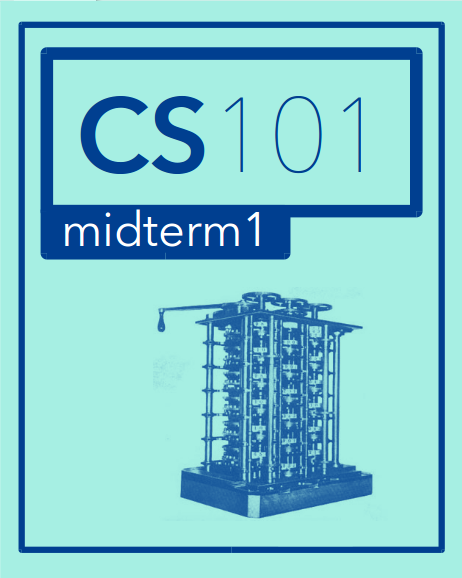
\includegraphics[width=2in]{../img/midterm1-header.png}
\end{center}

\bigskip
\noindent
\begin{itemize}
\item \textbf{Be sure to enter your \underline{NetID} and \underline{the code below} on your Scantron}.
\item Do not turn this page until instructed to do so.
\item There are 30 questions, worth 1 point each.
\item Each question has only \textbf{one} correct answer.
\item You must not communicate with other students during this test.
\item No books, notes, or electronic devices are permitted.
\item This is a 60-minute exam.
\item There are several different versions of this exam.
\end{itemize}

\bigskip\bigskip
\noindent
\textbf{\Large 1. Fill in your information:}

\bigskip
{\Large\bf
\begin{tabular}{ll}
Full Name: & \underbar{\hskip 8cm} \\[0.5em]
UIN (Student Number): & \underbar{\hskip 8cm} \\[0.5em]
NetID: & \underbar{\hskip 8cm}
\end{tabular}
}

\bigskip
\bigskip
\noindent
\textbf{\Large 2. Fill in the following answers on the Scantron form:}

%%%%%%%%%%%%%%%%%%%%%%%%%%%%%%%%%%%%%%%%%%%%%%%%%%%%%%%%%
%%%%%%%%%%%%%%%%%%%%%%%%%%%%%%%%%%%%%%%%%%%%%%%%%%%%%%%%%

\begin{enumerate}
\item[92.] B
\item[93.] C
\item[94.] A
\item[95.] B
\item[96.] C
\end{enumerate}

\newpage

% Zone 1


%%%%%%%%%%%%%%%%%%%%%%%%%%%%%%%%%%%%%%%%%%%%%%%%%%%%%%%%%



\newpage
\noindent
1. (1 point)
Consider the following program:
\begin{verbatim}
a=["A","C","C","I","O"]
a.sort()
a[0]=a[-1]
x=""
for e in a:
    x=x+e
\end{verbatim}
What is the \textbf{value} of \texttt{x} after this program is executed?


\begin{enumerate}
\item[(A)] $\bigstar$ 
\begin{verbatim}"OCCIO"\end{verbatim}

\item[(B)]
\begin{verbatim}"ACCOA"\end{verbatim}

\item[(C)]
None of the other answers are correct.

\item[(D)]
\begin{verbatim}"ACCIA"\end{verbatim}

\item[(E)]
\begin{verbatim}"ICCOI"\end{verbatim}

\end{enumerate}

\vspace*{2em}
\hrule
\vspace{2em}

\noindent {\bf Solution.} 
\vspace{2em}
\hrule height 2pt


\newpage
\noindent
2. (1 point)
Consider the following program:
\begin{verbatim}
x="KING ARTHUR-MORGANA LEFAY-SIR BEDIVERE".split("-")
y=x
x=y.reverse()
\end{verbatim}
What is the \textbf{value} of \texttt{x} after this program is executed?


\begin{enumerate}
\item[(A)]
\begin{verbatim}['SIR BEDIVERE', 'MORGANA LEFAY', 'KING ARTHUR']\end{verbatim}

\item[(B)]
\begin{verbatim}['KING', 'ARTHUR-MORGANA', 'LEFAY-SIR', 'BEDIVERE']\end{verbatim}

\item[(C)]
\begin{verbatim}['KING ARTHUR', 'MORGANA LEFAY', 'SIR BEDIVERE']\end{verbatim}

\item[(D)] $\bigstar$ 
\begin{verbatim}None\end{verbatim}

\item[(E)]
\begin{verbatim}['BEDIVERE', 'LEFAY-SIR', 'ARTHUR-MORGANA', 'KING']\end{verbatim}

\end{enumerate}

\vspace*{2em}
\hrule
\vspace{2em}

\noindent {\bf Solution.} 
\vspace{2em}
\hrule height 2pt


\newpage
\noindent
3. (1 point)
Consider the following program:
\begin{verbatim}
pi="3.14159"
e="2.71828"
x=(float(e)**float(pi)-float(pi)) == 20
\end{verbatim}
What is the \textbf{type} of \texttt{x} after this program is executed?


\begin{enumerate}
\item[(A)] $\bigstar$ 
\begin{verbatim}Boolean\end{verbatim}

\item[(B)]
\begin{verbatim}String\end{verbatim}

\item[(C)]
\begin{verbatim}Integer\end{verbatim}

\item[(D)]
\begin{verbatim}Float\end{verbatim}

\item[(E)]
\begin{verbatim}None\end{verbatim}

\end{enumerate}

\vspace*{2em}
\hrule
\vspace{2em}

\noindent {\bf Solution.} 
\vspace{2em}
\hrule height 2pt


\newpage
\noindent
4. (1 point)
Consider the following incomplete program.
\begin{verbatim}
sum=0
for i in range(0,100):
    ???

\end{verbatim}
The program is intended to sum all of the integers between 1 and 100 (inclusive). What should replace the three question marks to complete the program?


\begin{enumerate}
\item[(A)] $\bigstar$ 
\begin{verbatim}sum=sum+i+1 \end{verbatim}

\item[(B)]
\begin{verbatim}sum=sum+i \end{verbatim}

\item[(C)]
\begin{verbatim}sum=sum+1\end{verbatim}

\item[(D)]
\begin{verbatim}sum+1=sum \end{verbatim}

\end{enumerate}

\vspace*{2em}
\hrule
\vspace{2em}

\noindent {\bf Solution.} 
\vspace{2em}
\hrule height 2pt


\newpage
\noindent
5. (1 point)
Consider the following program.
\begin{verbatim}
x=[]
for j in range(0,5):
    if (j%2)==0:
        x.append("-")
    if (j%5)==0:
        x.append("*")
\end{verbatim}
After it is run, what is the final \textbf{value} of \texttt{x}?


\begin{enumerate}
\item[(A)] $\bigstar$ 
\begin{verbatim}["-","*","-","-"]\end{verbatim}

\item[(B)]
\begin{verbatim}["*","-","*","*"]\end{verbatim}

\item[(C)]
\begin{verbatim}["-","-","*"]\end{verbatim}

\item[(D)]
\begin{verbatim}["-","*","-"]\end{verbatim}

\item[(E)]
None of the other answers are correct.

\end{enumerate}

\vspace*{2em}
\hrule
\vspace{2em}

\noindent {\bf Solution.} 
\vspace{2em}
\hrule height 2pt


\newpage
\noindent
6. (1 point)
Consider the following program:
\begin{verbatim}
x=[1,2,3]
def f(a):
    s=""
    a.append(4)
    for i in a:
        s+=str(i)
    return s

x.append(f(x))
\end{verbatim}
What is the \textbf{value} of \texttt{x} after this program is executed?


\begin{enumerate}
\item[(A)]
\begin{verbatim}[1, 2, 3]\end{verbatim}

\item[(B)]
\begin{verbatim}[1, 2, 3, '1234']\end{verbatim}

\item[(C)] $\bigstar$ 
\begin{verbatim}[1, 2, 3, 4, '1234']\end{verbatim}

\item[(D)]
\begin{verbatim}[1, 2, 3, 10]\end{verbatim}

\item[(E)]
\begin{verbatim}[1, 2, 3, '123']\end{verbatim}

\end{enumerate}

\vspace*{2em}
\hrule
\vspace{2em}

\noindent {\bf Solution.} 
\vspace{2em}
\hrule height 2pt


\newpage
\noindent
7. (1 point)
Consider the following program:
\begin{verbatim}
a=["merlin","sir agravaine","king pellinore"]
b=[ ]
for i in range(1,3):
    b.append(a[0-i].title())
\end{verbatim}
What is the \textbf{value} of b after this program is executed?


\begin{enumerate}
\item[(A)] $\bigstar$ 
\begin{verbatim}['King Pellinore', 'Sir Agravaine']\end{verbatim}

\item[(B)]
\begin{verbatim}['Sir Agravaine', 'King Pellinore']\end{verbatim}

\item[(C)]
\begin{verbatim}[ ]\end{verbatim}

\item[(D)]
\begin{verbatim}['Merlin', 'King Pellinore', 'Sir Agravaine']\end{verbatim}

\item[(E)]
\begin{verbatim}['King Pellinore', 'Sir Agravaine', 'Merlin']\end{verbatim}

\end{enumerate}

\vspace*{2em}
\hrule
\vspace{2em}

\noindent {\bf Solution.} 
\vspace{2em}
\hrule height 2pt


\newpage
\noindent
8. (1 point)
Consider the following program:
\begin{verbatim}
def fix(s):
    a=list(s)
    a.sort()
    return ''.join(a)

x=["one","two","eleven","twelve"]
s1=fix(x[0]+x[-1])
s2=fix(x[1]+x[-2])

if s1<s2:
    x.sort()
elif s1==s2:
    x.reverse()
else:
    x.append("six")
\end{verbatim}
What is the \textbf{value} of \texttt{x} after this program is executed?


\begin{enumerate}
\item[(A)] $\bigstar$ 
\begin{verbatim}['twelve', 'eleven', 'two', 'one']\end{verbatim}

\item[(B)]
\begin{verbatim}['one', 'two', 'eleven', 'twelve']\end{verbatim}

\item[(C)]
\begin{verbatim}['eleven', 'one', 'twelve', 'two']\end{verbatim}

\item[(D)]
\begin{verbatim}['two', 'twelve', 'one', 'eleven', 'six']\end{verbatim}

\item[(E)]
\begin{verbatim}['one', 'two', 'eleven', 'twelve', 'six']\end{verbatim}

\end{enumerate}

\vspace*{2em}
\hrule
\vspace{2em}

\noindent {\bf Solution.} 
\vspace{2em}
\hrule height 2pt


\newpage
\noindent
9. (1 point)
Consider the following program:
\begin{verbatim}
a=3
b=4
if a==3:
    a=b
elif a==4:
    a=5
else:
    b=a
\end{verbatim}
What is the \textbf{value} of a after this program is executed?


\begin{enumerate}
\item[(A)]
None of the other answers are correct.

\item[(B)]
\begin{verbatim}7\end{verbatim}

\item[(C)] $\bigstar$ 
\begin{verbatim}4\end{verbatim}

\item[(D)]
\begin{verbatim}3\end{verbatim}

\item[(E)]
\begin{verbatim}5\end{verbatim}

\end{enumerate}

\vspace*{2em}
\hrule
\vspace{2em}

\noindent {\bf Solution.} 
\vspace{2em}
\hrule height 2pt


\newpage
\noindent
10. (1 point)
Consider the following program:
\begin{verbatim}
s="ECTOR"
t="GAWAIN"
x=(len(s)+len(t)) < 4 and s in t
\end{verbatim}
What is the \textbf{type} of \texttt{x} after this program is executed?


\begin{enumerate}
\item[(A)]
\begin{verbatim}Integer\end{verbatim}

\item[(B)]
\begin{verbatim}None\end{verbatim}

\item[(C)] $\bigstar$ 
\begin{verbatim}Boolean\end{verbatim}

\item[(D)]
\begin{verbatim}String\end{verbatim}

\item[(E)]
\begin{verbatim}Float\end{verbatim}

\end{enumerate}

\vspace*{2em}
\hrule
\vspace{2em}

\noindent {\bf Solution.} 
\vspace{2em}
\hrule height 2pt


\newpage
\noindent
11. (1 point)
Consider the following incomplete Python program.
\begin{verbatim}
s="".join(["0","1","2","1"])
x=0
for i in range(len(s)-1):
    x+=int(???)
\end{verbatim}
What should replace the three question marks so the resulting value of \texttt{x} is 34?


\begin{enumerate}
\item[(A)]
\begin{verbatim}s[i+1:i+2]\end{verbatim}

\item[(B)]
\begin{verbatim}s[i:i-1]\end{verbatim}

\item[(C)] $\bigstar$ 
\begin{verbatim}s[i:i+2]\end{verbatim}

\item[(D)]
\begin{verbatim}s[i:i+1]\end{verbatim}

\end{enumerate}

\vspace*{2em}
\hrule
\vspace{2em}

\noindent {\bf Solution.} 
\vspace{2em}
\hrule height 2pt


\newpage
\noindent
12. (1 point)
Consider the following program:
\begin{verbatim}
x=[2,3,4,5,6,7,8,9]
x=x[2:-2]
i=1
while i <= 3:
    x[i]+=1
    i+=1
\end{verbatim}
What is the \textbf{value} of \texttt{x} after this program is executed?


\begin{enumerate}
\item[(A)]
\begin{verbatim}[2, 4, 6, 6]\end{verbatim}

\item[(B)]
\begin{verbatim}[4, 6, 7]\end{verbatim}

\item[(C)] $\bigstar$ 
\begin{verbatim}[4, 6, 7, 8]\end{verbatim}

\item[(D)]
\begin{verbatim}[4, 6, 7, 7]\end{verbatim}

\item[(E)]
\begin{verbatim}[3, 4, 6, 7, 8]\end{verbatim}

\end{enumerate}

\vspace*{2em}
\hrule
\vspace{2em}

\noindent {\bf Solution.} 
\vspace{2em}
\hrule height 2pt


\newpage
\noindent
13. (1 point)
Consider the following Python program.
\begin{verbatim}
e=[1,3,5,7,9,11]
d=[0,0,0]
for i in range(0,len(e)):
    d[i%3]+=e[i]
x=d[2]
\end{verbatim}
After it is run, what is the final \textbf{value} of \texttt{x}?


\begin{enumerate}
\item[(A)] $\bigstar$ 
\begin{verbatim}16\end{verbatim}

\item[(B)]
\begin{verbatim}8\end{verbatim}

\item[(C)]
\begin{verbatim}7\end{verbatim}

\item[(D)]
\begin{verbatim}0\end{verbatim}

\item[(E)]
\begin{verbatim}12\end{verbatim}

\end{enumerate}

\vspace*{2em}
\hrule
\vspace{2em}

\noindent {\bf Solution.} 
\vspace{2em}
\hrule height 2pt


\newpage
\noindent
14. (1 point)
What is the result of the following expression?
\begin{verbatim}
[ 1, 2, 3 ] * 3.0
\end{verbatim}


\begin{enumerate}
\item[(A)]
\begin{verbatim}[1.0, 2.0, 3.0, 1.0, 2.0, 3.0, 1.0, 2.0, 3.0]\end{verbatim}

\item[(B)] $\bigstar$ 
\begin{verbatim}[1, 2, 3, 1, 2, 3, 1, 2, 3]\end{verbatim}

\item[(C)]
\begin{verbatim}[3.0, 6.0, 9.0]\end{verbatim}

\item[(D)]
\begin{verbatim}None of the above.\end{verbatim}

\item[(E)]
\begin{verbatim}[3, 6, 9]\end{verbatim}

\end{enumerate}

\vspace*{2em}
\hrule
\vspace{2em}

\noindent {\bf Solution.} 
\vspace{2em}
\hrule height 2pt


\newpage
\noindent
15. (1 point)
Consider the following program:
\begin{verbatim}
s="Calvin"
i=0
x=-1
while i<len(s):
    if s[i]=='b':
        x=i
    i+=1
\end{verbatim}
What is the \textbf{value} of \texttt{x} after this program is executed?


\begin{enumerate}
\item[(A)]
\begin{verbatim}5\end{verbatim}

\item[(B)] $\bigstar$ 
\begin{verbatim}-1\end{verbatim}

\item[(C)]
\begin{verbatim}0\end{verbatim}

\item[(D)]
\begin{verbatim}6\end{verbatim}

\item[(E)]
\begin{verbatim}3\end{verbatim}

\end{enumerate}

\vspace*{2em}
\hrule
\vspace{2em}

\noindent {\bf Solution.} 
\vspace{2em}
\hrule height 2pt


\newpage
\noindent
16. (1 point)
For this problem, you should compose a function which accomplishes a given task using the available code blocks arranged in the correct functional order.  \emph{We ignore indentation for this problem.}

\texttt{find\_max} should accept a \texttt{list} and return the value of the maximum item in the \texttt{list}.  (\texttt{None} is always the lowest value in any numeric comparison, so you may use it as an initializer.)

\begin{verbatim}
def find_max(my_list):
\end{verbatim}

\begin{enumerate}[1]
\item \texttt{max\_val = i}
\item \texttt{max\_val = None}
\item \texttt{for i in range(len(my\_list)):}
\item \texttt{if i > max\_val:}
\item \texttt{max\_val = my\_list[i]}
\item \texttt{return max\_val}
\item \texttt{for i in range(my\_list):}
\item \texttt{if my\_list[i] > max\_val:}
\item \texttt{print(max\_val)}
\end{enumerate}



\begin{enumerate}
\item[(A)]
2, 7, 4, 5, 6

\item[(B)] $\bigstar$ 
2, 3, 8, 5, 6

\item[(C)]
2, 3, 8, 1, 6

\item[(D)]
2, 3, 4, 1, 6

\item[(E)]
3, 2, 8, 5, 9

\end{enumerate}

\vspace*{2em}
\hrule
\vspace{2em}

\noindent {\bf Solution.} 
\vspace{2em}
\hrule height 2pt


\newpage
\noindent
17. (1 point)
Evaluate the following expression:
\begin{verbatim}
len("ABCDE"[1:4])
\end{verbatim}
What value is produced?


\begin{enumerate}
\item[(A)]
5

\item[(B)]
1

\item[(C)] $\bigstar$ 
3

\item[(D)]
4

\end{enumerate}

\vspace*{2em}
\hrule
\vspace{2em}

\noindent {\bf Solution.} 
\vspace{2em}
\hrule height 2pt


\newpage
\noindent
18. (1 point)
How can the following mathematical equation be implemented as a Python expression? Assume \verb|a|, \verb|b|, and \verb|sin| have already been defined.
$$a \sin(a^b - b)$$


\begin{enumerate}
\item[(A)]
\begin{verbatim}a*sin(a^b - b)\end{verbatim}

\item[(B)]
\begin{verbatim}a sin(a**b - b)\end{verbatim}

\item[(C)] $\bigstar$ 
\begin{verbatim}a*sin(a**b - b)\end{verbatim}

\item[(D)]
None of the other answers are correct.

\item[(E)]
\begin{verbatim}a*sin(b^a - b)\end{verbatim}

\end{enumerate}

\vspace*{2em}
\hrule
\vspace{2em}

\noindent {\bf Solution.} 
\vspace{2em}
\hrule height 2pt


\newpage
\noindent
19. (1 point)
Consider the following program:
\begin{verbatim}
s="TRIS %i"
t="ISEU"
x=len(s) % len(t[2:-1])
\end{verbatim}
What is the \textbf{type} of \texttt{x} after this program is executed?


\begin{enumerate}
\item[(A)] $\bigstar$ 
\begin{verbatim}Integer\end{verbatim}

\item[(B)]
\begin{verbatim}Boolean\end{verbatim}

\item[(C)]
\begin{verbatim}String\end{verbatim}

\item[(D)]
\begin{verbatim}Float\end{verbatim}

\item[(E)]
\begin{verbatim}None\end{verbatim}

\end{enumerate}

\vspace*{2em}
\hrule
\vspace{2em}

\noindent {\bf Solution.} 
\vspace{2em}
\hrule height 2pt


\newpage
\noindent
20. (1 point)
Consider the following program:
\begin{verbatim}
x=3
a=5
if (a%3)==2:
    x=x**3
elif(a%3)==1:
    x=x**2
else:
    x=x**1
\end{verbatim}
What is the \textbf{value} of \texttt{x} after this program is executed?


\begin{enumerate}
\item[(A)]
None of the other answers are correct.

\item[(B)] $\bigstar$ 
\begin{verbatim}27\end{verbatim}

\item[(C)]
\begin{verbatim}1\end{verbatim}

\item[(D)]
\begin{verbatim}3\end{verbatim}

\item[(E)]
\begin{verbatim}9\end{verbatim}

\end{enumerate}

\vspace*{2em}
\hrule
\vspace{2em}

\noindent {\bf Solution.} 
\vspace{2em}
\hrule height 2pt


\newpage
\noindent
21. (1 point)
Consider the following program.
\begin{verbatim}
x=0
i=1
while(i*i)<=9:
    x=x+(i*i)
    i=i+1
\end{verbatim}
After it is run, what is the final \textbf{value} of \texttt{x}?


\begin{enumerate}
\item[(A)] $\bigstar$ 
\begin{verbatim}14\end{verbatim}

\item[(B)]
\begin{verbatim}5\end{verbatim}

\item[(C)]
\begin{verbatim}4\end{verbatim}

\item[(D)]
\begin{verbatim}3\end{verbatim}

\item[(E)]
\begin{verbatim}30\end{verbatim}

\end{enumerate}

\vspace*{2em}
\hrule
\vspace{2em}

\noindent {\bf Solution.} 
\vspace{2em}
\hrule height 2pt


\newpage
\noindent
22. (1 point)
Consider the following program:
\begin{verbatim}
x=0
for i in range(4,10):
    if i%3==0:
        x+=3
    elif i%2==0:
        x+=2
    else:
        x+=1
\end{verbatim}
What is the \textbf{value} of \texttt{x} after this program is executed?


\begin{enumerate}
\item[(A)]
\begin{verbatim}14\end{verbatim}

\item[(B)]
\begin{verbatim}10\end{verbatim}

\item[(C)] $\bigstar$ 
\begin{verbatim}12\end{verbatim}

\item[(D)]
\begin{verbatim}13\end{verbatim}

\item[(E)]
\begin{verbatim}11\end{verbatim}

\end{enumerate}

\vspace*{2em}
\hrule
\vspace{2em}

\noindent {\bf Solution.} 
\vspace{2em}
\hrule height 2pt


\newpage
\noindent
23. (1 point)
Evaluate the following expression:
\begin{verbatim}
[1,2]+[len("3")]
\end{verbatim}
What value is produced?


\begin{enumerate}
\item[(A)]
\begin{verbatim}[1,2,1,2,1,2]\end{verbatim}

\item[(B)]
\begin{verbatim}[1,2,"3"]\end{verbatim}

\item[(C)]
\begin{verbatim}[1,2,3]\end{verbatim}

\item[(D)] $\bigstar$ 
\begin{verbatim}[1,2,1]\end{verbatim}

\end{enumerate}

\vspace*{2em}
\hrule
\vspace{2em}

\noindent {\bf Solution.} 
\vspace{2em}
\hrule height 2pt


\newpage
\noindent
24. (1 point)
Consider the following program.
\begin{verbatim}
def artificing(s):
    return s+"%i" % 2
    return s*2
    return s

s=artificing("MERLIN")
\end{verbatim}
After it is run, what is the final \textbf{value} of s?


\begin{enumerate}
\item[(A)]
\begin{verbatim}"MERLINMERLIN"\end{verbatim}

\item[(B)]
\begin{verbatim}0\end{verbatim}

\item[(C)]
\begin{verbatim}"MERLIN%i"\end{verbatim}

\item[(D)] $\bigstar$ 
\begin{verbatim}"MERLIN2"\end{verbatim}

\item[(E)]
\begin{verbatim}None\end{verbatim}

\end{enumerate}

\vspace*{2em}
\hrule
\vspace{2em}

\noindent {\bf Solution.} 
\vspace{2em}
\hrule height 2pt


\newpage
\noindent
25. (1 point)
Consider the following program:
\begin{verbatim}
i=3
x=2
while i < 7:
    x+=i
    i+=2
\end{verbatim}
What is the \textbf{value} of \texttt{x} after this program is executed?


\begin{enumerate}
\item[(A)]
\begin{verbatim}13\end{verbatim}

\item[(B)]
\begin{verbatim}11\end{verbatim}

\item[(C)]
\begin{verbatim}14\end{verbatim}

\item[(D)] $\bigstar$ 
\begin{verbatim}10\end{verbatim}

\item[(E)]
\begin{verbatim}12\end{verbatim}

\end{enumerate}

\vspace*{2em}
\hrule
\vspace{2em}

\noindent {\bf Solution.} 
\vspace{2em}
\hrule height 2pt


\newpage
\noindent
26. (1 point)
Consider the following program:
\begin{verbatim}
s="G+R+A+I+L"
x=s.split("+")[1:-2]
\end{verbatim}
What is the \textbf{value} of \texttt{x} after this program is executed?


\begin{enumerate}
\item[(A)]
\begin{verbatim}'RAI'\end{verbatim}

\item[(B)]
\begin{verbatim}3\end{verbatim}

\item[(C)]
\begin{verbatim}False\end{verbatim}

\item[(D)]
\begin{verbatim}None\end{verbatim}

\item[(E)] $\bigstar$ 
\begin{verbatim}['R','A']\end{verbatim}

\end{enumerate}

\vspace*{2em}
\hrule
\vspace{2em}

\noindent {\bf Solution.} 
\vspace{2em}
\hrule height 2pt


\newpage
\noindent
27. (1 point)
Consider the following program:
\begin{verbatim}
x=str("1"*3)
\end{verbatim}
What is the \textbf{value} of \texttt{x} after this program is executed?


\begin{enumerate}
\item[(A)] $\bigstar$ 
\begin{verbatim}"111"\end{verbatim}

\item[(B)]
\begin{verbatim}3\end{verbatim}

\item[(C)]
\begin{verbatim}111\end{verbatim}

\item[(D)]
None of the other answers are correct.

\item[(E)]
\begin{verbatim}"3"\end{verbatim}

\end{enumerate}

\vspace*{2em}
\hrule
\vspace{2em}

\noindent {\bf Solution.} 
\vspace{2em}
\hrule height 2pt


\newpage
\noindent
28. (1 point)
Consider the following program.
\begin{verbatim}
kay = 2
wart = 3

def knight(kay,wart):
    wart += 2
    kay += 3
    return wart + kay

wart = knight(kay, kay) + knight(wart, wart)
\end{verbatim}
After it is run, what is the final \textbf{value} of \texttt{wart}?


\begin{enumerate}
\item[(A)]
\begin{verbatim}2\end{verbatim}

\item[(B)] $\bigstar$ 
None of the other answers are correct.

\item[(C)]
\begin{verbatim}3\end{verbatim}

\item[(D)]
\begin{verbatim}5\end{verbatim}

\end{enumerate}

\vspace*{2em}
\hrule
\vspace{2em}

\noindent {\bf Solution.} 
\vspace{2em}
\hrule height 2pt


\newpage
\noindent
29. (1 point)
Consider the following incomplete function.
\begin{verbatim}
def ismultiple(m,n):
    if ???:
        return False
    else:
        return True
\end{verbatim}
The function is intended to return True if the input parameter m is a multiple of parameter n and False otherwise. For example, \verb|ismultiple(4,2)| should return \verb|True|, but \verb|ismultiple(5,3)| should return \verb|False|. What should replace the three question marks to complete the function?


\begin{enumerate}
\item[(A)]
\begin{verbatim}(n // m) == 0 \end{verbatim}

\item[(B)]
\begin{verbatim}(m // n) != 0 \end{verbatim}

\item[(C)]
\begin{verbatim}(n % m) == 0 \end{verbatim}

\item[(D)] $\bigstar$ 
\begin{verbatim}(m % n) != 0 \end{verbatim}

\end{enumerate}

\vspace*{2em}
\hrule
\vspace{2em}

\noindent {\bf Solution.} 
\vspace{2em}
\hrule height 2pt


\newpage
\noindent
30. (1 point)
Consider the following program.
\begin{verbatim}
s="ABCBA"
x=0
y=len(s)-1
while s[x]==s[y] and x<=y:
    x+=1
    y-=1
\end{verbatim}
After it is run, what is the final \textbf{value} of \texttt{x}?


\begin{enumerate}
\item[(A)]
\begin{verbatim}0\end{verbatim}

\item[(B)]
\begin{verbatim}1\end{verbatim}

\item[(C)]
\begin{verbatim}2\end{verbatim}

\item[(D)] $\bigstar$ 
\begin{verbatim}3\end{verbatim}

\item[(E)]
\begin{verbatim}4\end{verbatim}

\end{enumerate}

\vspace*{2em}
\hrule
\vspace{2em}

\noindent {\bf Solution.} 
\vspace{2em}
\hrule height 2pt

%%%%%%%%%%%%%%%%%%%%%%%%%%%%%%%%%%%%%%%%%%%%%%%%%%%%%%%%%%%%%%%%%%%%%%
%%%%%%%%%%%%%%%%%%%%%%%%%%%%%%%%%%%%%%%%%%%%%%%%%%%%%%%%%%%%%%%%%%%%%%
%%%%%%%%%%%%%%%%%%%%%%%%%%%%%%%%%%%%%%%%%%%%%%%%%%%%%%%%%%%%%%%%%%%%%%
%%%%%%%%%%%%%%%%%%%%%%%%%%%%%%%%%%%%%%%%%%%%%%%%%%%%%%%%%%%%%%%%%%%%%%
% Exam number 13

\message{Exam 13/50}
\cleardoublepage
\setcounter{page}{1}


\begin{center}
%\textbf{\Large CS 101 Midterm \#1}
%
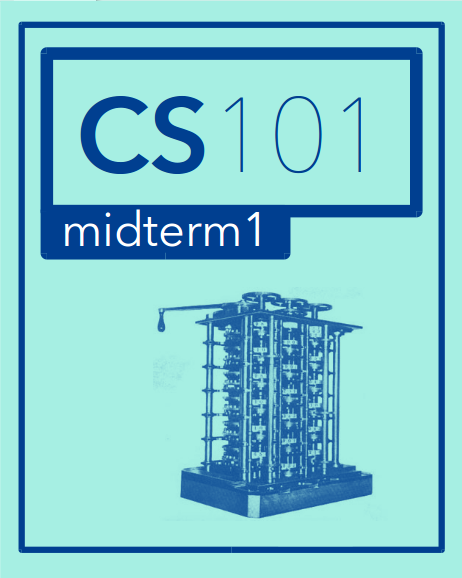
\includegraphics[width=2in]{../img/midterm1-header.png}
\end{center}

\bigskip
\noindent
\begin{itemize}
\item \textbf{Be sure to enter your \underline{NetID} and \underline{the code below} on your Scantron}.
\item Do not turn this page until instructed to do so.
\item There are 30 questions, worth 1 point each.
\item Each question has only \textbf{one} correct answer.
\item You must not communicate with other students during this test.
\item No books, notes, or electronic devices are permitted.
\item This is a 60-minute exam.
\item There are several different versions of this exam.
\end{itemize}

\bigskip\bigskip
\noindent
\textbf{\Large 1. Fill in your information:}

\bigskip
{\Large\bf
\begin{tabular}{ll}
Full Name: & \underbar{\hskip 8cm} \\[0.5em]
UIN (Student Number): & \underbar{\hskip 8cm} \\[0.5em]
NetID: & \underbar{\hskip 8cm}
\end{tabular}
}

\bigskip
\bigskip
\noindent
\textbf{\Large 2. Fill in the following answers on the Scantron form:}

%%%%%%%%%%%%%%%%%%%%%%%%%%%%%%%%%%%%%%%%%%%%%%%%%%%%%%%%%
%%%%%%%%%%%%%%%%%%%%%%%%%%%%%%%%%%%%%%%%%%%%%%%%%%%%%%%%%

\begin{enumerate}
\item[92.] C
\item[93.] C
\item[94.] A
\item[95.] C
\item[96.] D
\end{enumerate}

\newpage

% Zone 1


%%%%%%%%%%%%%%%%%%%%%%%%%%%%%%%%%%%%%%%%%%%%%%%%%%%%%%%%%



\newpage
\noindent
1. (1 point)
Consider the following program:
\begin{verbatim}
x="KING ARTHUR-MORGANA LEFAY-SIR BEDIVERE".split("-")
y=x[:]
y.reverse()
\end{verbatim}
What is the \textbf{value} of \texttt{x} after this program is executed?


\begin{enumerate}
\item[(A)]
\begin{verbatim}['BEDIVERE', 'LEFAY-SIR', 'ARTHUR-MORGANA', 'KING']\end{verbatim}

\item[(B)] $\bigstar$ 
\begin{verbatim}['KING ARTHUR', 'MORGANA LEFAY', 'SIR BEDIVERE']\end{verbatim}

\item[(C)]
\begin{verbatim}None\end{verbatim}

\item[(D)]
\begin{verbatim}['KING', 'ARTHUR-MORGANA', 'LEFAY-SIR', 'BEDIVERE']\end{verbatim}

\item[(E)]
\begin{verbatim}['SIR BEDIVERE', 'MORGANA LEFAY', 'KING ARTHUR']\end{verbatim}

\end{enumerate}

\vspace*{2em}
\hrule
\vspace{2em}

\noindent {\bf Solution.} 
\vspace{2em}
\hrule height 2pt


\newpage
\noindent
2. (1 point)
Consider the following program.
\begin{verbatim}
kay = 2
wart = 3

def knight(kay,wart):
    wart += 2
    kay += 3
    return wart + kay

wart = knight(kay, kay) + knight(wart, wart)
\end{verbatim}
After it is run, what is the final \textbf{value} of \texttt{wart}?


\begin{enumerate}
\item[(A)]
\begin{verbatim}3\end{verbatim}

\item[(B)] $\bigstar$ 
None of the other answers are correct.

\item[(C)]
\begin{verbatim}2\end{verbatim}

\item[(D)]
\begin{verbatim}5\end{verbatim}

\end{enumerate}

\vspace*{2em}
\hrule
\vspace{2em}

\noindent {\bf Solution.} 
\vspace{2em}
\hrule height 2pt


\newpage
\noindent
3. (1 point)
Evaluate the following expression:
\begin{verbatim}
len("ABCDE"[1:4])
\end{verbatim}
What value is produced?


\begin{enumerate}
\item[(A)]
1

\item[(B)] $\bigstar$ 
3

\item[(C)]
5

\item[(D)]
4

\end{enumerate}

\vspace*{2em}
\hrule
\vspace{2em}

\noindent {\bf Solution.} 
\vspace{2em}
\hrule height 2pt


\newpage
\noindent
4. (1 point)
Consider the following program:
\begin{verbatim}
x=str("1"*3)
\end{verbatim}
What is the \textbf{value} of \texttt{x} after this program is executed?


\begin{enumerate}
\item[(A)]
\begin{verbatim}"3"\end{verbatim}

\item[(B)]
\begin{verbatim}3\end{verbatim}

\item[(C)] $\bigstar$ 
\begin{verbatim}"111"\end{verbatim}

\item[(D)]
None of the other answers are correct.

\item[(E)]
\begin{verbatim}111\end{verbatim}

\end{enumerate}

\vspace*{2em}
\hrule
\vspace{2em}

\noindent {\bf Solution.} 
\vspace{2em}
\hrule height 2pt


\newpage
\noindent
5. (1 point)
What is the result of the following expression?
\begin{verbatim}
[ 1, 2, 3 ] * 3.0
\end{verbatim}


\begin{enumerate}
\item[(A)]
\begin{verbatim}None of the above.\end{verbatim}

\item[(B)]
\begin{verbatim}[3.0, 6.0, 9.0]\end{verbatim}

\item[(C)]
\begin{verbatim}[1.0, 2.0, 3.0, 1.0, 2.0, 3.0, 1.0, 2.0, 3.0]\end{verbatim}

\item[(D)] $\bigstar$ 
\begin{verbatim}[1, 2, 3, 1, 2, 3, 1, 2, 3]\end{verbatim}

\item[(E)]
\begin{verbatim}[3, 6, 9]\end{verbatim}

\end{enumerate}

\vspace*{2em}
\hrule
\vspace{2em}

\noindent {\bf Solution.} 
\vspace{2em}
\hrule height 2pt


\newpage
\noindent
6. (1 point)
Consider the following program:
\begin{verbatim}
a=["merlin","sir agravaine","king pellinore"]
b=[ ]
for i in range(0,3):
    b.append(a[0-i].title())
\end{verbatim}
What is the \textbf{value} of b after this program is executed?


\begin{enumerate}
\item[(A)]
\begin{verbatim}['Sir Agravaine', 'King Pellinore']\end{verbatim}

\item[(B)]
\begin{verbatim}['King Pellinore', 'Sir Agravaine']\end{verbatim}

\item[(C)]
\begin{verbatim}[ ]\end{verbatim}

\item[(D)]
\begin{verbatim}['King Pellinore', 'Sir Agravaine', 'Merlin']\end{verbatim}

\item[(E)] $\bigstar$ 
\begin{verbatim}['Merlin', 'King Pellinore', 'Sir Agravaine']\end{verbatim}

\end{enumerate}

\vspace*{2em}
\hrule
\vspace{2em}

\noindent {\bf Solution.} 
\vspace{2em}
\hrule height 2pt


\newpage
\noindent
7. (1 point)
Consider the following program:
\begin{verbatim}
x=0
for i in range(2,7):
    if i%3==0:
        x+=3
    elif i%2==0:
        x+=2
    else:
        x+=1
\end{verbatim}
What is the \textbf{value} of \texttt{x} after this program is executed?


\begin{enumerate}
\item[(A)] $\bigstar$ 
\begin{verbatim}11\end{verbatim}

\item[(B)]
\begin{verbatim}10\end{verbatim}

\item[(C)]
\begin{verbatim}12\end{verbatim}

\item[(D)]
\begin{verbatim}14\end{verbatim}

\item[(E)]
\begin{verbatim}13\end{verbatim}

\end{enumerate}

\vspace*{2em}
\hrule
\vspace{2em}

\noindent {\bf Solution.} 
\vspace{2em}
\hrule height 2pt


\newpage
\noindent
8. (1 point)
Consider the following program:
\begin{verbatim}
i=3
x=2
while i < 7:
    x+=i
    i+=2
\end{verbatim}
What is the \textbf{value} of \texttt{x} after this program is executed?


\begin{enumerate}
\item[(A)] $\bigstar$ 
\begin{verbatim}10\end{verbatim}

\item[(B)]
\begin{verbatim}13\end{verbatim}

\item[(C)]
\begin{verbatim}14\end{verbatim}

\item[(D)]
\begin{verbatim}11\end{verbatim}

\item[(E)]
\begin{verbatim}12\end{verbatim}

\end{enumerate}

\vspace*{2em}
\hrule
\vspace{2em}

\noindent {\bf Solution.} 
\vspace{2em}
\hrule height 2pt


\newpage
\noindent
9. (1 point)
Consider the following program:
\begin{verbatim}
x=2
a=6
if (a%3)==2:
    x=x**3
elif(a%3)==1:
    x=x**2
else:
    x=x**1
\end{verbatim}
What is the \textbf{value} of \texttt{x} after this program is executed?


\begin{enumerate}
\item[(A)]
\begin{verbatim}4\end{verbatim}

\item[(B)]
None of the other answers are correct.

\item[(C)] $\bigstar$ 
\begin{verbatim}2\end{verbatim}

\item[(D)]
\begin{verbatim}8\end{verbatim}

\item[(E)]
\begin{verbatim}16\end{verbatim}

\end{enumerate}

\vspace*{2em}
\hrule
\vspace{2em}

\noindent {\bf Solution.} 
\vspace{2em}
\hrule height 2pt


\newpage
\noindent
10. (1 point)
Consider the following incomplete function.
\begin{verbatim}
def isdivisible(m,n):
    if ???:
        return False
    else:
        return True
\end{verbatim}
The function is intended to return True if the input parameter m is evenly divisible by the parameter n and False otherwise. For example, \verb|isdivisible(4,2)| should return \verb|True|, but \verb|isdivisible(5,3)| should return \verb|False|. What should replace the three question marks to complete the function?


\begin{enumerate}
\item[(A)]
\begin{verbatim}(n % m) == 0 \end{verbatim}

\item[(B)]
\begin{verbatim}(m // n) != 0 \end{verbatim}

\item[(C)]
\begin{verbatim}(n // m) == 0 \end{verbatim}

\item[(D)] $\bigstar$ 
\begin{verbatim}(m % n) != 0 \end{verbatim}

\end{enumerate}

\vspace*{2em}
\hrule
\vspace{2em}

\noindent {\bf Solution.} 
\vspace{2em}
\hrule height 2pt


\newpage
\noindent
11. (1 point)
Consider the following program:
\begin{verbatim}
s="ECTOR"
t="GAWAIN"
x=(len(s)+len(t)) < 4 and s in t
\end{verbatim}
What is the \textbf{type} of \texttt{x} after this program is executed?


\begin{enumerate}
\item[(A)]
\begin{verbatim}None\end{verbatim}

\item[(B)]
\begin{verbatim}Float\end{verbatim}

\item[(C)] $\bigstar$ 
\begin{verbatim}Boolean\end{verbatim}

\item[(D)]
\begin{verbatim}Integer\end{verbatim}

\item[(E)]
\begin{verbatim}String\end{verbatim}

\end{enumerate}

\vspace*{2em}
\hrule
\vspace{2em}

\noindent {\bf Solution.} 
\vspace{2em}
\hrule height 2pt


\newpage
\noindent
12. (1 point)
Consider the following program:
\begin{verbatim}
s="G+R+A+I+L"
x=s.split("+")[1:-2]
\end{verbatim}
What is the \textbf{value} of \texttt{x} after this program is executed?


\begin{enumerate}
\item[(A)]
\begin{verbatim}None\end{verbatim}

\item[(B)]
\begin{verbatim}'RAI'\end{verbatim}

\item[(C)] $\bigstar$ 
\begin{verbatim}['R','A']\end{verbatim}

\item[(D)]
\begin{verbatim}3\end{verbatim}

\item[(E)]
\begin{verbatim}False\end{verbatim}

\end{enumerate}

\vspace*{2em}
\hrule
\vspace{2em}

\noindent {\bf Solution.} 
\vspace{2em}
\hrule height 2pt


\newpage
\noindent
13. (1 point)
Consider the following Python program.
\begin{verbatim}
e=[1,3,5,7,9,11]
d=[0,0,0]
for i in range(0,len(e)):
    d[i%3]+=e[i]
x=d[1]
\end{verbatim}
After it is run, what is the final \textbf{value} of \texttt{x}?


\begin{enumerate}
\item[(A)]
\begin{verbatim}3\end{verbatim}

\item[(B)]
\begin{verbatim}8\end{verbatim}

\item[(C)]
\begin{verbatim}16\end{verbatim}

\item[(D)]
\begin{verbatim}0\end{verbatim}

\item[(E)] $\bigstar$ 
\begin{verbatim}12\end{verbatim}

\end{enumerate}

\vspace*{2em}
\hrule
\vspace{2em}

\noindent {\bf Solution.} 
\vspace{2em}
\hrule height 2pt


\newpage
\noindent
14. (1 point)
Consider the following program.
\begin{verbatim}
s="ABCBA"
x=0
y=len(s)-1
while s[x]==s[y] and x<y:
    x+=1
    y-=1
\end{verbatim}
After it is run, what is the final \textbf{value} of \texttt{x}?


\begin{enumerate}
\item[(A)]
\begin{verbatim}1\end{verbatim}

\item[(B)]
\begin{verbatim}0\end{verbatim}

\item[(C)]
\begin{verbatim}3\end{verbatim}

\item[(D)] $\bigstar$ 
\begin{verbatim}2\end{verbatim}

\item[(E)]
\begin{verbatim}4\end{verbatim}

\end{enumerate}

\vspace*{2em}
\hrule
\vspace{2em}

\noindent {\bf Solution.} 
\vspace{2em}
\hrule height 2pt


\newpage
\noindent
15. (1 point)
Consider the following program:
\begin{verbatim}
a=3
b=4
if a==3:
    a=b
elif a==4:
    a=5
else:
    b=a
\end{verbatim}
What is the \textbf{value} of a after this program is executed?


\begin{enumerate}
\item[(A)]
\begin{verbatim}5\end{verbatim}

\item[(B)] $\bigstar$ 
\begin{verbatim}4\end{verbatim}

\item[(C)]
None of the other answers are correct.

\item[(D)]
\begin{verbatim}7\end{verbatim}

\item[(E)]
\begin{verbatim}3\end{verbatim}

\end{enumerate}

\vspace*{2em}
\hrule
\vspace{2em}

\noindent {\bf Solution.} 
\vspace{2em}
\hrule height 2pt


\newpage
\noindent
16. (1 point)
Evaluate the following expression:
\begin{verbatim}
[1,2]+[len("3")]
\end{verbatim}
What value is produced?


\begin{enumerate}
\item[(A)]
\begin{verbatim}[1,2,1,2,1,2]\end{verbatim}

\item[(B)]
\begin{verbatim}[1,2,"3"]\end{verbatim}

\item[(C)]
\begin{verbatim}[1,2,3]\end{verbatim}

\item[(D)] $\bigstar$ 
\begin{verbatim}[1,2,1]\end{verbatim}

\end{enumerate}

\vspace*{2em}
\hrule
\vspace{2em}

\noindent {\bf Solution.} 
\vspace{2em}
\hrule height 2pt


\newpage
\noindent
17. (1 point)
Consider the following program:
\begin{verbatim}
a=["S","T","U","P","E","F","Y"]
a=a[0:4]
a.sort()
x=""
for e in a:
    x=e+x
\end{verbatim}
What is the \textbf{value} of \texttt{x} after this program is executed?


\begin{enumerate}
\item[(A)] $\bigstar$ 
\begin{verbatim}"UTSP"\end{verbatim}

\item[(B)]
None of the other answers are correct.

\item[(C)]
\begin{verbatim}"STUP"\end{verbatim}

\item[(D)]
\begin{verbatim}"PSTU"\end{verbatim}

\item[(E)]
\begin{verbatim}"PUST"\end{verbatim}

\end{enumerate}

\vspace*{2em}
\hrule
\vspace{2em}

\noindent {\bf Solution.} 
\vspace{2em}
\hrule height 2pt


\newpage
\noindent
18. (1 point)
Consider the following program:
\begin{verbatim}
x=[1,2,3,4,5,6,7,8,9]
x=x[2:-2]
i=1
while i < 3:
    x[i]+=1
    i+=1
\end{verbatim}
What is the \textbf{value} of \texttt{x} after this program is executed?


\begin{enumerate}
\item[(A)]
\begin{verbatim}[3, 5, 6, 6, 7, 8]\end{verbatim}

\item[(B)] $\bigstar$ 
\begin{verbatim}[3, 5, 6, 6, 7]\end{verbatim}

\item[(C)]
\begin{verbatim}[2, 4, 5, 5, 6, 7]\end{verbatim}

\item[(D)]
\begin{verbatim}[2, 4, 5, 6, 6, 7]\end{verbatim}

\item[(E)]
\begin{verbatim}[3, 5, 6, 6]\end{verbatim}

\end{enumerate}

\vspace*{2em}
\hrule
\vspace{2em}

\noindent {\bf Solution.} 
\vspace{2em}
\hrule height 2pt


\newpage
\noindent
19. (1 point)
Consider the following program:
\begin{verbatim}
def fix(s):
    a=list(s)
    a.sort()
    return ''.join(a)

x=["one","two","eleven","twelve"]
s1=fix(x[0]+x[-1])
s2=fix(x[1]+x[-2])

if s1<s2:
    x.sort()
elif s1>s2:
    x.reverse()
else:
    x.append("six")
\end{verbatim}
What is the \textbf{value} of \texttt{x} after this program is executed?


\begin{enumerate}
\item[(A)]
\begin{verbatim}['twelve', 'eleven', 'two', 'one']\end{verbatim}

\item[(B)]
\begin{verbatim}['one', 'two', 'eleven', 'twelve']\end{verbatim}

\item[(C)] $\bigstar$ 
\begin{verbatim}['one', 'two', 'eleven', 'twelve', 'six']\end{verbatim}

\item[(D)]
\begin{verbatim}['two', 'twelve', 'one', 'eleven', 'six']\end{verbatim}

\item[(E)]
\begin{verbatim}['eleven', 'one', 'twelve', 'two']\end{verbatim}

\end{enumerate}

\vspace*{2em}
\hrule
\vspace{2em}

\noindent {\bf Solution.} 
\vspace{2em}
\hrule height 2pt


\newpage
\noindent
20. (1 point)
Consider the following incomplete Python program.
\begin{verbatim}
s="".join(["2","2","0","1"])
x=0
for i in range(len(s)-1):
    x+=int(???)
\end{verbatim}
What should replace the three question marks so the resulting value of \texttt{x} is 43?


\begin{enumerate}
\item[(A)]
\begin{verbatim}s[i+1:i+2]\end{verbatim}

\item[(B)]
\begin{verbatim}s[i:i+1]\end{verbatim}

\item[(C)]
\begin{verbatim}s[i:i-1]\end{verbatim}

\item[(D)] $\bigstar$ 
\begin{verbatim}s[i:i+2]\end{verbatim}

\end{enumerate}

\vspace*{2em}
\hrule
\vspace{2em}

\noindent {\bf Solution.} 
\vspace{2em}
\hrule height 2pt


\newpage
\noindent
21. (1 point)
Consider the following program.
\begin{verbatim}
x=0
i=1
while(i*i)<=9:
    x=x+(i*i)
    i=i+1
\end{verbatim}
After it is run, what is the final \textbf{value} of \texttt{x}?


\begin{enumerate}
\item[(A)]
\begin{verbatim}5\end{verbatim}

\item[(B)]
\begin{verbatim}30\end{verbatim}

\item[(C)] $\bigstar$ 
\begin{verbatim}14\end{verbatim}

\item[(D)]
\begin{verbatim}4\end{verbatim}

\item[(E)]
\begin{verbatim}3\end{verbatim}

\end{enumerate}

\vspace*{2em}
\hrule
\vspace{2em}

\noindent {\bf Solution.} 
\vspace{2em}
\hrule height 2pt


\newpage
\noindent
22. (1 point)
For this problem, you should compose a function which accomplishes a given task using the available code blocks arranged in the correct functional order.  \emph{We ignore indentation for this problem.}

\texttt{find\_max} should accept a \texttt{list} and return the value of the maximum item in the \texttt{list}.  (\texttt{None} is always the lowest value in any numeric comparison, so you may use it as an initializer.)

\begin{verbatim}
def find_max(my_list):
\end{verbatim}

\begin{enumerate}[1]
\item \texttt{max\_val = i}
\item \texttt{max\_val = None}
\item \texttt{for i in range(len(my\_list)):}
\item \texttt{if i > max\_val:}
\item \texttt{max\_val = my\_list[i]}
\item \texttt{return max\_val}
\item \texttt{for i in range(my\_list):}
\item \texttt{if my\_list[i] > max\_val:}
\item \texttt{print(max\_val)}
\end{enumerate}



\begin{enumerate}
\item[(A)]
2, 7, 4, 5, 6

\item[(B)] $\bigstar$ 
2, 3, 8, 5, 6

\item[(C)]
3, 2, 8, 5, 9

\item[(D)]
2, 3, 4, 1, 6

\item[(E)]
2, 3, 8, 1, 6

\end{enumerate}

\vspace*{2em}
\hrule
\vspace{2em}

\noindent {\bf Solution.} 
\vspace{2em}
\hrule height 2pt


\newpage
\noindent
23. (1 point)
Consider the following program:
\begin{verbatim}
s="Hobbes"
i=0
x=-1
while i<len(s):
    if s[i]=='b':
        x=i
    i+=1
\end{verbatim}
What is the \textbf{value} of \texttt{x} after this program is executed?


\begin{enumerate}
\item[(A)]
\begin{verbatim}2\end{verbatim}

\item[(B)] $\bigstar$ 
\begin{verbatim}3\end{verbatim}

\item[(C)]
\begin{verbatim}5\end{verbatim}

\item[(D)]
\begin{verbatim}4\end{verbatim}

\item[(E)]
\begin{verbatim}-1\end{verbatim}

\end{enumerate}

\vspace*{2em}
\hrule
\vspace{2em}

\noindent {\bf Solution.} 
\vspace{2em}
\hrule height 2pt


\newpage
\noindent
24. (1 point)
Consider the following program.
\begin{verbatim}
def artificing(s):
    return s*2
    return s+"%i" % 2
    return s

s=artificing("MERLIN")
\end{verbatim}
After it is run, what is the final \textbf{value} of s?


\begin{enumerate}
\item[(A)] $\bigstar$ 
\begin{verbatim}"MERLINMERLIN"\end{verbatim}

\item[(B)]
\begin{verbatim}None\end{verbatim}

\item[(C)]
\begin{verbatim}12\end{verbatim}

\item[(D)]
\begin{verbatim}"MERLIN2"\end{verbatim}

\item[(E)]
\begin{verbatim}"MERLIN"\end{verbatim}

\end{enumerate}

\vspace*{2em}
\hrule
\vspace{2em}

\noindent {\bf Solution.} 
\vspace{2em}
\hrule height 2pt


\newpage
\noindent
25. (1 point)
Consider the following program:
\begin{verbatim}
pi="3.14159"
e="2.71828"
x=pi*len(e)+pi
\end{verbatim}
What is the \textbf{type} of \texttt{x} after this program is executed?


\begin{enumerate}
\item[(A)]
\begin{verbatim}None\end{verbatim}

\item[(B)]
\begin{verbatim}Integer\end{verbatim}

\item[(C)]
\begin{verbatim}Float\end{verbatim}

\item[(D)]
\begin{verbatim}Boolean\end{verbatim}

\item[(E)] $\bigstar$ 
\begin{verbatim}String\end{verbatim}

\end{enumerate}

\vspace*{2em}
\hrule
\vspace{2em}

\noindent {\bf Solution.} 
\vspace{2em}
\hrule height 2pt


\newpage
\noindent
26. (1 point)
Consider the following program.
\begin{verbatim}
x=[]
for j in range(0,5):
    if (j%2)==0:
        x.append("-")
    if (j%5)==0:
        x.append("*")
\end{verbatim}
After it is run, what is the final \textbf{value} of \texttt{x}?


\begin{enumerate}
\item[(A)]
None of the other answers are correct.

\item[(B)] $\bigstar$ 
\begin{verbatim}["-","*","-","-"]\end{verbatim}

\item[(C)]
\begin{verbatim}["*","-","*","*"]\end{verbatim}

\item[(D)]
\begin{verbatim}["-","-","*"]\end{verbatim}

\item[(E)]
\begin{verbatim}["-","*","-"]\end{verbatim}

\end{enumerate}

\vspace*{2em}
\hrule
\vspace{2em}

\noindent {\bf Solution.} 
\vspace{2em}
\hrule height 2pt


\newpage
\noindent
27. (1 point)
Consider the following incomplete program.
\begin{verbatim}
sum=0
???:
    sum=sum+i

\end{verbatim}
The program is intended to sum all of the integers between 1 and 100 (inclusive). What should replace the three question marks to complete the program?


\begin{enumerate}
\item[(A)] $\bigstar$ 
\begin{verbatim}for i in range(1,101) \end{verbatim}

\item[(B)]
\begin{verbatim}while i in range(100)\end{verbatim}

\item[(C)]
\begin{verbatim}for i in range(0,100)\end{verbatim}

\item[(D)]
\begin{verbatim}while i<=100 \end{verbatim}

\end{enumerate}

\vspace*{2em}
\hrule
\vspace{2em}

\noindent {\bf Solution.} 
\vspace{2em}
\hrule height 2pt


\newpage
\noindent
28. (1 point)
Consider the following program:
\begin{verbatim}
x=[1,2,3]
def f(a):
    s=""
    a.reverse()
    for i in a:
        s+=str(i)
    return s

x.append(f(x))
\end{verbatim}
What is the \textbf{value} of \texttt{x} after this program is executed?


\begin{enumerate}
\item[(A)]
\begin{verbatim}[1, 2, 3, 6]\end{verbatim}

\item[(B)]
\begin{verbatim}[1, 2, 3]\end{verbatim}

\item[(C)]
\begin{verbatim}[3, 2, 1]\end{verbatim}

\item[(D)] $\bigstar$ 
\begin{verbatim}[3, 2, 1, '321']\end{verbatim}

\item[(E)]
\begin{verbatim}[1, 2, 3, '321']\end{verbatim}

\end{enumerate}

\vspace*{2em}
\hrule
\vspace{2em}

\noindent {\bf Solution.} 
\vspace{2em}
\hrule height 2pt


\newpage
\noindent
29. (1 point)
Consider the following program:
\begin{verbatim}
s="TRIS %i"
t="ISEU"
x=len(s) % len(t[2:-1])
\end{verbatim}
What is the \textbf{type} of \texttt{x} after this program is executed?


\begin{enumerate}
\item[(A)]
\begin{verbatim}String\end{verbatim}

\item[(B)]
\begin{verbatim}None\end{verbatim}

\item[(C)]
\begin{verbatim}Boolean\end{verbatim}

\item[(D)] $\bigstar$ 
\begin{verbatim}Integer\end{verbatim}

\item[(E)]
\begin{verbatim}Float\end{verbatim}

\end{enumerate}

\vspace*{2em}
\hrule
\vspace{2em}

\noindent {\bf Solution.} 
\vspace{2em}
\hrule height 2pt


\newpage
\noindent
30. (1 point)
How can the following mathematical equation be implemented as a Python expression? Assume \verb|a|, \verb|b|, and \verb|sin| have already been defined.
$$a \sin(a^b - b)$$


\begin{enumerate}
\item[(A)] $\bigstar$ 
\begin{verbatim}a*sin(a**b - b)\end{verbatim}

\item[(B)]
None of the other answers are correct.

\item[(C)]
\begin{verbatim}a*sin(a^b - b)\end{verbatim}

\item[(D)]
\begin{verbatim}a sin(a**b - b)\end{verbatim}

\item[(E)]
\begin{verbatim}a*sin(b^a - b)\end{verbatim}

\end{enumerate}

\vspace*{2em}
\hrule
\vspace{2em}

\noindent {\bf Solution.} 
\vspace{2em}
\hrule height 2pt

%%%%%%%%%%%%%%%%%%%%%%%%%%%%%%%%%%%%%%%%%%%%%%%%%%%%%%%%%%%%%%%%%%%%%%
%%%%%%%%%%%%%%%%%%%%%%%%%%%%%%%%%%%%%%%%%%%%%%%%%%%%%%%%%%%%%%%%%%%%%%
%%%%%%%%%%%%%%%%%%%%%%%%%%%%%%%%%%%%%%%%%%%%%%%%%%%%%%%%%%%%%%%%%%%%%%
%%%%%%%%%%%%%%%%%%%%%%%%%%%%%%%%%%%%%%%%%%%%%%%%%%%%%%%%%%%%%%%%%%%%%%
% Exam number 14

\message{Exam 14/50}
\cleardoublepage
\setcounter{page}{1}


\begin{center}
%\textbf{\Large CS 101 Midterm \#1}
%
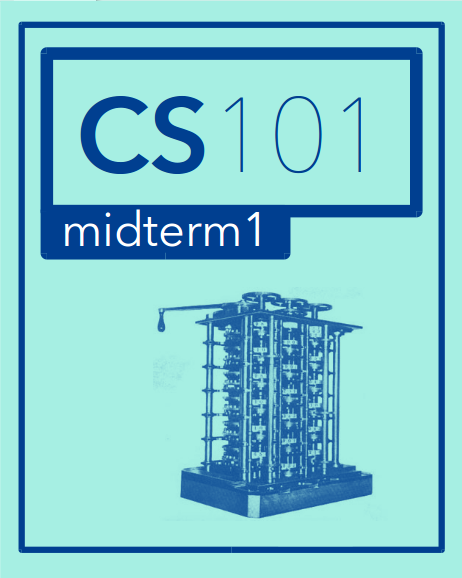
\includegraphics[width=2in]{../img/midterm1-header.png}
\end{center}

\bigskip
\noindent
\begin{itemize}
\item \textbf{Be sure to enter your \underline{NetID} and \underline{the code below} on your Scantron}.
\item Do not turn this page until instructed to do so.
\item There are 30 questions, worth 1 point each.
\item Each question has only \textbf{one} correct answer.
\item You must not communicate with other students during this test.
\item No books, notes, or electronic devices are permitted.
\item This is a 60-minute exam.
\item There are several different versions of this exam.
\end{itemize}

\bigskip\bigskip
\noindent
\textbf{\Large 1. Fill in your information:}

\bigskip
{\Large\bf
\begin{tabular}{ll}
Full Name: & \underbar{\hskip 8cm} \\[0.5em]
UIN (Student Number): & \underbar{\hskip 8cm} \\[0.5em]
NetID: & \underbar{\hskip 8cm}
\end{tabular}
}

\bigskip
\bigskip
\noindent
\textbf{\Large 2. Fill in the following answers on the Scantron form:}

%%%%%%%%%%%%%%%%%%%%%%%%%%%%%%%%%%%%%%%%%%%%%%%%%%%%%%%%%
%%%%%%%%%%%%%%%%%%%%%%%%%%%%%%%%%%%%%%%%%%%%%%%%%%%%%%%%%

\begin{enumerate}
\item[92.] D
\item[93.] C
\item[94.] A
\item[95.] D
\item[96.] E
\end{enumerate}

\newpage

% Zone 1


%%%%%%%%%%%%%%%%%%%%%%%%%%%%%%%%%%%%%%%%%%%%%%%%%%%%%%%%%



\newpage
\noindent
1. (1 point)
\begin{verbatim}
x=str(3)+"str(3)"
\end{verbatim}
What is the \textbf{value} of \texttt{x} after this program is executed?


\begin{enumerate}
\item[(A)]
\begin{verbatim}"33"\end{verbatim}

\item[(B)] $\bigstar$ 
\begin{verbatim}"3str(3)"\end{verbatim}

\item[(C)]
None of the other answers are correct.

\item[(D)]
\begin{verbatim}"333"\end{verbatim}

\item[(E)]
\begin{verbatim}33\end{verbatim}

\end{enumerate}

\vspace*{2em}
\hrule
\vspace{2em}

\noindent {\bf Solution.} 
\vspace{2em}
\hrule height 2pt


\newpage
\noindent
2. (1 point)
Consider the following incomplete program.
\begin{verbatim}
sum=0
???:
    sum=sum+i

\end{verbatim}
The program is intended to sum all of the integers between 1 and 100 (inclusive). What should replace the three question marks to complete the program?


\begin{enumerate}
\item[(A)]
\begin{verbatim}for i in range(0,100)\end{verbatim}

\item[(B)]
\begin{verbatim}while i in range(100)\end{verbatim}

\item[(C)]
\begin{verbatim}while i<=100 \end{verbatim}

\item[(D)] $\bigstar$ 
\begin{verbatim}for i in range(1,101) \end{verbatim}

\end{enumerate}

\vspace*{2em}
\hrule
\vspace{2em}

\noindent {\bf Solution.} 
\vspace{2em}
\hrule height 2pt


\newpage
\noindent
3. (1 point)
Consider the following program:
\begin{verbatim}
def fix(s):
    a=list(s)
    a.sort()
    return ''.join(a)

x=["one","two","eleven","twelve"]
s1=fix(x[0]+x[-1])
s2=fix(x[1]+x[-2])

if s1<s2:
    x.sort()
elif s1>s2:
    x.reverse()
else:
    x.append("six")
\end{verbatim}
What is the \textbf{value} of \texttt{x} after this program is executed?


\begin{enumerate}
\item[(A)] $\bigstar$ 
\begin{verbatim}['one', 'two', 'eleven', 'twelve', 'six']\end{verbatim}

\item[(B)]
\begin{verbatim}['eleven', 'one', 'twelve', 'two']\end{verbatim}

\item[(C)]
\begin{verbatim}['one', 'two', 'eleven', 'twelve']\end{verbatim}

\item[(D)]
\begin{verbatim}['twelve', 'eleven', 'two', 'one']\end{verbatim}

\item[(E)]
\begin{verbatim}['two', 'twelve', 'one', 'eleven', 'six']\end{verbatim}

\end{enumerate}

\vspace*{2em}
\hrule
\vspace{2em}

\noindent {\bf Solution.} 
\vspace{2em}
\hrule height 2pt


\newpage
\noindent
4. (1 point)
Consider the following Python program.
\begin{verbatim}
e=[1,3,5,7,9,11]
d=[0,0,0]
for i in range(0,len(e)):
    d[i%3]+=e[i]
x=d[1]
\end{verbatim}
After it is run, what is the final \textbf{value} of \texttt{x}?


\begin{enumerate}
\item[(A)]
\begin{verbatim}0\end{verbatim}

\item[(B)]
\begin{verbatim}16\end{verbatim}

\item[(C)]
\begin{verbatim}8\end{verbatim}

\item[(D)]
\begin{verbatim}3\end{verbatim}

\item[(E)] $\bigstar$ 
\begin{verbatim}12\end{verbatim}

\end{enumerate}

\vspace*{2em}
\hrule
\vspace{2em}

\noindent {\bf Solution.} 
\vspace{2em}
\hrule height 2pt


\newpage
\noindent
5. (1 point)
Consider the following program.
\begin{verbatim}
kay = 2
wart = 3

def knight(kay,wart):
    wart += 2
    kay += 3
    return wart + kay

kay = knight(wart, kay) + knight(kay, wart)
\end{verbatim}
After it is run, what is the final \textbf{value} of \texttt{kay}?


\begin{enumerate}
\item[(A)]
\begin{verbatim}2\end{verbatim}

\item[(B)] $\bigstar$ 
None of the other answers are correct.

\item[(C)]
\begin{verbatim}3\end{verbatim}

\item[(D)]
\begin{verbatim}5\end{verbatim}

\end{enumerate}

\vspace*{2em}
\hrule
\vspace{2em}

\noindent {\bf Solution.} 
\vspace{2em}
\hrule height 2pt


\newpage
\noindent
6. (1 point)
Consider the following incomplete Python program.
\begin{verbatim}
s="".join(["0","1","2","1"])
x=0
for i in range(len(s)-1):
    x+=int(???)
\end{verbatim}
What should replace the three question marks so the resulting value of \texttt{x} is 34?


\begin{enumerate}
\item[(A)]
\begin{verbatim}s[i+1:i+2]\end{verbatim}

\item[(B)]
\begin{verbatim}s[i:i+1]\end{verbatim}

\item[(C)]
\begin{verbatim}s[i:i-1]\end{verbatim}

\item[(D)] $\bigstar$ 
\begin{verbatim}s[i:i+2]\end{verbatim}

\end{enumerate}

\vspace*{2em}
\hrule
\vspace{2em}

\noindent {\bf Solution.} 
\vspace{2em}
\hrule height 2pt


\newpage
\noindent
7. (1 point)
Consider the following program:
\begin{verbatim}
a=3
b=4
if a==3:
    b=a
elif a==4:
    a=5
else:
    a=b
\end{verbatim}
What is the \textbf{value} of a after this program is executed?


\begin{enumerate}
\item[(A)] $\bigstar$ 
\begin{verbatim}3\end{verbatim}

\item[(B)]
\begin{verbatim}4\end{verbatim}

\item[(C)]
None of the other answers are correct.

\item[(D)]
\begin{verbatim}5\end{verbatim}

\item[(E)]
\begin{verbatim}7\end{verbatim}

\end{enumerate}

\vspace*{2em}
\hrule
\vspace{2em}

\noindent {\bf Solution.} 
\vspace{2em}
\hrule height 2pt


\newpage
\noindent
8. (1 point)
Consider the following program:
\begin{verbatim}
a=["merlin","sir agravaine","king pellinore"]
b=[ ]
for i in range(1,3):
    b.append(a[0-i].title())
\end{verbatim}
What is the \textbf{value} of b after this program is executed?


\begin{enumerate}
\item[(A)]
\begin{verbatim}['King Pellinore', 'Sir Agravaine', 'Merlin']\end{verbatim}

\item[(B)]
\begin{verbatim}['Merlin', 'King Pellinore', 'Sir Agravaine']\end{verbatim}

\item[(C)] $\bigstar$ 
\begin{verbatim}['King Pellinore', 'Sir Agravaine']\end{verbatim}

\item[(D)]
\begin{verbatim}[ ]\end{verbatim}

\item[(E)]
\begin{verbatim}['Sir Agravaine', 'King Pellinore']\end{verbatim}

\end{enumerate}

\vspace*{2em}
\hrule
\vspace{2em}

\noindent {\bf Solution.} 
\vspace{2em}
\hrule height 2pt


\newpage
\noindent
9. (1 point)
Consider the following program:
\begin{verbatim}
x=3
a=5
if (a%3)==2:
    x=x**3
elif(a%3)==1:
    x=x**2
else:
    x=x**1
\end{verbatim}
What is the \textbf{value} of \texttt{x} after this program is executed?


\begin{enumerate}
\item[(A)]
\begin{verbatim}1\end{verbatim}

\item[(B)]
\begin{verbatim}3\end{verbatim}

\item[(C)]
None of the other answers are correct.

\item[(D)]
\begin{verbatim}9\end{verbatim}

\item[(E)] $\bigstar$ 
\begin{verbatim}27\end{verbatim}

\end{enumerate}

\vspace*{2em}
\hrule
\vspace{2em}

\noindent {\bf Solution.} 
\vspace{2em}
\hrule height 2pt


\newpage
\noindent
10. (1 point)
Consider the following program.
\begin{verbatim}
x=1
i=0
while(x*x)<=9:
    i=i+(x*x)
    x=x+1
\end{verbatim}
After it is run, what is the final \textbf{value} of \texttt{x}?


\begin{enumerate}
\item[(A)]
\begin{verbatim}5\end{verbatim}

\item[(B)]
\begin{verbatim}3\end{verbatim}

\item[(C)]
\begin{verbatim}30\end{verbatim}

\item[(D)]
\begin{verbatim}14\end{verbatim}

\item[(E)] $\bigstar$ 
\begin{verbatim}4\end{verbatim}

\end{enumerate}

\vspace*{2em}
\hrule
\vspace{2em}

\noindent {\bf Solution.} 
\vspace{2em}
\hrule height 2pt


\newpage
\noindent
11. (1 point)
Consider the following program.
\begin{verbatim}
def artificing(s):
    return s+"%i" % 2
    return s*2
    return s

s=artificing("MERLIN")
\end{verbatim}
After it is run, what is the final \textbf{value} of s?


\begin{enumerate}
\item[(A)]
\begin{verbatim}"MERLIN%i"\end{verbatim}

\item[(B)]
\begin{verbatim}None\end{verbatim}

\item[(C)]
\begin{verbatim}0\end{verbatim}

\item[(D)]
\begin{verbatim}"MERLINMERLIN"\end{verbatim}

\item[(E)] $\bigstar$ 
\begin{verbatim}"MERLIN2"\end{verbatim}

\end{enumerate}

\vspace*{2em}
\hrule
\vspace{2em}

\noindent {\bf Solution.} 
\vspace{2em}
\hrule height 2pt


\newpage
\noindent
12. (1 point)
Evaluate the following expression:
\begin{verbatim}
[1,2]*len("3")
\end{verbatim}
What value is produced?


\begin{enumerate}
\item[(A)] $\bigstar$ 
\begin{verbatim}[1,2]\end{verbatim}

\item[(B)]
\begin{verbatim}[1,2,3]\end{verbatim}

\item[(C)]
\begin{verbatim}[1,2,1]\end{verbatim}

\item[(D)]
\begin{verbatim}[1,2,1,2,1,2]\end{verbatim}

\end{enumerate}

\vspace*{2em}
\hrule
\vspace{2em}

\noindent {\bf Solution.} 
\vspace{2em}
\hrule height 2pt


\newpage
\noindent
13. (1 point)
Consider the following program.
\begin{verbatim}
x=[]
for j in range(0,5):
    if (j%3)==0:
        x.append("-")
    if (j%4)==0:
        x.append("*")
\end{verbatim}
After it is run, what is the final \textbf{value} of \texttt{x}?


\begin{enumerate}
\item[(A)]
\begin{verbatim}["*","-","*"]\end{verbatim}

\item[(B)]
\begin{verbatim}["*","-","*"]\end{verbatim}

\item[(C)]
\begin{verbatim}["-","*"]\end{verbatim}

\item[(D)] $\bigstar$ 
\begin{verbatim}["-","*","-","*"]\end{verbatim}

\item[(E)]
None of the other answers are correct.

\end{enumerate}

\vspace*{2em}
\hrule
\vspace{2em}

\noindent {\bf Solution.} 
\vspace{2em}
\hrule height 2pt


\newpage
\noindent
14. (1 point)
Consider the following program:
\begin{verbatim}
pi="3.14159"
e="2.71828"
x=pi*len(e)+pi
\end{verbatim}
What is the \textbf{type} of \texttt{x} after this program is executed?


\begin{enumerate}
\item[(A)]
\begin{verbatim}None\end{verbatim}

\item[(B)]
\begin{verbatim}Boolean\end{verbatim}

\item[(C)] $\bigstar$ 
\begin{verbatim}String\end{verbatim}

\item[(D)]
\begin{verbatim}Integer\end{verbatim}

\item[(E)]
\begin{verbatim}Float\end{verbatim}

\end{enumerate}

\vspace*{2em}
\hrule
\vspace{2em}

\noindent {\bf Solution.} 
\vspace{2em}
\hrule height 2pt


\newpage
\noindent
15. (1 point)
Consider the following program.
\begin{verbatim}
s="BBCAA"
x=0
y=len(s)-1
while s[x]!=s[y] and x<len(s):
    x+=1
    y-=1
\end{verbatim}
After it is run, what is the final \textbf{value} of \texttt{x}?


\begin{enumerate}
\item[(A)]
\begin{verbatim}3\end{verbatim}

\item[(B)]
\begin{verbatim}0\end{verbatim}

\item[(C)]
\begin{verbatim}4\end{verbatim}

\item[(D)]
\begin{verbatim}1\end{verbatim}

\item[(E)] $\bigstar$ 
\begin{verbatim}2\end{verbatim}

\end{enumerate}

\vspace*{2em}
\hrule
\vspace{2em}

\noindent {\bf Solution.} 
\vspace{2em}
\hrule height 2pt


\newpage
\noindent
16. (1 point)
Consider the following program:
\begin{verbatim}
s="ECTOR"
t="GAWAIN"
x=(len(s)+len(t)) < 4 and s in t
\end{verbatim}
What is the \textbf{type} of \texttt{x} after this program is executed?


\begin{enumerate}
\item[(A)]
\begin{verbatim}String\end{verbatim}

\item[(B)]
\begin{verbatim}None\end{verbatim}

\item[(C)] $\bigstar$ 
\begin{verbatim}Boolean\end{verbatim}

\item[(D)]
\begin{verbatim}Integer\end{verbatim}

\item[(E)]
\begin{verbatim}Float\end{verbatim}

\end{enumerate}

\vspace*{2em}
\hrule
\vspace{2em}

\noindent {\bf Solution.} 
\vspace{2em}
\hrule height 2pt


\newpage
\noindent
17. (1 point)
Consider the following program:
\begin{verbatim}
x=0
for i in range(2,8):
    if i%3==0:
        x+=3
    elif i%2==0:
        x+=2
    else:
        x+=1
\end{verbatim}
What is the \textbf{value} of \texttt{x} after this program is executed?


\begin{enumerate}
\item[(A)]
\begin{verbatim}11\end{verbatim}

\item[(B)]
\begin{verbatim}10\end{verbatim}

\item[(C)] $\bigstar$ 
\begin{verbatim}12\end{verbatim}

\item[(D)]
\begin{verbatim}14\end{verbatim}

\item[(E)]
\begin{verbatim}13\end{verbatim}

\end{enumerate}

\vspace*{2em}
\hrule
\vspace{2em}

\noindent {\bf Solution.} 
\vspace{2em}
\hrule height 2pt


\newpage
\noindent
18. (1 point)
Consider the following program:
\begin{verbatim}
x="KING ARTHUR-MORGANA LEFAY-SIR BEDIVERE".split("-")
y=x
y.reverse()
\end{verbatim}
What is the \textbf{value} of \texttt{x} after this program is executed?


\begin{enumerate}
\item[(A)]
\begin{verbatim}['KING ARTHUR', 'MORGANA LEFAY', 'SIR BEDIVERE']\end{verbatim}

\item[(B)] $\bigstar$ 
\begin{verbatim}['SIR BEDIVERE', 'MORGANA LEFAY', 'KING ARTHUR']\end{verbatim}

\item[(C)]
\begin{verbatim}['KING', 'ARTHUR-MORGANA', 'LEFAY-SIR', 'BEDIVERE']\end{verbatim}

\item[(D)]
\begin{verbatim}None\end{verbatim}

\item[(E)]
\begin{verbatim}['BEDIVERE', 'LEFAY-SIR', 'ARTHUR-MORGANA', 'KING']\end{verbatim}

\end{enumerate}

\vspace*{2em}
\hrule
\vspace{2em}

\noindent {\bf Solution.} 
\vspace{2em}
\hrule height 2pt


\newpage
\noindent
19. (1 point)
Consider the following program:
\begin{verbatim}
s="-B-O-R-S-"
x=s.split("-")[2:-2]
\end{verbatim}
What is the \textbf{value} of \texttt{x} after this program is executed?


\begin{enumerate}
\item[(A)]
\begin{verbatim}False\end{verbatim}

\item[(B)]
\begin{verbatim}''\end{verbatim}

\item[(C)]
\begin{verbatim}'ORS'\end{verbatim}

\item[(D)]
\begin{verbatim}None\end{verbatim}

\item[(E)] $\bigstar$ 
\begin{verbatim}['O', 'R']\end{verbatim}

\end{enumerate}

\vspace*{2em}
\hrule
\vspace{2em}

\noindent {\bf Solution.} 
\vspace{2em}
\hrule height 2pt


\newpage
\noindent
20. (1 point)
For this problem, you should compose a function which accomplishes a given task using the available code blocks arranged in the correct functional order.  \emph{We ignore indentation for this problem.}

\texttt{find\_max} should accept a \texttt{list} and return the value of the maximum item in the \texttt{list}.  (\texttt{None} is always the lowest value in any numeric comparison, so you may use it as an initializer.)

\begin{verbatim}
def find_max(my_list):
\end{verbatim}

\begin{enumerate}[1]
\item \texttt{max\_val = i}
\item \texttt{max\_val = None}
\item \texttt{for i in range(len(my\_list)):}
\item \texttt{if i > max\_val:}
\item \texttt{max\_val = my\_list[i]}
\item \texttt{return max\_val}
\item \texttt{for i in range(my\_list):}
\item \texttt{if my\_list[i] > max\_val:}
\item \texttt{print(max\_val)}
\end{enumerate}



\begin{enumerate}
\item[(A)]
2, 3, 8, 1, 6

\item[(B)]
2, 3, 4, 1, 6

\item[(C)]
2, 7, 4, 5, 6

\item[(D)] $\bigstar$ 
2, 3, 8, 5, 6

\item[(E)]
3, 2, 8, 5, 9

\end{enumerate}

\vspace*{2em}
\hrule
\vspace{2em}

\noindent {\bf Solution.} 
\vspace{2em}
\hrule height 2pt


\newpage
\noindent
21. (1 point)
How can the following mathematical equation be implemented as a Python expression? Assume \verb|a|, \verb|b|, and \verb|cos| have already been defined.
$$a^b \cos(a - b)$$


\begin{enumerate}
\item[(A)] $\bigstar$ 
\begin{verbatim}(a**b)*cos(a-b)\end{verbatim}

\item[(B)]
\begin{verbatim}(b^a)cos(a-b)\end{verbatim}

\item[(C)]
\begin{verbatim}(a^b)*cos(a-b)\end{verbatim}

\item[(D)]
\begin{verbatim}(a**b)cos(a-b)\end{verbatim}

\item[(E)]
None of the other answers are correct.

\end{enumerate}

\vspace*{2em}
\hrule
\vspace{2em}

\noindent {\bf Solution.} 
\vspace{2em}
\hrule height 2pt


\newpage
\noindent
22. (1 point)
Consider the following incomplete function.
\begin{verbatim}
def isdivisible(m,n):
    if ???:
        return False
    else:
        return True
\end{verbatim}
The function is intended to return True if the input parameter m is evenly divisible by the parameter n and False otherwise. For example, \verb|isdivisible(4,2)| should return \verb|True|, but \verb|isdivisible(5,3)| should return \verb|False|. What should replace the three question marks to complete the function?


\begin{enumerate}
\item[(A)]
\begin{verbatim}(n % m) == 0 \end{verbatim}

\item[(B)]
\begin{verbatim}(m // n) != 0 \end{verbatim}

\item[(C)] $\bigstar$ 
\begin{verbatim}(m % n) != 0 \end{verbatim}

\item[(D)]
\begin{verbatim}(n // m) == 0 \end{verbatim}

\end{enumerate}

\vspace*{2em}
\hrule
\vspace{2em}

\noindent {\bf Solution.} 
\vspace{2em}
\hrule height 2pt


\newpage
\noindent
23. (1 point)
Consider the following program:
\begin{verbatim}
x=[2,3,4,5,6,7,8,9]
x=x[2:-2]
i=1
while i <= 3:
    x[i]+=1
    i+=1
\end{verbatim}
What is the \textbf{value} of \texttt{x} after this program is executed?


\begin{enumerate}
\item[(A)] $\bigstar$ 
\begin{verbatim}[4, 6, 7, 8]\end{verbatim}

\item[(B)]
\begin{verbatim}[4, 6, 7]\end{verbatim}

\item[(C)]
\begin{verbatim}[3, 4, 6, 7, 8]\end{verbatim}

\item[(D)]
\begin{verbatim}[2, 4, 6, 6]\end{verbatim}

\item[(E)]
\begin{verbatim}[4, 6, 7, 7]\end{verbatim}

\end{enumerate}

\vspace*{2em}
\hrule
\vspace{2em}

\noindent {\bf Solution.} 
\vspace{2em}
\hrule height 2pt


\newpage
\noindent
24. (1 point)
Consider the following program:
\begin{verbatim}
x=[1,2,3]
def f(a):
    s=""
    a.reverse()
    for i in a:
        s+=str(i)
    return s

x.append(f(x))
\end{verbatim}
What is the \textbf{value} of \texttt{x} after this program is executed?


\begin{enumerate}
\item[(A)]
\begin{verbatim}[1, 2, 3]\end{verbatim}

\item[(B)] $\bigstar$ 
\begin{verbatim}[3, 2, 1, '321']\end{verbatim}

\item[(C)]
\begin{verbatim}[3, 2, 1]\end{verbatim}

\item[(D)]
\begin{verbatim}[1, 2, 3, 6]\end{verbatim}

\item[(E)]
\begin{verbatim}[1, 2, 3, '321']\end{verbatim}

\end{enumerate}

\vspace*{2em}
\hrule
\vspace{2em}

\noindent {\bf Solution.} 
\vspace{2em}
\hrule height 2pt


\newpage
\noindent
25. (1 point)
What is the result of the following expression?
\begin{verbatim}
[ 1, 2, 3 ] * 3
\end{verbatim}


\begin{enumerate}
\item[(A)] $\bigstar$ 
\begin{verbatim}[1, 2, 3, 1, 2, 3, 1, 2, 3]\end{verbatim}

\item[(B)]
\begin{verbatim}(3, 6, 9)\end{verbatim}

\item[(C)]
\begin{verbatim}[3.0, 6.0, 9.0]\end{verbatim}

\item[(D)]
\begin{verbatim}[3, 6, 9]\end{verbatim}

\item[(E)]
\begin{verbatim}[1.0, 2.0, 3.0, 1.0, 2.0, 3.0, 1.0, 2.0, 3.0]\end{verbatim}

\end{enumerate}

\vspace*{2em}
\hrule
\vspace{2em}

\noindent {\bf Solution.} 
\vspace{2em}
\hrule height 2pt


\newpage
\noindent
26. (1 point)
Evaluate the following expression:
\begin{verbatim}
len("ABCD"[0:3])
\end{verbatim}
What value is produced?


\begin{enumerate}
\item[(A)] $\bigstar$ 
3

\item[(B)]
1

\item[(C)]
4

\item[(D)]
2

\end{enumerate}

\vspace*{2em}
\hrule
\vspace{2em}

\noindent {\bf Solution.} 
\vspace{2em}
\hrule height 2pt


\newpage
\noindent
27. (1 point)
Consider the following program:
\begin{verbatim}
a=["S","T","U","P","E","F","Y"]
a=a[0:4]
a.sort()
x=""
for e in a:
    x=e+x
\end{verbatim}
What is the \textbf{value} of \texttt{x} after this program is executed?


\begin{enumerate}
\item[(A)]
None of the other answers are correct.

\item[(B)] $\bigstar$ 
\begin{verbatim}"UTSP"\end{verbatim}

\item[(C)]
\begin{verbatim}"PSTU"\end{verbatim}

\item[(D)]
\begin{verbatim}"STUP"\end{verbatim}

\item[(E)]
\begin{verbatim}"PUST"\end{verbatim}

\end{enumerate}

\vspace*{2em}
\hrule
\vspace{2em}

\noindent {\bf Solution.} 
\vspace{2em}
\hrule height 2pt


\newpage
\noindent
28. (1 point)
Consider the following program:
\begin{verbatim}
s="TRIS %i"
t="ISEU"
x=s % len(t)
\end{verbatim}
What is the \textbf{type} of \texttt{x} after this program is executed?


\begin{enumerate}
\item[(A)]
\begin{verbatim}Float\end{verbatim}

\item[(B)]
\begin{verbatim}None\end{verbatim}

\item[(C)]
\begin{verbatim}Boolean\end{verbatim}

\item[(D)] $\bigstar$ 
\begin{verbatim}String\end{verbatim}

\item[(E)]
\begin{verbatim}Integer\end{verbatim}

\end{enumerate}

\vspace*{2em}
\hrule
\vspace{2em}

\noindent {\bf Solution.} 
\vspace{2em}
\hrule height 2pt


\newpage
\noindent
29. (1 point)
Consider the following program:
\begin{verbatim}
s="Calvin"
i=0
x=-1
while i<len(s):
    if s[i]=='b':
        x=i
    i+=1
\end{verbatim}
What is the \textbf{value} of \texttt{x} after this program is executed?


\begin{enumerate}
\item[(A)]
\begin{verbatim}5\end{verbatim}

\item[(B)]
\begin{verbatim}0\end{verbatim}

\item[(C)]
\begin{verbatim}3\end{verbatim}

\item[(D)] $\bigstar$ 
\begin{verbatim}-1\end{verbatim}

\item[(E)]
\begin{verbatim}6\end{verbatim}

\end{enumerate}

\vspace*{2em}
\hrule
\vspace{2em}

\noindent {\bf Solution.} 
\vspace{2em}
\hrule height 2pt


\newpage
\noindent
30. (1 point)
Consider the following program:
\begin{verbatim}
i=2
x=3
while i < 7:
    x+=i
    i+=2
\end{verbatim}
What is the \textbf{value} of \texttt{x} after this program is executed?


\begin{enumerate}
\item[(A)]
\begin{verbatim}12\end{verbatim}

\item[(B)]
\begin{verbatim}14\end{verbatim}

\item[(C)]
\begin{verbatim}13\end{verbatim}

\item[(D)]
\begin{verbatim}11\end{verbatim}

\item[(E)] $\bigstar$ 
\begin{verbatim}15\end{verbatim}

\end{enumerate}

\vspace*{2em}
\hrule
\vspace{2em}

\noindent {\bf Solution.} 
\vspace{2em}
\hrule height 2pt

%%%%%%%%%%%%%%%%%%%%%%%%%%%%%%%%%%%%%%%%%%%%%%%%%%%%%%%%%%%%%%%%%%%%%%
%%%%%%%%%%%%%%%%%%%%%%%%%%%%%%%%%%%%%%%%%%%%%%%%%%%%%%%%%%%%%%%%%%%%%%
%%%%%%%%%%%%%%%%%%%%%%%%%%%%%%%%%%%%%%%%%%%%%%%%%%%%%%%%%%%%%%%%%%%%%%
%%%%%%%%%%%%%%%%%%%%%%%%%%%%%%%%%%%%%%%%%%%%%%%%%%%%%%%%%%%%%%%%%%%%%%
% Exam number 15

\message{Exam 15/50}
\cleardoublepage
\setcounter{page}{1}


\begin{center}
%\textbf{\Large CS 101 Midterm \#1}
%
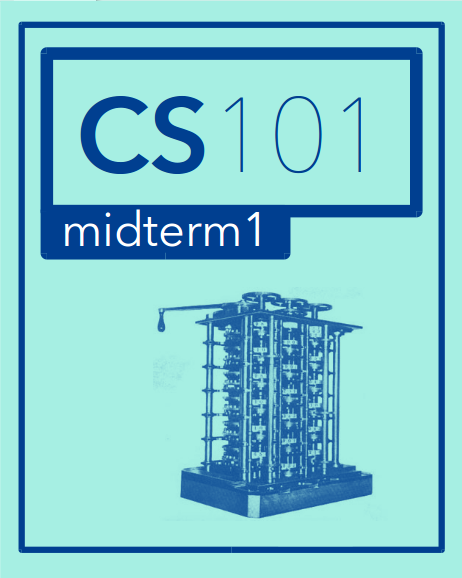
\includegraphics[width=2in]{../img/midterm1-header.png}
\end{center}

\bigskip
\noindent
\begin{itemize}
\item \textbf{Be sure to enter your \underline{NetID} and \underline{the code below} on your Scantron}.
\item Do not turn this page until instructed to do so.
\item There are 30 questions, worth 1 point each.
\item Each question has only \textbf{one} correct answer.
\item You must not communicate with other students during this test.
\item No books, notes, or electronic devices are permitted.
\item This is a 60-minute exam.
\item There are several different versions of this exam.
\end{itemize}

\bigskip\bigskip
\noindent
\textbf{\Large 1. Fill in your information:}

\bigskip
{\Large\bf
\begin{tabular}{ll}
Full Name: & \underbar{\hskip 8cm} \\[0.5em]
UIN (Student Number): & \underbar{\hskip 8cm} \\[0.5em]
NetID: & \underbar{\hskip 8cm}
\end{tabular}
}

\bigskip
\bigskip
\noindent
\textbf{\Large 2. Fill in the following answers on the Scantron form:}

%%%%%%%%%%%%%%%%%%%%%%%%%%%%%%%%%%%%%%%%%%%%%%%%%%%%%%%%%
%%%%%%%%%%%%%%%%%%%%%%%%%%%%%%%%%%%%%%%%%%%%%%%%%%%%%%%%%

\begin{enumerate}
\item[92.] E
\item[93.] C
\item[94.] A
\item[95.] E
\item[96.] A
\end{enumerate}

\newpage

% Zone 1


%%%%%%%%%%%%%%%%%%%%%%%%%%%%%%%%%%%%%%%%%%%%%%%%%%%%%%%%%



\newpage
\noindent
1. (1 point)
Consider the following program:
\begin{verbatim}
x=str(1.2)*2
\end{verbatim}
What is the \textbf{value} of \texttt{x} after this program is executed?


\begin{enumerate}
\item[(A)]
None of the other answers are correct.

\item[(B)]
\begin{verbatim}"2.4"\end{verbatim}

\item[(C)]
\begin{verbatim}2.4\end{verbatim}

\item[(D)]
\begin{verbatim}"1.2*2"\end{verbatim}

\item[(E)] $\bigstar$ 
\begin{verbatim}"1.21.2"\end{verbatim}

\end{enumerate}

\vspace*{2em}
\hrule
\vspace{2em}

\noindent {\bf Solution.} 
\vspace{2em}
\hrule height 2pt


\newpage
\noindent
2. (1 point)
Consider the following program:
\begin{verbatim}
a=["A","C","C","I","O"]
a.sort()
a[0]=a[-1]
x=""
for e in a:
    x=x+e
\end{verbatim}
What is the \textbf{value} of \texttt{x} after this program is executed?


\begin{enumerate}
\item[(A)]
\begin{verbatim}"ICCOI"\end{verbatim}

\item[(B)]
\begin{verbatim}"ACCOA"\end{verbatim}

\item[(C)]
\begin{verbatim}"ACCIA"\end{verbatim}

\item[(D)]
None of the other answers are correct.

\item[(E)] $\bigstar$ 
\begin{verbatim}"OCCIO"\end{verbatim}

\end{enumerate}

\vspace*{2em}
\hrule
\vspace{2em}

\noindent {\bf Solution.} 
\vspace{2em}
\hrule height 2pt


\newpage
\noindent
3. (1 point)
Consider the following program:
\begin{verbatim}
s="TRIS %i"
t="ISEU"
x=s % len(t)
\end{verbatim}
What is the \textbf{type} of \texttt{x} after this program is executed?


\begin{enumerate}
\item[(A)] $\bigstar$ 
\begin{verbatim}String\end{verbatim}

\item[(B)]
\begin{verbatim}Float\end{verbatim}

\item[(C)]
\begin{verbatim}None\end{verbatim}

\item[(D)]
\begin{verbatim}Integer\end{verbatim}

\item[(E)]
\begin{verbatim}Boolean\end{verbatim}

\end{enumerate}

\vspace*{2em}
\hrule
\vspace{2em}

\noindent {\bf Solution.} 
\vspace{2em}
\hrule height 2pt


\newpage
\noindent
4. (1 point)
Consider the following program.
\begin{verbatim}
x=0
i=1
while(i*i)<=9:
    x=x+(i*i)
    i=i+1
\end{verbatim}
After it is run, what is the final \textbf{value} of \texttt{x}?


\begin{enumerate}
\item[(A)] $\bigstar$ 
\begin{verbatim}14\end{verbatim}

\item[(B)]
\begin{verbatim}5\end{verbatim}

\item[(C)]
\begin{verbatim}30\end{verbatim}

\item[(D)]
\begin{verbatim}3\end{verbatim}

\item[(E)]
\begin{verbatim}4\end{verbatim}

\end{enumerate}

\vspace*{2em}
\hrule
\vspace{2em}

\noindent {\bf Solution.} 
\vspace{2em}
\hrule height 2pt


\newpage
\noindent
5. (1 point)
Consider the following incomplete function.
\begin{verbatim}
def ismultiple(m,n):
    if ???:
        return False
    else:
        return True
\end{verbatim}
The function is intended to return True if the input parameter m is a multiple of parameter n and False otherwise. For example, \verb|ismultiple(4,2)| should return \verb|True|, but \verb|ismultiple(5,3)| should return \verb|False|. What should replace the three question marks to complete the function?


\begin{enumerate}
\item[(A)] $\bigstar$ 
\begin{verbatim}(m % n) != 0 \end{verbatim}

\item[(B)]
\begin{verbatim}(n % m) == 0 \end{verbatim}

\item[(C)]
\begin{verbatim}(m // n) != 0 \end{verbatim}

\item[(D)]
\begin{verbatim}(n // m) == 0 \end{verbatim}

\end{enumerate}

\vspace*{2em}
\hrule
\vspace{2em}

\noindent {\bf Solution.} 
\vspace{2em}
\hrule height 2pt


\newpage
\noindent
6. (1 point)
Consider the following Python program.
\begin{verbatim}
e=[1,3,5,7,9,11]
d=[0,0,0]
for i in range(0,len(e)):
    d[i%3]+=e[i]
x=d[1]
\end{verbatim}
After it is run, what is the final \textbf{value} of \texttt{x}?


\begin{enumerate}
\item[(A)]
\begin{verbatim}8\end{verbatim}

\item[(B)]
\begin{verbatim}3\end{verbatim}

\item[(C)]
\begin{verbatim}0\end{verbatim}

\item[(D)]
\begin{verbatim}16\end{verbatim}

\item[(E)] $\bigstar$ 
\begin{verbatim}12\end{verbatim}

\end{enumerate}

\vspace*{2em}
\hrule
\vspace{2em}

\noindent {\bf Solution.} 
\vspace{2em}
\hrule height 2pt


\newpage
\noindent
7. (1 point)
Evaluate the following expression:
\begin{verbatim}
len("ABCDE"[1:4])
\end{verbatim}
What value is produced?


\begin{enumerate}
\item[(A)]
5

\item[(B)]
4

\item[(C)] $\bigstar$ 
3

\item[(D)]
1

\end{enumerate}

\vspace*{2em}
\hrule
\vspace{2em}

\noindent {\bf Solution.} 
\vspace{2em}
\hrule height 2pt


\newpage
\noindent
8. (1 point)
Consider the following program:
\begin{verbatim}
x=[1,2,3]
def f(a):
    s=""
    a.append(4)
    for i in a:
        s+=str(i)
    return s

x.append(f(x))
\end{verbatim}
What is the \textbf{value} of \texttt{x} after this program is executed?


\begin{enumerate}
\item[(A)]
\begin{verbatim}[1, 2, 3, '1234']\end{verbatim}

\item[(B)] $\bigstar$ 
\begin{verbatim}[1, 2, 3, 4, '1234']\end{verbatim}

\item[(C)]
\begin{verbatim}[1, 2, 3]\end{verbatim}

\item[(D)]
\begin{verbatim}[1, 2, 3, '123']\end{verbatim}

\item[(E)]
\begin{verbatim}[1, 2, 3, 10]\end{verbatim}

\end{enumerate}

\vspace*{2em}
\hrule
\vspace{2em}

\noindent {\bf Solution.} 
\vspace{2em}
\hrule height 2pt


\newpage
\noindent
9. (1 point)
Consider the following program:
\begin{verbatim}
x=0
for i in range(2,7):
    if i%3==0:
        x+=3
    elif i%2==0:
        x+=2
    else:
        x+=1
\end{verbatim}
What is the \textbf{value} of \texttt{x} after this program is executed?


\begin{enumerate}
\item[(A)]
\begin{verbatim}14\end{verbatim}

\item[(B)] $\bigstar$ 
\begin{verbatim}11\end{verbatim}

\item[(C)]
\begin{verbatim}12\end{verbatim}

\item[(D)]
\begin{verbatim}10\end{verbatim}

\item[(E)]
\begin{verbatim}13\end{verbatim}

\end{enumerate}

\vspace*{2em}
\hrule
\vspace{2em}

\noindent {\bf Solution.} 
\vspace{2em}
\hrule height 2pt


\newpage
\noindent
10. (1 point)
Consider the following program:
\begin{verbatim}
x=[2,3,4,5,6,7,8,9]
x=x[2:-2]
i=1
while i <= 3:
    x[i]+=1
    i+=1
\end{verbatim}
What is the \textbf{value} of \texttt{x} after this program is executed?


\begin{enumerate}
\item[(A)]
\begin{verbatim}[3, 4, 6, 7, 8]\end{verbatim}

\item[(B)]
\begin{verbatim}[2, 4, 6, 6]\end{verbatim}

\item[(C)]
\begin{verbatim}[4, 6, 7, 7]\end{verbatim}

\item[(D)] $\bigstar$ 
\begin{verbatim}[4, 6, 7, 8]\end{verbatim}

\item[(E)]
\begin{verbatim}[4, 6, 7]\end{verbatim}

\end{enumerate}

\vspace*{2em}
\hrule
\vspace{2em}

\noindent {\bf Solution.} 
\vspace{2em}
\hrule height 2pt


\newpage
\noindent
11. (1 point)
For this problem, you should compose a function which accomplishes a given task using the available code blocks arranged in the correct functional order.  \emph{We ignore indentation for this problem.}

\texttt{find\_max} should accept a \texttt{list} and return the value of the maximum item in the \texttt{list}.  (\texttt{None} is always the lowest value in any numeric comparison, so you may use it as an initializer.)

\begin{verbatim}
def find_max(my_list):
\end{verbatim}

\begin{enumerate}[1]
\item \texttt{max\_val = i}
\item \texttt{max\_val = None}
\item \texttt{for i in range(len(my\_list)):}
\item \texttt{if i > max\_val:}
\item \texttt{max\_val = my\_list[i]}
\item \texttt{return max\_val}
\item \texttt{for i in range(my\_list):}
\item \texttt{if my\_list[i] > max\_val:}
\item \texttt{print(max\_val)}
\end{enumerate}



\begin{enumerate}
\item[(A)]
2, 3, 4, 1, 6

\item[(B)]
3, 2, 8, 5, 9

\item[(C)]
2, 3, 8, 1, 6

\item[(D)] $\bigstar$ 
2, 3, 8, 5, 6

\item[(E)]
2, 7, 4, 5, 6

\end{enumerate}

\vspace*{2em}
\hrule
\vspace{2em}

\noindent {\bf Solution.} 
\vspace{2em}
\hrule height 2pt


\newpage
\noindent
12. (1 point)
Consider the following program:
\begin{verbatim}
a=3
b=4
if a==3:
    b=a
elif a==4:
    a=5
else:
    a=b
\end{verbatim}
What is the \textbf{value} of a after this program is executed?


\begin{enumerate}
\item[(A)]
None of the other answers are correct.

\item[(B)]
\begin{verbatim}5\end{verbatim}

\item[(C)] $\bigstar$ 
\begin{verbatim}3\end{verbatim}

\item[(D)]
\begin{verbatim}7\end{verbatim}

\item[(E)]
\begin{verbatim}4\end{verbatim}

\end{enumerate}

\vspace*{2em}
\hrule
\vspace{2em}

\noindent {\bf Solution.} 
\vspace{2em}
\hrule height 2pt


\newpage
\noindent
13. (1 point)
Consider the following program:
\begin{verbatim}
s="ECTOR"
t="GAWAIN"
x=(len(s)+len(t)) < 4 and s in t
\end{verbatim}
What is the \textbf{type} of \texttt{x} after this program is executed?


\begin{enumerate}
\item[(A)]
\begin{verbatim}Float\end{verbatim}

\item[(B)] $\bigstar$ 
\begin{verbatim}Boolean\end{verbatim}

\item[(C)]
\begin{verbatim}Integer\end{verbatim}

\item[(D)]
\begin{verbatim}String\end{verbatim}

\item[(E)]
\begin{verbatim}None\end{verbatim}

\end{enumerate}

\vspace*{2em}
\hrule
\vspace{2em}

\noindent {\bf Solution.} 
\vspace{2em}
\hrule height 2pt


\newpage
\noindent
14. (1 point)
Consider the following incomplete Python program.
\begin{verbatim}
s="".join(["2","2","0","1"])
x=0
for i in range(len(s)-1):
    x+=int(???)
\end{verbatim}
What should replace the three question marks so the resulting value of \texttt{x} is 43?


\begin{enumerate}
\item[(A)]
\begin{verbatim}s[i:i+1]\end{verbatim}

\item[(B)]
\begin{verbatim}s[i:i-1]\end{verbatim}

\item[(C)]
\begin{verbatim}s[i+1:i+2]\end{verbatim}

\item[(D)] $\bigstar$ 
\begin{verbatim}s[i:i+2]\end{verbatim}

\end{enumerate}

\vspace*{2em}
\hrule
\vspace{2em}

\noindent {\bf Solution.} 
\vspace{2em}
\hrule height 2pt


\newpage
\noindent
15. (1 point)
Consider the following program.
\begin{verbatim}
x=[]
for j in range(0,5):
    if (j%2)==0:
        x.append("-")
    if (j%5)==0:
        x.append("*")
\end{verbatim}
After it is run, what is the final \textbf{value} of \texttt{x}?


\begin{enumerate}
\item[(A)]
\begin{verbatim}["-","*","-"]\end{verbatim}

\item[(B)] $\bigstar$ 
\begin{verbatim}["-","*","-","-"]\end{verbatim}

\item[(C)]
\begin{verbatim}["-","-","*"]\end{verbatim}

\item[(D)]
None of the other answers are correct.

\item[(E)]
\begin{verbatim}["*","-","*","*"]\end{verbatim}

\end{enumerate}

\vspace*{2em}
\hrule
\vspace{2em}

\noindent {\bf Solution.} 
\vspace{2em}
\hrule height 2pt


\newpage
\noindent
16. (1 point)
Consider the following program:
\begin{verbatim}
s="-B-O-R-S-"
x=s.split("-")[2:-2]
\end{verbatim}
What is the \textbf{value} of \texttt{x} after this program is executed?


\begin{enumerate}
\item[(A)]
\begin{verbatim}None\end{verbatim}

\item[(B)]
\begin{verbatim}''\end{verbatim}

\item[(C)]
\begin{verbatim}False\end{verbatim}

\item[(D)]
\begin{verbatim}'ORS'\end{verbatim}

\item[(E)] $\bigstar$ 
\begin{verbatim}['O', 'R']\end{verbatim}

\end{enumerate}

\vspace*{2em}
\hrule
\vspace{2em}

\noindent {\bf Solution.} 
\vspace{2em}
\hrule height 2pt


\newpage
\noindent
17. (1 point)
Consider the following incomplete program.
\begin{verbatim}
sum=0
???:
    sum=sum+i

\end{verbatim}
The program is intended to sum all of the integers between 1 and 100 (inclusive). What should replace the three question marks to complete the program?


\begin{enumerate}
\item[(A)] $\bigstar$ 
\begin{verbatim}for i in range(1,101) \end{verbatim}

\item[(B)]
\begin{verbatim}while i<=100 \end{verbatim}

\item[(C)]
\begin{verbatim}while i in range(100)\end{verbatim}

\item[(D)]
\begin{verbatim}for i in range(0,100)\end{verbatim}

\end{enumerate}

\vspace*{2em}
\hrule
\vspace{2em}

\noindent {\bf Solution.} 
\vspace{2em}
\hrule height 2pt


\newpage
\noindent
18. (1 point)
What is the result of the following expression?
\begin{verbatim}
[ 1, 2, 3 ] * 3
\end{verbatim}


\begin{enumerate}
\item[(A)] $\bigstar$ 
\begin{verbatim}[1, 2, 3, 1, 2, 3, 1, 2, 3]\end{verbatim}

\item[(B)]
\begin{verbatim}(3, 6, 9)\end{verbatim}

\item[(C)]
\begin{verbatim}[3.0, 6.0, 9.0]\end{verbatim}

\item[(D)]
\begin{verbatim}[3, 6, 9]\end{verbatim}

\item[(E)]
\begin{verbatim}[1.0, 2.0, 3.0, 1.0, 2.0, 3.0, 1.0, 2.0, 3.0]\end{verbatim}

\end{enumerate}

\vspace*{2em}
\hrule
\vspace{2em}

\noindent {\bf Solution.} 
\vspace{2em}
\hrule height 2pt


\newpage
\noindent
19. (1 point)
Consider the following program:
\begin{verbatim}
s="Calvin"
i=0
x=-1
while i<len(s):
    if s[i]=='b':
        x=i
    i+=1
\end{verbatim}
What is the \textbf{value} of \texttt{x} after this program is executed?


\begin{enumerate}
\item[(A)]
\begin{verbatim}0\end{verbatim}

\item[(B)]
\begin{verbatim}5\end{verbatim}

\item[(C)]
\begin{verbatim}6\end{verbatim}

\item[(D)]
\begin{verbatim}3\end{verbatim}

\item[(E)] $\bigstar$ 
\begin{verbatim}-1\end{verbatim}

\end{enumerate}

\vspace*{2em}
\hrule
\vspace{2em}

\noindent {\bf Solution.} 
\vspace{2em}
\hrule height 2pt


\newpage
\noindent
20. (1 point)
Consider the following program:
\begin{verbatim}
x=2
a=6
if (a%3)==2:
    x=x**3
elif(a%3)==1:
    x=x**2
else:
    x=x**1
\end{verbatim}
What is the \textbf{value} of \texttt{x} after this program is executed?


\begin{enumerate}
\item[(A)]
None of the other answers are correct.

\item[(B)]
\begin{verbatim}8\end{verbatim}

\item[(C)]
\begin{verbatim}4\end{verbatim}

\item[(D)] $\bigstar$ 
\begin{verbatim}2\end{verbatim}

\item[(E)]
\begin{verbatim}16\end{verbatim}

\end{enumerate}

\vspace*{2em}
\hrule
\vspace{2em}

\noindent {\bf Solution.} 
\vspace{2em}
\hrule height 2pt


\newpage
\noindent
21. (1 point)
Evaluate the following expression:
\begin{verbatim}
[1,2]+[len("3")]
\end{verbatim}
What value is produced?


\begin{enumerate}
\item[(A)]
\begin{verbatim}[1,2,1,2,1,2]\end{verbatim}

\item[(B)]
\begin{verbatim}[1,2,3]\end{verbatim}

\item[(C)] $\bigstar$ 
\begin{verbatim}[1,2,1]\end{verbatim}

\item[(D)]
\begin{verbatim}[1,2,"3"]\end{verbatim}

\end{enumerate}

\vspace*{2em}
\hrule
\vspace{2em}

\noindent {\bf Solution.} 
\vspace{2em}
\hrule height 2pt


\newpage
\noindent
22. (1 point)
Consider the following program.
\begin{verbatim}
s="BBCAA"
x=0
y=len(s)-1
while s[x]!=s[y] and x<len(s):
    x+=1
    y-=1
\end{verbatim}
After it is run, what is the final \textbf{value} of \texttt{x}?


\begin{enumerate}
\item[(A)]
\begin{verbatim}4\end{verbatim}

\item[(B)]
\begin{verbatim}1\end{verbatim}

\item[(C)]
\begin{verbatim}0\end{verbatim}

\item[(D)]
\begin{verbatim}3\end{verbatim}

\item[(E)] $\bigstar$ 
\begin{verbatim}2\end{verbatim}

\end{enumerate}

\vspace*{2em}
\hrule
\vspace{2em}

\noindent {\bf Solution.} 
\vspace{2em}
\hrule height 2pt


\newpage
\noindent
23. (1 point)
Consider the following program.
\begin{verbatim}
def artificing(s):
    return s+"%i" % 2
    return s*2
    return s

s=artificing("MERLIN")
\end{verbatim}
After it is run, what is the final \textbf{value} of s?


\begin{enumerate}
\item[(A)] $\bigstar$ 
\begin{verbatim}"MERLIN2"\end{verbatim}

\item[(B)]
\begin{verbatim}0\end{verbatim}

\item[(C)]
\begin{verbatim}"MERLIN%i"\end{verbatim}

\item[(D)]
\begin{verbatim}"MERLINMERLIN"\end{verbatim}

\item[(E)]
\begin{verbatim}None\end{verbatim}

\end{enumerate}

\vspace*{2em}
\hrule
\vspace{2em}

\noindent {\bf Solution.} 
\vspace{2em}
\hrule height 2pt


\newpage
\noindent
24. (1 point)
Consider the following program:
\begin{verbatim}
def fix(s):
    a=list(s)
    a.sort()
    return ''.join(a)

x=["one","two","eleven","twelve"]
s1=fix(x[0]+x[-1])
s2=fix(x[1]+x[-2])

if s1<s2:
    x.sort()
elif s1==s2:
    x.reverse()
else:
    x.append("six")
\end{verbatim}
What is the \textbf{value} of \texttt{x} after this program is executed?


\begin{enumerate}
\item[(A)] $\bigstar$ 
\begin{verbatim}['twelve', 'eleven', 'two', 'one']\end{verbatim}

\item[(B)]
\begin{verbatim}['one', 'two', 'eleven', 'twelve', 'six']\end{verbatim}

\item[(C)]
\begin{verbatim}['two', 'twelve', 'one', 'eleven', 'six']\end{verbatim}

\item[(D)]
\begin{verbatim}['one', 'two', 'eleven', 'twelve']\end{verbatim}

\item[(E)]
\begin{verbatim}['eleven', 'one', 'twelve', 'two']\end{verbatim}

\end{enumerate}

\vspace*{2em}
\hrule
\vspace{2em}

\noindent {\bf Solution.} 
\vspace{2em}
\hrule height 2pt


\newpage
\noindent
25. (1 point)
Consider the following program:
\begin{verbatim}
x="KING ARTHUR-MORGANA LEFAY-SIR BEDIVERE".split("-")
y=x
y.reverse()
\end{verbatim}
What is the \textbf{value} of \texttt{x} after this program is executed?


\begin{enumerate}
\item[(A)]
\begin{verbatim}['KING ARTHUR', 'MORGANA LEFAY', 'SIR BEDIVERE']\end{verbatim}

\item[(B)]
\begin{verbatim}None\end{verbatim}

\item[(C)]
\begin{verbatim}['BEDIVERE', 'LEFAY-SIR', 'ARTHUR-MORGANA', 'KING']\end{verbatim}

\item[(D)]
\begin{verbatim}['KING', 'ARTHUR-MORGANA', 'LEFAY-SIR', 'BEDIVERE']\end{verbatim}

\item[(E)] $\bigstar$ 
\begin{verbatim}['SIR BEDIVERE', 'MORGANA LEFAY', 'KING ARTHUR']\end{verbatim}

\end{enumerate}

\vspace*{2em}
\hrule
\vspace{2em}

\noindent {\bf Solution.} 
\vspace{2em}
\hrule height 2pt


\newpage
\noindent
26. (1 point)
How can the following mathematical equation be implemented as a Python expression? Assume \verb|a|, \verb|b|, and \verb|sin| have already been defined.
$$a \sin(a^b - b)$$


\begin{enumerate}
\item[(A)]
None of the other answers are correct.

\item[(B)] $\bigstar$ 
\begin{verbatim}a*sin(a**b - b)\end{verbatim}

\item[(C)]
\begin{verbatim}a*sin(b^a - b)\end{verbatim}

\item[(D)]
\begin{verbatim}a sin(a**b - b)\end{verbatim}

\item[(E)]
\begin{verbatim}a*sin(a^b - b)\end{verbatim}

\end{enumerate}

\vspace*{2em}
\hrule
\vspace{2em}

\noindent {\bf Solution.} 
\vspace{2em}
\hrule height 2pt


\newpage
\noindent
27. (1 point)
Consider the following program:
\begin{verbatim}
i=2
x=3
while i < 7:
    x+=i
    i+=2
\end{verbatim}
What is the \textbf{value} of \texttt{x} after this program is executed?


\begin{enumerate}
\item[(A)]
\begin{verbatim}11\end{verbatim}

\item[(B)]
\begin{verbatim}14\end{verbatim}

\item[(C)]
\begin{verbatim}13\end{verbatim}

\item[(D)]
\begin{verbatim}12\end{verbatim}

\item[(E)] $\bigstar$ 
\begin{verbatim}15\end{verbatim}

\end{enumerate}

\vspace*{2em}
\hrule
\vspace{2em}

\noindent {\bf Solution.} 
\vspace{2em}
\hrule height 2pt


\newpage
\noindent
28. (1 point)
Consider the following program:
\begin{verbatim}
a=["merlin","sir agravaine","king pellinore"]
b=[ ]
for i in range(1,3):
    b.append(a[0-i].title())
\end{verbatim}
What is the \textbf{value} of b after this program is executed?


\begin{enumerate}
\item[(A)]
\begin{verbatim}['Sir Agravaine', 'King Pellinore']\end{verbatim}

\item[(B)]
\begin{verbatim}['King Pellinore', 'Sir Agravaine', 'Merlin']\end{verbatim}

\item[(C)]
\begin{verbatim}[ ]\end{verbatim}

\item[(D)] $\bigstar$ 
\begin{verbatim}['King Pellinore', 'Sir Agravaine']\end{verbatim}

\item[(E)]
\begin{verbatim}['Merlin', 'King Pellinore', 'Sir Agravaine']\end{verbatim}

\end{enumerate}

\vspace*{2em}
\hrule
\vspace{2em}

\noindent {\bf Solution.} 
\vspace{2em}
\hrule height 2pt


\newpage
\noindent
29. (1 point)
Consider the following program.
\begin{verbatim}
kay = 2
wart = 3

def knight(kay,wart):
    wart += 2
    kay += 3
    return wart + kay

wart = knight(kay, kay) + knight(wart, wart)
\end{verbatim}
After it is run, what is the final \textbf{value} of \texttt{wart}?


\begin{enumerate}
\item[(A)]
\begin{verbatim}2\end{verbatim}

\item[(B)]
\begin{verbatim}3\end{verbatim}

\item[(C)]
\begin{verbatim}5\end{verbatim}

\item[(D)] $\bigstar$ 
None of the other answers are correct.

\end{enumerate}

\vspace*{2em}
\hrule
\vspace{2em}

\noindent {\bf Solution.} 
\vspace{2em}
\hrule height 2pt


\newpage
\noindent
30. (1 point)
Consider the following program:
\begin{verbatim}
pi="3.14159"
e="2.71828"
x=pi in pi*len(e)
\end{verbatim}
What is the \textbf{type} of \texttt{x} after this program is executed?


\begin{enumerate}
\item[(A)]
\begin{verbatim}Integer\end{verbatim}

\item[(B)] $\bigstar$ 
\begin{verbatim}Boolean\end{verbatim}

\item[(C)]
\begin{verbatim}None\end{verbatim}

\item[(D)]
\begin{verbatim}Float\end{verbatim}

\item[(E)]
\begin{verbatim}String\end{verbatim}

\end{enumerate}

\vspace*{2em}
\hrule
\vspace{2em}

\noindent {\bf Solution.} 
\vspace{2em}
\hrule height 2pt

%%%%%%%%%%%%%%%%%%%%%%%%%%%%%%%%%%%%%%%%%%%%%%%%%%%%%%%%%%%%%%%%%%%%%%
%%%%%%%%%%%%%%%%%%%%%%%%%%%%%%%%%%%%%%%%%%%%%%%%%%%%%%%%%%%%%%%%%%%%%%
%%%%%%%%%%%%%%%%%%%%%%%%%%%%%%%%%%%%%%%%%%%%%%%%%%%%%%%%%%%%%%%%%%%%%%
%%%%%%%%%%%%%%%%%%%%%%%%%%%%%%%%%%%%%%%%%%%%%%%%%%%%%%%%%%%%%%%%%%%%%%
% Exam number 16

\message{Exam 16/50}
\cleardoublepage
\setcounter{page}{1}


\begin{center}
%\textbf{\Large CS 101 Midterm \#1}
%
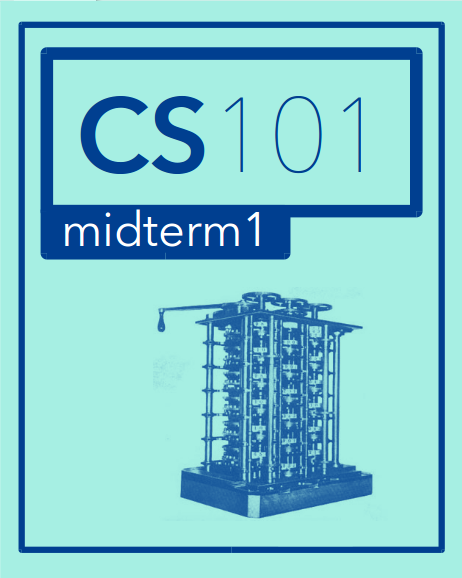
\includegraphics[width=2in]{../img/midterm1-header.png}
\end{center}

\bigskip
\noindent
\begin{itemize}
\item \textbf{Be sure to enter your \underline{NetID} and \underline{the code below} on your Scantron}.
\item Do not turn this page until instructed to do so.
\item There are 30 questions, worth 1 point each.
\item Each question has only \textbf{one} correct answer.
\item You must not communicate with other students during this test.
\item No books, notes, or electronic devices are permitted.
\item This is a 60-minute exam.
\item There are several different versions of this exam.
\end{itemize}

\bigskip\bigskip
\noindent
\textbf{\Large 1. Fill in your information:}

\bigskip
{\Large\bf
\begin{tabular}{ll}
Full Name: & \underbar{\hskip 8cm} \\[0.5em]
UIN (Student Number): & \underbar{\hskip 8cm} \\[0.5em]
NetID: & \underbar{\hskip 8cm}
\end{tabular}
}

\bigskip
\bigskip
\noindent
\textbf{\Large 2. Fill in the following answers on the Scantron form:}

%%%%%%%%%%%%%%%%%%%%%%%%%%%%%%%%%%%%%%%%%%%%%%%%%%%%%%%%%
%%%%%%%%%%%%%%%%%%%%%%%%%%%%%%%%%%%%%%%%%%%%%%%%%%%%%%%%%

\begin{enumerate}
\item[92.] A
\item[93.] D
\item[94.] A
\item[95.] B
\item[96.] D
\end{enumerate}

\newpage

% Zone 1


%%%%%%%%%%%%%%%%%%%%%%%%%%%%%%%%%%%%%%%%%%%%%%%%%%%%%%%%%



\newpage
\noindent
1. (1 point)
Consider the following program:
\begin{verbatim}
def fix(s):
    a=list(s)
    a.sort()
    return ''.join(a)

x=["one","two","eleven","twelve"]
s1=fix(x[0]+x[-1])
s2=fix(x[1]+x[-2])

if s1==s2:
    x.sort()
elif s1<s2:
    x.reverse()
else:
    x.append("six")
\end{verbatim}
What is the \textbf{value} of \texttt{x} after this program is executed?


\begin{enumerate}
\item[(A)]
\begin{verbatim}['twelve', 'eleven', 'two', 'one']\end{verbatim}

\item[(B)]
\begin{verbatim}['one', 'two', 'eleven', 'twelve']\end{verbatim}

\item[(C)] $\bigstar$ 
\begin{verbatim}['eleven', 'one', 'twelve', 'two']\end{verbatim}

\item[(D)]
\begin{verbatim}['two', 'twelve', 'one', 'eleven', 'six']\end{verbatim}

\item[(E)]
\begin{verbatim}['one', 'two', 'eleven', 'twelve', 'six']\end{verbatim}

\end{enumerate}

\vspace*{2em}
\hrule
\vspace{2em}

\noindent {\bf Solution.} 
\vspace{2em}
\hrule height 2pt


\newpage
\noindent
2. (1 point)
Evaluate the following expression:
\begin{verbatim}
len("ABCD"[0:3])
\end{verbatim}
What value is produced?


\begin{enumerate}
\item[(A)]
2

\item[(B)] $\bigstar$ 
3

\item[(C)]
4

\item[(D)]
1

\end{enumerate}

\vspace*{2em}
\hrule
\vspace{2em}

\noindent {\bf Solution.} 
\vspace{2em}
\hrule height 2pt


\newpage
\noindent
3. (1 point)
Consider the following program.
\begin{verbatim}
kay = 2
wart = 3

def knight(kay,wart):
    wart += 2
    kay += 3
    return wart + kay

wart = knight(kay, kay) + knight(wart, wart)
\end{verbatim}
After it is run, what is the final \textbf{value} of \texttt{wart}?


\begin{enumerate}
\item[(A)]
\begin{verbatim}5\end{verbatim}

\item[(B)] $\bigstar$ 
None of the other answers are correct.

\item[(C)]
\begin{verbatim}3\end{verbatim}

\item[(D)]
\begin{verbatim}2\end{verbatim}

\end{enumerate}

\vspace*{2em}
\hrule
\vspace{2em}

\noindent {\bf Solution.} 
\vspace{2em}
\hrule height 2pt


\newpage
\noindent
4. (1 point)
Consider the following program:
\begin{verbatim}
s="ECTOR"
t="GAWAIN"
x=(len(s)/(len(t)-1))+1
\end{verbatim}
What is the \textbf{type} of \texttt{x} after this program is executed?


\begin{enumerate}
\item[(A)] $\bigstar$ 
\begin{verbatim}Float\end{verbatim}

\item[(B)]
\begin{verbatim}Boolean\end{verbatim}

\item[(C)]
\begin{verbatim}Integer\end{verbatim}

\item[(D)]
\begin{verbatim}String\end{verbatim}

\item[(E)]
\begin{verbatim}None\end{verbatim}

\end{enumerate}

\vspace*{2em}
\hrule
\vspace{2em}

\noindent {\bf Solution.} 
\vspace{2em}
\hrule height 2pt


\newpage
\noindent
5. (1 point)
Consider the following program:
\begin{verbatim}
x=3
a=5
if (a%3)==2:
    x=x**3
elif(a%3)==1:
    x=x**2
else:
    x=x**1
\end{verbatim}
What is the \textbf{value} of \texttt{x} after this program is executed?


\begin{enumerate}
\item[(A)] $\bigstar$ 
\begin{verbatim}27\end{verbatim}

\item[(B)]
\begin{verbatim}1\end{verbatim}

\item[(C)]
\begin{verbatim}9\end{verbatim}

\item[(D)]
\begin{verbatim}3\end{verbatim}

\item[(E)]
None of the other answers are correct.

\end{enumerate}

\vspace*{2em}
\hrule
\vspace{2em}

\noindent {\bf Solution.} 
\vspace{2em}
\hrule height 2pt


\newpage
\noindent
6. (1 point)
Consider the following program:
\begin{verbatim}
a=3
b=4
if a!=b:
    a=b
elif a==4:
    a=5
else:
    b=a
\end{verbatim}
What is the \textbf{value} of a after this program is executed?


\begin{enumerate}
\item[(A)]
\begin{verbatim}5\end{verbatim}

\item[(B)]
\begin{verbatim}3\end{verbatim}

\item[(C)]
\begin{verbatim}7\end{verbatim}

\item[(D)]
None of the other answers are correct.

\item[(E)] $\bigstar$ 
\begin{verbatim}4\end{verbatim}

\end{enumerate}

\vspace*{2em}
\hrule
\vspace{2em}

\noindent {\bf Solution.} 
\vspace{2em}
\hrule height 2pt


\newpage
\noindent
7. (1 point)
Consider the following program.
\begin{verbatim}
x=[]
for j in range(0,5):
    if (j%2)==0:
        x.append("-")
    if (j%5)==0:
        x.append("*")
\end{verbatim}
After it is run, what is the final \textbf{value} of \texttt{x}?


\begin{enumerate}
\item[(A)] $\bigstar$ 
\begin{verbatim}["-","*","-","-"]\end{verbatim}

\item[(B)]
None of the other answers are correct.

\item[(C)]
\begin{verbatim}["*","-","*","*"]\end{verbatim}

\item[(D)]
\begin{verbatim}["-","*","-"]\end{verbatim}

\item[(E)]
\begin{verbatim}["-","-","*"]\end{verbatim}

\end{enumerate}

\vspace*{2em}
\hrule
\vspace{2em}

\noindent {\bf Solution.} 
\vspace{2em}
\hrule height 2pt


\newpage
\noindent
8. (1 point)
Consider the following incomplete Python program.
\begin{verbatim}
s="".join(["1","0","2","1"])
x=0
for i in range(len(s)-1):
    x+=int(???)
\end{verbatim}
What should replace the three question marks so the resulting value of \texttt{x} is 33?


\begin{enumerate}
\item[(A)] $\bigstar$ 
\begin{verbatim}s[i:i+2]\end{verbatim}

\item[(B)]
\begin{verbatim}s[i:i+1]\end{verbatim}

\item[(C)]
\begin{verbatim}s[i:i-1]\end{verbatim}

\item[(D)]
\begin{verbatim}s[i+1:i+2]\end{verbatim}

\end{enumerate}

\vspace*{2em}
\hrule
\vspace{2em}

\noindent {\bf Solution.} 
\vspace{2em}
\hrule height 2pt


\newpage
\noindent
9. (1 point)
Consider the following incomplete function.
\begin{verbatim}
def ismultiple(m,n):
    if ???:
        return False
    else:
        return True
\end{verbatim}
The function is intended to return True if the input parameter m is a multiple of parameter n and False otherwise. For example, \verb|ismultiple(4,2)| should return \verb|True|, but \verb|ismultiple(5,3)| should return \verb|False|. What should replace the three question marks to complete the function?


\begin{enumerate}
\item[(A)]
\begin{verbatim}(n % m) == 0 \end{verbatim}

\item[(B)]
\begin{verbatim}(m // n) != 0 \end{verbatim}

\item[(C)]
\begin{verbatim}(n // m) == 0 \end{verbatim}

\item[(D)] $\bigstar$ 
\begin{verbatim}(m % n) != 0 \end{verbatim}

\end{enumerate}

\vspace*{2em}
\hrule
\vspace{2em}

\noindent {\bf Solution.} 
\vspace{2em}
\hrule height 2pt


\newpage
\noindent
10. (1 point)
Consider the following incomplete program.
\begin{verbatim}
sum=0
for i in range(0,100):
    ???

\end{verbatim}
The program is intended to sum all of the integers between 1 and 100 (inclusive). What should replace the three question marks to complete the program?


\begin{enumerate}
\item[(A)] $\bigstar$ 
\begin{verbatim}sum=sum+i+1 \end{verbatim}

\item[(B)]
\begin{verbatim}sum=sum+i \end{verbatim}

\item[(C)]
\begin{verbatim}sum=sum+1\end{verbatim}

\item[(D)]
\begin{verbatim}sum+1=sum \end{verbatim}

\end{enumerate}

\vspace*{2em}
\hrule
\vspace{2em}

\noindent {\bf Solution.} 
\vspace{2em}
\hrule height 2pt


\newpage
\noindent
11. (1 point)
How can the following mathematical equation be implemented as a Python expression? Assume \verb|a|, \verb|b|, and \verb|cos| have already been defined.
$$a^b \cos(a - b)$$


\begin{enumerate}
\item[(A)]
\begin{verbatim}(a^b)*cos(a-b)\end{verbatim}

\item[(B)]
\begin{verbatim}(a**b)cos(a-b)\end{verbatim}

\item[(C)]
\begin{verbatim}(b^a)cos(a-b)\end{verbatim}

\item[(D)]
None of the other answers are correct.

\item[(E)] $\bigstar$ 
\begin{verbatim}(a**b)*cos(a-b)\end{verbatim}

\end{enumerate}

\vspace*{2em}
\hrule
\vspace{2em}

\noindent {\bf Solution.} 
\vspace{2em}
\hrule height 2pt


\newpage
\noindent
12. (1 point)
Consider the following program:
\begin{verbatim}
x=[1,2,3]
def f(a):
    s=""
    a.append(4)
    for i in a:
        s+=str(i)
    return s

x.append(f(x))
\end{verbatim}
What is the \textbf{value} of \texttt{x} after this program is executed?


\begin{enumerate}
\item[(A)] $\bigstar$ 
\begin{verbatim}[1, 2, 3, 4, '1234']\end{verbatim}

\item[(B)]
\begin{verbatim}[1, 2, 3, '1234']\end{verbatim}

\item[(C)]
\begin{verbatim}[1, 2, 3]\end{verbatim}

\item[(D)]
\begin{verbatim}[1, 2, 3, '123']\end{verbatim}

\item[(E)]
\begin{verbatim}[1, 2, 3, 10]\end{verbatim}

\end{enumerate}

\vspace*{2em}
\hrule
\vspace{2em}

\noindent {\bf Solution.} 
\vspace{2em}
\hrule height 2pt


\newpage
\noindent
13. (1 point)
Consider the following program:
\begin{verbatim}
s="-B-O-R-S-"
x=s.split("-")[2:-2]
\end{verbatim}
What is the \textbf{value} of \texttt{x} after this program is executed?


\begin{enumerate}
\item[(A)] $\bigstar$ 
\begin{verbatim}['O', 'R']\end{verbatim}

\item[(B)]
\begin{verbatim}''\end{verbatim}

\item[(C)]
\begin{verbatim}False\end{verbatim}

\item[(D)]
\begin{verbatim}None\end{verbatim}

\item[(E)]
\begin{verbatim}'ORS'\end{verbatim}

\end{enumerate}

\vspace*{2em}
\hrule
\vspace{2em}

\noindent {\bf Solution.} 
\vspace{2em}
\hrule height 2pt


\newpage
\noindent
14. (1 point)
Consider the following program:
\begin{verbatim}
x="KING ARTHUR-MORGANA LEFAY-SIR BEDIVERE".split("-")
y=x
x=y.reverse()
\end{verbatim}
What is the \textbf{value} of \texttt{x} after this program is executed?


\begin{enumerate}
\item[(A)]
\begin{verbatim}['KING ARTHUR', 'MORGANA LEFAY', 'SIR BEDIVERE']\end{verbatim}

\item[(B)] $\bigstar$ 
\begin{verbatim}None\end{verbatim}

\item[(C)]
\begin{verbatim}['BEDIVERE', 'LEFAY-SIR', 'ARTHUR-MORGANA', 'KING']\end{verbatim}

\item[(D)]
\begin{verbatim}['SIR BEDIVERE', 'MORGANA LEFAY', 'KING ARTHUR']\end{verbatim}

\item[(E)]
\begin{verbatim}['KING', 'ARTHUR-MORGANA', 'LEFAY-SIR', 'BEDIVERE']\end{verbatim}

\end{enumerate}

\vspace*{2em}
\hrule
\vspace{2em}

\noindent {\bf Solution.} 
\vspace{2em}
\hrule height 2pt


\newpage
\noindent
15. (1 point)
Consider the following program.
\begin{verbatim}
s="ABCBA"
x=0
y=len(s)-1
while s[x]==s[y] and x<y:
    x+=1
    y-=1
\end{verbatim}
After it is run, what is the final \textbf{value} of \texttt{x}?


\begin{enumerate}
\item[(A)] $\bigstar$ 
\begin{verbatim}2\end{verbatim}

\item[(B)]
\begin{verbatim}3\end{verbatim}

\item[(C)]
\begin{verbatim}4\end{verbatim}

\item[(D)]
\begin{verbatim}0\end{verbatim}

\item[(E)]
\begin{verbatim}1\end{verbatim}

\end{enumerate}

\vspace*{2em}
\hrule
\vspace{2em}

\noindent {\bf Solution.} 
\vspace{2em}
\hrule height 2pt


\newpage
\noindent
16. (1 point)
Consider the following Python program.
\begin{verbatim}
e=[1,3,5,7,9,11]
d=[0,0,0]
for i in range(0,len(e)):
    d[i%3]+=e[i]
x=d[2]
\end{verbatim}
After it is run, what is the final \textbf{value} of \texttt{x}?


\begin{enumerate}
\item[(A)]
\begin{verbatim}12\end{verbatim}

\item[(B)] $\bigstar$ 
\begin{verbatim}16\end{verbatim}

\item[(C)]
\begin{verbatim}0\end{verbatim}

\item[(D)]
\begin{verbatim}7\end{verbatim}

\item[(E)]
\begin{verbatim}8\end{verbatim}

\end{enumerate}

\vspace*{2em}
\hrule
\vspace{2em}

\noindent {\bf Solution.} 
\vspace{2em}
\hrule height 2pt


\newpage
\noindent
17. (1 point)
Consider the following program:
\begin{verbatim}
x=[1,2,3,4,5,6,7,8,9]
x=x[2:-2]
i=1
while i < 3:
    x[i]+=1
    i+=1
\end{verbatim}
What is the \textbf{value} of \texttt{x} after this program is executed?


\begin{enumerate}
\item[(A)]
\begin{verbatim}[2, 4, 5, 5, 6, 7]\end{verbatim}

\item[(B)] $\bigstar$ 
\begin{verbatim}[3, 5, 6, 6, 7]\end{verbatim}

\item[(C)]
\begin{verbatim}[3, 5, 6, 6]\end{verbatim}

\item[(D)]
\begin{verbatim}[3, 5, 6, 6, 7, 8]\end{verbatim}

\item[(E)]
\begin{verbatim}[2, 4, 5, 6, 6, 7]\end{verbatim}

\end{enumerate}

\vspace*{2em}
\hrule
\vspace{2em}

\noindent {\bf Solution.} 
\vspace{2em}
\hrule height 2pt


\newpage
\noindent
18. (1 point)
Evaluate the following expression:
\begin{verbatim}
[1,2]*len("3")
\end{verbatim}
What value is produced?


\begin{enumerate}
\item[(A)]
\begin{verbatim}[1,2,3]\end{verbatim}

\item[(B)] $\bigstar$ 
\begin{verbatim}[1,2]\end{verbatim}

\item[(C)]
\begin{verbatim}[1,2,1]\end{verbatim}

\item[(D)]
\begin{verbatim}[1,2,1,2,1,2]\end{verbatim}

\end{enumerate}

\vspace*{2em}
\hrule
\vspace{2em}

\noindent {\bf Solution.} 
\vspace{2em}
\hrule height 2pt


\newpage
\noindent
19. (1 point)
Consider the following program:
\begin{verbatim}
a=["merlin","sir agravaine","king pellinore"]
b=[ ]
for i in range(0,3):
    b.append(a[0-i].title())
\end{verbatim}
What is the \textbf{value} of b after this program is executed?


\begin{enumerate}
\item[(A)]
\begin{verbatim}['King Pellinore', 'Sir Agravaine']\end{verbatim}

\item[(B)] $\bigstar$ 
\begin{verbatim}['Merlin', 'King Pellinore', 'Sir Agravaine']\end{verbatim}

\item[(C)]
\begin{verbatim}['Sir Agravaine', 'King Pellinore']\end{verbatim}

\item[(D)]
\begin{verbatim}['King Pellinore', 'Sir Agravaine', 'Merlin']\end{verbatim}

\item[(E)]
\begin{verbatim}[ ]\end{verbatim}

\end{enumerate}

\vspace*{2em}
\hrule
\vspace{2em}

\noindent {\bf Solution.} 
\vspace{2em}
\hrule height 2pt


\newpage
\noindent
20. (1 point)
Consider the following program:
\begin{verbatim}
x=0
for i in range(2,7):
    if i%3==0:
        x+=3
    elif i%2==0:
        x+=2
    else:
        x+=1
\end{verbatim}
What is the \textbf{value} of \texttt{x} after this program is executed?


\begin{enumerate}
\item[(A)]
\begin{verbatim}10\end{verbatim}

\item[(B)]
\begin{verbatim}14\end{verbatim}

\item[(C)]
\begin{verbatim}12\end{verbatim}

\item[(D)]
\begin{verbatim}13\end{verbatim}

\item[(E)] $\bigstar$ 
\begin{verbatim}11\end{verbatim}

\end{enumerate}

\vspace*{2em}
\hrule
\vspace{2em}

\noindent {\bf Solution.} 
\vspace{2em}
\hrule height 2pt


\newpage
\noindent
21. (1 point)
Consider the following program:
\begin{verbatim}
pi="3.14159"
e="2.71828"
x=pi in pi*len(e)
\end{verbatim}
What is the \textbf{type} of \texttt{x} after this program is executed?


\begin{enumerate}
\item[(A)] $\bigstar$ 
\begin{verbatim}Boolean\end{verbatim}

\item[(B)]
\begin{verbatim}String\end{verbatim}

\item[(C)]
\begin{verbatim}None\end{verbatim}

\item[(D)]
\begin{verbatim}Float\end{verbatim}

\item[(E)]
\begin{verbatim}Integer\end{verbatim}

\end{enumerate}

\vspace*{2em}
\hrule
\vspace{2em}

\noindent {\bf Solution.} 
\vspace{2em}
\hrule height 2pt


\newpage
\noindent
22. (1 point)
For this problem, you should compose a function which accomplishes a given task using the available code blocks arranged in the correct functional order.  \emph{We ignore indentation for this problem.}

\texttt{find\_max} should accept a \texttt{list} and return the value of the maximum item in the \texttt{list}.  (\texttt{None} is always the lowest value in any numeric comparison, so you may use it as an initializer.)

\begin{verbatim}
def find_max(my_list):
\end{verbatim}

\begin{enumerate}[1]
\item \texttt{max\_val = i}
\item \texttt{max\_val = None}
\item \texttt{for i in range(len(my\_list)):}
\item \texttt{if i > max\_val:}
\item \texttt{max\_val = my\_list[i]}
\item \texttt{return max\_val}
\item \texttt{for i in range(my\_list):}
\item \texttt{if my\_list[i] > max\_val:}
\item \texttt{print(max\_val)}
\end{enumerate}



\begin{enumerate}
\item[(A)]
3, 2, 8, 5, 9

\item[(B)]
2, 3, 8, 1, 6

\item[(C)]
2, 7, 4, 5, 6

\item[(D)] $\bigstar$ 
2, 3, 8, 5, 6

\item[(E)]
2, 3, 4, 1, 6

\end{enumerate}

\vspace*{2em}
\hrule
\vspace{2em}

\noindent {\bf Solution.} 
\vspace{2em}
\hrule height 2pt


\newpage
\noindent
23. (1 point)
Consider the following program:
\begin{verbatim}
s="TRIS %i"
t="ISEU"
x=len(s) % len(t[2:-1])
\end{verbatim}
What is the \textbf{type} of \texttt{x} after this program is executed?


\begin{enumerate}
\item[(A)] $\bigstar$ 
\begin{verbatim}Integer\end{verbatim}

\item[(B)]
\begin{verbatim}None\end{verbatim}

\item[(C)]
\begin{verbatim}String\end{verbatim}

\item[(D)]
\begin{verbatim}Boolean\end{verbatim}

\item[(E)]
\begin{verbatim}Float\end{verbatim}

\end{enumerate}

\vspace*{2em}
\hrule
\vspace{2em}

\noindent {\bf Solution.} 
\vspace{2em}
\hrule height 2pt


\newpage
\noindent
24. (1 point)
Consider the following program:
\begin{verbatim}
a=["S","T","U","P","E","F","Y"]
a=a[0:4]
a.sort()
x=""
for e in a:
    x=e+x
\end{verbatim}
What is the \textbf{value} of \texttt{x} after this program is executed?


\begin{enumerate}
\item[(A)]
\begin{verbatim}"STUP"\end{verbatim}

\item[(B)] $\bigstar$ 
\begin{verbatim}"UTSP"\end{verbatim}

\item[(C)]
\begin{verbatim}"PUST"\end{verbatim}

\item[(D)]
None of the other answers are correct.

\item[(E)]
\begin{verbatim}"PSTU"\end{verbatim}

\end{enumerate}

\vspace*{2em}
\hrule
\vspace{2em}

\noindent {\bf Solution.} 
\vspace{2em}
\hrule height 2pt


\newpage
\noindent
25. (1 point)
Consider the following program:
\begin{verbatim}
i=2
x=3
while i < 7:
    x+=i
    i+=2
\end{verbatim}
What is the \textbf{value} of \texttt{x} after this program is executed?


\begin{enumerate}
\item[(A)]
\begin{verbatim}12\end{verbatim}

\item[(B)]
\begin{verbatim}11\end{verbatim}

\item[(C)]
\begin{verbatim}13\end{verbatim}

\item[(D)]
\begin{verbatim}14\end{verbatim}

\item[(E)] $\bigstar$ 
\begin{verbatim}15\end{verbatim}

\end{enumerate}

\vspace*{2em}
\hrule
\vspace{2em}

\noindent {\bf Solution.} 
\vspace{2em}
\hrule height 2pt


\newpage
\noindent
26. (1 point)
Consider the following program.
\begin{verbatim}
def artificing(s):
    return s+"%i" % 2
    return s*2
    return s

s=artificing("MERLIN")
\end{verbatim}
After it is run, what is the final \textbf{value} of s?


\begin{enumerate}
\item[(A)]
\begin{verbatim}"MERLIN%i"\end{verbatim}

\item[(B)]
\begin{verbatim}"MERLINMERLIN"\end{verbatim}

\item[(C)]
\begin{verbatim}0\end{verbatim}

\item[(D)] $\bigstar$ 
\begin{verbatim}"MERLIN2"\end{verbatim}

\item[(E)]
\begin{verbatim}None\end{verbatim}

\end{enumerate}

\vspace*{2em}
\hrule
\vspace{2em}

\noindent {\bf Solution.} 
\vspace{2em}
\hrule height 2pt


\newpage
\noindent
27. (1 point)
Consider the following program.
\begin{verbatim}
x=0
i=1
while(i*i)<=9:
    x=x+(i*i)
    i=i+1
\end{verbatim}
After it is run, what is the final \textbf{value} of \texttt{x}?


\begin{enumerate}
\item[(A)]
\begin{verbatim}5\end{verbatim}

\item[(B)]
\begin{verbatim}4\end{verbatim}

\item[(C)] $\bigstar$ 
\begin{verbatim}14\end{verbatim}

\item[(D)]
\begin{verbatim}30\end{verbatim}

\item[(E)]
\begin{verbatim}3\end{verbatim}

\end{enumerate}

\vspace*{2em}
\hrule
\vspace{2em}

\noindent {\bf Solution.} 
\vspace{2em}
\hrule height 2pt


\newpage
\noindent
28. (1 point)
Consider the following program:
\begin{verbatim}
s="Calvin"
i=0
x=-1
while i<len(s):
    if s[i]=='b':
        x=i
    i+=1
\end{verbatim}
What is the \textbf{value} of \texttt{x} after this program is executed?


\begin{enumerate}
\item[(A)]
\begin{verbatim}0\end{verbatim}

\item[(B)]
\begin{verbatim}3\end{verbatim}

\item[(C)] $\bigstar$ 
\begin{verbatim}-1\end{verbatim}

\item[(D)]
\begin{verbatim}6\end{verbatim}

\item[(E)]
\begin{verbatim}5\end{verbatim}

\end{enumerate}

\vspace*{2em}
\hrule
\vspace{2em}

\noindent {\bf Solution.} 
\vspace{2em}
\hrule height 2pt


\newpage
\noindent
29. (1 point)
What is the result of the following expression?
\begin{verbatim}
[ 1, 2, 3 ] * 3
\end{verbatim}


\begin{enumerate}
\item[(A)]
\begin{verbatim}[3.0, 6.0, 9.0]\end{verbatim}

\item[(B)] $\bigstar$ 
\begin{verbatim}[1, 2, 3, 1, 2, 3, 1, 2, 3]\end{verbatim}

\item[(C)]
\begin{verbatim}[3, 6, 9]\end{verbatim}

\item[(D)]
\begin{verbatim}(3, 6, 9)\end{verbatim}

\item[(E)]
\begin{verbatim}[1.0, 2.0, 3.0, 1.0, 2.0, 3.0, 1.0, 2.0, 3.0]\end{verbatim}

\end{enumerate}

\vspace*{2em}
\hrule
\vspace{2em}

\noindent {\bf Solution.} 
\vspace{2em}
\hrule height 2pt


\newpage
\noindent
30. (1 point)
Consider the following program:
\begin{verbatim}
x=str("1"*3)
\end{verbatim}
What is the \textbf{value} of \texttt{x} after this program is executed?


\begin{enumerate}
\item[(A)]
\begin{verbatim}111\end{verbatim}

\item[(B)]
None of the other answers are correct.

\item[(C)]
\begin{verbatim}3\end{verbatim}

\item[(D)]
\begin{verbatim}"3"\end{verbatim}

\item[(E)] $\bigstar$ 
\begin{verbatim}"111"\end{verbatim}

\end{enumerate}

\vspace*{2em}
\hrule
\vspace{2em}

\noindent {\bf Solution.} 
\vspace{2em}
\hrule height 2pt

%%%%%%%%%%%%%%%%%%%%%%%%%%%%%%%%%%%%%%%%%%%%%%%%%%%%%%%%%%%%%%%%%%%%%%
%%%%%%%%%%%%%%%%%%%%%%%%%%%%%%%%%%%%%%%%%%%%%%%%%%%%%%%%%%%%%%%%%%%%%%
%%%%%%%%%%%%%%%%%%%%%%%%%%%%%%%%%%%%%%%%%%%%%%%%%%%%%%%%%%%%%%%%%%%%%%
%%%%%%%%%%%%%%%%%%%%%%%%%%%%%%%%%%%%%%%%%%%%%%%%%%%%%%%%%%%%%%%%%%%%%%
% Exam number 17

\message{Exam 17/50}
\cleardoublepage
\setcounter{page}{1}


\begin{center}
%\textbf{\Large CS 101 Midterm \#1}
%
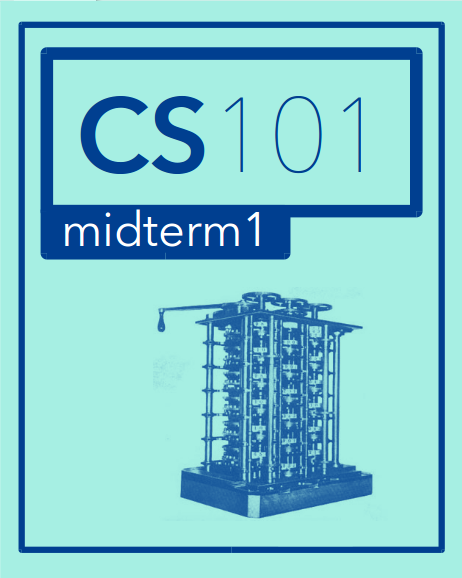
\includegraphics[width=2in]{../img/midterm1-header.png}
\end{center}

\bigskip
\noindent
\begin{itemize}
\item \textbf{Be sure to enter your \underline{NetID} and \underline{the code below} on your Scantron}.
\item Do not turn this page until instructed to do so.
\item There are 30 questions, worth 1 point each.
\item Each question has only \textbf{one} correct answer.
\item You must not communicate with other students during this test.
\item No books, notes, or electronic devices are permitted.
\item This is a 60-minute exam.
\item There are several different versions of this exam.
\end{itemize}

\bigskip\bigskip
\noindent
\textbf{\Large 1. Fill in your information:}

\bigskip
{\Large\bf
\begin{tabular}{ll}
Full Name: & \underbar{\hskip 8cm} \\[0.5em]
UIN (Student Number): & \underbar{\hskip 8cm} \\[0.5em]
NetID: & \underbar{\hskip 8cm}
\end{tabular}
}

\bigskip
\bigskip
\noindent
\textbf{\Large 2. Fill in the following answers on the Scantron form:}

%%%%%%%%%%%%%%%%%%%%%%%%%%%%%%%%%%%%%%%%%%%%%%%%%%%%%%%%%
%%%%%%%%%%%%%%%%%%%%%%%%%%%%%%%%%%%%%%%%%%%%%%%%%%%%%%%%%

\begin{enumerate}
\item[92.] B
\item[93.] D
\item[94.] A
\item[95.] C
\item[96.] E
\end{enumerate}

\newpage

% Zone 1


%%%%%%%%%%%%%%%%%%%%%%%%%%%%%%%%%%%%%%%%%%%%%%%%%%%%%%%%%



\newpage
\noindent
1. (1 point)
Evaluate the following expression:
\begin{verbatim}
len("ABCD"[0:3])
\end{verbatim}
What value is produced?


\begin{enumerate}
\item[(A)]
4

\item[(B)]
2

\item[(C)]
1

\item[(D)] $\bigstar$ 
3

\end{enumerate}

\vspace*{2em}
\hrule
\vspace{2em}

\noindent {\bf Solution.} 
\vspace{2em}
\hrule height 2pt


\newpage
\noindent
2. (1 point)
Consider the following program:
\begin{verbatim}
x=0
for i in range(2,8):
    if i%3==0:
        x+=3
    elif i%2==0:
        x+=2
    else:
        x+=1
\end{verbatim}
What is the \textbf{value} of \texttt{x} after this program is executed?


\begin{enumerate}
\item[(A)]
\begin{verbatim}11\end{verbatim}

\item[(B)]
\begin{verbatim}14\end{verbatim}

\item[(C)] $\bigstar$ 
\begin{verbatim}12\end{verbatim}

\item[(D)]
\begin{verbatim}10\end{verbatim}

\item[(E)]
\begin{verbatim}13\end{verbatim}

\end{enumerate}

\vspace*{2em}
\hrule
\vspace{2em}

\noindent {\bf Solution.} 
\vspace{2em}
\hrule height 2pt


\newpage
\noindent
3. (1 point)
Consider the following program:
\begin{verbatim}
s="TRIS %i"
t="ISEU"
x=s % len(t)
\end{verbatim}
What is the \textbf{type} of \texttt{x} after this program is executed?


\begin{enumerate}
\item[(A)]
\begin{verbatim}Float\end{verbatim}

\item[(B)]
\begin{verbatim}None\end{verbatim}

\item[(C)]
\begin{verbatim}Integer\end{verbatim}

\item[(D)]
\begin{verbatim}Boolean\end{verbatim}

\item[(E)] $\bigstar$ 
\begin{verbatim}String\end{verbatim}

\end{enumerate}

\vspace*{2em}
\hrule
\vspace{2em}

\noindent {\bf Solution.} 
\vspace{2em}
\hrule height 2pt


\newpage
\noindent
4. (1 point)
Consider the following program:
\begin{verbatim}
x=[1,2,3]
def f(a):
    s=""
    a.reverse()
    for i in a:
        s+=str(i)
    return s

x.append(f(x))
\end{verbatim}
What is the \textbf{value} of \texttt{x} after this program is executed?


\begin{enumerate}
\item[(A)]
\begin{verbatim}[3, 2, 1]\end{verbatim}

\item[(B)] $\bigstar$ 
\begin{verbatim}[3, 2, 1, '321']\end{verbatim}

\item[(C)]
\begin{verbatim}[1, 2, 3, 6]\end{verbatim}

\item[(D)]
\begin{verbatim}[1, 2, 3]\end{verbatim}

\item[(E)]
\begin{verbatim}[1, 2, 3, '321']\end{verbatim}

\end{enumerate}

\vspace*{2em}
\hrule
\vspace{2em}

\noindent {\bf Solution.} 
\vspace{2em}
\hrule height 2pt


\newpage
\noindent
5. (1 point)
Consider the following program.
\begin{verbatim}
def artificing(s):
    return s+"%i" % 2
    return s*2
    return s

s=artificing("MERLIN")
\end{verbatim}
After it is run, what is the final \textbf{value} of s?


\begin{enumerate}
\item[(A)]
\begin{verbatim}0\end{verbatim}

\item[(B)] $\bigstar$ 
\begin{verbatim}"MERLIN2"\end{verbatim}

\item[(C)]
\begin{verbatim}"MERLINMERLIN"\end{verbatim}

\item[(D)]
\begin{verbatim}None\end{verbatim}

\item[(E)]
\begin{verbatim}"MERLIN%i"\end{verbatim}

\end{enumerate}

\vspace*{2em}
\hrule
\vspace{2em}

\noindent {\bf Solution.} 
\vspace{2em}
\hrule height 2pt


\newpage
\noindent
6. (1 point)
Consider the following program:
\begin{verbatim}
x=[1,2,3,4,5,6,7,8,9]
x=x[2:-2]
i=1
while i <= 3:
    x[i]+=1
    i+=1
\end{verbatim}
What is the \textbf{value} of \texttt{x} after this program is executed?


\begin{enumerate}
\item[(A)]
\begin{verbatim}[2, 4, 5, 6, 7, 7]\end{verbatim}

\item[(B)]
\begin{verbatim}[3, 5, 6, 7, 7, 8]\end{verbatim}

\item[(C)]
\begin{verbatim}[2, 4, 5, 5, 7, 7]\end{verbatim}

\item[(D)] $\bigstar$ 
\begin{verbatim}[3, 5, 6, 7, 7]\end{verbatim}

\item[(E)]
\begin{verbatim}[3, 5, 7, 7]\end{verbatim}

\end{enumerate}

\vspace*{2em}
\hrule
\vspace{2em}

\noindent {\bf Solution.} 
\vspace{2em}
\hrule height 2pt


\newpage
\noindent
7. (1 point)
Consider the following program:
\begin{verbatim}
x=2
a=6
if (a%3)==2:
    x=x**3
elif(a%3)==1:
    x=x**2
else:
    x=x**1
\end{verbatim}
What is the \textbf{value} of \texttt{x} after this program is executed?


\begin{enumerate}
\item[(A)] $\bigstar$ 
\begin{verbatim}2\end{verbatim}

\item[(B)]
None of the other answers are correct.

\item[(C)]
\begin{verbatim}8\end{verbatim}

\item[(D)]
\begin{verbatim}16\end{verbatim}

\item[(E)]
\begin{verbatim}4\end{verbatim}

\end{enumerate}

\vspace*{2em}
\hrule
\vspace{2em}

\noindent {\bf Solution.} 
\vspace{2em}
\hrule height 2pt


\newpage
\noindent
8. (1 point)
Consider the following program:
\begin{verbatim}
s="-B-O-R-S-"
x=s.split("-")[2:-2]
\end{verbatim}
What is the \textbf{value} of \texttt{x} after this program is executed?


\begin{enumerate}
\item[(A)]
\begin{verbatim}None\end{verbatim}

\item[(B)] $\bigstar$ 
\begin{verbatim}['O', 'R']\end{verbatim}

\item[(C)]
\begin{verbatim}False\end{verbatim}

\item[(D)]
\begin{verbatim}''\end{verbatim}

\item[(E)]
\begin{verbatim}'ORS'\end{verbatim}

\end{enumerate}

\vspace*{2em}
\hrule
\vspace{2em}

\noindent {\bf Solution.} 
\vspace{2em}
\hrule height 2pt


\newpage
\noindent
9. (1 point)
What is the result of the following expression?
\begin{verbatim}
[ 1, 2, 3 ] * 3.0
\end{verbatim}


\begin{enumerate}
\item[(A)]
\begin{verbatim}[3.0, 6.0, 9.0]\end{verbatim}

\item[(B)]
\begin{verbatim}[3, 6, 9]\end{verbatim}

\item[(C)]
\begin{verbatim}[1.0, 2.0, 3.0, 1.0, 2.0, 3.0, 1.0, 2.0, 3.0]\end{verbatim}

\item[(D)]
\begin{verbatim}None of the above.\end{verbatim}

\item[(E)] $\bigstar$ 
\begin{verbatim}[1, 2, 3, 1, 2, 3, 1, 2, 3]\end{verbatim}

\end{enumerate}

\vspace*{2em}
\hrule
\vspace{2em}

\noindent {\bf Solution.} 
\vspace{2em}
\hrule height 2pt


\newpage
\noindent
10. (1 point)
Consider the following program:
\begin{verbatim}
x="KING ARTHUR-MORGANA LEFAY-SIR BEDIVERE".split("-")
y=x
x=y.reverse()
\end{verbatim}
What is the \textbf{value} of \texttt{x} after this program is executed?


\begin{enumerate}
\item[(A)]
\begin{verbatim}['KING', 'ARTHUR-MORGANA', 'LEFAY-SIR', 'BEDIVERE']\end{verbatim}

\item[(B)]
\begin{verbatim}['KING ARTHUR', 'MORGANA LEFAY', 'SIR BEDIVERE']\end{verbatim}

\item[(C)] $\bigstar$ 
\begin{verbatim}None\end{verbatim}

\item[(D)]
\begin{verbatim}['SIR BEDIVERE', 'MORGANA LEFAY', 'KING ARTHUR']\end{verbatim}

\item[(E)]
\begin{verbatim}['BEDIVERE', 'LEFAY-SIR', 'ARTHUR-MORGANA', 'KING']\end{verbatim}

\end{enumerate}

\vspace*{2em}
\hrule
\vspace{2em}

\noindent {\bf Solution.} 
\vspace{2em}
\hrule height 2pt


\newpage
\noindent
11. (1 point)
Consider the following program:
\begin{verbatim}
a=["merlin","sir agravaine","king pellinore"]
b=[ ]
for i in range(1,3):
    b.append(a[0-i].title())
\end{verbatim}
What is the \textbf{value} of b after this program is executed?


\begin{enumerate}
\item[(A)] $\bigstar$ 
\begin{verbatim}['King Pellinore', 'Sir Agravaine']\end{verbatim}

\item[(B)]
\begin{verbatim}[ ]\end{verbatim}

\item[(C)]
\begin{verbatim}['King Pellinore', 'Sir Agravaine', 'Merlin']\end{verbatim}

\item[(D)]
\begin{verbatim}['Merlin', 'King Pellinore', 'Sir Agravaine']\end{verbatim}

\item[(E)]
\begin{verbatim}['Sir Agravaine', 'King Pellinore']\end{verbatim}

\end{enumerate}

\vspace*{2em}
\hrule
\vspace{2em}

\noindent {\bf Solution.} 
\vspace{2em}
\hrule height 2pt


\newpage
\noindent
12. (1 point)
Consider the following program.
\begin{verbatim}
x=0
i=1
while(i*i)<=9:
    x=x+(i*i)
    i=i+1
\end{verbatim}
After it is run, what is the final \textbf{value} of \texttt{x}?


\begin{enumerate}
\item[(A)]
\begin{verbatim}5\end{verbatim}

\item[(B)]
\begin{verbatim}4\end{verbatim}

\item[(C)] $\bigstar$ 
\begin{verbatim}14\end{verbatim}

\item[(D)]
\begin{verbatim}30\end{verbatim}

\item[(E)]
\begin{verbatim}3\end{verbatim}

\end{enumerate}

\vspace*{2em}
\hrule
\vspace{2em}

\noindent {\bf Solution.} 
\vspace{2em}
\hrule height 2pt


\newpage
\noindent
13. (1 point)
Consider the following program:
\begin{verbatim}
x=str(1.2)*2
\end{verbatim}
What is the \textbf{value} of \texttt{x} after this program is executed?


\begin{enumerate}
\item[(A)]
\begin{verbatim}"1.2*2"\end{verbatim}

\item[(B)]
\begin{verbatim}"2.4"\end{verbatim}

\item[(C)]
None of the other answers are correct.

\item[(D)] $\bigstar$ 
\begin{verbatim}"1.21.2"\end{verbatim}

\item[(E)]
\begin{verbatim}2.4\end{verbatim}

\end{enumerate}

\vspace*{2em}
\hrule
\vspace{2em}

\noindent {\bf Solution.} 
\vspace{2em}
\hrule height 2pt


\newpage
\noindent
14. (1 point)
Consider the following program:
\begin{verbatim}
pi="3.14159"
e="2.71828"
x=pi in pi*len(e)
\end{verbatim}
What is the \textbf{type} of \texttt{x} after this program is executed?


\begin{enumerate}
\item[(A)]
\begin{verbatim}None\end{verbatim}

\item[(B)] $\bigstar$ 
\begin{verbatim}Boolean\end{verbatim}

\item[(C)]
\begin{verbatim}Float\end{verbatim}

\item[(D)]
\begin{verbatim}String\end{verbatim}

\item[(E)]
\begin{verbatim}Integer\end{verbatim}

\end{enumerate}

\vspace*{2em}
\hrule
\vspace{2em}

\noindent {\bf Solution.} 
\vspace{2em}
\hrule height 2pt


\newpage
\noindent
15. (1 point)
Consider the following program:
\begin{verbatim}
s="Hobbes"
i=0
x=-1
while i<len(s):
    if s[i]=='b':
        x=i
    i+=1
\end{verbatim}
What is the \textbf{value} of \texttt{x} after this program is executed?


\begin{enumerate}
\item[(A)]
\begin{verbatim}2\end{verbatim}

\item[(B)]
\begin{verbatim}4\end{verbatim}

\item[(C)]
\begin{verbatim}5\end{verbatim}

\item[(D)] $\bigstar$ 
\begin{verbatim}3\end{verbatim}

\item[(E)]
\begin{verbatim}-1\end{verbatim}

\end{enumerate}

\vspace*{2em}
\hrule
\vspace{2em}

\noindent {\bf Solution.} 
\vspace{2em}
\hrule height 2pt


\newpage
\noindent
16. (1 point)
Consider the following incomplete program.
\begin{verbatim}
sum=0
???:
    sum=sum+i

\end{verbatim}
The program is intended to sum all of the integers between 1 and 100 (inclusive). What should replace the three question marks to complete the program?


\begin{enumerate}
\item[(A)]
\begin{verbatim}while i<=100 \end{verbatim}

\item[(B)]
\begin{verbatim}while i in range(100)\end{verbatim}

\item[(C)]
\begin{verbatim}for i in range(0,100)\end{verbatim}

\item[(D)] $\bigstar$ 
\begin{verbatim}for i in range(1,101) \end{verbatim}

\end{enumerate}

\vspace*{2em}
\hrule
\vspace{2em}

\noindent {\bf Solution.} 
\vspace{2em}
\hrule height 2pt


\newpage
\noindent
17. (1 point)
Consider the following program:
\begin{verbatim}
def fix(s):
    a=list(s)
    a.sort()
    return ''.join(a)

x=["one","two","eleven","twelve"]
s1=fix(x[0]+x[-1])
s2=fix(x[1]+x[-2])

if s1<s2:
    x.sort()
elif s1==s2:
    x.reverse()
else:
    x.append("six")
\end{verbatim}
What is the \textbf{value} of \texttt{x} after this program is executed?


\begin{enumerate}
\item[(A)]
\begin{verbatim}['one', 'two', 'eleven', 'twelve', 'six']\end{verbatim}

\item[(B)]
\begin{verbatim}['two', 'twelve', 'one', 'eleven', 'six']\end{verbatim}

\item[(C)]
\begin{verbatim}['one', 'two', 'eleven', 'twelve']\end{verbatim}

\item[(D)]
\begin{verbatim}['eleven', 'one', 'twelve', 'two']\end{verbatim}

\item[(E)] $\bigstar$ 
\begin{verbatim}['twelve', 'eleven', 'two', 'one']\end{verbatim}

\end{enumerate}

\vspace*{2em}
\hrule
\vspace{2em}

\noindent {\bf Solution.} 
\vspace{2em}
\hrule height 2pt


\newpage
\noindent
18. (1 point)
Consider the following program.
\begin{verbatim}
kay = 2
wart = 3

def knight(kay,wart):
    wart += 2
    kay += 3
    return wart + kay

kay = knight(wart, kay) + knight(kay, wart)
\end{verbatim}
After it is run, what is the final \textbf{value} of \texttt{kay}?


\begin{enumerate}
\item[(A)]
\begin{verbatim}3\end{verbatim}

\item[(B)] $\bigstar$ 
None of the other answers are correct.

\item[(C)]
\begin{verbatim}5\end{verbatim}

\item[(D)]
\begin{verbatim}2\end{verbatim}

\end{enumerate}

\vspace*{2em}
\hrule
\vspace{2em}

\noindent {\bf Solution.} 
\vspace{2em}
\hrule height 2pt


\newpage
\noindent
19. (1 point)
Consider the following program.
\begin{verbatim}
x=[]
for j in range(0,5):
    if (j%3)==0:
        x.append("-")
    if (j%4)==0:
        x.append("*")
\end{verbatim}
After it is run, what is the final \textbf{value} of \texttt{x}?


\begin{enumerate}
\item[(A)] $\bigstar$ 
\begin{verbatim}["-","*","-","*"]\end{verbatim}

\item[(B)]
\begin{verbatim}["-","*"]\end{verbatim}

\item[(C)]
\begin{verbatim}["*","-","*"]\end{verbatim}

\item[(D)]
None of the other answers are correct.

\item[(E)]
\begin{verbatim}["*","-","*"]\end{verbatim}

\end{enumerate}

\vspace*{2em}
\hrule
\vspace{2em}

\noindent {\bf Solution.} 
\vspace{2em}
\hrule height 2pt


\newpage
\noindent
20. (1 point)
Consider the following program:
\begin{verbatim}
i=3
x=2
while i < 7:
    x+=i
    i+=2
\end{verbatim}
What is the \textbf{value} of \texttt{x} after this program is executed?


\begin{enumerate}
\item[(A)]
\begin{verbatim}14\end{verbatim}

\item[(B)]
\begin{verbatim}13\end{verbatim}

\item[(C)] $\bigstar$ 
\begin{verbatim}10\end{verbatim}

\item[(D)]
\begin{verbatim}11\end{verbatim}

\item[(E)]
\begin{verbatim}12\end{verbatim}

\end{enumerate}

\vspace*{2em}
\hrule
\vspace{2em}

\noindent {\bf Solution.} 
\vspace{2em}
\hrule height 2pt


\newpage
\noindent
21. (1 point)
Consider the following program.
\begin{verbatim}
s="BBCAA"
x=0
y=len(s)-1
while s[x]!=s[y] and x<len(s):
    x+=1
    y-=1
\end{verbatim}
After it is run, what is the final \textbf{value} of \texttt{x}?


\begin{enumerate}
\item[(A)]
\begin{verbatim}4\end{verbatim}

\item[(B)]
\begin{verbatim}3\end{verbatim}

\item[(C)] $\bigstar$ 
\begin{verbatim}2\end{verbatim}

\item[(D)]
\begin{verbatim}0\end{verbatim}

\item[(E)]
\begin{verbatim}1\end{verbatim}

\end{enumerate}

\vspace*{2em}
\hrule
\vspace{2em}

\noindent {\bf Solution.} 
\vspace{2em}
\hrule height 2pt


\newpage
\noindent
22. (1 point)
Consider the following Python program.
\begin{verbatim}
e=[1,3,5,7,9,11]
d=[0,0,0]
for i in range(0,len(e)):
    d[i%3]+=e[i]
x=d[1]
\end{verbatim}
After it is run, what is the final \textbf{value} of \texttt{x}?


\begin{enumerate}
\item[(A)]
\begin{verbatim}0\end{verbatim}

\item[(B)]
\begin{verbatim}16\end{verbatim}

\item[(C)]
\begin{verbatim}3\end{verbatim}

\item[(D)]
\begin{verbatim}8\end{verbatim}

\item[(E)] $\bigstar$ 
\begin{verbatim}12\end{verbatim}

\end{enumerate}

\vspace*{2em}
\hrule
\vspace{2em}

\noindent {\bf Solution.} 
\vspace{2em}
\hrule height 2pt


\newpage
\noindent
23. (1 point)
For this problem, you should compose a function which accomplishes a given task using the available code blocks arranged in the correct functional order.  \emph{We ignore indentation for this problem.}

\texttt{find\_max} should accept a \texttt{list} and return the value of the maximum item in the \texttt{list}.  (\texttt{None} is always the lowest value in any numeric comparison, so you may use it as an initializer.)

\begin{verbatim}
def find_max(my_list):
\end{verbatim}

\begin{enumerate}[1]
\item \texttt{max\_val = i}
\item \texttt{max\_val = None}
\item \texttt{for i in range(len(my\_list)):}
\item \texttt{if i > max\_val:}
\item \texttt{max\_val = my\_list[i]}
\item \texttt{return max\_val}
\item \texttt{for i in range(my\_list):}
\item \texttt{if my\_list[i] > max\_val:}
\item \texttt{print(max\_val)}
\end{enumerate}



\begin{enumerate}
\item[(A)]
2, 7, 4, 5, 6

\item[(B)]
2, 3, 8, 1, 6

\item[(C)]
2, 3, 4, 1, 6

\item[(D)]
3, 2, 8, 5, 9

\item[(E)] $\bigstar$ 
2, 3, 8, 5, 6

\end{enumerate}

\vspace*{2em}
\hrule
\vspace{2em}

\noindent {\bf Solution.} 
\vspace{2em}
\hrule height 2pt


\newpage
\noindent
24. (1 point)
Consider the following program:
\begin{verbatim}
a=["S","T","U","P","E","F","Y"]
a=a[0:4]
a.sort()
x=""
for e in a:
    x=e+x
\end{verbatim}
What is the \textbf{value} of \texttt{x} after this program is executed?


\begin{enumerate}
\item[(A)]
\begin{verbatim}"PUST"\end{verbatim}

\item[(B)]
\begin{verbatim}"STUP"\end{verbatim}

\item[(C)]
None of the other answers are correct.

\item[(D)] $\bigstar$ 
\begin{verbatim}"UTSP"\end{verbatim}

\item[(E)]
\begin{verbatim}"PSTU"\end{verbatim}

\end{enumerate}

\vspace*{2em}
\hrule
\vspace{2em}

\noindent {\bf Solution.} 
\vspace{2em}
\hrule height 2pt


\newpage
\noindent
25. (1 point)
Evaluate the following expression:
\begin{verbatim}
[1,2]*len("3")
\end{verbatim}
What value is produced?


\begin{enumerate}
\item[(A)] $\bigstar$ 
\begin{verbatim}[1,2]\end{verbatim}

\item[(B)]
\begin{verbatim}[1,2,3]\end{verbatim}

\item[(C)]
\begin{verbatim}[1,2,1,2,1,2]\end{verbatim}

\item[(D)]
\begin{verbatim}[1,2,1]\end{verbatim}

\end{enumerate}

\vspace*{2em}
\hrule
\vspace{2em}

\noindent {\bf Solution.} 
\vspace{2em}
\hrule height 2pt


\newpage
\noindent
26. (1 point)
How can the following mathematical equation be implemented as a Python expression? Assume \verb|a|, \verb|b|, and \verb|sin| have already been defined.
$$a \sin(a^b - b)$$


\begin{enumerate}
\item[(A)]
\begin{verbatim}a*sin(b^a - b)\end{verbatim}

\item[(B)]
\begin{verbatim}a*sin(a^b - b)\end{verbatim}

\item[(C)]
\begin{verbatim}a sin(a**b - b)\end{verbatim}

\item[(D)]
None of the other answers are correct.

\item[(E)] $\bigstar$ 
\begin{verbatim}a*sin(a**b - b)\end{verbatim}

\end{enumerate}

\vspace*{2em}
\hrule
\vspace{2em}

\noindent {\bf Solution.} 
\vspace{2em}
\hrule height 2pt


\newpage
\noindent
27. (1 point)
Consider the following program:
\begin{verbatim}
a=3
b=4
if a!=b:
    a=b
elif a==4:
    a=5
else:
    b=a
\end{verbatim}
What is the \textbf{value} of a after this program is executed?


\begin{enumerate}
\item[(A)]
None of the other answers are correct.

\item[(B)] $\bigstar$ 
\begin{verbatim}4\end{verbatim}

\item[(C)]
\begin{verbatim}5\end{verbatim}

\item[(D)]
\begin{verbatim}3\end{verbatim}

\item[(E)]
\begin{verbatim}7\end{verbatim}

\end{enumerate}

\vspace*{2em}
\hrule
\vspace{2em}

\noindent {\bf Solution.} 
\vspace{2em}
\hrule height 2pt


\newpage
\noindent
28. (1 point)
Consider the following program:
\begin{verbatim}
s="ECTOR"
t="GAWAIN"
x=(len(s)/(len(t)-1))+1
\end{verbatim}
What is the \textbf{type} of \texttt{x} after this program is executed?


\begin{enumerate}
\item[(A)]
\begin{verbatim}String\end{verbatim}

\item[(B)] $\bigstar$ 
\begin{verbatim}Float\end{verbatim}

\item[(C)]
\begin{verbatim}None\end{verbatim}

\item[(D)]
\begin{verbatim}Integer\end{verbatim}

\item[(E)]
\begin{verbatim}Boolean\end{verbatim}

\end{enumerate}

\vspace*{2em}
\hrule
\vspace{2em}

\noindent {\bf Solution.} 
\vspace{2em}
\hrule height 2pt


\newpage
\noindent
29. (1 point)
Consider the following incomplete Python program.
\begin{verbatim}
s="".join(["1","0","2","1"])
x=0
for i in range(len(s)-1):
    x+=int(???)
\end{verbatim}
What should replace the three question marks so the resulting value of \texttt{x} is 33?


\begin{enumerate}
\item[(A)] $\bigstar$ 
\begin{verbatim}s[i:i+2]\end{verbatim}

\item[(B)]
\begin{verbatim}s[i:i+1]\end{verbatim}

\item[(C)]
\begin{verbatim}s[i+1:i+2]\end{verbatim}

\item[(D)]
\begin{verbatim}s[i:i-1]\end{verbatim}

\end{enumerate}

\vspace*{2em}
\hrule
\vspace{2em}

\noindent {\bf Solution.} 
\vspace{2em}
\hrule height 2pt


\newpage
\noindent
30. (1 point)
Consider the following incomplete function.
\begin{verbatim}
def ismultiple(m,n):
    if ???:
        return False
    else:
        return True
\end{verbatim}
The function is intended to return True if the input parameter m is a multiple of parameter n and False otherwise. For example, \verb|ismultiple(4,2)| should return \verb|True|, but \verb|ismultiple(5,3)| should return \verb|False|. What should replace the three question marks to complete the function?


\begin{enumerate}
\item[(A)]
\begin{verbatim}(m // n) != 0 \end{verbatim}

\item[(B)]
\begin{verbatim}(n // m) == 0 \end{verbatim}

\item[(C)]
\begin{verbatim}(n % m) == 0 \end{verbatim}

\item[(D)] $\bigstar$ 
\begin{verbatim}(m % n) != 0 \end{verbatim}

\end{enumerate}

\vspace*{2em}
\hrule
\vspace{2em}

\noindent {\bf Solution.} 
\vspace{2em}
\hrule height 2pt

%%%%%%%%%%%%%%%%%%%%%%%%%%%%%%%%%%%%%%%%%%%%%%%%%%%%%%%%%%%%%%%%%%%%%%
%%%%%%%%%%%%%%%%%%%%%%%%%%%%%%%%%%%%%%%%%%%%%%%%%%%%%%%%%%%%%%%%%%%%%%
%%%%%%%%%%%%%%%%%%%%%%%%%%%%%%%%%%%%%%%%%%%%%%%%%%%%%%%%%%%%%%%%%%%%%%
%%%%%%%%%%%%%%%%%%%%%%%%%%%%%%%%%%%%%%%%%%%%%%%%%%%%%%%%%%%%%%%%%%%%%%
% Exam number 18

\message{Exam 18/50}
\cleardoublepage
\setcounter{page}{1}


\begin{center}
%\textbf{\Large CS 101 Midterm \#1}
%
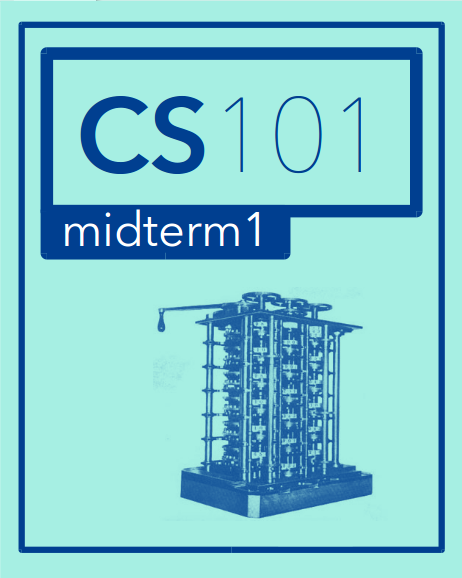
\includegraphics[width=2in]{../img/midterm1-header.png}
\end{center}

\bigskip
\noindent
\begin{itemize}
\item \textbf{Be sure to enter your \underline{NetID} and \underline{the code below} on your Scantron}.
\item Do not turn this page until instructed to do so.
\item There are 30 questions, worth 1 point each.
\item Each question has only \textbf{one} correct answer.
\item You must not communicate with other students during this test.
\item No books, notes, or electronic devices are permitted.
\item This is a 60-minute exam.
\item There are several different versions of this exam.
\end{itemize}

\bigskip\bigskip
\noindent
\textbf{\Large 1. Fill in your information:}

\bigskip
{\Large\bf
\begin{tabular}{ll}
Full Name: & \underbar{\hskip 8cm} \\[0.5em]
UIN (Student Number): & \underbar{\hskip 8cm} \\[0.5em]
NetID: & \underbar{\hskip 8cm}
\end{tabular}
}

\bigskip
\bigskip
\noindent
\textbf{\Large 2. Fill in the following answers on the Scantron form:}

%%%%%%%%%%%%%%%%%%%%%%%%%%%%%%%%%%%%%%%%%%%%%%%%%%%%%%%%%
%%%%%%%%%%%%%%%%%%%%%%%%%%%%%%%%%%%%%%%%%%%%%%%%%%%%%%%%%

\begin{enumerate}
\item[92.] C
\item[93.] D
\item[94.] A
\item[95.] D
\item[96.] A
\end{enumerate}

\newpage

% Zone 1


%%%%%%%%%%%%%%%%%%%%%%%%%%%%%%%%%%%%%%%%%%%%%%%%%%%%%%%%%



\newpage
\noindent
1. (1 point)
Consider the following program:
\begin{verbatim}
i=2
x=3
while i < 7:
    x+=i
    i+=2
\end{verbatim}
What is the \textbf{value} of \texttt{x} after this program is executed?


\begin{enumerate}
\item[(A)]
\begin{verbatim}11\end{verbatim}

\item[(B)]
\begin{verbatim}12\end{verbatim}

\item[(C)]
\begin{verbatim}13\end{verbatim}

\item[(D)]
\begin{verbatim}14\end{verbatim}

\item[(E)] $\bigstar$ 
\begin{verbatim}15\end{verbatim}

\end{enumerate}

\vspace*{2em}
\hrule
\vspace{2em}

\noindent {\bf Solution.} 
\vspace{2em}
\hrule height 2pt


\newpage
\noindent
2. (1 point)
What is the result of the following expression?
\begin{verbatim}
[ 1, 2, 3 ] * 3
\end{verbatim}


\begin{enumerate}
\item[(A)] $\bigstar$ 
\begin{verbatim}[1, 2, 3, 1, 2, 3, 1, 2, 3]\end{verbatim}

\item[(B)]
\begin{verbatim}[3, 6, 9]\end{verbatim}

\item[(C)]
\begin{verbatim}(3, 6, 9)\end{verbatim}

\item[(D)]
\begin{verbatim}[3.0, 6.0, 9.0]\end{verbatim}

\item[(E)]
\begin{verbatim}[1.0, 2.0, 3.0, 1.0, 2.0, 3.0, 1.0, 2.0, 3.0]\end{verbatim}

\end{enumerate}

\vspace*{2em}
\hrule
\vspace{2em}

\noindent {\bf Solution.} 
\vspace{2em}
\hrule height 2pt


\newpage
\noindent
3. (1 point)
Consider the following program:
\begin{verbatim}
x=[1,2,3]
def f(a):
    s=""
    a.reverse()
    for i in a:
        s+=str(i)
    return s

x.append(f(x))
\end{verbatim}
What is the \textbf{value} of \texttt{x} after this program is executed?


\begin{enumerate}
\item[(A)]
\begin{verbatim}[1, 2, 3, '321']\end{verbatim}

\item[(B)]
\begin{verbatim}[1, 2, 3]\end{verbatim}

\item[(C)]
\begin{verbatim}[3, 2, 1]\end{verbatim}

\item[(D)] $\bigstar$ 
\begin{verbatim}[3, 2, 1, '321']\end{verbatim}

\item[(E)]
\begin{verbatim}[1, 2, 3, 6]\end{verbatim}

\end{enumerate}

\vspace*{2em}
\hrule
\vspace{2em}

\noindent {\bf Solution.} 
\vspace{2em}
\hrule height 2pt


\newpage
\noindent
4. (1 point)
Consider the following program:
\begin{verbatim}
s="ECTOR"
t="GAWAIN"
x=(len(s)/(len(t)-1))+1
\end{verbatim}
What is the \textbf{type} of \texttt{x} after this program is executed?


\begin{enumerate}
\item[(A)]
\begin{verbatim}String\end{verbatim}

\item[(B)]
\begin{verbatim}None\end{verbatim}

\item[(C)] $\bigstar$ 
\begin{verbatim}Float\end{verbatim}

\item[(D)]
\begin{verbatim}Integer\end{verbatim}

\item[(E)]
\begin{verbatim}Boolean\end{verbatim}

\end{enumerate}

\vspace*{2em}
\hrule
\vspace{2em}

\noindent {\bf Solution.} 
\vspace{2em}
\hrule height 2pt


\newpage
\noindent
5. (1 point)
Consider the following program:
\begin{verbatim}
x="KING ARTHUR-MORGANA LEFAY-SIR BEDIVERE".split("-")
y=x
y.reverse()
\end{verbatim}
What is the \textbf{value} of \texttt{x} after this program is executed?


\begin{enumerate}
\item[(A)] $\bigstar$ 
\begin{verbatim}['SIR BEDIVERE', 'MORGANA LEFAY', 'KING ARTHUR']\end{verbatim}

\item[(B)]
\begin{verbatim}['KING ARTHUR', 'MORGANA LEFAY', 'SIR BEDIVERE']\end{verbatim}

\item[(C)]
\begin{verbatim}['KING', 'ARTHUR-MORGANA', 'LEFAY-SIR', 'BEDIVERE']\end{verbatim}

\item[(D)]
\begin{verbatim}['BEDIVERE', 'LEFAY-SIR', 'ARTHUR-MORGANA', 'KING']\end{verbatim}

\item[(E)]
\begin{verbatim}None\end{verbatim}

\end{enumerate}

\vspace*{2em}
\hrule
\vspace{2em}

\noindent {\bf Solution.} 
\vspace{2em}
\hrule height 2pt


\newpage
\noindent
6. (1 point)
How can the following mathematical equation be implemented as a Python expression? Assume \verb|a|, \verb|b|, and \verb|sin| have already been defined.
$$a \sin(a^b - b)$$


\begin{enumerate}
\item[(A)]
\begin{verbatim}a*sin(b^a - b)\end{verbatim}

\item[(B)]
\begin{verbatim}a*sin(a^b - b)\end{verbatim}

\item[(C)] $\bigstar$ 
\begin{verbatim}a*sin(a**b - b)\end{verbatim}

\item[(D)]
None of the other answers are correct.

\item[(E)]
\begin{verbatim}a sin(a**b - b)\end{verbatim}

\end{enumerate}

\vspace*{2em}
\hrule
\vspace{2em}

\noindent {\bf Solution.} 
\vspace{2em}
\hrule height 2pt


\newpage
\noindent
7. (1 point)
Consider the following program:
\begin{verbatim}
a=["merlin","sir agravaine","king pellinore"]
b=[ ]
for i in range(0,4):
    b.append(a[0-i].title())
\end{verbatim}
What is the \textbf{value} of b after this program is executed?


\begin{enumerate}
\item[(A)]
\begin{verbatim}['King Pellinore', 'Sir Agravaine', 'Merlin']\end{verbatim}

\item[(B)] $\bigstar$ 
\begin{verbatim}['Merlin', 'King Pellinore', 'Sir Agravaine', 'Merlin']\end{verbatim}

\item[(C)]
\begin{verbatim}['Merlin', 'Sir Agravaine', 'King Pellinore', 'Merlin']\end{verbatim}

\item[(D)]
\begin{verbatim}[ ]\end{verbatim}

\item[(E)]
\begin{verbatim}['Merlin', 'King Pellinore', 'Sir Agravaine']\end{verbatim}

\end{enumerate}

\vspace*{2em}
\hrule
\vspace{2em}

\noindent {\bf Solution.} 
\vspace{2em}
\hrule height 2pt


\newpage
\noindent
8. (1 point)
Consider the following program:
\begin{verbatim}
def fix(s):
    a=list(s)
    a.sort()
    return ''.join(a)

x=["one","two","eleven","twelve"]
s1=fix(x[0]+x[-1])
s2=fix(x[1]+x[-2])

if s1<s2:
    x.sort()
elif s1==s2:
    x.reverse()
else:
    x.append("six")
\end{verbatim}
What is the \textbf{value} of \texttt{x} after this program is executed?


\begin{enumerate}
\item[(A)]
\begin{verbatim}['one', 'two', 'eleven', 'twelve', 'six']\end{verbatim}

\item[(B)]
\begin{verbatim}['eleven', 'one', 'twelve', 'two']\end{verbatim}

\item[(C)]
\begin{verbatim}['two', 'twelve', 'one', 'eleven', 'six']\end{verbatim}

\item[(D)]
\begin{verbatim}['one', 'two', 'eleven', 'twelve']\end{verbatim}

\item[(E)] $\bigstar$ 
\begin{verbatim}['twelve', 'eleven', 'two', 'one']\end{verbatim}

\end{enumerate}

\vspace*{2em}
\hrule
\vspace{2em}

\noindent {\bf Solution.} 
\vspace{2em}
\hrule height 2pt


\newpage
\noindent
9. (1 point)
Consider the following program:
\begin{verbatim}
s="Calvin"
i=0
x=-1
while i<len(s):
    if s[i]=='b':
        x=i
    i+=1
\end{verbatim}
What is the \textbf{value} of \texttt{x} after this program is executed?


\begin{enumerate}
\item[(A)]
\begin{verbatim}0\end{verbatim}

\item[(B)]
\begin{verbatim}6\end{verbatim}

\item[(C)]
\begin{verbatim}3\end{verbatim}

\item[(D)]
\begin{verbatim}5\end{verbatim}

\item[(E)] $\bigstar$ 
\begin{verbatim}-1\end{verbatim}

\end{enumerate}

\vspace*{2em}
\hrule
\vspace{2em}

\noindent {\bf Solution.} 
\vspace{2em}
\hrule height 2pt


\newpage
\noindent
10. (1 point)
Consider the following program.
\begin{verbatim}
s="ABCBA"
x=0
y=len(s)-1
while s[x]==s[y] and x<y:
    x+=1
    y-=1
\end{verbatim}
After it is run, what is the final \textbf{value} of \texttt{x}?


\begin{enumerate}
\item[(A)] $\bigstar$ 
\begin{verbatim}2\end{verbatim}

\item[(B)]
\begin{verbatim}1\end{verbatim}

\item[(C)]
\begin{verbatim}3\end{verbatim}

\item[(D)]
\begin{verbatim}4\end{verbatim}

\item[(E)]
\begin{verbatim}0\end{verbatim}

\end{enumerate}

\vspace*{2em}
\hrule
\vspace{2em}

\noindent {\bf Solution.} 
\vspace{2em}
\hrule height 2pt


\newpage
\noindent
11. (1 point)
Evaluate the following expression:
\begin{verbatim}
[1,2]+[len("3")]
\end{verbatim}
What value is produced?


\begin{enumerate}
\item[(A)]
\begin{verbatim}[1,2,1,2,1,2]\end{verbatim}

\item[(B)]
\begin{verbatim}[1,2,3]\end{verbatim}

\item[(C)] $\bigstar$ 
\begin{verbatim}[1,2,1]\end{verbatim}

\item[(D)]
\begin{verbatim}[1,2,"3"]\end{verbatim}

\end{enumerate}

\vspace*{2em}
\hrule
\vspace{2em}

\noindent {\bf Solution.} 
\vspace{2em}
\hrule height 2pt


\newpage
\noindent
12. (1 point)
Consider the following incomplete Python program.
\begin{verbatim}
s="".join(["1","0","2","1"])
x=0
for i in range(len(s)-1):
    x+=int(???)
\end{verbatim}
What should replace the three question marks so the resulting value of \texttt{x} is 33?


\begin{enumerate}
\item[(A)] $\bigstar$ 
\begin{verbatim}s[i:i+2]\end{verbatim}

\item[(B)]
\begin{verbatim}s[i+1:i+2]\end{verbatim}

\item[(C)]
\begin{verbatim}s[i:i+1]\end{verbatim}

\item[(D)]
\begin{verbatim}s[i:i-1]\end{verbatim}

\end{enumerate}

\vspace*{2em}
\hrule
\vspace{2em}

\noindent {\bf Solution.} 
\vspace{2em}
\hrule height 2pt


\newpage
\noindent
13. (1 point)
Consider the following incomplete program.
\begin{verbatim}
sum=0
???:
    sum=sum+i

\end{verbatim}
The program is intended to sum all of the integers between 1 and 100 (inclusive). What should replace the three question marks to complete the program?


\begin{enumerate}
\item[(A)]
\begin{verbatim}for i in range(0,100)\end{verbatim}

\item[(B)]
\begin{verbatim}while i<=100 \end{verbatim}

\item[(C)]
\begin{verbatim}while i in range(100)\end{verbatim}

\item[(D)] $\bigstar$ 
\begin{verbatim}for i in range(1,101) \end{verbatim}

\end{enumerate}

\vspace*{2em}
\hrule
\vspace{2em}

\noindent {\bf Solution.} 
\vspace{2em}
\hrule height 2pt


\newpage
\noindent
14. (1 point)
Consider the following incomplete function.
\begin{verbatim}
def ismultiple(m,n):
    if ???:
        return False
    else:
        return True
\end{verbatim}
The function is intended to return True if the input parameter m is a multiple of parameter n and False otherwise. For example, \verb|ismultiple(4,2)| should return \verb|True|, but \verb|ismultiple(5,3)| should return \verb|False|. What should replace the three question marks to complete the function?


\begin{enumerate}
\item[(A)]
\begin{verbatim}(n % m) == 0 \end{verbatim}

\item[(B)]
\begin{verbatim}(m // n) != 0 \end{verbatim}

\item[(C)]
\begin{verbatim}(n // m) == 0 \end{verbatim}

\item[(D)] $\bigstar$ 
\begin{verbatim}(m % n) != 0 \end{verbatim}

\end{enumerate}

\vspace*{2em}
\hrule
\vspace{2em}

\noindent {\bf Solution.} 
\vspace{2em}
\hrule height 2pt


\newpage
\noindent
15. (1 point)
Consider the following program:
\begin{verbatim}
x=[1,2,3,4,5,6,7,8,9]
x=x[2:-2]
i=1
while i <= 3:
    x[i]+=1
    i+=1
\end{verbatim}
What is the \textbf{value} of \texttt{x} after this program is executed?


\begin{enumerate}
\item[(A)]
\begin{verbatim}[2, 4, 5, 5, 7, 7]\end{verbatim}

\item[(B)] $\bigstar$ 
\begin{verbatim}[3, 5, 6, 7, 7]\end{verbatim}

\item[(C)]
\begin{verbatim}[3, 5, 6, 7, 7, 8]\end{verbatim}

\item[(D)]
\begin{verbatim}[2, 4, 5, 6, 7, 7]\end{verbatim}

\item[(E)]
\begin{verbatim}[3, 5, 7, 7]\end{verbatim}

\end{enumerate}

\vspace*{2em}
\hrule
\vspace{2em}

\noindent {\bf Solution.} 
\vspace{2em}
\hrule height 2pt


\newpage
\noindent
16. (1 point)
Evaluate the following expression:
\begin{verbatim}
len("ABCDE"[1:4])
\end{verbatim}
What value is produced?


\begin{enumerate}
\item[(A)]
5

\item[(B)] $\bigstar$ 
3

\item[(C)]
4

\item[(D)]
1

\end{enumerate}

\vspace*{2em}
\hrule
\vspace{2em}

\noindent {\bf Solution.} 
\vspace{2em}
\hrule height 2pt


\newpage
\noindent
17. (1 point)
Consider the following program.
\begin{verbatim}
kay = 2
wart = 3

def knight(kay,wart):
    wart += 2
    kay += 3
    return wart + kay

kay = knight(wart, kay) + knight(kay, wart)
\end{verbatim}
After it is run, what is the final \textbf{value} of \texttt{kay}?


\begin{enumerate}
\item[(A)] $\bigstar$ 
None of the other answers are correct.

\item[(B)]
\begin{verbatim}5\end{verbatim}

\item[(C)]
\begin{verbatim}3\end{verbatim}

\item[(D)]
\begin{verbatim}2\end{verbatim}

\end{enumerate}

\vspace*{2em}
\hrule
\vspace{2em}

\noindent {\bf Solution.} 
\vspace{2em}
\hrule height 2pt


\newpage
\noindent
18. (1 point)
Consider the following program:
\begin{verbatim}
x=2
a=6
if (a%3)==2:
    x=x**3
elif(a%3)==1:
    x=x**2
else:
    x=x**1
\end{verbatim}
What is the \textbf{value} of \texttt{x} after this program is executed?


\begin{enumerate}
\item[(A)]
None of the other answers are correct.

\item[(B)]
\begin{verbatim}8\end{verbatim}

\item[(C)]
\begin{verbatim}4\end{verbatim}

\item[(D)] $\bigstar$ 
\begin{verbatim}2\end{verbatim}

\item[(E)]
\begin{verbatim}16\end{verbatim}

\end{enumerate}

\vspace*{2em}
\hrule
\vspace{2em}

\noindent {\bf Solution.} 
\vspace{2em}
\hrule height 2pt


\newpage
\noindent
19. (1 point)
Consider the following program:
\begin{verbatim}
s="TRIS %i"
t="ISEU"
x=s % len(t)
\end{verbatim}
What is the \textbf{type} of \texttt{x} after this program is executed?


\begin{enumerate}
\item[(A)]
\begin{verbatim}Integer\end{verbatim}

\item[(B)] $\bigstar$ 
\begin{verbatim}String\end{verbatim}

\item[(C)]
\begin{verbatim}None\end{verbatim}

\item[(D)]
\begin{verbatim}Float\end{verbatim}

\item[(E)]
\begin{verbatim}Boolean\end{verbatim}

\end{enumerate}

\vspace*{2em}
\hrule
\vspace{2em}

\noindent {\bf Solution.} 
\vspace{2em}
\hrule height 2pt


\newpage
\noindent
20. (1 point)
Consider the following program.
\begin{verbatim}
x=1
i=0
while(x*x)<=9:
    i=i+(x*x)
    x=x+1
\end{verbatim}
After it is run, what is the final \textbf{value} of \texttt{x}?


\begin{enumerate}
\item[(A)]
\begin{verbatim}14\end{verbatim}

\item[(B)]
\begin{verbatim}3\end{verbatim}

\item[(C)]
\begin{verbatim}5\end{verbatim}

\item[(D)]
\begin{verbatim}30\end{verbatim}

\item[(E)] $\bigstar$ 
\begin{verbatim}4\end{verbatim}

\end{enumerate}

\vspace*{2em}
\hrule
\vspace{2em}

\noindent {\bf Solution.} 
\vspace{2em}
\hrule height 2pt


\newpage
\noindent
21. (1 point)
Consider the following program:
\begin{verbatim}
pi="3.14159"
e="2.71828"
x=pi*len(e)+pi
\end{verbatim}
What is the \textbf{type} of \texttt{x} after this program is executed?


\begin{enumerate}
\item[(A)] $\bigstar$ 
\begin{verbatim}String\end{verbatim}

\item[(B)]
\begin{verbatim}Boolean\end{verbatim}

\item[(C)]
\begin{verbatim}Float\end{verbatim}

\item[(D)]
\begin{verbatim}Integer\end{verbatim}

\item[(E)]
\begin{verbatim}None\end{verbatim}

\end{enumerate}

\vspace*{2em}
\hrule
\vspace{2em}

\noindent {\bf Solution.} 
\vspace{2em}
\hrule height 2pt


\newpage
\noindent
22. (1 point)
Consider the following program.
\begin{verbatim}
x=[]
for j in range(0,5):
    if (j%4)==0:
        x.append("-")
    if (j%5)==0:
        x.append("*")
\end{verbatim}
After it is run, what is the final \textbf{value} of \texttt{x}?


\begin{enumerate}
\item[(A)]
\begin{verbatim}["-","*"]\end{verbatim}

\item[(B)]
\begin{verbatim}["-","-","*"]\end{verbatim}

\item[(C)] $\bigstar$ 
\begin{verbatim}["-","*","-"]\end{verbatim}

\item[(D)]
\begin{verbatim}["-","*","*"]\end{verbatim}

\item[(E)]
None of the other answers are correct.

\end{enumerate}

\vspace*{2em}
\hrule
\vspace{2em}

\noindent {\bf Solution.} 
\vspace{2em}
\hrule height 2pt


\newpage
\noindent
23. (1 point)
For this problem, you should compose a function which accomplishes a given task using the available code blocks arranged in the correct functional order.  \emph{We ignore indentation for this problem.}

\texttt{find\_max} should accept a \texttt{list} and return the value of the maximum item in the \texttt{list}.  (\texttt{None} is always the lowest value in any numeric comparison, so you may use it as an initializer.)

\begin{verbatim}
def find_max(my_list):
\end{verbatim}

\begin{enumerate}[1]
\item \texttt{max\_val = i}
\item \texttt{max\_val = None}
\item \texttt{for i in range(len(my\_list)):}
\item \texttt{if i > max\_val:}
\item \texttt{max\_val = my\_list[i]}
\item \texttt{return max\_val}
\item \texttt{for i in range(my\_list):}
\item \texttt{if my\_list[i] > max\_val:}
\item \texttt{print(max\_val)}
\end{enumerate}



\begin{enumerate}
\item[(A)] $\bigstar$ 
2, 3, 8, 5, 6

\item[(B)]
2, 3, 8, 1, 6

\item[(C)]
3, 2, 8, 5, 9

\item[(D)]
2, 3, 4, 1, 6

\item[(E)]
2, 7, 4, 5, 6

\end{enumerate}

\vspace*{2em}
\hrule
\vspace{2em}

\noindent {\bf Solution.} 
\vspace{2em}
\hrule height 2pt


\newpage
\noindent
24. (1 point)
Consider the following program:
\begin{verbatim}
s="-B-O-R-S-"
x=s.split("-")[2:-2]
\end{verbatim}
What is the \textbf{value} of \texttt{x} after this program is executed?


\begin{enumerate}
\item[(A)] $\bigstar$ 
\begin{verbatim}['O', 'R']\end{verbatim}

\item[(B)]
\begin{verbatim}False\end{verbatim}

\item[(C)]
\begin{verbatim}'ORS'\end{verbatim}

\item[(D)]
\begin{verbatim}''\end{verbatim}

\item[(E)]
\begin{verbatim}None\end{verbatim}

\end{enumerate}

\vspace*{2em}
\hrule
\vspace{2em}

\noindent {\bf Solution.} 
\vspace{2em}
\hrule height 2pt


\newpage
\noindent
25. (1 point)
Consider the following program:
\begin{verbatim}
x=0
for i in range(4,10):
    if i%3==0:
        x+=3
    elif i%2==0:
        x+=2
    else:
        x+=1
\end{verbatim}
What is the \textbf{value} of \texttt{x} after this program is executed?


\begin{enumerate}
\item[(A)]
\begin{verbatim}13\end{verbatim}

\item[(B)]
\begin{verbatim}14\end{verbatim}

\item[(C)]
\begin{verbatim}10\end{verbatim}

\item[(D)] $\bigstar$ 
\begin{verbatim}12\end{verbatim}

\item[(E)]
\begin{verbatim}11\end{verbatim}

\end{enumerate}

\vspace*{2em}
\hrule
\vspace{2em}

\noindent {\bf Solution.} 
\vspace{2em}
\hrule height 2pt


\newpage
\noindent
26. (1 point)
\begin{verbatim}
x=str(3)+"str(3)"
\end{verbatim}
What is the \textbf{value} of \texttt{x} after this program is executed?


\begin{enumerate}
\item[(A)]
\begin{verbatim}33\end{verbatim}

\item[(B)] $\bigstar$ 
\begin{verbatim}"3str(3)"\end{verbatim}

\item[(C)]
None of the other answers are correct.

\item[(D)]
\begin{verbatim}"33"\end{verbatim}

\item[(E)]
\begin{verbatim}"333"\end{verbatim}

\end{enumerate}

\vspace*{2em}
\hrule
\vspace{2em}

\noindent {\bf Solution.} 
\vspace{2em}
\hrule height 2pt


\newpage
\noindent
27. (1 point)
Consider the following program:
\begin{verbatim}
a=["A","C","C","I","O"]
a.sort()
a[0]=a[-1]
x=""
for e in a:
    x=x+e
\end{verbatim}
What is the \textbf{value} of \texttt{x} after this program is executed?


\begin{enumerate}
\item[(A)]
\begin{verbatim}"ACCOA"\end{verbatim}

\item[(B)] $\bigstar$ 
\begin{verbatim}"OCCIO"\end{verbatim}

\item[(C)]
\begin{verbatim}"ACCIA"\end{verbatim}

\item[(D)]
None of the other answers are correct.

\item[(E)]
\begin{verbatim}"ICCOI"\end{verbatim}

\end{enumerate}

\vspace*{2em}
\hrule
\vspace{2em}

\noindent {\bf Solution.} 
\vspace{2em}
\hrule height 2pt


\newpage
\noindent
28. (1 point)
Consider the following program:
\begin{verbatim}
a=3
b=4
if a==3:
    b=a
elif a==4:
    a=5
else:
    a=b
\end{verbatim}
What is the \textbf{value} of a after this program is executed?


\begin{enumerate}
\item[(A)] $\bigstar$ 
\begin{verbatim}3\end{verbatim}

\item[(B)]
\begin{verbatim}4\end{verbatim}

\item[(C)]
\begin{verbatim}5\end{verbatim}

\item[(D)]
None of the other answers are correct.

\item[(E)]
\begin{verbatim}7\end{verbatim}

\end{enumerate}

\vspace*{2em}
\hrule
\vspace{2em}

\noindent {\bf Solution.} 
\vspace{2em}
\hrule height 2pt


\newpage
\noindent
29. (1 point)
Consider the following Python program.
\begin{verbatim}
e=[1,3,5,7,9,11]
d=[0,0,0]
for i in range(0,len(e)):
    d[i%3]+=e[i]
x=d[2]
\end{verbatim}
After it is run, what is the final \textbf{value} of \texttt{x}?


\begin{enumerate}
\item[(A)]
\begin{verbatim}0\end{verbatim}

\item[(B)]
\begin{verbatim}7\end{verbatim}

\item[(C)] $\bigstar$ 
\begin{verbatim}16\end{verbatim}

\item[(D)]
\begin{verbatim}8\end{verbatim}

\item[(E)]
\begin{verbatim}12\end{verbatim}

\end{enumerate}

\vspace*{2em}
\hrule
\vspace{2em}

\noindent {\bf Solution.} 
\vspace{2em}
\hrule height 2pt


\newpage
\noindent
30. (1 point)
Consider the following program.
\begin{verbatim}
def artificing(s):
    return s*2
    return s+"%i" % 2
    return s

s=artificing("MERLIN")
\end{verbatim}
After it is run, what is the final \textbf{value} of s?


\begin{enumerate}
\item[(A)]
\begin{verbatim}12\end{verbatim}

\item[(B)]
\begin{verbatim}None\end{verbatim}

\item[(C)]
\begin{verbatim}"MERLIN2"\end{verbatim}

\item[(D)] $\bigstar$ 
\begin{verbatim}"MERLINMERLIN"\end{verbatim}

\item[(E)]
\begin{verbatim}"MERLIN"\end{verbatim}

\end{enumerate}

\vspace*{2em}
\hrule
\vspace{2em}

\noindent {\bf Solution.} 
\vspace{2em}
\hrule height 2pt

%%%%%%%%%%%%%%%%%%%%%%%%%%%%%%%%%%%%%%%%%%%%%%%%%%%%%%%%%%%%%%%%%%%%%%
%%%%%%%%%%%%%%%%%%%%%%%%%%%%%%%%%%%%%%%%%%%%%%%%%%%%%%%%%%%%%%%%%%%%%%
%%%%%%%%%%%%%%%%%%%%%%%%%%%%%%%%%%%%%%%%%%%%%%%%%%%%%%%%%%%%%%%%%%%%%%
%%%%%%%%%%%%%%%%%%%%%%%%%%%%%%%%%%%%%%%%%%%%%%%%%%%%%%%%%%%%%%%%%%%%%%
% Exam number 19

\message{Exam 19/50}
\cleardoublepage
\setcounter{page}{1}


\begin{center}
%\textbf{\Large CS 101 Midterm \#1}
%
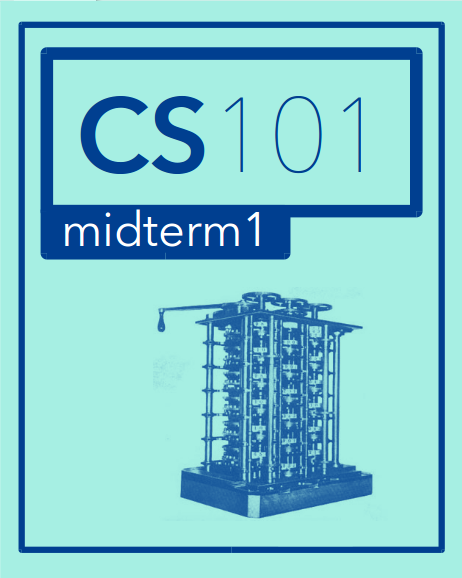
\includegraphics[width=2in]{../img/midterm1-header.png}
\end{center}

\bigskip
\noindent
\begin{itemize}
\item \textbf{Be sure to enter your \underline{NetID} and \underline{the code below} on your Scantron}.
\item Do not turn this page until instructed to do so.
\item There are 30 questions, worth 1 point each.
\item Each question has only \textbf{one} correct answer.
\item You must not communicate with other students during this test.
\item No books, notes, or electronic devices are permitted.
\item This is a 60-minute exam.
\item There are several different versions of this exam.
\end{itemize}

\bigskip\bigskip
\noindent
\textbf{\Large 1. Fill in your information:}

\bigskip
{\Large\bf
\begin{tabular}{ll}
Full Name: & \underbar{\hskip 8cm} \\[0.5em]
UIN (Student Number): & \underbar{\hskip 8cm} \\[0.5em]
NetID: & \underbar{\hskip 8cm}
\end{tabular}
}

\bigskip
\bigskip
\noindent
\textbf{\Large 2. Fill in the following answers on the Scantron form:}

%%%%%%%%%%%%%%%%%%%%%%%%%%%%%%%%%%%%%%%%%%%%%%%%%%%%%%%%%
%%%%%%%%%%%%%%%%%%%%%%%%%%%%%%%%%%%%%%%%%%%%%%%%%%%%%%%%%

\begin{enumerate}
\item[92.] D
\item[93.] D
\item[94.] A
\item[95.] E
\item[96.] B
\end{enumerate}

\newpage

% Zone 1


%%%%%%%%%%%%%%%%%%%%%%%%%%%%%%%%%%%%%%%%%%%%%%%%%%%%%%%%%



\newpage
\noindent
1. (1 point)
Consider the following program:
\begin{verbatim}
x=[2,3,4,5,6,7,8,9]
x=x[2:-2]
i=1
while i <= 3:
    x[i]+=1
    i+=1
\end{verbatim}
What is the \textbf{value} of \texttt{x} after this program is executed?


\begin{enumerate}
\item[(A)]
\begin{verbatim}[2, 4, 6, 6]\end{verbatim}

\item[(B)]
\begin{verbatim}[3, 4, 6, 7, 8]\end{verbatim}

\item[(C)]
\begin{verbatim}[4, 6, 7]\end{verbatim}

\item[(D)]
\begin{verbatim}[4, 6, 7, 7]\end{verbatim}

\item[(E)] $\bigstar$ 
\begin{verbatim}[4, 6, 7, 8]\end{verbatim}

\end{enumerate}

\vspace*{2em}
\hrule
\vspace{2em}

\noindent {\bf Solution.} 
\vspace{2em}
\hrule height 2pt


\newpage
\noindent
2. (1 point)
Consider the following program:
\begin{verbatim}
a=3
b=4
if a==3:
    a=b
elif a==4:
    a=5
else:
    b=a
\end{verbatim}
What is the \textbf{value} of a after this program is executed?


\begin{enumerate}
\item[(A)]
\begin{verbatim}3\end{verbatim}

\item[(B)]
None of the other answers are correct.

\item[(C)]
\begin{verbatim}5\end{verbatim}

\item[(D)] $\bigstar$ 
\begin{verbatim}4\end{verbatim}

\item[(E)]
\begin{verbatim}7\end{verbatim}

\end{enumerate}

\vspace*{2em}
\hrule
\vspace{2em}

\noindent {\bf Solution.} 
\vspace{2em}
\hrule height 2pt


\newpage
\noindent
3. (1 point)
Evaluate the following expression:
\begin{verbatim}
len("ABCD"[0:3])
\end{verbatim}
What value is produced?


\begin{enumerate}
\item[(A)]
2

\item[(B)] $\bigstar$ 
3

\item[(C)]
4

\item[(D)]
1

\end{enumerate}

\vspace*{2em}
\hrule
\vspace{2em}

\noindent {\bf Solution.} 
\vspace{2em}
\hrule height 2pt


\newpage
\noindent
4. (1 point)
Consider the following program.
\begin{verbatim}
kay = 2
wart = 3

def knight(kay,wart):
    wart += 2
    kay += 3
    return wart + kay

kay = knight(wart, kay) + knight(kay, wart)
\end{verbatim}
After it is run, what is the final \textbf{value} of \texttt{kay}?


\begin{enumerate}
\item[(A)] $\bigstar$ 
None of the other answers are correct.

\item[(B)]
\begin{verbatim}2\end{verbatim}

\item[(C)]
\begin{verbatim}3\end{verbatim}

\item[(D)]
\begin{verbatim}5\end{verbatim}

\end{enumerate}

\vspace*{2em}
\hrule
\vspace{2em}

\noindent {\bf Solution.} 
\vspace{2em}
\hrule height 2pt


\newpage
\noindent
5. (1 point)
Consider the following program:
\begin{verbatim}
a=["merlin","sir agravaine","king pellinore"]
b=[ ]
for i in range(0,4):
    b.append(a[0-i].title())
\end{verbatim}
What is the \textbf{value} of b after this program is executed?


\begin{enumerate}
\item[(A)]
\begin{verbatim}['King Pellinore', 'Sir Agravaine', 'Merlin']\end{verbatim}

\item[(B)]
\begin{verbatim}['Merlin', 'Sir Agravaine', 'King Pellinore', 'Merlin']\end{verbatim}

\item[(C)] $\bigstar$ 
\begin{verbatim}['Merlin', 'King Pellinore', 'Sir Agravaine', 'Merlin']\end{verbatim}

\item[(D)]
\begin{verbatim}[ ]\end{verbatim}

\item[(E)]
\begin{verbatim}['Merlin', 'King Pellinore', 'Sir Agravaine']\end{verbatim}

\end{enumerate}

\vspace*{2em}
\hrule
\vspace{2em}

\noindent {\bf Solution.} 
\vspace{2em}
\hrule height 2pt


\newpage
\noindent
6. (1 point)
Consider the following program:
\begin{verbatim}
s="Hobbes"
i=0
x=-1
while i<len(s):
    if s[i]=='b':
        x=i
    i+=1
\end{verbatim}
What is the \textbf{value} of \texttt{x} after this program is executed?


\begin{enumerate}
\item[(A)]
\begin{verbatim}2\end{verbatim}

\item[(B)]
\begin{verbatim}-1\end{verbatim}

\item[(C)]
\begin{verbatim}5\end{verbatim}

\item[(D)] $\bigstar$ 
\begin{verbatim}3\end{verbatim}

\item[(E)]
\begin{verbatim}4\end{verbatim}

\end{enumerate}

\vspace*{2em}
\hrule
\vspace{2em}

\noindent {\bf Solution.} 
\vspace{2em}
\hrule height 2pt


\newpage
\noindent
7. (1 point)
Consider the following program:
\begin{verbatim}
i=2
x=3
while i < 7:
    x+=i
    i+=2
\end{verbatim}
What is the \textbf{value} of \texttt{x} after this program is executed?


\begin{enumerate}
\item[(A)]
\begin{verbatim}13\end{verbatim}

\item[(B)]
\begin{verbatim}14\end{verbatim}

\item[(C)]
\begin{verbatim}12\end{verbatim}

\item[(D)]
\begin{verbatim}11\end{verbatim}

\item[(E)] $\bigstar$ 
\begin{verbatim}15\end{verbatim}

\end{enumerate}

\vspace*{2em}
\hrule
\vspace{2em}

\noindent {\bf Solution.} 
\vspace{2em}
\hrule height 2pt


\newpage
\noindent
8. (1 point)
Consider the following program:
\begin{verbatim}
pi="3.14159"
e="2.71828"
x=pi in pi*len(e)
\end{verbatim}
What is the \textbf{type} of \texttt{x} after this program is executed?


\begin{enumerate}
\item[(A)]
\begin{verbatim}Float\end{verbatim}

\item[(B)] $\bigstar$ 
\begin{verbatim}Boolean\end{verbatim}

\item[(C)]
\begin{verbatim}None\end{verbatim}

\item[(D)]
\begin{verbatim}Integer\end{verbatim}

\item[(E)]
\begin{verbatim}String\end{verbatim}

\end{enumerate}

\vspace*{2em}
\hrule
\vspace{2em}

\noindent {\bf Solution.} 
\vspace{2em}
\hrule height 2pt


\newpage
\noindent
9. (1 point)
Consider the following incomplete program.
\begin{verbatim}
sum=0
for i in range(0,100):
    ???

\end{verbatim}
The program is intended to sum all of the integers between 1 and 100 (inclusive). What should replace the three question marks to complete the program?


\begin{enumerate}
\item[(A)]
\begin{verbatim}sum+1=sum \end{verbatim}

\item[(B)] $\bigstar$ 
\begin{verbatim}sum=sum+i+1 \end{verbatim}

\item[(C)]
\begin{verbatim}sum=sum+1\end{verbatim}

\item[(D)]
\begin{verbatim}sum=sum+i \end{verbatim}

\end{enumerate}

\vspace*{2em}
\hrule
\vspace{2em}

\noindent {\bf Solution.} 
\vspace{2em}
\hrule height 2pt


\newpage
\noindent
10. (1 point)
Consider the following program:
\begin{verbatim}
s="-B-O-R-S-"
x=s.split("-")[2:-2]
\end{verbatim}
What is the \textbf{value} of \texttt{x} after this program is executed?


\begin{enumerate}
\item[(A)]
\begin{verbatim}'ORS'\end{verbatim}

\item[(B)]
\begin{verbatim}False\end{verbatim}

\item[(C)]
\begin{verbatim}''\end{verbatim}

\item[(D)]
\begin{verbatim}None\end{verbatim}

\item[(E)] $\bigstar$ 
\begin{verbatim}['O', 'R']\end{verbatim}

\end{enumerate}

\vspace*{2em}
\hrule
\vspace{2em}

\noindent {\bf Solution.} 
\vspace{2em}
\hrule height 2pt


\newpage
\noindent
11. (1 point)
Consider the following program:
\begin{verbatim}
def fix(s):
    a=list(s)
    a.sort()
    return ''.join(a)

x=["one","two","eleven","twelve"]
s1=fix(x[0]+x[-1])
s2=fix(x[1]+x[-2])

if s1==s2:
    x.sort()
elif s1<s2:
    x.reverse()
else:
    x.append("six")
\end{verbatim}
What is the \textbf{value} of \texttt{x} after this program is executed?


\begin{enumerate}
\item[(A)]
\begin{verbatim}['one', 'two', 'eleven', 'twelve', 'six']\end{verbatim}

\item[(B)]
\begin{verbatim}['two', 'twelve', 'one', 'eleven', 'six']\end{verbatim}

\item[(C)]
\begin{verbatim}['one', 'two', 'eleven', 'twelve']\end{verbatim}

\item[(D)] $\bigstar$ 
\begin{verbatim}['eleven', 'one', 'twelve', 'two']\end{verbatim}

\item[(E)]
\begin{verbatim}['twelve', 'eleven', 'two', 'one']\end{verbatim}

\end{enumerate}

\vspace*{2em}
\hrule
\vspace{2em}

\noindent {\bf Solution.} 
\vspace{2em}
\hrule height 2pt


\newpage
\noindent
12. (1 point)
Consider the following program.
\begin{verbatim}
def artificing(s):
    return s*2
    return s+"%i" % 2
    return s

s=artificing("MERLIN")
\end{verbatim}
After it is run, what is the final \textbf{value} of s?


\begin{enumerate}
\item[(A)] $\bigstar$ 
\begin{verbatim}"MERLINMERLIN"\end{verbatim}

\item[(B)]
\begin{verbatim}"MERLIN2"\end{verbatim}

\item[(C)]
\begin{verbatim}None\end{verbatim}

\item[(D)]
\begin{verbatim}"MERLIN"\end{verbatim}

\item[(E)]
\begin{verbatim}12\end{verbatim}

\end{enumerate}

\vspace*{2em}
\hrule
\vspace{2em}

\noindent {\bf Solution.} 
\vspace{2em}
\hrule height 2pt


\newpage
\noindent
13. (1 point)
Consider the following program:
\begin{verbatim}
s="TRIS %i"
t="ISEU"
x=s % len(t)
\end{verbatim}
What is the \textbf{type} of \texttt{x} after this program is executed?


\begin{enumerate}
\item[(A)] $\bigstar$ 
\begin{verbatim}String\end{verbatim}

\item[(B)]
\begin{verbatim}Float\end{verbatim}

\item[(C)]
\begin{verbatim}Integer\end{verbatim}

\item[(D)]
\begin{verbatim}None\end{verbatim}

\item[(E)]
\begin{verbatim}Boolean\end{verbatim}

\end{enumerate}

\vspace*{2em}
\hrule
\vspace{2em}

\noindent {\bf Solution.} 
\vspace{2em}
\hrule height 2pt


\newpage
\noindent
14. (1 point)
Consider the following program:
\begin{verbatim}
x=0
for i in range(4,10):
    if i%3==0:
        x+=3
    elif i%2==0:
        x+=2
    else:
        x+=1
\end{verbatim}
What is the \textbf{value} of \texttt{x} after this program is executed?


\begin{enumerate}
\item[(A)]
\begin{verbatim}14\end{verbatim}

\item[(B)]
\begin{verbatim}13\end{verbatim}

\item[(C)]
\begin{verbatim}10\end{verbatim}

\item[(D)]
\begin{verbatim}11\end{verbatim}

\item[(E)] $\bigstar$ 
\begin{verbatim}12\end{verbatim}

\end{enumerate}

\vspace*{2em}
\hrule
\vspace{2em}

\noindent {\bf Solution.} 
\vspace{2em}
\hrule height 2pt


\newpage
\noindent
15. (1 point)
Consider the following program:
\begin{verbatim}
s="ECTOR"
t="GAWAIN"
x=(len(s)+len(t)) < 4 and s in t
\end{verbatim}
What is the \textbf{type} of \texttt{x} after this program is executed?


\begin{enumerate}
\item[(A)] $\bigstar$ 
\begin{verbatim}Boolean\end{verbatim}

\item[(B)]
\begin{verbatim}Float\end{verbatim}

\item[(C)]
\begin{verbatim}String\end{verbatim}

\item[(D)]
\begin{verbatim}None\end{verbatim}

\item[(E)]
\begin{verbatim}Integer\end{verbatim}

\end{enumerate}

\vspace*{2em}
\hrule
\vspace{2em}

\noindent {\bf Solution.} 
\vspace{2em}
\hrule height 2pt


\newpage
\noindent
16. (1 point)
Consider the following program.
\begin{verbatim}
s="ABCBA"
x=0
y=len(s)-1
while s[x]==s[y] and x<=y:
    x+=1
    y-=1
\end{verbatim}
After it is run, what is the final \textbf{value} of \texttt{x}?


\begin{enumerate}
\item[(A)]
\begin{verbatim}1\end{verbatim}

\item[(B)]
\begin{verbatim}2\end{verbatim}

\item[(C)] $\bigstar$ 
\begin{verbatim}3\end{verbatim}

\item[(D)]
\begin{verbatim}0\end{verbatim}

\item[(E)]
\begin{verbatim}4\end{verbatim}

\end{enumerate}

\vspace*{2em}
\hrule
\vspace{2em}

\noindent {\bf Solution.} 
\vspace{2em}
\hrule height 2pt


\newpage
\noindent
17. (1 point)
What is the result of the following expression?
\begin{verbatim}
[ 1, 2, 3 ] * 3.0
\end{verbatim}


\begin{enumerate}
\item[(A)]
\begin{verbatim}None of the above.\end{verbatim}

\item[(B)]
\begin{verbatim}[3.0, 6.0, 9.0]\end{verbatim}

\item[(C)] $\bigstar$ 
\begin{verbatim}[1, 2, 3, 1, 2, 3, 1, 2, 3]\end{verbatim}

\item[(D)]
\begin{verbatim}[3, 6, 9]\end{verbatim}

\item[(E)]
\begin{verbatim}[1.0, 2.0, 3.0, 1.0, 2.0, 3.0, 1.0, 2.0, 3.0]\end{verbatim}

\end{enumerate}

\vspace*{2em}
\hrule
\vspace{2em}

\noindent {\bf Solution.} 
\vspace{2em}
\hrule height 2pt


\newpage
\noindent
18. (1 point)
Consider the following program:
\begin{verbatim}
x=[1,2,3]
def f(a):
    s=""
    a.reverse()
    for i in a:
        s+=str(i)
    return s

x.append(f(x))
\end{verbatim}
What is the \textbf{value} of \texttt{x} after this program is executed?


\begin{enumerate}
\item[(A)]
\begin{verbatim}[1, 2, 3, '321']\end{verbatim}

\item[(B)]
\begin{verbatim}[1, 2, 3]\end{verbatim}

\item[(C)]
\begin{verbatim}[3, 2, 1]\end{verbatim}

\item[(D)] $\bigstar$ 
\begin{verbatim}[3, 2, 1, '321']\end{verbatim}

\item[(E)]
\begin{verbatim}[1, 2, 3, 6]\end{verbatim}

\end{enumerate}

\vspace*{2em}
\hrule
\vspace{2em}

\noindent {\bf Solution.} 
\vspace{2em}
\hrule height 2pt


\newpage
\noindent
19. (1 point)
For this problem, you should compose a function which accomplishes a given task using the available code blocks arranged in the correct functional order.  \emph{We ignore indentation for this problem.}

\texttt{find\_max} should accept a \texttt{list} and return the value of the maximum item in the \texttt{list}.  (\texttt{None} is always the lowest value in any numeric comparison, so you may use it as an initializer.)

\begin{verbatim}
def find_max(my_list):
\end{verbatim}

\begin{enumerate}[1]
\item \texttt{max\_val = i}
\item \texttt{max\_val = None}
\item \texttt{for i in range(len(my\_list)):}
\item \texttt{if i > max\_val:}
\item \texttt{max\_val = my\_list[i]}
\item \texttt{return max\_val}
\item \texttt{for i in range(my\_list):}
\item \texttt{if my\_list[i] > max\_val:}
\item \texttt{print(max\_val)}
\end{enumerate}



\begin{enumerate}
\item[(A)]
2, 3, 8, 1, 6

\item[(B)]
2, 3, 4, 1, 6

\item[(C)]
2, 7, 4, 5, 6

\item[(D)] $\bigstar$ 
2, 3, 8, 5, 6

\item[(E)]
3, 2, 8, 5, 9

\end{enumerate}

\vspace*{2em}
\hrule
\vspace{2em}

\noindent {\bf Solution.} 
\vspace{2em}
\hrule height 2pt


\newpage
\noindent
20. (1 point)
Consider the following Python program.
\begin{verbatim}
e=[1,3,5,7,9,11]
d=[0,0,0]
for i in range(0,len(e)):
    d[i%3]+=e[i]
x=d[1]
\end{verbatim}
After it is run, what is the final \textbf{value} of \texttt{x}?


\begin{enumerate}
\item[(A)]
\begin{verbatim}8\end{verbatim}

\item[(B)]
\begin{verbatim}16\end{verbatim}

\item[(C)]
\begin{verbatim}3\end{verbatim}

\item[(D)] $\bigstar$ 
\begin{verbatim}12\end{verbatim}

\item[(E)]
\begin{verbatim}0\end{verbatim}

\end{enumerate}

\vspace*{2em}
\hrule
\vspace{2em}

\noindent {\bf Solution.} 
\vspace{2em}
\hrule height 2pt


\newpage
\noindent
21. (1 point)
Consider the following incomplete function.
\begin{verbatim}
def ismultiple(m,n):
    if ???:
        return False
    else:
        return True
\end{verbatim}
The function is intended to return True if the input parameter m is a multiple of parameter n and False otherwise. For example, \verb|ismultiple(4,2)| should return \verb|True|, but \verb|ismultiple(5,3)| should return \verb|False|. What should replace the three question marks to complete the function?


\begin{enumerate}
\item[(A)]
\begin{verbatim}(m // n) != 0 \end{verbatim}

\item[(B)] $\bigstar$ 
\begin{verbatim}(m % n) != 0 \end{verbatim}

\item[(C)]
\begin{verbatim}(n // m) == 0 \end{verbatim}

\item[(D)]
\begin{verbatim}(n % m) == 0 \end{verbatim}

\end{enumerate}

\vspace*{2em}
\hrule
\vspace{2em}

\noindent {\bf Solution.} 
\vspace{2em}
\hrule height 2pt


\newpage
\noindent
22. (1 point)
Consider the following program.
\begin{verbatim}
x=1
i=0
while(x*x)<=9:
    i=i+(x*x)
    x=x+1
\end{verbatim}
After it is run, what is the final \textbf{value} of \texttt{x}?


\begin{enumerate}
\item[(A)]
\begin{verbatim}14\end{verbatim}

\item[(B)]
\begin{verbatim}5\end{verbatim}

\item[(C)]
\begin{verbatim}3\end{verbatim}

\item[(D)] $\bigstar$ 
\begin{verbatim}4\end{verbatim}

\item[(E)]
\begin{verbatim}30\end{verbatim}

\end{enumerate}

\vspace*{2em}
\hrule
\vspace{2em}

\noindent {\bf Solution.} 
\vspace{2em}
\hrule height 2pt


\newpage
\noindent
23. (1 point)
Consider the following program:
\begin{verbatim}
x=3
a=5
if (a%3)==2:
    x=x**3
elif(a%3)==1:
    x=x**2
else:
    x=x**1
\end{verbatim}
What is the \textbf{value} of \texttt{x} after this program is executed?


\begin{enumerate}
\item[(A)]
\begin{verbatim}3\end{verbatim}

\item[(B)] $\bigstar$ 
\begin{verbatim}27\end{verbatim}

\item[(C)]
None of the other answers are correct.

\item[(D)]
\begin{verbatim}9\end{verbatim}

\item[(E)]
\begin{verbatim}1\end{verbatim}

\end{enumerate}

\vspace*{2em}
\hrule
\vspace{2em}

\noindent {\bf Solution.} 
\vspace{2em}
\hrule height 2pt


\newpage
\noindent
24. (1 point)
How can the following mathematical equation be implemented as a Python expression? Assume \verb|a|, \verb|b|, and \verb|cos| have already been defined.
$$a^b \cos(a - b)$$


\begin{enumerate}
\item[(A)]
\begin{verbatim}(a**b)cos(a-b)\end{verbatim}

\item[(B)] $\bigstar$ 
\begin{verbatim}(a**b)*cos(a-b)\end{verbatim}

\item[(C)]
\begin{verbatim}(b^a)cos(a-b)\end{verbatim}

\item[(D)]
\begin{verbatim}(a^b)*cos(a-b)\end{verbatim}

\item[(E)]
None of the other answers are correct.

\end{enumerate}

\vspace*{2em}
\hrule
\vspace{2em}

\noindent {\bf Solution.} 
\vspace{2em}
\hrule height 2pt


\newpage
\noindent
25. (1 point)
Evaluate the following expression:
\begin{verbatim}
[1,2]+[len("3")]
\end{verbatim}
What value is produced?


\begin{enumerate}
\item[(A)]
\begin{verbatim}[1,2,3]\end{verbatim}

\item[(B)]
\begin{verbatim}[1,2,1,2,1,2]\end{verbatim}

\item[(C)] $\bigstar$ 
\begin{verbatim}[1,2,1]\end{verbatim}

\item[(D)]
\begin{verbatim}[1,2,"3"]\end{verbatim}

\end{enumerate}

\vspace*{2em}
\hrule
\vspace{2em}

\noindent {\bf Solution.} 
\vspace{2em}
\hrule height 2pt


\newpage
\noindent
26. (1 point)
Consider the following incomplete Python program.
\begin{verbatim}
s="".join(["1","0","2","1"])
x=0
for i in range(len(s)-1):
    x+=int(???)
\end{verbatim}
What should replace the three question marks so the resulting value of \texttt{x} is 33?


\begin{enumerate}
\item[(A)]
\begin{verbatim}s[i+1:i+2]\end{verbatim}

\item[(B)]
\begin{verbatim}s[i:i-1]\end{verbatim}

\item[(C)]
\begin{verbatim}s[i:i+1]\end{verbatim}

\item[(D)] $\bigstar$ 
\begin{verbatim}s[i:i+2]\end{verbatim}

\end{enumerate}

\vspace*{2em}
\hrule
\vspace{2em}

\noindent {\bf Solution.} 
\vspace{2em}
\hrule height 2pt


\newpage
\noindent
27. (1 point)
Consider the following program:
\begin{verbatim}
x="KING ARTHUR-MORGANA LEFAY-SIR BEDIVERE".split("-")
y=x
y.reverse()
\end{verbatim}
What is the \textbf{value} of \texttt{x} after this program is executed?


\begin{enumerate}
\item[(A)]
\begin{verbatim}['KING', 'ARTHUR-MORGANA', 'LEFAY-SIR', 'BEDIVERE']\end{verbatim}

\item[(B)] $\bigstar$ 
\begin{verbatim}['SIR BEDIVERE', 'MORGANA LEFAY', 'KING ARTHUR']\end{verbatim}

\item[(C)]
\begin{verbatim}['BEDIVERE', 'LEFAY-SIR', 'ARTHUR-MORGANA', 'KING']\end{verbatim}

\item[(D)]
\begin{verbatim}['KING ARTHUR', 'MORGANA LEFAY', 'SIR BEDIVERE']\end{verbatim}

\item[(E)]
\begin{verbatim}None\end{verbatim}

\end{enumerate}

\vspace*{2em}
\hrule
\vspace{2em}

\noindent {\bf Solution.} 
\vspace{2em}
\hrule height 2pt


\newpage
\noindent
28. (1 point)
Consider the following program.
\begin{verbatim}
x=[]
for j in range(0,5):
    if (j%4)==0:
        x.append("-")
    if (j%5)==0:
        x.append("*")
\end{verbatim}
After it is run, what is the final \textbf{value} of \texttt{x}?


\begin{enumerate}
\item[(A)]
\begin{verbatim}["-","*","*"]\end{verbatim}

\item[(B)]
None of the other answers are correct.

\item[(C)] $\bigstar$ 
\begin{verbatim}["-","*","-"]\end{verbatim}

\item[(D)]
\begin{verbatim}["-","*"]\end{verbatim}

\item[(E)]
\begin{verbatim}["-","-","*"]\end{verbatim}

\end{enumerate}

\vspace*{2em}
\hrule
\vspace{2em}

\noindent {\bf Solution.} 
\vspace{2em}
\hrule height 2pt


\newpage
\noindent
29. (1 point)
Consider the following program:
\begin{verbatim}
x=str("1"*3)
\end{verbatim}
What is the \textbf{value} of \texttt{x} after this program is executed?


\begin{enumerate}
\item[(A)]
\begin{verbatim}111\end{verbatim}

\item[(B)]
\begin{verbatim}3\end{verbatim}

\item[(C)]
None of the other answers are correct.

\item[(D)]
\begin{verbatim}"3"\end{verbatim}

\item[(E)] $\bigstar$ 
\begin{verbatim}"111"\end{verbatim}

\end{enumerate}

\vspace*{2em}
\hrule
\vspace{2em}

\noindent {\bf Solution.} 
\vspace{2em}
\hrule height 2pt


\newpage
\noindent
30. (1 point)
Consider the following program:
\begin{verbatim}
a=["S","T","U","P","E","F","Y"]
a=a[0:4]
a.sort()
x=""
for e in a:
    x=e+x
\end{verbatim}
What is the \textbf{value} of \texttt{x} after this program is executed?


\begin{enumerate}
\item[(A)] $\bigstar$ 
\begin{verbatim}"UTSP"\end{verbatim}

\item[(B)]
\begin{verbatim}"PSTU"\end{verbatim}

\item[(C)]
\begin{verbatim}"PUST"\end{verbatim}

\item[(D)]
None of the other answers are correct.

\item[(E)]
\begin{verbatim}"STUP"\end{verbatim}

\end{enumerate}

\vspace*{2em}
\hrule
\vspace{2em}

\noindent {\bf Solution.} 
\vspace{2em}
\hrule height 2pt

%%%%%%%%%%%%%%%%%%%%%%%%%%%%%%%%%%%%%%%%%%%%%%%%%%%%%%%%%%%%%%%%%%%%%%
%%%%%%%%%%%%%%%%%%%%%%%%%%%%%%%%%%%%%%%%%%%%%%%%%%%%%%%%%%%%%%%%%%%%%%
%%%%%%%%%%%%%%%%%%%%%%%%%%%%%%%%%%%%%%%%%%%%%%%%%%%%%%%%%%%%%%%%%%%%%%
%%%%%%%%%%%%%%%%%%%%%%%%%%%%%%%%%%%%%%%%%%%%%%%%%%%%%%%%%%%%%%%%%%%%%%
% Exam number 20

\message{Exam 20/50}
\cleardoublepage
\setcounter{page}{1}


\begin{center}
%\textbf{\Large CS 101 Midterm \#1}
%
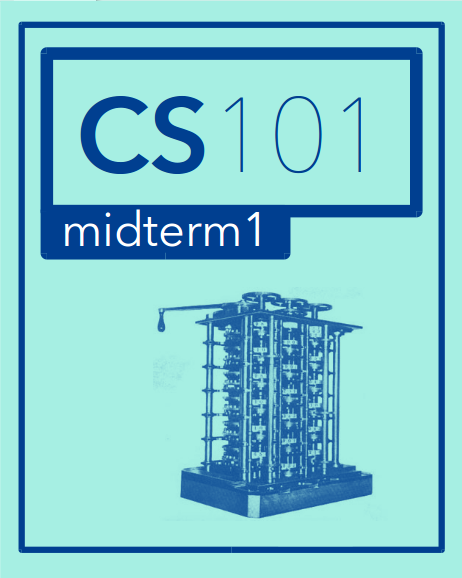
\includegraphics[width=2in]{../img/midterm1-header.png}
\end{center}

\bigskip
\noindent
\begin{itemize}
\item \textbf{Be sure to enter your \underline{NetID} and \underline{the code below} on your Scantron}.
\item Do not turn this page until instructed to do so.
\item There are 30 questions, worth 1 point each.
\item Each question has only \textbf{one} correct answer.
\item You must not communicate with other students during this test.
\item No books, notes, or electronic devices are permitted.
\item This is a 60-minute exam.
\item There are several different versions of this exam.
\end{itemize}

\bigskip\bigskip
\noindent
\textbf{\Large 1. Fill in your information:}

\bigskip
{\Large\bf
\begin{tabular}{ll}
Full Name: & \underbar{\hskip 8cm} \\[0.5em]
UIN (Student Number): & \underbar{\hskip 8cm} \\[0.5em]
NetID: & \underbar{\hskip 8cm}
\end{tabular}
}

\bigskip
\bigskip
\noindent
\textbf{\Large 2. Fill in the following answers on the Scantron form:}

%%%%%%%%%%%%%%%%%%%%%%%%%%%%%%%%%%%%%%%%%%%%%%%%%%%%%%%%%
%%%%%%%%%%%%%%%%%%%%%%%%%%%%%%%%%%%%%%%%%%%%%%%%%%%%%%%%%

\begin{enumerate}
\item[92.] E
\item[93.] D
\item[94.] A
\item[95.] A
\item[96.] C
\end{enumerate}

\newpage

% Zone 1


%%%%%%%%%%%%%%%%%%%%%%%%%%%%%%%%%%%%%%%%%%%%%%%%%%%%%%%%%



\newpage
\noindent
1. (1 point)
Consider the following program:
\begin{verbatim}
s="Calvin"
i=0
x=-1
while i<len(s):
    if s[i]=='b':
        x=i
    i+=1
\end{verbatim}
What is the \textbf{value} of \texttt{x} after this program is executed?


\begin{enumerate}
\item[(A)]
\begin{verbatim}0\end{verbatim}

\item[(B)]
\begin{verbatim}5\end{verbatim}

\item[(C)]
\begin{verbatim}3\end{verbatim}

\item[(D)]
\begin{verbatim}6\end{verbatim}

\item[(E)] $\bigstar$ 
\begin{verbatim}-1\end{verbatim}

\end{enumerate}

\vspace*{2em}
\hrule
\vspace{2em}

\noindent {\bf Solution.} 
\vspace{2em}
\hrule height 2pt


\newpage
\noindent
2. (1 point)
Consider the following program:
\begin{verbatim}
pi="3.14159"
e="2.71828"
x=pi*len(e)+pi
\end{verbatim}
What is the \textbf{type} of \texttt{x} after this program is executed?


\begin{enumerate}
\item[(A)] $\bigstar$ 
\begin{verbatim}String\end{verbatim}

\item[(B)]
\begin{verbatim}None\end{verbatim}

\item[(C)]
\begin{verbatim}Integer\end{verbatim}

\item[(D)]
\begin{verbatim}Boolean\end{verbatim}

\item[(E)]
\begin{verbatim}Float\end{verbatim}

\end{enumerate}

\vspace*{2em}
\hrule
\vspace{2em}

\noindent {\bf Solution.} 
\vspace{2em}
\hrule height 2pt


\newpage
\noindent
3. (1 point)
Consider the following program.
\begin{verbatim}
x=0
i=1
while(i*i)<=9:
    x=x+(i*i)
    i=i+1
\end{verbatim}
After it is run, what is the final \textbf{value} of \texttt{x}?


\begin{enumerate}
\item[(A)]
\begin{verbatim}5\end{verbatim}

\item[(B)]
\begin{verbatim}4\end{verbatim}

\item[(C)]
\begin{verbatim}3\end{verbatim}

\item[(D)] $\bigstar$ 
\begin{verbatim}14\end{verbatim}

\item[(E)]
\begin{verbatim}30\end{verbatim}

\end{enumerate}

\vspace*{2em}
\hrule
\vspace{2em}

\noindent {\bf Solution.} 
\vspace{2em}
\hrule height 2pt


\newpage
\noindent
4. (1 point)
Consider the following program.
\begin{verbatim}
kay = 2
wart = 3

def knight(kay,wart):
    wart += 2
    kay += 3
    return wart + kay

kay = knight(wart, kay) + knight(kay, wart)
\end{verbatim}
After it is run, what is the final \textbf{value} of \texttt{kay}?


\begin{enumerate}
\item[(A)] $\bigstar$ 
None of the other answers are correct.

\item[(B)]
\begin{verbatim}3\end{verbatim}

\item[(C)]
\begin{verbatim}2\end{verbatim}

\item[(D)]
\begin{verbatim}5\end{verbatim}

\end{enumerate}

\vspace*{2em}
\hrule
\vspace{2em}

\noindent {\bf Solution.} 
\vspace{2em}
\hrule height 2pt


\newpage
\noindent
5. (1 point)
Consider the following Python program.
\begin{verbatim}
e=[1,3,5,7,9,11]
d=[0,0,0]
for i in range(0,len(e)):
    d[i%3]+=e[i]
x=d[2]
\end{verbatim}
After it is run, what is the final \textbf{value} of \texttt{x}?


\begin{enumerate}
\item[(A)]
\begin{verbatim}7\end{verbatim}

\item[(B)]
\begin{verbatim}0\end{verbatim}

\item[(C)]
\begin{verbatim}12\end{verbatim}

\item[(D)]
\begin{verbatim}8\end{verbatim}

\item[(E)] $\bigstar$ 
\begin{verbatim}16\end{verbatim}

\end{enumerate}

\vspace*{2em}
\hrule
\vspace{2em}

\noindent {\bf Solution.} 
\vspace{2em}
\hrule height 2pt


\newpage
\noindent
6. (1 point)
Consider the following program.
\begin{verbatim}
x=[]
for j in range(0,5):
    if (j%3)==0:
        x.append("-")
    if (j%4)==0:
        x.append("*")
\end{verbatim}
After it is run, what is the final \textbf{value} of \texttt{x}?


\begin{enumerate}
\item[(A)] $\bigstar$ 
\begin{verbatim}["-","*","-","*"]\end{verbatim}

\item[(B)]
None of the other answers are correct.

\item[(C)]
\begin{verbatim}["*","-","*"]\end{verbatim}

\item[(D)]
\begin{verbatim}["*","-","*"]\end{verbatim}

\item[(E)]
\begin{verbatim}["-","*"]\end{verbatim}

\end{enumerate}

\vspace*{2em}
\hrule
\vspace{2em}

\noindent {\bf Solution.} 
\vspace{2em}
\hrule height 2pt


\newpage
\noindent
7. (1 point)
Consider the following program:
\begin{verbatim}
x=str(1.2)*2
\end{verbatim}
What is the \textbf{value} of \texttt{x} after this program is executed?


\begin{enumerate}
\item[(A)]
None of the other answers are correct.

\item[(B)]
\begin{verbatim}"2.4"\end{verbatim}

\item[(C)]
\begin{verbatim}"1.2*2"\end{verbatim}

\item[(D)] $\bigstar$ 
\begin{verbatim}"1.21.2"\end{verbatim}

\item[(E)]
\begin{verbatim}2.4\end{verbatim}

\end{enumerate}

\vspace*{2em}
\hrule
\vspace{2em}

\noindent {\bf Solution.} 
\vspace{2em}
\hrule height 2pt


\newpage
\noindent
8. (1 point)
Consider the following program:
\begin{verbatim}
s="TRIS %i"
t="ISEU"
x=len(s) % len(t[2:-1])
\end{verbatim}
What is the \textbf{type} of \texttt{x} after this program is executed?


\begin{enumerate}
\item[(A)]
\begin{verbatim}Float\end{verbatim}

\item[(B)] $\bigstar$ 
\begin{verbatim}Integer\end{verbatim}

\item[(C)]
\begin{verbatim}None\end{verbatim}

\item[(D)]
\begin{verbatim}Boolean\end{verbatim}

\item[(E)]
\begin{verbatim}String\end{verbatim}

\end{enumerate}

\vspace*{2em}
\hrule
\vspace{2em}

\noindent {\bf Solution.} 
\vspace{2em}
\hrule height 2pt


\newpage
\noindent
9. (1 point)
Consider the following program:
\begin{verbatim}
i=3
x=2
while i < 7:
    x+=i
    i+=2
\end{verbatim}
What is the \textbf{value} of \texttt{x} after this program is executed?


\begin{enumerate}
\item[(A)]
\begin{verbatim}11\end{verbatim}

\item[(B)] $\bigstar$ 
\begin{verbatim}10\end{verbatim}

\item[(C)]
\begin{verbatim}13\end{verbatim}

\item[(D)]
\begin{verbatim}14\end{verbatim}

\item[(E)]
\begin{verbatim}12\end{verbatim}

\end{enumerate}

\vspace*{2em}
\hrule
\vspace{2em}

\noindent {\bf Solution.} 
\vspace{2em}
\hrule height 2pt


\newpage
\noindent
10. (1 point)
What is the result of the following expression?
\begin{verbatim}
[ 1, 2, 3 ] * 3.0
\end{verbatim}


\begin{enumerate}
\item[(A)] $\bigstar$ 
\begin{verbatim}[1, 2, 3, 1, 2, 3, 1, 2, 3]\end{verbatim}

\item[(B)]
\begin{verbatim}[3.0, 6.0, 9.0]\end{verbatim}

\item[(C)]
\begin{verbatim}[1.0, 2.0, 3.0, 1.0, 2.0, 3.0, 1.0, 2.0, 3.0]\end{verbatim}

\item[(D)]
\begin{verbatim}None of the above.\end{verbatim}

\item[(E)]
\begin{verbatim}[3, 6, 9]\end{verbatim}

\end{enumerate}

\vspace*{2em}
\hrule
\vspace{2em}

\noindent {\bf Solution.} 
\vspace{2em}
\hrule height 2pt


\newpage
\noindent
11. (1 point)
Evaluate the following expression:
\begin{verbatim}
[1,2]*len("3")
\end{verbatim}
What value is produced?


\begin{enumerate}
\item[(A)]
\begin{verbatim}[1,2,3]\end{verbatim}

\item[(B)]
\begin{verbatim}[1,2,1]\end{verbatim}

\item[(C)]
\begin{verbatim}[1,2,1,2,1,2]\end{verbatim}

\item[(D)] $\bigstar$ 
\begin{verbatim}[1,2]\end{verbatim}

\end{enumerate}

\vspace*{2em}
\hrule
\vspace{2em}

\noindent {\bf Solution.} 
\vspace{2em}
\hrule height 2pt


\newpage
\noindent
12. (1 point)
Consider the following incomplete function.
\begin{verbatim}
def ismultiple(m,n):
    if ???:
        return False
    else:
        return True
\end{verbatim}
The function is intended to return True if the input parameter m is a multiple of parameter n and False otherwise. For example, \verb|ismultiple(4,2)| should return \verb|True|, but \verb|ismultiple(5,3)| should return \verb|False|. What should replace the three question marks to complete the function?


\begin{enumerate}
\item[(A)]
\begin{verbatim}(m // n) != 0 \end{verbatim}

\item[(B)]
\begin{verbatim}(n % m) == 0 \end{verbatim}

\item[(C)]
\begin{verbatim}(n // m) == 0 \end{verbatim}

\item[(D)] $\bigstar$ 
\begin{verbatim}(m % n) != 0 \end{verbatim}

\end{enumerate}

\vspace*{2em}
\hrule
\vspace{2em}

\noindent {\bf Solution.} 
\vspace{2em}
\hrule height 2pt


\newpage
\noindent
13. (1 point)
How can the following mathematical equation be implemented as a Python expression? Assume \verb|a|, \verb|b|, and \verb|cos| have already been defined.
$$a^b \cos(a - b)$$


\begin{enumerate}
\item[(A)] $\bigstar$ 
\begin{verbatim}(a**b)*cos(a-b)\end{verbatim}

\item[(B)]
None of the other answers are correct.

\item[(C)]
\begin{verbatim}(a**b)cos(a-b)\end{verbatim}

\item[(D)]
\begin{verbatim}(b^a)cos(a-b)\end{verbatim}

\item[(E)]
\begin{verbatim}(a^b)*cos(a-b)\end{verbatim}

\end{enumerate}

\vspace*{2em}
\hrule
\vspace{2em}

\noindent {\bf Solution.} 
\vspace{2em}
\hrule height 2pt


\newpage
\noindent
14. (1 point)
Consider the following program:
\begin{verbatim}
s="-B-O-R-S-"
x=s.split("-")[2:-2]
\end{verbatim}
What is the \textbf{value} of \texttt{x} after this program is executed?


\begin{enumerate}
\item[(A)]
\begin{verbatim}False\end{verbatim}

\item[(B)]
\begin{verbatim}'ORS'\end{verbatim}

\item[(C)] $\bigstar$ 
\begin{verbatim}['O', 'R']\end{verbatim}

\item[(D)]
\begin{verbatim}''\end{verbatim}

\item[(E)]
\begin{verbatim}None\end{verbatim}

\end{enumerate}

\vspace*{2em}
\hrule
\vspace{2em}

\noindent {\bf Solution.} 
\vspace{2em}
\hrule height 2pt


\newpage
\noindent
15. (1 point)
Consider the following incomplete Python program.
\begin{verbatim}
s="".join(["1","0","2","1"])
x=0
for i in range(len(s)-1):
    x+=int(???)
\end{verbatim}
What should replace the three question marks so the resulting value of \texttt{x} is 33?


\begin{enumerate}
\item[(A)]
\begin{verbatim}s[i:i-1]\end{verbatim}

\item[(B)]
\begin{verbatim}s[i+1:i+2]\end{verbatim}

\item[(C)]
\begin{verbatim}s[i:i+1]\end{verbatim}

\item[(D)] $\bigstar$ 
\begin{verbatim}s[i:i+2]\end{verbatim}

\end{enumerate}

\vspace*{2em}
\hrule
\vspace{2em}

\noindent {\bf Solution.} 
\vspace{2em}
\hrule height 2pt


\newpage
\noindent
16. (1 point)
Consider the following program:
\begin{verbatim}
a=["merlin","sir agravaine","king pellinore"]
b=[ ]
for i in range(1,3):
    b.append(a[0-i].title())
\end{verbatim}
What is the \textbf{value} of b after this program is executed?


\begin{enumerate}
\item[(A)]
\begin{verbatim}[ ]\end{verbatim}

\item[(B)]
\begin{verbatim}['King Pellinore', 'Sir Agravaine', 'Merlin']\end{verbatim}

\item[(C)] $\bigstar$ 
\begin{verbatim}['King Pellinore', 'Sir Agravaine']\end{verbatim}

\item[(D)]
\begin{verbatim}['Sir Agravaine', 'King Pellinore']\end{verbatim}

\item[(E)]
\begin{verbatim}['Merlin', 'King Pellinore', 'Sir Agravaine']\end{verbatim}

\end{enumerate}

\vspace*{2em}
\hrule
\vspace{2em}

\noindent {\bf Solution.} 
\vspace{2em}
\hrule height 2pt


\newpage
\noindent
17. (1 point)
Consider the following program:
\begin{verbatim}
a=["A","C","C","I","O"]
a.sort()
a[0]=a[-1]
x=""
for e in a:
    x=x+e
\end{verbatim}
What is the \textbf{value} of \texttt{x} after this program is executed?


\begin{enumerate}
\item[(A)] $\bigstar$ 
\begin{verbatim}"OCCIO"\end{verbatim}

\item[(B)]
\begin{verbatim}"ICCOI"\end{verbatim}

\item[(C)]
\begin{verbatim}"ACCOA"\end{verbatim}

\item[(D)]
None of the other answers are correct.

\item[(E)]
\begin{verbatim}"ACCIA"\end{verbatim}

\end{enumerate}

\vspace*{2em}
\hrule
\vspace{2em}

\noindent {\bf Solution.} 
\vspace{2em}
\hrule height 2pt


\newpage
\noindent
18. (1 point)
Consider the following program:
\begin{verbatim}
a=3
b=4
if a==3:
    b=a
elif a==4:
    a=5
else:
    a=b
\end{verbatim}
What is the \textbf{value} of a after this program is executed?


\begin{enumerate}
\item[(A)]
\begin{verbatim}5\end{verbatim}

\item[(B)]
\begin{verbatim}4\end{verbatim}

\item[(C)]
None of the other answers are correct.

\item[(D)]
\begin{verbatim}7\end{verbatim}

\item[(E)] $\bigstar$ 
\begin{verbatim}3\end{verbatim}

\end{enumerate}

\vspace*{2em}
\hrule
\vspace{2em}

\noindent {\bf Solution.} 
\vspace{2em}
\hrule height 2pt


\newpage
\noindent
19. (1 point)
Consider the following program:
\begin{verbatim}
s="ECTOR"
t="GAWAIN"
x=(len(s)+len(t)) < 4 and s in t
\end{verbatim}
What is the \textbf{type} of \texttt{x} after this program is executed?


\begin{enumerate}
\item[(A)]
\begin{verbatim}Integer\end{verbatim}

\item[(B)]
\begin{verbatim}None\end{verbatim}

\item[(C)]
\begin{verbatim}String\end{verbatim}

\item[(D)]
\begin{verbatim}Float\end{verbatim}

\item[(E)] $\bigstar$ 
\begin{verbatim}Boolean\end{verbatim}

\end{enumerate}

\vspace*{2em}
\hrule
\vspace{2em}

\noindent {\bf Solution.} 
\vspace{2em}
\hrule height 2pt


\newpage
\noindent
20. (1 point)
Consider the following program.
\begin{verbatim}
def artificing(s):
    return s*2
    return s+"%i" % 2
    return s

s=artificing("MERLIN")
\end{verbatim}
After it is run, what is the final \textbf{value} of s?


\begin{enumerate}
\item[(A)]
\begin{verbatim}"MERLIN"\end{verbatim}

\item[(B)]
\begin{verbatim}None\end{verbatim}

\item[(C)]
\begin{verbatim}12\end{verbatim}

\item[(D)]
\begin{verbatim}"MERLIN2"\end{verbatim}

\item[(E)] $\bigstar$ 
\begin{verbatim}"MERLINMERLIN"\end{verbatim}

\end{enumerate}

\vspace*{2em}
\hrule
\vspace{2em}

\noindent {\bf Solution.} 
\vspace{2em}
\hrule height 2pt


\newpage
\noindent
21. (1 point)
Consider the following program.
\begin{verbatim}
s="BBCAA"
x=0
y=len(s)-1
while s[x]!=s[y] and x<len(s):
    x+=1
    y-=1
\end{verbatim}
After it is run, what is the final \textbf{value} of \texttt{x}?


\begin{enumerate}
\item[(A)] $\bigstar$ 
\begin{verbatim}2\end{verbatim}

\item[(B)]
\begin{verbatim}0\end{verbatim}

\item[(C)]
\begin{verbatim}4\end{verbatim}

\item[(D)]
\begin{verbatim}3\end{verbatim}

\item[(E)]
\begin{verbatim}1\end{verbatim}

\end{enumerate}

\vspace*{2em}
\hrule
\vspace{2em}

\noindent {\bf Solution.} 
\vspace{2em}
\hrule height 2pt


\newpage
\noindent
22. (1 point)
Consider the following program:
\begin{verbatim}
x=[1,2,3]
def f(a):
    s=""
    a.append(4)
    for i in a:
        s+=str(i)
    return s

x.append(f(x))
\end{verbatim}
What is the \textbf{value} of \texttt{x} after this program is executed?


\begin{enumerate}
\item[(A)] $\bigstar$ 
\begin{verbatim}[1, 2, 3, 4, '1234']\end{verbatim}

\item[(B)]
\begin{verbatim}[1, 2, 3, '123']\end{verbatim}

\item[(C)]
\begin{verbatim}[1, 2, 3, '1234']\end{verbatim}

\item[(D)]
\begin{verbatim}[1, 2, 3]\end{verbatim}

\item[(E)]
\begin{verbatim}[1, 2, 3, 10]\end{verbatim}

\end{enumerate}

\vspace*{2em}
\hrule
\vspace{2em}

\noindent {\bf Solution.} 
\vspace{2em}
\hrule height 2pt


\newpage
\noindent
23. (1 point)
Consider the following program:
\begin{verbatim}
x="KING ARTHUR-MORGANA LEFAY-SIR BEDIVERE".split("-")
y=x[:]
y.reverse()
\end{verbatim}
What is the \textbf{value} of \texttt{x} after this program is executed?


\begin{enumerate}
\item[(A)] $\bigstar$ 
\begin{verbatim}['KING ARTHUR', 'MORGANA LEFAY', 'SIR BEDIVERE']\end{verbatim}

\item[(B)]
\begin{verbatim}['BEDIVERE', 'LEFAY-SIR', 'ARTHUR-MORGANA', 'KING']\end{verbatim}

\item[(C)]
\begin{verbatim}None\end{verbatim}

\item[(D)]
\begin{verbatim}['SIR BEDIVERE', 'MORGANA LEFAY', 'KING ARTHUR']\end{verbatim}

\item[(E)]
\begin{verbatim}['KING', 'ARTHUR-MORGANA', 'LEFAY-SIR', 'BEDIVERE']\end{verbatim}

\end{enumerate}

\vspace*{2em}
\hrule
\vspace{2em}

\noindent {\bf Solution.} 
\vspace{2em}
\hrule height 2pt


\newpage
\noindent
24. (1 point)
Consider the following incomplete program.
\begin{verbatim}
sum=0
for i in range(0,100):
    ???

\end{verbatim}
The program is intended to sum all of the integers between 1 and 100 (inclusive). What should replace the three question marks to complete the program?


\begin{enumerate}
\item[(A)]
\begin{verbatim}sum+1=sum \end{verbatim}

\item[(B)] $\bigstar$ 
\begin{verbatim}sum=sum+i+1 \end{verbatim}

\item[(C)]
\begin{verbatim}sum=sum+i \end{verbatim}

\item[(D)]
\begin{verbatim}sum=sum+1\end{verbatim}

\end{enumerate}

\vspace*{2em}
\hrule
\vspace{2em}

\noindent {\bf Solution.} 
\vspace{2em}
\hrule height 2pt


\newpage
\noindent
25. (1 point)
For this problem, you should compose a function which accomplishes a given task using the available code blocks arranged in the correct functional order.  \emph{We ignore indentation for this problem.}

\texttt{find\_max} should accept a \texttt{list} and return the value of the maximum item in the \texttt{list}.  (\texttt{None} is always the lowest value in any numeric comparison, so you may use it as an initializer.)

\begin{verbatim}
def find_max(my_list):
\end{verbatim}

\begin{enumerate}[1]
\item \texttt{max\_val = i}
\item \texttt{max\_val = None}
\item \texttt{for i in range(len(my\_list)):}
\item \texttt{if i > max\_val:}
\item \texttt{max\_val = my\_list[i]}
\item \texttt{return max\_val}
\item \texttt{for i in range(my\_list):}
\item \texttt{if my\_list[i] > max\_val:}
\item \texttt{print(max\_val)}
\end{enumerate}



\begin{enumerate}
\item[(A)]
3, 2, 8, 5, 9

\item[(B)] $\bigstar$ 
2, 3, 8, 5, 6

\item[(C)]
2, 3, 8, 1, 6

\item[(D)]
2, 7, 4, 5, 6

\item[(E)]
2, 3, 4, 1, 6

\end{enumerate}

\vspace*{2em}
\hrule
\vspace{2em}

\noindent {\bf Solution.} 
\vspace{2em}
\hrule height 2pt


\newpage
\noindent
26. (1 point)
Evaluate the following expression:
\begin{verbatim}
len("ABCDE"[1:4])
\end{verbatim}
What value is produced?


\begin{enumerate}
\item[(A)]
1

\item[(B)] $\bigstar$ 
3

\item[(C)]
5

\item[(D)]
4

\end{enumerate}

\vspace*{2em}
\hrule
\vspace{2em}

\noindent {\bf Solution.} 
\vspace{2em}
\hrule height 2pt


\newpage
\noindent
27. (1 point)
Consider the following program:
\begin{verbatim}
x=0
for i in range(4,10):
    if i%3==0:
        x+=3
    elif i%2==0:
        x+=2
    else:
        x+=1
\end{verbatim}
What is the \textbf{value} of \texttt{x} after this program is executed?


\begin{enumerate}
\item[(A)]
\begin{verbatim}10\end{verbatim}

\item[(B)]
\begin{verbatim}13\end{verbatim}

\item[(C)]
\begin{verbatim}14\end{verbatim}

\item[(D)] $\bigstar$ 
\begin{verbatim}12\end{verbatim}

\item[(E)]
\begin{verbatim}11\end{verbatim}

\end{enumerate}

\vspace*{2em}
\hrule
\vspace{2em}

\noindent {\bf Solution.} 
\vspace{2em}
\hrule height 2pt


\newpage
\noindent
28. (1 point)
Consider the following program:
\begin{verbatim}
x=3
a=7
if (a%3)==2:
    x=x**2
elif(a%3)==1:
    x=x**1
else:
    x=x**0
\end{verbatim}
What is the \textbf{value} of \texttt{x} after this program is executed?


\begin{enumerate}
\item[(A)]
\begin{verbatim}1\end{verbatim}

\item[(B)] $\bigstar$ 
\begin{verbatim}3\end{verbatim}

\item[(C)]
\begin{verbatim}7\end{verbatim}

\item[(D)]
None of the other answers are correct.

\item[(E)]
\begin{verbatim}9\end{verbatim}

\end{enumerate}

\vspace*{2em}
\hrule
\vspace{2em}

\noindent {\bf Solution.} 
\vspace{2em}
\hrule height 2pt


\newpage
\noindent
29. (1 point)
Consider the following program:
\begin{verbatim}
x=[1,2,3,4,5,6,7,8,9]
x=x[2:-2]
i=1
while i <= 3:
    x[i]+=1
    i+=1
\end{verbatim}
What is the \textbf{value} of \texttt{x} after this program is executed?


\begin{enumerate}
\item[(A)]
\begin{verbatim}[2, 4, 5, 6, 7, 7]\end{verbatim}

\item[(B)]
\begin{verbatim}[3, 5, 7, 7]\end{verbatim}

\item[(C)]
\begin{verbatim}[3, 5, 6, 7, 7, 8]\end{verbatim}

\item[(D)] $\bigstar$ 
\begin{verbatim}[3, 5, 6, 7, 7]\end{verbatim}

\item[(E)]
\begin{verbatim}[2, 4, 5, 5, 7, 7]\end{verbatim}

\end{enumerate}

\vspace*{2em}
\hrule
\vspace{2em}

\noindent {\bf Solution.} 
\vspace{2em}
\hrule height 2pt


\newpage
\noindent
30. (1 point)
Consider the following program:
\begin{verbatim}
def fix(s):
    a=list(s)
    a.sort()
    return ''.join(a)

x=["one","two","eleven","twelve"]
s1=fix(x[0]+x[-1])
s2=fix(x[1]+x[-2])

if s1==s2:
    x.sort()
elif s1<s2:
    x.reverse()
else:
    x.append("six")
\end{verbatim}
What is the \textbf{value} of \texttt{x} after this program is executed?


\begin{enumerate}
\item[(A)] $\bigstar$ 
\begin{verbatim}['eleven', 'one', 'twelve', 'two']\end{verbatim}

\item[(B)]
\begin{verbatim}['twelve', 'eleven', 'two', 'one']\end{verbatim}

\item[(C)]
\begin{verbatim}['one', 'two', 'eleven', 'twelve']\end{verbatim}

\item[(D)]
\begin{verbatim}['one', 'two', 'eleven', 'twelve', 'six']\end{verbatim}

\item[(E)]
\begin{verbatim}['two', 'twelve', 'one', 'eleven', 'six']\end{verbatim}

\end{enumerate}

\vspace*{2em}
\hrule
\vspace{2em}

\noindent {\bf Solution.} 
\vspace{2em}
\hrule height 2pt

%%%%%%%%%%%%%%%%%%%%%%%%%%%%%%%%%%%%%%%%%%%%%%%%%%%%%%%%%%%%%%%%%%%%%%
%%%%%%%%%%%%%%%%%%%%%%%%%%%%%%%%%%%%%%%%%%%%%%%%%%%%%%%%%%%%%%%%%%%%%%
%%%%%%%%%%%%%%%%%%%%%%%%%%%%%%%%%%%%%%%%%%%%%%%%%%%%%%%%%%%%%%%%%%%%%%
%%%%%%%%%%%%%%%%%%%%%%%%%%%%%%%%%%%%%%%%%%%%%%%%%%%%%%%%%%%%%%%%%%%%%%
% Exam number 21

\message{Exam 21/50}
\cleardoublepage
\setcounter{page}{1}


\begin{center}
%\textbf{\Large CS 101 Midterm \#1}
%
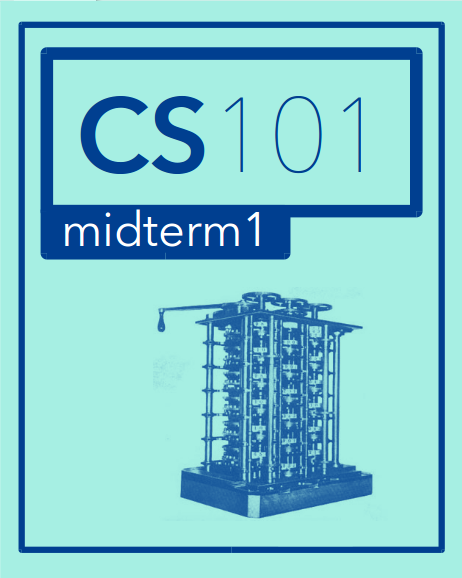
\includegraphics[width=2in]{../img/midterm1-header.png}
\end{center}

\bigskip
\noindent
\begin{itemize}
\item \textbf{Be sure to enter your \underline{NetID} and \underline{the code below} on your Scantron}.
\item Do not turn this page until instructed to do so.
\item There are 30 questions, worth 1 point each.
\item Each question has only \textbf{one} correct answer.
\item You must not communicate with other students during this test.
\item No books, notes, or electronic devices are permitted.
\item This is a 60-minute exam.
\item There are several different versions of this exam.
\end{itemize}

\bigskip\bigskip
\noindent
\textbf{\Large 1. Fill in your information:}

\bigskip
{\Large\bf
\begin{tabular}{ll}
Full Name: & \underbar{\hskip 8cm} \\[0.5em]
UIN (Student Number): & \underbar{\hskip 8cm} \\[0.5em]
NetID: & \underbar{\hskip 8cm}
\end{tabular}
}

\bigskip
\bigskip
\noindent
\textbf{\Large 2. Fill in the following answers on the Scantron form:}

%%%%%%%%%%%%%%%%%%%%%%%%%%%%%%%%%%%%%%%%%%%%%%%%%%%%%%%%%
%%%%%%%%%%%%%%%%%%%%%%%%%%%%%%%%%%%%%%%%%%%%%%%%%%%%%%%%%

\begin{enumerate}
\item[92.] A
\item[93.] E
\item[94.] A
\item[95.] C
\item[96.] A
\end{enumerate}

\newpage

% Zone 1


%%%%%%%%%%%%%%%%%%%%%%%%%%%%%%%%%%%%%%%%%%%%%%%%%%%%%%%%%



\newpage
\noindent
1. (1 point)
For this problem, you should compose a function which accomplishes a given task using the available code blocks arranged in the correct functional order.  \emph{We ignore indentation for this problem.}

\texttt{find\_max} should accept a \texttt{list} and return the value of the maximum item in the \texttt{list}.  (\texttt{None} is always the lowest value in any numeric comparison, so you may use it as an initializer.)

\begin{verbatim}
def find_max(my_list):
\end{verbatim}

\begin{enumerate}[1]
\item \texttt{max\_val = i}
\item \texttt{max\_val = None}
\item \texttt{for i in range(len(my\_list)):}
\item \texttt{if i > max\_val:}
\item \texttt{max\_val = my\_list[i]}
\item \texttt{return max\_val}
\item \texttt{for i in range(my\_list):}
\item \texttt{if my\_list[i] > max\_val:}
\item \texttt{print(max\_val)}
\end{enumerate}



\begin{enumerate}
\item[(A)]
2, 7, 4, 5, 6

\item[(B)]
3, 2, 8, 5, 9

\item[(C)]
2, 3, 4, 1, 6

\item[(D)] $\bigstar$ 
2, 3, 8, 5, 6

\item[(E)]
2, 3, 8, 1, 6

\end{enumerate}

\vspace*{2em}
\hrule
\vspace{2em}

\noindent {\bf Solution.} 
\vspace{2em}
\hrule height 2pt


\newpage
\noindent
2. (1 point)
Consider the following program.
\begin{verbatim}
def artificing(s):
    return s+"%i" % 2
    return s*2
    return s

s=artificing("MERLIN")
\end{verbatim}
After it is run, what is the final \textbf{value} of s?


\begin{enumerate}
\item[(A)] $\bigstar$ 
\begin{verbatim}"MERLIN2"\end{verbatim}

\item[(B)]
\begin{verbatim}None\end{verbatim}

\item[(C)]
\begin{verbatim}0\end{verbatim}

\item[(D)]
\begin{verbatim}"MERLINMERLIN"\end{verbatim}

\item[(E)]
\begin{verbatim}"MERLIN%i"\end{verbatim}

\end{enumerate}

\vspace*{2em}
\hrule
\vspace{2em}

\noindent {\bf Solution.} 
\vspace{2em}
\hrule height 2pt


\newpage
\noindent
3. (1 point)
Consider the following program.
\begin{verbatim}
s="BBCAA"
x=0
y=len(s)-1
while s[x]!=s[y] and x<len(s):
    x+=1
    y-=1
\end{verbatim}
After it is run, what is the final \textbf{value} of \texttt{x}?


\begin{enumerate}
\item[(A)]
\begin{verbatim}4\end{verbatim}

\item[(B)]
\begin{verbatim}1\end{verbatim}

\item[(C)] $\bigstar$ 
\begin{verbatim}2\end{verbatim}

\item[(D)]
\begin{verbatim}0\end{verbatim}

\item[(E)]
\begin{verbatim}3\end{verbatim}

\end{enumerate}

\vspace*{2em}
\hrule
\vspace{2em}

\noindent {\bf Solution.} 
\vspace{2em}
\hrule height 2pt


\newpage
\noindent
4. (1 point)
Consider the following program:
\begin{verbatim}
a=["A","C","C","I","O"]
a.sort()
a[0]=a[-1]
x=""
for e in a:
    x=x+e
\end{verbatim}
What is the \textbf{value} of \texttt{x} after this program is executed?


\begin{enumerate}
\item[(A)]
\begin{verbatim}"ACCOA"\end{verbatim}

\item[(B)] $\bigstar$ 
\begin{verbatim}"OCCIO"\end{verbatim}

\item[(C)]
\begin{verbatim}"ICCOI"\end{verbatim}

\item[(D)]
\begin{verbatim}"ACCIA"\end{verbatim}

\item[(E)]
None of the other answers are correct.

\end{enumerate}

\vspace*{2em}
\hrule
\vspace{2em}

\noindent {\bf Solution.} 
\vspace{2em}
\hrule height 2pt


\newpage
\noindent
5. (1 point)
Consider the following program:
\begin{verbatim}
a=["merlin","sir agravaine","king pellinore"]
b=[ ]
for i in range(0,3):
    b.append(a[0-i].title())
\end{verbatim}
What is the \textbf{value} of b after this program is executed?


\begin{enumerate}
\item[(A)]
\begin{verbatim}['Sir Agravaine', 'King Pellinore']\end{verbatim}

\item[(B)]
\begin{verbatim}[ ]\end{verbatim}

\item[(C)] $\bigstar$ 
\begin{verbatim}['Merlin', 'King Pellinore', 'Sir Agravaine']\end{verbatim}

\item[(D)]
\begin{verbatim}['King Pellinore', 'Sir Agravaine', 'Merlin']\end{verbatim}

\item[(E)]
\begin{verbatim}['King Pellinore', 'Sir Agravaine']\end{verbatim}

\end{enumerate}

\vspace*{2em}
\hrule
\vspace{2em}

\noindent {\bf Solution.} 
\vspace{2em}
\hrule height 2pt


\newpage
\noindent
6. (1 point)
Evaluate the following expression:
\begin{verbatim}
[1,2]+[len("3")]
\end{verbatim}
What value is produced?


\begin{enumerate}
\item[(A)]
\begin{verbatim}[1,2,3]\end{verbatim}

\item[(B)]
\begin{verbatim}[1,2,"3"]\end{verbatim}

\item[(C)]
\begin{verbatim}[1,2,1,2,1,2]\end{verbatim}

\item[(D)] $\bigstar$ 
\begin{verbatim}[1,2,1]\end{verbatim}

\end{enumerate}

\vspace*{2em}
\hrule
\vspace{2em}

\noindent {\bf Solution.} 
\vspace{2em}
\hrule height 2pt


\newpage
\noindent
7. (1 point)
Consider the following program:
\begin{verbatim}
x=0
for i in range(2,8):
    if i%3==0:
        x+=3
    elif i%2==0:
        x+=2
    else:
        x+=1
\end{verbatim}
What is the \textbf{value} of \texttt{x} after this program is executed?


\begin{enumerate}
\item[(A)]
\begin{verbatim}11\end{verbatim}

\item[(B)]
\begin{verbatim}13\end{verbatim}

\item[(C)]
\begin{verbatim}14\end{verbatim}

\item[(D)]
\begin{verbatim}10\end{verbatim}

\item[(E)] $\bigstar$ 
\begin{verbatim}12\end{verbatim}

\end{enumerate}

\vspace*{2em}
\hrule
\vspace{2em}

\noindent {\bf Solution.} 
\vspace{2em}
\hrule height 2pt


\newpage
\noindent
8. (1 point)
Consider the following incomplete Python program.
\begin{verbatim}
s="".join(["1","0","2","1"])
x=0
for i in range(len(s)-1):
    x+=int(???)
\end{verbatim}
What should replace the three question marks so the resulting value of \texttt{x} is 33?


\begin{enumerate}
\item[(A)] $\bigstar$ 
\begin{verbatim}s[i:i+2]\end{verbatim}

\item[(B)]
\begin{verbatim}s[i:i+1]\end{verbatim}

\item[(C)]
\begin{verbatim}s[i:i-1]\end{verbatim}

\item[(D)]
\begin{verbatim}s[i+1:i+2]\end{verbatim}

\end{enumerate}

\vspace*{2em}
\hrule
\vspace{2em}

\noindent {\bf Solution.} 
\vspace{2em}
\hrule height 2pt


\newpage
\noindent
9. (1 point)
What is the result of the following expression?
\begin{verbatim}
[ 1, 2, 3 ] * 3.0
\end{verbatim}


\begin{enumerate}
\item[(A)]
\begin{verbatim}[3.0, 6.0, 9.0]\end{verbatim}

\item[(B)]
\begin{verbatim}[3, 6, 9]\end{verbatim}

\item[(C)]
\begin{verbatim}None of the above.\end{verbatim}

\item[(D)]
\begin{verbatim}[1.0, 2.0, 3.0, 1.0, 2.0, 3.0, 1.0, 2.0, 3.0]\end{verbatim}

\item[(E)] $\bigstar$ 
\begin{verbatim}[1, 2, 3, 1, 2, 3, 1, 2, 3]\end{verbatim}

\end{enumerate}

\vspace*{2em}
\hrule
\vspace{2em}

\noindent {\bf Solution.} 
\vspace{2em}
\hrule height 2pt


\newpage
\noindent
10. (1 point)
Consider the following program:
\begin{verbatim}
s="ECTOR"
t="GAWAIN"
x=(len(s)/(len(t)-1))+1
\end{verbatim}
What is the \textbf{type} of \texttt{x} after this program is executed?


\begin{enumerate}
\item[(A)]
\begin{verbatim}Integer\end{verbatim}

\item[(B)]
\begin{verbatim}Boolean\end{verbatim}

\item[(C)] $\bigstar$ 
\begin{verbatim}Float\end{verbatim}

\item[(D)]
\begin{verbatim}None\end{verbatim}

\item[(E)]
\begin{verbatim}String\end{verbatim}

\end{enumerate}

\vspace*{2em}
\hrule
\vspace{2em}

\noindent {\bf Solution.} 
\vspace{2em}
\hrule height 2pt


\newpage
\noindent
11. (1 point)
Consider the following incomplete function.
\begin{verbatim}
def ismultiple(m,n):
    if ???:
        return False
    else:
        return True
\end{verbatim}
The function is intended to return True if the input parameter m is a multiple of parameter n and False otherwise. For example, \verb|ismultiple(4,2)| should return \verb|True|, but \verb|ismultiple(5,3)| should return \verb|False|. What should replace the three question marks to complete the function?


\begin{enumerate}
\item[(A)] $\bigstar$ 
\begin{verbatim}(m % n) != 0 \end{verbatim}

\item[(B)]
\begin{verbatim}(m // n) != 0 \end{verbatim}

\item[(C)]
\begin{verbatim}(n % m) == 0 \end{verbatim}

\item[(D)]
\begin{verbatim}(n // m) == 0 \end{verbatim}

\end{enumerate}

\vspace*{2em}
\hrule
\vspace{2em}

\noindent {\bf Solution.} 
\vspace{2em}
\hrule height 2pt


\newpage
\noindent
12. (1 point)
Consider the following program:
\begin{verbatim}
pi="3.14159"
e="2.71828"
x=(float(e)**float(pi)-float(pi)) == 20
\end{verbatim}
What is the \textbf{type} of \texttt{x} after this program is executed?


\begin{enumerate}
\item[(A)] $\bigstar$ 
\begin{verbatim}Boolean\end{verbatim}

\item[(B)]
\begin{verbatim}Float\end{verbatim}

\item[(C)]
\begin{verbatim}String\end{verbatim}

\item[(D)]
\begin{verbatim}Integer\end{verbatim}

\item[(E)]
\begin{verbatim}None\end{verbatim}

\end{enumerate}

\vspace*{2em}
\hrule
\vspace{2em}

\noindent {\bf Solution.} 
\vspace{2em}
\hrule height 2pt


\newpage
\noindent
13. (1 point)
Consider the following program:
\begin{verbatim}
s="Hobbes"
i=0
x=-1
while i<len(s):
    if s[i]=='b':
        x=i
    i+=1
\end{verbatim}
What is the \textbf{value} of \texttt{x} after this program is executed?


\begin{enumerate}
\item[(A)] $\bigstar$ 
\begin{verbatim}3\end{verbatim}

\item[(B)]
\begin{verbatim}4\end{verbatim}

\item[(C)]
\begin{verbatim}2\end{verbatim}

\item[(D)]
\begin{verbatim}-1\end{verbatim}

\item[(E)]
\begin{verbatim}5\end{verbatim}

\end{enumerate}

\vspace*{2em}
\hrule
\vspace{2em}

\noindent {\bf Solution.} 
\vspace{2em}
\hrule height 2pt


\newpage
\noindent
14. (1 point)
Consider the following program:
\begin{verbatim}
s="TRIS %i"
t="ISEU"
x=len(s) % len(t[2:-1])
\end{verbatim}
What is the \textbf{type} of \texttt{x} after this program is executed?


\begin{enumerate}
\item[(A)]
\begin{verbatim}Float\end{verbatim}

\item[(B)]
\begin{verbatim}None\end{verbatim}

\item[(C)]
\begin{verbatim}String\end{verbatim}

\item[(D)] $\bigstar$ 
\begin{verbatim}Integer\end{verbatim}

\item[(E)]
\begin{verbatim}Boolean\end{verbatim}

\end{enumerate}

\vspace*{2em}
\hrule
\vspace{2em}

\noindent {\bf Solution.} 
\vspace{2em}
\hrule height 2pt


\newpage
\noindent
15. (1 point)
Consider the following program.
\begin{verbatim}
x=0
i=1
while(i*i)<=9:
    x=x+(i*i)
    i=i+1
\end{verbatim}
After it is run, what is the final \textbf{value} of \texttt{x}?


\begin{enumerate}
\item[(A)]
\begin{verbatim}4\end{verbatim}

\item[(B)]
\begin{verbatim}5\end{verbatim}

\item[(C)] $\bigstar$ 
\begin{verbatim}14\end{verbatim}

\item[(D)]
\begin{verbatim}30\end{verbatim}

\item[(E)]
\begin{verbatim}3\end{verbatim}

\end{enumerate}

\vspace*{2em}
\hrule
\vspace{2em}

\noindent {\bf Solution.} 
\vspace{2em}
\hrule height 2pt


\newpage
\noindent
16. (1 point)
Consider the following program.
\begin{verbatim}
kay = 2
wart = 3

def knight(kay,wart):
    wart += 2
    kay += 3
    return wart + kay

wart = knight(kay, kay) + knight(wart, wart)
\end{verbatim}
After it is run, what is the final \textbf{value} of \texttt{wart}?


\begin{enumerate}
\item[(A)]
\begin{verbatim}5\end{verbatim}

\item[(B)]
\begin{verbatim}3\end{verbatim}

\item[(C)]
\begin{verbatim}2\end{verbatim}

\item[(D)] $\bigstar$ 
None of the other answers are correct.

\end{enumerate}

\vspace*{2em}
\hrule
\vspace{2em}

\noindent {\bf Solution.} 
\vspace{2em}
\hrule height 2pt


\newpage
\noindent
17. (1 point)
Consider the following Python program.
\begin{verbatim}
e=[1,3,5,7,9,11]
d=[0,0,0]
for i in range(0,len(e)):
    d[i%3]+=e[i]
x=d[2]
\end{verbatim}
After it is run, what is the final \textbf{value} of \texttt{x}?


\begin{enumerate}
\item[(A)]
\begin{verbatim}8\end{verbatim}

\item[(B)] $\bigstar$ 
\begin{verbatim}16\end{verbatim}

\item[(C)]
\begin{verbatim}12\end{verbatim}

\item[(D)]
\begin{verbatim}0\end{verbatim}

\item[(E)]
\begin{verbatim}7\end{verbatim}

\end{enumerate}

\vspace*{2em}
\hrule
\vspace{2em}

\noindent {\bf Solution.} 
\vspace{2em}
\hrule height 2pt


\newpage
\noindent
18. (1 point)
Consider the following program:
\begin{verbatim}
i=2
x=3
while i < 7:
    x+=i
    i+=2
\end{verbatim}
What is the \textbf{value} of \texttt{x} after this program is executed?


\begin{enumerate}
\item[(A)]
\begin{verbatim}12\end{verbatim}

\item[(B)]
\begin{verbatim}11\end{verbatim}

\item[(C)] $\bigstar$ 
\begin{verbatim}15\end{verbatim}

\item[(D)]
\begin{verbatim}13\end{verbatim}

\item[(E)]
\begin{verbatim}14\end{verbatim}

\end{enumerate}

\vspace*{2em}
\hrule
\vspace{2em}

\noindent {\bf Solution.} 
\vspace{2em}
\hrule height 2pt


\newpage
\noindent
19. (1 point)
Consider the following incomplete program.
\begin{verbatim}
sum=0
???:
    sum=sum+i

\end{verbatim}
The program is intended to sum all of the integers between 1 and 100 (inclusive). What should replace the three question marks to complete the program?


\begin{enumerate}
\item[(A)] $\bigstar$ 
\begin{verbatim}for i in range(1,101) \end{verbatim}

\item[(B)]
\begin{verbatim}for i in range(0,100)\end{verbatim}

\item[(C)]
\begin{verbatim}while i<=100 \end{verbatim}

\item[(D)]
\begin{verbatim}while i in range(100)\end{verbatim}

\end{enumerate}

\vspace*{2em}
\hrule
\vspace{2em}

\noindent {\bf Solution.} 
\vspace{2em}
\hrule height 2pt


\newpage
\noindent
20. (1 point)
Consider the following program:
\begin{verbatim}
x="KING ARTHUR-MORGANA LEFAY-SIR BEDIVERE".split("-")
y=x
y.reverse()
\end{verbatim}
What is the \textbf{value} of \texttt{x} after this program is executed?


\begin{enumerate}
\item[(A)]
\begin{verbatim}None\end{verbatim}

\item[(B)]
\begin{verbatim}['KING', 'ARTHUR-MORGANA', 'LEFAY-SIR', 'BEDIVERE']\end{verbatim}

\item[(C)] $\bigstar$ 
\begin{verbatim}['SIR BEDIVERE', 'MORGANA LEFAY', 'KING ARTHUR']\end{verbatim}

\item[(D)]
\begin{verbatim}['BEDIVERE', 'LEFAY-SIR', 'ARTHUR-MORGANA', 'KING']\end{verbatim}

\item[(E)]
\begin{verbatim}['KING ARTHUR', 'MORGANA LEFAY', 'SIR BEDIVERE']\end{verbatim}

\end{enumerate}

\vspace*{2em}
\hrule
\vspace{2em}

\noindent {\bf Solution.} 
\vspace{2em}
\hrule height 2pt


\newpage
\noindent
21. (1 point)
Consider the following program:
\begin{verbatim}
s="-B-O-R-S-"
x=s.split("-")[2:-2]
\end{verbatim}
What is the \textbf{value} of \texttt{x} after this program is executed?


\begin{enumerate}
\item[(A)]
\begin{verbatim}''\end{verbatim}

\item[(B)]
\begin{verbatim}'ORS'\end{verbatim}

\item[(C)]
\begin{verbatim}None\end{verbatim}

\item[(D)]
\begin{verbatim}False\end{verbatim}

\item[(E)] $\bigstar$ 
\begin{verbatim}['O', 'R']\end{verbatim}

\end{enumerate}

\vspace*{2em}
\hrule
\vspace{2em}

\noindent {\bf Solution.} 
\vspace{2em}
\hrule height 2pt


\newpage
\noindent
22. (1 point)
Consider the following program:
\begin{verbatim}
x=[1,2,3]
def f(a):
    s=""
    a.reverse()
    for i in a:
        s+=str(i)
    return s

x.append(f(x))
\end{verbatim}
What is the \textbf{value} of \texttt{x} after this program is executed?


\begin{enumerate}
\item[(A)]
\begin{verbatim}[1, 2, 3, 6]\end{verbatim}

\item[(B)]
\begin{verbatim}[3, 2, 1]\end{verbatim}

\item[(C)]
\begin{verbatim}[1, 2, 3, '321']\end{verbatim}

\item[(D)]
\begin{verbatim}[1, 2, 3]\end{verbatim}

\item[(E)] $\bigstar$ 
\begin{verbatim}[3, 2, 1, '321']\end{verbatim}

\end{enumerate}

\vspace*{2em}
\hrule
\vspace{2em}

\noindent {\bf Solution.} 
\vspace{2em}
\hrule height 2pt


\newpage
\noindent
23. (1 point)
\begin{verbatim}
x=str(3)+"str(3)"
\end{verbatim}
What is the \textbf{value} of \texttt{x} after this program is executed?


\begin{enumerate}
\item[(A)]
\begin{verbatim}"333"\end{verbatim}

\item[(B)]
None of the other answers are correct.

\item[(C)] $\bigstar$ 
\begin{verbatim}"3str(3)"\end{verbatim}

\item[(D)]
\begin{verbatim}"33"\end{verbatim}

\item[(E)]
\begin{verbatim}33\end{verbatim}

\end{enumerate}

\vspace*{2em}
\hrule
\vspace{2em}

\noindent {\bf Solution.} 
\vspace{2em}
\hrule height 2pt


\newpage
\noindent
24. (1 point)
Consider the following program:
\begin{verbatim}
a=3
b=4
if a==3:
    b=a
elif a==4:
    a=5
else:
    a=b
\end{verbatim}
What is the \textbf{value} of a after this program is executed?


\begin{enumerate}
\item[(A)]
\begin{verbatim}4\end{verbatim}

\item[(B)] $\bigstar$ 
\begin{verbatim}3\end{verbatim}

\item[(C)]
\begin{verbatim}5\end{verbatim}

\item[(D)]
None of the other answers are correct.

\item[(E)]
\begin{verbatim}7\end{verbatim}

\end{enumerate}

\vspace*{2em}
\hrule
\vspace{2em}

\noindent {\bf Solution.} 
\vspace{2em}
\hrule height 2pt


\newpage
\noindent
25. (1 point)
Consider the following program.
\begin{verbatim}
x=[]
for j in range(0,5):
    if (j%2)==0:
        x.append("-")
    if (j%5)==0:
        x.append("*")
\end{verbatim}
After it is run, what is the final \textbf{value} of \texttt{x}?


\begin{enumerate}
\item[(A)]
\begin{verbatim}["*","-","*","*"]\end{verbatim}

\item[(B)]
None of the other answers are correct.

\item[(C)]
\begin{verbatim}["-","-","*"]\end{verbatim}

\item[(D)]
\begin{verbatim}["-","*","-"]\end{verbatim}

\item[(E)] $\bigstar$ 
\begin{verbatim}["-","*","-","-"]\end{verbatim}

\end{enumerate}

\vspace*{2em}
\hrule
\vspace{2em}

\noindent {\bf Solution.} 
\vspace{2em}
\hrule height 2pt


\newpage
\noindent
26. (1 point)
How can the following mathematical equation be implemented as a Python expression? Assume \verb|a|, \verb|b|, and \verb|cos| have already been defined.
$$a^b \cos(a - b)$$


\begin{enumerate}
\item[(A)]
\begin{verbatim}(a**b)cos(a-b)\end{verbatim}

\item[(B)]
None of the other answers are correct.

\item[(C)]
\begin{verbatim}(a^b)*cos(a-b)\end{verbatim}

\item[(D)] $\bigstar$ 
\begin{verbatim}(a**b)*cos(a-b)\end{verbatim}

\item[(E)]
\begin{verbatim}(b^a)cos(a-b)\end{verbatim}

\end{enumerate}

\vspace*{2em}
\hrule
\vspace{2em}

\noindent {\bf Solution.} 
\vspace{2em}
\hrule height 2pt


\newpage
\noindent
27. (1 point)
Consider the following program:
\begin{verbatim}
x=3
a=7
if (a%3)==2:
    x=x**2
elif(a%3)==1:
    x=x**1
else:
    x=x**0
\end{verbatim}
What is the \textbf{value} of \texttt{x} after this program is executed?


\begin{enumerate}
\item[(A)]
\begin{verbatim}9\end{verbatim}

\item[(B)]
None of the other answers are correct.

\item[(C)] $\bigstar$ 
\begin{verbatim}3\end{verbatim}

\item[(D)]
\begin{verbatim}7\end{verbatim}

\item[(E)]
\begin{verbatim}1\end{verbatim}

\end{enumerate}

\vspace*{2em}
\hrule
\vspace{2em}

\noindent {\bf Solution.} 
\vspace{2em}
\hrule height 2pt


\newpage
\noindent
28. (1 point)
Consider the following program:
\begin{verbatim}
def fix(s):
    a=list(s)
    a.sort()
    return ''.join(a)

x=["one","two","eleven","twelve"]
s1=fix(x[0]+x[-1])
s2=fix(x[1]+x[-2])

if s1==s2:
    x.sort()
elif s1<s2:
    x.reverse()
else:
    x.append("six")
\end{verbatim}
What is the \textbf{value} of \texttt{x} after this program is executed?


\begin{enumerate}
\item[(A)]
\begin{verbatim}['one', 'two', 'eleven', 'twelve', 'six']\end{verbatim}

\item[(B)]
\begin{verbatim}['two', 'twelve', 'one', 'eleven', 'six']\end{verbatim}

\item[(C)]
\begin{verbatim}['twelve', 'eleven', 'two', 'one']\end{verbatim}

\item[(D)]
\begin{verbatim}['one', 'two', 'eleven', 'twelve']\end{verbatim}

\item[(E)] $\bigstar$ 
\begin{verbatim}['eleven', 'one', 'twelve', 'two']\end{verbatim}

\end{enumerate}

\vspace*{2em}
\hrule
\vspace{2em}

\noindent {\bf Solution.} 
\vspace{2em}
\hrule height 2pt


\newpage
\noindent
29. (1 point)
Consider the following program:
\begin{verbatim}
x=[1,2,3,4,5,6,7,8,9]
x=x[2:-2]
i=1
while i < 3:
    x[i]+=1
    i+=1
\end{verbatim}
What is the \textbf{value} of \texttt{x} after this program is executed?


\begin{enumerate}
\item[(A)]
\begin{verbatim}[3, 5, 6, 6]\end{verbatim}

\item[(B)]
\begin{verbatim}[2, 4, 5, 5, 6, 7]\end{verbatim}

\item[(C)]
\begin{verbatim}[2, 4, 5, 6, 6, 7]\end{verbatim}

\item[(D)] $\bigstar$ 
\begin{verbatim}[3, 5, 6, 6, 7]\end{verbatim}

\item[(E)]
\begin{verbatim}[3, 5, 6, 6, 7, 8]\end{verbatim}

\end{enumerate}

\vspace*{2em}
\hrule
\vspace{2em}

\noindent {\bf Solution.} 
\vspace{2em}
\hrule height 2pt


\newpage
\noindent
30. (1 point)
Evaluate the following expression:
\begin{verbatim}
len("ABCDE"[1:4])
\end{verbatim}
What value is produced?


\begin{enumerate}
\item[(A)]
1

\item[(B)]
4

\item[(C)]
5

\item[(D)] $\bigstar$ 
3

\end{enumerate}

\vspace*{2em}
\hrule
\vspace{2em}

\noindent {\bf Solution.} 
\vspace{2em}
\hrule height 2pt

%%%%%%%%%%%%%%%%%%%%%%%%%%%%%%%%%%%%%%%%%%%%%%%%%%%%%%%%%%%%%%%%%%%%%%
%%%%%%%%%%%%%%%%%%%%%%%%%%%%%%%%%%%%%%%%%%%%%%%%%%%%%%%%%%%%%%%%%%%%%%
%%%%%%%%%%%%%%%%%%%%%%%%%%%%%%%%%%%%%%%%%%%%%%%%%%%%%%%%%%%%%%%%%%%%%%
%%%%%%%%%%%%%%%%%%%%%%%%%%%%%%%%%%%%%%%%%%%%%%%%%%%%%%%%%%%%%%%%%%%%%%
% Exam number 22

\message{Exam 22/50}
\cleardoublepage
\setcounter{page}{1}


\begin{center}
%\textbf{\Large CS 101 Midterm \#1}
%
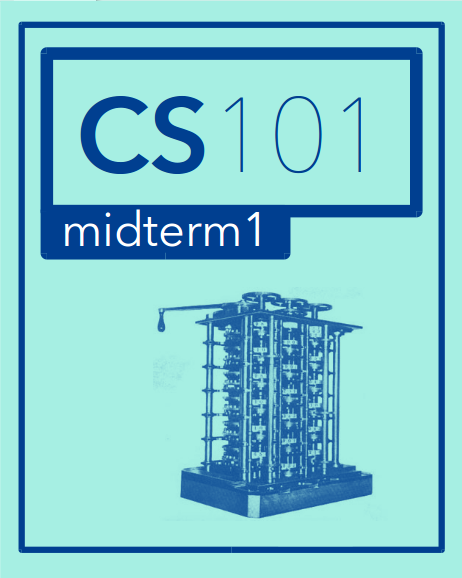
\includegraphics[width=2in]{../img/midterm1-header.png}
\end{center}

\bigskip
\noindent
\begin{itemize}
\item \textbf{Be sure to enter your \underline{NetID} and \underline{the code below} on your Scantron}.
\item Do not turn this page until instructed to do so.
\item There are 30 questions, worth 1 point each.
\item Each question has only \textbf{one} correct answer.
\item You must not communicate with other students during this test.
\item No books, notes, or electronic devices are permitted.
\item This is a 60-minute exam.
\item There are several different versions of this exam.
\end{itemize}

\bigskip\bigskip
\noindent
\textbf{\Large 1. Fill in your information:}

\bigskip
{\Large\bf
\begin{tabular}{ll}
Full Name: & \underbar{\hskip 8cm} \\[0.5em]
UIN (Student Number): & \underbar{\hskip 8cm} \\[0.5em]
NetID: & \underbar{\hskip 8cm}
\end{tabular}
}

\bigskip
\bigskip
\noindent
\textbf{\Large 2. Fill in the following answers on the Scantron form:}

%%%%%%%%%%%%%%%%%%%%%%%%%%%%%%%%%%%%%%%%%%%%%%%%%%%%%%%%%
%%%%%%%%%%%%%%%%%%%%%%%%%%%%%%%%%%%%%%%%%%%%%%%%%%%%%%%%%

\begin{enumerate}
\item[92.] B
\item[93.] E
\item[94.] A
\item[95.] D
\item[96.] B
\end{enumerate}

\newpage

% Zone 1


%%%%%%%%%%%%%%%%%%%%%%%%%%%%%%%%%%%%%%%%%%%%%%%%%%%%%%%%%



\newpage
\noindent
1. (1 point)
Evaluate the following expression:
\begin{verbatim}
[1,2]+[len("3")]
\end{verbatim}
What value is produced?


\begin{enumerate}
\item[(A)] $\bigstar$ 
\begin{verbatim}[1,2,1]\end{verbatim}

\item[(B)]
\begin{verbatim}[1,2,3]\end{verbatim}

\item[(C)]
\begin{verbatim}[1,2,1,2,1,2]\end{verbatim}

\item[(D)]
\begin{verbatim}[1,2,"3"]\end{verbatim}

\end{enumerate}

\vspace*{2em}
\hrule
\vspace{2em}

\noindent {\bf Solution.} 
\vspace{2em}
\hrule height 2pt


\newpage
\noindent
2. (1 point)
Consider the following program:
\begin{verbatim}
x=str("1"*3)
\end{verbatim}
What is the \textbf{value} of \texttt{x} after this program is executed?


\begin{enumerate}
\item[(A)]
\begin{verbatim}3\end{verbatim}

\item[(B)]
None of the other answers are correct.

\item[(C)]
\begin{verbatim}"3"\end{verbatim}

\item[(D)]
\begin{verbatim}111\end{verbatim}

\item[(E)] $\bigstar$ 
\begin{verbatim}"111"\end{verbatim}

\end{enumerate}

\vspace*{2em}
\hrule
\vspace{2em}

\noindent {\bf Solution.} 
\vspace{2em}
\hrule height 2pt


\newpage
\noindent
3. (1 point)
Consider the following program:
\begin{verbatim}
s="Calvin"
i=0
x=-1
while i<len(s):
    if s[i]=='b':
        x=i
    i+=1
\end{verbatim}
What is the \textbf{value} of \texttt{x} after this program is executed?


\begin{enumerate}
\item[(A)]
\begin{verbatim}5\end{verbatim}

\item[(B)]
\begin{verbatim}6\end{verbatim}

\item[(C)] $\bigstar$ 
\begin{verbatim}-1\end{verbatim}

\item[(D)]
\begin{verbatim}3\end{verbatim}

\item[(E)]
\begin{verbatim}0\end{verbatim}

\end{enumerate}

\vspace*{2em}
\hrule
\vspace{2em}

\noindent {\bf Solution.} 
\vspace{2em}
\hrule height 2pt


\newpage
\noindent
4. (1 point)
Consider the following program:
\begin{verbatim}
x=2
a=6
if (a%3)==2:
    x=x**3
elif(a%3)==1:
    x=x**2
else:
    x=x**1
\end{verbatim}
What is the \textbf{value} of \texttt{x} after this program is executed?


\begin{enumerate}
\item[(A)]
\begin{verbatim}16\end{verbatim}

\item[(B)]
\begin{verbatim}8\end{verbatim}

\item[(C)]
None of the other answers are correct.

\item[(D)] $\bigstar$ 
\begin{verbatim}2\end{verbatim}

\item[(E)]
\begin{verbatim}4\end{verbatim}

\end{enumerate}

\vspace*{2em}
\hrule
\vspace{2em}

\noindent {\bf Solution.} 
\vspace{2em}
\hrule height 2pt


\newpage
\noindent
5. (1 point)
Consider the following incomplete function.
\begin{verbatim}
def ismultiple(m,n):
    if ???:
        return False
    else:
        return True
\end{verbatim}
The function is intended to return True if the input parameter m is a multiple of parameter n and False otherwise. For example, \verb|ismultiple(4,2)| should return \verb|True|, but \verb|ismultiple(5,3)| should return \verb|False|. What should replace the three question marks to complete the function?


\begin{enumerate}
\item[(A)]
\begin{verbatim}(n // m) == 0 \end{verbatim}

\item[(B)] $\bigstar$ 
\begin{verbatim}(m % n) != 0 \end{verbatim}

\item[(C)]
\begin{verbatim}(n % m) == 0 \end{verbatim}

\item[(D)]
\begin{verbatim}(m // n) != 0 \end{verbatim}

\end{enumerate}

\vspace*{2em}
\hrule
\vspace{2em}

\noindent {\bf Solution.} 
\vspace{2em}
\hrule height 2pt


\newpage
\noindent
6. (1 point)
Consider the following incomplete Python program.
\begin{verbatim}
s="".join(["1","0","2","1"])
x=0
for i in range(len(s)-1):
    x+=int(???)
\end{verbatim}
What should replace the three question marks so the resulting value of \texttt{x} is 33?


\begin{enumerate}
\item[(A)] $\bigstar$ 
\begin{verbatim}s[i:i+2]\end{verbatim}

\item[(B)]
\begin{verbatim}s[i:i-1]\end{verbatim}

\item[(C)]
\begin{verbatim}s[i+1:i+2]\end{verbatim}

\item[(D)]
\begin{verbatim}s[i:i+1]\end{verbatim}

\end{enumerate}

\vspace*{2em}
\hrule
\vspace{2em}

\noindent {\bf Solution.} 
\vspace{2em}
\hrule height 2pt


\newpage
\noindent
7. (1 point)
Consider the following program:
\begin{verbatim}
a=["merlin","sir agravaine","king pellinore"]
b=[ ]
for i in range(0,3):
    b.append(a[0-i].title())
\end{verbatim}
What is the \textbf{value} of b after this program is executed?


\begin{enumerate}
\item[(A)]
\begin{verbatim}[ ]\end{verbatim}

\item[(B)] $\bigstar$ 
\begin{verbatim}['Merlin', 'King Pellinore', 'Sir Agravaine']\end{verbatim}

\item[(C)]
\begin{verbatim}['Sir Agravaine', 'King Pellinore']\end{verbatim}

\item[(D)]
\begin{verbatim}['King Pellinore', 'Sir Agravaine']\end{verbatim}

\item[(E)]
\begin{verbatim}['King Pellinore', 'Sir Agravaine', 'Merlin']\end{verbatim}

\end{enumerate}

\vspace*{2em}
\hrule
\vspace{2em}

\noindent {\bf Solution.} 
\vspace{2em}
\hrule height 2pt


\newpage
\noindent
8. (1 point)
Consider the following Python program.
\begin{verbatim}
e=[1,3,5,7,9,11]
d=[0,0,0]
for i in range(0,len(e)):
    d[i%3]+=e[i]
x=d[1]
\end{verbatim}
After it is run, what is the final \textbf{value} of \texttt{x}?


\begin{enumerate}
\item[(A)]
\begin{verbatim}0\end{verbatim}

\item[(B)]
\begin{verbatim}16\end{verbatim}

\item[(C)]
\begin{verbatim}8\end{verbatim}

\item[(D)] $\bigstar$ 
\begin{verbatim}12\end{verbatim}

\item[(E)]
\begin{verbatim}3\end{verbatim}

\end{enumerate}

\vspace*{2em}
\hrule
\vspace{2em}

\noindent {\bf Solution.} 
\vspace{2em}
\hrule height 2pt


\newpage
\noindent
9. (1 point)
How can the following mathematical equation be implemented as a Python expression? Assume \verb|a|, \verb|b|, and \verb|cos| have already been defined.
$$a^b \cos(a - b)$$


\begin{enumerate}
\item[(A)]
None of the other answers are correct.

\item[(B)]
\begin{verbatim}(b^a)cos(a-b)\end{verbatim}

\item[(C)]
\begin{verbatim}(a**b)cos(a-b)\end{verbatim}

\item[(D)] $\bigstar$ 
\begin{verbatim}(a**b)*cos(a-b)\end{verbatim}

\item[(E)]
\begin{verbatim}(a^b)*cos(a-b)\end{verbatim}

\end{enumerate}

\vspace*{2em}
\hrule
\vspace{2em}

\noindent {\bf Solution.} 
\vspace{2em}
\hrule height 2pt


\newpage
\noindent
10. (1 point)
Consider the following program:
\begin{verbatim}
a=3
b=4
if a==3:
    b=a
elif a==4:
    a=5
else:
    a=b
\end{verbatim}
What is the \textbf{value} of a after this program is executed?


\begin{enumerate}
\item[(A)]
None of the other answers are correct.

\item[(B)] $\bigstar$ 
\begin{verbatim}3\end{verbatim}

\item[(C)]
\begin{verbatim}7\end{verbatim}

\item[(D)]
\begin{verbatim}5\end{verbatim}

\item[(E)]
\begin{verbatim}4\end{verbatim}

\end{enumerate}

\vspace*{2em}
\hrule
\vspace{2em}

\noindent {\bf Solution.} 
\vspace{2em}
\hrule height 2pt


\newpage
\noindent
11. (1 point)
Consider the following program:
\begin{verbatim}
x=[2,3,4,5,6,7,8,9]
x=x[2:-2]
i=1
while i <= 3:
    x[i]+=1
    i+=1
\end{verbatim}
What is the \textbf{value} of \texttt{x} after this program is executed?


\begin{enumerate}
\item[(A)]
\begin{verbatim}[4, 6, 7]\end{verbatim}

\item[(B)]
\begin{verbatim}[2, 4, 6, 6]\end{verbatim}

\item[(C)]
\begin{verbatim}[3, 4, 6, 7, 8]\end{verbatim}

\item[(D)] $\bigstar$ 
\begin{verbatim}[4, 6, 7, 8]\end{verbatim}

\item[(E)]
\begin{verbatim}[4, 6, 7, 7]\end{verbatim}

\end{enumerate}

\vspace*{2em}
\hrule
\vspace{2em}

\noindent {\bf Solution.} 
\vspace{2em}
\hrule height 2pt


\newpage
\noindent
12. (1 point)
Consider the following program.
\begin{verbatim}
x=1
i=0
while(x*x)<=9:
    i=i+(x*x)
    x=x+1
\end{verbatim}
After it is run, what is the final \textbf{value} of \texttt{x}?


\begin{enumerate}
\item[(A)]
\begin{verbatim}30\end{verbatim}

\item[(B)]
\begin{verbatim}3\end{verbatim}

\item[(C)]
\begin{verbatim}14\end{verbatim}

\item[(D)]
\begin{verbatim}5\end{verbatim}

\item[(E)] $\bigstar$ 
\begin{verbatim}4\end{verbatim}

\end{enumerate}

\vspace*{2em}
\hrule
\vspace{2em}

\noindent {\bf Solution.} 
\vspace{2em}
\hrule height 2pt


\newpage
\noindent
13. (1 point)
Consider the following program:
\begin{verbatim}
x="KING ARTHUR-MORGANA LEFAY-SIR BEDIVERE".split("-")
y=x[:]
y.reverse()
\end{verbatim}
What is the \textbf{value} of \texttt{x} after this program is executed?


\begin{enumerate}
\item[(A)]
\begin{verbatim}['BEDIVERE', 'LEFAY-SIR', 'ARTHUR-MORGANA', 'KING']\end{verbatim}

\item[(B)] $\bigstar$ 
\begin{verbatim}['KING ARTHUR', 'MORGANA LEFAY', 'SIR BEDIVERE']\end{verbatim}

\item[(C)]
\begin{verbatim}['KING', 'ARTHUR-MORGANA', 'LEFAY-SIR', 'BEDIVERE']\end{verbatim}

\item[(D)]
\begin{verbatim}['SIR BEDIVERE', 'MORGANA LEFAY', 'KING ARTHUR']\end{verbatim}

\item[(E)]
\begin{verbatim}None\end{verbatim}

\end{enumerate}

\vspace*{2em}
\hrule
\vspace{2em}

\noindent {\bf Solution.} 
\vspace{2em}
\hrule height 2pt


\newpage
\noindent
14. (1 point)
Consider the following program.
\begin{verbatim}
def artificing(s):
    return s*2
    return s+"%i" % 2
    return s

s=artificing("MERLIN")
\end{verbatim}
After it is run, what is the final \textbf{value} of s?


\begin{enumerate}
\item[(A)] $\bigstar$ 
\begin{verbatim}"MERLINMERLIN"\end{verbatim}

\item[(B)]
\begin{verbatim}"MERLIN2"\end{verbatim}

\item[(C)]
\begin{verbatim}"MERLIN"\end{verbatim}

\item[(D)]
\begin{verbatim}None\end{verbatim}

\item[(E)]
\begin{verbatim}12\end{verbatim}

\end{enumerate}

\vspace*{2em}
\hrule
\vspace{2em}

\noindent {\bf Solution.} 
\vspace{2em}
\hrule height 2pt


\newpage
\noindent
15. (1 point)
Consider the following program:
\begin{verbatim}
x=0
for i in range(2,7):
    if i%3==0:
        x+=3
    elif i%2==0:
        x+=2
    else:
        x+=1
\end{verbatim}
What is the \textbf{value} of \texttt{x} after this program is executed?


\begin{enumerate}
\item[(A)]
\begin{verbatim}13\end{verbatim}

\item[(B)] $\bigstar$ 
\begin{verbatim}11\end{verbatim}

\item[(C)]
\begin{verbatim}12\end{verbatim}

\item[(D)]
\begin{verbatim}10\end{verbatim}

\item[(E)]
\begin{verbatim}14\end{verbatim}

\end{enumerate}

\vspace*{2em}
\hrule
\vspace{2em}

\noindent {\bf Solution.} 
\vspace{2em}
\hrule height 2pt


\newpage
\noindent
16. (1 point)
Consider the following program:
\begin{verbatim}
s="ECTOR"
t="GAWAIN"
x=(len(s)+len(t)) < 4 and s in t
\end{verbatim}
What is the \textbf{type} of \texttt{x} after this program is executed?


\begin{enumerate}
\item[(A)] $\bigstar$ 
\begin{verbatim}Boolean\end{verbatim}

\item[(B)]
\begin{verbatim}None\end{verbatim}

\item[(C)]
\begin{verbatim}Integer\end{verbatim}

\item[(D)]
\begin{verbatim}Float\end{verbatim}

\item[(E)]
\begin{verbatim}String\end{verbatim}

\end{enumerate}

\vspace*{2em}
\hrule
\vspace{2em}

\noindent {\bf Solution.} 
\vspace{2em}
\hrule height 2pt


\newpage
\noindent
17. (1 point)
Consider the following program:
\begin{verbatim}
i=3
x=2
while i < 7:
    x+=i
    i+=2
\end{verbatim}
What is the \textbf{value} of \texttt{x} after this program is executed?


\begin{enumerate}
\item[(A)]
\begin{verbatim}14\end{verbatim}

\item[(B)]
\begin{verbatim}13\end{verbatim}

\item[(C)] $\bigstar$ 
\begin{verbatim}10\end{verbatim}

\item[(D)]
\begin{verbatim}11\end{verbatim}

\item[(E)]
\begin{verbatim}12\end{verbatim}

\end{enumerate}

\vspace*{2em}
\hrule
\vspace{2em}

\noindent {\bf Solution.} 
\vspace{2em}
\hrule height 2pt


\newpage
\noindent
18. (1 point)
For this problem, you should compose a function which accomplishes a given task using the available code blocks arranged in the correct functional order.  \emph{We ignore indentation for this problem.}

\texttt{find\_max} should accept a \texttt{list} and return the value of the maximum item in the \texttt{list}.  (\texttt{None} is always the lowest value in any numeric comparison, so you may use it as an initializer.)

\begin{verbatim}
def find_max(my_list):
\end{verbatim}

\begin{enumerate}[1]
\item \texttt{max\_val = i}
\item \texttt{max\_val = None}
\item \texttt{for i in range(len(my\_list)):}
\item \texttt{if i > max\_val:}
\item \texttt{max\_val = my\_list[i]}
\item \texttt{return max\_val}
\item \texttt{for i in range(my\_list):}
\item \texttt{if my\_list[i] > max\_val:}
\item \texttt{print(max\_val)}
\end{enumerate}



\begin{enumerate}
\item[(A)]
2, 3, 4, 1, 6

\item[(B)]
2, 3, 8, 1, 6

\item[(C)]
2, 7, 4, 5, 6

\item[(D)]
3, 2, 8, 5, 9

\item[(E)] $\bigstar$ 
2, 3, 8, 5, 6

\end{enumerate}

\vspace*{2em}
\hrule
\vspace{2em}

\noindent {\bf Solution.} 
\vspace{2em}
\hrule height 2pt


\newpage
\noindent
19. (1 point)
Consider the following program:
\begin{verbatim}
x=[1,2,3]
def f(a):
    s=""
    a.append(4)
    for i in a:
        s+=str(i)
    return s

x.append(f(x))
\end{verbatim}
What is the \textbf{value} of \texttt{x} after this program is executed?


\begin{enumerate}
\item[(A)]
\begin{verbatim}[1, 2, 3, 10]\end{verbatim}

\item[(B)]
\begin{verbatim}[1, 2, 3]\end{verbatim}

\item[(C)] $\bigstar$ 
\begin{verbatim}[1, 2, 3, 4, '1234']\end{verbatim}

\item[(D)]
\begin{verbatim}[1, 2, 3, '1234']\end{verbatim}

\item[(E)]
\begin{verbatim}[1, 2, 3, '123']\end{verbatim}

\end{enumerate}

\vspace*{2em}
\hrule
\vspace{2em}

\noindent {\bf Solution.} 
\vspace{2em}
\hrule height 2pt


\newpage
\noindent
20. (1 point)
Consider the following program:
\begin{verbatim}
s="TRIS %i"
t="ISEU"
x=s % len(t)
\end{verbatim}
What is the \textbf{type} of \texttt{x} after this program is executed?


\begin{enumerate}
\item[(A)] $\bigstar$ 
\begin{verbatim}String\end{verbatim}

\item[(B)]
\begin{verbatim}Float\end{verbatim}

\item[(C)]
\begin{verbatim}Boolean\end{verbatim}

\item[(D)]
\begin{verbatim}Integer\end{verbatim}

\item[(E)]
\begin{verbatim}None\end{verbatim}

\end{enumerate}

\vspace*{2em}
\hrule
\vspace{2em}

\noindent {\bf Solution.} 
\vspace{2em}
\hrule height 2pt


\newpage
\noindent
21. (1 point)
Consider the following program:
\begin{verbatim}
pi="3.14159"
e="2.71828"
x=(float(e)**float(pi)-float(pi)) == 20
\end{verbatim}
What is the \textbf{type} of \texttt{x} after this program is executed?


\begin{enumerate}
\item[(A)]
\begin{verbatim}None\end{verbatim}

\item[(B)] $\bigstar$ 
\begin{verbatim}Boolean\end{verbatim}

\item[(C)]
\begin{verbatim}Integer\end{verbatim}

\item[(D)]
\begin{verbatim}Float\end{verbatim}

\item[(E)]
\begin{verbatim}String\end{verbatim}

\end{enumerate}

\vspace*{2em}
\hrule
\vspace{2em}

\noindent {\bf Solution.} 
\vspace{2em}
\hrule height 2pt


\newpage
\noindent
22. (1 point)
What is the result of the following expression?
\begin{verbatim}
[ 1, 2, 3 ] * 3
\end{verbatim}


\begin{enumerate}
\item[(A)] $\bigstar$ 
\begin{verbatim}[1, 2, 3, 1, 2, 3, 1, 2, 3]\end{verbatim}

\item[(B)]
\begin{verbatim}[1.0, 2.0, 3.0, 1.0, 2.0, 3.0, 1.0, 2.0, 3.0]\end{verbatim}

\item[(C)]
\begin{verbatim}[3, 6, 9]\end{verbatim}

\item[(D)]
\begin{verbatim}(3, 6, 9)\end{verbatim}

\item[(E)]
\begin{verbatim}[3.0, 6.0, 9.0]\end{verbatim}

\end{enumerate}

\vspace*{2em}
\hrule
\vspace{2em}

\noindent {\bf Solution.} 
\vspace{2em}
\hrule height 2pt


\newpage
\noindent
23. (1 point)
Consider the following program:
\begin{verbatim}
def fix(s):
    a=list(s)
    a.sort()
    return ''.join(a)

x=["one","two","eleven","twelve"]
s1=fix(x[0]+x[-1])
s2=fix(x[1]+x[-2])

if s1<s2:
    x.sort()
elif s1>s2:
    x.reverse()
else:
    x.append("six")
\end{verbatim}
What is the \textbf{value} of \texttt{x} after this program is executed?


\begin{enumerate}
\item[(A)]
\begin{verbatim}['twelve', 'eleven', 'two', 'one']\end{verbatim}

\item[(B)] $\bigstar$ 
\begin{verbatim}['one', 'two', 'eleven', 'twelve', 'six']\end{verbatim}

\item[(C)]
\begin{verbatim}['eleven', 'one', 'twelve', 'two']\end{verbatim}

\item[(D)]
\begin{verbatim}['two', 'twelve', 'one', 'eleven', 'six']\end{verbatim}

\item[(E)]
\begin{verbatim}['one', 'two', 'eleven', 'twelve']\end{verbatim}

\end{enumerate}

\vspace*{2em}
\hrule
\vspace{2em}

\noindent {\bf Solution.} 
\vspace{2em}
\hrule height 2pt


\newpage
\noindent
24. (1 point)
Consider the following program:
\begin{verbatim}
s="G+R+A+I+L"
x=s.split("+")[1:-2]
\end{verbatim}
What is the \textbf{value} of \texttt{x} after this program is executed?


\begin{enumerate}
\item[(A)]
\begin{verbatim}None\end{verbatim}

\item[(B)]
\begin{verbatim}False\end{verbatim}

\item[(C)]
\begin{verbatim}'RAI'\end{verbatim}

\item[(D)] $\bigstar$ 
\begin{verbatim}['R','A']\end{verbatim}

\item[(E)]
\begin{verbatim}3\end{verbatim}

\end{enumerate}

\vspace*{2em}
\hrule
\vspace{2em}

\noindent {\bf Solution.} 
\vspace{2em}
\hrule height 2pt


\newpage
\noindent
25. (1 point)
Consider the following program:
\begin{verbatim}
a=["A","C","C","I","O"]
a.sort()
a[0]=a[-1]
x=""
for e in a:
    x=x+e
\end{verbatim}
What is the \textbf{value} of \texttt{x} after this program is executed?


\begin{enumerate}
\item[(A)]
\begin{verbatim}"ICCOI"\end{verbatim}

\item[(B)]
None of the other answers are correct.

\item[(C)]
\begin{verbatim}"ACCIA"\end{verbatim}

\item[(D)]
\begin{verbatim}"ACCOA"\end{verbatim}

\item[(E)] $\bigstar$ 
\begin{verbatim}"OCCIO"\end{verbatim}

\end{enumerate}

\vspace*{2em}
\hrule
\vspace{2em}

\noindent {\bf Solution.} 
\vspace{2em}
\hrule height 2pt


\newpage
\noindent
26. (1 point)
Evaluate the following expression:
\begin{verbatim}
len("ABCD"[0:3])
\end{verbatim}
What value is produced?


\begin{enumerate}
\item[(A)]
1

\item[(B)]
2

\item[(C)] $\bigstar$ 
3

\item[(D)]
4

\end{enumerate}

\vspace*{2em}
\hrule
\vspace{2em}

\noindent {\bf Solution.} 
\vspace{2em}
\hrule height 2pt


\newpage
\noindent
27. (1 point)
Consider the following program.
\begin{verbatim}
kay = 2
wart = 3

def knight(kay,wart):
    wart += 2
    kay += 3
    return wart + kay

wart = knight(kay, kay) + knight(wart, wart)
\end{verbatim}
After it is run, what is the final \textbf{value} of \texttt{wart}?


\begin{enumerate}
\item[(A)]
\begin{verbatim}3\end{verbatim}

\item[(B)] $\bigstar$ 
None of the other answers are correct.

\item[(C)]
\begin{verbatim}2\end{verbatim}

\item[(D)]
\begin{verbatim}5\end{verbatim}

\end{enumerate}

\vspace*{2em}
\hrule
\vspace{2em}

\noindent {\bf Solution.} 
\vspace{2em}
\hrule height 2pt


\newpage
\noindent
28. (1 point)
Consider the following program.
\begin{verbatim}
s="ABCBA"
x=0
y=len(s)-1
while s[x]==s[y] and x<y:
    x+=1
    y-=1
\end{verbatim}
After it is run, what is the final \textbf{value} of \texttt{x}?


\begin{enumerate}
\item[(A)]
\begin{verbatim}3\end{verbatim}

\item[(B)]
\begin{verbatim}1\end{verbatim}

\item[(C)]
\begin{verbatim}0\end{verbatim}

\item[(D)] $\bigstar$ 
\begin{verbatim}2\end{verbatim}

\item[(E)]
\begin{verbatim}4\end{verbatim}

\end{enumerate}

\vspace*{2em}
\hrule
\vspace{2em}

\noindent {\bf Solution.} 
\vspace{2em}
\hrule height 2pt


\newpage
\noindent
29. (1 point)
Consider the following program.
\begin{verbatim}
x=[]
for j in range(0,5):
    if (j%3)==0:
        x.append("-")
    if (j%4)==0:
        x.append("*")
\end{verbatim}
After it is run, what is the final \textbf{value} of \texttt{x}?


\begin{enumerate}
\item[(A)]
\begin{verbatim}["*","-","*"]\end{verbatim}

\item[(B)]
\begin{verbatim}["-","*"]\end{verbatim}

\item[(C)]
None of the other answers are correct.

\item[(D)] $\bigstar$ 
\begin{verbatim}["-","*","-","*"]\end{verbatim}

\item[(E)]
\begin{verbatim}["*","-","*"]\end{verbatim}

\end{enumerate}

\vspace*{2em}
\hrule
\vspace{2em}

\noindent {\bf Solution.} 
\vspace{2em}
\hrule height 2pt


\newpage
\noindent
30. (1 point)
Consider the following incomplete program.
\begin{verbatim}
sum=0
???:
    sum=sum+i

\end{verbatim}
The program is intended to sum all of the integers between 1 and 100 (inclusive). What should replace the three question marks to complete the program?


\begin{enumerate}
\item[(A)]
\begin{verbatim}while i in range(100)\end{verbatim}

\item[(B)] $\bigstar$ 
\begin{verbatim}for i in range(1,101) \end{verbatim}

\item[(C)]
\begin{verbatim}while i<=100 \end{verbatim}

\item[(D)]
\begin{verbatim}for i in range(0,100)\end{verbatim}

\end{enumerate}

\vspace*{2em}
\hrule
\vspace{2em}

\noindent {\bf Solution.} 
\vspace{2em}
\hrule height 2pt

%%%%%%%%%%%%%%%%%%%%%%%%%%%%%%%%%%%%%%%%%%%%%%%%%%%%%%%%%%%%%%%%%%%%%%
%%%%%%%%%%%%%%%%%%%%%%%%%%%%%%%%%%%%%%%%%%%%%%%%%%%%%%%%%%%%%%%%%%%%%%
%%%%%%%%%%%%%%%%%%%%%%%%%%%%%%%%%%%%%%%%%%%%%%%%%%%%%%%%%%%%%%%%%%%%%%
%%%%%%%%%%%%%%%%%%%%%%%%%%%%%%%%%%%%%%%%%%%%%%%%%%%%%%%%%%%%%%%%%%%%%%
% Exam number 23

\message{Exam 23/50}
\cleardoublepage
\setcounter{page}{1}


\begin{center}
%\textbf{\Large CS 101 Midterm \#1}
%
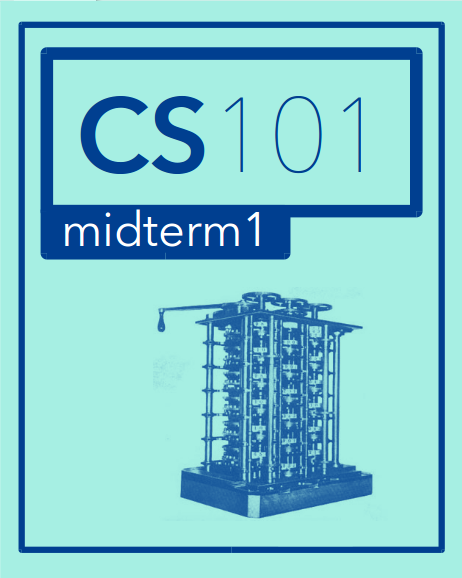
\includegraphics[width=2in]{../img/midterm1-header.png}
\end{center}

\bigskip
\noindent
\begin{itemize}
\item \textbf{Be sure to enter your \underline{NetID} and \underline{the code below} on your Scantron}.
\item Do not turn this page until instructed to do so.
\item There are 30 questions, worth 1 point each.
\item Each question has only \textbf{one} correct answer.
\item You must not communicate with other students during this test.
\item No books, notes, or electronic devices are permitted.
\item This is a 60-minute exam.
\item There are several different versions of this exam.
\end{itemize}

\bigskip\bigskip
\noindent
\textbf{\Large 1. Fill in your information:}

\bigskip
{\Large\bf
\begin{tabular}{ll}
Full Name: & \underbar{\hskip 8cm} \\[0.5em]
UIN (Student Number): & \underbar{\hskip 8cm} \\[0.5em]
NetID: & \underbar{\hskip 8cm}
\end{tabular}
}

\bigskip
\bigskip
\noindent
\textbf{\Large 2. Fill in the following answers on the Scantron form:}

%%%%%%%%%%%%%%%%%%%%%%%%%%%%%%%%%%%%%%%%%%%%%%%%%%%%%%%%%
%%%%%%%%%%%%%%%%%%%%%%%%%%%%%%%%%%%%%%%%%%%%%%%%%%%%%%%%%

\begin{enumerate}
\item[92.] C
\item[93.] E
\item[94.] A
\item[95.] E
\item[96.] C
\end{enumerate}

\newpage

% Zone 1


%%%%%%%%%%%%%%%%%%%%%%%%%%%%%%%%%%%%%%%%%%%%%%%%%%%%%%%%%



\newpage
\noindent
1. (1 point)
Consider the following program:
\begin{verbatim}
pi="3.14159"
e="2.71828"
x=(float(e)**float(pi)-float(pi)) == 20
\end{verbatim}
What is the \textbf{type} of \texttt{x} after this program is executed?


\begin{enumerate}
\item[(A)]
\begin{verbatim}Integer\end{verbatim}

\item[(B)] $\bigstar$ 
\begin{verbatim}Boolean\end{verbatim}

\item[(C)]
\begin{verbatim}None\end{verbatim}

\item[(D)]
\begin{verbatim}String\end{verbatim}

\item[(E)]
\begin{verbatim}Float\end{verbatim}

\end{enumerate}

\vspace*{2em}
\hrule
\vspace{2em}

\noindent {\bf Solution.} 
\vspace{2em}
\hrule height 2pt


\newpage
\noindent
2. (1 point)
Consider the following program:
\begin{verbatim}
s="ECTOR"
t="GAWAIN"
x=(len(s)+len(t)) < 4 and s in t
\end{verbatim}
What is the \textbf{type} of \texttt{x} after this program is executed?


\begin{enumerate}
\item[(A)]
\begin{verbatim}None\end{verbatim}

\item[(B)]
\begin{verbatim}Integer\end{verbatim}

\item[(C)]
\begin{verbatim}String\end{verbatim}

\item[(D)]
\begin{verbatim}Float\end{verbatim}

\item[(E)] $\bigstar$ 
\begin{verbatim}Boolean\end{verbatim}

\end{enumerate}

\vspace*{2em}
\hrule
\vspace{2em}

\noindent {\bf Solution.} 
\vspace{2em}
\hrule height 2pt


\newpage
\noindent
3. (1 point)
Consider the following program.
\begin{verbatim}
x=1
i=0
while(x*x)<=9:
    i=i+(x*x)
    x=x+1
\end{verbatim}
After it is run, what is the final \textbf{value} of \texttt{x}?


\begin{enumerate}
\item[(A)]
\begin{verbatim}3\end{verbatim}

\item[(B)] $\bigstar$ 
\begin{verbatim}4\end{verbatim}

\item[(C)]
\begin{verbatim}5\end{verbatim}

\item[(D)]
\begin{verbatim}30\end{verbatim}

\item[(E)]
\begin{verbatim}14\end{verbatim}

\end{enumerate}

\vspace*{2em}
\hrule
\vspace{2em}

\noindent {\bf Solution.} 
\vspace{2em}
\hrule height 2pt


\newpage
\noindent
4. (1 point)
Consider the following program.
\begin{verbatim}
def artificing(s):
    return s*2
    return s+"%i" % 2
    return s

s=artificing("MERLIN")
\end{verbatim}
After it is run, what is the final \textbf{value} of s?


\begin{enumerate}
\item[(A)]
\begin{verbatim}12\end{verbatim}

\item[(B)]
\begin{verbatim}"MERLIN2"\end{verbatim}

\item[(C)]
\begin{verbatim}"MERLIN"\end{verbatim}

\item[(D)] $\bigstar$ 
\begin{verbatim}"MERLINMERLIN"\end{verbatim}

\item[(E)]
\begin{verbatim}None\end{verbatim}

\end{enumerate}

\vspace*{2em}
\hrule
\vspace{2em}

\noindent {\bf Solution.} 
\vspace{2em}
\hrule height 2pt


\newpage
\noindent
5. (1 point)
Consider the following program:
\begin{verbatim}
x=str("1"*3)
\end{verbatim}
What is the \textbf{value} of \texttt{x} after this program is executed?


\begin{enumerate}
\item[(A)]
\begin{verbatim}111\end{verbatim}

\item[(B)]
\begin{verbatim}3\end{verbatim}

\item[(C)] $\bigstar$ 
\begin{verbatim}"111"\end{verbatim}

\item[(D)]
None of the other answers are correct.

\item[(E)]
\begin{verbatim}"3"\end{verbatim}

\end{enumerate}

\vspace*{2em}
\hrule
\vspace{2em}

\noindent {\bf Solution.} 
\vspace{2em}
\hrule height 2pt


\newpage
\noindent
6. (1 point)
Consider the following program:
\begin{verbatim}
s="Calvin"
i=0
x=-1
while i<len(s):
    if s[i]=='b':
        x=i
    i+=1
\end{verbatim}
What is the \textbf{value} of \texttt{x} after this program is executed?


\begin{enumerate}
\item[(A)] $\bigstar$ 
\begin{verbatim}-1\end{verbatim}

\item[(B)]
\begin{verbatim}5\end{verbatim}

\item[(C)]
\begin{verbatim}0\end{verbatim}

\item[(D)]
\begin{verbatim}6\end{verbatim}

\item[(E)]
\begin{verbatim}3\end{verbatim}

\end{enumerate}

\vspace*{2em}
\hrule
\vspace{2em}

\noindent {\bf Solution.} 
\vspace{2em}
\hrule height 2pt


\newpage
\noindent
7. (1 point)
Consider the following program:
\begin{verbatim}
s="TRIS %i"
t="ISEU"
x=len(s) % len(t[2:-1])
\end{verbatim}
What is the \textbf{type} of \texttt{x} after this program is executed?


\begin{enumerate}
\item[(A)]
\begin{verbatim}Boolean\end{verbatim}

\item[(B)]
\begin{verbatim}Float\end{verbatim}

\item[(C)]
\begin{verbatim}String\end{verbatim}

\item[(D)]
\begin{verbatim}None\end{verbatim}

\item[(E)] $\bigstar$ 
\begin{verbatim}Integer\end{verbatim}

\end{enumerate}

\vspace*{2em}
\hrule
\vspace{2em}

\noindent {\bf Solution.} 
\vspace{2em}
\hrule height 2pt


\newpage
\noindent
8. (1 point)
Consider the following program:
\begin{verbatim}
a=3
b=4
if a==3:
    a=b
elif a==4:
    a=5
else:
    b=a
\end{verbatim}
What is the \textbf{value} of a after this program is executed?


\begin{enumerate}
\item[(A)]
None of the other answers are correct.

\item[(B)]
\begin{verbatim}3\end{verbatim}

\item[(C)] $\bigstar$ 
\begin{verbatim}4\end{verbatim}

\item[(D)]
\begin{verbatim}5\end{verbatim}

\item[(E)]
\begin{verbatim}7\end{verbatim}

\end{enumerate}

\vspace*{2em}
\hrule
\vspace{2em}

\noindent {\bf Solution.} 
\vspace{2em}
\hrule height 2pt


\newpage
\noindent
9. (1 point)
How can the following mathematical equation be implemented as a Python expression? Assume \verb|a|, \verb|b|, and \verb|cos| have already been defined.
$$a^b \cos(a - b)$$


\begin{enumerate}
\item[(A)]
\begin{verbatim}(a^b)*cos(a-b)\end{verbatim}

\item[(B)]
None of the other answers are correct.

\item[(C)] $\bigstar$ 
\begin{verbatim}(a**b)*cos(a-b)\end{verbatim}

\item[(D)]
\begin{verbatim}(a**b)cos(a-b)\end{verbatim}

\item[(E)]
\begin{verbatim}(b^a)cos(a-b)\end{verbatim}

\end{enumerate}

\vspace*{2em}
\hrule
\vspace{2em}

\noindent {\bf Solution.} 
\vspace{2em}
\hrule height 2pt


\newpage
\noindent
10. (1 point)
Consider the following program:
\begin{verbatim}
x=3
a=7
if (a%3)==2:
    x=x**2
elif(a%3)==1:
    x=x**1
else:
    x=x**0
\end{verbatim}
What is the \textbf{value} of \texttt{x} after this program is executed?


\begin{enumerate}
\item[(A)]
\begin{verbatim}1\end{verbatim}

\item[(B)]
\begin{verbatim}9\end{verbatim}

\item[(C)]
None of the other answers are correct.

\item[(D)] $\bigstar$ 
\begin{verbatim}3\end{verbatim}

\item[(E)]
\begin{verbatim}7\end{verbatim}

\end{enumerate}

\vspace*{2em}
\hrule
\vspace{2em}

\noindent {\bf Solution.} 
\vspace{2em}
\hrule height 2pt


\newpage
\noindent
11. (1 point)
Consider the following program:
\begin{verbatim}
x=[1,2,3]
def f(a):
    s=""
    a.append(4)
    for i in a:
        s+=str(i)
    return s

x.append(f(x))
\end{verbatim}
What is the \textbf{value} of \texttt{x} after this program is executed?


\begin{enumerate}
\item[(A)]
\begin{verbatim}[1, 2, 3, '123']\end{verbatim}

\item[(B)]
\begin{verbatim}[1, 2, 3]\end{verbatim}

\item[(C)]
\begin{verbatim}[1, 2, 3, '1234']\end{verbatim}

\item[(D)]
\begin{verbatim}[1, 2, 3, 10]\end{verbatim}

\item[(E)] $\bigstar$ 
\begin{verbatim}[1, 2, 3, 4, '1234']\end{verbatim}

\end{enumerate}

\vspace*{2em}
\hrule
\vspace{2em}

\noindent {\bf Solution.} 
\vspace{2em}
\hrule height 2pt


\newpage
\noindent
12. (1 point)
Consider the following program:
\begin{verbatim}
s="-B-O-R-S-"
x=s.split("-")[2:-2]
\end{verbatim}
What is the \textbf{value} of \texttt{x} after this program is executed?


\begin{enumerate}
\item[(A)]
\begin{verbatim}None\end{verbatim}

\item[(B)]
\begin{verbatim}'ORS'\end{verbatim}

\item[(C)] $\bigstar$ 
\begin{verbatim}['O', 'R']\end{verbatim}

\item[(D)]
\begin{verbatim}False\end{verbatim}

\item[(E)]
\begin{verbatim}''\end{verbatim}

\end{enumerate}

\vspace*{2em}
\hrule
\vspace{2em}

\noindent {\bf Solution.} 
\vspace{2em}
\hrule height 2pt


\newpage
\noindent
13. (1 point)
Consider the following program:
\begin{verbatim}
x=[1,2,3,4,5,6,7,8,9]
x=x[2:-2]
i=1
while i <= 3:
    x[i]+=1
    i+=1
\end{verbatim}
What is the \textbf{value} of \texttt{x} after this program is executed?


\begin{enumerate}
\item[(A)] $\bigstar$ 
\begin{verbatim}[3, 5, 6, 7, 7]\end{verbatim}

\item[(B)]
\begin{verbatim}[3, 5, 6, 7, 7, 8]\end{verbatim}

\item[(C)]
\begin{verbatim}[2, 4, 5, 6, 7, 7]\end{verbatim}

\item[(D)]
\begin{verbatim}[2, 4, 5, 5, 7, 7]\end{verbatim}

\item[(E)]
\begin{verbatim}[3, 5, 7, 7]\end{verbatim}

\end{enumerate}

\vspace*{2em}
\hrule
\vspace{2em}

\noindent {\bf Solution.} 
\vspace{2em}
\hrule height 2pt


\newpage
\noindent
14. (1 point)
Consider the following program.
\begin{verbatim}
x=[]
for j in range(0,5):
    if (j%4)==0:
        x.append("-")
    if (j%5)==0:
        x.append("*")
\end{verbatim}
After it is run, what is the final \textbf{value} of \texttt{x}?


\begin{enumerate}
\item[(A)]
\begin{verbatim}["-","*","*"]\end{verbatim}

\item[(B)]
None of the other answers are correct.

\item[(C)] $\bigstar$ 
\begin{verbatim}["-","*","-"]\end{verbatim}

\item[(D)]
\begin{verbatim}["-","*"]\end{verbatim}

\item[(E)]
\begin{verbatim}["-","-","*"]\end{verbatim}

\end{enumerate}

\vspace*{2em}
\hrule
\vspace{2em}

\noindent {\bf Solution.} 
\vspace{2em}
\hrule height 2pt


\newpage
\noindent
15. (1 point)
For this problem, you should compose a function which accomplishes a given task using the available code blocks arranged in the correct functional order.  \emph{We ignore indentation for this problem.}

\texttt{find\_max} should accept a \texttt{list} and return the value of the maximum item in the \texttt{list}.  (\texttt{None} is always the lowest value in any numeric comparison, so you may use it as an initializer.)

\begin{verbatim}
def find_max(my_list):
\end{verbatim}

\begin{enumerate}[1]
\item \texttt{max\_val = i}
\item \texttt{max\_val = None}
\item \texttt{for i in range(len(my\_list)):}
\item \texttt{if i > max\_val:}
\item \texttt{max\_val = my\_list[i]}
\item \texttt{return max\_val}
\item \texttt{for i in range(my\_list):}
\item \texttt{if my\_list[i] > max\_val:}
\item \texttt{print(max\_val)}
\end{enumerate}



\begin{enumerate}
\item[(A)]
2, 3, 4, 1, 6

\item[(B)]
2, 3, 8, 1, 6

\item[(C)]
3, 2, 8, 5, 9

\item[(D)]
2, 7, 4, 5, 6

\item[(E)] $\bigstar$ 
2, 3, 8, 5, 6

\end{enumerate}

\vspace*{2em}
\hrule
\vspace{2em}

\noindent {\bf Solution.} 
\vspace{2em}
\hrule height 2pt


\newpage
\noindent
16. (1 point)
Consider the following incomplete function.
\begin{verbatim}
def ismultiple(m,n):
    if ???:
        return False
    else:
        return True
\end{verbatim}
The function is intended to return True if the input parameter m is a multiple of parameter n and False otherwise. For example, \verb|ismultiple(4,2)| should return \verb|True|, but \verb|ismultiple(5,3)| should return \verb|False|. What should replace the three question marks to complete the function?


\begin{enumerate}
\item[(A)]
\begin{verbatim}(m // n) != 0 \end{verbatim}

\item[(B)]
\begin{verbatim}(n // m) == 0 \end{verbatim}

\item[(C)] $\bigstar$ 
\begin{verbatim}(m % n) != 0 \end{verbatim}

\item[(D)]
\begin{verbatim}(n % m) == 0 \end{verbatim}

\end{enumerate}

\vspace*{2em}
\hrule
\vspace{2em}

\noindent {\bf Solution.} 
\vspace{2em}
\hrule height 2pt


\newpage
\noindent
17. (1 point)
Consider the following program:
\begin{verbatim}
a=["merlin","sir agravaine","king pellinore"]
b=[ ]
for i in range(0,3):
    b.append(a[0-i].title())
\end{verbatim}
What is the \textbf{value} of b after this program is executed?


\begin{enumerate}
\item[(A)]
\begin{verbatim}[ ]\end{verbatim}

\item[(B)]
\begin{verbatim}['Sir Agravaine', 'King Pellinore']\end{verbatim}

\item[(C)]
\begin{verbatim}['King Pellinore', 'Sir Agravaine', 'Merlin']\end{verbatim}

\item[(D)]
\begin{verbatim}['King Pellinore', 'Sir Agravaine']\end{verbatim}

\item[(E)] $\bigstar$ 
\begin{verbatim}['Merlin', 'King Pellinore', 'Sir Agravaine']\end{verbatim}

\end{enumerate}

\vspace*{2em}
\hrule
\vspace{2em}

\noindent {\bf Solution.} 
\vspace{2em}
\hrule height 2pt


\newpage
\noindent
18. (1 point)
Consider the following program:
\begin{verbatim}
x="KING ARTHUR-MORGANA LEFAY-SIR BEDIVERE".split("-")
y=x
x=y.reverse()
\end{verbatim}
What is the \textbf{value} of \texttt{x} after this program is executed?


\begin{enumerate}
\item[(A)] $\bigstar$ 
\begin{verbatim}None\end{verbatim}

\item[(B)]
\begin{verbatim}['SIR BEDIVERE', 'MORGANA LEFAY', 'KING ARTHUR']\end{verbatim}

\item[(C)]
\begin{verbatim}['KING ARTHUR', 'MORGANA LEFAY', 'SIR BEDIVERE']\end{verbatim}

\item[(D)]
\begin{verbatim}['KING', 'ARTHUR-MORGANA', 'LEFAY-SIR', 'BEDIVERE']\end{verbatim}

\item[(E)]
\begin{verbatim}['BEDIVERE', 'LEFAY-SIR', 'ARTHUR-MORGANA', 'KING']\end{verbatim}

\end{enumerate}

\vspace*{2em}
\hrule
\vspace{2em}

\noindent {\bf Solution.} 
\vspace{2em}
\hrule height 2pt


\newpage
\noindent
19. (1 point)
Consider the following program:
\begin{verbatim}
i=3
x=2
while i < 7:
    x+=i
    i+=2
\end{verbatim}
What is the \textbf{value} of \texttt{x} after this program is executed?


\begin{enumerate}
\item[(A)] $\bigstar$ 
\begin{verbatim}10\end{verbatim}

\item[(B)]
\begin{verbatim}14\end{verbatim}

\item[(C)]
\begin{verbatim}12\end{verbatim}

\item[(D)]
\begin{verbatim}11\end{verbatim}

\item[(E)]
\begin{verbatim}13\end{verbatim}

\end{enumerate}

\vspace*{2em}
\hrule
\vspace{2em}

\noindent {\bf Solution.} 
\vspace{2em}
\hrule height 2pt


\newpage
\noindent
20. (1 point)
Consider the following program:
\begin{verbatim}
def fix(s):
    a=list(s)
    a.sort()
    return ''.join(a)

x=["one","two","eleven","twelve"]
s1=fix(x[0]+x[-1])
s2=fix(x[1]+x[-2])

if s1<s2:
    x.sort()
elif s1==s2:
    x.reverse()
else:
    x.append("six")
\end{verbatim}
What is the \textbf{value} of \texttt{x} after this program is executed?


\begin{enumerate}
\item[(A)]
\begin{verbatim}['two', 'twelve', 'one', 'eleven', 'six']\end{verbatim}

\item[(B)]
\begin{verbatim}['one', 'two', 'eleven', 'twelve']\end{verbatim}

\item[(C)] $\bigstar$ 
\begin{verbatim}['twelve', 'eleven', 'two', 'one']\end{verbatim}

\item[(D)]
\begin{verbatim}['one', 'two', 'eleven', 'twelve', 'six']\end{verbatim}

\item[(E)]
\begin{verbatim}['eleven', 'one', 'twelve', 'two']\end{verbatim}

\end{enumerate}

\vspace*{2em}
\hrule
\vspace{2em}

\noindent {\bf Solution.} 
\vspace{2em}
\hrule height 2pt


\newpage
\noindent
21. (1 point)
Consider the following program.
\begin{verbatim}
s="BBCAA"
x=0
y=len(s)-1
while s[x]!=s[y] and x<len(s):
    x+=1
    y-=1
\end{verbatim}
After it is run, what is the final \textbf{value} of \texttt{x}?


\begin{enumerate}
\item[(A)]
\begin{verbatim}3\end{verbatim}

\item[(B)]
\begin{verbatim}4\end{verbatim}

\item[(C)] $\bigstar$ 
\begin{verbatim}2\end{verbatim}

\item[(D)]
\begin{verbatim}1\end{verbatim}

\item[(E)]
\begin{verbatim}0\end{verbatim}

\end{enumerate}

\vspace*{2em}
\hrule
\vspace{2em}

\noindent {\bf Solution.} 
\vspace{2em}
\hrule height 2pt


\newpage
\noindent
22. (1 point)
Consider the following Python program.
\begin{verbatim}
e=[1,3,5,7,9,11]
d=[0,0,0]
for i in range(0,len(e)):
    d[i%3]+=e[i]
x=d[1]
\end{verbatim}
After it is run, what is the final \textbf{value} of \texttt{x}?


\begin{enumerate}
\item[(A)] $\bigstar$ 
\begin{verbatim}12\end{verbatim}

\item[(B)]
\begin{verbatim}0\end{verbatim}

\item[(C)]
\begin{verbatim}8\end{verbatim}

\item[(D)]
\begin{verbatim}16\end{verbatim}

\item[(E)]
\begin{verbatim}3\end{verbatim}

\end{enumerate}

\vspace*{2em}
\hrule
\vspace{2em}

\noindent {\bf Solution.} 
\vspace{2em}
\hrule height 2pt


\newpage
\noindent
23. (1 point)
Evaluate the following expression:
\begin{verbatim}
[1,2]+[len("3")]
\end{verbatim}
What value is produced?


\begin{enumerate}
\item[(A)]
\begin{verbatim}[1,2,3]\end{verbatim}

\item[(B)]
\begin{verbatim}[1,2,1,2,1,2]\end{verbatim}

\item[(C)] $\bigstar$ 
\begin{verbatim}[1,2,1]\end{verbatim}

\item[(D)]
\begin{verbatim}[1,2,"3"]\end{verbatim}

\end{enumerate}

\vspace*{2em}
\hrule
\vspace{2em}

\noindent {\bf Solution.} 
\vspace{2em}
\hrule height 2pt


\newpage
\noindent
24. (1 point)
Evaluate the following expression:
\begin{verbatim}
len("ABCDE"[1:4])
\end{verbatim}
What value is produced?


\begin{enumerate}
\item[(A)]
1

\item[(B)]
5

\item[(C)]
4

\item[(D)] $\bigstar$ 
3

\end{enumerate}

\vspace*{2em}
\hrule
\vspace{2em}

\noindent {\bf Solution.} 
\vspace{2em}
\hrule height 2pt


\newpage
\noindent
25. (1 point)
Consider the following incomplete program.
\begin{verbatim}
sum=0
???:
    sum=sum+i

\end{verbatim}
The program is intended to sum all of the integers between 1 and 100 (inclusive). What should replace the three question marks to complete the program?


\begin{enumerate}
\item[(A)]
\begin{verbatim}while i<=100 \end{verbatim}

\item[(B)] $\bigstar$ 
\begin{verbatim}for i in range(1,101) \end{verbatim}

\item[(C)]
\begin{verbatim}while i in range(100)\end{verbatim}

\item[(D)]
\begin{verbatim}for i in range(0,100)\end{verbatim}

\end{enumerate}

\vspace*{2em}
\hrule
\vspace{2em}

\noindent {\bf Solution.} 
\vspace{2em}
\hrule height 2pt


\newpage
\noindent
26. (1 point)
Consider the following program.
\begin{verbatim}
kay = 2
wart = 3

def knight(kay,wart):
    wart += 2
    kay += 3
    return wart + kay

kay = knight(wart, kay) + knight(kay, wart)
\end{verbatim}
After it is run, what is the final \textbf{value} of \texttt{kay}?


\begin{enumerate}
\item[(A)]
\begin{verbatim}3\end{verbatim}

\item[(B)] $\bigstar$ 
None of the other answers are correct.

\item[(C)]
\begin{verbatim}5\end{verbatim}

\item[(D)]
\begin{verbatim}2\end{verbatim}

\end{enumerate}

\vspace*{2em}
\hrule
\vspace{2em}

\noindent {\bf Solution.} 
\vspace{2em}
\hrule height 2pt


\newpage
\noindent
27. (1 point)
Consider the following program:
\begin{verbatim}
x=0
for i in range(4,10):
    if i%3==0:
        x+=3
    elif i%2==0:
        x+=2
    else:
        x+=1
\end{verbatim}
What is the \textbf{value} of \texttt{x} after this program is executed?


\begin{enumerate}
\item[(A)]
\begin{verbatim}14\end{verbatim}

\item[(B)] $\bigstar$ 
\begin{verbatim}12\end{verbatim}

\item[(C)]
\begin{verbatim}11\end{verbatim}

\item[(D)]
\begin{verbatim}13\end{verbatim}

\item[(E)]
\begin{verbatim}10\end{verbatim}

\end{enumerate}

\vspace*{2em}
\hrule
\vspace{2em}

\noindent {\bf Solution.} 
\vspace{2em}
\hrule height 2pt


\newpage
\noindent
28. (1 point)
Consider the following incomplete Python program.
\begin{verbatim}
s="".join(["1","0","2","1"])
x=0
for i in range(len(s)-1):
    x+=int(???)
\end{verbatim}
What should replace the three question marks so the resulting value of \texttt{x} is 33?


\begin{enumerate}
\item[(A)]
\begin{verbatim}s[i:i-1]\end{verbatim}

\item[(B)]
\begin{verbatim}s[i:i+1]\end{verbatim}

\item[(C)]
\begin{verbatim}s[i+1:i+2]\end{verbatim}

\item[(D)] $\bigstar$ 
\begin{verbatim}s[i:i+2]\end{verbatim}

\end{enumerate}

\vspace*{2em}
\hrule
\vspace{2em}

\noindent {\bf Solution.} 
\vspace{2em}
\hrule height 2pt


\newpage
\noindent
29. (1 point)
Consider the following program:
\begin{verbatim}
a=["S","T","U","P","E","F","Y"]
a=a[0:4]
a.sort()
x=""
for e in a:
    x=e+x
\end{verbatim}
What is the \textbf{value} of \texttt{x} after this program is executed?


\begin{enumerate}
\item[(A)]
None of the other answers are correct.

\item[(B)]
\begin{verbatim}"STUP"\end{verbatim}

\item[(C)]
\begin{verbatim}"PSTU"\end{verbatim}

\item[(D)] $\bigstar$ 
\begin{verbatim}"UTSP"\end{verbatim}

\item[(E)]
\begin{verbatim}"PUST"\end{verbatim}

\end{enumerate}

\vspace*{2em}
\hrule
\vspace{2em}

\noindent {\bf Solution.} 
\vspace{2em}
\hrule height 2pt


\newpage
\noindent
30. (1 point)
What is the result of the following expression?
\begin{verbatim}
[ 1, 2, 3 ] * 3.0
\end{verbatim}


\begin{enumerate}
\item[(A)]
\begin{verbatim}[3, 6, 9]\end{verbatim}

\item[(B)]
\begin{verbatim}None of the above.\end{verbatim}

\item[(C)] $\bigstar$ 
\begin{verbatim}[1, 2, 3, 1, 2, 3, 1, 2, 3]\end{verbatim}

\item[(D)]
\begin{verbatim}[1.0, 2.0, 3.0, 1.0, 2.0, 3.0, 1.0, 2.0, 3.0]\end{verbatim}

\item[(E)]
\begin{verbatim}[3.0, 6.0, 9.0]\end{verbatim}

\end{enumerate}

\vspace*{2em}
\hrule
\vspace{2em}

\noindent {\bf Solution.} 
\vspace{2em}
\hrule height 2pt

%%%%%%%%%%%%%%%%%%%%%%%%%%%%%%%%%%%%%%%%%%%%%%%%%%%%%%%%%%%%%%%%%%%%%%
%%%%%%%%%%%%%%%%%%%%%%%%%%%%%%%%%%%%%%%%%%%%%%%%%%%%%%%%%%%%%%%%%%%%%%
%%%%%%%%%%%%%%%%%%%%%%%%%%%%%%%%%%%%%%%%%%%%%%%%%%%%%%%%%%%%%%%%%%%%%%
%%%%%%%%%%%%%%%%%%%%%%%%%%%%%%%%%%%%%%%%%%%%%%%%%%%%%%%%%%%%%%%%%%%%%%
% Exam number 24

\message{Exam 24/50}
\cleardoublepage
\setcounter{page}{1}


\begin{center}
%\textbf{\Large CS 101 Midterm \#1}
%
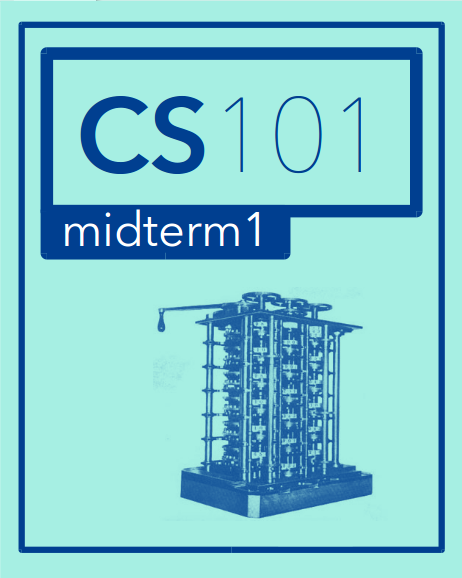
\includegraphics[width=2in]{../img/midterm1-header.png}
\end{center}

\bigskip
\noindent
\begin{itemize}
\item \textbf{Be sure to enter your \underline{NetID} and \underline{the code below} on your Scantron}.
\item Do not turn this page until instructed to do so.
\item There are 30 questions, worth 1 point each.
\item Each question has only \textbf{one} correct answer.
\item You must not communicate with other students during this test.
\item No books, notes, or electronic devices are permitted.
\item This is a 60-minute exam.
\item There are several different versions of this exam.
\end{itemize}

\bigskip\bigskip
\noindent
\textbf{\Large 1. Fill in your information:}

\bigskip
{\Large\bf
\begin{tabular}{ll}
Full Name: & \underbar{\hskip 8cm} \\[0.5em]
UIN (Student Number): & \underbar{\hskip 8cm} \\[0.5em]
NetID: & \underbar{\hskip 8cm}
\end{tabular}
}

\bigskip
\bigskip
\noindent
\textbf{\Large 2. Fill in the following answers on the Scantron form:}

%%%%%%%%%%%%%%%%%%%%%%%%%%%%%%%%%%%%%%%%%%%%%%%%%%%%%%%%%
%%%%%%%%%%%%%%%%%%%%%%%%%%%%%%%%%%%%%%%%%%%%%%%%%%%%%%%%%

\begin{enumerate}
\item[92.] D
\item[93.] E
\item[94.] A
\item[95.] A
\item[96.] D
\end{enumerate}

\newpage

% Zone 1


%%%%%%%%%%%%%%%%%%%%%%%%%%%%%%%%%%%%%%%%%%%%%%%%%%%%%%%%%



\newpage
\noindent
1. (1 point)
Consider the following program:
\begin{verbatim}
s="ECTOR"
t="GAWAIN"
x=(len(s)/(len(t)-1))+1
\end{verbatim}
What is the \textbf{type} of \texttt{x} after this program is executed?


\begin{enumerate}
\item[(A)]
\begin{verbatim}String\end{verbatim}

\item[(B)]
\begin{verbatim}None\end{verbatim}

\item[(C)]
\begin{verbatim}Integer\end{verbatim}

\item[(D)]
\begin{verbatim}Boolean\end{verbatim}

\item[(E)] $\bigstar$ 
\begin{verbatim}Float\end{verbatim}

\end{enumerate}

\vspace*{2em}
\hrule
\vspace{2em}

\noindent {\bf Solution.} 
\vspace{2em}
\hrule height 2pt


\newpage
\noindent
2. (1 point)
Consider the following incomplete function.
\begin{verbatim}
def ismultiple(m,n):
    if ???:
        return False
    else:
        return True
\end{verbatim}
The function is intended to return True if the input parameter m is a multiple of parameter n and False otherwise. For example, \verb|ismultiple(4,2)| should return \verb|True|, but \verb|ismultiple(5,3)| should return \verb|False|. What should replace the three question marks to complete the function?


\begin{enumerate}
\item[(A)] $\bigstar$ 
\begin{verbatim}(m % n) != 0 \end{verbatim}

\item[(B)]
\begin{verbatim}(m // n) != 0 \end{verbatim}

\item[(C)]
\begin{verbatim}(n // m) == 0 \end{verbatim}

\item[(D)]
\begin{verbatim}(n % m) == 0 \end{verbatim}

\end{enumerate}

\vspace*{2em}
\hrule
\vspace{2em}

\noindent {\bf Solution.} 
\vspace{2em}
\hrule height 2pt


\newpage
\noindent
3. (1 point)
For this problem, you should compose a function which accomplishes a given task using the available code blocks arranged in the correct functional order.  \emph{We ignore indentation for this problem.}

\texttt{find\_max} should accept a \texttt{list} and return the value of the maximum item in the \texttt{list}.  (\texttt{None} is always the lowest value in any numeric comparison, so you may use it as an initializer.)

\begin{verbatim}
def find_max(my_list):
\end{verbatim}

\begin{enumerate}[1]
\item \texttt{max\_val = i}
\item \texttt{max\_val = None}
\item \texttt{for i in range(len(my\_list)):}
\item \texttt{if i > max\_val:}
\item \texttt{max\_val = my\_list[i]}
\item \texttt{return max\_val}
\item \texttt{for i in range(my\_list):}
\item \texttt{if my\_list[i] > max\_val:}
\item \texttt{print(max\_val)}
\end{enumerate}



\begin{enumerate}
\item[(A)] $\bigstar$ 
2, 3, 8, 5, 6

\item[(B)]
2, 3, 8, 1, 6

\item[(C)]
3, 2, 8, 5, 9

\item[(D)]
2, 7, 4, 5, 6

\item[(E)]
2, 3, 4, 1, 6

\end{enumerate}

\vspace*{2em}
\hrule
\vspace{2em}

\noindent {\bf Solution.} 
\vspace{2em}
\hrule height 2pt


\newpage
\noindent
4. (1 point)
Consider the following program.
\begin{verbatim}
x=0
i=1
while(i*i)<=9:
    x=x+(i*i)
    i=i+1
\end{verbatim}
After it is run, what is the final \textbf{value} of \texttt{x}?


\begin{enumerate}
\item[(A)]
\begin{verbatim}5\end{verbatim}

\item[(B)] $\bigstar$ 
\begin{verbatim}14\end{verbatim}

\item[(C)]
\begin{verbatim}30\end{verbatim}

\item[(D)]
\begin{verbatim}4\end{verbatim}

\item[(E)]
\begin{verbatim}3\end{verbatim}

\end{enumerate}

\vspace*{2em}
\hrule
\vspace{2em}

\noindent {\bf Solution.} 
\vspace{2em}
\hrule height 2pt


\newpage
\noindent
5. (1 point)
How can the following mathematical equation be implemented as a Python expression? Assume \verb|a|, \verb|b|, and \verb|sin| have already been defined.
$$a \sin(a^b - b)$$


\begin{enumerate}
\item[(A)]
\begin{verbatim}a*sin(b^a - b)\end{verbatim}

\item[(B)]
\begin{verbatim}a*sin(a^b - b)\end{verbatim}

\item[(C)]
\begin{verbatim}a sin(a**b - b)\end{verbatim}

\item[(D)] $\bigstar$ 
\begin{verbatim}a*sin(a**b - b)\end{verbatim}

\item[(E)]
None of the other answers are correct.

\end{enumerate}

\vspace*{2em}
\hrule
\vspace{2em}

\noindent {\bf Solution.} 
\vspace{2em}
\hrule height 2pt


\newpage
\noindent
6. (1 point)
Consider the following program:
\begin{verbatim}
s="TRIS %i"
t="ISEU"
x=s % len(t)
\end{verbatim}
What is the \textbf{type} of \texttt{x} after this program is executed?


\begin{enumerate}
\item[(A)]
\begin{verbatim}None\end{verbatim}

\item[(B)] $\bigstar$ 
\begin{verbatim}String\end{verbatim}

\item[(C)]
\begin{verbatim}Float\end{verbatim}

\item[(D)]
\begin{verbatim}Integer\end{verbatim}

\item[(E)]
\begin{verbatim}Boolean\end{verbatim}

\end{enumerate}

\vspace*{2em}
\hrule
\vspace{2em}

\noindent {\bf Solution.} 
\vspace{2em}
\hrule height 2pt


\newpage
\noindent
7. (1 point)
Consider the following incomplete program.
\begin{verbatim}
sum=0
for i in range(0,100):
    ???

\end{verbatim}
The program is intended to sum all of the integers between 1 and 100 (inclusive). What should replace the three question marks to complete the program?


\begin{enumerate}
\item[(A)] $\bigstar$ 
\begin{verbatim}sum=sum+i+1 \end{verbatim}

\item[(B)]
\begin{verbatim}sum=sum+i \end{verbatim}

\item[(C)]
\begin{verbatim}sum+1=sum \end{verbatim}

\item[(D)]
\begin{verbatim}sum=sum+1\end{verbatim}

\end{enumerate}

\vspace*{2em}
\hrule
\vspace{2em}

\noindent {\bf Solution.} 
\vspace{2em}
\hrule height 2pt


\newpage
\noindent
8. (1 point)
Consider the following program:
\begin{verbatim}
a=3
b=4
if a==3:
    a=b
elif a==4:
    a=5
else:
    b=a
\end{verbatim}
What is the \textbf{value} of a after this program is executed?


\begin{enumerate}
\item[(A)] $\bigstar$ 
\begin{verbatim}4\end{verbatim}

\item[(B)]
\begin{verbatim}7\end{verbatim}

\item[(C)]
None of the other answers are correct.

\item[(D)]
\begin{verbatim}3\end{verbatim}

\item[(E)]
\begin{verbatim}5\end{verbatim}

\end{enumerate}

\vspace*{2em}
\hrule
\vspace{2em}

\noindent {\bf Solution.} 
\vspace{2em}
\hrule height 2pt


\newpage
\noindent
9. (1 point)
Consider the following program:
\begin{verbatim}
def fix(s):
    a=list(s)
    a.sort()
    return ''.join(a)

x=["one","two","eleven","twelve"]
s1=fix(x[0]+x[-1])
s2=fix(x[1]+x[-2])

if s1==s2:
    x.sort()
elif s1<s2:
    x.reverse()
else:
    x.append("six")
\end{verbatim}
What is the \textbf{value} of \texttt{x} after this program is executed?


\begin{enumerate}
\item[(A)] $\bigstar$ 
\begin{verbatim}['eleven', 'one', 'twelve', 'two']\end{verbatim}

\item[(B)]
\begin{verbatim}['one', 'two', 'eleven', 'twelve', 'six']\end{verbatim}

\item[(C)]
\begin{verbatim}['one', 'two', 'eleven', 'twelve']\end{verbatim}

\item[(D)]
\begin{verbatim}['two', 'twelve', 'one', 'eleven', 'six']\end{verbatim}

\item[(E)]
\begin{verbatim}['twelve', 'eleven', 'two', 'one']\end{verbatim}

\end{enumerate}

\vspace*{2em}
\hrule
\vspace{2em}

\noindent {\bf Solution.} 
\vspace{2em}
\hrule height 2pt


\newpage
\noindent
10. (1 point)
What is the result of the following expression?
\begin{verbatim}
[ 1, 2, 3 ] * 3
\end{verbatim}


\begin{enumerate}
\item[(A)] $\bigstar$ 
\begin{verbatim}[1, 2, 3, 1, 2, 3, 1, 2, 3]\end{verbatim}

\item[(B)]
\begin{verbatim}[3, 6, 9]\end{verbatim}

\item[(C)]
\begin{verbatim}[1.0, 2.0, 3.0, 1.0, 2.0, 3.0, 1.0, 2.0, 3.0]\end{verbatim}

\item[(D)]
\begin{verbatim}(3, 6, 9)\end{verbatim}

\item[(E)]
\begin{verbatim}[3.0, 6.0, 9.0]\end{verbatim}

\end{enumerate}

\vspace*{2em}
\hrule
\vspace{2em}

\noindent {\bf Solution.} 
\vspace{2em}
\hrule height 2pt


\newpage
\noindent
11. (1 point)
Consider the following program:
\begin{verbatim}
pi="3.14159"
e="2.71828"
x=(float(e)**float(pi)-float(pi)) == 20
\end{verbatim}
What is the \textbf{type} of \texttt{x} after this program is executed?


\begin{enumerate}
\item[(A)] $\bigstar$ 
\begin{verbatim}Boolean\end{verbatim}

\item[(B)]
\begin{verbatim}Integer\end{verbatim}

\item[(C)]
\begin{verbatim}None\end{verbatim}

\item[(D)]
\begin{verbatim}String\end{verbatim}

\item[(E)]
\begin{verbatim}Float\end{verbatim}

\end{enumerate}

\vspace*{2em}
\hrule
\vspace{2em}

\noindent {\bf Solution.} 
\vspace{2em}
\hrule height 2pt


\newpage
\noindent
12. (1 point)
Consider the following program:
\begin{verbatim}
i=3
x=2
while i < 7:
    x+=i
    i+=2
\end{verbatim}
What is the \textbf{value} of \texttt{x} after this program is executed?


\begin{enumerate}
\item[(A)] $\bigstar$ 
\begin{verbatim}10\end{verbatim}

\item[(B)]
\begin{verbatim}14\end{verbatim}

\item[(C)]
\begin{verbatim}11\end{verbatim}

\item[(D)]
\begin{verbatim}13\end{verbatim}

\item[(E)]
\begin{verbatim}12\end{verbatim}

\end{enumerate}

\vspace*{2em}
\hrule
\vspace{2em}

\noindent {\bf Solution.} 
\vspace{2em}
\hrule height 2pt


\newpage
\noindent
13. (1 point)
Consider the following program:
\begin{verbatim}
x=3
a=5
if (a%3)==2:
    x=x**3
elif(a%3)==1:
    x=x**2
else:
    x=x**1
\end{verbatim}
What is the \textbf{value} of \texttt{x} after this program is executed?


\begin{enumerate}
\item[(A)]
\begin{verbatim}9\end{verbatim}

\item[(B)]
\begin{verbatim}3\end{verbatim}

\item[(C)] $\bigstar$ 
\begin{verbatim}27\end{verbatim}

\item[(D)]
None of the other answers are correct.

\item[(E)]
\begin{verbatim}1\end{verbatim}

\end{enumerate}

\vspace*{2em}
\hrule
\vspace{2em}

\noindent {\bf Solution.} 
\vspace{2em}
\hrule height 2pt


\newpage
\noindent
14. (1 point)
Consider the following program:
\begin{verbatim}
x="KING ARTHUR-MORGANA LEFAY-SIR BEDIVERE".split("-")
y=x
x=y.reverse()
\end{verbatim}
What is the \textbf{value} of \texttt{x} after this program is executed?


\begin{enumerate}
\item[(A)] $\bigstar$ 
\begin{verbatim}None\end{verbatim}

\item[(B)]
\begin{verbatim}['KING', 'ARTHUR-MORGANA', 'LEFAY-SIR', 'BEDIVERE']\end{verbatim}

\item[(C)]
\begin{verbatim}['BEDIVERE', 'LEFAY-SIR', 'ARTHUR-MORGANA', 'KING']\end{verbatim}

\item[(D)]
\begin{verbatim}['SIR BEDIVERE', 'MORGANA LEFAY', 'KING ARTHUR']\end{verbatim}

\item[(E)]
\begin{verbatim}['KING ARTHUR', 'MORGANA LEFAY', 'SIR BEDIVERE']\end{verbatim}

\end{enumerate}

\vspace*{2em}
\hrule
\vspace{2em}

\noindent {\bf Solution.} 
\vspace{2em}
\hrule height 2pt


\newpage
\noindent
15. (1 point)
Consider the following program:
\begin{verbatim}
x=[1,2,3]
def f(a):
    s=""
    a.reverse()
    for i in a:
        s+=str(i)
    return s

x.append(f(x))
\end{verbatim}
What is the \textbf{value} of \texttt{x} after this program is executed?


\begin{enumerate}
\item[(A)]
\begin{verbatim}[1, 2, 3]\end{verbatim}

\item[(B)]
\begin{verbatim}[3, 2, 1]\end{verbatim}

\item[(C)]
\begin{verbatim}[1, 2, 3, '321']\end{verbatim}

\item[(D)]
\begin{verbatim}[1, 2, 3, 6]\end{verbatim}

\item[(E)] $\bigstar$ 
\begin{verbatim}[3, 2, 1, '321']\end{verbatim}

\end{enumerate}

\vspace*{2em}
\hrule
\vspace{2em}

\noindent {\bf Solution.} 
\vspace{2em}
\hrule height 2pt


\newpage
\noindent
16. (1 point)
Consider the following program:
\begin{verbatim}
x=0
for i in range(2,7):
    if i%3==0:
        x+=3
    elif i%2==0:
        x+=2
    else:
        x+=1
\end{verbatim}
What is the \textbf{value} of \texttt{x} after this program is executed?


\begin{enumerate}
\item[(A)]
\begin{verbatim}10\end{verbatim}

\item[(B)]
\begin{verbatim}14\end{verbatim}

\item[(C)]
\begin{verbatim}12\end{verbatim}

\item[(D)]
\begin{verbatim}13\end{verbatim}

\item[(E)] $\bigstar$ 
\begin{verbatim}11\end{verbatim}

\end{enumerate}

\vspace*{2em}
\hrule
\vspace{2em}

\noindent {\bf Solution.} 
\vspace{2em}
\hrule height 2pt


\newpage
\noindent
17. (1 point)
Consider the following program:
\begin{verbatim}
s="G+R+A+I+L"
x=s.split("+")[1:-2]
\end{verbatim}
What is the \textbf{value} of \texttt{x} after this program is executed?


\begin{enumerate}
\item[(A)] $\bigstar$ 
\begin{verbatim}['R','A']\end{verbatim}

\item[(B)]
\begin{verbatim}3\end{verbatim}

\item[(C)]
\begin{verbatim}False\end{verbatim}

\item[(D)]
\begin{verbatim}'RAI'\end{verbatim}

\item[(E)]
\begin{verbatim}None\end{verbatim}

\end{enumerate}

\vspace*{2em}
\hrule
\vspace{2em}

\noindent {\bf Solution.} 
\vspace{2em}
\hrule height 2pt


\newpage
\noindent
18. (1 point)
Consider the following program:
\begin{verbatim}
s="Hobbes"
i=0
x=-1
while i<len(s):
    if s[i]=='b':
        x=i
    i+=1
\end{verbatim}
What is the \textbf{value} of \texttt{x} after this program is executed?


\begin{enumerate}
\item[(A)]
\begin{verbatim}5\end{verbatim}

\item[(B)]
\begin{verbatim}2\end{verbatim}

\item[(C)]
\begin{verbatim}4\end{verbatim}

\item[(D)]
\begin{verbatim}-1\end{verbatim}

\item[(E)] $\bigstar$ 
\begin{verbatim}3\end{verbatim}

\end{enumerate}

\vspace*{2em}
\hrule
\vspace{2em}

\noindent {\bf Solution.} 
\vspace{2em}
\hrule height 2pt


\newpage
\noindent
19. (1 point)
Consider the following program.
\begin{verbatim}
kay = 2
wart = 3

def knight(kay,wart):
    wart += 2
    kay += 3
    return wart + kay

wart = knight(kay, kay) + knight(wart, wart)
\end{verbatim}
After it is run, what is the final \textbf{value} of \texttt{wart}?


\begin{enumerate}
\item[(A)]
\begin{verbatim}5\end{verbatim}

\item[(B)] $\bigstar$ 
None of the other answers are correct.

\item[(C)]
\begin{verbatim}2\end{verbatim}

\item[(D)]
\begin{verbatim}3\end{verbatim}

\end{enumerate}

\vspace*{2em}
\hrule
\vspace{2em}

\noindent {\bf Solution.} 
\vspace{2em}
\hrule height 2pt


\newpage
\noindent
20. (1 point)
Consider the following program:
\begin{verbatim}
a=["merlin","sir agravaine","king pellinore"]
b=[ ]
for i in range(1,3):
    b.append(a[0-i].title())
\end{verbatim}
What is the \textbf{value} of b after this program is executed?


\begin{enumerate}
\item[(A)]
\begin{verbatim}['Merlin', 'King Pellinore', 'Sir Agravaine']\end{verbatim}

\item[(B)]
\begin{verbatim}['Sir Agravaine', 'King Pellinore']\end{verbatim}

\item[(C)]
\begin{verbatim}[ ]\end{verbatim}

\item[(D)]
\begin{verbatim}['King Pellinore', 'Sir Agravaine', 'Merlin']\end{verbatim}

\item[(E)] $\bigstar$ 
\begin{verbatim}['King Pellinore', 'Sir Agravaine']\end{verbatim}

\end{enumerate}

\vspace*{2em}
\hrule
\vspace{2em}

\noindent {\bf Solution.} 
\vspace{2em}
\hrule height 2pt


\newpage
\noindent
21. (1 point)
Consider the following incomplete Python program.
\begin{verbatim}
s="".join(["0","1","2","1"])
x=0
for i in range(len(s)-1):
    x+=int(???)
\end{verbatim}
What should replace the three question marks so the resulting value of \texttt{x} is 34?


\begin{enumerate}
\item[(A)]
\begin{verbatim}s[i:i-1]\end{verbatim}

\item[(B)] $\bigstar$ 
\begin{verbatim}s[i:i+2]\end{verbatim}

\item[(C)]
\begin{verbatim}s[i+1:i+2]\end{verbatim}

\item[(D)]
\begin{verbatim}s[i:i+1]\end{verbatim}

\end{enumerate}

\vspace*{2em}
\hrule
\vspace{2em}

\noindent {\bf Solution.} 
\vspace{2em}
\hrule height 2pt


\newpage
\noindent
22. (1 point)
Consider the following program:
\begin{verbatim}
a=["S","T","U","P","E","F","Y"]
a=a[0:4]
a.sort()
x=""
for e in a:
    x=e+x
\end{verbatim}
What is the \textbf{value} of \texttt{x} after this program is executed?


\begin{enumerate}
\item[(A)] $\bigstar$ 
\begin{verbatim}"UTSP"\end{verbatim}

\item[(B)]
\begin{verbatim}"PSTU"\end{verbatim}

\item[(C)]
\begin{verbatim}"STUP"\end{verbatim}

\item[(D)]
\begin{verbatim}"PUST"\end{verbatim}

\item[(E)]
None of the other answers are correct.

\end{enumerate}

\vspace*{2em}
\hrule
\vspace{2em}

\noindent {\bf Solution.} 
\vspace{2em}
\hrule height 2pt


\newpage
\noindent
23. (1 point)
Consider the following program:
\begin{verbatim}
x=str(1.2)*2
\end{verbatim}
What is the \textbf{value} of \texttt{x} after this program is executed?


\begin{enumerate}
\item[(A)]
\begin{verbatim}"1.2*2"\end{verbatim}

\item[(B)]
None of the other answers are correct.

\item[(C)]
\begin{verbatim}2.4\end{verbatim}

\item[(D)]
\begin{verbatim}"2.4"\end{verbatim}

\item[(E)] $\bigstar$ 
\begin{verbatim}"1.21.2"\end{verbatim}

\end{enumerate}

\vspace*{2em}
\hrule
\vspace{2em}

\noindent {\bf Solution.} 
\vspace{2em}
\hrule height 2pt


\newpage
\noindent
24. (1 point)
Consider the following program:
\begin{verbatim}
x=[1,2,3,4,5,6,7,8,9]
x=x[2:-2]
i=1
while i <= 3:
    x[i]+=1
    i+=1
\end{verbatim}
What is the \textbf{value} of \texttt{x} after this program is executed?


\begin{enumerate}
\item[(A)]
\begin{verbatim}[3, 5, 7, 7]\end{verbatim}

\item[(B)]
\begin{verbatim}[2, 4, 5, 6, 7, 7]\end{verbatim}

\item[(C)]
\begin{verbatim}[3, 5, 6, 7, 7, 8]\end{verbatim}

\item[(D)] $\bigstar$ 
\begin{verbatim}[3, 5, 6, 7, 7]\end{verbatim}

\item[(E)]
\begin{verbatim}[2, 4, 5, 5, 7, 7]\end{verbatim}

\end{enumerate}

\vspace*{2em}
\hrule
\vspace{2em}

\noindent {\bf Solution.} 
\vspace{2em}
\hrule height 2pt


\newpage
\noindent
25. (1 point)
Evaluate the following expression:
\begin{verbatim}
[1,2]*len("3")
\end{verbatim}
What value is produced?


\begin{enumerate}
\item[(A)]
\begin{verbatim}[1,2,1]\end{verbatim}

\item[(B)]
\begin{verbatim}[1,2,1,2,1,2]\end{verbatim}

\item[(C)] $\bigstar$ 
\begin{verbatim}[1,2]\end{verbatim}

\item[(D)]
\begin{verbatim}[1,2,3]\end{verbatim}

\end{enumerate}

\vspace*{2em}
\hrule
\vspace{2em}

\noindent {\bf Solution.} 
\vspace{2em}
\hrule height 2pt


\newpage
\noindent
26. (1 point)
Evaluate the following expression:
\begin{verbatim}
len("ABCDE"[1:4])
\end{verbatim}
What value is produced?


\begin{enumerate}
\item[(A)] $\bigstar$ 
3

\item[(B)]
5

\item[(C)]
1

\item[(D)]
4

\end{enumerate}

\vspace*{2em}
\hrule
\vspace{2em}

\noindent {\bf Solution.} 
\vspace{2em}
\hrule height 2pt


\newpage
\noindent
27. (1 point)
Consider the following Python program.
\begin{verbatim}
e=[1,3,5,7,9,11]
d=[0,0,0]
for i in range(0,len(e)):
    d[i%3]+=e[i]
x=d[2]
\end{verbatim}
After it is run, what is the final \textbf{value} of \texttt{x}?


\begin{enumerate}
\item[(A)]
\begin{verbatim}7\end{verbatim}

\item[(B)] $\bigstar$ 
\begin{verbatim}16\end{verbatim}

\item[(C)]
\begin{verbatim}8\end{verbatim}

\item[(D)]
\begin{verbatim}12\end{verbatim}

\item[(E)]
\begin{verbatim}0\end{verbatim}

\end{enumerate}

\vspace*{2em}
\hrule
\vspace{2em}

\noindent {\bf Solution.} 
\vspace{2em}
\hrule height 2pt


\newpage
\noindent
28. (1 point)
Consider the following program.
\begin{verbatim}
x=[]
for j in range(0,5):
    if (j%4)==0:
        x.append("-")
    if (j%5)==0:
        x.append("*")
\end{verbatim}
After it is run, what is the final \textbf{value} of \texttt{x}?


\begin{enumerate}
\item[(A)]
None of the other answers are correct.

\item[(B)]
\begin{verbatim}["-","*"]\end{verbatim}

\item[(C)] $\bigstar$ 
\begin{verbatim}["-","*","-"]\end{verbatim}

\item[(D)]
\begin{verbatim}["-","-","*"]\end{verbatim}

\item[(E)]
\begin{verbatim}["-","*","*"]\end{verbatim}

\end{enumerate}

\vspace*{2em}
\hrule
\vspace{2em}

\noindent {\bf Solution.} 
\vspace{2em}
\hrule height 2pt


\newpage
\noindent
29. (1 point)
Consider the following program.
\begin{verbatim}
s="BBCAA"
x=0
y=len(s)-1
while s[x]!=s[y] and x<len(s):
    x+=1
    y-=1
\end{verbatim}
After it is run, what is the final \textbf{value} of \texttt{x}?


\begin{enumerate}
\item[(A)] $\bigstar$ 
\begin{verbatim}2\end{verbatim}

\item[(B)]
\begin{verbatim}0\end{verbatim}

\item[(C)]
\begin{verbatim}3\end{verbatim}

\item[(D)]
\begin{verbatim}4\end{verbatim}

\item[(E)]
\begin{verbatim}1\end{verbatim}

\end{enumerate}

\vspace*{2em}
\hrule
\vspace{2em}

\noindent {\bf Solution.} 
\vspace{2em}
\hrule height 2pt


\newpage
\noindent
30. (1 point)
Consider the following program.
\begin{verbatim}
def artificing(s):
    return s+"%i" % 2
    return s*2
    return s

s=artificing("MERLIN")
\end{verbatim}
After it is run, what is the final \textbf{value} of s?


\begin{enumerate}
\item[(A)]
\begin{verbatim}"MERLINMERLIN"\end{verbatim}

\item[(B)]
\begin{verbatim}0\end{verbatim}

\item[(C)] $\bigstar$ 
\begin{verbatim}"MERLIN2"\end{verbatim}

\item[(D)]
\begin{verbatim}None\end{verbatim}

\item[(E)]
\begin{verbatim}"MERLIN%i"\end{verbatim}

\end{enumerate}

\vspace*{2em}
\hrule
\vspace{2em}

\noindent {\bf Solution.} 
\vspace{2em}
\hrule height 2pt

%%%%%%%%%%%%%%%%%%%%%%%%%%%%%%%%%%%%%%%%%%%%%%%%%%%%%%%%%%%%%%%%%%%%%%
%%%%%%%%%%%%%%%%%%%%%%%%%%%%%%%%%%%%%%%%%%%%%%%%%%%%%%%%%%%%%%%%%%%%%%
%%%%%%%%%%%%%%%%%%%%%%%%%%%%%%%%%%%%%%%%%%%%%%%%%%%%%%%%%%%%%%%%%%%%%%
%%%%%%%%%%%%%%%%%%%%%%%%%%%%%%%%%%%%%%%%%%%%%%%%%%%%%%%%%%%%%%%%%%%%%%
% Exam number 25

\message{Exam 25/50}
\cleardoublepage
\setcounter{page}{1}


\begin{center}
%\textbf{\Large CS 101 Midterm \#1}
%
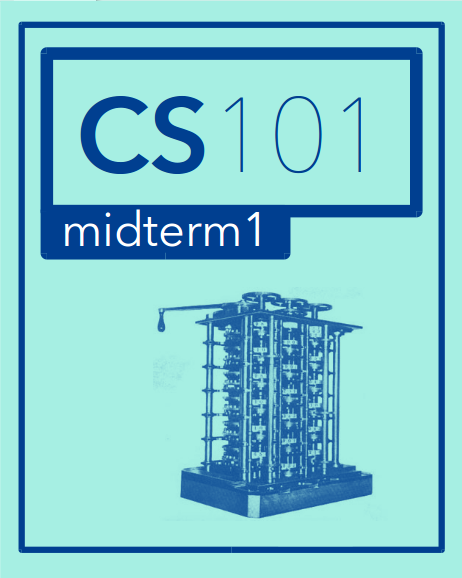
\includegraphics[width=2in]{../img/midterm1-header.png}
\end{center}

\bigskip
\noindent
\begin{itemize}
\item \textbf{Be sure to enter your \underline{NetID} and \underline{the code below} on your Scantron}.
\item Do not turn this page until instructed to do so.
\item There are 30 questions, worth 1 point each.
\item Each question has only \textbf{one} correct answer.
\item You must not communicate with other students during this test.
\item No books, notes, or electronic devices are permitted.
\item This is a 60-minute exam.
\item There are several different versions of this exam.
\end{itemize}

\bigskip\bigskip
\noindent
\textbf{\Large 1. Fill in your information:}

\bigskip
{\Large\bf
\begin{tabular}{ll}
Full Name: & \underbar{\hskip 8cm} \\[0.5em]
UIN (Student Number): & \underbar{\hskip 8cm} \\[0.5em]
NetID: & \underbar{\hskip 8cm}
\end{tabular}
}

\bigskip
\bigskip
\noindent
\textbf{\Large 2. Fill in the following answers on the Scantron form:}

%%%%%%%%%%%%%%%%%%%%%%%%%%%%%%%%%%%%%%%%%%%%%%%%%%%%%%%%%
%%%%%%%%%%%%%%%%%%%%%%%%%%%%%%%%%%%%%%%%%%%%%%%%%%%%%%%%%

\begin{enumerate}
\item[92.] E
\item[93.] E
\item[94.] A
\item[95.] B
\item[96.] E
\end{enumerate}

\newpage

% Zone 1


%%%%%%%%%%%%%%%%%%%%%%%%%%%%%%%%%%%%%%%%%%%%%%%%%%%%%%%%%



\newpage
\noindent
1. (1 point)
Consider the following incomplete Python program.
\begin{verbatim}
s="".join(["1","0","2","1"])
x=0
for i in range(len(s)-1):
    x+=int(???)
\end{verbatim}
What should replace the three question marks so the resulting value of \texttt{x} is 33?


\begin{enumerate}
\item[(A)]
\begin{verbatim}s[i:i-1]\end{verbatim}

\item[(B)]
\begin{verbatim}s[i+1:i+2]\end{verbatim}

\item[(C)] $\bigstar$ 
\begin{verbatim}s[i:i+2]\end{verbatim}

\item[(D)]
\begin{verbatim}s[i:i+1]\end{verbatim}

\end{enumerate}

\vspace*{2em}
\hrule
\vspace{2em}

\noindent {\bf Solution.} 
\vspace{2em}
\hrule height 2pt


\newpage
\noindent
2. (1 point)
Consider the following program:
\begin{verbatim}
s="ECTOR"
t="GAWAIN"
x=len(str(s.isupper()))-t.find("A")
\end{verbatim}
What is the \textbf{type} of \texttt{x} after this program is executed?


\begin{enumerate}
\item[(A)]
\begin{verbatim}Boolean\end{verbatim}

\item[(B)]
\begin{verbatim}None\end{verbatim}

\item[(C)] $\bigstar$ 
\begin{verbatim}Integer\end{verbatim}

\item[(D)]
\begin{verbatim}Float\end{verbatim}

\item[(E)]
\begin{verbatim}String\end{verbatim}

\end{enumerate}

\vspace*{2em}
\hrule
\vspace{2em}

\noindent {\bf Solution.} 
\vspace{2em}
\hrule height 2pt


\newpage
\noindent
3. (1 point)
Consider the following program.
\begin{verbatim}
s="ABCBA"
x=0
y=len(s)-1
while s[x]==s[y] and x<=y:
    x+=1
    y-=1
\end{verbatim}
After it is run, what is the final \textbf{value} of \texttt{x}?


\begin{enumerate}
\item[(A)]
\begin{verbatim}4\end{verbatim}

\item[(B)]
\begin{verbatim}0\end{verbatim}

\item[(C)]
\begin{verbatim}1\end{verbatim}

\item[(D)] $\bigstar$ 
\begin{verbatim}3\end{verbatim}

\item[(E)]
\begin{verbatim}2\end{verbatim}

\end{enumerate}

\vspace*{2em}
\hrule
\vspace{2em}

\noindent {\bf Solution.} 
\vspace{2em}
\hrule height 2pt


\newpage
\noindent
4. (1 point)
Consider the following program.
\begin{verbatim}
x=0
i=1
while(i*i)<=9:
    x=x+(i*i)
    i=i+1
\end{verbatim}
After it is run, what is the final \textbf{value} of \texttt{x}?


\begin{enumerate}
\item[(A)]
\begin{verbatim}5\end{verbatim}

\item[(B)]
\begin{verbatim}30\end{verbatim}

\item[(C)]
\begin{verbatim}4\end{verbatim}

\item[(D)]
\begin{verbatim}3\end{verbatim}

\item[(E)] $\bigstar$ 
\begin{verbatim}14\end{verbatim}

\end{enumerate}

\vspace*{2em}
\hrule
\vspace{2em}

\noindent {\bf Solution.} 
\vspace{2em}
\hrule height 2pt


\newpage
\noindent
5. (1 point)
Consider the following program:
\begin{verbatim}
x="KING ARTHUR-MORGANA LEFAY-SIR BEDIVERE".split("-")
y=x
x=y.reverse()
\end{verbatim}
What is the \textbf{value} of \texttt{x} after this program is executed?


\begin{enumerate}
\item[(A)]
\begin{verbatim}['SIR BEDIVERE', 'MORGANA LEFAY', 'KING ARTHUR']\end{verbatim}

\item[(B)]
\begin{verbatim}['KING ARTHUR', 'MORGANA LEFAY', 'SIR BEDIVERE']\end{verbatim}

\item[(C)]
\begin{verbatim}['KING', 'ARTHUR-MORGANA', 'LEFAY-SIR', 'BEDIVERE']\end{verbatim}

\item[(D)]
\begin{verbatim}['BEDIVERE', 'LEFAY-SIR', 'ARTHUR-MORGANA', 'KING']\end{verbatim}

\item[(E)] $\bigstar$ 
\begin{verbatim}None\end{verbatim}

\end{enumerate}

\vspace*{2em}
\hrule
\vspace{2em}

\noindent {\bf Solution.} 
\vspace{2em}
\hrule height 2pt


\newpage
\noindent
6. (1 point)
Consider the following program:
\begin{verbatim}
s="Hobbes"
i=0
x=-1
while i<len(s):
    if s[i]=='b':
        x=i
    i+=1
\end{verbatim}
What is the \textbf{value} of \texttt{x} after this program is executed?


\begin{enumerate}
\item[(A)]
\begin{verbatim}5\end{verbatim}

\item[(B)]
\begin{verbatim}-1\end{verbatim}

\item[(C)] $\bigstar$ 
\begin{verbatim}3\end{verbatim}

\item[(D)]
\begin{verbatim}4\end{verbatim}

\item[(E)]
\begin{verbatim}2\end{verbatim}

\end{enumerate}

\vspace*{2em}
\hrule
\vspace{2em}

\noindent {\bf Solution.} 
\vspace{2em}
\hrule height 2pt


\newpage
\noindent
7. (1 point)
For this problem, you should compose a function which accomplishes a given task using the available code blocks arranged in the correct functional order.  \emph{We ignore indentation for this problem.}

\texttt{find\_max} should accept a \texttt{list} and return the value of the maximum item in the \texttt{list}.  (\texttt{None} is always the lowest value in any numeric comparison, so you may use it as an initializer.)

\begin{verbatim}
def find_max(my_list):
\end{verbatim}

\begin{enumerate}[1]
\item \texttt{max\_val = i}
\item \texttt{max\_val = None}
\item \texttt{for i in range(len(my\_list)):}
\item \texttt{if i > max\_val:}
\item \texttt{max\_val = my\_list[i]}
\item \texttt{return max\_val}
\item \texttt{for i in range(my\_list):}
\item \texttt{if my\_list[i] > max\_val:}
\item \texttt{print(max\_val)}
\end{enumerate}



\begin{enumerate}
\item[(A)]
2, 3, 8, 1, 6

\item[(B)] $\bigstar$ 
2, 3, 8, 5, 6

\item[(C)]
2, 3, 4, 1, 6

\item[(D)]
2, 7, 4, 5, 6

\item[(E)]
3, 2, 8, 5, 9

\end{enumerate}

\vspace*{2em}
\hrule
\vspace{2em}

\noindent {\bf Solution.} 
\vspace{2em}
\hrule height 2pt


\newpage
\noindent
8. (1 point)
Consider the following program:
\begin{verbatim}
s="G+R+A+I+L"
x=s.split("+")[1:-2]
\end{verbatim}
What is the \textbf{value} of \texttt{x} after this program is executed?


\begin{enumerate}
\item[(A)]
\begin{verbatim}'RAI'\end{verbatim}

\item[(B)]
\begin{verbatim}3\end{verbatim}

\item[(C)]
\begin{verbatim}False\end{verbatim}

\item[(D)] $\bigstar$ 
\begin{verbatim}['R','A']\end{verbatim}

\item[(E)]
\begin{verbatim}None\end{verbatim}

\end{enumerate}

\vspace*{2em}
\hrule
\vspace{2em}

\noindent {\bf Solution.} 
\vspace{2em}
\hrule height 2pt


\newpage
\noindent
9. (1 point)
Consider the following program:
\begin{verbatim}
x=[1,2,3]
def f(a):
    s=""
    a.append(4)
    for i in a:
        s+=str(i)
    return s

x.append(f(x))
\end{verbatim}
What is the \textbf{value} of \texttt{x} after this program is executed?


\begin{enumerate}
\item[(A)]
\begin{verbatim}[1, 2, 3, '123']\end{verbatim}

\item[(B)] $\bigstar$ 
\begin{verbatim}[1, 2, 3, 4, '1234']\end{verbatim}

\item[(C)]
\begin{verbatim}[1, 2, 3, 10]\end{verbatim}

\item[(D)]
\begin{verbatim}[1, 2, 3, '1234']\end{verbatim}

\item[(E)]
\begin{verbatim}[1, 2, 3]\end{verbatim}

\end{enumerate}

\vspace*{2em}
\hrule
\vspace{2em}

\noindent {\bf Solution.} 
\vspace{2em}
\hrule height 2pt


\newpage
\noindent
10. (1 point)
Consider the following program:
\begin{verbatim}
pi="3.14159"
e="2.71828"
x=pi in pi*len(e)
\end{verbatim}
What is the \textbf{type} of \texttt{x} after this program is executed?


\begin{enumerate}
\item[(A)]
\begin{verbatim}Integer\end{verbatim}

\item[(B)]
\begin{verbatim}None\end{verbatim}

\item[(C)] $\bigstar$ 
\begin{verbatim}Boolean\end{verbatim}

\item[(D)]
\begin{verbatim}String\end{verbatim}

\item[(E)]
\begin{verbatim}Float\end{verbatim}

\end{enumerate}

\vspace*{2em}
\hrule
\vspace{2em}

\noindent {\bf Solution.} 
\vspace{2em}
\hrule height 2pt


\newpage
\noindent
11. (1 point)
Consider the following incomplete program.
\begin{verbatim}
sum=0
for i in range(0,100):
    ???

\end{verbatim}
The program is intended to sum all of the integers between 1 and 100 (inclusive). What should replace the three question marks to complete the program?


\begin{enumerate}
\item[(A)]
\begin{verbatim}sum=sum+1\end{verbatim}

\item[(B)]
\begin{verbatim}sum+1=sum \end{verbatim}

\item[(C)] $\bigstar$ 
\begin{verbatim}sum=sum+i+1 \end{verbatim}

\item[(D)]
\begin{verbatim}sum=sum+i \end{verbatim}

\end{enumerate}

\vspace*{2em}
\hrule
\vspace{2em}

\noindent {\bf Solution.} 
\vspace{2em}
\hrule height 2pt


\newpage
\noindent
12. (1 point)
Consider the following program:
\begin{verbatim}
x=3
a=5
if (a%3)==2:
    x=x**3
elif(a%3)==1:
    x=x**2
else:
    x=x**1
\end{verbatim}
What is the \textbf{value} of \texttt{x} after this program is executed?


\begin{enumerate}
\item[(A)] $\bigstar$ 
\begin{verbatim}27\end{verbatim}

\item[(B)]
\begin{verbatim}1\end{verbatim}

\item[(C)]
\begin{verbatim}3\end{verbatim}

\item[(D)]
None of the other answers are correct.

\item[(E)]
\begin{verbatim}9\end{verbatim}

\end{enumerate}

\vspace*{2em}
\hrule
\vspace{2em}

\noindent {\bf Solution.} 
\vspace{2em}
\hrule height 2pt


\newpage
\noindent
13. (1 point)
Consider the following program:
\begin{verbatim}
x=[1,2,3,4,5,6,7,8,9]
x=x[2:-2]
i=1
while i < 3:
    x[i]+=1
    i+=1
\end{verbatim}
What is the \textbf{value} of \texttt{x} after this program is executed?


\begin{enumerate}
\item[(A)] $\bigstar$ 
\begin{verbatim}[3, 5, 6, 6, 7]\end{verbatim}

\item[(B)]
\begin{verbatim}[2, 4, 5, 5, 6, 7]\end{verbatim}

\item[(C)]
\begin{verbatim}[3, 5, 6, 6]\end{verbatim}

\item[(D)]
\begin{verbatim}[3, 5, 6, 6, 7, 8]\end{verbatim}

\item[(E)]
\begin{verbatim}[2, 4, 5, 6, 6, 7]\end{verbatim}

\end{enumerate}

\vspace*{2em}
\hrule
\vspace{2em}

\noindent {\bf Solution.} 
\vspace{2em}
\hrule height 2pt


\newpage
\noindent
14. (1 point)
Consider the following program:
\begin{verbatim}
def fix(s):
    a=list(s)
    a.sort()
    return ''.join(a)

x=["one","two","eleven","twelve"]
s1=fix(x[0]+x[-1])
s2=fix(x[1]+x[-2])

if s1<s2:
    x.sort()
elif s1>s2:
    x.reverse()
else:
    x.append("six")
\end{verbatim}
What is the \textbf{value} of \texttt{x} after this program is executed?


\begin{enumerate}
\item[(A)]
\begin{verbatim}['one', 'two', 'eleven', 'twelve']\end{verbatim}

\item[(B)]
\begin{verbatim}['eleven', 'one', 'twelve', 'two']\end{verbatim}

\item[(C)] $\bigstar$ 
\begin{verbatim}['one', 'two', 'eleven', 'twelve', 'six']\end{verbatim}

\item[(D)]
\begin{verbatim}['two', 'twelve', 'one', 'eleven', 'six']\end{verbatim}

\item[(E)]
\begin{verbatim}['twelve', 'eleven', 'two', 'one']\end{verbatim}

\end{enumerate}

\vspace*{2em}
\hrule
\vspace{2em}

\noindent {\bf Solution.} 
\vspace{2em}
\hrule height 2pt


\newpage
\noindent
15. (1 point)
Consider the following incomplete function.
\begin{verbatim}
def ismultiple(m,n):
    if ???:
        return False
    else:
        return True
\end{verbatim}
The function is intended to return True if the input parameter m is a multiple of parameter n and False otherwise. For example, \verb|ismultiple(4,2)| should return \verb|True|, but \verb|ismultiple(5,3)| should return \verb|False|. What should replace the three question marks to complete the function?


\begin{enumerate}
\item[(A)]
\begin{verbatim}(n % m) == 0 \end{verbatim}

\item[(B)]
\begin{verbatim}(m // n) != 0 \end{verbatim}

\item[(C)] $\bigstar$ 
\begin{verbatim}(m % n) != 0 \end{verbatim}

\item[(D)]
\begin{verbatim}(n // m) == 0 \end{verbatim}

\end{enumerate}

\vspace*{2em}
\hrule
\vspace{2em}

\noindent {\bf Solution.} 
\vspace{2em}
\hrule height 2pt


\newpage
\noindent
16. (1 point)
Evaluate the following expression:
\begin{verbatim}
len("ABCD"[0:3])
\end{verbatim}
What value is produced?


\begin{enumerate}
\item[(A)]
4

\item[(B)]
2

\item[(C)]
1

\item[(D)] $\bigstar$ 
3

\end{enumerate}

\vspace*{2em}
\hrule
\vspace{2em}

\noindent {\bf Solution.} 
\vspace{2em}
\hrule height 2pt


\newpage
\noindent
17. (1 point)
Evaluate the following expression:
\begin{verbatim}
[1,2]*len("3")
\end{verbatim}
What value is produced?


\begin{enumerate}
\item[(A)] $\bigstar$ 
\begin{verbatim}[1,2]\end{verbatim}

\item[(B)]
\begin{verbatim}[1,2,1,2,1,2]\end{verbatim}

\item[(C)]
\begin{verbatim}[1,2,3]\end{verbatim}

\item[(D)]
\begin{verbatim}[1,2,1]\end{verbatim}

\end{enumerate}

\vspace*{2em}
\hrule
\vspace{2em}

\noindent {\bf Solution.} 
\vspace{2em}
\hrule height 2pt


\newpage
\noindent
18. (1 point)
Consider the following program:
\begin{verbatim}
i=3
x=2
while i < 7:
    x+=i
    i+=2
\end{verbatim}
What is the \textbf{value} of \texttt{x} after this program is executed?


\begin{enumerate}
\item[(A)] $\bigstar$ 
\begin{verbatim}10\end{verbatim}

\item[(B)]
\begin{verbatim}11\end{verbatim}

\item[(C)]
\begin{verbatim}14\end{verbatim}

\item[(D)]
\begin{verbatim}12\end{verbatim}

\item[(E)]
\begin{verbatim}13\end{verbatim}

\end{enumerate}

\vspace*{2em}
\hrule
\vspace{2em}

\noindent {\bf Solution.} 
\vspace{2em}
\hrule height 2pt


\newpage
\noindent
19. (1 point)
Consider the following program:
\begin{verbatim}
s="TRIS %i"
t="ISEU"
x=s % len(t)
\end{verbatim}
What is the \textbf{type} of \texttt{x} after this program is executed?


\begin{enumerate}
\item[(A)]
\begin{verbatim}Boolean\end{verbatim}

\item[(B)]
\begin{verbatim}Float\end{verbatim}

\item[(C)] $\bigstar$ 
\begin{verbatim}String\end{verbatim}

\item[(D)]
\begin{verbatim}None\end{verbatim}

\item[(E)]
\begin{verbatim}Integer\end{verbatim}

\end{enumerate}

\vspace*{2em}
\hrule
\vspace{2em}

\noindent {\bf Solution.} 
\vspace{2em}
\hrule height 2pt


\newpage
\noindent
20. (1 point)
Consider the following program.
\begin{verbatim}
kay = 2
wart = 3

def knight(kay,wart):
    wart += 2
    kay += 3
    return wart + kay

kay = knight(wart, kay) + knight(kay, wart)
\end{verbatim}
After it is run, what is the final \textbf{value} of \texttt{kay}?


\begin{enumerate}
\item[(A)] $\bigstar$ 
None of the other answers are correct.

\item[(B)]
\begin{verbatim}3\end{verbatim}

\item[(C)]
\begin{verbatim}5\end{verbatim}

\item[(D)]
\begin{verbatim}2\end{verbatim}

\end{enumerate}

\vspace*{2em}
\hrule
\vspace{2em}

\noindent {\bf Solution.} 
\vspace{2em}
\hrule height 2pt


\newpage
\noindent
21. (1 point)
Consider the following program:
\begin{verbatim}
a=["merlin","sir agravaine","king pellinore"]
b=[ ]
for i in range(1,3):
    b.append(a[0-i].title())
\end{verbatim}
What is the \textbf{value} of b after this program is executed?


\begin{enumerate}
\item[(A)]
\begin{verbatim}['Merlin', 'King Pellinore', 'Sir Agravaine']\end{verbatim}

\item[(B)]
\begin{verbatim}['Sir Agravaine', 'King Pellinore']\end{verbatim}

\item[(C)] $\bigstar$ 
\begin{verbatim}['King Pellinore', 'Sir Agravaine']\end{verbatim}

\item[(D)]
\begin{verbatim}[ ]\end{verbatim}

\item[(E)]
\begin{verbatim}['King Pellinore', 'Sir Agravaine', 'Merlin']\end{verbatim}

\end{enumerate}

\vspace*{2em}
\hrule
\vspace{2em}

\noindent {\bf Solution.} 
\vspace{2em}
\hrule height 2pt


\newpage
\noindent
22. (1 point)
Consider the following program.
\begin{verbatim}
x=[]
for j in range(0,5):
    if (j%4)==0:
        x.append("-")
    if (j%5)==0:
        x.append("*")
\end{verbatim}
After it is run, what is the final \textbf{value} of \texttt{x}?


\begin{enumerate}
\item[(A)] $\bigstar$ 
\begin{verbatim}["-","*","-"]\end{verbatim}

\item[(B)]
\begin{verbatim}["-","*","*"]\end{verbatim}

\item[(C)]
None of the other answers are correct.

\item[(D)]
\begin{verbatim}["-","-","*"]\end{verbatim}

\item[(E)]
\begin{verbatim}["-","*"]\end{verbatim}

\end{enumerate}

\vspace*{2em}
\hrule
\vspace{2em}

\noindent {\bf Solution.} 
\vspace{2em}
\hrule height 2pt


\newpage
\noindent
23. (1 point)
Consider the following program:
\begin{verbatim}
a=3
b=4
if a!=b:
    a=b
elif a==4:
    a=5
else:
    b=a
\end{verbatim}
What is the \textbf{value} of a after this program is executed?


\begin{enumerate}
\item[(A)] $\bigstar$ 
\begin{verbatim}4\end{verbatim}

\item[(B)]
\begin{verbatim}3\end{verbatim}

\item[(C)]
\begin{verbatim}7\end{verbatim}

\item[(D)]
\begin{verbatim}5\end{verbatim}

\item[(E)]
None of the other answers are correct.

\end{enumerate}

\vspace*{2em}
\hrule
\vspace{2em}

\noindent {\bf Solution.} 
\vspace{2em}
\hrule height 2pt


\newpage
\noindent
24. (1 point)
Consider the following program.
\begin{verbatim}
def artificing(s):
    return s+"%i" % 2
    return s*2
    return s

s=artificing("MERLIN")
\end{verbatim}
After it is run, what is the final \textbf{value} of s?


\begin{enumerate}
\item[(A)]
\begin{verbatim}0\end{verbatim}

\item[(B)] $\bigstar$ 
\begin{verbatim}"MERLIN2"\end{verbatim}

\item[(C)]
\begin{verbatim}"MERLINMERLIN"\end{verbatim}

\item[(D)]
\begin{verbatim}None\end{verbatim}

\item[(E)]
\begin{verbatim}"MERLIN%i"\end{verbatim}

\end{enumerate}

\vspace*{2em}
\hrule
\vspace{2em}

\noindent {\bf Solution.} 
\vspace{2em}
\hrule height 2pt


\newpage
\noindent
25. (1 point)
How can the following mathematical equation be implemented as a Python expression? Assume \verb|a|, \verb|b|, and \verb|cos| have already been defined.
$$a^b \cos(a - b)$$


\begin{enumerate}
\item[(A)]
\begin{verbatim}(a**b)cos(a-b)\end{verbatim}

\item[(B)] $\bigstar$ 
\begin{verbatim}(a**b)*cos(a-b)\end{verbatim}

\item[(C)]
None of the other answers are correct.

\item[(D)]
\begin{verbatim}(b^a)cos(a-b)\end{verbatim}

\item[(E)]
\begin{verbatim}(a^b)*cos(a-b)\end{verbatim}

\end{enumerate}

\vspace*{2em}
\hrule
\vspace{2em}

\noindent {\bf Solution.} 
\vspace{2em}
\hrule height 2pt


\newpage
\noindent
26. (1 point)
Consider the following program:
\begin{verbatim}
a=["A","C","C","I","O"]
a.sort()
a[0]=a[-1]
x=""
for e in a:
    x=x+e
\end{verbatim}
What is the \textbf{value} of \texttt{x} after this program is executed?


\begin{enumerate}
\item[(A)]
\begin{verbatim}"ACCOA"\end{verbatim}

\item[(B)]
None of the other answers are correct.

\item[(C)] $\bigstar$ 
\begin{verbatim}"OCCIO"\end{verbatim}

\item[(D)]
\begin{verbatim}"ICCOI"\end{verbatim}

\item[(E)]
\begin{verbatim}"ACCIA"\end{verbatim}

\end{enumerate}

\vspace*{2em}
\hrule
\vspace{2em}

\noindent {\bf Solution.} 
\vspace{2em}
\hrule height 2pt


\newpage
\noindent
27. (1 point)
Consider the following program:
\begin{verbatim}
x=0
for i in range(4,10):
    if i%3==0:
        x+=3
    elif i%2==0:
        x+=2
    else:
        x+=1
\end{verbatim}
What is the \textbf{value} of \texttt{x} after this program is executed?


\begin{enumerate}
\item[(A)]
\begin{verbatim}10\end{verbatim}

\item[(B)]
\begin{verbatim}13\end{verbatim}

\item[(C)]
\begin{verbatim}11\end{verbatim}

\item[(D)] $\bigstar$ 
\begin{verbatim}12\end{verbatim}

\item[(E)]
\begin{verbatim}14\end{verbatim}

\end{enumerate}

\vspace*{2em}
\hrule
\vspace{2em}

\noindent {\bf Solution.} 
\vspace{2em}
\hrule height 2pt


\newpage
\noindent
28. (1 point)
Consider the following Python program.
\begin{verbatim}
e=[1,3,5,7,9,11]
d=[0,0,0]
for i in range(0,len(e)):
    d[i%3]+=e[i]
x=d[2]
\end{verbatim}
After it is run, what is the final \textbf{value} of \texttt{x}?


\begin{enumerate}
\item[(A)]
\begin{verbatim}7\end{verbatim}

\item[(B)]
\begin{verbatim}0\end{verbatim}

\item[(C)]
\begin{verbatim}8\end{verbatim}

\item[(D)] $\bigstar$ 
\begin{verbatim}16\end{verbatim}

\item[(E)]
\begin{verbatim}12\end{verbatim}

\end{enumerate}

\vspace*{2em}
\hrule
\vspace{2em}

\noindent {\bf Solution.} 
\vspace{2em}
\hrule height 2pt


\newpage
\noindent
29. (1 point)
Consider the following program:
\begin{verbatim}
x=str(1.2)*2
\end{verbatim}
What is the \textbf{value} of \texttt{x} after this program is executed?


\begin{enumerate}
\item[(A)]
None of the other answers are correct.

\item[(B)]
\begin{verbatim}"1.2*2"\end{verbatim}

\item[(C)]
\begin{verbatim}"2.4"\end{verbatim}

\item[(D)]
\begin{verbatim}2.4\end{verbatim}

\item[(E)] $\bigstar$ 
\begin{verbatim}"1.21.2"\end{verbatim}

\end{enumerate}

\vspace*{2em}
\hrule
\vspace{2em}

\noindent {\bf Solution.} 
\vspace{2em}
\hrule height 2pt


\newpage
\noindent
30. (1 point)
What is the result of the following expression?
\begin{verbatim}
[ 1, 2, 3 ] * 3
\end{verbatim}


\begin{enumerate}
\item[(A)]
\begin{verbatim}(3, 6, 9)\end{verbatim}

\item[(B)]
\begin{verbatim}[3.0, 6.0, 9.0]\end{verbatim}

\item[(C)]
\begin{verbatim}[1.0, 2.0, 3.0, 1.0, 2.0, 3.0, 1.0, 2.0, 3.0]\end{verbatim}

\item[(D)]
\begin{verbatim}[3, 6, 9]\end{verbatim}

\item[(E)] $\bigstar$ 
\begin{verbatim}[1, 2, 3, 1, 2, 3, 1, 2, 3]\end{verbatim}

\end{enumerate}

\vspace*{2em}
\hrule
\vspace{2em}

\noindent {\bf Solution.} 
\vspace{2em}
\hrule height 2pt

%%%%%%%%%%%%%%%%%%%%%%%%%%%%%%%%%%%%%%%%%%%%%%%%%%%%%%%%%%%%%%%%%%%%%%
%%%%%%%%%%%%%%%%%%%%%%%%%%%%%%%%%%%%%%%%%%%%%%%%%%%%%%%%%%%%%%%%%%%%%%
%%%%%%%%%%%%%%%%%%%%%%%%%%%%%%%%%%%%%%%%%%%%%%%%%%%%%%%%%%%%%%%%%%%%%%
%%%%%%%%%%%%%%%%%%%%%%%%%%%%%%%%%%%%%%%%%%%%%%%%%%%%%%%%%%%%%%%%%%%%%%
% Exam number 26

\message{Exam 26/50}
\cleardoublepage
\setcounter{page}{1}


\begin{center}
%\textbf{\Large CS 101 Midterm \#1}
%
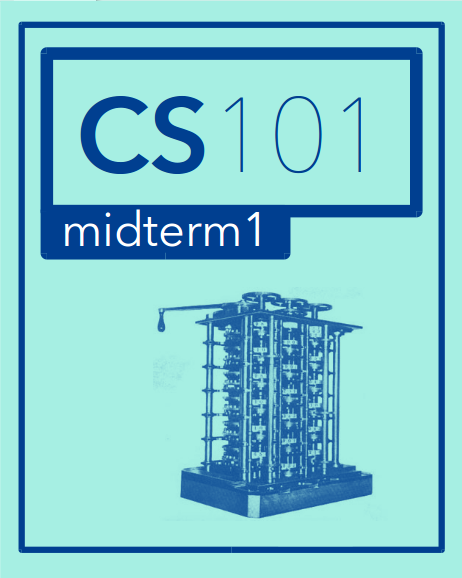
\includegraphics[width=2in]{../img/midterm1-header.png}
\end{center}

\bigskip
\noindent
\begin{itemize}
\item \textbf{Be sure to enter your \underline{NetID} and \underline{the code below} on your Scantron}.
\item Do not turn this page until instructed to do so.
\item There are 30 questions, worth 1 point each.
\item Each question has only \textbf{one} correct answer.
\item You must not communicate with other students during this test.
\item No books, notes, or electronic devices are permitted.
\item This is a 60-minute exam.
\item There are several different versions of this exam.
\end{itemize}

\bigskip\bigskip
\noindent
\textbf{\Large 1. Fill in your information:}

\bigskip
{\Large\bf
\begin{tabular}{ll}
Full Name: & \underbar{\hskip 8cm} \\[0.5em]
UIN (Student Number): & \underbar{\hskip 8cm} \\[0.5em]
NetID: & \underbar{\hskip 8cm}
\end{tabular}
}

\bigskip
\bigskip
\noindent
\textbf{\Large 2. Fill in the following answers on the Scantron form:}

%%%%%%%%%%%%%%%%%%%%%%%%%%%%%%%%%%%%%%%%%%%%%%%%%%%%%%%%%
%%%%%%%%%%%%%%%%%%%%%%%%%%%%%%%%%%%%%%%%%%%%%%%%%%%%%%%%%

\begin{enumerate}
\item[92.] A
\item[93.] A
\item[94.] B
\item[95.] E
\item[96.] A
\end{enumerate}

\newpage

% Zone 1


%%%%%%%%%%%%%%%%%%%%%%%%%%%%%%%%%%%%%%%%%%%%%%%%%%%%%%%%%



\newpage
\noindent
1. (1 point)
Consider the following Python program.
\begin{verbatim}
e=[1,3,5,7,9,11]
d=[0,0,0]
for i in range(0,len(e)):
    d[i%3]+=e[i]
x=d[1]
\end{verbatim}
After it is run, what is the final \textbf{value} of \texttt{x}?


\begin{enumerate}
\item[(A)]
\begin{verbatim}8\end{verbatim}

\item[(B)]
\begin{verbatim}0\end{verbatim}

\item[(C)] $\bigstar$ 
\begin{verbatim}12\end{verbatim}

\item[(D)]
\begin{verbatim}3\end{verbatim}

\item[(E)]
\begin{verbatim}16\end{verbatim}

\end{enumerate}

\vspace*{2em}
\hrule
\vspace{2em}

\noindent {\bf Solution.} 
\vspace{2em}
\hrule height 2pt


\newpage
\noindent
2. (1 point)
Consider the following program:
\begin{verbatim}
x=3
a=7
if (a%3)==2:
    x=x**2
elif(a%3)==1:
    x=x**1
else:
    x=x**0
\end{verbatim}
What is the \textbf{value} of \texttt{x} after this program is executed?


\begin{enumerate}
\item[(A)]
\begin{verbatim}7\end{verbatim}

\item[(B)] $\bigstar$ 
\begin{verbatim}3\end{verbatim}

\item[(C)]
\begin{verbatim}1\end{verbatim}

\item[(D)]
None of the other answers are correct.

\item[(E)]
\begin{verbatim}9\end{verbatim}

\end{enumerate}

\vspace*{2em}
\hrule
\vspace{2em}

\noindent {\bf Solution.} 
\vspace{2em}
\hrule height 2pt


\newpage
\noindent
3. (1 point)
Consider the following program:
\begin{verbatim}
pi="3.14159"
e="2.71828"
x=(float(e)**float(pi)-float(pi)) == 20
\end{verbatim}
What is the \textbf{type} of \texttt{x} after this program is executed?


\begin{enumerate}
\item[(A)]
\begin{verbatim}Float\end{verbatim}

\item[(B)] $\bigstar$ 
\begin{verbatim}Boolean\end{verbatim}

\item[(C)]
\begin{verbatim}Integer\end{verbatim}

\item[(D)]
\begin{verbatim}None\end{verbatim}

\item[(E)]
\begin{verbatim}String\end{verbatim}

\end{enumerate}

\vspace*{2em}
\hrule
\vspace{2em}

\noindent {\bf Solution.} 
\vspace{2em}
\hrule height 2pt


\newpage
\noindent
4. (1 point)
Consider the following program:
\begin{verbatim}
a=3
b=4
if a!=b:
    a=b
elif a==4:
    a=5
else:
    b=a
\end{verbatim}
What is the \textbf{value} of a after this program is executed?


\begin{enumerate}
\item[(A)]
\begin{verbatim}3\end{verbatim}

\item[(B)] $\bigstar$ 
\begin{verbatim}4\end{verbatim}

\item[(C)]
\begin{verbatim}5\end{verbatim}

\item[(D)]
None of the other answers are correct.

\item[(E)]
\begin{verbatim}7\end{verbatim}

\end{enumerate}

\vspace*{2em}
\hrule
\vspace{2em}

\noindent {\bf Solution.} 
\vspace{2em}
\hrule height 2pt


\newpage
\noindent
5. (1 point)
Consider the following program:
\begin{verbatim}
i=2
x=3
while i < 7:
    x+=i
    i+=2
\end{verbatim}
What is the \textbf{value} of \texttt{x} after this program is executed?


\begin{enumerate}
\item[(A)] $\bigstar$ 
\begin{verbatim}15\end{verbatim}

\item[(B)]
\begin{verbatim}14\end{verbatim}

\item[(C)]
\begin{verbatim}12\end{verbatim}

\item[(D)]
\begin{verbatim}11\end{verbatim}

\item[(E)]
\begin{verbatim}13\end{verbatim}

\end{enumerate}

\vspace*{2em}
\hrule
\vspace{2em}

\noindent {\bf Solution.} 
\vspace{2em}
\hrule height 2pt


\newpage
\noindent
6. (1 point)
Consider the following program:
\begin{verbatim}
x=[1,2,3]
def f(a):
    s=""
    a.reverse()
    for i in a:
        s+=str(i)
    return s

x.append(f(x))
\end{verbatim}
What is the \textbf{value} of \texttt{x} after this program is executed?


\begin{enumerate}
\item[(A)]
\begin{verbatim}[3, 2, 1]\end{verbatim}

\item[(B)]
\begin{verbatim}[1, 2, 3, 6]\end{verbatim}

\item[(C)]
\begin{verbatim}[1, 2, 3, '321']\end{verbatim}

\item[(D)] $\bigstar$ 
\begin{verbatim}[3, 2, 1, '321']\end{verbatim}

\item[(E)]
\begin{verbatim}[1, 2, 3]\end{verbatim}

\end{enumerate}

\vspace*{2em}
\hrule
\vspace{2em}

\noindent {\bf Solution.} 
\vspace{2em}
\hrule height 2pt


\newpage
\noindent
7. (1 point)
Consider the following program.
\begin{verbatim}
x=[]
for j in range(0,5):
    if (j%3)==0:
        x.append("-")
    if (j%4)==0:
        x.append("*")
\end{verbatim}
After it is run, what is the final \textbf{value} of \texttt{x}?


\begin{enumerate}
\item[(A)] $\bigstar$ 
\begin{verbatim}["-","*","-","*"]\end{verbatim}

\item[(B)]
\begin{verbatim}["*","-","*"]\end{verbatim}

\item[(C)]
\begin{verbatim}["-","*"]\end{verbatim}

\item[(D)]
None of the other answers are correct.

\item[(E)]
\begin{verbatim}["*","-","*"]\end{verbatim}

\end{enumerate}

\vspace*{2em}
\hrule
\vspace{2em}

\noindent {\bf Solution.} 
\vspace{2em}
\hrule height 2pt


\newpage
\noindent
8. (1 point)
Consider the following program:
\begin{verbatim}
s="ECTOR"
t="GAWAIN"
x=(len(s)+len(t)) < 4 and s in t
\end{verbatim}
What is the \textbf{type} of \texttt{x} after this program is executed?


\begin{enumerate}
\item[(A)]
\begin{verbatim}Float\end{verbatim}

\item[(B)] $\bigstar$ 
\begin{verbatim}Boolean\end{verbatim}

\item[(C)]
\begin{verbatim}Integer\end{verbatim}

\item[(D)]
\begin{verbatim}String\end{verbatim}

\item[(E)]
\begin{verbatim}None\end{verbatim}

\end{enumerate}

\vspace*{2em}
\hrule
\vspace{2em}

\noindent {\bf Solution.} 
\vspace{2em}
\hrule height 2pt


\newpage
\noindent
9. (1 point)
Consider the following program:
\begin{verbatim}
s="TRIS %i"
t="ISEU"
x=len(s) % len(t[2:-1])
\end{verbatim}
What is the \textbf{type} of \texttt{x} after this program is executed?


\begin{enumerate}
\item[(A)]
\begin{verbatim}None\end{verbatim}

\item[(B)]
\begin{verbatim}Boolean\end{verbatim}

\item[(C)]
\begin{verbatim}String\end{verbatim}

\item[(D)] $\bigstar$ 
\begin{verbatim}Integer\end{verbatim}

\item[(E)]
\begin{verbatim}Float\end{verbatim}

\end{enumerate}

\vspace*{2em}
\hrule
\vspace{2em}

\noindent {\bf Solution.} 
\vspace{2em}
\hrule height 2pt


\newpage
\noindent
10. (1 point)
Consider the following incomplete program.
\begin{verbatim}
sum=0
???:
    sum=sum+i

\end{verbatim}
The program is intended to sum all of the integers between 1 and 100 (inclusive). What should replace the three question marks to complete the program?


\begin{enumerate}
\item[(A)] $\bigstar$ 
\begin{verbatim}for i in range(1,101) \end{verbatim}

\item[(B)]
\begin{verbatim}while i in range(100)\end{verbatim}

\item[(C)]
\begin{verbatim}while i<=100 \end{verbatim}

\item[(D)]
\begin{verbatim}for i in range(0,100)\end{verbatim}

\end{enumerate}

\vspace*{2em}
\hrule
\vspace{2em}

\noindent {\bf Solution.} 
\vspace{2em}
\hrule height 2pt


\newpage
\noindent
11. (1 point)
Consider the following program:
\begin{verbatim}
a=["A","C","C","I","O"]
a.sort()
a[0]=a[-1]
x=""
for e in a:
    x=x+e
\end{verbatim}
What is the \textbf{value} of \texttt{x} after this program is executed?


\begin{enumerate}
\item[(A)]
None of the other answers are correct.

\item[(B)]
\begin{verbatim}"ACCOA"\end{verbatim}

\item[(C)] $\bigstar$ 
\begin{verbatim}"OCCIO"\end{verbatim}

\item[(D)]
\begin{verbatim}"ACCIA"\end{verbatim}

\item[(E)]
\begin{verbatim}"ICCOI"\end{verbatim}

\end{enumerate}

\vspace*{2em}
\hrule
\vspace{2em}

\noindent {\bf Solution.} 
\vspace{2em}
\hrule height 2pt


\newpage
\noindent
12. (1 point)
Consider the following program.
\begin{verbatim}
kay = 2
wart = 3

def knight(kay,wart):
    wart += 2
    kay += 3
    return wart + kay

wart = knight(kay, kay) + knight(wart, wart)
\end{verbatim}
After it is run, what is the final \textbf{value} of \texttt{wart}?


\begin{enumerate}
\item[(A)]
\begin{verbatim}2\end{verbatim}

\item[(B)] $\bigstar$ 
None of the other answers are correct.

\item[(C)]
\begin{verbatim}3\end{verbatim}

\item[(D)]
\begin{verbatim}5\end{verbatim}

\end{enumerate}

\vspace*{2em}
\hrule
\vspace{2em}

\noindent {\bf Solution.} 
\vspace{2em}
\hrule height 2pt


\newpage
\noindent
13. (1 point)
Consider the following incomplete Python program.
\begin{verbatim}
s="".join(["1","0","2","1"])
x=0
for i in range(len(s)-1):
    x+=int(???)
\end{verbatim}
What should replace the three question marks so the resulting value of \texttt{x} is 33?


\begin{enumerate}
\item[(A)]
\begin{verbatim}s[i:i+1]\end{verbatim}

\item[(B)]
\begin{verbatim}s[i+1:i+2]\end{verbatim}

\item[(C)]
\begin{verbatim}s[i:i-1]\end{verbatim}

\item[(D)] $\bigstar$ 
\begin{verbatim}s[i:i+2]\end{verbatim}

\end{enumerate}

\vspace*{2em}
\hrule
\vspace{2em}

\noindent {\bf Solution.} 
\vspace{2em}
\hrule height 2pt


\newpage
\noindent
14. (1 point)
Consider the following program:
\begin{verbatim}
a=["merlin","sir agravaine","king pellinore"]
b=[ ]
for i in range(0,3):
    b.append(a[0-i].title())
\end{verbatim}
What is the \textbf{value} of b after this program is executed?


\begin{enumerate}
\item[(A)]
\begin{verbatim}['King Pellinore', 'Sir Agravaine', 'Merlin']\end{verbatim}

\item[(B)]
\begin{verbatim}['Sir Agravaine', 'King Pellinore']\end{verbatim}

\item[(C)]
\begin{verbatim}[ ]\end{verbatim}

\item[(D)] $\bigstar$ 
\begin{verbatim}['Merlin', 'King Pellinore', 'Sir Agravaine']\end{verbatim}

\item[(E)]
\begin{verbatim}['King Pellinore', 'Sir Agravaine']\end{verbatim}

\end{enumerate}

\vspace*{2em}
\hrule
\vspace{2em}

\noindent {\bf Solution.} 
\vspace{2em}
\hrule height 2pt


\newpage
\noindent
15. (1 point)
Consider the following incomplete function.
\begin{verbatim}
def ismultiple(m,n):
    if ???:
        return False
    else:
        return True
\end{verbatim}
The function is intended to return True if the input parameter m is a multiple of parameter n and False otherwise. For example, \verb|ismultiple(4,2)| should return \verb|True|, but \verb|ismultiple(5,3)| should return \verb|False|. What should replace the three question marks to complete the function?


\begin{enumerate}
\item[(A)]
\begin{verbatim}(m // n) != 0 \end{verbatim}

\item[(B)] $\bigstar$ 
\begin{verbatim}(m % n) != 0 \end{verbatim}

\item[(C)]
\begin{verbatim}(n % m) == 0 \end{verbatim}

\item[(D)]
\begin{verbatim}(n // m) == 0 \end{verbatim}

\end{enumerate}

\vspace*{2em}
\hrule
\vspace{2em}

\noindent {\bf Solution.} 
\vspace{2em}
\hrule height 2pt


\newpage
\noindent
16. (1 point)
Consider the following program.
\begin{verbatim}
x=0
i=1
while(i*i)<=9:
    x=x+(i*i)
    i=i+1
\end{verbatim}
After it is run, what is the final \textbf{value} of \texttt{x}?


\begin{enumerate}
\item[(A)]
\begin{verbatim}30\end{verbatim}

\item[(B)]
\begin{verbatim}4\end{verbatim}

\item[(C)] $\bigstar$ 
\begin{verbatim}14\end{verbatim}

\item[(D)]
\begin{verbatim}3\end{verbatim}

\item[(E)]
\begin{verbatim}5\end{verbatim}

\end{enumerate}

\vspace*{2em}
\hrule
\vspace{2em}

\noindent {\bf Solution.} 
\vspace{2em}
\hrule height 2pt


\newpage
\noindent
17. (1 point)
Evaluate the following expression:
\begin{verbatim}
len("ABCD"[0:3])
\end{verbatim}
What value is produced?


\begin{enumerate}
\item[(A)] $\bigstar$ 
3

\item[(B)]
1

\item[(C)]
4

\item[(D)]
2

\end{enumerate}

\vspace*{2em}
\hrule
\vspace{2em}

\noindent {\bf Solution.} 
\vspace{2em}
\hrule height 2pt


\newpage
\noindent
18. (1 point)
Evaluate the following expression:
\begin{verbatim}
[1,2]*len("3")
\end{verbatim}
What value is produced?


\begin{enumerate}
\item[(A)]
\begin{verbatim}[1,2,1]\end{verbatim}

\item[(B)] $\bigstar$ 
\begin{verbatim}[1,2]\end{verbatim}

\item[(C)]
\begin{verbatim}[1,2,3]\end{verbatim}

\item[(D)]
\begin{verbatim}[1,2,1,2,1,2]\end{verbatim}

\end{enumerate}

\vspace*{2em}
\hrule
\vspace{2em}

\noindent {\bf Solution.} 
\vspace{2em}
\hrule height 2pt


\newpage
\noindent
19. (1 point)
For this problem, you should compose a function which accomplishes a given task using the available code blocks arranged in the correct functional order.  \emph{We ignore indentation for this problem.}

\texttt{find\_max} should accept a \texttt{list} and return the value of the maximum item in the \texttt{list}.  (\texttt{None} is always the lowest value in any numeric comparison, so you may use it as an initializer.)

\begin{verbatim}
def find_max(my_list):
\end{verbatim}

\begin{enumerate}[1]
\item \texttt{max\_val = i}
\item \texttt{max\_val = None}
\item \texttt{for i in range(len(my\_list)):}
\item \texttt{if i > max\_val:}
\item \texttt{max\_val = my\_list[i]}
\item \texttt{return max\_val}
\item \texttt{for i in range(my\_list):}
\item \texttt{if my\_list[i] > max\_val:}
\item \texttt{print(max\_val)}
\end{enumerate}



\begin{enumerate}
\item[(A)]
3, 2, 8, 5, 9

\item[(B)]
2, 3, 4, 1, 6

\item[(C)]
2, 7, 4, 5, 6

\item[(D)] $\bigstar$ 
2, 3, 8, 5, 6

\item[(E)]
2, 3, 8, 1, 6

\end{enumerate}

\vspace*{2em}
\hrule
\vspace{2em}

\noindent {\bf Solution.} 
\vspace{2em}
\hrule height 2pt


\newpage
\noindent
20. (1 point)
Consider the following program:
\begin{verbatim}
s="G+R+A+I+L"
x=s.split("+")[1:-2]
\end{verbatim}
What is the \textbf{value} of \texttt{x} after this program is executed?


\begin{enumerate}
\item[(A)]
\begin{verbatim}False\end{verbatim}

\item[(B)]
\begin{verbatim}'RAI'\end{verbatim}

\item[(C)] $\bigstar$ 
\begin{verbatim}['R','A']\end{verbatim}

\item[(D)]
\begin{verbatim}None\end{verbatim}

\item[(E)]
\begin{verbatim}3\end{verbatim}

\end{enumerate}

\vspace*{2em}
\hrule
\vspace{2em}

\noindent {\bf Solution.} 
\vspace{2em}
\hrule height 2pt


\newpage
\noindent
21. (1 point)
Consider the following program:
\begin{verbatim}
s="Calvin"
i=0
x=-1
while i<len(s):
    if s[i]=='b':
        x=i
    i+=1
\end{verbatim}
What is the \textbf{value} of \texttt{x} after this program is executed?


\begin{enumerate}
\item[(A)]
\begin{verbatim}3\end{verbatim}

\item[(B)]
\begin{verbatim}5\end{verbatim}

\item[(C)]
\begin{verbatim}0\end{verbatim}

\item[(D)]
\begin{verbatim}6\end{verbatim}

\item[(E)] $\bigstar$ 
\begin{verbatim}-1\end{verbatim}

\end{enumerate}

\vspace*{2em}
\hrule
\vspace{2em}

\noindent {\bf Solution.} 
\vspace{2em}
\hrule height 2pt


\newpage
\noindent
22. (1 point)
What is the result of the following expression?
\begin{verbatim}
[ 1, 2, 3 ] * 3
\end{verbatim}


\begin{enumerate}
\item[(A)]
\begin{verbatim}[3, 6, 9]\end{verbatim}

\item[(B)] $\bigstar$ 
\begin{verbatim}[1, 2, 3, 1, 2, 3, 1, 2, 3]\end{verbatim}

\item[(C)]
\begin{verbatim}[3.0, 6.0, 9.0]\end{verbatim}

\item[(D)]
\begin{verbatim}[1.0, 2.0, 3.0, 1.0, 2.0, 3.0, 1.0, 2.0, 3.0]\end{verbatim}

\item[(E)]
\begin{verbatim}(3, 6, 9)\end{verbatim}

\end{enumerate}

\vspace*{2em}
\hrule
\vspace{2em}

\noindent {\bf Solution.} 
\vspace{2em}
\hrule height 2pt


\newpage
\noindent
23. (1 point)
Consider the following program.
\begin{verbatim}
def artificing(s):
    return s+"%i" % 2
    return s*2
    return s

s=artificing("MERLIN")
\end{verbatim}
After it is run, what is the final \textbf{value} of s?


\begin{enumerate}
\item[(A)]
\begin{verbatim}"MERLIN%i"\end{verbatim}

\item[(B)]
\begin{verbatim}0\end{verbatim}

\item[(C)]
\begin{verbatim}None\end{verbatim}

\item[(D)]
\begin{verbatim}"MERLINMERLIN"\end{verbatim}

\item[(E)] $\bigstar$ 
\begin{verbatim}"MERLIN2"\end{verbatim}

\end{enumerate}

\vspace*{2em}
\hrule
\vspace{2em}

\noindent {\bf Solution.} 
\vspace{2em}
\hrule height 2pt


\newpage
\noindent
24. (1 point)
Consider the following program:
\begin{verbatim}
x=[1,2,3,4,5,6,7,8,9]
x=x[2:-2]
i=1
while i <= 3:
    x[i]+=1
    i+=1
\end{verbatim}
What is the \textbf{value} of \texttt{x} after this program is executed?


\begin{enumerate}
\item[(A)]
\begin{verbatim}[2, 4, 5, 5, 7, 7]\end{verbatim}

\item[(B)]
\begin{verbatim}[3, 5, 7, 7]\end{verbatim}

\item[(C)]
\begin{verbatim}[3, 5, 6, 7, 7, 8]\end{verbatim}

\item[(D)]
\begin{verbatim}[2, 4, 5, 6, 7, 7]\end{verbatim}

\item[(E)] $\bigstar$ 
\begin{verbatim}[3, 5, 6, 7, 7]\end{verbatim}

\end{enumerate}

\vspace*{2em}
\hrule
\vspace{2em}

\noindent {\bf Solution.} 
\vspace{2em}
\hrule height 2pt


\newpage
\noindent
25. (1 point)
Consider the following program.
\begin{verbatim}
s="ABCBA"
x=0
y=len(s)-1
while s[x]==s[y] and x<=y:
    x+=1
    y-=1
\end{verbatim}
After it is run, what is the final \textbf{value} of \texttt{x}?


\begin{enumerate}
\item[(A)]
\begin{verbatim}2\end{verbatim}

\item[(B)]
\begin{verbatim}0\end{verbatim}

\item[(C)]
\begin{verbatim}4\end{verbatim}

\item[(D)] $\bigstar$ 
\begin{verbatim}3\end{verbatim}

\item[(E)]
\begin{verbatim}1\end{verbatim}

\end{enumerate}

\vspace*{2em}
\hrule
\vspace{2em}

\noindent {\bf Solution.} 
\vspace{2em}
\hrule height 2pt


\newpage
\noindent
26. (1 point)
Consider the following program:
\begin{verbatim}
def fix(s):
    a=list(s)
    a.sort()
    return ''.join(a)

x=["one","two","eleven","twelve"]
s1=fix(x[0]+x[-1])
s2=fix(x[1]+x[-2])

if s1<s2:
    x.sort()
elif s1==s2:
    x.reverse()
else:
    x.append("six")
\end{verbatim}
What is the \textbf{value} of \texttt{x} after this program is executed?


\begin{enumerate}
\item[(A)]
\begin{verbatim}['one', 'two', 'eleven', 'twelve']\end{verbatim}

\item[(B)] $\bigstar$ 
\begin{verbatim}['twelve', 'eleven', 'two', 'one']\end{verbatim}

\item[(C)]
\begin{verbatim}['two', 'twelve', 'one', 'eleven', 'six']\end{verbatim}

\item[(D)]
\begin{verbatim}['eleven', 'one', 'twelve', 'two']\end{verbatim}

\item[(E)]
\begin{verbatim}['one', 'two', 'eleven', 'twelve', 'six']\end{verbatim}

\end{enumerate}

\vspace*{2em}
\hrule
\vspace{2em}

\noindent {\bf Solution.} 
\vspace{2em}
\hrule height 2pt


\newpage
\noindent
27. (1 point)
Consider the following program:
\begin{verbatim}
x="KING ARTHUR-MORGANA LEFAY-SIR BEDIVERE".split("-")
y=x
y.reverse()
\end{verbatim}
What is the \textbf{value} of \texttt{x} after this program is executed?


\begin{enumerate}
\item[(A)]
\begin{verbatim}None\end{verbatim}

\item[(B)]
\begin{verbatim}['KING', 'ARTHUR-MORGANA', 'LEFAY-SIR', 'BEDIVERE']\end{verbatim}

\item[(C)]
\begin{verbatim}['KING ARTHUR', 'MORGANA LEFAY', 'SIR BEDIVERE']\end{verbatim}

\item[(D)]
\begin{verbatim}['BEDIVERE', 'LEFAY-SIR', 'ARTHUR-MORGANA', 'KING']\end{verbatim}

\item[(E)] $\bigstar$ 
\begin{verbatim}['SIR BEDIVERE', 'MORGANA LEFAY', 'KING ARTHUR']\end{verbatim}

\end{enumerate}

\vspace*{2em}
\hrule
\vspace{2em}

\noindent {\bf Solution.} 
\vspace{2em}
\hrule height 2pt


\newpage
\noindent
28. (1 point)
\begin{verbatim}
x=str(3)+"str(3)"
\end{verbatim}
What is the \textbf{value} of \texttt{x} after this program is executed?


\begin{enumerate}
\item[(A)]
\begin{verbatim}"33"\end{verbatim}

\item[(B)]
\begin{verbatim}"333"\end{verbatim}

\item[(C)]
\begin{verbatim}33\end{verbatim}

\item[(D)]
None of the other answers are correct.

\item[(E)] $\bigstar$ 
\begin{verbatim}"3str(3)"\end{verbatim}

\end{enumerate}

\vspace*{2em}
\hrule
\vspace{2em}

\noindent {\bf Solution.} 
\vspace{2em}
\hrule height 2pt


\newpage
\noindent
29. (1 point)
Consider the following program:
\begin{verbatim}
x=0
for i in range(2,8):
    if i%3==0:
        x+=3
    elif i%2==0:
        x+=2
    else:
        x+=1
\end{verbatim}
What is the \textbf{value} of \texttt{x} after this program is executed?


\begin{enumerate}
\item[(A)]
\begin{verbatim}14\end{verbatim}

\item[(B)]
\begin{verbatim}10\end{verbatim}

\item[(C)] $\bigstar$ 
\begin{verbatim}12\end{verbatim}

\item[(D)]
\begin{verbatim}13\end{verbatim}

\item[(E)]
\begin{verbatim}11\end{verbatim}

\end{enumerate}

\vspace*{2em}
\hrule
\vspace{2em}

\noindent {\bf Solution.} 
\vspace{2em}
\hrule height 2pt


\newpage
\noindent
30. (1 point)
How can the following mathematical equation be implemented as a Python expression? Assume \verb|a|, \verb|b|, and \verb|cos| have already been defined.
$$a^b \cos(a - b)$$


\begin{enumerate}
\item[(A)]
\begin{verbatim}(a^b)*cos(a-b)\end{verbatim}

\item[(B)]
\begin{verbatim}(a**b)cos(a-b)\end{verbatim}

\item[(C)]
None of the other answers are correct.

\item[(D)]
\begin{verbatim}(b^a)cos(a-b)\end{verbatim}

\item[(E)] $\bigstar$ 
\begin{verbatim}(a**b)*cos(a-b)\end{verbatim}

\end{enumerate}

\vspace*{2em}
\hrule
\vspace{2em}

\noindent {\bf Solution.} 
\vspace{2em}
\hrule height 2pt

%%%%%%%%%%%%%%%%%%%%%%%%%%%%%%%%%%%%%%%%%%%%%%%%%%%%%%%%%%%%%%%%%%%%%%
%%%%%%%%%%%%%%%%%%%%%%%%%%%%%%%%%%%%%%%%%%%%%%%%%%%%%%%%%%%%%%%%%%%%%%
%%%%%%%%%%%%%%%%%%%%%%%%%%%%%%%%%%%%%%%%%%%%%%%%%%%%%%%%%%%%%%%%%%%%%%
%%%%%%%%%%%%%%%%%%%%%%%%%%%%%%%%%%%%%%%%%%%%%%%%%%%%%%%%%%%%%%%%%%%%%%
% Exam number 27

\message{Exam 27/50}
\cleardoublepage
\setcounter{page}{1}


\begin{center}
%\textbf{\Large CS 101 Midterm \#1}
%
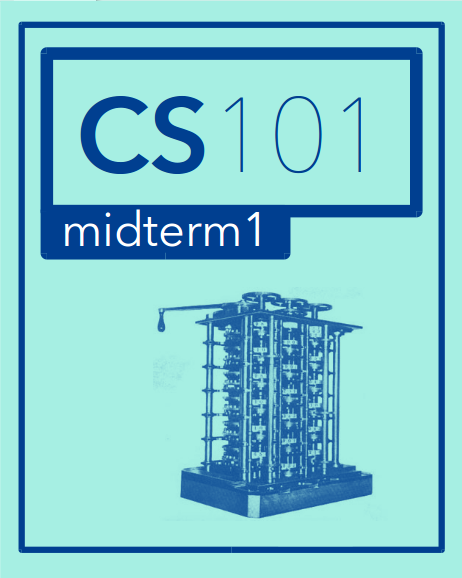
\includegraphics[width=2in]{../img/midterm1-header.png}
\end{center}

\bigskip
\noindent
\begin{itemize}
\item \textbf{Be sure to enter your \underline{NetID} and \underline{the code below} on your Scantron}.
\item Do not turn this page until instructed to do so.
\item There are 30 questions, worth 1 point each.
\item Each question has only \textbf{one} correct answer.
\item You must not communicate with other students during this test.
\item No books, notes, or electronic devices are permitted.
\item This is a 60-minute exam.
\item There are several different versions of this exam.
\end{itemize}

\bigskip\bigskip
\noindent
\textbf{\Large 1. Fill in your information:}

\bigskip
{\Large\bf
\begin{tabular}{ll}
Full Name: & \underbar{\hskip 8cm} \\[0.5em]
UIN (Student Number): & \underbar{\hskip 8cm} \\[0.5em]
NetID: & \underbar{\hskip 8cm}
\end{tabular}
}

\bigskip
\bigskip
\noindent
\textbf{\Large 2. Fill in the following answers on the Scantron form:}

%%%%%%%%%%%%%%%%%%%%%%%%%%%%%%%%%%%%%%%%%%%%%%%%%%%%%%%%%
%%%%%%%%%%%%%%%%%%%%%%%%%%%%%%%%%%%%%%%%%%%%%%%%%%%%%%%%%

\begin{enumerate}
\item[92.] B
\item[93.] A
\item[94.] B
\item[95.] A
\item[96.] B
\end{enumerate}

\newpage

% Zone 1


%%%%%%%%%%%%%%%%%%%%%%%%%%%%%%%%%%%%%%%%%%%%%%%%%%%%%%%%%



\newpage
\noindent
1. (1 point)
For this problem, you should compose a function which accomplishes a given task using the available code blocks arranged in the correct functional order.  \emph{We ignore indentation for this problem.}

\texttt{find\_max} should accept a \texttt{list} and return the value of the maximum item in the \texttt{list}.  (\texttt{None} is always the lowest value in any numeric comparison, so you may use it as an initializer.)

\begin{verbatim}
def find_max(my_list):
\end{verbatim}

\begin{enumerate}[1]
\item \texttt{max\_val = i}
\item \texttt{max\_val = None}
\item \texttt{for i in range(len(my\_list)):}
\item \texttt{if i > max\_val:}
\item \texttt{max\_val = my\_list[i]}
\item \texttt{return max\_val}
\item \texttt{for i in range(my\_list):}
\item \texttt{if my\_list[i] > max\_val:}
\item \texttt{print(max\_val)}
\end{enumerate}



\begin{enumerate}
\item[(A)]
2, 3, 4, 1, 6

\item[(B)] $\bigstar$ 
2, 3, 8, 5, 6

\item[(C)]
3, 2, 8, 5, 9

\item[(D)]
2, 7, 4, 5, 6

\item[(E)]
2, 3, 8, 1, 6

\end{enumerate}

\vspace*{2em}
\hrule
\vspace{2em}

\noindent {\bf Solution.} 
\vspace{2em}
\hrule height 2pt


\newpage
\noindent
2. (1 point)
Consider the following Python program.
\begin{verbatim}
e=[1,3,5,7,9,11]
d=[0,0,0]
for i in range(0,len(e)):
    d[i%3]+=e[i]
x=d[2]
\end{verbatim}
After it is run, what is the final \textbf{value} of \texttt{x}?


\begin{enumerate}
\item[(A)]
\begin{verbatim}8\end{verbatim}

\item[(B)]
\begin{verbatim}7\end{verbatim}

\item[(C)]
\begin{verbatim}0\end{verbatim}

\item[(D)] $\bigstar$ 
\begin{verbatim}16\end{verbatim}

\item[(E)]
\begin{verbatim}12\end{verbatim}

\end{enumerate}

\vspace*{2em}
\hrule
\vspace{2em}

\noindent {\bf Solution.} 
\vspace{2em}
\hrule height 2pt


\newpage
\noindent
3. (1 point)
Consider the following program:
\begin{verbatim}
x=[1,2,3,4,5,6,7,8,9]
x=x[2:-2]
i=1
while i < 3:
    x[i]+=1
    i+=1
\end{verbatim}
What is the \textbf{value} of \texttt{x} after this program is executed?


\begin{enumerate}
\item[(A)] $\bigstar$ 
\begin{verbatim}[3, 5, 6, 6, 7]\end{verbatim}

\item[(B)]
\begin{verbatim}[3, 5, 6, 6, 7, 8]\end{verbatim}

\item[(C)]
\begin{verbatim}[2, 4, 5, 5, 6, 7]\end{verbatim}

\item[(D)]
\begin{verbatim}[2, 4, 5, 6, 6, 7]\end{verbatim}

\item[(E)]
\begin{verbatim}[3, 5, 6, 6]\end{verbatim}

\end{enumerate}

\vspace*{2em}
\hrule
\vspace{2em}

\noindent {\bf Solution.} 
\vspace{2em}
\hrule height 2pt


\newpage
\noindent
4. (1 point)
Consider the following program.
\begin{verbatim}
s="ABCBA"
x=0
y=len(s)-1
while s[x]==s[y] and x<=y:
    x+=1
    y-=1
\end{verbatim}
After it is run, what is the final \textbf{value} of \texttt{x}?


\begin{enumerate}
\item[(A)] $\bigstar$ 
\begin{verbatim}3\end{verbatim}

\item[(B)]
\begin{verbatim}0\end{verbatim}

\item[(C)]
\begin{verbatim}4\end{verbatim}

\item[(D)]
\begin{verbatim}1\end{verbatim}

\item[(E)]
\begin{verbatim}2\end{verbatim}

\end{enumerate}

\vspace*{2em}
\hrule
\vspace{2em}

\noindent {\bf Solution.} 
\vspace{2em}
\hrule height 2pt


\newpage
\noindent
5. (1 point)
Consider the following program:
\begin{verbatim}
a=["merlin","sir agravaine","king pellinore"]
b=[ ]
for i in range(0,3):
    b.append(a[0-i].title())
\end{verbatim}
What is the \textbf{value} of b after this program is executed?


\begin{enumerate}
\item[(A)]
\begin{verbatim}[ ]\end{verbatim}

\item[(B)]
\begin{verbatim}['Sir Agravaine', 'King Pellinore']\end{verbatim}

\item[(C)]
\begin{verbatim}['King Pellinore', 'Sir Agravaine', 'Merlin']\end{verbatim}

\item[(D)] $\bigstar$ 
\begin{verbatim}['Merlin', 'King Pellinore', 'Sir Agravaine']\end{verbatim}

\item[(E)]
\begin{verbatim}['King Pellinore', 'Sir Agravaine']\end{verbatim}

\end{enumerate}

\vspace*{2em}
\hrule
\vspace{2em}

\noindent {\bf Solution.} 
\vspace{2em}
\hrule height 2pt


\newpage
\noindent
6. (1 point)
Consider the following program:
\begin{verbatim}
def fix(s):
    a=list(s)
    a.sort()
    return ''.join(a)

x=["one","two","eleven","twelve"]
s1=fix(x[0]+x[-1])
s2=fix(x[1]+x[-2])

if s1==s2:
    x.sort()
elif s1<s2:
    x.reverse()
else:
    x.append("six")
\end{verbatim}
What is the \textbf{value} of \texttt{x} after this program is executed?


\begin{enumerate}
\item[(A)]
\begin{verbatim}['two', 'twelve', 'one', 'eleven', 'six']\end{verbatim}

\item[(B)]
\begin{verbatim}['one', 'two', 'eleven', 'twelve', 'six']\end{verbatim}

\item[(C)]
\begin{verbatim}['one', 'two', 'eleven', 'twelve']\end{verbatim}

\item[(D)]
\begin{verbatim}['twelve', 'eleven', 'two', 'one']\end{verbatim}

\item[(E)] $\bigstar$ 
\begin{verbatim}['eleven', 'one', 'twelve', 'two']\end{verbatim}

\end{enumerate}

\vspace*{2em}
\hrule
\vspace{2em}

\noindent {\bf Solution.} 
\vspace{2em}
\hrule height 2pt


\newpage
\noindent
7. (1 point)
Consider the following program.
\begin{verbatim}
x=[]
for j in range(0,5):
    if (j%4)==0:
        x.append("-")
    if (j%5)==0:
        x.append("*")
\end{verbatim}
After it is run, what is the final \textbf{value} of \texttt{x}?


\begin{enumerate}
\item[(A)]
\begin{verbatim}["-","-","*"]\end{verbatim}

\item[(B)]
\begin{verbatim}["-","*","*"]\end{verbatim}

\item[(C)]
None of the other answers are correct.

\item[(D)]
\begin{verbatim}["-","*"]\end{verbatim}

\item[(E)] $\bigstar$ 
\begin{verbatim}["-","*","-"]\end{verbatim}

\end{enumerate}

\vspace*{2em}
\hrule
\vspace{2em}

\noindent {\bf Solution.} 
\vspace{2em}
\hrule height 2pt


\newpage
\noindent
8. (1 point)
Consider the following program:
\begin{verbatim}
s="-B-O-R-S-"
x=s.split("-")[2:-2]
\end{verbatim}
What is the \textbf{value} of \texttt{x} after this program is executed?


\begin{enumerate}
\item[(A)]
\begin{verbatim}None\end{verbatim}

\item[(B)]
\begin{verbatim}''\end{verbatim}

\item[(C)] $\bigstar$ 
\begin{verbatim}['O', 'R']\end{verbatim}

\item[(D)]
\begin{verbatim}False\end{verbatim}

\item[(E)]
\begin{verbatim}'ORS'\end{verbatim}

\end{enumerate}

\vspace*{2em}
\hrule
\vspace{2em}

\noindent {\bf Solution.} 
\vspace{2em}
\hrule height 2pt


\newpage
\noindent
9. (1 point)
Consider the following program:
\begin{verbatim}
x="KING ARTHUR-MORGANA LEFAY-SIR BEDIVERE".split("-")
y=x[:]
y.reverse()
\end{verbatim}
What is the \textbf{value} of \texttt{x} after this program is executed?


\begin{enumerate}
\item[(A)]
\begin{verbatim}['KING', 'ARTHUR-MORGANA', 'LEFAY-SIR', 'BEDIVERE']\end{verbatim}

\item[(B)]
\begin{verbatim}None\end{verbatim}

\item[(C)]
\begin{verbatim}['SIR BEDIVERE', 'MORGANA LEFAY', 'KING ARTHUR']\end{verbatim}

\item[(D)] $\bigstar$ 
\begin{verbatim}['KING ARTHUR', 'MORGANA LEFAY', 'SIR BEDIVERE']\end{verbatim}

\item[(E)]
\begin{verbatim}['BEDIVERE', 'LEFAY-SIR', 'ARTHUR-MORGANA', 'KING']\end{verbatim}

\end{enumerate}

\vspace*{2em}
\hrule
\vspace{2em}

\noindent {\bf Solution.} 
\vspace{2em}
\hrule height 2pt


\newpage
\noindent
10. (1 point)
Consider the following program:
\begin{verbatim}
i=2
x=3
while i < 7:
    x+=i
    i+=2
\end{verbatim}
What is the \textbf{value} of \texttt{x} after this program is executed?


\begin{enumerate}
\item[(A)]
\begin{verbatim}14\end{verbatim}

\item[(B)]
\begin{verbatim}11\end{verbatim}

\item[(C)]
\begin{verbatim}13\end{verbatim}

\item[(D)]
\begin{verbatim}12\end{verbatim}

\item[(E)] $\bigstar$ 
\begin{verbatim}15\end{verbatim}

\end{enumerate}

\vspace*{2em}
\hrule
\vspace{2em}

\noindent {\bf Solution.} 
\vspace{2em}
\hrule height 2pt


\newpage
\noindent
11. (1 point)
Consider the following program:
\begin{verbatim}
s="ECTOR"
t="GAWAIN"
x=(len(s)/(len(t)-1))+1
\end{verbatim}
What is the \textbf{type} of \texttt{x} after this program is executed?


\begin{enumerate}
\item[(A)]
\begin{verbatim}Boolean\end{verbatim}

\item[(B)] $\bigstar$ 
\begin{verbatim}Float\end{verbatim}

\item[(C)]
\begin{verbatim}String\end{verbatim}

\item[(D)]
\begin{verbatim}None\end{verbatim}

\item[(E)]
\begin{verbatim}Integer\end{verbatim}

\end{enumerate}

\vspace*{2em}
\hrule
\vspace{2em}

\noindent {\bf Solution.} 
\vspace{2em}
\hrule height 2pt


\newpage
\noindent
12. (1 point)
Evaluate the following expression:
\begin{verbatim}
[1,2]+[len("3")]
\end{verbatim}
What value is produced?


\begin{enumerate}
\item[(A)]
\begin{verbatim}[1,2,1,2,1,2]\end{verbatim}

\item[(B)]
\begin{verbatim}[1,2,"3"]\end{verbatim}

\item[(C)]
\begin{verbatim}[1,2,3]\end{verbatim}

\item[(D)] $\bigstar$ 
\begin{verbatim}[1,2,1]\end{verbatim}

\end{enumerate}

\vspace*{2em}
\hrule
\vspace{2em}

\noindent {\bf Solution.} 
\vspace{2em}
\hrule height 2pt


\newpage
\noindent
13. (1 point)
Consider the following program:
\begin{verbatim}
x=0
for i in range(4,10):
    if i%3==0:
        x+=3
    elif i%2==0:
        x+=2
    else:
        x+=1
\end{verbatim}
What is the \textbf{value} of \texttt{x} after this program is executed?


\begin{enumerate}
\item[(A)] $\bigstar$ 
\begin{verbatim}12\end{verbatim}

\item[(B)]
\begin{verbatim}14\end{verbatim}

\item[(C)]
\begin{verbatim}10\end{verbatim}

\item[(D)]
\begin{verbatim}13\end{verbatim}

\item[(E)]
\begin{verbatim}11\end{verbatim}

\end{enumerate}

\vspace*{2em}
\hrule
\vspace{2em}

\noindent {\bf Solution.} 
\vspace{2em}
\hrule height 2pt


\newpage
\noindent
14. (1 point)
Consider the following program.
\begin{verbatim}
kay = 2
wart = 3

def knight(kay,wart):
    wart += 2
    kay += 3
    return wart + kay

kay = knight(wart, kay) + knight(kay, wart)
\end{verbatim}
After it is run, what is the final \textbf{value} of \texttt{kay}?


\begin{enumerate}
\item[(A)]
\begin{verbatim}5\end{verbatim}

\item[(B)]
\begin{verbatim}3\end{verbatim}

\item[(C)] $\bigstar$ 
None of the other answers are correct.

\item[(D)]
\begin{verbatim}2\end{verbatim}

\end{enumerate}

\vspace*{2em}
\hrule
\vspace{2em}

\noindent {\bf Solution.} 
\vspace{2em}
\hrule height 2pt


\newpage
\noindent
15. (1 point)
Consider the following program:
\begin{verbatim}
s="TRIS %i"
t="ISEU"
x=len(s) % len(t[2:-1])
\end{verbatim}
What is the \textbf{type} of \texttt{x} after this program is executed?


\begin{enumerate}
\item[(A)]
\begin{verbatim}Float\end{verbatim}

\item[(B)]
\begin{verbatim}None\end{verbatim}

\item[(C)]
\begin{verbatim}String\end{verbatim}

\item[(D)]
\begin{verbatim}Boolean\end{verbatim}

\item[(E)] $\bigstar$ 
\begin{verbatim}Integer\end{verbatim}

\end{enumerate}

\vspace*{2em}
\hrule
\vspace{2em}

\noindent {\bf Solution.} 
\vspace{2em}
\hrule height 2pt


\newpage
\noindent
16. (1 point)
Consider the following program.
\begin{verbatim}
x=0
i=1
while(i*i)<=9:
    x=x+(i*i)
    i=i+1
\end{verbatim}
After it is run, what is the final \textbf{value} of \texttt{x}?


\begin{enumerate}
\item[(A)] $\bigstar$ 
\begin{verbatim}14\end{verbatim}

\item[(B)]
\begin{verbatim}5\end{verbatim}

\item[(C)]
\begin{verbatim}30\end{verbatim}

\item[(D)]
\begin{verbatim}3\end{verbatim}

\item[(E)]
\begin{verbatim}4\end{verbatim}

\end{enumerate}

\vspace*{2em}
\hrule
\vspace{2em}

\noindent {\bf Solution.} 
\vspace{2em}
\hrule height 2pt


\newpage
\noindent
17. (1 point)
Consider the following program:
\begin{verbatim}
a=3
b=4
if a!=b:
    a=b
elif a==4:
    a=5
else:
    b=a
\end{verbatim}
What is the \textbf{value} of a after this program is executed?


\begin{enumerate}
\item[(A)]
None of the other answers are correct.

\item[(B)]
\begin{verbatim}3\end{verbatim}

\item[(C)] $\bigstar$ 
\begin{verbatim}4\end{verbatim}

\item[(D)]
\begin{verbatim}5\end{verbatim}

\item[(E)]
\begin{verbatim}7\end{verbatim}

\end{enumerate}

\vspace*{2em}
\hrule
\vspace{2em}

\noindent {\bf Solution.} 
\vspace{2em}
\hrule height 2pt


\newpage
\noindent
18. (1 point)
Consider the following program:
\begin{verbatim}
x=[1,2,3]
def f(a):
    s=""
    a.append(4)
    for i in a:
        s+=str(i)
    return s

x.append(f(x))
\end{verbatim}
What is the \textbf{value} of \texttt{x} after this program is executed?


\begin{enumerate}
\item[(A)]
\begin{verbatim}[1, 2, 3, 10]\end{verbatim}

\item[(B)]
\begin{verbatim}[1, 2, 3, '123']\end{verbatim}

\item[(C)]
\begin{verbatim}[1, 2, 3, '1234']\end{verbatim}

\item[(D)] $\bigstar$ 
\begin{verbatim}[1, 2, 3, 4, '1234']\end{verbatim}

\item[(E)]
\begin{verbatim}[1, 2, 3]\end{verbatim}

\end{enumerate}

\vspace*{2em}
\hrule
\vspace{2em}

\noindent {\bf Solution.} 
\vspace{2em}
\hrule height 2pt


\newpage
\noindent
19. (1 point)
How can the following mathematical equation be implemented as a Python expression? Assume \verb|a|, \verb|b|, and \verb|cos| have already been defined.
$$a^b \cos(a - b)$$


\begin{enumerate}
\item[(A)]
\begin{verbatim}(a^b)*cos(a-b)\end{verbatim}

\item[(B)] $\bigstar$ 
\begin{verbatim}(a**b)*cos(a-b)\end{verbatim}

\item[(C)]
\begin{verbatim}(b^a)cos(a-b)\end{verbatim}

\item[(D)]
\begin{verbatim}(a**b)cos(a-b)\end{verbatim}

\item[(E)]
None of the other answers are correct.

\end{enumerate}

\vspace*{2em}
\hrule
\vspace{2em}

\noindent {\bf Solution.} 
\vspace{2em}
\hrule height 2pt


\newpage
\noindent
20. (1 point)
What is the result of the following expression?
\begin{verbatim}
[ 1, 2, 3 ] * 3.0
\end{verbatim}


\begin{enumerate}
\item[(A)]
\begin{verbatim}[1.0, 2.0, 3.0, 1.0, 2.0, 3.0, 1.0, 2.0, 3.0]\end{verbatim}

\item[(B)] $\bigstar$ 
\begin{verbatim}[1, 2, 3, 1, 2, 3, 1, 2, 3]\end{verbatim}

\item[(C)]
\begin{verbatim}[3.0, 6.0, 9.0]\end{verbatim}

\item[(D)]
\begin{verbatim}None of the above.\end{verbatim}

\item[(E)]
\begin{verbatim}[3, 6, 9]\end{verbatim}

\end{enumerate}

\vspace*{2em}
\hrule
\vspace{2em}

\noindent {\bf Solution.} 
\vspace{2em}
\hrule height 2pt


\newpage
\noindent
21. (1 point)
Consider the following program:
\begin{verbatim}
s="Calvin"
i=0
x=-1
while i<len(s):
    if s[i]=='b':
        x=i
    i+=1
\end{verbatim}
What is the \textbf{value} of \texttt{x} after this program is executed?


\begin{enumerate}
\item[(A)]
\begin{verbatim}3\end{verbatim}

\item[(B)]
\begin{verbatim}5\end{verbatim}

\item[(C)]
\begin{verbatim}6\end{verbatim}

\item[(D)]
\begin{verbatim}0\end{verbatim}

\item[(E)] $\bigstar$ 
\begin{verbatim}-1\end{verbatim}

\end{enumerate}

\vspace*{2em}
\hrule
\vspace{2em}

\noindent {\bf Solution.} 
\vspace{2em}
\hrule height 2pt


\newpage
\noindent
22. (1 point)
Consider the following program.
\begin{verbatim}
def artificing(s):
    return s*2
    return s+"%i" % 2
    return s

s=artificing("MERLIN")
\end{verbatim}
After it is run, what is the final \textbf{value} of s?


\begin{enumerate}
\item[(A)] $\bigstar$ 
\begin{verbatim}"MERLINMERLIN"\end{verbatim}

\item[(B)]
\begin{verbatim}"MERLIN"\end{verbatim}

\item[(C)]
\begin{verbatim}"MERLIN2"\end{verbatim}

\item[(D)]
\begin{verbatim}12\end{verbatim}

\item[(E)]
\begin{verbatim}None\end{verbatim}

\end{enumerate}

\vspace*{2em}
\hrule
\vspace{2em}

\noindent {\bf Solution.} 
\vspace{2em}
\hrule height 2pt


\newpage
\noindent
23. (1 point)
Consider the following incomplete function.
\begin{verbatim}
def ismultiple(m,n):
    if ???:
        return False
    else:
        return True
\end{verbatim}
The function is intended to return True if the input parameter m is a multiple of parameter n and False otherwise. For example, \verb|ismultiple(4,2)| should return \verb|True|, but \verb|ismultiple(5,3)| should return \verb|False|. What should replace the three question marks to complete the function?


\begin{enumerate}
\item[(A)]
\begin{verbatim}(m // n) != 0 \end{verbatim}

\item[(B)] $\bigstar$ 
\begin{verbatim}(m % n) != 0 \end{verbatim}

\item[(C)]
\begin{verbatim}(n // m) == 0 \end{verbatim}

\item[(D)]
\begin{verbatim}(n % m) == 0 \end{verbatim}

\end{enumerate}

\vspace*{2em}
\hrule
\vspace{2em}

\noindent {\bf Solution.} 
\vspace{2em}
\hrule height 2pt


\newpage
\noindent
24. (1 point)
Consider the following incomplete Python program.
\begin{verbatim}
s="".join(["1","0","2","1"])
x=0
for i in range(len(s)-1):
    x+=int(???)
\end{verbatim}
What should replace the three question marks so the resulting value of \texttt{x} is 33?


\begin{enumerate}
\item[(A)] $\bigstar$ 
\begin{verbatim}s[i:i+2]\end{verbatim}

\item[(B)]
\begin{verbatim}s[i:i+1]\end{verbatim}

\item[(C)]
\begin{verbatim}s[i+1:i+2]\end{verbatim}

\item[(D)]
\begin{verbatim}s[i:i-1]\end{verbatim}

\end{enumerate}

\vspace*{2em}
\hrule
\vspace{2em}

\noindent {\bf Solution.} 
\vspace{2em}
\hrule height 2pt


\newpage
\noindent
25. (1 point)
Consider the following incomplete program.
\begin{verbatim}
sum=0
for i in range(0,100):
    ???

\end{verbatim}
The program is intended to sum all of the integers between 1 and 100 (inclusive). What should replace the three question marks to complete the program?


\begin{enumerate}
\item[(A)]
\begin{verbatim}sum+1=sum \end{verbatim}

\item[(B)]
\begin{verbatim}sum=sum+i \end{verbatim}

\item[(C)]
\begin{verbatim}sum=sum+1\end{verbatim}

\item[(D)] $\bigstar$ 
\begin{verbatim}sum=sum+i+1 \end{verbatim}

\end{enumerate}

\vspace*{2em}
\hrule
\vspace{2em}

\noindent {\bf Solution.} 
\vspace{2em}
\hrule height 2pt


\newpage
\noindent
26. (1 point)
\begin{verbatim}
x=str(3)+"str(3)"
\end{verbatim}
What is the \textbf{value} of \texttt{x} after this program is executed?


\begin{enumerate}
\item[(A)]
\begin{verbatim}"33"\end{verbatim}

\item[(B)]
\begin{verbatim}"333"\end{verbatim}

\item[(C)]
\begin{verbatim}33\end{verbatim}

\item[(D)] $\bigstar$ 
\begin{verbatim}"3str(3)"\end{verbatim}

\item[(E)]
None of the other answers are correct.

\end{enumerate}

\vspace*{2em}
\hrule
\vspace{2em}

\noindent {\bf Solution.} 
\vspace{2em}
\hrule height 2pt


\newpage
\noindent
27. (1 point)
Evaluate the following expression:
\begin{verbatim}
len("ABCDE"[1:4])
\end{verbatim}
What value is produced?


\begin{enumerate}
\item[(A)] $\bigstar$ 
3

\item[(B)]
5

\item[(C)]
1

\item[(D)]
4

\end{enumerate}

\vspace*{2em}
\hrule
\vspace{2em}

\noindent {\bf Solution.} 
\vspace{2em}
\hrule height 2pt


\newpage
\noindent
28. (1 point)
Consider the following program:
\begin{verbatim}
a=["S","T","U","P","E","F","Y"]
a=a[0:4]
a.sort()
x=""
for e in a:
    x=e+x
\end{verbatim}
What is the \textbf{value} of \texttt{x} after this program is executed?


\begin{enumerate}
\item[(A)] $\bigstar$ 
\begin{verbatim}"UTSP"\end{verbatim}

\item[(B)]
None of the other answers are correct.

\item[(C)]
\begin{verbatim}"PUST"\end{verbatim}

\item[(D)]
\begin{verbatim}"STUP"\end{verbatim}

\item[(E)]
\begin{verbatim}"PSTU"\end{verbatim}

\end{enumerate}

\vspace*{2em}
\hrule
\vspace{2em}

\noindent {\bf Solution.} 
\vspace{2em}
\hrule height 2pt


\newpage
\noindent
29. (1 point)
Consider the following program:
\begin{verbatim}
x=3
a=7
if (a%3)==2:
    x=x**2
elif(a%3)==1:
    x=x**1
else:
    x=x**0
\end{verbatim}
What is the \textbf{value} of \texttt{x} after this program is executed?


\begin{enumerate}
\item[(A)]
None of the other answers are correct.

\item[(B)]
\begin{verbatim}1\end{verbatim}

\item[(C)] $\bigstar$ 
\begin{verbatim}3\end{verbatim}

\item[(D)]
\begin{verbatim}7\end{verbatim}

\item[(E)]
\begin{verbatim}9\end{verbatim}

\end{enumerate}

\vspace*{2em}
\hrule
\vspace{2em}

\noindent {\bf Solution.} 
\vspace{2em}
\hrule height 2pt


\newpage
\noindent
30. (1 point)
Consider the following program:
\begin{verbatim}
pi="3.14159"
e="2.71828"
x=pi*len(e)+pi
\end{verbatim}
What is the \textbf{type} of \texttt{x} after this program is executed?


\begin{enumerate}
\item[(A)]
\begin{verbatim}Float\end{verbatim}

\item[(B)]
\begin{verbatim}None\end{verbatim}

\item[(C)] $\bigstar$ 
\begin{verbatim}String\end{verbatim}

\item[(D)]
\begin{verbatim}Boolean\end{verbatim}

\item[(E)]
\begin{verbatim}Integer\end{verbatim}

\end{enumerate}

\vspace*{2em}
\hrule
\vspace{2em}

\noindent {\bf Solution.} 
\vspace{2em}
\hrule height 2pt

%%%%%%%%%%%%%%%%%%%%%%%%%%%%%%%%%%%%%%%%%%%%%%%%%%%%%%%%%%%%%%%%%%%%%%
%%%%%%%%%%%%%%%%%%%%%%%%%%%%%%%%%%%%%%%%%%%%%%%%%%%%%%%%%%%%%%%%%%%%%%
%%%%%%%%%%%%%%%%%%%%%%%%%%%%%%%%%%%%%%%%%%%%%%%%%%%%%%%%%%%%%%%%%%%%%%
%%%%%%%%%%%%%%%%%%%%%%%%%%%%%%%%%%%%%%%%%%%%%%%%%%%%%%%%%%%%%%%%%%%%%%
% Exam number 28

\message{Exam 28/50}
\cleardoublepage
\setcounter{page}{1}


\begin{center}
%\textbf{\Large CS 101 Midterm \#1}
%
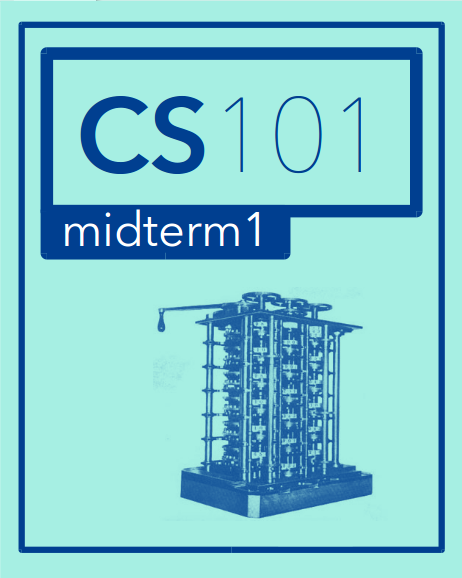
\includegraphics[width=2in]{../img/midterm1-header.png}
\end{center}

\bigskip
\noindent
\begin{itemize}
\item \textbf{Be sure to enter your \underline{NetID} and \underline{the code below} on your Scantron}.
\item Do not turn this page until instructed to do so.
\item There are 30 questions, worth 1 point each.
\item Each question has only \textbf{one} correct answer.
\item You must not communicate with other students during this test.
\item No books, notes, or electronic devices are permitted.
\item This is a 60-minute exam.
\item There are several different versions of this exam.
\end{itemize}

\bigskip\bigskip
\noindent
\textbf{\Large 1. Fill in your information:}

\bigskip
{\Large\bf
\begin{tabular}{ll}
Full Name: & \underbar{\hskip 8cm} \\[0.5em]
UIN (Student Number): & \underbar{\hskip 8cm} \\[0.5em]
NetID: & \underbar{\hskip 8cm}
\end{tabular}
}

\bigskip
\bigskip
\noindent
\textbf{\Large 2. Fill in the following answers on the Scantron form:}

%%%%%%%%%%%%%%%%%%%%%%%%%%%%%%%%%%%%%%%%%%%%%%%%%%%%%%%%%
%%%%%%%%%%%%%%%%%%%%%%%%%%%%%%%%%%%%%%%%%%%%%%%%%%%%%%%%%

\begin{enumerate}
\item[92.] C
\item[93.] A
\item[94.] B
\item[95.] B
\item[96.] C
\end{enumerate}

\newpage

% Zone 1


%%%%%%%%%%%%%%%%%%%%%%%%%%%%%%%%%%%%%%%%%%%%%%%%%%%%%%%%%



\newpage
\noindent
1. (1 point)
For this problem, you should compose a function which accomplishes a given task using the available code blocks arranged in the correct functional order.  \emph{We ignore indentation for this problem.}

\texttt{find\_max} should accept a \texttt{list} and return the value of the maximum item in the \texttt{list}.  (\texttt{None} is always the lowest value in any numeric comparison, so you may use it as an initializer.)

\begin{verbatim}
def find_max(my_list):
\end{verbatim}

\begin{enumerate}[1]
\item \texttt{max\_val = i}
\item \texttt{max\_val = None}
\item \texttt{for i in range(len(my\_list)):}
\item \texttt{if i > max\_val:}
\item \texttt{max\_val = my\_list[i]}
\item \texttt{return max\_val}
\item \texttt{for i in range(my\_list):}
\item \texttt{if my\_list[i] > max\_val:}
\item \texttt{print(max\_val)}
\end{enumerate}



\begin{enumerate}
\item[(A)] $\bigstar$ 
2, 3, 8, 5, 6

\item[(B)]
2, 3, 8, 1, 6

\item[(C)]
2, 3, 4, 1, 6

\item[(D)]
2, 7, 4, 5, 6

\item[(E)]
3, 2, 8, 5, 9

\end{enumerate}

\vspace*{2em}
\hrule
\vspace{2em}

\noindent {\bf Solution.} 
\vspace{2em}
\hrule height 2pt


\newpage
\noindent
2. (1 point)
Consider the following program:
\begin{verbatim}
def fix(s):
    a=list(s)
    a.sort()
    return ''.join(a)

x=["one","two","eleven","twelve"]
s1=fix(x[0]+x[-1])
s2=fix(x[1]+x[-2])

if s1<s2:
    x.sort()
elif s1==s2:
    x.reverse()
else:
    x.append("six")
\end{verbatim}
What is the \textbf{value} of \texttt{x} after this program is executed?


\begin{enumerate}
\item[(A)] $\bigstar$ 
\begin{verbatim}['twelve', 'eleven', 'two', 'one']\end{verbatim}

\item[(B)]
\begin{verbatim}['one', 'two', 'eleven', 'twelve']\end{verbatim}

\item[(C)]
\begin{verbatim}['two', 'twelve', 'one', 'eleven', 'six']\end{verbatim}

\item[(D)]
\begin{verbatim}['one', 'two', 'eleven', 'twelve', 'six']\end{verbatim}

\item[(E)]
\begin{verbatim}['eleven', 'one', 'twelve', 'two']\end{verbatim}

\end{enumerate}

\vspace*{2em}
\hrule
\vspace{2em}

\noindent {\bf Solution.} 
\vspace{2em}
\hrule height 2pt


\newpage
\noindent
3. (1 point)
Consider the following incomplete Python program.
\begin{verbatim}
s="".join(["1","0","2","1"])
x=0
for i in range(len(s)-1):
    x+=int(???)
\end{verbatim}
What should replace the three question marks so the resulting value of \texttt{x} is 33?


\begin{enumerate}
\item[(A)] $\bigstar$ 
\begin{verbatim}s[i:i+2]\end{verbatim}

\item[(B)]
\begin{verbatim}s[i+1:i+2]\end{verbatim}

\item[(C)]
\begin{verbatim}s[i:i+1]\end{verbatim}

\item[(D)]
\begin{verbatim}s[i:i-1]\end{verbatim}

\end{enumerate}

\vspace*{2em}
\hrule
\vspace{2em}

\noindent {\bf Solution.} 
\vspace{2em}
\hrule height 2pt


\newpage
\noindent
4. (1 point)
Consider the following program:
\begin{verbatim}
x=[1,2,3,4,5,6,7,8,9]
x=x[2:-2]
i=1
while i <= 3:
    x[i]+=1
    i+=1
\end{verbatim}
What is the \textbf{value} of \texttt{x} after this program is executed?


\begin{enumerate}
\item[(A)]
\begin{verbatim}[2, 4, 5, 5, 7, 7]\end{verbatim}

\item[(B)] $\bigstar$ 
\begin{verbatim}[3, 5, 6, 7, 7]\end{verbatim}

\item[(C)]
\begin{verbatim}[3, 5, 7, 7]\end{verbatim}

\item[(D)]
\begin{verbatim}[2, 4, 5, 6, 7, 7]\end{verbatim}

\item[(E)]
\begin{verbatim}[3, 5, 6, 7, 7, 8]\end{verbatim}

\end{enumerate}

\vspace*{2em}
\hrule
\vspace{2em}

\noindent {\bf Solution.} 
\vspace{2em}
\hrule height 2pt


\newpage
\noindent
5. (1 point)
Consider the following program.
\begin{verbatim}
x=[]
for j in range(0,5):
    if (j%4)==0:
        x.append("-")
    if (j%5)==0:
        x.append("*")
\end{verbatim}
After it is run, what is the final \textbf{value} of \texttt{x}?


\begin{enumerate}
\item[(A)]
\begin{verbatim}["-","*"]\end{verbatim}

\item[(B)]
None of the other answers are correct.

\item[(C)] $\bigstar$ 
\begin{verbatim}["-","*","-"]\end{verbatim}

\item[(D)]
\begin{verbatim}["-","-","*"]\end{verbatim}

\item[(E)]
\begin{verbatim}["-","*","*"]\end{verbatim}

\end{enumerate}

\vspace*{2em}
\hrule
\vspace{2em}

\noindent {\bf Solution.} 
\vspace{2em}
\hrule height 2pt


\newpage
\noindent
6. (1 point)
How can the following mathematical equation be implemented as a Python expression? Assume \verb|a|, \verb|b|, and \verb|sin| have already been defined.
$$a \sin(a^b - b)$$


\begin{enumerate}
\item[(A)]
\begin{verbatim}a*sin(b^a - b)\end{verbatim}

\item[(B)]
\begin{verbatim}a*sin(a^b - b)\end{verbatim}

\item[(C)] $\bigstar$ 
\begin{verbatim}a*sin(a**b - b)\end{verbatim}

\item[(D)]
None of the other answers are correct.

\item[(E)]
\begin{verbatim}a sin(a**b - b)\end{verbatim}

\end{enumerate}

\vspace*{2em}
\hrule
\vspace{2em}

\noindent {\bf Solution.} 
\vspace{2em}
\hrule height 2pt


\newpage
\noindent
7. (1 point)
Evaluate the following expression:
\begin{verbatim}
len("ABCD"[0:3])
\end{verbatim}
What value is produced?


\begin{enumerate}
\item[(A)] $\bigstar$ 
3

\item[(B)]
1

\item[(C)]
2

\item[(D)]
4

\end{enumerate}

\vspace*{2em}
\hrule
\vspace{2em}

\noindent {\bf Solution.} 
\vspace{2em}
\hrule height 2pt


\newpage
\noindent
8. (1 point)
Consider the following program:
\begin{verbatim}
x=[1,2,3]
def f(a):
    s=""
    a.reverse()
    for i in a:
        s+=str(i)
    return s

x.append(f(x))
\end{verbatim}
What is the \textbf{value} of \texttt{x} after this program is executed?


\begin{enumerate}
\item[(A)] $\bigstar$ 
\begin{verbatim}[3, 2, 1, '321']\end{verbatim}

\item[(B)]
\begin{verbatim}[3, 2, 1]\end{verbatim}

\item[(C)]
\begin{verbatim}[1, 2, 3]\end{verbatim}

\item[(D)]
\begin{verbatim}[1, 2, 3, '321']\end{verbatim}

\item[(E)]
\begin{verbatim}[1, 2, 3, 6]\end{verbatim}

\end{enumerate}

\vspace*{2em}
\hrule
\vspace{2em}

\noindent {\bf Solution.} 
\vspace{2em}
\hrule height 2pt


\newpage
\noindent
9. (1 point)
Consider the following program:
\begin{verbatim}
x=3
a=7
if (a%3)==2:
    x=x**2
elif(a%3)==1:
    x=x**1
else:
    x=x**0
\end{verbatim}
What is the \textbf{value} of \texttt{x} after this program is executed?


\begin{enumerate}
\item[(A)]
\begin{verbatim}7\end{verbatim}

\item[(B)]
None of the other answers are correct.

\item[(C)] $\bigstar$ 
\begin{verbatim}3\end{verbatim}

\item[(D)]
\begin{verbatim}1\end{verbatim}

\item[(E)]
\begin{verbatim}9\end{verbatim}

\end{enumerate}

\vspace*{2em}
\hrule
\vspace{2em}

\noindent {\bf Solution.} 
\vspace{2em}
\hrule height 2pt


\newpage
\noindent
10. (1 point)
Evaluate the following expression:
\begin{verbatim}
[1,2]+[len("3")]
\end{verbatim}
What value is produced?


\begin{enumerate}
\item[(A)]
\begin{verbatim}[1,2,"3"]\end{verbatim}

\item[(B)]
\begin{verbatim}[1,2,1,2,1,2]\end{verbatim}

\item[(C)]
\begin{verbatim}[1,2,3]\end{verbatim}

\item[(D)] $\bigstar$ 
\begin{verbatim}[1,2,1]\end{verbatim}

\end{enumerate}

\vspace*{2em}
\hrule
\vspace{2em}

\noindent {\bf Solution.} 
\vspace{2em}
\hrule height 2pt


\newpage
\noindent
11. (1 point)
Consider the following program.
\begin{verbatim}
s="ABCBA"
x=0
y=len(s)-1
while s[x]==s[y] and x<=y:
    x+=1
    y-=1
\end{verbatim}
After it is run, what is the final \textbf{value} of \texttt{x}?


\begin{enumerate}
\item[(A)]
\begin{verbatim}1\end{verbatim}

\item[(B)]
\begin{verbatim}0\end{verbatim}

\item[(C)] $\bigstar$ 
\begin{verbatim}3\end{verbatim}

\item[(D)]
\begin{verbatim}2\end{verbatim}

\item[(E)]
\begin{verbatim}4\end{verbatim}

\end{enumerate}

\vspace*{2em}
\hrule
\vspace{2em}

\noindent {\bf Solution.} 
\vspace{2em}
\hrule height 2pt


\newpage
\noindent
12. (1 point)
Consider the following program:
\begin{verbatim}
a=["merlin","sir agravaine","king pellinore"]
b=[ ]
for i in range(1,3):
    b.append(a[0-i].title())
\end{verbatim}
What is the \textbf{value} of b after this program is executed?


\begin{enumerate}
\item[(A)]
\begin{verbatim}[ ]\end{verbatim}

\item[(B)]
\begin{verbatim}['King Pellinore', 'Sir Agravaine', 'Merlin']\end{verbatim}

\item[(C)]
\begin{verbatim}['Sir Agravaine', 'King Pellinore']\end{verbatim}

\item[(D)] $\bigstar$ 
\begin{verbatim}['King Pellinore', 'Sir Agravaine']\end{verbatim}

\item[(E)]
\begin{verbatim}['Merlin', 'King Pellinore', 'Sir Agravaine']\end{verbatim}

\end{enumerate}

\vspace*{2em}
\hrule
\vspace{2em}

\noindent {\bf Solution.} 
\vspace{2em}
\hrule height 2pt


\newpage
\noindent
13. (1 point)
Consider the following program:
\begin{verbatim}
a=["S","T","U","P","E","F","Y"]
a=a[0:4]
a.sort()
x=""
for e in a:
    x=e+x
\end{verbatim}
What is the \textbf{value} of \texttt{x} after this program is executed?


\begin{enumerate}
\item[(A)]
\begin{verbatim}"PUST"\end{verbatim}

\item[(B)]
None of the other answers are correct.

\item[(C)] $\bigstar$ 
\begin{verbatim}"UTSP"\end{verbatim}

\item[(D)]
\begin{verbatim}"STUP"\end{verbatim}

\item[(E)]
\begin{verbatim}"PSTU"\end{verbatim}

\end{enumerate}

\vspace*{2em}
\hrule
\vspace{2em}

\noindent {\bf Solution.} 
\vspace{2em}
\hrule height 2pt


\newpage
\noindent
14. (1 point)
Consider the following program.
\begin{verbatim}
kay = 2
wart = 3

def knight(kay,wart):
    wart += 2
    kay += 3
    return wart + kay

wart = knight(kay, kay) + knight(wart, wart)
\end{verbatim}
After it is run, what is the final \textbf{value} of \texttt{wart}?


\begin{enumerate}
\item[(A)] $\bigstar$ 
None of the other answers are correct.

\item[(B)]
\begin{verbatim}3\end{verbatim}

\item[(C)]
\begin{verbatim}5\end{verbatim}

\item[(D)]
\begin{verbatim}2\end{verbatim}

\end{enumerate}

\vspace*{2em}
\hrule
\vspace{2em}

\noindent {\bf Solution.} 
\vspace{2em}
\hrule height 2pt


\newpage
\noindent
15. (1 point)
Consider the following program:
\begin{verbatim}
s="TRIS %i"
t="ISEU"
x=len(s) % len(t[2:-1])
\end{verbatim}
What is the \textbf{type} of \texttt{x} after this program is executed?


\begin{enumerate}
\item[(A)]
\begin{verbatim}Boolean\end{verbatim}

\item[(B)]
\begin{verbatim}None\end{verbatim}

\item[(C)]
\begin{verbatim}String\end{verbatim}

\item[(D)] $\bigstar$ 
\begin{verbatim}Integer\end{verbatim}

\item[(E)]
\begin{verbatim}Float\end{verbatim}

\end{enumerate}

\vspace*{2em}
\hrule
\vspace{2em}

\noindent {\bf Solution.} 
\vspace{2em}
\hrule height 2pt


\newpage
\noindent
16. (1 point)
Consider the following program:
\begin{verbatim}
s="ECTOR"
t="GAWAIN"
x=(len(s)+len(t)) < 4 and s in t
\end{verbatim}
What is the \textbf{type} of \texttt{x} after this program is executed?


\begin{enumerate}
\item[(A)]
\begin{verbatim}String\end{verbatim}

\item[(B)]
\begin{verbatim}Float\end{verbatim}

\item[(C)] $\bigstar$ 
\begin{verbatim}Boolean\end{verbatim}

\item[(D)]
\begin{verbatim}Integer\end{verbatim}

\item[(E)]
\begin{verbatim}None\end{verbatim}

\end{enumerate}

\vspace*{2em}
\hrule
\vspace{2em}

\noindent {\bf Solution.} 
\vspace{2em}
\hrule height 2pt


\newpage
\noindent
17. (1 point)
What is the result of the following expression?
\begin{verbatim}
[ 1, 2, 3 ] * 3.0
\end{verbatim}


\begin{enumerate}
\item[(A)]
\begin{verbatim}None of the above.\end{verbatim}

\item[(B)]
\begin{verbatim}[3, 6, 9]\end{verbatim}

\item[(C)]
\begin{verbatim}[3.0, 6.0, 9.0]\end{verbatim}

\item[(D)]
\begin{verbatim}[1.0, 2.0, 3.0, 1.0, 2.0, 3.0, 1.0, 2.0, 3.0]\end{verbatim}

\item[(E)] $\bigstar$ 
\begin{verbatim}[1, 2, 3, 1, 2, 3, 1, 2, 3]\end{verbatim}

\end{enumerate}

\vspace*{2em}
\hrule
\vspace{2em}

\noindent {\bf Solution.} 
\vspace{2em}
\hrule height 2pt


\newpage
\noindent
18. (1 point)
Consider the following program:
\begin{verbatim}
x=0
for i in range(2,7):
    if i%3==0:
        x+=3
    elif i%2==0:
        x+=2
    else:
        x+=1
\end{verbatim}
What is the \textbf{value} of \texttt{x} after this program is executed?


\begin{enumerate}
\item[(A)]
\begin{verbatim}14\end{verbatim}

\item[(B)] $\bigstar$ 
\begin{verbatim}11\end{verbatim}

\item[(C)]
\begin{verbatim}10\end{verbatim}

\item[(D)]
\begin{verbatim}12\end{verbatim}

\item[(E)]
\begin{verbatim}13\end{verbatim}

\end{enumerate}

\vspace*{2em}
\hrule
\vspace{2em}

\noindent {\bf Solution.} 
\vspace{2em}
\hrule height 2pt


\newpage
\noindent
19. (1 point)
Consider the following Python program.
\begin{verbatim}
e=[1,3,5,7,9,11]
d=[0,0,0]
for i in range(0,len(e)):
    d[i%3]+=e[i]
x=d[2]
\end{verbatim}
After it is run, what is the final \textbf{value} of \texttt{x}?


\begin{enumerate}
\item[(A)] $\bigstar$ 
\begin{verbatim}16\end{verbatim}

\item[(B)]
\begin{verbatim}7\end{verbatim}

\item[(C)]
\begin{verbatim}8\end{verbatim}

\item[(D)]
\begin{verbatim}0\end{verbatim}

\item[(E)]
\begin{verbatim}12\end{verbatim}

\end{enumerate}

\vspace*{2em}
\hrule
\vspace{2em}

\noindent {\bf Solution.} 
\vspace{2em}
\hrule height 2pt


\newpage
\noindent
20. (1 point)
Consider the following program:
\begin{verbatim}
s="-B-O-R-S-"
x=s.split("-")[2:-2]
\end{verbatim}
What is the \textbf{value} of \texttt{x} after this program is executed?


\begin{enumerate}
\item[(A)]
\begin{verbatim}''\end{verbatim}

\item[(B)]
\begin{verbatim}'ORS'\end{verbatim}

\item[(C)]
\begin{verbatim}None\end{verbatim}

\item[(D)] $\bigstar$ 
\begin{verbatim}['O', 'R']\end{verbatim}

\item[(E)]
\begin{verbatim}False\end{verbatim}

\end{enumerate}

\vspace*{2em}
\hrule
\vspace{2em}

\noindent {\bf Solution.} 
\vspace{2em}
\hrule height 2pt


\newpage
\noindent
21. (1 point)
Consider the following incomplete program.
\begin{verbatim}
sum=0
???:
    sum=sum+i

\end{verbatim}
The program is intended to sum all of the integers between 1 and 100 (inclusive). What should replace the three question marks to complete the program?


\begin{enumerate}
\item[(A)]
\begin{verbatim}while i<=100 \end{verbatim}

\item[(B)]
\begin{verbatim}for i in range(0,100)\end{verbatim}

\item[(C)]
\begin{verbatim}while i in range(100)\end{verbatim}

\item[(D)] $\bigstar$ 
\begin{verbatim}for i in range(1,101) \end{verbatim}

\end{enumerate}

\vspace*{2em}
\hrule
\vspace{2em}

\noindent {\bf Solution.} 
\vspace{2em}
\hrule height 2pt


\newpage
\noindent
22. (1 point)
Consider the following incomplete function.
\begin{verbatim}
def ismultiple(m,n):
    if ???:
        return False
    else:
        return True
\end{verbatim}
The function is intended to return True if the input parameter m is a multiple of parameter n and False otherwise. For example, \verb|ismultiple(4,2)| should return \verb|True|, but \verb|ismultiple(5,3)| should return \verb|False|. What should replace the three question marks to complete the function?


\begin{enumerate}
\item[(A)]
\begin{verbatim}(m // n) != 0 \end{verbatim}

\item[(B)]
\begin{verbatim}(n // m) == 0 \end{verbatim}

\item[(C)]
\begin{verbatim}(n % m) == 0 \end{verbatim}

\item[(D)] $\bigstar$ 
\begin{verbatim}(m % n) != 0 \end{verbatim}

\end{enumerate}

\vspace*{2em}
\hrule
\vspace{2em}

\noindent {\bf Solution.} 
\vspace{2em}
\hrule height 2pt


\newpage
\noindent
23. (1 point)
\begin{verbatim}
x=str(3)+"str(3)"
\end{verbatim}
What is the \textbf{value} of \texttt{x} after this program is executed?


\begin{enumerate}
\item[(A)]
\begin{verbatim}"33"\end{verbatim}

\item[(B)]
None of the other answers are correct.

\item[(C)]
\begin{verbatim}"333"\end{verbatim}

\item[(D)] $\bigstar$ 
\begin{verbatim}"3str(3)"\end{verbatim}

\item[(E)]
\begin{verbatim}33\end{verbatim}

\end{enumerate}

\vspace*{2em}
\hrule
\vspace{2em}

\noindent {\bf Solution.} 
\vspace{2em}
\hrule height 2pt


\newpage
\noindent
24. (1 point)
Consider the following program.
\begin{verbatim}
def artificing(s):
    return s+"%i" % 2
    return s*2
    return s

s=artificing("MERLIN")
\end{verbatim}
After it is run, what is the final \textbf{value} of s?


\begin{enumerate}
\item[(A)]
\begin{verbatim}"MERLIN%i"\end{verbatim}

\item[(B)]
\begin{verbatim}None\end{verbatim}

\item[(C)]
\begin{verbatim}0\end{verbatim}

\item[(D)] $\bigstar$ 
\begin{verbatim}"MERLIN2"\end{verbatim}

\item[(E)]
\begin{verbatim}"MERLINMERLIN"\end{verbatim}

\end{enumerate}

\vspace*{2em}
\hrule
\vspace{2em}

\noindent {\bf Solution.} 
\vspace{2em}
\hrule height 2pt


\newpage
\noindent
25. (1 point)
Consider the following program:
\begin{verbatim}
pi="3.14159"
e="2.71828"
x=pi*len(e)+pi
\end{verbatim}
What is the \textbf{type} of \texttt{x} after this program is executed?


\begin{enumerate}
\item[(A)]
\begin{verbatim}Integer\end{verbatim}

\item[(B)]
\begin{verbatim}None\end{verbatim}

\item[(C)]
\begin{verbatim}Float\end{verbatim}

\item[(D)]
\begin{verbatim}Boolean\end{verbatim}

\item[(E)] $\bigstar$ 
\begin{verbatim}String\end{verbatim}

\end{enumerate}

\vspace*{2em}
\hrule
\vspace{2em}

\noindent {\bf Solution.} 
\vspace{2em}
\hrule height 2pt


\newpage
\noindent
26. (1 point)
Consider the following program:
\begin{verbatim}
i=2
x=3
while i < 7:
    x+=i
    i+=2
\end{verbatim}
What is the \textbf{value} of \texttt{x} after this program is executed?


\begin{enumerate}
\item[(A)]
\begin{verbatim}12\end{verbatim}

\item[(B)]
\begin{verbatim}13\end{verbatim}

\item[(C)] $\bigstar$ 
\begin{verbatim}15\end{verbatim}

\item[(D)]
\begin{verbatim}14\end{verbatim}

\item[(E)]
\begin{verbatim}11\end{verbatim}

\end{enumerate}

\vspace*{2em}
\hrule
\vspace{2em}

\noindent {\bf Solution.} 
\vspace{2em}
\hrule height 2pt


\newpage
\noindent
27. (1 point)
Consider the following program:
\begin{verbatim}
a=3
b=4
if a!=b:
    a=b
elif a==4:
    a=5
else:
    b=a
\end{verbatim}
What is the \textbf{value} of a after this program is executed?


\begin{enumerate}
\item[(A)]
\begin{verbatim}5\end{verbatim}

\item[(B)]
None of the other answers are correct.

\item[(C)] $\bigstar$ 
\begin{verbatim}4\end{verbatim}

\item[(D)]
\begin{verbatim}3\end{verbatim}

\item[(E)]
\begin{verbatim}7\end{verbatim}

\end{enumerate}

\vspace*{2em}
\hrule
\vspace{2em}

\noindent {\bf Solution.} 
\vspace{2em}
\hrule height 2pt


\newpage
\noindent
28. (1 point)
Consider the following program:
\begin{verbatim}
x="KING ARTHUR-MORGANA LEFAY-SIR BEDIVERE".split("-")
y=x
y.reverse()
\end{verbatim}
What is the \textbf{value} of \texttt{x} after this program is executed?


\begin{enumerate}
\item[(A)]
\begin{verbatim}None\end{verbatim}

\item[(B)]
\begin{verbatim}['BEDIVERE', 'LEFAY-SIR', 'ARTHUR-MORGANA', 'KING']\end{verbatim}

\item[(C)]
\begin{verbatim}['KING ARTHUR', 'MORGANA LEFAY', 'SIR BEDIVERE']\end{verbatim}

\item[(D)] $\bigstar$ 
\begin{verbatim}['SIR BEDIVERE', 'MORGANA LEFAY', 'KING ARTHUR']\end{verbatim}

\item[(E)]
\begin{verbatim}['KING', 'ARTHUR-MORGANA', 'LEFAY-SIR', 'BEDIVERE']\end{verbatim}

\end{enumerate}

\vspace*{2em}
\hrule
\vspace{2em}

\noindent {\bf Solution.} 
\vspace{2em}
\hrule height 2pt


\newpage
\noindent
29. (1 point)
Consider the following program.
\begin{verbatim}
x=1
i=0
while(x*x)<=9:
    i=i+(x*x)
    x=x+1
\end{verbatim}
After it is run, what is the final \textbf{value} of \texttt{x}?


\begin{enumerate}
\item[(A)] $\bigstar$ 
\begin{verbatim}4\end{verbatim}

\item[(B)]
\begin{verbatim}3\end{verbatim}

\item[(C)]
\begin{verbatim}5\end{verbatim}

\item[(D)]
\begin{verbatim}30\end{verbatim}

\item[(E)]
\begin{verbatim}14\end{verbatim}

\end{enumerate}

\vspace*{2em}
\hrule
\vspace{2em}

\noindent {\bf Solution.} 
\vspace{2em}
\hrule height 2pt


\newpage
\noindent
30. (1 point)
Consider the following program:
\begin{verbatim}
s="Calvin"
i=0
x=-1
while i<len(s):
    if s[i]=='b':
        x=i
    i+=1
\end{verbatim}
What is the \textbf{value} of \texttt{x} after this program is executed?


\begin{enumerate}
\item[(A)]
\begin{verbatim}0\end{verbatim}

\item[(B)] $\bigstar$ 
\begin{verbatim}-1\end{verbatim}

\item[(C)]
\begin{verbatim}5\end{verbatim}

\item[(D)]
\begin{verbatim}3\end{verbatim}

\item[(E)]
\begin{verbatim}6\end{verbatim}

\end{enumerate}

\vspace*{2em}
\hrule
\vspace{2em}

\noindent {\bf Solution.} 
\vspace{2em}
\hrule height 2pt

%%%%%%%%%%%%%%%%%%%%%%%%%%%%%%%%%%%%%%%%%%%%%%%%%%%%%%%%%%%%%%%%%%%%%%
%%%%%%%%%%%%%%%%%%%%%%%%%%%%%%%%%%%%%%%%%%%%%%%%%%%%%%%%%%%%%%%%%%%%%%
%%%%%%%%%%%%%%%%%%%%%%%%%%%%%%%%%%%%%%%%%%%%%%%%%%%%%%%%%%%%%%%%%%%%%%
%%%%%%%%%%%%%%%%%%%%%%%%%%%%%%%%%%%%%%%%%%%%%%%%%%%%%%%%%%%%%%%%%%%%%%
% Exam number 29

\message{Exam 29/50}
\cleardoublepage
\setcounter{page}{1}


\begin{center}
%\textbf{\Large CS 101 Midterm \#1}
%
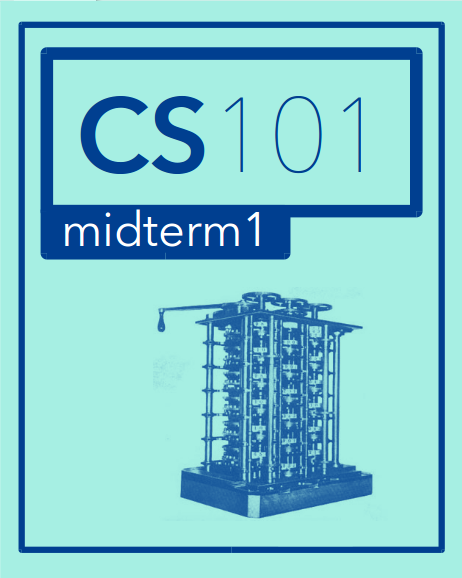
\includegraphics[width=2in]{../img/midterm1-header.png}
\end{center}

\bigskip
\noindent
\begin{itemize}
\item \textbf{Be sure to enter your \underline{NetID} and \underline{the code below} on your Scantron}.
\item Do not turn this page until instructed to do so.
\item There are 30 questions, worth 1 point each.
\item Each question has only \textbf{one} correct answer.
\item You must not communicate with other students during this test.
\item No books, notes, or electronic devices are permitted.
\item This is a 60-minute exam.
\item There are several different versions of this exam.
\end{itemize}

\bigskip\bigskip
\noindent
\textbf{\Large 1. Fill in your information:}

\bigskip
{\Large\bf
\begin{tabular}{ll}
Full Name: & \underbar{\hskip 8cm} \\[0.5em]
UIN (Student Number): & \underbar{\hskip 8cm} \\[0.5em]
NetID: & \underbar{\hskip 8cm}
\end{tabular}
}

\bigskip
\bigskip
\noindent
\textbf{\Large 2. Fill in the following answers on the Scantron form:}

%%%%%%%%%%%%%%%%%%%%%%%%%%%%%%%%%%%%%%%%%%%%%%%%%%%%%%%%%
%%%%%%%%%%%%%%%%%%%%%%%%%%%%%%%%%%%%%%%%%%%%%%%%%%%%%%%%%

\begin{enumerate}
\item[92.] D
\item[93.] A
\item[94.] B
\item[95.] C
\item[96.] D
\end{enumerate}

\newpage

% Zone 1


%%%%%%%%%%%%%%%%%%%%%%%%%%%%%%%%%%%%%%%%%%%%%%%%%%%%%%%%%



\newpage
\noindent
1. (1 point)
Consider the following program:
\begin{verbatim}
pi="3.14159"
e="2.71828"
x=(float(e)**float(pi)-float(pi)) == 20
\end{verbatim}
What is the \textbf{type} of \texttt{x} after this program is executed?


\begin{enumerate}
\item[(A)]
\begin{verbatim}None\end{verbatim}

\item[(B)]
\begin{verbatim}Float\end{verbatim}

\item[(C)]
\begin{verbatim}Integer\end{verbatim}

\item[(D)] $\bigstar$ 
\begin{verbatim}Boolean\end{verbatim}

\item[(E)]
\begin{verbatim}String\end{verbatim}

\end{enumerate}

\vspace*{2em}
\hrule
\vspace{2em}

\noindent {\bf Solution.} 
\vspace{2em}
\hrule height 2pt


\newpage
\noindent
2. (1 point)
Consider the following program:
\begin{verbatim}
s="TRIS %i"
t="ISEU"
x=s % len(t)
\end{verbatim}
What is the \textbf{type} of \texttt{x} after this program is executed?


\begin{enumerate}
\item[(A)] $\bigstar$ 
\begin{verbatim}String\end{verbatim}

\item[(B)]
\begin{verbatim}None\end{verbatim}

\item[(C)]
\begin{verbatim}Integer\end{verbatim}

\item[(D)]
\begin{verbatim}Boolean\end{verbatim}

\item[(E)]
\begin{verbatim}Float\end{verbatim}

\end{enumerate}

\vspace*{2em}
\hrule
\vspace{2em}

\noindent {\bf Solution.} 
\vspace{2em}
\hrule height 2pt


\newpage
\noindent
3. (1 point)
Evaluate the following expression:
\begin{verbatim}
[1,2]*len("3")
\end{verbatim}
What value is produced?


\begin{enumerate}
\item[(A)]
\begin{verbatim}[1,2,3]\end{verbatim}

\item[(B)] $\bigstar$ 
\begin{verbatim}[1,2]\end{verbatim}

\item[(C)]
\begin{verbatim}[1,2,1]\end{verbatim}

\item[(D)]
\begin{verbatim}[1,2,1,2,1,2]\end{verbatim}

\end{enumerate}

\vspace*{2em}
\hrule
\vspace{2em}

\noindent {\bf Solution.} 
\vspace{2em}
\hrule height 2pt


\newpage
\noindent
4. (1 point)
Consider the following program:
\begin{verbatim}
s="Calvin"
i=0
x=-1
while i<len(s):
    if s[i]=='b':
        x=i
    i+=1
\end{verbatim}
What is the \textbf{value} of \texttt{x} after this program is executed?


\begin{enumerate}
\item[(A)]
\begin{verbatim}0\end{verbatim}

\item[(B)]
\begin{verbatim}6\end{verbatim}

\item[(C)] $\bigstar$ 
\begin{verbatim}-1\end{verbatim}

\item[(D)]
\begin{verbatim}3\end{verbatim}

\item[(E)]
\begin{verbatim}5\end{verbatim}

\end{enumerate}

\vspace*{2em}
\hrule
\vspace{2em}

\noindent {\bf Solution.} 
\vspace{2em}
\hrule height 2pt


\newpage
\noindent
5. (1 point)
Consider the following program:
\begin{verbatim}
x=[2,3,4,5,6,7,8,9]
x=x[2:-2]
i=1
while i <= 3:
    x[i]+=1
    i+=1
\end{verbatim}
What is the \textbf{value} of \texttt{x} after this program is executed?


\begin{enumerate}
\item[(A)]
\begin{verbatim}[4, 6, 7]\end{verbatim}

\item[(B)]
\begin{verbatim}[2, 4, 6, 6]\end{verbatim}

\item[(C)]
\begin{verbatim}[4, 6, 7, 7]\end{verbatim}

\item[(D)] $\bigstar$ 
\begin{verbatim}[4, 6, 7, 8]\end{verbatim}

\item[(E)]
\begin{verbatim}[3, 4, 6, 7, 8]\end{verbatim}

\end{enumerate}

\vspace*{2em}
\hrule
\vspace{2em}

\noindent {\bf Solution.} 
\vspace{2em}
\hrule height 2pt


\newpage
\noindent
6. (1 point)
Consider the following program.
\begin{verbatim}
x=[]
for j in range(0,5):
    if (j%2)==0:
        x.append("-")
    if (j%5)==0:
        x.append("*")
\end{verbatim}
After it is run, what is the final \textbf{value} of \texttt{x}?


\begin{enumerate}
\item[(A)]
\begin{verbatim}["-","*","-"]\end{verbatim}

\item[(B)]
\begin{verbatim}["*","-","*","*"]\end{verbatim}

\item[(C)] $\bigstar$ 
\begin{verbatim}["-","*","-","-"]\end{verbatim}

\item[(D)]
\begin{verbatim}["-","-","*"]\end{verbatim}

\item[(E)]
None of the other answers are correct.

\end{enumerate}

\vspace*{2em}
\hrule
\vspace{2em}

\noindent {\bf Solution.} 
\vspace{2em}
\hrule height 2pt


\newpage
\noindent
7. (1 point)
\begin{verbatim}
x=str(3)+"str(3)"
\end{verbatim}
What is the \textbf{value} of \texttt{x} after this program is executed?


\begin{enumerate}
\item[(A)]
\begin{verbatim}"333"\end{verbatim}

\item[(B)]
\begin{verbatim}"33"\end{verbatim}

\item[(C)] $\bigstar$ 
\begin{verbatim}"3str(3)"\end{verbatim}

\item[(D)]
\begin{verbatim}33\end{verbatim}

\item[(E)]
None of the other answers are correct.

\end{enumerate}

\vspace*{2em}
\hrule
\vspace{2em}

\noindent {\bf Solution.} 
\vspace{2em}
\hrule height 2pt


\newpage
\noindent
8. (1 point)
Consider the following program:
\begin{verbatim}
x=[1,2,3]
def f(a):
    s=""
    a.reverse()
    for i in a:
        s+=str(i)
    return s

x.append(f(x))
\end{verbatim}
What is the \textbf{value} of \texttt{x} after this program is executed?


\begin{enumerate}
\item[(A)]
\begin{verbatim}[1, 2, 3]\end{verbatim}

\item[(B)]
\begin{verbatim}[3, 2, 1]\end{verbatim}

\item[(C)] $\bigstar$ 
\begin{verbatim}[3, 2, 1, '321']\end{verbatim}

\item[(D)]
\begin{verbatim}[1, 2, 3, '321']\end{verbatim}

\item[(E)]
\begin{verbatim}[1, 2, 3, 6]\end{verbatim}

\end{enumerate}

\vspace*{2em}
\hrule
\vspace{2em}

\noindent {\bf Solution.} 
\vspace{2em}
\hrule height 2pt


\newpage
\noindent
9. (1 point)
Consider the following program:
\begin{verbatim}
x=0
for i in range(2,7):
    if i%3==0:
        x+=3
    elif i%2==0:
        x+=2
    else:
        x+=1
\end{verbatim}
What is the \textbf{value} of \texttt{x} after this program is executed?


\begin{enumerate}
\item[(A)] $\bigstar$ 
\begin{verbatim}11\end{verbatim}

\item[(B)]
\begin{verbatim}13\end{verbatim}

\item[(C)]
\begin{verbatim}10\end{verbatim}

\item[(D)]
\begin{verbatim}12\end{verbatim}

\item[(E)]
\begin{verbatim}14\end{verbatim}

\end{enumerate}

\vspace*{2em}
\hrule
\vspace{2em}

\noindent {\bf Solution.} 
\vspace{2em}
\hrule height 2pt


\newpage
\noindent
10. (1 point)
Consider the following program:
\begin{verbatim}
i=2
x=3
while i < 7:
    x+=i
    i+=2
\end{verbatim}
What is the \textbf{value} of \texttt{x} after this program is executed?


\begin{enumerate}
\item[(A)]
\begin{verbatim}12\end{verbatim}

\item[(B)]
\begin{verbatim}11\end{verbatim}

\item[(C)] $\bigstar$ 
\begin{verbatim}15\end{verbatim}

\item[(D)]
\begin{verbatim}13\end{verbatim}

\item[(E)]
\begin{verbatim}14\end{verbatim}

\end{enumerate}

\vspace*{2em}
\hrule
\vspace{2em}

\noindent {\bf Solution.} 
\vspace{2em}
\hrule height 2pt


\newpage
\noindent
11. (1 point)
Consider the following program.
\begin{verbatim}
x=1
i=0
while(x*x)<=9:
    i=i+(x*x)
    x=x+1
\end{verbatim}
After it is run, what is the final \textbf{value} of \texttt{x}?


\begin{enumerate}
\item[(A)] $\bigstar$ 
\begin{verbatim}4\end{verbatim}

\item[(B)]
\begin{verbatim}30\end{verbatim}

\item[(C)]
\begin{verbatim}3\end{verbatim}

\item[(D)]
\begin{verbatim}5\end{verbatim}

\item[(E)]
\begin{verbatim}14\end{verbatim}

\end{enumerate}

\vspace*{2em}
\hrule
\vspace{2em}

\noindent {\bf Solution.} 
\vspace{2em}
\hrule height 2pt


\newpage
\noindent
12. (1 point)
Consider the following program:
\begin{verbatim}
s="-B-O-R-S-"
x=s.split("-")[2:-2]
\end{verbatim}
What is the \textbf{value} of \texttt{x} after this program is executed?


\begin{enumerate}
\item[(A)]
\begin{verbatim}'ORS'\end{verbatim}

\item[(B)] $\bigstar$ 
\begin{verbatim}['O', 'R']\end{verbatim}

\item[(C)]
\begin{verbatim}False\end{verbatim}

\item[(D)]
\begin{verbatim}''\end{verbatim}

\item[(E)]
\begin{verbatim}None\end{verbatim}

\end{enumerate}

\vspace*{2em}
\hrule
\vspace{2em}

\noindent {\bf Solution.} 
\vspace{2em}
\hrule height 2pt


\newpage
\noindent
13. (1 point)
Consider the following program.
\begin{verbatim}
s="ABCBA"
x=0
y=len(s)-1
while s[x]==s[y] and x<=y:
    x+=1
    y-=1
\end{verbatim}
After it is run, what is the final \textbf{value} of \texttt{x}?


\begin{enumerate}
\item[(A)] $\bigstar$ 
\begin{verbatim}3\end{verbatim}

\item[(B)]
\begin{verbatim}1\end{verbatim}

\item[(C)]
\begin{verbatim}2\end{verbatim}

\item[(D)]
\begin{verbatim}4\end{verbatim}

\item[(E)]
\begin{verbatim}0\end{verbatim}

\end{enumerate}

\vspace*{2em}
\hrule
\vspace{2em}

\noindent {\bf Solution.} 
\vspace{2em}
\hrule height 2pt


\newpage
\noindent
14. (1 point)
Consider the following program.
\begin{verbatim}
kay = 2
wart = 3

def knight(kay,wart):
    wart += 2
    kay += 3
    return wart + kay

wart = knight(kay, kay) + knight(wart, wart)
\end{verbatim}
After it is run, what is the final \textbf{value} of \texttt{wart}?


\begin{enumerate}
\item[(A)]
\begin{verbatim}5\end{verbatim}

\item[(B)]
\begin{verbatim}3\end{verbatim}

\item[(C)]
\begin{verbatim}2\end{verbatim}

\item[(D)] $\bigstar$ 
None of the other answers are correct.

\end{enumerate}

\vspace*{2em}
\hrule
\vspace{2em}

\noindent {\bf Solution.} 
\vspace{2em}
\hrule height 2pt


\newpage
\noindent
15. (1 point)
Consider the following program:
\begin{verbatim}
x=3
a=5
if (a%3)==2:
    x=x**3
elif(a%3)==1:
    x=x**2
else:
    x=x**1
\end{verbatim}
What is the \textbf{value} of \texttt{x} after this program is executed?


\begin{enumerate}
\item[(A)] $\bigstar$ 
\begin{verbatim}27\end{verbatim}

\item[(B)]
None of the other answers are correct.

\item[(C)]
\begin{verbatim}1\end{verbatim}

\item[(D)]
\begin{verbatim}9\end{verbatim}

\item[(E)]
\begin{verbatim}3\end{verbatim}

\end{enumerate}

\vspace*{2em}
\hrule
\vspace{2em}

\noindent {\bf Solution.} 
\vspace{2em}
\hrule height 2pt


\newpage
\noindent
16. (1 point)
Consider the following incomplete function.
\begin{verbatim}
def isdivisible(m,n):
    if ???:
        return False
    else:
        return True
\end{verbatim}
The function is intended to return True if the input parameter m is evenly divisible by the parameter n and False otherwise. For example, \verb|isdivisible(4,2)| should return \verb|True|, but \verb|isdivisible(5,3)| should return \verb|False|. What should replace the three question marks to complete the function?


\begin{enumerate}
\item[(A)]
\begin{verbatim}(n // m) == 0 \end{verbatim}

\item[(B)]
\begin{verbatim}(m // n) != 0 \end{verbatim}

\item[(C)]
\begin{verbatim}(n % m) == 0 \end{verbatim}

\item[(D)] $\bigstar$ 
\begin{verbatim}(m % n) != 0 \end{verbatim}

\end{enumerate}

\vspace*{2em}
\hrule
\vspace{2em}

\noindent {\bf Solution.} 
\vspace{2em}
\hrule height 2pt


\newpage
\noindent
17. (1 point)
Consider the following Python program.
\begin{verbatim}
e=[1,3,5,7,9,11]
d=[0,0,0]
for i in range(0,len(e)):
    d[i%3]+=e[i]
x=d[2]
\end{verbatim}
After it is run, what is the final \textbf{value} of \texttt{x}?


\begin{enumerate}
\item[(A)]
\begin{verbatim}0\end{verbatim}

\item[(B)]
\begin{verbatim}7\end{verbatim}

\item[(C)]
\begin{verbatim}12\end{verbatim}

\item[(D)] $\bigstar$ 
\begin{verbatim}16\end{verbatim}

\item[(E)]
\begin{verbatim}8\end{verbatim}

\end{enumerate}

\vspace*{2em}
\hrule
\vspace{2em}

\noindent {\bf Solution.} 
\vspace{2em}
\hrule height 2pt


\newpage
\noindent
18. (1 point)
Consider the following incomplete program.
\begin{verbatim}
sum=0
for i in range(0,100):
    ???

\end{verbatim}
The program is intended to sum all of the integers between 1 and 100 (inclusive). What should replace the three question marks to complete the program?


\begin{enumerate}
\item[(A)] $\bigstar$ 
\begin{verbatim}sum=sum+i+1 \end{verbatim}

\item[(B)]
\begin{verbatim}sum=sum+1\end{verbatim}

\item[(C)]
\begin{verbatim}sum+1=sum \end{verbatim}

\item[(D)]
\begin{verbatim}sum=sum+i \end{verbatim}

\end{enumerate}

\vspace*{2em}
\hrule
\vspace{2em}

\noindent {\bf Solution.} 
\vspace{2em}
\hrule height 2pt


\newpage
\noindent
19. (1 point)
Evaluate the following expression:
\begin{verbatim}
len("ABCD"[0:3])
\end{verbatim}
What value is produced?


\begin{enumerate}
\item[(A)]
2

\item[(B)] $\bigstar$ 
3

\item[(C)]
1

\item[(D)]
4

\end{enumerate}

\vspace*{2em}
\hrule
\vspace{2em}

\noindent {\bf Solution.} 
\vspace{2em}
\hrule height 2pt


\newpage
\noindent
20. (1 point)
Consider the following program:
\begin{verbatim}
x="KING ARTHUR-MORGANA LEFAY-SIR BEDIVERE".split("-")
y=x
x=y.reverse()
\end{verbatim}
What is the \textbf{value} of \texttt{x} after this program is executed?


\begin{enumerate}
\item[(A)]
\begin{verbatim}['BEDIVERE', 'LEFAY-SIR', 'ARTHUR-MORGANA', 'KING']\end{verbatim}

\item[(B)]
\begin{verbatim}['SIR BEDIVERE', 'MORGANA LEFAY', 'KING ARTHUR']\end{verbatim}

\item[(C)] $\bigstar$ 
\begin{verbatim}None\end{verbatim}

\item[(D)]
\begin{verbatim}['KING', 'ARTHUR-MORGANA', 'LEFAY-SIR', 'BEDIVERE']\end{verbatim}

\item[(E)]
\begin{verbatim}['KING ARTHUR', 'MORGANA LEFAY', 'SIR BEDIVERE']\end{verbatim}

\end{enumerate}

\vspace*{2em}
\hrule
\vspace{2em}

\noindent {\bf Solution.} 
\vspace{2em}
\hrule height 2pt


\newpage
\noindent
21. (1 point)
Consider the following program:
\begin{verbatim}
a=3
b=4
if a!=b:
    a=b
elif a==4:
    a=5
else:
    b=a
\end{verbatim}
What is the \textbf{value} of a after this program is executed?


\begin{enumerate}
\item[(A)] $\bigstar$ 
\begin{verbatim}4\end{verbatim}

\item[(B)]
\begin{verbatim}7\end{verbatim}

\item[(C)]
None of the other answers are correct.

\item[(D)]
\begin{verbatim}3\end{verbatim}

\item[(E)]
\begin{verbatim}5\end{verbatim}

\end{enumerate}

\vspace*{2em}
\hrule
\vspace{2em}

\noindent {\bf Solution.} 
\vspace{2em}
\hrule height 2pt


\newpage
\noindent
22. (1 point)
Consider the following program:
\begin{verbatim}
a=["merlin","sir agravaine","king pellinore"]
b=[ ]
for i in range(0,3):
    b.append(a[0-i].title())
\end{verbatim}
What is the \textbf{value} of b after this program is executed?


\begin{enumerate}
\item[(A)] $\bigstar$ 
\begin{verbatim}['Merlin', 'King Pellinore', 'Sir Agravaine']\end{verbatim}

\item[(B)]
\begin{verbatim}['Sir Agravaine', 'King Pellinore']\end{verbatim}

\item[(C)]
\begin{verbatim}[ ]\end{verbatim}

\item[(D)]
\begin{verbatim}['King Pellinore', 'Sir Agravaine', 'Merlin']\end{verbatim}

\item[(E)]
\begin{verbatim}['King Pellinore', 'Sir Agravaine']\end{verbatim}

\end{enumerate}

\vspace*{2em}
\hrule
\vspace{2em}

\noindent {\bf Solution.} 
\vspace{2em}
\hrule height 2pt


\newpage
\noindent
23. (1 point)
Consider the following program:
\begin{verbatim}
a=["A","C","C","I","O"]
a.sort()
a[0]=a[-1]
x=""
for e in a:
    x=x+e
\end{verbatim}
What is the \textbf{value} of \texttt{x} after this program is executed?


\begin{enumerate}
\item[(A)]
\begin{verbatim}"ACCIA"\end{verbatim}

\item[(B)]
\begin{verbatim}"ICCOI"\end{verbatim}

\item[(C)]
\begin{verbatim}"ACCOA"\end{verbatim}

\item[(D)] $\bigstar$ 
\begin{verbatim}"OCCIO"\end{verbatim}

\item[(E)]
None of the other answers are correct.

\end{enumerate}

\vspace*{2em}
\hrule
\vspace{2em}

\noindent {\bf Solution.} 
\vspace{2em}
\hrule height 2pt


\newpage
\noindent
24. (1 point)
Consider the following incomplete Python program.
\begin{verbatim}
s="".join(["1","0","2","1"])
x=0
for i in range(len(s)-1):
    x+=int(???)
\end{verbatim}
What should replace the three question marks so the resulting value of \texttt{x} is 33?


\begin{enumerate}
\item[(A)]
\begin{verbatim}s[i+1:i+2]\end{verbatim}

\item[(B)] $\bigstar$ 
\begin{verbatim}s[i:i+2]\end{verbatim}

\item[(C)]
\begin{verbatim}s[i:i-1]\end{verbatim}

\item[(D)]
\begin{verbatim}s[i:i+1]\end{verbatim}

\end{enumerate}

\vspace*{2em}
\hrule
\vspace{2em}

\noindent {\bf Solution.} 
\vspace{2em}
\hrule height 2pt


\newpage
\noindent
25. (1 point)
How can the following mathematical equation be implemented as a Python expression? Assume \verb|a|, \verb|b|, and \verb|cos| have already been defined.
$$a^b \cos(a - b)$$


\begin{enumerate}
\item[(A)]
\begin{verbatim}(a^b)*cos(a-b)\end{verbatim}

\item[(B)] $\bigstar$ 
\begin{verbatim}(a**b)*cos(a-b)\end{verbatim}

\item[(C)]
\begin{verbatim}(a**b)cos(a-b)\end{verbatim}

\item[(D)]
\begin{verbatim}(b^a)cos(a-b)\end{verbatim}

\item[(E)]
None of the other answers are correct.

\end{enumerate}

\vspace*{2em}
\hrule
\vspace{2em}

\noindent {\bf Solution.} 
\vspace{2em}
\hrule height 2pt


\newpage
\noindent
26. (1 point)
For this problem, you should compose a function which accomplishes a given task using the available code blocks arranged in the correct functional order.  \emph{We ignore indentation for this problem.}

\texttt{find\_max} should accept a \texttt{list} and return the value of the maximum item in the \texttt{list}.  (\texttt{None} is always the lowest value in any numeric comparison, so you may use it as an initializer.)

\begin{verbatim}
def find_max(my_list):
\end{verbatim}

\begin{enumerate}[1]
\item \texttt{max\_val = i}
\item \texttt{max\_val = None}
\item \texttt{for i in range(len(my\_list)):}
\item \texttt{if i > max\_val:}
\item \texttt{max\_val = my\_list[i]}
\item \texttt{return max\_val}
\item \texttt{for i in range(my\_list):}
\item \texttt{if my\_list[i] > max\_val:}
\item \texttt{print(max\_val)}
\end{enumerate}



\begin{enumerate}
\item[(A)] $\bigstar$ 
2, 3, 8, 5, 6

\item[(B)]
2, 3, 4, 1, 6

\item[(C)]
2, 3, 8, 1, 6

\item[(D)]
2, 7, 4, 5, 6

\item[(E)]
3, 2, 8, 5, 9

\end{enumerate}

\vspace*{2em}
\hrule
\vspace{2em}

\noindent {\bf Solution.} 
\vspace{2em}
\hrule height 2pt


\newpage
\noindent
27. (1 point)
Consider the following program:
\begin{verbatim}
def fix(s):
    a=list(s)
    a.sort()
    return ''.join(a)

x=["one","two","eleven","twelve"]
s1=fix(x[0]+x[-1])
s2=fix(x[1]+x[-2])

if s1==s2:
    x.sort()
elif s1<s2:
    x.reverse()
else:
    x.append("six")
\end{verbatim}
What is the \textbf{value} of \texttt{x} after this program is executed?


\begin{enumerate}
\item[(A)]
\begin{verbatim}['two', 'twelve', 'one', 'eleven', 'six']\end{verbatim}

\item[(B)]
\begin{verbatim}['twelve', 'eleven', 'two', 'one']\end{verbatim}

\item[(C)]
\begin{verbatim}['one', 'two', 'eleven', 'twelve', 'six']\end{verbatim}

\item[(D)]
\begin{verbatim}['one', 'two', 'eleven', 'twelve']\end{verbatim}

\item[(E)] $\bigstar$ 
\begin{verbatim}['eleven', 'one', 'twelve', 'two']\end{verbatim}

\end{enumerate}

\vspace*{2em}
\hrule
\vspace{2em}

\noindent {\bf Solution.} 
\vspace{2em}
\hrule height 2pt


\newpage
\noindent
28. (1 point)
Consider the following program:
\begin{verbatim}
s="ECTOR"
t="GAWAIN"
x=(len(s)+len(t)) < 4 and s in t
\end{verbatim}
What is the \textbf{type} of \texttt{x} after this program is executed?


\begin{enumerate}
\item[(A)]
\begin{verbatim}String\end{verbatim}

\item[(B)] $\bigstar$ 
\begin{verbatim}Boolean\end{verbatim}

\item[(C)]
\begin{verbatim}Integer\end{verbatim}

\item[(D)]
\begin{verbatim}None\end{verbatim}

\item[(E)]
\begin{verbatim}Float\end{verbatim}

\end{enumerate}

\vspace*{2em}
\hrule
\vspace{2em}

\noindent {\bf Solution.} 
\vspace{2em}
\hrule height 2pt


\newpage
\noindent
29. (1 point)
Consider the following program.
\begin{verbatim}
def artificing(s):
    return s*2
    return s+"%i" % 2
    return s

s=artificing("MERLIN")
\end{verbatim}
After it is run, what is the final \textbf{value} of s?


\begin{enumerate}
\item[(A)] $\bigstar$ 
\begin{verbatim}"MERLINMERLIN"\end{verbatim}

\item[(B)]
\begin{verbatim}"MERLIN2"\end{verbatim}

\item[(C)]
\begin{verbatim}None\end{verbatim}

\item[(D)]
\begin{verbatim}12\end{verbatim}

\item[(E)]
\begin{verbatim}"MERLIN"\end{verbatim}

\end{enumerate}

\vspace*{2em}
\hrule
\vspace{2em}

\noindent {\bf Solution.} 
\vspace{2em}
\hrule height 2pt


\newpage
\noindent
30. (1 point)
What is the result of the following expression?
\begin{verbatim}
[ 1, 2, 3 ] * 3
\end{verbatim}


\begin{enumerate}
\item[(A)]
\begin{verbatim}[1.0, 2.0, 3.0, 1.0, 2.0, 3.0, 1.0, 2.0, 3.0]\end{verbatim}

\item[(B)]
\begin{verbatim}[3, 6, 9]\end{verbatim}

\item[(C)]
\begin{verbatim}[3.0, 6.0, 9.0]\end{verbatim}

\item[(D)]
\begin{verbatim}(3, 6, 9)\end{verbatim}

\item[(E)] $\bigstar$ 
\begin{verbatim}[1, 2, 3, 1, 2, 3, 1, 2, 3]\end{verbatim}

\end{enumerate}

\vspace*{2em}
\hrule
\vspace{2em}

\noindent {\bf Solution.} 
\vspace{2em}
\hrule height 2pt

%%%%%%%%%%%%%%%%%%%%%%%%%%%%%%%%%%%%%%%%%%%%%%%%%%%%%%%%%%%%%%%%%%%%%%
%%%%%%%%%%%%%%%%%%%%%%%%%%%%%%%%%%%%%%%%%%%%%%%%%%%%%%%%%%%%%%%%%%%%%%
%%%%%%%%%%%%%%%%%%%%%%%%%%%%%%%%%%%%%%%%%%%%%%%%%%%%%%%%%%%%%%%%%%%%%%
%%%%%%%%%%%%%%%%%%%%%%%%%%%%%%%%%%%%%%%%%%%%%%%%%%%%%%%%%%%%%%%%%%%%%%
% Exam number 30

\message{Exam 30/50}
\cleardoublepage
\setcounter{page}{1}


\begin{center}
%\textbf{\Large CS 101 Midterm \#1}
%
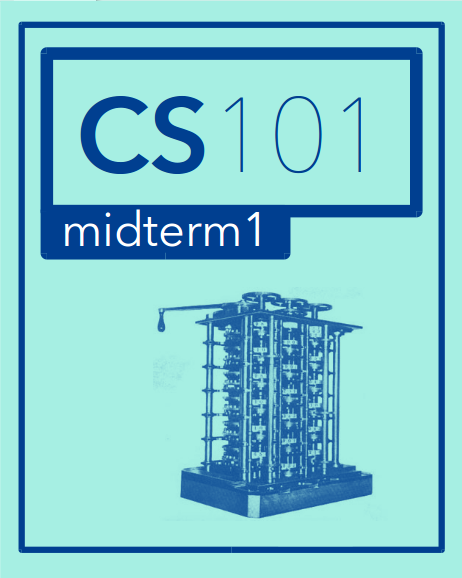
\includegraphics[width=2in]{../img/midterm1-header.png}
\end{center}

\bigskip
\noindent
\begin{itemize}
\item \textbf{Be sure to enter your \underline{NetID} and \underline{the code below} on your Scantron}.
\item Do not turn this page until instructed to do so.
\item There are 30 questions, worth 1 point each.
\item Each question has only \textbf{one} correct answer.
\item You must not communicate with other students during this test.
\item No books, notes, or electronic devices are permitted.
\item This is a 60-minute exam.
\item There are several different versions of this exam.
\end{itemize}

\bigskip\bigskip
\noindent
\textbf{\Large 1. Fill in your information:}

\bigskip
{\Large\bf
\begin{tabular}{ll}
Full Name: & \underbar{\hskip 8cm} \\[0.5em]
UIN (Student Number): & \underbar{\hskip 8cm} \\[0.5em]
NetID: & \underbar{\hskip 8cm}
\end{tabular}
}

\bigskip
\bigskip
\noindent
\textbf{\Large 2. Fill in the following answers on the Scantron form:}

%%%%%%%%%%%%%%%%%%%%%%%%%%%%%%%%%%%%%%%%%%%%%%%%%%%%%%%%%
%%%%%%%%%%%%%%%%%%%%%%%%%%%%%%%%%%%%%%%%%%%%%%%%%%%%%%%%%

\begin{enumerate}
\item[92.] E
\item[93.] A
\item[94.] B
\item[95.] D
\item[96.] E
\end{enumerate}

\newpage

% Zone 1


%%%%%%%%%%%%%%%%%%%%%%%%%%%%%%%%%%%%%%%%%%%%%%%%%%%%%%%%%



\newpage
\noindent
1. (1 point)
\begin{verbatim}
x=str(3)+"str(3)"
\end{verbatim}
What is the \textbf{value} of \texttt{x} after this program is executed?


\begin{enumerate}
\item[(A)] $\bigstar$ 
\begin{verbatim}"3str(3)"\end{verbatim}

\item[(B)]
None of the other answers are correct.

\item[(C)]
\begin{verbatim}"33"\end{verbatim}

\item[(D)]
\begin{verbatim}"333"\end{verbatim}

\item[(E)]
\begin{verbatim}33\end{verbatim}

\end{enumerate}

\vspace*{2em}
\hrule
\vspace{2em}

\noindent {\bf Solution.} 
\vspace{2em}
\hrule height 2pt


\newpage
\noindent
2. (1 point)
Consider the following program:
\begin{verbatim}
a=["merlin","sir agravaine","king pellinore"]
b=[ ]
for i in range(0,4):
    b.append(a[0-i].title())
\end{verbatim}
What is the \textbf{value} of b after this program is executed?


\begin{enumerate}
\item[(A)]
\begin{verbatim}['Merlin', 'Sir Agravaine', 'King Pellinore', 'Merlin']\end{verbatim}

\item[(B)]
\begin{verbatim}[ ]\end{verbatim}

\item[(C)]
\begin{verbatim}['Merlin', 'King Pellinore', 'Sir Agravaine']\end{verbatim}

\item[(D)]
\begin{verbatim}['King Pellinore', 'Sir Agravaine', 'Merlin']\end{verbatim}

\item[(E)] $\bigstar$ 
\begin{verbatim}['Merlin', 'King Pellinore', 'Sir Agravaine', 'Merlin']\end{verbatim}

\end{enumerate}

\vspace*{2em}
\hrule
\vspace{2em}

\noindent {\bf Solution.} 
\vspace{2em}
\hrule height 2pt


\newpage
\noindent
3. (1 point)
Consider the following program:
\begin{verbatim}
s="Hobbes"
i=0
x=-1
while i<len(s):
    if s[i]=='b':
        x=i
    i+=1
\end{verbatim}
What is the \textbf{value} of \texttt{x} after this program is executed?


\begin{enumerate}
\item[(A)]
\begin{verbatim}-1\end{verbatim}

\item[(B)] $\bigstar$ 
\begin{verbatim}3\end{verbatim}

\item[(C)]
\begin{verbatim}5\end{verbatim}

\item[(D)]
\begin{verbatim}2\end{verbatim}

\item[(E)]
\begin{verbatim}4\end{verbatim}

\end{enumerate}

\vspace*{2em}
\hrule
\vspace{2em}

\noindent {\bf Solution.} 
\vspace{2em}
\hrule height 2pt


\newpage
\noindent
4. (1 point)
Consider the following program:
\begin{verbatim}
x=2
a=6
if (a%3)==2:
    x=x**3
elif(a%3)==1:
    x=x**2
else:
    x=x**1
\end{verbatim}
What is the \textbf{value} of \texttt{x} after this program is executed?


\begin{enumerate}
\item[(A)]
\begin{verbatim}8\end{verbatim}

\item[(B)]
None of the other answers are correct.

\item[(C)]
\begin{verbatim}4\end{verbatim}

\item[(D)] $\bigstar$ 
\begin{verbatim}2\end{verbatim}

\item[(E)]
\begin{verbatim}16\end{verbatim}

\end{enumerate}

\vspace*{2em}
\hrule
\vspace{2em}

\noindent {\bf Solution.} 
\vspace{2em}
\hrule height 2pt


\newpage
\noindent
5. (1 point)
Consider the following Python program.
\begin{verbatim}
e=[1,3,5,7,9,11]
d=[0,0,0]
for i in range(0,len(e)):
    d[i%3]+=e[i]
x=d[2]
\end{verbatim}
After it is run, what is the final \textbf{value} of \texttt{x}?


\begin{enumerate}
\item[(A)]
\begin{verbatim}8\end{verbatim}

\item[(B)]
\begin{verbatim}7\end{verbatim}

\item[(C)] $\bigstar$ 
\begin{verbatim}16\end{verbatim}

\item[(D)]
\begin{verbatim}12\end{verbatim}

\item[(E)]
\begin{verbatim}0\end{verbatim}

\end{enumerate}

\vspace*{2em}
\hrule
\vspace{2em}

\noindent {\bf Solution.} 
\vspace{2em}
\hrule height 2pt


\newpage
\noindent
6. (1 point)
Consider the following program.
\begin{verbatim}
s="ABCBA"
x=0
y=len(s)-1
while s[x]==s[y] and x<=y:
    x+=1
    y-=1
\end{verbatim}
After it is run, what is the final \textbf{value} of \texttt{x}?


\begin{enumerate}
\item[(A)] $\bigstar$ 
\begin{verbatim}3\end{verbatim}

\item[(B)]
\begin{verbatim}4\end{verbatim}

\item[(C)]
\begin{verbatim}0\end{verbatim}

\item[(D)]
\begin{verbatim}1\end{verbatim}

\item[(E)]
\begin{verbatim}2\end{verbatim}

\end{enumerate}

\vspace*{2em}
\hrule
\vspace{2em}

\noindent {\bf Solution.} 
\vspace{2em}
\hrule height 2pt


\newpage
\noindent
7. (1 point)
Consider the following program:
\begin{verbatim}
i=3
x=2
while i < 7:
    x+=i
    i+=2
\end{verbatim}
What is the \textbf{value} of \texttt{x} after this program is executed?


\begin{enumerate}
\item[(A)]
\begin{verbatim}11\end{verbatim}

\item[(B)]
\begin{verbatim}13\end{verbatim}

\item[(C)] $\bigstar$ 
\begin{verbatim}10\end{verbatim}

\item[(D)]
\begin{verbatim}12\end{verbatim}

\item[(E)]
\begin{verbatim}14\end{verbatim}

\end{enumerate}

\vspace*{2em}
\hrule
\vspace{2em}

\noindent {\bf Solution.} 
\vspace{2em}
\hrule height 2pt


\newpage
\noindent
8. (1 point)
Consider the following program:
\begin{verbatim}
s="ECTOR"
t="GAWAIN"
x=(len(s)/(len(t)-1))+1
\end{verbatim}
What is the \textbf{type} of \texttt{x} after this program is executed?


\begin{enumerate}
\item[(A)]
\begin{verbatim}None\end{verbatim}

\item[(B)]
\begin{verbatim}String\end{verbatim}

\item[(C)]
\begin{verbatim}Boolean\end{verbatim}

\item[(D)]
\begin{verbatim}Integer\end{verbatim}

\item[(E)] $\bigstar$ 
\begin{verbatim}Float\end{verbatim}

\end{enumerate}

\vspace*{2em}
\hrule
\vspace{2em}

\noindent {\bf Solution.} 
\vspace{2em}
\hrule height 2pt


\newpage
\noindent
9. (1 point)
Evaluate the following expression:
\begin{verbatim}
len("ABCD"[0:3])
\end{verbatim}
What value is produced?


\begin{enumerate}
\item[(A)]
1

\item[(B)]
4

\item[(C)]
2

\item[(D)] $\bigstar$ 
3

\end{enumerate}

\vspace*{2em}
\hrule
\vspace{2em}

\noindent {\bf Solution.} 
\vspace{2em}
\hrule height 2pt


\newpage
\noindent
10. (1 point)
Consider the following program.
\begin{verbatim}
x=[]
for j in range(0,5):
    if (j%4)==0:
        x.append("-")
    if (j%5)==0:
        x.append("*")
\end{verbatim}
After it is run, what is the final \textbf{value} of \texttt{x}?


\begin{enumerate}
\item[(A)]
\begin{verbatim}["-","*","*"]\end{verbatim}

\item[(B)]
None of the other answers are correct.

\item[(C)] $\bigstar$ 
\begin{verbatim}["-","*","-"]\end{verbatim}

\item[(D)]
\begin{verbatim}["-","-","*"]\end{verbatim}

\item[(E)]
\begin{verbatim}["-","*"]\end{verbatim}

\end{enumerate}

\vspace*{2em}
\hrule
\vspace{2em}

\noindent {\bf Solution.} 
\vspace{2em}
\hrule height 2pt


\newpage
\noindent
11. (1 point)
Consider the following program:
\begin{verbatim}
def fix(s):
    a=list(s)
    a.sort()
    return ''.join(a)

x=["one","two","eleven","twelve"]
s1=fix(x[0]+x[-1])
s2=fix(x[1]+x[-2])

if s1<s2:
    x.sort()
elif s1>s2:
    x.reverse()
else:
    x.append("six")
\end{verbatim}
What is the \textbf{value} of \texttt{x} after this program is executed?


\begin{enumerate}
\item[(A)]
\begin{verbatim}['one', 'two', 'eleven', 'twelve']\end{verbatim}

\item[(B)]
\begin{verbatim}['eleven', 'one', 'twelve', 'two']\end{verbatim}

\item[(C)] $\bigstar$ 
\begin{verbatim}['one', 'two', 'eleven', 'twelve', 'six']\end{verbatim}

\item[(D)]
\begin{verbatim}['twelve', 'eleven', 'two', 'one']\end{verbatim}

\item[(E)]
\begin{verbatim}['two', 'twelve', 'one', 'eleven', 'six']\end{verbatim}

\end{enumerate}

\vspace*{2em}
\hrule
\vspace{2em}

\noindent {\bf Solution.} 
\vspace{2em}
\hrule height 2pt


\newpage
\noindent
12. (1 point)
Consider the following program.
\begin{verbatim}
x=0
i=1
while(i*i)<=9:
    x=x+(i*i)
    i=i+1
\end{verbatim}
After it is run, what is the final \textbf{value} of \texttt{x}?


\begin{enumerate}
\item[(A)] $\bigstar$ 
\begin{verbatim}14\end{verbatim}

\item[(B)]
\begin{verbatim}3\end{verbatim}

\item[(C)]
\begin{verbatim}5\end{verbatim}

\item[(D)]
\begin{verbatim}30\end{verbatim}

\item[(E)]
\begin{verbatim}4\end{verbatim}

\end{enumerate}

\vspace*{2em}
\hrule
\vspace{2em}

\noindent {\bf Solution.} 
\vspace{2em}
\hrule height 2pt


\newpage
\noindent
13. (1 point)
Consider the following program:
\begin{verbatim}
s="-B-O-R-S-"
x=s.split("-")[2:-2]
\end{verbatim}
What is the \textbf{value} of \texttt{x} after this program is executed?


\begin{enumerate}
\item[(A)]
\begin{verbatim}'ORS'\end{verbatim}

\item[(B)]
\begin{verbatim}''\end{verbatim}

\item[(C)] $\bigstar$ 
\begin{verbatim}['O', 'R']\end{verbatim}

\item[(D)]
\begin{verbatim}False\end{verbatim}

\item[(E)]
\begin{verbatim}None\end{verbatim}

\end{enumerate}

\vspace*{2em}
\hrule
\vspace{2em}

\noindent {\bf Solution.} 
\vspace{2em}
\hrule height 2pt


\newpage
\noindent
14. (1 point)
Consider the following incomplete program.
\begin{verbatim}
sum=0
for i in range(0,100):
    ???

\end{verbatim}
The program is intended to sum all of the integers between 1 and 100 (inclusive). What should replace the three question marks to complete the program?


\begin{enumerate}
\item[(A)]
\begin{verbatim}sum+1=sum \end{verbatim}

\item[(B)]
\begin{verbatim}sum=sum+1\end{verbatim}

\item[(C)]
\begin{verbatim}sum=sum+i \end{verbatim}

\item[(D)] $\bigstar$ 
\begin{verbatim}sum=sum+i+1 \end{verbatim}

\end{enumerate}

\vspace*{2em}
\hrule
\vspace{2em}

\noindent {\bf Solution.} 
\vspace{2em}
\hrule height 2pt


\newpage
\noindent
15. (1 point)
Consider the following program:
\begin{verbatim}
a=3
b=4
if a==3:
    a=b
elif a==4:
    a=5
else:
    b=a
\end{verbatim}
What is the \textbf{value} of a after this program is executed?


\begin{enumerate}
\item[(A)] $\bigstar$ 
\begin{verbatim}4\end{verbatim}

\item[(B)]
None of the other answers are correct.

\item[(C)]
\begin{verbatim}5\end{verbatim}

\item[(D)]
\begin{verbatim}3\end{verbatim}

\item[(E)]
\begin{verbatim}7\end{verbatim}

\end{enumerate}

\vspace*{2em}
\hrule
\vspace{2em}

\noindent {\bf Solution.} 
\vspace{2em}
\hrule height 2pt


\newpage
\noindent
16. (1 point)
Consider the following program:
\begin{verbatim}
a=["A","C","C","I","O"]
a.sort()
a[0]=a[-1]
x=""
for e in a:
    x=x+e
\end{verbatim}
What is the \textbf{value} of \texttt{x} after this program is executed?


\begin{enumerate}
\item[(A)]
\begin{verbatim}"ICCOI"\end{verbatim}

\item[(B)]
\begin{verbatim}"ACCIA"\end{verbatim}

\item[(C)] $\bigstar$ 
\begin{verbatim}"OCCIO"\end{verbatim}

\item[(D)]
None of the other answers are correct.

\item[(E)]
\begin{verbatim}"ACCOA"\end{verbatim}

\end{enumerate}

\vspace*{2em}
\hrule
\vspace{2em}

\noindent {\bf Solution.} 
\vspace{2em}
\hrule height 2pt


\newpage
\noindent
17. (1 point)
How can the following mathematical equation be implemented as a Python expression? Assume \verb|a|, \verb|b|, and \verb|sin| have already been defined.
$$a \sin(a^b - b)$$


\begin{enumerate}
\item[(A)]
\begin{verbatim}a*sin(a^b - b)\end{verbatim}

\item[(B)] $\bigstar$ 
\begin{verbatim}a*sin(a**b - b)\end{verbatim}

\item[(C)]
\begin{verbatim}a*sin(b^a - b)\end{verbatim}

\item[(D)]
\begin{verbatim}a sin(a**b - b)\end{verbatim}

\item[(E)]
None of the other answers are correct.

\end{enumerate}

\vspace*{2em}
\hrule
\vspace{2em}

\noindent {\bf Solution.} 
\vspace{2em}
\hrule height 2pt


\newpage
\noindent
18. (1 point)
Consider the following program.
\begin{verbatim}
kay = 2
wart = 3

def knight(kay,wart):
    wart += 2
    kay += 3
    return wart + kay

kay = knight(wart, kay) + knight(kay, wart)
\end{verbatim}
After it is run, what is the final \textbf{value} of \texttt{kay}?


\begin{enumerate}
\item[(A)] $\bigstar$ 
None of the other answers are correct.

\item[(B)]
\begin{verbatim}5\end{verbatim}

\item[(C)]
\begin{verbatim}2\end{verbatim}

\item[(D)]
\begin{verbatim}3\end{verbatim}

\end{enumerate}

\vspace*{2em}
\hrule
\vspace{2em}

\noindent {\bf Solution.} 
\vspace{2em}
\hrule height 2pt


\newpage
\noindent
19. (1 point)
Consider the following program:
\begin{verbatim}
pi="3.14159"
e="2.71828"
x=pi*len(e)+pi
\end{verbatim}
What is the \textbf{type} of \texttt{x} after this program is executed?


\begin{enumerate}
\item[(A)]
\begin{verbatim}Integer\end{verbatim}

\item[(B)]
\begin{verbatim}None\end{verbatim}

\item[(C)]
\begin{verbatim}Float\end{verbatim}

\item[(D)]
\begin{verbatim}Boolean\end{verbatim}

\item[(E)] $\bigstar$ 
\begin{verbatim}String\end{verbatim}

\end{enumerate}

\vspace*{2em}
\hrule
\vspace{2em}

\noindent {\bf Solution.} 
\vspace{2em}
\hrule height 2pt


\newpage
\noindent
20. (1 point)
Evaluate the following expression:
\begin{verbatim}
[1,2]*len("3")
\end{verbatim}
What value is produced?


\begin{enumerate}
\item[(A)]
\begin{verbatim}[1,2,3]\end{verbatim}

\item[(B)]
\begin{verbatim}[1,2,1]\end{verbatim}

\item[(C)]
\begin{verbatim}[1,2,1,2,1,2]\end{verbatim}

\item[(D)] $\bigstar$ 
\begin{verbatim}[1,2]\end{verbatim}

\end{enumerate}

\vspace*{2em}
\hrule
\vspace{2em}

\noindent {\bf Solution.} 
\vspace{2em}
\hrule height 2pt


\newpage
\noindent
21. (1 point)
For this problem, you should compose a function which accomplishes a given task using the available code blocks arranged in the correct functional order.  \emph{We ignore indentation for this problem.}

\texttt{find\_max} should accept a \texttt{list} and return the value of the maximum item in the \texttt{list}.  (\texttt{None} is always the lowest value in any numeric comparison, so you may use it as an initializer.)

\begin{verbatim}
def find_max(my_list):
\end{verbatim}

\begin{enumerate}[1]
\item \texttt{max\_val = i}
\item \texttt{max\_val = None}
\item \texttt{for i in range(len(my\_list)):}
\item \texttt{if i > max\_val:}
\item \texttt{max\_val = my\_list[i]}
\item \texttt{return max\_val}
\item \texttt{for i in range(my\_list):}
\item \texttt{if my\_list[i] > max\_val:}
\item \texttt{print(max\_val)}
\end{enumerate}



\begin{enumerate}
\item[(A)] $\bigstar$ 
2, 3, 8, 5, 6

\item[(B)]
2, 7, 4, 5, 6

\item[(C)]
3, 2, 8, 5, 9

\item[(D)]
2, 3, 8, 1, 6

\item[(E)]
2, 3, 4, 1, 6

\end{enumerate}

\vspace*{2em}
\hrule
\vspace{2em}

\noindent {\bf Solution.} 
\vspace{2em}
\hrule height 2pt


\newpage
\noindent
22. (1 point)
What is the result of the following expression?
\begin{verbatim}
[ 1, 2, 3 ] * 3
\end{verbatim}


\begin{enumerate}
\item[(A)]
\begin{verbatim}[3.0, 6.0, 9.0]\end{verbatim}

\item[(B)]
\begin{verbatim}(3, 6, 9)\end{verbatim}

\item[(C)]
\begin{verbatim}[3, 6, 9]\end{verbatim}

\item[(D)]
\begin{verbatim}[1.0, 2.0, 3.0, 1.0, 2.0, 3.0, 1.0, 2.0, 3.0]\end{verbatim}

\item[(E)] $\bigstar$ 
\begin{verbatim}[1, 2, 3, 1, 2, 3, 1, 2, 3]\end{verbatim}

\end{enumerate}

\vspace*{2em}
\hrule
\vspace{2em}

\noindent {\bf Solution.} 
\vspace{2em}
\hrule height 2pt


\newpage
\noindent
23. (1 point)
Consider the following program:
\begin{verbatim}
x=0
for i in range(2,8):
    if i%3==0:
        x+=3
    elif i%2==0:
        x+=2
    else:
        x+=1
\end{verbatim}
What is the \textbf{value} of \texttt{x} after this program is executed?


\begin{enumerate}
\item[(A)] $\bigstar$ 
\begin{verbatim}12\end{verbatim}

\item[(B)]
\begin{verbatim}13\end{verbatim}

\item[(C)]
\begin{verbatim}10\end{verbatim}

\item[(D)]
\begin{verbatim}11\end{verbatim}

\item[(E)]
\begin{verbatim}14\end{verbatim}

\end{enumerate}

\vspace*{2em}
\hrule
\vspace{2em}

\noindent {\bf Solution.} 
\vspace{2em}
\hrule height 2pt


\newpage
\noindent
24. (1 point)
Consider the following program:
\begin{verbatim}
x=[1,2,3,4,5,6,7,8,9]
x=x[2:-2]
i=1
while i < 3:
    x[i]+=1
    i+=1
\end{verbatim}
What is the \textbf{value} of \texttt{x} after this program is executed?


\begin{enumerate}
\item[(A)]
\begin{verbatim}[3, 5, 6, 6]\end{verbatim}

\item[(B)]
\begin{verbatim}[2, 4, 5, 5, 6, 7]\end{verbatim}

\item[(C)] $\bigstar$ 
\begin{verbatim}[3, 5, 6, 6, 7]\end{verbatim}

\item[(D)]
\begin{verbatim}[2, 4, 5, 6, 6, 7]\end{verbatim}

\item[(E)]
\begin{verbatim}[3, 5, 6, 6, 7, 8]\end{verbatim}

\end{enumerate}

\vspace*{2em}
\hrule
\vspace{2em}

\noindent {\bf Solution.} 
\vspace{2em}
\hrule height 2pt


\newpage
\noindent
25. (1 point)
Consider the following program:
\begin{verbatim}
x=[1,2,3]
def f(a):
    s=""
    a.reverse()
    for i in a:
        s+=str(i)
    return s

x.append(f(x))
\end{verbatim}
What is the \textbf{value} of \texttt{x} after this program is executed?


\begin{enumerate}
\item[(A)]
\begin{verbatim}[1, 2, 3, '321']\end{verbatim}

\item[(B)] $\bigstar$ 
\begin{verbatim}[3, 2, 1, '321']\end{verbatim}

\item[(C)]
\begin{verbatim}[3, 2, 1]\end{verbatim}

\item[(D)]
\begin{verbatim}[1, 2, 3, 6]\end{verbatim}

\item[(E)]
\begin{verbatim}[1, 2, 3]\end{verbatim}

\end{enumerate}

\vspace*{2em}
\hrule
\vspace{2em}

\noindent {\bf Solution.} 
\vspace{2em}
\hrule height 2pt


\newpage
\noindent
26. (1 point)
Consider the following program.
\begin{verbatim}
def artificing(s):
    return s+"%i" % 2
    return s*2
    return s

s=artificing("MERLIN")
\end{verbatim}
After it is run, what is the final \textbf{value} of s?


\begin{enumerate}
\item[(A)] $\bigstar$ 
\begin{verbatim}"MERLIN2"\end{verbatim}

\item[(B)]
\begin{verbatim}None\end{verbatim}

\item[(C)]
\begin{verbatim}"MERLIN%i"\end{verbatim}

\item[(D)]
\begin{verbatim}0\end{verbatim}

\item[(E)]
\begin{verbatim}"MERLINMERLIN"\end{verbatim}

\end{enumerate}

\vspace*{2em}
\hrule
\vspace{2em}

\noindent {\bf Solution.} 
\vspace{2em}
\hrule height 2pt


\newpage
\noindent
27. (1 point)
Consider the following incomplete function.
\begin{verbatim}
def isdivisible(m,n):
    if ???:
        return False
    else:
        return True
\end{verbatim}
The function is intended to return True if the input parameter m is evenly divisible by the parameter n and False otherwise. For example, \verb|isdivisible(4,2)| should return \verb|True|, but \verb|isdivisible(5,3)| should return \verb|False|. What should replace the three question marks to complete the function?


\begin{enumerate}
\item[(A)]
\begin{verbatim}(n % m) == 0 \end{verbatim}

\item[(B)]
\begin{verbatim}(m // n) != 0 \end{verbatim}

\item[(C)] $\bigstar$ 
\begin{verbatim}(m % n) != 0 \end{verbatim}

\item[(D)]
\begin{verbatim}(n // m) == 0 \end{verbatim}

\end{enumerate}

\vspace*{2em}
\hrule
\vspace{2em}

\noindent {\bf Solution.} 
\vspace{2em}
\hrule height 2pt


\newpage
\noindent
28. (1 point)
Consider the following incomplete Python program.
\begin{verbatim}
s="".join(["0","1","2","1"])
x=0
for i in range(len(s)-1):
    x+=int(???)
\end{verbatim}
What should replace the three question marks so the resulting value of \texttt{x} is 34?


\begin{enumerate}
\item[(A)] $\bigstar$ 
\begin{verbatim}s[i:i+2]\end{verbatim}

\item[(B)]
\begin{verbatim}s[i:i-1]\end{verbatim}

\item[(C)]
\begin{verbatim}s[i+1:i+2]\end{verbatim}

\item[(D)]
\begin{verbatim}s[i:i+1]\end{verbatim}

\end{enumerate}

\vspace*{2em}
\hrule
\vspace{2em}

\noindent {\bf Solution.} 
\vspace{2em}
\hrule height 2pt


\newpage
\noindent
29. (1 point)
Consider the following program:
\begin{verbatim}
x="KING ARTHUR-MORGANA LEFAY-SIR BEDIVERE".split("-")
y=x
y.reverse()
\end{verbatim}
What is the \textbf{value} of \texttt{x} after this program is executed?


\begin{enumerate}
\item[(A)]
\begin{verbatim}['KING ARTHUR', 'MORGANA LEFAY', 'SIR BEDIVERE']\end{verbatim}

\item[(B)] $\bigstar$ 
\begin{verbatim}['SIR BEDIVERE', 'MORGANA LEFAY', 'KING ARTHUR']\end{verbatim}

\item[(C)]
\begin{verbatim}['BEDIVERE', 'LEFAY-SIR', 'ARTHUR-MORGANA', 'KING']\end{verbatim}

\item[(D)]
\begin{verbatim}None\end{verbatim}

\item[(E)]
\begin{verbatim}['KING', 'ARTHUR-MORGANA', 'LEFAY-SIR', 'BEDIVERE']\end{verbatim}

\end{enumerate}

\vspace*{2em}
\hrule
\vspace{2em}

\noindent {\bf Solution.} 
\vspace{2em}
\hrule height 2pt


\newpage
\noindent
30. (1 point)
Consider the following program:
\begin{verbatim}
s="TRIS %i"
t="ISEU"
x=s % len(t)
\end{verbatim}
What is the \textbf{type} of \texttt{x} after this program is executed?


\begin{enumerate}
\item[(A)]
\begin{verbatim}Float\end{verbatim}

\item[(B)]
\begin{verbatim}Boolean\end{verbatim}

\item[(C)]
\begin{verbatim}Integer\end{verbatim}

\item[(D)]
\begin{verbatim}None\end{verbatim}

\item[(E)] $\bigstar$ 
\begin{verbatim}String\end{verbatim}

\end{enumerate}

\vspace*{2em}
\hrule
\vspace{2em}

\noindent {\bf Solution.} 
\vspace{2em}
\hrule height 2pt

%%%%%%%%%%%%%%%%%%%%%%%%%%%%%%%%%%%%%%%%%%%%%%%%%%%%%%%%%%%%%%%%%%%%%%
%%%%%%%%%%%%%%%%%%%%%%%%%%%%%%%%%%%%%%%%%%%%%%%%%%%%%%%%%%%%%%%%%%%%%%
%%%%%%%%%%%%%%%%%%%%%%%%%%%%%%%%%%%%%%%%%%%%%%%%%%%%%%%%%%%%%%%%%%%%%%
%%%%%%%%%%%%%%%%%%%%%%%%%%%%%%%%%%%%%%%%%%%%%%%%%%%%%%%%%%%%%%%%%%%%%%
% Exam number 31

\message{Exam 31/50}
\cleardoublepage
\setcounter{page}{1}


\begin{center}
%\textbf{\Large CS 101 Midterm \#1}
%
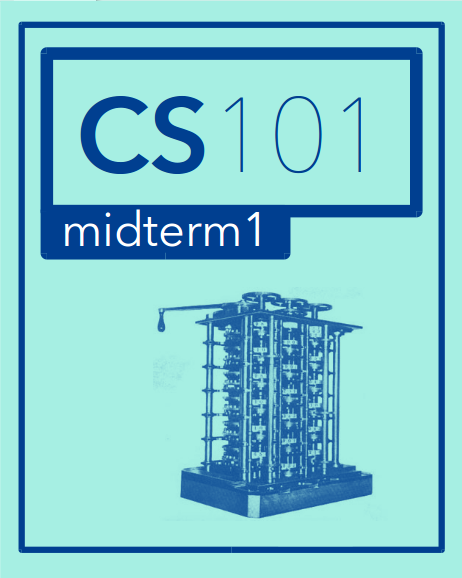
\includegraphics[width=2in]{../img/midterm1-header.png}
\end{center}

\bigskip
\noindent
\begin{itemize}
\item \textbf{Be sure to enter your \underline{NetID} and \underline{the code below} on your Scantron}.
\item Do not turn this page until instructed to do so.
\item There are 30 questions, worth 1 point each.
\item Each question has only \textbf{one} correct answer.
\item You must not communicate with other students during this test.
\item No books, notes, or electronic devices are permitted.
\item This is a 60-minute exam.
\item There are several different versions of this exam.
\end{itemize}

\bigskip\bigskip
\noindent
\textbf{\Large 1. Fill in your information:}

\bigskip
{\Large\bf
\begin{tabular}{ll}
Full Name: & \underbar{\hskip 8cm} \\[0.5em]
UIN (Student Number): & \underbar{\hskip 8cm} \\[0.5em]
NetID: & \underbar{\hskip 8cm}
\end{tabular}
}

\bigskip
\bigskip
\noindent
\textbf{\Large 2. Fill in the following answers on the Scantron form:}

%%%%%%%%%%%%%%%%%%%%%%%%%%%%%%%%%%%%%%%%%%%%%%%%%%%%%%%%%
%%%%%%%%%%%%%%%%%%%%%%%%%%%%%%%%%%%%%%%%%%%%%%%%%%%%%%%%%

\begin{enumerate}
\item[92.] A
\item[93.] B
\item[94.] B
\item[95.] A
\item[96.] C
\end{enumerate}

\newpage

% Zone 1


%%%%%%%%%%%%%%%%%%%%%%%%%%%%%%%%%%%%%%%%%%%%%%%%%%%%%%%%%



\newpage
\noindent
1. (1 point)
Consider the following program.
\begin{verbatim}
def artificing(s):
    return s*2
    return s+"%i" % 2
    return s

s=artificing("MERLIN")
\end{verbatim}
After it is run, what is the final \textbf{value} of s?


\begin{enumerate}
\item[(A)]
\begin{verbatim}None\end{verbatim}

\item[(B)] $\bigstar$ 
\begin{verbatim}"MERLINMERLIN"\end{verbatim}

\item[(C)]
\begin{verbatim}12\end{verbatim}

\item[(D)]
\begin{verbatim}"MERLIN2"\end{verbatim}

\item[(E)]
\begin{verbatim}"MERLIN"\end{verbatim}

\end{enumerate}

\vspace*{2em}
\hrule
\vspace{2em}

\noindent {\bf Solution.} 
\vspace{2em}
\hrule height 2pt


\newpage
\noindent
2. (1 point)
Consider the following program:
\begin{verbatim}
s="-B-O-R-S-"
x=s.split("-")[2:-2]
\end{verbatim}
What is the \textbf{value} of \texttt{x} after this program is executed?


\begin{enumerate}
\item[(A)]
\begin{verbatim}''\end{verbatim}

\item[(B)]
\begin{verbatim}'ORS'\end{verbatim}

\item[(C)]
\begin{verbatim}False\end{verbatim}

\item[(D)]
\begin{verbatim}None\end{verbatim}

\item[(E)] $\bigstar$ 
\begin{verbatim}['O', 'R']\end{verbatim}

\end{enumerate}

\vspace*{2em}
\hrule
\vspace{2em}

\noindent {\bf Solution.} 
\vspace{2em}
\hrule height 2pt


\newpage
\noindent
3. (1 point)
Consider the following incomplete function.
\begin{verbatim}
def ismultiple(m,n):
    if ???:
        return False
    else:
        return True
\end{verbatim}
The function is intended to return True if the input parameter m is a multiple of parameter n and False otherwise. For example, \verb|ismultiple(4,2)| should return \verb|True|, but \verb|ismultiple(5,3)| should return \verb|False|. What should replace the three question marks to complete the function?


\begin{enumerate}
\item[(A)]
\begin{verbatim}(n // m) == 0 \end{verbatim}

\item[(B)] $\bigstar$ 
\begin{verbatim}(m % n) != 0 \end{verbatim}

\item[(C)]
\begin{verbatim}(n % m) == 0 \end{verbatim}

\item[(D)]
\begin{verbatim}(m // n) != 0 \end{verbatim}

\end{enumerate}

\vspace*{2em}
\hrule
\vspace{2em}

\noindent {\bf Solution.} 
\vspace{2em}
\hrule height 2pt


\newpage
\noindent
4. (1 point)
Consider the following program:
\begin{verbatim}
x=2
a=6
if (a%3)==2:
    x=x**3
elif(a%3)==1:
    x=x**2
else:
    x=x**1
\end{verbatim}
What is the \textbf{value} of \texttt{x} after this program is executed?


\begin{enumerate}
\item[(A)]
None of the other answers are correct.

\item[(B)]
\begin{verbatim}4\end{verbatim}

\item[(C)] $\bigstar$ 
\begin{verbatim}2\end{verbatim}

\item[(D)]
\begin{verbatim}16\end{verbatim}

\item[(E)]
\begin{verbatim}8\end{verbatim}

\end{enumerate}

\vspace*{2em}
\hrule
\vspace{2em}

\noindent {\bf Solution.} 
\vspace{2em}
\hrule height 2pt


\newpage
\noindent
5. (1 point)
How can the following mathematical equation be implemented as a Python expression? Assume \verb|a|, \verb|b|, and \verb|cos| have already been defined.
$$a^b \cos(a - b)$$


\begin{enumerate}
\item[(A)]
None of the other answers are correct.

\item[(B)]
\begin{verbatim}(a**b)cos(a-b)\end{verbatim}

\item[(C)]
\begin{verbatim}(b^a)cos(a-b)\end{verbatim}

\item[(D)] $\bigstar$ 
\begin{verbatim}(a**b)*cos(a-b)\end{verbatim}

\item[(E)]
\begin{verbatim}(a^b)*cos(a-b)\end{verbatim}

\end{enumerate}

\vspace*{2em}
\hrule
\vspace{2em}

\noindent {\bf Solution.} 
\vspace{2em}
\hrule height 2pt


\newpage
\noindent
6. (1 point)
Consider the following program:
\begin{verbatim}
s="TRIS %i"
t="ISEU"
x=s % len(t)
\end{verbatim}
What is the \textbf{type} of \texttt{x} after this program is executed?


\begin{enumerate}
\item[(A)]
\begin{verbatim}None\end{verbatim}

\item[(B)]
\begin{verbatim}Integer\end{verbatim}

\item[(C)]
\begin{verbatim}Float\end{verbatim}

\item[(D)] $\bigstar$ 
\begin{verbatim}String\end{verbatim}

\item[(E)]
\begin{verbatim}Boolean\end{verbatim}

\end{enumerate}

\vspace*{2em}
\hrule
\vspace{2em}

\noindent {\bf Solution.} 
\vspace{2em}
\hrule height 2pt


\newpage
\noindent
7. (1 point)
Evaluate the following expression:
\begin{verbatim}
[1,2]*len("3")
\end{verbatim}
What value is produced?


\begin{enumerate}
\item[(A)]
\begin{verbatim}[1,2,1]\end{verbatim}

\item[(B)]
\begin{verbatim}[1,2,3]\end{verbatim}

\item[(C)] $\bigstar$ 
\begin{verbatim}[1,2]\end{verbatim}

\item[(D)]
\begin{verbatim}[1,2,1,2,1,2]\end{verbatim}

\end{enumerate}

\vspace*{2em}
\hrule
\vspace{2em}

\noindent {\bf Solution.} 
\vspace{2em}
\hrule height 2pt


\newpage
\noindent
8. (1 point)
Consider the following incomplete program.
\begin{verbatim}
sum=0
???:
    sum=sum+i

\end{verbatim}
The program is intended to sum all of the integers between 1 and 100 (inclusive). What should replace the three question marks to complete the program?


\begin{enumerate}
\item[(A)]
\begin{verbatim}for i in range(0,100)\end{verbatim}

\item[(B)]
\begin{verbatim}while i in range(100)\end{verbatim}

\item[(C)] $\bigstar$ 
\begin{verbatim}for i in range(1,101) \end{verbatim}

\item[(D)]
\begin{verbatim}while i<=100 \end{verbatim}

\end{enumerate}

\vspace*{2em}
\hrule
\vspace{2em}

\noindent {\bf Solution.} 
\vspace{2em}
\hrule height 2pt


\newpage
\noindent
9. (1 point)
Consider the following program:
\begin{verbatim}
i=3
x=2
while i < 7:
    x+=i
    i+=2
\end{verbatim}
What is the \textbf{value} of \texttt{x} after this program is executed?


\begin{enumerate}
\item[(A)]
\begin{verbatim}12\end{verbatim}

\item[(B)]
\begin{verbatim}14\end{verbatim}

\item[(C)] $\bigstar$ 
\begin{verbatim}10\end{verbatim}

\item[(D)]
\begin{verbatim}11\end{verbatim}

\item[(E)]
\begin{verbatim}13\end{verbatim}

\end{enumerate}

\vspace*{2em}
\hrule
\vspace{2em}

\noindent {\bf Solution.} 
\vspace{2em}
\hrule height 2pt


\newpage
\noindent
10. (1 point)
Consider the following program:
\begin{verbatim}
def fix(s):
    a=list(s)
    a.sort()
    return ''.join(a)

x=["one","two","eleven","twelve"]
s1=fix(x[0]+x[-1])
s2=fix(x[1]+x[-2])

if s1==s2:
    x.sort()
elif s1<s2:
    x.reverse()
else:
    x.append("six")
\end{verbatim}
What is the \textbf{value} of \texttt{x} after this program is executed?


\begin{enumerate}
\item[(A)]
\begin{verbatim}['one', 'two', 'eleven', 'twelve', 'six']\end{verbatim}

\item[(B)]
\begin{verbatim}['one', 'two', 'eleven', 'twelve']\end{verbatim}

\item[(C)]
\begin{verbatim}['twelve', 'eleven', 'two', 'one']\end{verbatim}

\item[(D)] $\bigstar$ 
\begin{verbatim}['eleven', 'one', 'twelve', 'two']\end{verbatim}

\item[(E)]
\begin{verbatim}['two', 'twelve', 'one', 'eleven', 'six']\end{verbatim}

\end{enumerate}

\vspace*{2em}
\hrule
\vspace{2em}

\noindent {\bf Solution.} 
\vspace{2em}
\hrule height 2pt


\newpage
\noindent
11. (1 point)
Consider the following program:
\begin{verbatim}
x="KING ARTHUR-MORGANA LEFAY-SIR BEDIVERE".split("-")
y=x
x=y.reverse()
\end{verbatim}
What is the \textbf{value} of \texttt{x} after this program is executed?


\begin{enumerate}
\item[(A)]
\begin{verbatim}['SIR BEDIVERE', 'MORGANA LEFAY', 'KING ARTHUR']\end{verbatim}

\item[(B)]
\begin{verbatim}['KING ARTHUR', 'MORGANA LEFAY', 'SIR BEDIVERE']\end{verbatim}

\item[(C)]
\begin{verbatim}['KING', 'ARTHUR-MORGANA', 'LEFAY-SIR', 'BEDIVERE']\end{verbatim}

\item[(D)]
\begin{verbatim}['BEDIVERE', 'LEFAY-SIR', 'ARTHUR-MORGANA', 'KING']\end{verbatim}

\item[(E)] $\bigstar$ 
\begin{verbatim}None\end{verbatim}

\end{enumerate}

\vspace*{2em}
\hrule
\vspace{2em}

\noindent {\bf Solution.} 
\vspace{2em}
\hrule height 2pt


\newpage
\noindent
12. (1 point)
Evaluate the following expression:
\begin{verbatim}
len("ABCDE"[1:4])
\end{verbatim}
What value is produced?


\begin{enumerate}
\item[(A)]
1

\item[(B)]
5

\item[(C)]
4

\item[(D)] $\bigstar$ 
3

\end{enumerate}

\vspace*{2em}
\hrule
\vspace{2em}

\noindent {\bf Solution.} 
\vspace{2em}
\hrule height 2pt


\newpage
\noindent
13. (1 point)
Consider the following Python program.
\begin{verbatim}
e=[1,3,5,7,9,11]
d=[0,0,0]
for i in range(0,len(e)):
    d[i%3]+=e[i]
x=d[1]
\end{verbatim}
After it is run, what is the final \textbf{value} of \texttt{x}?


\begin{enumerate}
\item[(A)]
\begin{verbatim}3\end{verbatim}

\item[(B)] $\bigstar$ 
\begin{verbatim}12\end{verbatim}

\item[(C)]
\begin{verbatim}8\end{verbatim}

\item[(D)]
\begin{verbatim}16\end{verbatim}

\item[(E)]
\begin{verbatim}0\end{verbatim}

\end{enumerate}

\vspace*{2em}
\hrule
\vspace{2em}

\noindent {\bf Solution.} 
\vspace{2em}
\hrule height 2pt


\newpage
\noindent
14. (1 point)
Consider the following program:
\begin{verbatim}
a=["merlin","sir agravaine","king pellinore"]
b=[ ]
for i in range(0,4):
    b.append(a[0-i].title())
\end{verbatim}
What is the \textbf{value} of b after this program is executed?


\begin{enumerate}
\item[(A)]
\begin{verbatim}['King Pellinore', 'Sir Agravaine', 'Merlin']\end{verbatim}

\item[(B)] $\bigstar$ 
\begin{verbatim}['Merlin', 'King Pellinore', 'Sir Agravaine', 'Merlin']\end{verbatim}

\item[(C)]
\begin{verbatim}['Merlin', 'King Pellinore', 'Sir Agravaine']\end{verbatim}

\item[(D)]
\begin{verbatim}['Merlin', 'Sir Agravaine', 'King Pellinore', 'Merlin']\end{verbatim}

\item[(E)]
\begin{verbatim}[ ]\end{verbatim}

\end{enumerate}

\vspace*{2em}
\hrule
\vspace{2em}

\noindent {\bf Solution.} 
\vspace{2em}
\hrule height 2pt


\newpage
\noindent
15. (1 point)
Consider the following program:
\begin{verbatim}
x=[1,2,3]
def f(a):
    s=""
    a.append(4)
    for i in a:
        s+=str(i)
    return s

x.append(f(x))
\end{verbatim}
What is the \textbf{value} of \texttt{x} after this program is executed?


\begin{enumerate}
\item[(A)]
\begin{verbatim}[1, 2, 3, '1234']\end{verbatim}

\item[(B)]
\begin{verbatim}[1, 2, 3, 10]\end{verbatim}

\item[(C)] $\bigstar$ 
\begin{verbatim}[1, 2, 3, 4, '1234']\end{verbatim}

\item[(D)]
\begin{verbatim}[1, 2, 3, '123']\end{verbatim}

\item[(E)]
\begin{verbatim}[1, 2, 3]\end{verbatim}

\end{enumerate}

\vspace*{2em}
\hrule
\vspace{2em}

\noindent {\bf Solution.} 
\vspace{2em}
\hrule height 2pt


\newpage
\noindent
16. (1 point)
Consider the following program:
\begin{verbatim}
x=[1,2,3,4,5,6,7,8,9]
x=x[2:-2]
i=1
while i < 3:
    x[i]+=1
    i+=1
\end{verbatim}
What is the \textbf{value} of \texttt{x} after this program is executed?


\begin{enumerate}
\item[(A)]
\begin{verbatim}[2, 4, 5, 6, 6, 7]\end{verbatim}

\item[(B)]
\begin{verbatim}[2, 4, 5, 5, 6, 7]\end{verbatim}

\item[(C)] $\bigstar$ 
\begin{verbatim}[3, 5, 6, 6, 7]\end{verbatim}

\item[(D)]
\begin{verbatim}[3, 5, 6, 6]\end{verbatim}

\item[(E)]
\begin{verbatim}[3, 5, 6, 6, 7, 8]\end{verbatim}

\end{enumerate}

\vspace*{2em}
\hrule
\vspace{2em}

\noindent {\bf Solution.} 
\vspace{2em}
\hrule height 2pt


\newpage
\noindent
17. (1 point)
Consider the following program.
\begin{verbatim}
s="BBCAA"
x=0
y=len(s)-1
while s[x]!=s[y] and x<len(s):
    x+=1
    y-=1
\end{verbatim}
After it is run, what is the final \textbf{value} of \texttt{x}?


\begin{enumerate}
\item[(A)]
\begin{verbatim}3\end{verbatim}

\item[(B)]
\begin{verbatim}0\end{verbatim}

\item[(C)]
\begin{verbatim}1\end{verbatim}

\item[(D)] $\bigstar$ 
\begin{verbatim}2\end{verbatim}

\item[(E)]
\begin{verbatim}4\end{verbatim}

\end{enumerate}

\vspace*{2em}
\hrule
\vspace{2em}

\noindent {\bf Solution.} 
\vspace{2em}
\hrule height 2pt


\newpage
\noindent
18. (1 point)
For this problem, you should compose a function which accomplishes a given task using the available code blocks arranged in the correct functional order.  \emph{We ignore indentation for this problem.}

\texttt{find\_max} should accept a \texttt{list} and return the value of the maximum item in the \texttt{list}.  (\texttt{None} is always the lowest value in any numeric comparison, so you may use it as an initializer.)

\begin{verbatim}
def find_max(my_list):
\end{verbatim}

\begin{enumerate}[1]
\item \texttt{max\_val = i}
\item \texttt{max\_val = None}
\item \texttt{for i in range(len(my\_list)):}
\item \texttt{if i > max\_val:}
\item \texttt{max\_val = my\_list[i]}
\item \texttt{return max\_val}
\item \texttt{for i in range(my\_list):}
\item \texttt{if my\_list[i] > max\_val:}
\item \texttt{print(max\_val)}
\end{enumerate}



\begin{enumerate}
\item[(A)]
2, 3, 4, 1, 6

\item[(B)]
2, 7, 4, 5, 6

\item[(C)] $\bigstar$ 
2, 3, 8, 5, 6

\item[(D)]
2, 3, 8, 1, 6

\item[(E)]
3, 2, 8, 5, 9

\end{enumerate}

\vspace*{2em}
\hrule
\vspace{2em}

\noindent {\bf Solution.} 
\vspace{2em}
\hrule height 2pt


\newpage
\noindent
19. (1 point)
Consider the following program:
\begin{verbatim}
a=3
b=4
if a!=b:
    a=b
elif a==4:
    a=5
else:
    b=a
\end{verbatim}
What is the \textbf{value} of a after this program is executed?


\begin{enumerate}
\item[(A)]
None of the other answers are correct.

\item[(B)]
\begin{verbatim}3\end{verbatim}

\item[(C)] $\bigstar$ 
\begin{verbatim}4\end{verbatim}

\item[(D)]
\begin{verbatim}7\end{verbatim}

\item[(E)]
\begin{verbatim}5\end{verbatim}

\end{enumerate}

\vspace*{2em}
\hrule
\vspace{2em}

\noindent {\bf Solution.} 
\vspace{2em}
\hrule height 2pt


\newpage
\noindent
20. (1 point)
Consider the following program:
\begin{verbatim}
s="Calvin"
i=0
x=-1
while i<len(s):
    if s[i]=='b':
        x=i
    i+=1
\end{verbatim}
What is the \textbf{value} of \texttt{x} after this program is executed?


\begin{enumerate}
\item[(A)]
\begin{verbatim}3\end{verbatim}

\item[(B)] $\bigstar$ 
\begin{verbatim}-1\end{verbatim}

\item[(C)]
\begin{verbatim}0\end{verbatim}

\item[(D)]
\begin{verbatim}6\end{verbatim}

\item[(E)]
\begin{verbatim}5\end{verbatim}

\end{enumerate}

\vspace*{2em}
\hrule
\vspace{2em}

\noindent {\bf Solution.} 
\vspace{2em}
\hrule height 2pt


\newpage
\noindent
21. (1 point)
What is the result of the following expression?
\begin{verbatim}
[ 1, 2, 3 ] * 3
\end{verbatim}


\begin{enumerate}
\item[(A)]
\begin{verbatim}[1.0, 2.0, 3.0, 1.0, 2.0, 3.0, 1.0, 2.0, 3.0]\end{verbatim}

\item[(B)] $\bigstar$ 
\begin{verbatim}[1, 2, 3, 1, 2, 3, 1, 2, 3]\end{verbatim}

\item[(C)]
\begin{verbatim}[3.0, 6.0, 9.0]\end{verbatim}

\item[(D)]
\begin{verbatim}(3, 6, 9)\end{verbatim}

\item[(E)]
\begin{verbatim}[3, 6, 9]\end{verbatim}

\end{enumerate}

\vspace*{2em}
\hrule
\vspace{2em}

\noindent {\bf Solution.} 
\vspace{2em}
\hrule height 2pt


\newpage
\noindent
22. (1 point)
Consider the following incomplete Python program.
\begin{verbatim}
s="".join(["0","1","2","1"])
x=0
for i in range(len(s)-1):
    x+=int(???)
\end{verbatim}
What should replace the three question marks so the resulting value of \texttt{x} is 34?


\begin{enumerate}
\item[(A)] $\bigstar$ 
\begin{verbatim}s[i:i+2]\end{verbatim}

\item[(B)]
\begin{verbatim}s[i:i-1]\end{verbatim}

\item[(C)]
\begin{verbatim}s[i+1:i+2]\end{verbatim}

\item[(D)]
\begin{verbatim}s[i:i+1]\end{verbatim}

\end{enumerate}

\vspace*{2em}
\hrule
\vspace{2em}

\noindent {\bf Solution.} 
\vspace{2em}
\hrule height 2pt


\newpage
\noindent
23. (1 point)
Consider the following program:
\begin{verbatim}
x=0
for i in range(2,8):
    if i%3==0:
        x+=3
    elif i%2==0:
        x+=2
    else:
        x+=1
\end{verbatim}
What is the \textbf{value} of \texttt{x} after this program is executed?


\begin{enumerate}
\item[(A)]
\begin{verbatim}14\end{verbatim}

\item[(B)] $\bigstar$ 
\begin{verbatim}12\end{verbatim}

\item[(C)]
\begin{verbatim}13\end{verbatim}

\item[(D)]
\begin{verbatim}10\end{verbatim}

\item[(E)]
\begin{verbatim}11\end{verbatim}

\end{enumerate}

\vspace*{2em}
\hrule
\vspace{2em}

\noindent {\bf Solution.} 
\vspace{2em}
\hrule height 2pt


\newpage
\noindent
24. (1 point)
Consider the following program.
\begin{verbatim}
x=0
i=1
while(i*i)<=9:
    x=x+(i*i)
    i=i+1
\end{verbatim}
After it is run, what is the final \textbf{value} of \texttt{x}?


\begin{enumerate}
\item[(A)]
\begin{verbatim}3\end{verbatim}

\item[(B)]
\begin{verbatim}5\end{verbatim}

\item[(C)]
\begin{verbatim}4\end{verbatim}

\item[(D)]
\begin{verbatim}30\end{verbatim}

\item[(E)] $\bigstar$ 
\begin{verbatim}14\end{verbatim}

\end{enumerate}

\vspace*{2em}
\hrule
\vspace{2em}

\noindent {\bf Solution.} 
\vspace{2em}
\hrule height 2pt


\newpage
\noindent
25. (1 point)
Consider the following program:
\begin{verbatim}
pi="3.14159"
e="2.71828"
x=pi in pi*len(e)
\end{verbatim}
What is the \textbf{type} of \texttt{x} after this program is executed?


\begin{enumerate}
\item[(A)]
\begin{verbatim}Float\end{verbatim}

\item[(B)] $\bigstar$ 
\begin{verbatim}Boolean\end{verbatim}

\item[(C)]
\begin{verbatim}None\end{verbatim}

\item[(D)]
\begin{verbatim}String\end{verbatim}

\item[(E)]
\begin{verbatim}Integer\end{verbatim}

\end{enumerate}

\vspace*{2em}
\hrule
\vspace{2em}

\noindent {\bf Solution.} 
\vspace{2em}
\hrule height 2pt


\newpage
\noindent
26. (1 point)
Consider the following program:
\begin{verbatim}
s="ECTOR"
t="GAWAIN"
x=(len(s)+len(t)) < 4 and s in t
\end{verbatim}
What is the \textbf{type} of \texttt{x} after this program is executed?


\begin{enumerate}
\item[(A)]
\begin{verbatim}Integer\end{verbatim}

\item[(B)] $\bigstar$ 
\begin{verbatim}Boolean\end{verbatim}

\item[(C)]
\begin{verbatim}Float\end{verbatim}

\item[(D)]
\begin{verbatim}None\end{verbatim}

\item[(E)]
\begin{verbatim}String\end{verbatim}

\end{enumerate}

\vspace*{2em}
\hrule
\vspace{2em}

\noindent {\bf Solution.} 
\vspace{2em}
\hrule height 2pt


\newpage
\noindent
27. (1 point)
Consider the following program.
\begin{verbatim}
kay = 2
wart = 3

def knight(kay,wart):
    wart += 2
    kay += 3
    return wart + kay

wart = knight(kay, kay) + knight(wart, wart)
\end{verbatim}
After it is run, what is the final \textbf{value} of \texttt{wart}?


\begin{enumerate}
\item[(A)] $\bigstar$ 
None of the other answers are correct.

\item[(B)]
\begin{verbatim}3\end{verbatim}

\item[(C)]
\begin{verbatim}2\end{verbatim}

\item[(D)]
\begin{verbatim}5\end{verbatim}

\end{enumerate}

\vspace*{2em}
\hrule
\vspace{2em}

\noindent {\bf Solution.} 
\vspace{2em}
\hrule height 2pt


\newpage
\noindent
28. (1 point)
Consider the following program:
\begin{verbatim}
a=["A","C","C","I","O"]
a.sort()
a[0]=a[-1]
x=""
for e in a:
    x=x+e
\end{verbatim}
What is the \textbf{value} of \texttt{x} after this program is executed?


\begin{enumerate}
\item[(A)] $\bigstar$ 
\begin{verbatim}"OCCIO"\end{verbatim}

\item[(B)]
\begin{verbatim}"ICCOI"\end{verbatim}

\item[(C)]
\begin{verbatim}"ACCIA"\end{verbatim}

\item[(D)]
\begin{verbatim}"ACCOA"\end{verbatim}

\item[(E)]
None of the other answers are correct.

\end{enumerate}

\vspace*{2em}
\hrule
\vspace{2em}

\noindent {\bf Solution.} 
\vspace{2em}
\hrule height 2pt


\newpage
\noindent
29. (1 point)
Consider the following program:
\begin{verbatim}
x=str("1"*3)
\end{verbatim}
What is the \textbf{value} of \texttt{x} after this program is executed?


\begin{enumerate}
\item[(A)]
\begin{verbatim}3\end{verbatim}

\item[(B)] $\bigstar$ 
\begin{verbatim}"111"\end{verbatim}

\item[(C)]
\begin{verbatim}111\end{verbatim}

\item[(D)]
\begin{verbatim}"3"\end{verbatim}

\item[(E)]
None of the other answers are correct.

\end{enumerate}

\vspace*{2em}
\hrule
\vspace{2em}

\noindent {\bf Solution.} 
\vspace{2em}
\hrule height 2pt


\newpage
\noindent
30. (1 point)
Consider the following program.
\begin{verbatim}
x=[]
for j in range(0,5):
    if (j%4)==0:
        x.append("-")
    if (j%5)==0:
        x.append("*")
\end{verbatim}
After it is run, what is the final \textbf{value} of \texttt{x}?


\begin{enumerate}
\item[(A)]
\begin{verbatim}["-","-","*"]\end{verbatim}

\item[(B)]
\begin{verbatim}["-","*"]\end{verbatim}

\item[(C)]
None of the other answers are correct.

\item[(D)] $\bigstar$ 
\begin{verbatim}["-","*","-"]\end{verbatim}

\item[(E)]
\begin{verbatim}["-","*","*"]\end{verbatim}

\end{enumerate}

\vspace*{2em}
\hrule
\vspace{2em}

\noindent {\bf Solution.} 
\vspace{2em}
\hrule height 2pt

%%%%%%%%%%%%%%%%%%%%%%%%%%%%%%%%%%%%%%%%%%%%%%%%%%%%%%%%%%%%%%%%%%%%%%
%%%%%%%%%%%%%%%%%%%%%%%%%%%%%%%%%%%%%%%%%%%%%%%%%%%%%%%%%%%%%%%%%%%%%%
%%%%%%%%%%%%%%%%%%%%%%%%%%%%%%%%%%%%%%%%%%%%%%%%%%%%%%%%%%%%%%%%%%%%%%
%%%%%%%%%%%%%%%%%%%%%%%%%%%%%%%%%%%%%%%%%%%%%%%%%%%%%%%%%%%%%%%%%%%%%%
% Exam number 32

\message{Exam 32/50}
\cleardoublepage
\setcounter{page}{1}


\begin{center}
%\textbf{\Large CS 101 Midterm \#1}
%
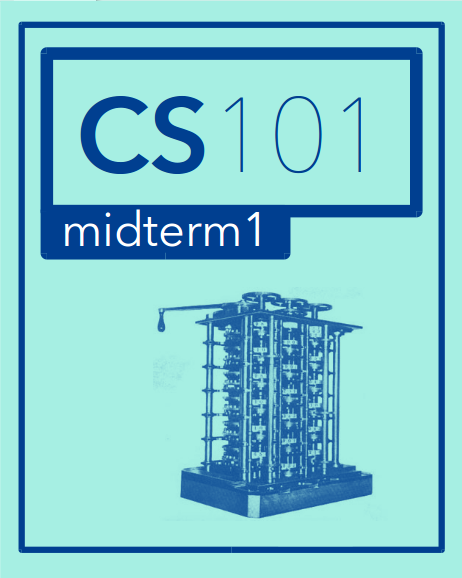
\includegraphics[width=2in]{../img/midterm1-header.png}
\end{center}

\bigskip
\noindent
\begin{itemize}
\item \textbf{Be sure to enter your \underline{NetID} and \underline{the code below} on your Scantron}.
\item Do not turn this page until instructed to do so.
\item There are 30 questions, worth 1 point each.
\item Each question has only \textbf{one} correct answer.
\item You must not communicate with other students during this test.
\item No books, notes, or electronic devices are permitted.
\item This is a 60-minute exam.
\item There are several different versions of this exam.
\end{itemize}

\bigskip\bigskip
\noindent
\textbf{\Large 1. Fill in your information:}

\bigskip
{\Large\bf
\begin{tabular}{ll}
Full Name: & \underbar{\hskip 8cm} \\[0.5em]
UIN (Student Number): & \underbar{\hskip 8cm} \\[0.5em]
NetID: & \underbar{\hskip 8cm}
\end{tabular}
}

\bigskip
\bigskip
\noindent
\textbf{\Large 2. Fill in the following answers on the Scantron form:}

%%%%%%%%%%%%%%%%%%%%%%%%%%%%%%%%%%%%%%%%%%%%%%%%%%%%%%%%%
%%%%%%%%%%%%%%%%%%%%%%%%%%%%%%%%%%%%%%%%%%%%%%%%%%%%%%%%%

\begin{enumerate}
\item[92.] B
\item[93.] B
\item[94.] B
\item[95.] B
\item[96.] D
\end{enumerate}

\newpage

% Zone 1


%%%%%%%%%%%%%%%%%%%%%%%%%%%%%%%%%%%%%%%%%%%%%%%%%%%%%%%%%



\newpage
\noindent
1. (1 point)
Evaluate the following expression:
\begin{verbatim}
len("ABCD"[0:3])
\end{verbatim}
What value is produced?


\begin{enumerate}
\item[(A)] $\bigstar$ 
3

\item[(B)]
4

\item[(C)]
1

\item[(D)]
2

\end{enumerate}

\vspace*{2em}
\hrule
\vspace{2em}

\noindent {\bf Solution.} 
\vspace{2em}
\hrule height 2pt


\newpage
\noindent
2. (1 point)
Consider the following program:
\begin{verbatim}
x="KING ARTHUR-MORGANA LEFAY-SIR BEDIVERE".split("-")
y=x
y.reverse()
\end{verbatim}
What is the \textbf{value} of \texttt{x} after this program is executed?


\begin{enumerate}
\item[(A)]
\begin{verbatim}['KING', 'ARTHUR-MORGANA', 'LEFAY-SIR', 'BEDIVERE']\end{verbatim}

\item[(B)] $\bigstar$ 
\begin{verbatim}['SIR BEDIVERE', 'MORGANA LEFAY', 'KING ARTHUR']\end{verbatim}

\item[(C)]
\begin{verbatim}['BEDIVERE', 'LEFAY-SIR', 'ARTHUR-MORGANA', 'KING']\end{verbatim}

\item[(D)]
\begin{verbatim}None\end{verbatim}

\item[(E)]
\begin{verbatim}['KING ARTHUR', 'MORGANA LEFAY', 'SIR BEDIVERE']\end{verbatim}

\end{enumerate}

\vspace*{2em}
\hrule
\vspace{2em}

\noindent {\bf Solution.} 
\vspace{2em}
\hrule height 2pt


\newpage
\noindent
3. (1 point)
Consider the following program.
\begin{verbatim}
s="ABCBA"
x=0
y=len(s)-1
while s[x]==s[y] and x<y:
    x+=1
    y-=1
\end{verbatim}
After it is run, what is the final \textbf{value} of \texttt{x}?


\begin{enumerate}
\item[(A)]
\begin{verbatim}0\end{verbatim}

\item[(B)]
\begin{verbatim}3\end{verbatim}

\item[(C)]
\begin{verbatim}4\end{verbatim}

\item[(D)]
\begin{verbatim}1\end{verbatim}

\item[(E)] $\bigstar$ 
\begin{verbatim}2\end{verbatim}

\end{enumerate}

\vspace*{2em}
\hrule
\vspace{2em}

\noindent {\bf Solution.} 
\vspace{2em}
\hrule height 2pt


\newpage
\noindent
4. (1 point)
Consider the following incomplete Python program.
\begin{verbatim}
s="".join(["1","0","2","1"])
x=0
for i in range(len(s)-1):
    x+=int(???)
\end{verbatim}
What should replace the three question marks so the resulting value of \texttt{x} is 33?


\begin{enumerate}
\item[(A)]
\begin{verbatim}s[i+1:i+2]\end{verbatim}

\item[(B)]
\begin{verbatim}s[i:i+1]\end{verbatim}

\item[(C)] $\bigstar$ 
\begin{verbatim}s[i:i+2]\end{verbatim}

\item[(D)]
\begin{verbatim}s[i:i-1]\end{verbatim}

\end{enumerate}

\vspace*{2em}
\hrule
\vspace{2em}

\noindent {\bf Solution.} 
\vspace{2em}
\hrule height 2pt


\newpage
\noindent
5. (1 point)
Consider the following program:
\begin{verbatim}
x=0
for i in range(2,8):
    if i%3==0:
        x+=3
    elif i%2==0:
        x+=2
    else:
        x+=1
\end{verbatim}
What is the \textbf{value} of \texttt{x} after this program is executed?


\begin{enumerate}
\item[(A)]
\begin{verbatim}14\end{verbatim}

\item[(B)]
\begin{verbatim}10\end{verbatim}

\item[(C)]
\begin{verbatim}13\end{verbatim}

\item[(D)] $\bigstar$ 
\begin{verbatim}12\end{verbatim}

\item[(E)]
\begin{verbatim}11\end{verbatim}

\end{enumerate}

\vspace*{2em}
\hrule
\vspace{2em}

\noindent {\bf Solution.} 
\vspace{2em}
\hrule height 2pt


\newpage
\noindent
6. (1 point)
Consider the following program:
\begin{verbatim}
x=str(1.2)*2
\end{verbatim}
What is the \textbf{value} of \texttt{x} after this program is executed?


\begin{enumerate}
\item[(A)]
None of the other answers are correct.

\item[(B)]
\begin{verbatim}"2.4"\end{verbatim}

\item[(C)]
\begin{verbatim}2.4\end{verbatim}

\item[(D)]
\begin{verbatim}"1.2*2"\end{verbatim}

\item[(E)] $\bigstar$ 
\begin{verbatim}"1.21.2"\end{verbatim}

\end{enumerate}

\vspace*{2em}
\hrule
\vspace{2em}

\noindent {\bf Solution.} 
\vspace{2em}
\hrule height 2pt


\newpage
\noindent
7. (1 point)
For this problem, you should compose a function which accomplishes a given task using the available code blocks arranged in the correct functional order.  \emph{We ignore indentation for this problem.}

\texttt{find\_max} should accept a \texttt{list} and return the value of the maximum item in the \texttt{list}.  (\texttt{None} is always the lowest value in any numeric comparison, so you may use it as an initializer.)

\begin{verbatim}
def find_max(my_list):
\end{verbatim}

\begin{enumerate}[1]
\item \texttt{max\_val = i}
\item \texttt{max\_val = None}
\item \texttt{for i in range(len(my\_list)):}
\item \texttt{if i > max\_val:}
\item \texttt{max\_val = my\_list[i]}
\item \texttt{return max\_val}
\item \texttt{for i in range(my\_list):}
\item \texttt{if my\_list[i] > max\_val:}
\item \texttt{print(max\_val)}
\end{enumerate}



\begin{enumerate}
\item[(A)]
2, 3, 4, 1, 6

\item[(B)]
2, 3, 8, 1, 6

\item[(C)] $\bigstar$ 
2, 3, 8, 5, 6

\item[(D)]
3, 2, 8, 5, 9

\item[(E)]
2, 7, 4, 5, 6

\end{enumerate}

\vspace*{2em}
\hrule
\vspace{2em}

\noindent {\bf Solution.} 
\vspace{2em}
\hrule height 2pt


\newpage
\noindent
8. (1 point)
Consider the following program:
\begin{verbatim}
s="G+R+A+I+L"
x=s.split("+")[1:-2]
\end{verbatim}
What is the \textbf{value} of \texttt{x} after this program is executed?


\begin{enumerate}
\item[(A)]
\begin{verbatim}False\end{verbatim}

\item[(B)] $\bigstar$ 
\begin{verbatim}['R','A']\end{verbatim}

\item[(C)]
\begin{verbatim}'RAI'\end{verbatim}

\item[(D)]
\begin{verbatim}3\end{verbatim}

\item[(E)]
\begin{verbatim}None\end{verbatim}

\end{enumerate}

\vspace*{2em}
\hrule
\vspace{2em}

\noindent {\bf Solution.} 
\vspace{2em}
\hrule height 2pt


\newpage
\noindent
9. (1 point)
Consider the following incomplete program.
\begin{verbatim}
sum=0
for i in range(0,100):
    ???

\end{verbatim}
The program is intended to sum all of the integers between 1 and 100 (inclusive). What should replace the three question marks to complete the program?


\begin{enumerate}
\item[(A)]
\begin{verbatim}sum+1=sum \end{verbatim}

\item[(B)] $\bigstar$ 
\begin{verbatim}sum=sum+i+1 \end{verbatim}

\item[(C)]
\begin{verbatim}sum=sum+1\end{verbatim}

\item[(D)]
\begin{verbatim}sum=sum+i \end{verbatim}

\end{enumerate}

\vspace*{2em}
\hrule
\vspace{2em}

\noindent {\bf Solution.} 
\vspace{2em}
\hrule height 2pt


\newpage
\noindent
10. (1 point)
Consider the following program:
\begin{verbatim}
x=3
a=5
if (a%3)==2:
    x=x**3
elif(a%3)==1:
    x=x**2
else:
    x=x**1
\end{verbatim}
What is the \textbf{value} of \texttt{x} after this program is executed?


\begin{enumerate}
\item[(A)]
\begin{verbatim}9\end{verbatim}

\item[(B)]
\begin{verbatim}1\end{verbatim}

\item[(C)]
None of the other answers are correct.

\item[(D)]
\begin{verbatim}3\end{verbatim}

\item[(E)] $\bigstar$ 
\begin{verbatim}27\end{verbatim}

\end{enumerate}

\vspace*{2em}
\hrule
\vspace{2em}

\noindent {\bf Solution.} 
\vspace{2em}
\hrule height 2pt


\newpage
\noindent
11. (1 point)
Consider the following program:
\begin{verbatim}
s="TRIS %i"
t="ISEU"
x=len(s) % len(t[2:-1])
\end{verbatim}
What is the \textbf{type} of \texttt{x} after this program is executed?


\begin{enumerate}
\item[(A)]
\begin{verbatim}None\end{verbatim}

\item[(B)]
\begin{verbatim}Boolean\end{verbatim}

\item[(C)]
\begin{verbatim}String\end{verbatim}

\item[(D)]
\begin{verbatim}Float\end{verbatim}

\item[(E)] $\bigstar$ 
\begin{verbatim}Integer\end{verbatim}

\end{enumerate}

\vspace*{2em}
\hrule
\vspace{2em}

\noindent {\bf Solution.} 
\vspace{2em}
\hrule height 2pt


\newpage
\noindent
12. (1 point)
Consider the following program:
\begin{verbatim}
pi="3.14159"
e="2.71828"
x=pi in pi*len(e)
\end{verbatim}
What is the \textbf{type} of \texttt{x} after this program is executed?


\begin{enumerate}
\item[(A)]
\begin{verbatim}String\end{verbatim}

\item[(B)]
\begin{verbatim}Float\end{verbatim}

\item[(C)]
\begin{verbatim}None\end{verbatim}

\item[(D)]
\begin{verbatim}Integer\end{verbatim}

\item[(E)] $\bigstar$ 
\begin{verbatim}Boolean\end{verbatim}

\end{enumerate}

\vspace*{2em}
\hrule
\vspace{2em}

\noindent {\bf Solution.} 
\vspace{2em}
\hrule height 2pt


\newpage
\noindent
13. (1 point)
Consider the following program:
\begin{verbatim}
i=3
x=2
while i < 7:
    x+=i
    i+=2
\end{verbatim}
What is the \textbf{value} of \texttt{x} after this program is executed?


\begin{enumerate}
\item[(A)]
\begin{verbatim}14\end{verbatim}

\item[(B)]
\begin{verbatim}12\end{verbatim}

\item[(C)] $\bigstar$ 
\begin{verbatim}10\end{verbatim}

\item[(D)]
\begin{verbatim}11\end{verbatim}

\item[(E)]
\begin{verbatim}13\end{verbatim}

\end{enumerate}

\vspace*{2em}
\hrule
\vspace{2em}

\noindent {\bf Solution.} 
\vspace{2em}
\hrule height 2pt


\newpage
\noindent
14. (1 point)
How can the following mathematical equation be implemented as a Python expression? Assume \verb|a|, \verb|b|, and \verb|sin| have already been defined.
$$a \sin(a^b - b)$$


\begin{enumerate}
\item[(A)]
None of the other answers are correct.

\item[(B)]
\begin{verbatim}a*sin(a^b - b)\end{verbatim}

\item[(C)]
\begin{verbatim}a*sin(b^a - b)\end{verbatim}

\item[(D)]
\begin{verbatim}a sin(a**b - b)\end{verbatim}

\item[(E)] $\bigstar$ 
\begin{verbatim}a*sin(a**b - b)\end{verbatim}

\end{enumerate}

\vspace*{2em}
\hrule
\vspace{2em}

\noindent {\bf Solution.} 
\vspace{2em}
\hrule height 2pt


\newpage
\noindent
15. (1 point)
Consider the following program:
\begin{verbatim}
def fix(s):
    a=list(s)
    a.sort()
    return ''.join(a)

x=["one","two","eleven","twelve"]
s1=fix(x[0]+x[-1])
s2=fix(x[1]+x[-2])

if s1<s2:
    x.sort()
elif s1==s2:
    x.reverse()
else:
    x.append("six")
\end{verbatim}
What is the \textbf{value} of \texttt{x} after this program is executed?


\begin{enumerate}
\item[(A)]
\begin{verbatim}['eleven', 'one', 'twelve', 'two']\end{verbatim}

\item[(B)]
\begin{verbatim}['two', 'twelve', 'one', 'eleven', 'six']\end{verbatim}

\item[(C)]
\begin{verbatim}['one', 'two', 'eleven', 'twelve']\end{verbatim}

\item[(D)]
\begin{verbatim}['one', 'two', 'eleven', 'twelve', 'six']\end{verbatim}

\item[(E)] $\bigstar$ 
\begin{verbatim}['twelve', 'eleven', 'two', 'one']\end{verbatim}

\end{enumerate}

\vspace*{2em}
\hrule
\vspace{2em}

\noindent {\bf Solution.} 
\vspace{2em}
\hrule height 2pt


\newpage
\noindent
16. (1 point)
What is the result of the following expression?
\begin{verbatim}
[ 1, 2, 3 ] * 3
\end{verbatim}


\begin{enumerate}
\item[(A)]
\begin{verbatim}[3.0, 6.0, 9.0]\end{verbatim}

\item[(B)]
\begin{verbatim}(3, 6, 9)\end{verbatim}

\item[(C)] $\bigstar$ 
\begin{verbatim}[1, 2, 3, 1, 2, 3, 1, 2, 3]\end{verbatim}

\item[(D)]
\begin{verbatim}[3, 6, 9]\end{verbatim}

\item[(E)]
\begin{verbatim}[1.0, 2.0, 3.0, 1.0, 2.0, 3.0, 1.0, 2.0, 3.0]\end{verbatim}

\end{enumerate}

\vspace*{2em}
\hrule
\vspace{2em}

\noindent {\bf Solution.} 
\vspace{2em}
\hrule height 2pt


\newpage
\noindent
17. (1 point)
Evaluate the following expression:
\begin{verbatim}
[1,2]+[len("3")]
\end{verbatim}
What value is produced?


\begin{enumerate}
\item[(A)] $\bigstar$ 
\begin{verbatim}[1,2,1]\end{verbatim}

\item[(B)]
\begin{verbatim}[1,2,3]\end{verbatim}

\item[(C)]
\begin{verbatim}[1,2,"3"]\end{verbatim}

\item[(D)]
\begin{verbatim}[1,2,1,2,1,2]\end{verbatim}

\end{enumerate}

\vspace*{2em}
\hrule
\vspace{2em}

\noindent {\bf Solution.} 
\vspace{2em}
\hrule height 2pt


\newpage
\noindent
18. (1 point)
Consider the following program.
\begin{verbatim}
x=1
i=0
while(x*x)<=9:
    i=i+(x*x)
    x=x+1
\end{verbatim}
After it is run, what is the final \textbf{value} of \texttt{x}?


\begin{enumerate}
\item[(A)]
\begin{verbatim}5\end{verbatim}

\item[(B)]
\begin{verbatim}14\end{verbatim}

\item[(C)] $\bigstar$ 
\begin{verbatim}4\end{verbatim}

\item[(D)]
\begin{verbatim}3\end{verbatim}

\item[(E)]
\begin{verbatim}30\end{verbatim}

\end{enumerate}

\vspace*{2em}
\hrule
\vspace{2em}

\noindent {\bf Solution.} 
\vspace{2em}
\hrule height 2pt


\newpage
\noindent
19. (1 point)
Consider the following program.
\begin{verbatim}
def artificing(s):
    return s*2
    return s+"%i" % 2
    return s

s=artificing("MERLIN")
\end{verbatim}
After it is run, what is the final \textbf{value} of s?


\begin{enumerate}
\item[(A)]
\begin{verbatim}"MERLIN"\end{verbatim}

\item[(B)]
\begin{verbatim}"MERLIN2"\end{verbatim}

\item[(C)]
\begin{verbatim}12\end{verbatim}

\item[(D)] $\bigstar$ 
\begin{verbatim}"MERLINMERLIN"\end{verbatim}

\item[(E)]
\begin{verbatim}None\end{verbatim}

\end{enumerate}

\vspace*{2em}
\hrule
\vspace{2em}

\noindent {\bf Solution.} 
\vspace{2em}
\hrule height 2pt


\newpage
\noindent
20. (1 point)
Consider the following program:
\begin{verbatim}
x=[1,2,3,4,5,6,7,8,9]
x=x[2:-2]
i=1
while i < 3:
    x[i]+=1
    i+=1
\end{verbatim}
What is the \textbf{value} of \texttt{x} after this program is executed?


\begin{enumerate}
\item[(A)]
\begin{verbatim}[3, 5, 6, 6, 7, 8]\end{verbatim}

\item[(B)]
\begin{verbatim}[3, 5, 6, 6]\end{verbatim}

\item[(C)]
\begin{verbatim}[2, 4, 5, 5, 6, 7]\end{verbatim}

\item[(D)]
\begin{verbatim}[2, 4, 5, 6, 6, 7]\end{verbatim}

\item[(E)] $\bigstar$ 
\begin{verbatim}[3, 5, 6, 6, 7]\end{verbatim}

\end{enumerate}

\vspace*{2em}
\hrule
\vspace{2em}

\noindent {\bf Solution.} 
\vspace{2em}
\hrule height 2pt


\newpage
\noindent
21. (1 point)
Consider the following program.
\begin{verbatim}
x=[]
for j in range(0,5):
    if (j%3)==0:
        x.append("-")
    if (j%4)==0:
        x.append("*")
\end{verbatim}
After it is run, what is the final \textbf{value} of \texttt{x}?


\begin{enumerate}
\item[(A)]
\begin{verbatim}["-","*"]\end{verbatim}

\item[(B)]
None of the other answers are correct.

\item[(C)] $\bigstar$ 
\begin{verbatim}["-","*","-","*"]\end{verbatim}

\item[(D)]
\begin{verbatim}["*","-","*"]\end{verbatim}

\item[(E)]
\begin{verbatim}["*","-","*"]\end{verbatim}

\end{enumerate}

\vspace*{2em}
\hrule
\vspace{2em}

\noindent {\bf Solution.} 
\vspace{2em}
\hrule height 2pt


\newpage
\noindent
22. (1 point)
Consider the following Python program.
\begin{verbatim}
e=[1,3,5,7,9,11]
d=[0,0,0]
for i in range(0,len(e)):
    d[i%3]+=e[i]
x=d[1]
\end{verbatim}
After it is run, what is the final \textbf{value} of \texttt{x}?


\begin{enumerate}
\item[(A)] $\bigstar$ 
\begin{verbatim}12\end{verbatim}

\item[(B)]
\begin{verbatim}8\end{verbatim}

\item[(C)]
\begin{verbatim}16\end{verbatim}

\item[(D)]
\begin{verbatim}3\end{verbatim}

\item[(E)]
\begin{verbatim}0\end{verbatim}

\end{enumerate}

\vspace*{2em}
\hrule
\vspace{2em}

\noindent {\bf Solution.} 
\vspace{2em}
\hrule height 2pt


\newpage
\noindent
23. (1 point)
Consider the following program:
\begin{verbatim}
a=3
b=4
if a==3:
    b=a
elif a==4:
    a=5
else:
    a=b
\end{verbatim}
What is the \textbf{value} of a after this program is executed?


\begin{enumerate}
\item[(A)]
\begin{verbatim}7\end{verbatim}

\item[(B)]
\begin{verbatim}5\end{verbatim}

\item[(C)]
\begin{verbatim}4\end{verbatim}

\item[(D)]
None of the other answers are correct.

\item[(E)] $\bigstar$ 
\begin{verbatim}3\end{verbatim}

\end{enumerate}

\vspace*{2em}
\hrule
\vspace{2em}

\noindent {\bf Solution.} 
\vspace{2em}
\hrule height 2pt


\newpage
\noindent
24. (1 point)
Consider the following program:
\begin{verbatim}
a=["S","T","U","P","E","F","Y"]
a=a[0:4]
a.sort()
x=""
for e in a:
    x=e+x
\end{verbatim}
What is the \textbf{value} of \texttt{x} after this program is executed?


\begin{enumerate}
\item[(A)]
None of the other answers are correct.

\item[(B)]
\begin{verbatim}"PSTU"\end{verbatim}

\item[(C)] $\bigstar$ 
\begin{verbatim}"UTSP"\end{verbatim}

\item[(D)]
\begin{verbatim}"STUP"\end{verbatim}

\item[(E)]
\begin{verbatim}"PUST"\end{verbatim}

\end{enumerate}

\vspace*{2em}
\hrule
\vspace{2em}

\noindent {\bf Solution.} 
\vspace{2em}
\hrule height 2pt


\newpage
\noindent
25. (1 point)
Consider the following program:
\begin{verbatim}
s="ECTOR"
t="GAWAIN"
x=(len(s)/(len(t)-1))+1
\end{verbatim}
What is the \textbf{type} of \texttt{x} after this program is executed?


\begin{enumerate}
\item[(A)] $\bigstar$ 
\begin{verbatim}Float\end{verbatim}

\item[(B)]
\begin{verbatim}Boolean\end{verbatim}

\item[(C)]
\begin{verbatim}String\end{verbatim}

\item[(D)]
\begin{verbatim}Integer\end{verbatim}

\item[(E)]
\begin{verbatim}None\end{verbatim}

\end{enumerate}

\vspace*{2em}
\hrule
\vspace{2em}

\noindent {\bf Solution.} 
\vspace{2em}
\hrule height 2pt


\newpage
\noindent
26. (1 point)
Consider the following program:
\begin{verbatim}
x=[1,2,3]
def f(a):
    s=""
    a.append(4)
    for i in a:
        s+=str(i)
    return s

x.append(f(x))
\end{verbatim}
What is the \textbf{value} of \texttt{x} after this program is executed?


\begin{enumerate}
\item[(A)] $\bigstar$ 
\begin{verbatim}[1, 2, 3, 4, '1234']\end{verbatim}

\item[(B)]
\begin{verbatim}[1, 2, 3, '1234']\end{verbatim}

\item[(C)]
\begin{verbatim}[1, 2, 3, '123']\end{verbatim}

\item[(D)]
\begin{verbatim}[1, 2, 3, 10]\end{verbatim}

\item[(E)]
\begin{verbatim}[1, 2, 3]\end{verbatim}

\end{enumerate}

\vspace*{2em}
\hrule
\vspace{2em}

\noindent {\bf Solution.} 
\vspace{2em}
\hrule height 2pt


\newpage
\noindent
27. (1 point)
Consider the following program:
\begin{verbatim}
a=["merlin","sir agravaine","king pellinore"]
b=[ ]
for i in range(0,3):
    b.append(a[0-i].title())
\end{verbatim}
What is the \textbf{value} of b after this program is executed?


\begin{enumerate}
\item[(A)]
\begin{verbatim}['King Pellinore', 'Sir Agravaine', 'Merlin']\end{verbatim}

\item[(B)]
\begin{verbatim}['King Pellinore', 'Sir Agravaine']\end{verbatim}

\item[(C)]
\begin{verbatim}['Sir Agravaine', 'King Pellinore']\end{verbatim}

\item[(D)]
\begin{verbatim}[ ]\end{verbatim}

\item[(E)] $\bigstar$ 
\begin{verbatim}['Merlin', 'King Pellinore', 'Sir Agravaine']\end{verbatim}

\end{enumerate}

\vspace*{2em}
\hrule
\vspace{2em}

\noindent {\bf Solution.} 
\vspace{2em}
\hrule height 2pt


\newpage
\noindent
28. (1 point)
Consider the following incomplete function.
\begin{verbatim}
def isdivisible(m,n):
    if ???:
        return False
    else:
        return True
\end{verbatim}
The function is intended to return True if the input parameter m is evenly divisible by the parameter n and False otherwise. For example, \verb|isdivisible(4,2)| should return \verb|True|, but \verb|isdivisible(5,3)| should return \verb|False|. What should replace the three question marks to complete the function?


\begin{enumerate}
\item[(A)]
\begin{verbatim}(m // n) != 0 \end{verbatim}

\item[(B)]
\begin{verbatim}(n // m) == 0 \end{verbatim}

\item[(C)] $\bigstar$ 
\begin{verbatim}(m % n) != 0 \end{verbatim}

\item[(D)]
\begin{verbatim}(n % m) == 0 \end{verbatim}

\end{enumerate}

\vspace*{2em}
\hrule
\vspace{2em}

\noindent {\bf Solution.} 
\vspace{2em}
\hrule height 2pt


\newpage
\noindent
29. (1 point)
Consider the following program.
\begin{verbatim}
kay = 2
wart = 3

def knight(kay,wart):
    wart += 2
    kay += 3
    return wart + kay

kay = knight(wart, kay) + knight(kay, wart)
\end{verbatim}
After it is run, what is the final \textbf{value} of \texttt{kay}?


\begin{enumerate}
\item[(A)]
\begin{verbatim}5\end{verbatim}

\item[(B)]
\begin{verbatim}3\end{verbatim}

\item[(C)] $\bigstar$ 
None of the other answers are correct.

\item[(D)]
\begin{verbatim}2\end{verbatim}

\end{enumerate}

\vspace*{2em}
\hrule
\vspace{2em}

\noindent {\bf Solution.} 
\vspace{2em}
\hrule height 2pt


\newpage
\noindent
30. (1 point)
Consider the following program:
\begin{verbatim}
s="Calvin"
i=0
x=-1
while i<len(s):
    if s[i]=='b':
        x=i
    i+=1
\end{verbatim}
What is the \textbf{value} of \texttt{x} after this program is executed?


\begin{enumerate}
\item[(A)]
\begin{verbatim}0\end{verbatim}

\item[(B)]
\begin{verbatim}5\end{verbatim}

\item[(C)]
\begin{verbatim}3\end{verbatim}

\item[(D)] $\bigstar$ 
\begin{verbatim}-1\end{verbatim}

\item[(E)]
\begin{verbatim}6\end{verbatim}

\end{enumerate}

\vspace*{2em}
\hrule
\vspace{2em}

\noindent {\bf Solution.} 
\vspace{2em}
\hrule height 2pt

%%%%%%%%%%%%%%%%%%%%%%%%%%%%%%%%%%%%%%%%%%%%%%%%%%%%%%%%%%%%%%%%%%%%%%
%%%%%%%%%%%%%%%%%%%%%%%%%%%%%%%%%%%%%%%%%%%%%%%%%%%%%%%%%%%%%%%%%%%%%%
%%%%%%%%%%%%%%%%%%%%%%%%%%%%%%%%%%%%%%%%%%%%%%%%%%%%%%%%%%%%%%%%%%%%%%
%%%%%%%%%%%%%%%%%%%%%%%%%%%%%%%%%%%%%%%%%%%%%%%%%%%%%%%%%%%%%%%%%%%%%%
% Exam number 33

\message{Exam 33/50}
\cleardoublepage
\setcounter{page}{1}


\begin{center}
%\textbf{\Large CS 101 Midterm \#1}
%
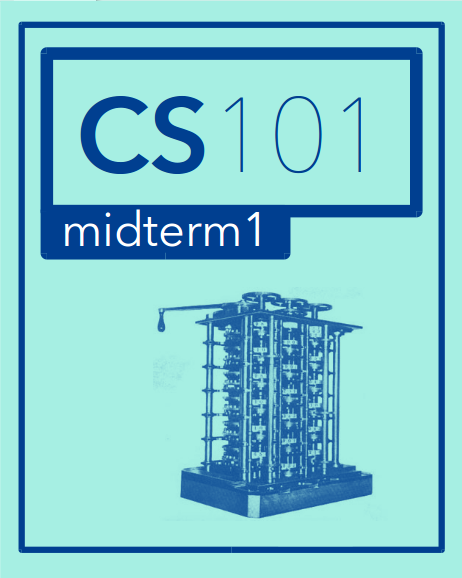
\includegraphics[width=2in]{../img/midterm1-header.png}
\end{center}

\bigskip
\noindent
\begin{itemize}
\item \textbf{Be sure to enter your \underline{NetID} and \underline{the code below} on your Scantron}.
\item Do not turn this page until instructed to do so.
\item There are 30 questions, worth 1 point each.
\item Each question has only \textbf{one} correct answer.
\item You must not communicate with other students during this test.
\item No books, notes, or electronic devices are permitted.
\item This is a 60-minute exam.
\item There are several different versions of this exam.
\end{itemize}

\bigskip\bigskip
\noindent
\textbf{\Large 1. Fill in your information:}

\bigskip
{\Large\bf
\begin{tabular}{ll}
Full Name: & \underbar{\hskip 8cm} \\[0.5em]
UIN (Student Number): & \underbar{\hskip 8cm} \\[0.5em]
NetID: & \underbar{\hskip 8cm}
\end{tabular}
}

\bigskip
\bigskip
\noindent
\textbf{\Large 2. Fill in the following answers on the Scantron form:}

%%%%%%%%%%%%%%%%%%%%%%%%%%%%%%%%%%%%%%%%%%%%%%%%%%%%%%%%%
%%%%%%%%%%%%%%%%%%%%%%%%%%%%%%%%%%%%%%%%%%%%%%%%%%%%%%%%%

\begin{enumerate}
\item[92.] C
\item[93.] B
\item[94.] B
\item[95.] C
\item[96.] E
\end{enumerate}

\newpage

% Zone 1


%%%%%%%%%%%%%%%%%%%%%%%%%%%%%%%%%%%%%%%%%%%%%%%%%%%%%%%%%



\newpage
\noindent
1. (1 point)
Consider the following incomplete Python program.
\begin{verbatim}
s="".join(["2","2","0","1"])
x=0
for i in range(len(s)-1):
    x+=int(???)
\end{verbatim}
What should replace the three question marks so the resulting value of \texttt{x} is 43?


\begin{enumerate}
\item[(A)]
\begin{verbatim}s[i+1:i+2]\end{verbatim}

\item[(B)]
\begin{verbatim}s[i:i+1]\end{verbatim}

\item[(C)]
\begin{verbatim}s[i:i-1]\end{verbatim}

\item[(D)] $\bigstar$ 
\begin{verbatim}s[i:i+2]\end{verbatim}

\end{enumerate}

\vspace*{2em}
\hrule
\vspace{2em}

\noindent {\bf Solution.} 
\vspace{2em}
\hrule height 2pt


\newpage
\noindent
2. (1 point)
How can the following mathematical equation be implemented as a Python expression? Assume \verb|a|, \verb|b|, and \verb|sin| have already been defined.
$$a \sin(a^b - b)$$


\begin{enumerate}
\item[(A)]
None of the other answers are correct.

\item[(B)]
\begin{verbatim}a sin(a**b - b)\end{verbatim}

\item[(C)] $\bigstar$ 
\begin{verbatim}a*sin(a**b - b)\end{verbatim}

\item[(D)]
\begin{verbatim}a*sin(a^b - b)\end{verbatim}

\item[(E)]
\begin{verbatim}a*sin(b^a - b)\end{verbatim}

\end{enumerate}

\vspace*{2em}
\hrule
\vspace{2em}

\noindent {\bf Solution.} 
\vspace{2em}
\hrule height 2pt


\newpage
\noindent
3. (1 point)
Consider the following program:
\begin{verbatim}
x=0
for i in range(2,8):
    if i%3==0:
        x+=3
    elif i%2==0:
        x+=2
    else:
        x+=1
\end{verbatim}
What is the \textbf{value} of \texttt{x} after this program is executed?


\begin{enumerate}
\item[(A)]
\begin{verbatim}10\end{verbatim}

\item[(B)] $\bigstar$ 
\begin{verbatim}12\end{verbatim}

\item[(C)]
\begin{verbatim}13\end{verbatim}

\item[(D)]
\begin{verbatim}11\end{verbatim}

\item[(E)]
\begin{verbatim}14\end{verbatim}

\end{enumerate}

\vspace*{2em}
\hrule
\vspace{2em}

\noindent {\bf Solution.} 
\vspace{2em}
\hrule height 2pt


\newpage
\noindent
4. (1 point)
Consider the following program:
\begin{verbatim}
s="Hobbes"
i=0
x=-1
while i<len(s):
    if s[i]=='b':
        x=i
    i+=1
\end{verbatim}
What is the \textbf{value} of \texttt{x} after this program is executed?


\begin{enumerate}
\item[(A)]
\begin{verbatim}2\end{verbatim}

\item[(B)] $\bigstar$ 
\begin{verbatim}3\end{verbatim}

\item[(C)]
\begin{verbatim}-1\end{verbatim}

\item[(D)]
\begin{verbatim}4\end{verbatim}

\item[(E)]
\begin{verbatim}5\end{verbatim}

\end{enumerate}

\vspace*{2em}
\hrule
\vspace{2em}

\noindent {\bf Solution.} 
\vspace{2em}
\hrule height 2pt


\newpage
\noindent
5. (1 point)
Consider the following Python program.
\begin{verbatim}
e=[1,3,5,7,9,11]
d=[0,0,0]
for i in range(0,len(e)):
    d[i%3]+=e[i]
x=d[1]
\end{verbatim}
After it is run, what is the final \textbf{value} of \texttt{x}?


\begin{enumerate}
\item[(A)]
\begin{verbatim}0\end{verbatim}

\item[(B)]
\begin{verbatim}16\end{verbatim}

\item[(C)] $\bigstar$ 
\begin{verbatim}12\end{verbatim}

\item[(D)]
\begin{verbatim}3\end{verbatim}

\item[(E)]
\begin{verbatim}8\end{verbatim}

\end{enumerate}

\vspace*{2em}
\hrule
\vspace{2em}

\noindent {\bf Solution.} 
\vspace{2em}
\hrule height 2pt


\newpage
\noindent
6. (1 point)
Evaluate the following expression:
\begin{verbatim}
len("ABCD"[0:3])
\end{verbatim}
What value is produced?


\begin{enumerate}
\item[(A)]
1

\item[(B)]
2

\item[(C)] $\bigstar$ 
3

\item[(D)]
4

\end{enumerate}

\vspace*{2em}
\hrule
\vspace{2em}

\noindent {\bf Solution.} 
\vspace{2em}
\hrule height 2pt


\newpage
\noindent
7. (1 point)
\begin{verbatim}
x=str(3)+"str(3)"
\end{verbatim}
What is the \textbf{value} of \texttt{x} after this program is executed?


\begin{enumerate}
\item[(A)]
\begin{verbatim}33\end{verbatim}

\item[(B)] $\bigstar$ 
\begin{verbatim}"3str(3)"\end{verbatim}

\item[(C)]
\begin{verbatim}"33"\end{verbatim}

\item[(D)]
None of the other answers are correct.

\item[(E)]
\begin{verbatim}"333"\end{verbatim}

\end{enumerate}

\vspace*{2em}
\hrule
\vspace{2em}

\noindent {\bf Solution.} 
\vspace{2em}
\hrule height 2pt


\newpage
\noindent
8. (1 point)
Consider the following program:
\begin{verbatim}
s="-B-O-R-S-"
x=s.split("-")[2:-2]
\end{verbatim}
What is the \textbf{value} of \texttt{x} after this program is executed?


\begin{enumerate}
\item[(A)]
\begin{verbatim}None\end{verbatim}

\item[(B)]
\begin{verbatim}''\end{verbatim}

\item[(C)] $\bigstar$ 
\begin{verbatim}['O', 'R']\end{verbatim}

\item[(D)]
\begin{verbatim}'ORS'\end{verbatim}

\item[(E)]
\begin{verbatim}False\end{verbatim}

\end{enumerate}

\vspace*{2em}
\hrule
\vspace{2em}

\noindent {\bf Solution.} 
\vspace{2em}
\hrule height 2pt


\newpage
\noindent
9. (1 point)
For this problem, you should compose a function which accomplishes a given task using the available code blocks arranged in the correct functional order.  \emph{We ignore indentation for this problem.}

\texttt{find\_max} should accept a \texttt{list} and return the value of the maximum item in the \texttt{list}.  (\texttt{None} is always the lowest value in any numeric comparison, so you may use it as an initializer.)

\begin{verbatim}
def find_max(my_list):
\end{verbatim}

\begin{enumerate}[1]
\item \texttt{max\_val = i}
\item \texttt{max\_val = None}
\item \texttt{for i in range(len(my\_list)):}
\item \texttt{if i > max\_val:}
\item \texttt{max\_val = my\_list[i]}
\item \texttt{return max\_val}
\item \texttt{for i in range(my\_list):}
\item \texttt{if my\_list[i] > max\_val:}
\item \texttt{print(max\_val)}
\end{enumerate}



\begin{enumerate}
\item[(A)]
2, 3, 8, 1, 6

\item[(B)]
3, 2, 8, 5, 9

\item[(C)] $\bigstar$ 
2, 3, 8, 5, 6

\item[(D)]
2, 3, 4, 1, 6

\item[(E)]
2, 7, 4, 5, 6

\end{enumerate}

\vspace*{2em}
\hrule
\vspace{2em}

\noindent {\bf Solution.} 
\vspace{2em}
\hrule height 2pt


\newpage
\noindent
10. (1 point)
Consider the following program:
\begin{verbatim}
s="ECTOR"
t="GAWAIN"
x=(len(s)+len(t)) < 4 and s in t
\end{verbatim}
What is the \textbf{type} of \texttt{x} after this program is executed?


\begin{enumerate}
\item[(A)]
\begin{verbatim}Integer\end{verbatim}

\item[(B)] $\bigstar$ 
\begin{verbatim}Boolean\end{verbatim}

\item[(C)]
\begin{verbatim}Float\end{verbatim}

\item[(D)]
\begin{verbatim}String\end{verbatim}

\item[(E)]
\begin{verbatim}None\end{verbatim}

\end{enumerate}

\vspace*{2em}
\hrule
\vspace{2em}

\noindent {\bf Solution.} 
\vspace{2em}
\hrule height 2pt


\newpage
\noindent
11. (1 point)
Consider the following program:
\begin{verbatim}
x=[2,3,4,5,6,7,8,9]
x=x[2:-2]
i=1
while i <= 3:
    x[i]+=1
    i+=1
\end{verbatim}
What is the \textbf{value} of \texttt{x} after this program is executed?


\begin{enumerate}
\item[(A)]
\begin{verbatim}[3, 4, 6, 7, 8]\end{verbatim}

\item[(B)]
\begin{verbatim}[2, 4, 6, 6]\end{verbatim}

\item[(C)] $\bigstar$ 
\begin{verbatim}[4, 6, 7, 8]\end{verbatim}

\item[(D)]
\begin{verbatim}[4, 6, 7]\end{verbatim}

\item[(E)]
\begin{verbatim}[4, 6, 7, 7]\end{verbatim}

\end{enumerate}

\vspace*{2em}
\hrule
\vspace{2em}

\noindent {\bf Solution.} 
\vspace{2em}
\hrule height 2pt


\newpage
\noindent
12. (1 point)
Consider the following program:
\begin{verbatim}
def fix(s):
    a=list(s)
    a.sort()
    return ''.join(a)

x=["one","two","eleven","twelve"]
s1=fix(x[0]+x[-1])
s2=fix(x[1]+x[-2])

if s1<s2:
    x.sort()
elif s1==s2:
    x.reverse()
else:
    x.append("six")
\end{verbatim}
What is the \textbf{value} of \texttt{x} after this program is executed?


\begin{enumerate}
\item[(A)] $\bigstar$ 
\begin{verbatim}['twelve', 'eleven', 'two', 'one']\end{verbatim}

\item[(B)]
\begin{verbatim}['one', 'two', 'eleven', 'twelve']\end{verbatim}

\item[(C)]
\begin{verbatim}['eleven', 'one', 'twelve', 'two']\end{verbatim}

\item[(D)]
\begin{verbatim}['two', 'twelve', 'one', 'eleven', 'six']\end{verbatim}

\item[(E)]
\begin{verbatim}['one', 'two', 'eleven', 'twelve', 'six']\end{verbatim}

\end{enumerate}

\vspace*{2em}
\hrule
\vspace{2em}

\noindent {\bf Solution.} 
\vspace{2em}
\hrule height 2pt


\newpage
\noindent
13. (1 point)
Consider the following program.
\begin{verbatim}
x=[]
for j in range(0,5):
    if (j%3)==0:
        x.append("-")
    if (j%4)==0:
        x.append("*")
\end{verbatim}
After it is run, what is the final \textbf{value} of \texttt{x}?


\begin{enumerate}
\item[(A)] $\bigstar$ 
\begin{verbatim}["-","*","-","*"]\end{verbatim}

\item[(B)]
None of the other answers are correct.

\item[(C)]
\begin{verbatim}["*","-","*"]\end{verbatim}

\item[(D)]
\begin{verbatim}["-","*"]\end{verbatim}

\item[(E)]
\begin{verbatim}["*","-","*"]\end{verbatim}

\end{enumerate}

\vspace*{2em}
\hrule
\vspace{2em}

\noindent {\bf Solution.} 
\vspace{2em}
\hrule height 2pt


\newpage
\noindent
14. (1 point)
Consider the following program:
\begin{verbatim}
s="TRIS %i"
t="ISEU"
x=len(s) % len(t[2:-1])
\end{verbatim}
What is the \textbf{type} of \texttt{x} after this program is executed?


\begin{enumerate}
\item[(A)]
\begin{verbatim}None\end{verbatim}

\item[(B)] $\bigstar$ 
\begin{verbatim}Integer\end{verbatim}

\item[(C)]
\begin{verbatim}Float\end{verbatim}

\item[(D)]
\begin{verbatim}Boolean\end{verbatim}

\item[(E)]
\begin{verbatim}String\end{verbatim}

\end{enumerate}

\vspace*{2em}
\hrule
\vspace{2em}

\noindent {\bf Solution.} 
\vspace{2em}
\hrule height 2pt


\newpage
\noindent
15. (1 point)
Consider the following incomplete function.
\begin{verbatim}
def ismultiple(m,n):
    if ???:
        return False
    else:
        return True
\end{verbatim}
The function is intended to return True if the input parameter m is a multiple of parameter n and False otherwise. For example, \verb|ismultiple(4,2)| should return \verb|True|, but \verb|ismultiple(5,3)| should return \verb|False|. What should replace the three question marks to complete the function?


\begin{enumerate}
\item[(A)] $\bigstar$ 
\begin{verbatim}(m % n) != 0 \end{verbatim}

\item[(B)]
\begin{verbatim}(n % m) == 0 \end{verbatim}

\item[(C)]
\begin{verbatim}(m // n) != 0 \end{verbatim}

\item[(D)]
\begin{verbatim}(n // m) == 0 \end{verbatim}

\end{enumerate}

\vspace*{2em}
\hrule
\vspace{2em}

\noindent {\bf Solution.} 
\vspace{2em}
\hrule height 2pt


\newpage
\noindent
16. (1 point)
Consider the following program.
\begin{verbatim}
def artificing(s):
    return s+"%i" % 2
    return s*2
    return s

s=artificing("MERLIN")
\end{verbatim}
After it is run, what is the final \textbf{value} of s?


\begin{enumerate}
\item[(A)]
\begin{verbatim}"MERLINMERLIN"\end{verbatim}

\item[(B)]
\begin{verbatim}"MERLIN%i"\end{verbatim}

\item[(C)]
\begin{verbatim}0\end{verbatim}

\item[(D)] $\bigstar$ 
\begin{verbatim}"MERLIN2"\end{verbatim}

\item[(E)]
\begin{verbatim}None\end{verbatim}

\end{enumerate}

\vspace*{2em}
\hrule
\vspace{2em}

\noindent {\bf Solution.} 
\vspace{2em}
\hrule height 2pt


\newpage
\noindent
17. (1 point)
Consider the following incomplete program.
\begin{verbatim}
sum=0
???:
    sum=sum+i

\end{verbatim}
The program is intended to sum all of the integers between 1 and 100 (inclusive). What should replace the three question marks to complete the program?


\begin{enumerate}
\item[(A)]
\begin{verbatim}while i<=100 \end{verbatim}

\item[(B)]
\begin{verbatim}for i in range(0,100)\end{verbatim}

\item[(C)] $\bigstar$ 
\begin{verbatim}for i in range(1,101) \end{verbatim}

\item[(D)]
\begin{verbatim}while i in range(100)\end{verbatim}

\end{enumerate}

\vspace*{2em}
\hrule
\vspace{2em}

\noindent {\bf Solution.} 
\vspace{2em}
\hrule height 2pt


\newpage
\noindent
18. (1 point)
Consider the following program:
\begin{verbatim}
a=3
b=4
if a==3:
    a=b
elif a==4:
    a=5
else:
    b=a
\end{verbatim}
What is the \textbf{value} of a after this program is executed?


\begin{enumerate}
\item[(A)]
\begin{verbatim}5\end{verbatim}

\item[(B)]
None of the other answers are correct.

\item[(C)]
\begin{verbatim}7\end{verbatim}

\item[(D)]
\begin{verbatim}3\end{verbatim}

\item[(E)] $\bigstar$ 
\begin{verbatim}4\end{verbatim}

\end{enumerate}

\vspace*{2em}
\hrule
\vspace{2em}

\noindent {\bf Solution.} 
\vspace{2em}
\hrule height 2pt


\newpage
\noindent
19. (1 point)
Consider the following program:
\begin{verbatim}
a=["merlin","sir agravaine","king pellinore"]
b=[ ]
for i in range(0,3):
    b.append(a[0-i].title())
\end{verbatim}
What is the \textbf{value} of b after this program is executed?


\begin{enumerate}
\item[(A)]
\begin{verbatim}['King Pellinore', 'Sir Agravaine']\end{verbatim}

\item[(B)] $\bigstar$ 
\begin{verbatim}['Merlin', 'King Pellinore', 'Sir Agravaine']\end{verbatim}

\item[(C)]
\begin{verbatim}['King Pellinore', 'Sir Agravaine', 'Merlin']\end{verbatim}

\item[(D)]
\begin{verbatim}[ ]\end{verbatim}

\item[(E)]
\begin{verbatim}['Sir Agravaine', 'King Pellinore']\end{verbatim}

\end{enumerate}

\vspace*{2em}
\hrule
\vspace{2em}

\noindent {\bf Solution.} 
\vspace{2em}
\hrule height 2pt


\newpage
\noindent
20. (1 point)
Consider the following program:
\begin{verbatim}
a=["A","C","C","I","O"]
a.sort()
a[0]=a[-1]
x=""
for e in a:
    x=x+e
\end{verbatim}
What is the \textbf{value} of \texttt{x} after this program is executed?


\begin{enumerate}
\item[(A)]
\begin{verbatim}"ICCOI"\end{verbatim}

\item[(B)] $\bigstar$ 
\begin{verbatim}"OCCIO"\end{verbatim}

\item[(C)]
None of the other answers are correct.

\item[(D)]
\begin{verbatim}"ACCIA"\end{verbatim}

\item[(E)]
\begin{verbatim}"ACCOA"\end{verbatim}

\end{enumerate}

\vspace*{2em}
\hrule
\vspace{2em}

\noindent {\bf Solution.} 
\vspace{2em}
\hrule height 2pt


\newpage
\noindent
21. (1 point)
Consider the following program:
\begin{verbatim}
x=[1,2,3]
def f(a):
    s=""
    a.append(4)
    for i in a:
        s+=str(i)
    return s

x.append(f(x))
\end{verbatim}
What is the \textbf{value} of \texttt{x} after this program is executed?


\begin{enumerate}
\item[(A)]
\begin{verbatim}[1, 2, 3]\end{verbatim}

\item[(B)]
\begin{verbatim}[1, 2, 3, '1234']\end{verbatim}

\item[(C)]
\begin{verbatim}[1, 2, 3, 10]\end{verbatim}

\item[(D)] $\bigstar$ 
\begin{verbatim}[1, 2, 3, 4, '1234']\end{verbatim}

\item[(E)]
\begin{verbatim}[1, 2, 3, '123']\end{verbatim}

\end{enumerate}

\vspace*{2em}
\hrule
\vspace{2em}

\noindent {\bf Solution.} 
\vspace{2em}
\hrule height 2pt


\newpage
\noindent
22. (1 point)
Consider the following program.
\begin{verbatim}
s="ABCBA"
x=0
y=len(s)-1
while s[x]==s[y] and x<=y:
    x+=1
    y-=1
\end{verbatim}
After it is run, what is the final \textbf{value} of \texttt{x}?


\begin{enumerate}
\item[(A)]
\begin{verbatim}4\end{verbatim}

\item[(B)]
\begin{verbatim}2\end{verbatim}

\item[(C)]
\begin{verbatim}1\end{verbatim}

\item[(D)] $\bigstar$ 
\begin{verbatim}3\end{verbatim}

\item[(E)]
\begin{verbatim}0\end{verbatim}

\end{enumerate}

\vspace*{2em}
\hrule
\vspace{2em}

\noindent {\bf Solution.} 
\vspace{2em}
\hrule height 2pt


\newpage
\noindent
23. (1 point)
Consider the following program.
\begin{verbatim}
kay = 2
wart = 3

def knight(kay,wart):
    wart += 2
    kay += 3
    return wart + kay

wart = knight(kay, kay) + knight(wart, wart)
\end{verbatim}
After it is run, what is the final \textbf{value} of \texttt{wart}?


\begin{enumerate}
\item[(A)]
\begin{verbatim}3\end{verbatim}

\item[(B)]
\begin{verbatim}5\end{verbatim}

\item[(C)] $\bigstar$ 
None of the other answers are correct.

\item[(D)]
\begin{verbatim}2\end{verbatim}

\end{enumerate}

\vspace*{2em}
\hrule
\vspace{2em}

\noindent {\bf Solution.} 
\vspace{2em}
\hrule height 2pt


\newpage
\noindent
24. (1 point)
Consider the following program:
\begin{verbatim}
i=2
x=3
while i < 7:
    x+=i
    i+=2
\end{verbatim}
What is the \textbf{value} of \texttt{x} after this program is executed?


\begin{enumerate}
\item[(A)]
\begin{verbatim}12\end{verbatim}

\item[(B)]
\begin{verbatim}13\end{verbatim}

\item[(C)]
\begin{verbatim}14\end{verbatim}

\item[(D)]
\begin{verbatim}11\end{verbatim}

\item[(E)] $\bigstar$ 
\begin{verbatim}15\end{verbatim}

\end{enumerate}

\vspace*{2em}
\hrule
\vspace{2em}

\noindent {\bf Solution.} 
\vspace{2em}
\hrule height 2pt


\newpage
\noindent
25. (1 point)
Consider the following program:
\begin{verbatim}
pi="3.14159"
e="2.71828"
x=pi*len(e)+pi
\end{verbatim}
What is the \textbf{type} of \texttt{x} after this program is executed?


\begin{enumerate}
\item[(A)]
\begin{verbatim}Boolean\end{verbatim}

\item[(B)]
\begin{verbatim}Float\end{verbatim}

\item[(C)]
\begin{verbatim}Integer\end{verbatim}

\item[(D)] $\bigstar$ 
\begin{verbatim}String\end{verbatim}

\item[(E)]
\begin{verbatim}None\end{verbatim}

\end{enumerate}

\vspace*{2em}
\hrule
\vspace{2em}

\noindent {\bf Solution.} 
\vspace{2em}
\hrule height 2pt


\newpage
\noindent
26. (1 point)
Evaluate the following expression:
\begin{verbatim}
[1,2]*len("3")
\end{verbatim}
What value is produced?


\begin{enumerate}
\item[(A)]
\begin{verbatim}[1,2,1]\end{verbatim}

\item[(B)]
\begin{verbatim}[1,2,1,2,1,2]\end{verbatim}

\item[(C)] $\bigstar$ 
\begin{verbatim}[1,2]\end{verbatim}

\item[(D)]
\begin{verbatim}[1,2,3]\end{verbatim}

\end{enumerate}

\vspace*{2em}
\hrule
\vspace{2em}

\noindent {\bf Solution.} 
\vspace{2em}
\hrule height 2pt


\newpage
\noindent
27. (1 point)
Consider the following program.
\begin{verbatim}
x=1
i=0
while(x*x)<=9:
    i=i+(x*x)
    x=x+1
\end{verbatim}
After it is run, what is the final \textbf{value} of \texttt{x}?


\begin{enumerate}
\item[(A)]
\begin{verbatim}3\end{verbatim}

\item[(B)]
\begin{verbatim}5\end{verbatim}

\item[(C)]
\begin{verbatim}14\end{verbatim}

\item[(D)]
\begin{verbatim}30\end{verbatim}

\item[(E)] $\bigstar$ 
\begin{verbatim}4\end{verbatim}

\end{enumerate}

\vspace*{2em}
\hrule
\vspace{2em}

\noindent {\bf Solution.} 
\vspace{2em}
\hrule height 2pt


\newpage
\noindent
28. (1 point)
Consider the following program:
\begin{verbatim}
x="KING ARTHUR-MORGANA LEFAY-SIR BEDIVERE".split("-")
y=x[:]
y.reverse()
\end{verbatim}
What is the \textbf{value} of \texttt{x} after this program is executed?


\begin{enumerate}
\item[(A)] $\bigstar$ 
\begin{verbatim}['KING ARTHUR', 'MORGANA LEFAY', 'SIR BEDIVERE']\end{verbatim}

\item[(B)]
\begin{verbatim}['KING', 'ARTHUR-MORGANA', 'LEFAY-SIR', 'BEDIVERE']\end{verbatim}

\item[(C)]
\begin{verbatim}None\end{verbatim}

\item[(D)]
\begin{verbatim}['BEDIVERE', 'LEFAY-SIR', 'ARTHUR-MORGANA', 'KING']\end{verbatim}

\item[(E)]
\begin{verbatim}['SIR BEDIVERE', 'MORGANA LEFAY', 'KING ARTHUR']\end{verbatim}

\end{enumerate}

\vspace*{2em}
\hrule
\vspace{2em}

\noindent {\bf Solution.} 
\vspace{2em}
\hrule height 2pt


\newpage
\noindent
29. (1 point)
Consider the following program:
\begin{verbatim}
x=2
a=6
if (a%3)==2:
    x=x**3
elif(a%3)==1:
    x=x**2
else:
    x=x**1
\end{verbatim}
What is the \textbf{value} of \texttt{x} after this program is executed?


\begin{enumerate}
\item[(A)] $\bigstar$ 
\begin{verbatim}2\end{verbatim}

\item[(B)]
\begin{verbatim}8\end{verbatim}

\item[(C)]
\begin{verbatim}4\end{verbatim}

\item[(D)]
\begin{verbatim}16\end{verbatim}

\item[(E)]
None of the other answers are correct.

\end{enumerate}

\vspace*{2em}
\hrule
\vspace{2em}

\noindent {\bf Solution.} 
\vspace{2em}
\hrule height 2pt


\newpage
\noindent
30. (1 point)
What is the result of the following expression?
\begin{verbatim}
[ 1, 2, 3 ] * 3
\end{verbatim}


\begin{enumerate}
\item[(A)]
\begin{verbatim}(3, 6, 9)\end{verbatim}

\item[(B)] $\bigstar$ 
\begin{verbatim}[1, 2, 3, 1, 2, 3, 1, 2, 3]\end{verbatim}

\item[(C)]
\begin{verbatim}[3.0, 6.0, 9.0]\end{verbatim}

\item[(D)]
\begin{verbatim}[1.0, 2.0, 3.0, 1.0, 2.0, 3.0, 1.0, 2.0, 3.0]\end{verbatim}

\item[(E)]
\begin{verbatim}[3, 6, 9]\end{verbatim}

\end{enumerate}

\vspace*{2em}
\hrule
\vspace{2em}

\noindent {\bf Solution.} 
\vspace{2em}
\hrule height 2pt

%%%%%%%%%%%%%%%%%%%%%%%%%%%%%%%%%%%%%%%%%%%%%%%%%%%%%%%%%%%%%%%%%%%%%%
%%%%%%%%%%%%%%%%%%%%%%%%%%%%%%%%%%%%%%%%%%%%%%%%%%%%%%%%%%%%%%%%%%%%%%
%%%%%%%%%%%%%%%%%%%%%%%%%%%%%%%%%%%%%%%%%%%%%%%%%%%%%%%%%%%%%%%%%%%%%%
%%%%%%%%%%%%%%%%%%%%%%%%%%%%%%%%%%%%%%%%%%%%%%%%%%%%%%%%%%%%%%%%%%%%%%
% Exam number 34

\message{Exam 34/50}
\cleardoublepage
\setcounter{page}{1}


\begin{center}
%\textbf{\Large CS 101 Midterm \#1}
%
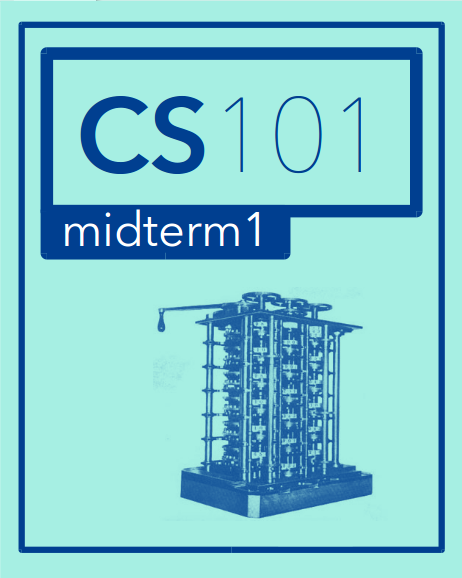
\includegraphics[width=2in]{../img/midterm1-header.png}
\end{center}

\bigskip
\noindent
\begin{itemize}
\item \textbf{Be sure to enter your \underline{NetID} and \underline{the code below} on your Scantron}.
\item Do not turn this page until instructed to do so.
\item There are 30 questions, worth 1 point each.
\item Each question has only \textbf{one} correct answer.
\item You must not communicate with other students during this test.
\item No books, notes, or electronic devices are permitted.
\item This is a 60-minute exam.
\item There are several different versions of this exam.
\end{itemize}

\bigskip\bigskip
\noindent
\textbf{\Large 1. Fill in your information:}

\bigskip
{\Large\bf
\begin{tabular}{ll}
Full Name: & \underbar{\hskip 8cm} \\[0.5em]
UIN (Student Number): & \underbar{\hskip 8cm} \\[0.5em]
NetID: & \underbar{\hskip 8cm}
\end{tabular}
}

\bigskip
\bigskip
\noindent
\textbf{\Large 2. Fill in the following answers on the Scantron form:}

%%%%%%%%%%%%%%%%%%%%%%%%%%%%%%%%%%%%%%%%%%%%%%%%%%%%%%%%%
%%%%%%%%%%%%%%%%%%%%%%%%%%%%%%%%%%%%%%%%%%%%%%%%%%%%%%%%%

\begin{enumerate}
\item[92.] D
\item[93.] B
\item[94.] B
\item[95.] D
\item[96.] A
\end{enumerate}

\newpage

% Zone 1


%%%%%%%%%%%%%%%%%%%%%%%%%%%%%%%%%%%%%%%%%%%%%%%%%%%%%%%%%



\newpage
\noindent
1. (1 point)
Consider the following program:
\begin{verbatim}
x=[1,2,3,4,5,6,7,8,9]
x=x[2:-2]
i=1
while i <= 3:
    x[i]+=1
    i+=1
\end{verbatim}
What is the \textbf{value} of \texttt{x} after this program is executed?


\begin{enumerate}
\item[(A)]
\begin{verbatim}[3, 5, 6, 7, 7, 8]\end{verbatim}

\item[(B)] $\bigstar$ 
\begin{verbatim}[3, 5, 6, 7, 7]\end{verbatim}

\item[(C)]
\begin{verbatim}[3, 5, 7, 7]\end{verbatim}

\item[(D)]
\begin{verbatim}[2, 4, 5, 5, 7, 7]\end{verbatim}

\item[(E)]
\begin{verbatim}[2, 4, 5, 6, 7, 7]\end{verbatim}

\end{enumerate}

\vspace*{2em}
\hrule
\vspace{2em}

\noindent {\bf Solution.} 
\vspace{2em}
\hrule height 2pt


\newpage
\noindent
2. (1 point)
Evaluate the following expression:
\begin{verbatim}
[1,2]*len("3")
\end{verbatim}
What value is produced?


\begin{enumerate}
\item[(A)]
\begin{verbatim}[1,2,1]\end{verbatim}

\item[(B)]
\begin{verbatim}[1,2,1,2,1,2]\end{verbatim}

\item[(C)] $\bigstar$ 
\begin{verbatim}[1,2]\end{verbatim}

\item[(D)]
\begin{verbatim}[1,2,3]\end{verbatim}

\end{enumerate}

\vspace*{2em}
\hrule
\vspace{2em}

\noindent {\bf Solution.} 
\vspace{2em}
\hrule height 2pt


\newpage
\noindent
3. (1 point)
Consider the following program.
\begin{verbatim}
s="ABCBA"
x=0
y=len(s)-1
while s[x]==s[y] and x<y:
    x+=1
    y-=1
\end{verbatim}
After it is run, what is the final \textbf{value} of \texttt{x}?


\begin{enumerate}
\item[(A)] $\bigstar$ 
\begin{verbatim}2\end{verbatim}

\item[(B)]
\begin{verbatim}1\end{verbatim}

\item[(C)]
\begin{verbatim}0\end{verbatim}

\item[(D)]
\begin{verbatim}3\end{verbatim}

\item[(E)]
\begin{verbatim}4\end{verbatim}

\end{enumerate}

\vspace*{2em}
\hrule
\vspace{2em}

\noindent {\bf Solution.} 
\vspace{2em}
\hrule height 2pt


\newpage
\noindent
4. (1 point)
Consider the following program:
\begin{verbatim}
s="ECTOR"
t="GAWAIN"
x=len(str(s.isupper()))-t.find("A")
\end{verbatim}
What is the \textbf{type} of \texttt{x} after this program is executed?


\begin{enumerate}
\item[(A)]
\begin{verbatim}Boolean\end{verbatim}

\item[(B)]
\begin{verbatim}None\end{verbatim}

\item[(C)]
\begin{verbatim}Float\end{verbatim}

\item[(D)] $\bigstar$ 
\begin{verbatim}Integer\end{verbatim}

\item[(E)]
\begin{verbatim}String\end{verbatim}

\end{enumerate}

\vspace*{2em}
\hrule
\vspace{2em}

\noindent {\bf Solution.} 
\vspace{2em}
\hrule height 2pt


\newpage
\noindent
5. (1 point)
Consider the following program:
\begin{verbatim}
x=str("1"*3)
\end{verbatim}
What is the \textbf{value} of \texttt{x} after this program is executed?


\begin{enumerate}
\item[(A)]
\begin{verbatim}"3"\end{verbatim}

\item[(B)] $\bigstar$ 
\begin{verbatim}"111"\end{verbatim}

\item[(C)]
\begin{verbatim}111\end{verbatim}

\item[(D)]
\begin{verbatim}3\end{verbatim}

\item[(E)]
None of the other answers are correct.

\end{enumerate}

\vspace*{2em}
\hrule
\vspace{2em}

\noindent {\bf Solution.} 
\vspace{2em}
\hrule height 2pt


\newpage
\noindent
6. (1 point)
Consider the following incomplete Python program.
\begin{verbatim}
s="".join(["1","0","2","1"])
x=0
for i in range(len(s)-1):
    x+=int(???)
\end{verbatim}
What should replace the three question marks so the resulting value of \texttt{x} is 33?


\begin{enumerate}
\item[(A)]
\begin{verbatim}s[i:i+1]\end{verbatim}

\item[(B)] $\bigstar$ 
\begin{verbatim}s[i:i+2]\end{verbatim}

\item[(C)]
\begin{verbatim}s[i:i-1]\end{verbatim}

\item[(D)]
\begin{verbatim}s[i+1:i+2]\end{verbatim}

\end{enumerate}

\vspace*{2em}
\hrule
\vspace{2em}

\noindent {\bf Solution.} 
\vspace{2em}
\hrule height 2pt


\newpage
\noindent
7. (1 point)
For this problem, you should compose a function which accomplishes a given task using the available code blocks arranged in the correct functional order.  \emph{We ignore indentation for this problem.}

\texttt{find\_max} should accept a \texttt{list} and return the value of the maximum item in the \texttt{list}.  (\texttt{None} is always the lowest value in any numeric comparison, so you may use it as an initializer.)

\begin{verbatim}
def find_max(my_list):
\end{verbatim}

\begin{enumerate}[1]
\item \texttt{max\_val = i}
\item \texttt{max\_val = None}
\item \texttt{for i in range(len(my\_list)):}
\item \texttt{if i > max\_val:}
\item \texttt{max\_val = my\_list[i]}
\item \texttt{return max\_val}
\item \texttt{for i in range(my\_list):}
\item \texttt{if my\_list[i] > max\_val:}
\item \texttt{print(max\_val)}
\end{enumerate}



\begin{enumerate}
\item[(A)]
3, 2, 8, 5, 9

\item[(B)] $\bigstar$ 
2, 3, 8, 5, 6

\item[(C)]
2, 3, 8, 1, 6

\item[(D)]
2, 7, 4, 5, 6

\item[(E)]
2, 3, 4, 1, 6

\end{enumerate}

\vspace*{2em}
\hrule
\vspace{2em}

\noindent {\bf Solution.} 
\vspace{2em}
\hrule height 2pt


\newpage
\noindent
8. (1 point)
How can the following mathematical equation be implemented as a Python expression? Assume \verb|a|, \verb|b|, and \verb|sin| have already been defined.
$$a \sin(a^b - b)$$


\begin{enumerate}
\item[(A)] $\bigstar$ 
\begin{verbatim}a*sin(a**b - b)\end{verbatim}

\item[(B)]
\begin{verbatim}a*sin(b^a - b)\end{verbatim}

\item[(C)]
\begin{verbatim}a*sin(a^b - b)\end{verbatim}

\item[(D)]
None of the other answers are correct.

\item[(E)]
\begin{verbatim}a sin(a**b - b)\end{verbatim}

\end{enumerate}

\vspace*{2em}
\hrule
\vspace{2em}

\noindent {\bf Solution.} 
\vspace{2em}
\hrule height 2pt


\newpage
\noindent
9. (1 point)
Consider the following program.
\begin{verbatim}
x=0
i=1
while(i*i)<=9:
    x=x+(i*i)
    i=i+1
\end{verbatim}
After it is run, what is the final \textbf{value} of \texttt{x}?


\begin{enumerate}
\item[(A)]
\begin{verbatim}3\end{verbatim}

\item[(B)]
\begin{verbatim}4\end{verbatim}

\item[(C)]
\begin{verbatim}5\end{verbatim}

\item[(D)]
\begin{verbatim}30\end{verbatim}

\item[(E)] $\bigstar$ 
\begin{verbatim}14\end{verbatim}

\end{enumerate}

\vspace*{2em}
\hrule
\vspace{2em}

\noindent {\bf Solution.} 
\vspace{2em}
\hrule height 2pt


\newpage
\noindent
10. (1 point)
Consider the following program:
\begin{verbatim}
s="TRIS %i"
t="ISEU"
x=s % len(t)
\end{verbatim}
What is the \textbf{type} of \texttt{x} after this program is executed?


\begin{enumerate}
\item[(A)]
\begin{verbatim}None\end{verbatim}

\item[(B)]
\begin{verbatim}Float\end{verbatim}

\item[(C)]
\begin{verbatim}Boolean\end{verbatim}

\item[(D)] $\bigstar$ 
\begin{verbatim}String\end{verbatim}

\item[(E)]
\begin{verbatim}Integer\end{verbatim}

\end{enumerate}

\vspace*{2em}
\hrule
\vspace{2em}

\noindent {\bf Solution.} 
\vspace{2em}
\hrule height 2pt


\newpage
\noindent
11. (1 point)
Consider the following program:
\begin{verbatim}
x=[1,2,3]
def f(a):
    s=""
    a.append(4)
    for i in a:
        s+=str(i)
    return s

x.append(f(x))
\end{verbatim}
What is the \textbf{value} of \texttt{x} after this program is executed?


\begin{enumerate}
\item[(A)]
\begin{verbatim}[1, 2, 3]\end{verbatim}

\item[(B)] $\bigstar$ 
\begin{verbatim}[1, 2, 3, 4, '1234']\end{verbatim}

\item[(C)]
\begin{verbatim}[1, 2, 3, '1234']\end{verbatim}

\item[(D)]
\begin{verbatim}[1, 2, 3, '123']\end{verbatim}

\item[(E)]
\begin{verbatim}[1, 2, 3, 10]\end{verbatim}

\end{enumerate}

\vspace*{2em}
\hrule
\vspace{2em}

\noindent {\bf Solution.} 
\vspace{2em}
\hrule height 2pt


\newpage
\noindent
12. (1 point)
Consider the following program:
\begin{verbatim}
s="G+R+A+I+L"
x=s.split("+")[1:-2]
\end{verbatim}
What is the \textbf{value} of \texttt{x} after this program is executed?


\begin{enumerate}
\item[(A)]
\begin{verbatim}'RAI'\end{verbatim}

\item[(B)] $\bigstar$ 
\begin{verbatim}['R','A']\end{verbatim}

\item[(C)]
\begin{verbatim}False\end{verbatim}

\item[(D)]
\begin{verbatim}None\end{verbatim}

\item[(E)]
\begin{verbatim}3\end{verbatim}

\end{enumerate}

\vspace*{2em}
\hrule
\vspace{2em}

\noindent {\bf Solution.} 
\vspace{2em}
\hrule height 2pt


\newpage
\noindent
13. (1 point)
What is the result of the following expression?
\begin{verbatim}
[ 1, 2, 3 ] * 3
\end{verbatim}


\begin{enumerate}
\item[(A)]
\begin{verbatim}(3, 6, 9)\end{verbatim}

\item[(B)]
\begin{verbatim}[1.0, 2.0, 3.0, 1.0, 2.0, 3.0, 1.0, 2.0, 3.0]\end{verbatim}

\item[(C)] $\bigstar$ 
\begin{verbatim}[1, 2, 3, 1, 2, 3, 1, 2, 3]\end{verbatim}

\item[(D)]
\begin{verbatim}[3.0, 6.0, 9.0]\end{verbatim}

\item[(E)]
\begin{verbatim}[3, 6, 9]\end{verbatim}

\end{enumerate}

\vspace*{2em}
\hrule
\vspace{2em}

\noindent {\bf Solution.} 
\vspace{2em}
\hrule height 2pt


\newpage
\noindent
14. (1 point)
Consider the following program:
\begin{verbatim}
a=3
b=4
if a==3:
    a=b
elif a==4:
    a=5
else:
    b=a
\end{verbatim}
What is the \textbf{value} of a after this program is executed?


\begin{enumerate}
\item[(A)]
\begin{verbatim}3\end{verbatim}

\item[(B)] $\bigstar$ 
\begin{verbatim}4\end{verbatim}

\item[(C)]
\begin{verbatim}7\end{verbatim}

\item[(D)]
\begin{verbatim}5\end{verbatim}

\item[(E)]
None of the other answers are correct.

\end{enumerate}

\vspace*{2em}
\hrule
\vspace{2em}

\noindent {\bf Solution.} 
\vspace{2em}
\hrule height 2pt


\newpage
\noindent
15. (1 point)
Consider the following program:
\begin{verbatim}
pi="3.14159"
e="2.71828"
x=pi in pi*len(e)
\end{verbatim}
What is the \textbf{type} of \texttt{x} after this program is executed?


\begin{enumerate}
\item[(A)]
\begin{verbatim}None\end{verbatim}

\item[(B)]
\begin{verbatim}String\end{verbatim}

\item[(C)] $\bigstar$ 
\begin{verbatim}Boolean\end{verbatim}

\item[(D)]
\begin{verbatim}Integer\end{verbatim}

\item[(E)]
\begin{verbatim}Float\end{verbatim}

\end{enumerate}

\vspace*{2em}
\hrule
\vspace{2em}

\noindent {\bf Solution.} 
\vspace{2em}
\hrule height 2pt


\newpage
\noindent
16. (1 point)
Consider the following incomplete program.
\begin{verbatim}
sum=0
for i in range(0,100):
    ???

\end{verbatim}
The program is intended to sum all of the integers between 1 and 100 (inclusive). What should replace the three question marks to complete the program?


\begin{enumerate}
\item[(A)]
\begin{verbatim}sum+1=sum \end{verbatim}

\item[(B)] $\bigstar$ 
\begin{verbatim}sum=sum+i+1 \end{verbatim}

\item[(C)]
\begin{verbatim}sum=sum+i \end{verbatim}

\item[(D)]
\begin{verbatim}sum=sum+1\end{verbatim}

\end{enumerate}

\vspace*{2em}
\hrule
\vspace{2em}

\noindent {\bf Solution.} 
\vspace{2em}
\hrule height 2pt


\newpage
\noindent
17. (1 point)
Consider the following program:
\begin{verbatim}
i=3
x=2
while i < 7:
    x+=i
    i+=2
\end{verbatim}
What is the \textbf{value} of \texttt{x} after this program is executed?


\begin{enumerate}
\item[(A)] $\bigstar$ 
\begin{verbatim}10\end{verbatim}

\item[(B)]
\begin{verbatim}12\end{verbatim}

\item[(C)]
\begin{verbatim}14\end{verbatim}

\item[(D)]
\begin{verbatim}13\end{verbatim}

\item[(E)]
\begin{verbatim}11\end{verbatim}

\end{enumerate}

\vspace*{2em}
\hrule
\vspace{2em}

\noindent {\bf Solution.} 
\vspace{2em}
\hrule height 2pt


\newpage
\noindent
18. (1 point)
Consider the following program:
\begin{verbatim}
a=["S","T","U","P","E","F","Y"]
a=a[0:4]
a.sort()
x=""
for e in a:
    x=e+x
\end{verbatim}
What is the \textbf{value} of \texttt{x} after this program is executed?


\begin{enumerate}
\item[(A)]
None of the other answers are correct.

\item[(B)]
\begin{verbatim}"STUP"\end{verbatim}

\item[(C)]
\begin{verbatim}"PSTU"\end{verbatim}

\item[(D)] $\bigstar$ 
\begin{verbatim}"UTSP"\end{verbatim}

\item[(E)]
\begin{verbatim}"PUST"\end{verbatim}

\end{enumerate}

\vspace*{2em}
\hrule
\vspace{2em}

\noindent {\bf Solution.} 
\vspace{2em}
\hrule height 2pt


\newpage
\noindent
19. (1 point)
Consider the following program.
\begin{verbatim}
x=[]
for j in range(0,5):
    if (j%2)==0:
        x.append("-")
    if (j%5)==0:
        x.append("*")
\end{verbatim}
After it is run, what is the final \textbf{value} of \texttt{x}?


\begin{enumerate}
\item[(A)]
\begin{verbatim}["*","-","*","*"]\end{verbatim}

\item[(B)]
\begin{verbatim}["-","*","-"]\end{verbatim}

\item[(C)]
None of the other answers are correct.

\item[(D)] $\bigstar$ 
\begin{verbatim}["-","*","-","-"]\end{verbatim}

\item[(E)]
\begin{verbatim}["-","-","*"]\end{verbatim}

\end{enumerate}

\vspace*{2em}
\hrule
\vspace{2em}

\noindent {\bf Solution.} 
\vspace{2em}
\hrule height 2pt


\newpage
\noindent
20. (1 point)
Evaluate the following expression:
\begin{verbatim}
len("ABCD"[0:3])
\end{verbatim}
What value is produced?


\begin{enumerate}
\item[(A)]
4

\item[(B)] $\bigstar$ 
3

\item[(C)]
1

\item[(D)]
2

\end{enumerate}

\vspace*{2em}
\hrule
\vspace{2em}

\noindent {\bf Solution.} 
\vspace{2em}
\hrule height 2pt


\newpage
\noindent
21. (1 point)
Consider the following program.
\begin{verbatim}
kay = 2
wart = 3

def knight(kay,wart):
    wart += 2
    kay += 3
    return wart + kay

wart = knight(kay, kay) + knight(wart, wart)
\end{verbatim}
After it is run, what is the final \textbf{value} of \texttt{wart}?


\begin{enumerate}
\item[(A)] $\bigstar$ 
None of the other answers are correct.

\item[(B)]
\begin{verbatim}3\end{verbatim}

\item[(C)]
\begin{verbatim}5\end{verbatim}

\item[(D)]
\begin{verbatim}2\end{verbatim}

\end{enumerate}

\vspace*{2em}
\hrule
\vspace{2em}

\noindent {\bf Solution.} 
\vspace{2em}
\hrule height 2pt


\newpage
\noindent
22. (1 point)
Consider the following program:
\begin{verbatim}
x=2
a=6
if (a%3)==2:
    x=x**3
elif(a%3)==1:
    x=x**2
else:
    x=x**1
\end{verbatim}
What is the \textbf{value} of \texttt{x} after this program is executed?


\begin{enumerate}
\item[(A)]
\begin{verbatim}4\end{verbatim}

\item[(B)] $\bigstar$ 
\begin{verbatim}2\end{verbatim}

\item[(C)]
None of the other answers are correct.

\item[(D)]
\begin{verbatim}8\end{verbatim}

\item[(E)]
\begin{verbatim}16\end{verbatim}

\end{enumerate}

\vspace*{2em}
\hrule
\vspace{2em}

\noindent {\bf Solution.} 
\vspace{2em}
\hrule height 2pt


\newpage
\noindent
23. (1 point)
Consider the following incomplete function.
\begin{verbatim}
def ismultiple(m,n):
    if ???:
        return False
    else:
        return True
\end{verbatim}
The function is intended to return True if the input parameter m is a multiple of parameter n and False otherwise. For example, \verb|ismultiple(4,2)| should return \verb|True|, but \verb|ismultiple(5,3)| should return \verb|False|. What should replace the three question marks to complete the function?


\begin{enumerate}
\item[(A)] $\bigstar$ 
\begin{verbatim}(m % n) != 0 \end{verbatim}

\item[(B)]
\begin{verbatim}(m // n) != 0 \end{verbatim}

\item[(C)]
\begin{verbatim}(n % m) == 0 \end{verbatim}

\item[(D)]
\begin{verbatim}(n // m) == 0 \end{verbatim}

\end{enumerate}

\vspace*{2em}
\hrule
\vspace{2em}

\noindent {\bf Solution.} 
\vspace{2em}
\hrule height 2pt


\newpage
\noindent
24. (1 point)
Consider the following program:
\begin{verbatim}
x=0
for i in range(2,7):
    if i%3==0:
        x+=3
    elif i%2==0:
        x+=2
    else:
        x+=1
\end{verbatim}
What is the \textbf{value} of \texttt{x} after this program is executed?


\begin{enumerate}
\item[(A)] $\bigstar$ 
\begin{verbatim}11\end{verbatim}

\item[(B)]
\begin{verbatim}12\end{verbatim}

\item[(C)]
\begin{verbatim}14\end{verbatim}

\item[(D)]
\begin{verbatim}13\end{verbatim}

\item[(E)]
\begin{verbatim}10\end{verbatim}

\end{enumerate}

\vspace*{2em}
\hrule
\vspace{2em}

\noindent {\bf Solution.} 
\vspace{2em}
\hrule height 2pt


\newpage
\noindent
25. (1 point)
Consider the following program.
\begin{verbatim}
def artificing(s):
    return s*2
    return s+"%i" % 2
    return s

s=artificing("MERLIN")
\end{verbatim}
After it is run, what is the final \textbf{value} of s?


\begin{enumerate}
\item[(A)]
\begin{verbatim}None\end{verbatim}

\item[(B)] $\bigstar$ 
\begin{verbatim}"MERLINMERLIN"\end{verbatim}

\item[(C)]
\begin{verbatim}"MERLIN2"\end{verbatim}

\item[(D)]
\begin{verbatim}"MERLIN"\end{verbatim}

\item[(E)]
\begin{verbatim}12\end{verbatim}

\end{enumerate}

\vspace*{2em}
\hrule
\vspace{2em}

\noindent {\bf Solution.} 
\vspace{2em}
\hrule height 2pt


\newpage
\noindent
26. (1 point)
Consider the following Python program.
\begin{verbatim}
e=[1,3,5,7,9,11]
d=[0,0,0]
for i in range(0,len(e)):
    d[i%3]+=e[i]
x=d[1]
\end{verbatim}
After it is run, what is the final \textbf{value} of \texttt{x}?


\begin{enumerate}
\item[(A)] $\bigstar$ 
\begin{verbatim}12\end{verbatim}

\item[(B)]
\begin{verbatim}3\end{verbatim}

\item[(C)]
\begin{verbatim}16\end{verbatim}

\item[(D)]
\begin{verbatim}8\end{verbatim}

\item[(E)]
\begin{verbatim}0\end{verbatim}

\end{enumerate}

\vspace*{2em}
\hrule
\vspace{2em}

\noindent {\bf Solution.} 
\vspace{2em}
\hrule height 2pt


\newpage
\noindent
27. (1 point)
Consider the following program:
\begin{verbatim}
x="KING ARTHUR-MORGANA LEFAY-SIR BEDIVERE".split("-")
y=x
y.reverse()
\end{verbatim}
What is the \textbf{value} of \texttt{x} after this program is executed?


\begin{enumerate}
\item[(A)]
\begin{verbatim}['KING ARTHUR', 'MORGANA LEFAY', 'SIR BEDIVERE']\end{verbatim}

\item[(B)]
\begin{verbatim}None\end{verbatim}

\item[(C)]
\begin{verbatim}['KING', 'ARTHUR-MORGANA', 'LEFAY-SIR', 'BEDIVERE']\end{verbatim}

\item[(D)] $\bigstar$ 
\begin{verbatim}['SIR BEDIVERE', 'MORGANA LEFAY', 'KING ARTHUR']\end{verbatim}

\item[(E)]
\begin{verbatim}['BEDIVERE', 'LEFAY-SIR', 'ARTHUR-MORGANA', 'KING']\end{verbatim}

\end{enumerate}

\vspace*{2em}
\hrule
\vspace{2em}

\noindent {\bf Solution.} 
\vspace{2em}
\hrule height 2pt


\newpage
\noindent
28. (1 point)
Consider the following program:
\begin{verbatim}
s="Hobbes"
i=0
x=-1
while i<len(s):
    if s[i]=='b':
        x=i
    i+=1
\end{verbatim}
What is the \textbf{value} of \texttt{x} after this program is executed?


\begin{enumerate}
\item[(A)]
\begin{verbatim}2\end{verbatim}

\item[(B)]
\begin{verbatim}4\end{verbatim}

\item[(C)]
\begin{verbatim}-1\end{verbatim}

\item[(D)] $\bigstar$ 
\begin{verbatim}3\end{verbatim}

\item[(E)]
\begin{verbatim}5\end{verbatim}

\end{enumerate}

\vspace*{2em}
\hrule
\vspace{2em}

\noindent {\bf Solution.} 
\vspace{2em}
\hrule height 2pt


\newpage
\noindent
29. (1 point)
Consider the following program:
\begin{verbatim}
def fix(s):
    a=list(s)
    a.sort()
    return ''.join(a)

x=["one","two","eleven","twelve"]
s1=fix(x[0]+x[-1])
s2=fix(x[1]+x[-2])

if s1<s2:
    x.sort()
elif s1>s2:
    x.reverse()
else:
    x.append("six")
\end{verbatim}
What is the \textbf{value} of \texttt{x} after this program is executed?


\begin{enumerate}
\item[(A)] $\bigstar$ 
\begin{verbatim}['one', 'two', 'eleven', 'twelve', 'six']\end{verbatim}

\item[(B)]
\begin{verbatim}['one', 'two', 'eleven', 'twelve']\end{verbatim}

\item[(C)]
\begin{verbatim}['eleven', 'one', 'twelve', 'two']\end{verbatim}

\item[(D)]
\begin{verbatim}['twelve', 'eleven', 'two', 'one']\end{verbatim}

\item[(E)]
\begin{verbatim}['two', 'twelve', 'one', 'eleven', 'six']\end{verbatim}

\end{enumerate}

\vspace*{2em}
\hrule
\vspace{2em}

\noindent {\bf Solution.} 
\vspace{2em}
\hrule height 2pt


\newpage
\noindent
30. (1 point)
Consider the following program:
\begin{verbatim}
a=["merlin","sir agravaine","king pellinore"]
b=[ ]
for i in range(0,3):
    b.append(a[0-i].title())
\end{verbatim}
What is the \textbf{value} of b after this program is executed?


\begin{enumerate}
\item[(A)]
\begin{verbatim}['King Pellinore', 'Sir Agravaine', 'Merlin']\end{verbatim}

\item[(B)]
\begin{verbatim}['King Pellinore', 'Sir Agravaine']\end{verbatim}

\item[(C)]
\begin{verbatim}[ ]\end{verbatim}

\item[(D)]
\begin{verbatim}['Sir Agravaine', 'King Pellinore']\end{verbatim}

\item[(E)] $\bigstar$ 
\begin{verbatim}['Merlin', 'King Pellinore', 'Sir Agravaine']\end{verbatim}

\end{enumerate}

\vspace*{2em}
\hrule
\vspace{2em}

\noindent {\bf Solution.} 
\vspace{2em}
\hrule height 2pt

%%%%%%%%%%%%%%%%%%%%%%%%%%%%%%%%%%%%%%%%%%%%%%%%%%%%%%%%%%%%%%%%%%%%%%
%%%%%%%%%%%%%%%%%%%%%%%%%%%%%%%%%%%%%%%%%%%%%%%%%%%%%%%%%%%%%%%%%%%%%%
%%%%%%%%%%%%%%%%%%%%%%%%%%%%%%%%%%%%%%%%%%%%%%%%%%%%%%%%%%%%%%%%%%%%%%
%%%%%%%%%%%%%%%%%%%%%%%%%%%%%%%%%%%%%%%%%%%%%%%%%%%%%%%%%%%%%%%%%%%%%%
% Exam number 35

\message{Exam 35/50}
\cleardoublepage
\setcounter{page}{1}


\begin{center}
%\textbf{\Large CS 101 Midterm \#1}
%
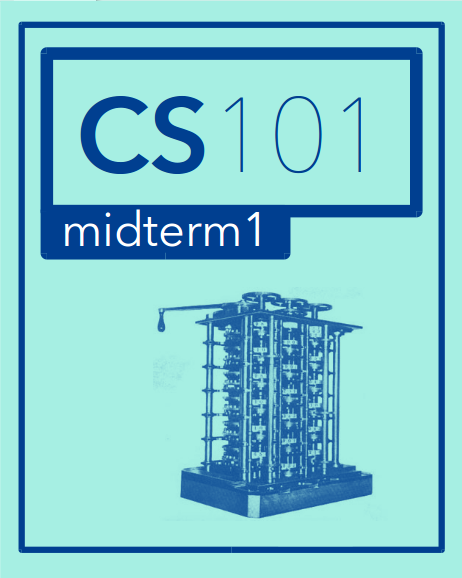
\includegraphics[width=2in]{../img/midterm1-header.png}
\end{center}

\bigskip
\noindent
\begin{itemize}
\item \textbf{Be sure to enter your \underline{NetID} and \underline{the code below} on your Scantron}.
\item Do not turn this page until instructed to do so.
\item There are 30 questions, worth 1 point each.
\item Each question has only \textbf{one} correct answer.
\item You must not communicate with other students during this test.
\item No books, notes, or electronic devices are permitted.
\item This is a 60-minute exam.
\item There are several different versions of this exam.
\end{itemize}

\bigskip\bigskip
\noindent
\textbf{\Large 1. Fill in your information:}

\bigskip
{\Large\bf
\begin{tabular}{ll}
Full Name: & \underbar{\hskip 8cm} \\[0.5em]
UIN (Student Number): & \underbar{\hskip 8cm} \\[0.5em]
NetID: & \underbar{\hskip 8cm}
\end{tabular}
}

\bigskip
\bigskip
\noindent
\textbf{\Large 2. Fill in the following answers on the Scantron form:}

%%%%%%%%%%%%%%%%%%%%%%%%%%%%%%%%%%%%%%%%%%%%%%%%%%%%%%%%%
%%%%%%%%%%%%%%%%%%%%%%%%%%%%%%%%%%%%%%%%%%%%%%%%%%%%%%%%%

\begin{enumerate}
\item[92.] E
\item[93.] B
\item[94.] B
\item[95.] E
\item[96.] B
\end{enumerate}

\newpage

% Zone 1


%%%%%%%%%%%%%%%%%%%%%%%%%%%%%%%%%%%%%%%%%%%%%%%%%%%%%%%%%



\newpage
\noindent
1. (1 point)
What is the result of the following expression?
\begin{verbatim}
[ 1, 2, 3 ] * 3
\end{verbatim}


\begin{enumerate}
\item[(A)]
\begin{verbatim}(3, 6, 9)\end{verbatim}

\item[(B)]
\begin{verbatim}[3.0, 6.0, 9.0]\end{verbatim}

\item[(C)] $\bigstar$ 
\begin{verbatim}[1, 2, 3, 1, 2, 3, 1, 2, 3]\end{verbatim}

\item[(D)]
\begin{verbatim}[1.0, 2.0, 3.0, 1.0, 2.0, 3.0, 1.0, 2.0, 3.0]\end{verbatim}

\item[(E)]
\begin{verbatim}[3, 6, 9]\end{verbatim}

\end{enumerate}

\vspace*{2em}
\hrule
\vspace{2em}

\noindent {\bf Solution.} 
\vspace{2em}
\hrule height 2pt


\newpage
\noindent
2. (1 point)
Consider the following Python program.
\begin{verbatim}
e=[1,3,5,7,9,11]
d=[0,0,0]
for i in range(0,len(e)):
    d[i%3]+=e[i]
x=d[2]
\end{verbatim}
After it is run, what is the final \textbf{value} of \texttt{x}?


\begin{enumerate}
\item[(A)]
\begin{verbatim}0\end{verbatim}

\item[(B)] $\bigstar$ 
\begin{verbatim}16\end{verbatim}

\item[(C)]
\begin{verbatim}8\end{verbatim}

\item[(D)]
\begin{verbatim}7\end{verbatim}

\item[(E)]
\begin{verbatim}12\end{verbatim}

\end{enumerate}

\vspace*{2em}
\hrule
\vspace{2em}

\noindent {\bf Solution.} 
\vspace{2em}
\hrule height 2pt


\newpage
\noindent
3. (1 point)
Consider the following program:
\begin{verbatim}
x="KING ARTHUR-MORGANA LEFAY-SIR BEDIVERE".split("-")
y=x
x=y.reverse()
\end{verbatim}
What is the \textbf{value} of \texttt{x} after this program is executed?


\begin{enumerate}
\item[(A)]
\begin{verbatim}['KING ARTHUR', 'MORGANA LEFAY', 'SIR BEDIVERE']\end{verbatim}

\item[(B)]
\begin{verbatim}['KING', 'ARTHUR-MORGANA', 'LEFAY-SIR', 'BEDIVERE']\end{verbatim}

\item[(C)]
\begin{verbatim}['BEDIVERE', 'LEFAY-SIR', 'ARTHUR-MORGANA', 'KING']\end{verbatim}

\item[(D)]
\begin{verbatim}['SIR BEDIVERE', 'MORGANA LEFAY', 'KING ARTHUR']\end{verbatim}

\item[(E)] $\bigstar$ 
\begin{verbatim}None\end{verbatim}

\end{enumerate}

\vspace*{2em}
\hrule
\vspace{2em}

\noindent {\bf Solution.} 
\vspace{2em}
\hrule height 2pt


\newpage
\noindent
4. (1 point)
Evaluate the following expression:
\begin{verbatim}
[1,2]+[len("3")]
\end{verbatim}
What value is produced?


\begin{enumerate}
\item[(A)]
\begin{verbatim}[1,2,"3"]\end{verbatim}

\item[(B)]
\begin{verbatim}[1,2,3]\end{verbatim}

\item[(C)] $\bigstar$ 
\begin{verbatim}[1,2,1]\end{verbatim}

\item[(D)]
\begin{verbatim}[1,2,1,2,1,2]\end{verbatim}

\end{enumerate}

\vspace*{2em}
\hrule
\vspace{2em}

\noindent {\bf Solution.} 
\vspace{2em}
\hrule height 2pt


\newpage
\noindent
5. (1 point)
Consider the following program:
\begin{verbatim}
a=["A","C","C","I","O"]
a.sort()
a[0]=a[-1]
x=""
for e in a:
    x=x+e
\end{verbatim}
What is the \textbf{value} of \texttt{x} after this program is executed?


\begin{enumerate}
\item[(A)]
None of the other answers are correct.

\item[(B)]
\begin{verbatim}"ACCOA"\end{verbatim}

\item[(C)]
\begin{verbatim}"ICCOI"\end{verbatim}

\item[(D)]
\begin{verbatim}"ACCIA"\end{verbatim}

\item[(E)] $\bigstar$ 
\begin{verbatim}"OCCIO"\end{verbatim}

\end{enumerate}

\vspace*{2em}
\hrule
\vspace{2em}

\noindent {\bf Solution.} 
\vspace{2em}
\hrule height 2pt


\newpage
\noindent
6. (1 point)
Consider the following incomplete function.
\begin{verbatim}
def isdivisible(m,n):
    if ???:
        return False
    else:
        return True
\end{verbatim}
The function is intended to return True if the input parameter m is evenly divisible by the parameter n and False otherwise. For example, \verb|isdivisible(4,2)| should return \verb|True|, but \verb|isdivisible(5,3)| should return \verb|False|. What should replace the three question marks to complete the function?


\begin{enumerate}
\item[(A)] $\bigstar$ 
\begin{verbatim}(m % n) != 0 \end{verbatim}

\item[(B)]
\begin{verbatim}(n % m) == 0 \end{verbatim}

\item[(C)]
\begin{verbatim}(m // n) != 0 \end{verbatim}

\item[(D)]
\begin{verbatim}(n // m) == 0 \end{verbatim}

\end{enumerate}

\vspace*{2em}
\hrule
\vspace{2em}

\noindent {\bf Solution.} 
\vspace{2em}
\hrule height 2pt


\newpage
\noindent
7. (1 point)
Consider the following program.
\begin{verbatim}
x=[]
for j in range(0,5):
    if (j%4)==0:
        x.append("-")
    if (j%5)==0:
        x.append("*")
\end{verbatim}
After it is run, what is the final \textbf{value} of \texttt{x}?


\begin{enumerate}
\item[(A)]
\begin{verbatim}["-","-","*"]\end{verbatim}

\item[(B)]
\begin{verbatim}["-","*"]\end{verbatim}

\item[(C)]
None of the other answers are correct.

\item[(D)]
\begin{verbatim}["-","*","*"]\end{verbatim}

\item[(E)] $\bigstar$ 
\begin{verbatim}["-","*","-"]\end{verbatim}

\end{enumerate}

\vspace*{2em}
\hrule
\vspace{2em}

\noindent {\bf Solution.} 
\vspace{2em}
\hrule height 2pt


\newpage
\noindent
8. (1 point)
Consider the following program:
\begin{verbatim}
x=2
a=6
if (a%3)==2:
    x=x**3
elif(a%3)==1:
    x=x**2
else:
    x=x**1
\end{verbatim}
What is the \textbf{value} of \texttt{x} after this program is executed?


\begin{enumerate}
\item[(A)]
\begin{verbatim}4\end{verbatim}

\item[(B)]
\begin{verbatim}8\end{verbatim}

\item[(C)]
None of the other answers are correct.

\item[(D)]
\begin{verbatim}16\end{verbatim}

\item[(E)] $\bigstar$ 
\begin{verbatim}2\end{verbatim}

\end{enumerate}

\vspace*{2em}
\hrule
\vspace{2em}

\noindent {\bf Solution.} 
\vspace{2em}
\hrule height 2pt


\newpage
\noindent
9. (1 point)
Consider the following program:
\begin{verbatim}
x=[1,2,3,4,5,6,7,8,9]
x=x[2:-2]
i=1
while i <= 3:
    x[i]+=1
    i+=1
\end{verbatim}
What is the \textbf{value} of \texttt{x} after this program is executed?


\begin{enumerate}
\item[(A)]
\begin{verbatim}[2, 4, 5, 6, 7, 7]\end{verbatim}

\item[(B)] $\bigstar$ 
\begin{verbatim}[3, 5, 6, 7, 7]\end{verbatim}

\item[(C)]
\begin{verbatim}[3, 5, 6, 7, 7, 8]\end{verbatim}

\item[(D)]
\begin{verbatim}[2, 4, 5, 5, 7, 7]\end{verbatim}

\item[(E)]
\begin{verbatim}[3, 5, 7, 7]\end{verbatim}

\end{enumerate}

\vspace*{2em}
\hrule
\vspace{2em}

\noindent {\bf Solution.} 
\vspace{2em}
\hrule height 2pt


\newpage
\noindent
10. (1 point)
Consider the following program:
\begin{verbatim}
x=[1,2,3]
def f(a):
    s=""
    a.append(4)
    for i in a:
        s+=str(i)
    return s

x.append(f(x))
\end{verbatim}
What is the \textbf{value} of \texttt{x} after this program is executed?


\begin{enumerate}
\item[(A)] $\bigstar$ 
\begin{verbatim}[1, 2, 3, 4, '1234']\end{verbatim}

\item[(B)]
\begin{verbatim}[1, 2, 3, 10]\end{verbatim}

\item[(C)]
\begin{verbatim}[1, 2, 3, '1234']\end{verbatim}

\item[(D)]
\begin{verbatim}[1, 2, 3]\end{verbatim}

\item[(E)]
\begin{verbatim}[1, 2, 3, '123']\end{verbatim}

\end{enumerate}

\vspace*{2em}
\hrule
\vspace{2em}

\noindent {\bf Solution.} 
\vspace{2em}
\hrule height 2pt


\newpage
\noindent
11. (1 point)
Consider the following program:
\begin{verbatim}
def fix(s):
    a=list(s)
    a.sort()
    return ''.join(a)

x=["one","two","eleven","twelve"]
s1=fix(x[0]+x[-1])
s2=fix(x[1]+x[-2])

if s1<s2:
    x.sort()
elif s1==s2:
    x.reverse()
else:
    x.append("six")
\end{verbatim}
What is the \textbf{value} of \texttt{x} after this program is executed?


\begin{enumerate}
\item[(A)]
\begin{verbatim}['one', 'two', 'eleven', 'twelve']\end{verbatim}

\item[(B)]
\begin{verbatim}['eleven', 'one', 'twelve', 'two']\end{verbatim}

\item[(C)] $\bigstar$ 
\begin{verbatim}['twelve', 'eleven', 'two', 'one']\end{verbatim}

\item[(D)]
\begin{verbatim}['two', 'twelve', 'one', 'eleven', 'six']\end{verbatim}

\item[(E)]
\begin{verbatim}['one', 'two', 'eleven', 'twelve', 'six']\end{verbatim}

\end{enumerate}

\vspace*{2em}
\hrule
\vspace{2em}

\noindent {\bf Solution.} 
\vspace{2em}
\hrule height 2pt


\newpage
\noindent
12. (1 point)
Consider the following incomplete program.
\begin{verbatim}
sum=0
for i in range(0,100):
    ???

\end{verbatim}
The program is intended to sum all of the integers between 1 and 100 (inclusive). What should replace the three question marks to complete the program?


\begin{enumerate}
\item[(A)]
\begin{verbatim}sum=sum+1\end{verbatim}

\item[(B)]
\begin{verbatim}sum+1=sum \end{verbatim}

\item[(C)]
\begin{verbatim}sum=sum+i \end{verbatim}

\item[(D)] $\bigstar$ 
\begin{verbatim}sum=sum+i+1 \end{verbatim}

\end{enumerate}

\vspace*{2em}
\hrule
\vspace{2em}

\noindent {\bf Solution.} 
\vspace{2em}
\hrule height 2pt


\newpage
\noindent
13. (1 point)
Consider the following program:
\begin{verbatim}
s="Hobbes"
i=0
x=-1
while i<len(s):
    if s[i]=='b':
        x=i
    i+=1
\end{verbatim}
What is the \textbf{value} of \texttt{x} after this program is executed?


\begin{enumerate}
\item[(A)]
\begin{verbatim}2\end{verbatim}

\item[(B)]
\begin{verbatim}4\end{verbatim}

\item[(C)]
\begin{verbatim}5\end{verbatim}

\item[(D)]
\begin{verbatim}-1\end{verbatim}

\item[(E)] $\bigstar$ 
\begin{verbatim}3\end{verbatim}

\end{enumerate}

\vspace*{2em}
\hrule
\vspace{2em}

\noindent {\bf Solution.} 
\vspace{2em}
\hrule height 2pt


\newpage
\noindent
14. (1 point)
For this problem, you should compose a function which accomplishes a given task using the available code blocks arranged in the correct functional order.  \emph{We ignore indentation for this problem.}

\texttt{find\_max} should accept a \texttt{list} and return the value of the maximum item in the \texttt{list}.  (\texttt{None} is always the lowest value in any numeric comparison, so you may use it as an initializer.)

\begin{verbatim}
def find_max(my_list):
\end{verbatim}

\begin{enumerate}[1]
\item \texttt{max\_val = i}
\item \texttt{max\_val = None}
\item \texttt{for i in range(len(my\_list)):}
\item \texttt{if i > max\_val:}
\item \texttt{max\_val = my\_list[i]}
\item \texttt{return max\_val}
\item \texttt{for i in range(my\_list):}
\item \texttt{if my\_list[i] > max\_val:}
\item \texttt{print(max\_val)}
\end{enumerate}



\begin{enumerate}
\item[(A)] $\bigstar$ 
2, 3, 8, 5, 6

\item[(B)]
2, 3, 8, 1, 6

\item[(C)]
2, 7, 4, 5, 6

\item[(D)]
3, 2, 8, 5, 9

\item[(E)]
2, 3, 4, 1, 6

\end{enumerate}

\vspace*{2em}
\hrule
\vspace{2em}

\noindent {\bf Solution.} 
\vspace{2em}
\hrule height 2pt


\newpage
\noindent
15. (1 point)
Evaluate the following expression:
\begin{verbatim}
len("ABCD"[0:3])
\end{verbatim}
What value is produced?


\begin{enumerate}
\item[(A)] $\bigstar$ 
3

\item[(B)]
2

\item[(C)]
4

\item[(D)]
1

\end{enumerate}

\vspace*{2em}
\hrule
\vspace{2em}

\noindent {\bf Solution.} 
\vspace{2em}
\hrule height 2pt


\newpage
\noindent
16. (1 point)
Consider the following program:
\begin{verbatim}
s="ECTOR"
t="GAWAIN"
x=(len(s)+len(t)) < 4 and s in t
\end{verbatim}
What is the \textbf{type} of \texttt{x} after this program is executed?


\begin{enumerate}
\item[(A)]
\begin{verbatim}None\end{verbatim}

\item[(B)] $\bigstar$ 
\begin{verbatim}Boolean\end{verbatim}

\item[(C)]
\begin{verbatim}Integer\end{verbatim}

\item[(D)]
\begin{verbatim}String\end{verbatim}

\item[(E)]
\begin{verbatim}Float\end{verbatim}

\end{enumerate}

\vspace*{2em}
\hrule
\vspace{2em}

\noindent {\bf Solution.} 
\vspace{2em}
\hrule height 2pt


\newpage
\noindent
17. (1 point)
Consider the following program:
\begin{verbatim}
a=3
b=4
if a==3:
    a=b
elif a==4:
    a=5
else:
    b=a
\end{verbatim}
What is the \textbf{value} of a after this program is executed?


\begin{enumerate}
\item[(A)]
\begin{verbatim}5\end{verbatim}

\item[(B)]
None of the other answers are correct.

\item[(C)]
\begin{verbatim}7\end{verbatim}

\item[(D)] $\bigstar$ 
\begin{verbatim}4\end{verbatim}

\item[(E)]
\begin{verbatim}3\end{verbatim}

\end{enumerate}

\vspace*{2em}
\hrule
\vspace{2em}

\noindent {\bf Solution.} 
\vspace{2em}
\hrule height 2pt


\newpage
\noindent
18. (1 point)
Consider the following program:
\begin{verbatim}
a=["merlin","sir agravaine","king pellinore"]
b=[ ]
for i in range(1,3):
    b.append(a[0-i].title())
\end{verbatim}
What is the \textbf{value} of b after this program is executed?


\begin{enumerate}
\item[(A)]
\begin{verbatim}['Sir Agravaine', 'King Pellinore']\end{verbatim}

\item[(B)] $\bigstar$ 
\begin{verbatim}['King Pellinore', 'Sir Agravaine']\end{verbatim}

\item[(C)]
\begin{verbatim}['Merlin', 'King Pellinore', 'Sir Agravaine']\end{verbatim}

\item[(D)]
\begin{verbatim}['King Pellinore', 'Sir Agravaine', 'Merlin']\end{verbatim}

\item[(E)]
\begin{verbatim}[ ]\end{verbatim}

\end{enumerate}

\vspace*{2em}
\hrule
\vspace{2em}

\noindent {\bf Solution.} 
\vspace{2em}
\hrule height 2pt


\newpage
\noindent
19. (1 point)
Consider the following program.
\begin{verbatim}
kay = 2
wart = 3

def knight(kay,wart):
    wart += 2
    kay += 3
    return wart + kay

wart = knight(kay, kay) + knight(wart, wart)
\end{verbatim}
After it is run, what is the final \textbf{value} of \texttt{wart}?


\begin{enumerate}
\item[(A)] $\bigstar$ 
None of the other answers are correct.

\item[(B)]
\begin{verbatim}2\end{verbatim}

\item[(C)]
\begin{verbatim}5\end{verbatim}

\item[(D)]
\begin{verbatim}3\end{verbatim}

\end{enumerate}

\vspace*{2em}
\hrule
\vspace{2em}

\noindent {\bf Solution.} 
\vspace{2em}
\hrule height 2pt


\newpage
\noindent
20. (1 point)
Consider the following program:
\begin{verbatim}
s="-B-O-R-S-"
x=s.split("-")[2:-2]
\end{verbatim}
What is the \textbf{value} of \texttt{x} after this program is executed?


\begin{enumerate}
\item[(A)]
\begin{verbatim}False\end{verbatim}

\item[(B)]
\begin{verbatim}None\end{verbatim}

\item[(C)]
\begin{verbatim}'ORS'\end{verbatim}

\item[(D)]
\begin{verbatim}''\end{verbatim}

\item[(E)] $\bigstar$ 
\begin{verbatim}['O', 'R']\end{verbatim}

\end{enumerate}

\vspace*{2em}
\hrule
\vspace{2em}

\noindent {\bf Solution.} 
\vspace{2em}
\hrule height 2pt


\newpage
\noindent
21. (1 point)
How can the following mathematical equation be implemented as a Python expression? Assume \verb|a|, \verb|b|, and \verb|cos| have already been defined.
$$a^b \cos(a - b)$$


\begin{enumerate}
\item[(A)]
\begin{verbatim}(b^a)cos(a-b)\end{verbatim}

\item[(B)]
\begin{verbatim}(a**b)cos(a-b)\end{verbatim}

\item[(C)]
None of the other answers are correct.

\item[(D)]
\begin{verbatim}(a^b)*cos(a-b)\end{verbatim}

\item[(E)] $\bigstar$ 
\begin{verbatim}(a**b)*cos(a-b)\end{verbatim}

\end{enumerate}

\vspace*{2em}
\hrule
\vspace{2em}

\noindent {\bf Solution.} 
\vspace{2em}
\hrule height 2pt


\newpage
\noindent
22. (1 point)
Consider the following program:
\begin{verbatim}
x=str(1.2)*2
\end{verbatim}
What is the \textbf{value} of \texttt{x} after this program is executed?


\begin{enumerate}
\item[(A)] $\bigstar$ 
\begin{verbatim}"1.21.2"\end{verbatim}

\item[(B)]
\begin{verbatim}2.4\end{verbatim}

\item[(C)]
None of the other answers are correct.

\item[(D)]
\begin{verbatim}"1.2*2"\end{verbatim}

\item[(E)]
\begin{verbatim}"2.4"\end{verbatim}

\end{enumerate}

\vspace*{2em}
\hrule
\vspace{2em}

\noindent {\bf Solution.} 
\vspace{2em}
\hrule height 2pt


\newpage
\noindent
23. (1 point)
Consider the following program:
\begin{verbatim}
i=3
x=2
while i < 7:
    x+=i
    i+=2
\end{verbatim}
What is the \textbf{value} of \texttt{x} after this program is executed?


\begin{enumerate}
\item[(A)]
\begin{verbatim}14\end{verbatim}

\item[(B)] $\bigstar$ 
\begin{verbatim}10\end{verbatim}

\item[(C)]
\begin{verbatim}11\end{verbatim}

\item[(D)]
\begin{verbatim}13\end{verbatim}

\item[(E)]
\begin{verbatim}12\end{verbatim}

\end{enumerate}

\vspace*{2em}
\hrule
\vspace{2em}

\noindent {\bf Solution.} 
\vspace{2em}
\hrule height 2pt


\newpage
\noindent
24. (1 point)
Consider the following program.
\begin{verbatim}
s="ABCBA"
x=0
y=len(s)-1
while s[x]==s[y] and x<=y:
    x+=1
    y-=1
\end{verbatim}
After it is run, what is the final \textbf{value} of \texttt{x}?


\begin{enumerate}
\item[(A)]
\begin{verbatim}0\end{verbatim}

\item[(B)] $\bigstar$ 
\begin{verbatim}3\end{verbatim}

\item[(C)]
\begin{verbatim}1\end{verbatim}

\item[(D)]
\begin{verbatim}2\end{verbatim}

\item[(E)]
\begin{verbatim}4\end{verbatim}

\end{enumerate}

\vspace*{2em}
\hrule
\vspace{2em}

\noindent {\bf Solution.} 
\vspace{2em}
\hrule height 2pt


\newpage
\noindent
25. (1 point)
Consider the following program:
\begin{verbatim}
s="TRIS %i"
t="ISEU"
x=len(s) % len(t[2:-1])
\end{verbatim}
What is the \textbf{type} of \texttt{x} after this program is executed?


\begin{enumerate}
\item[(A)]
\begin{verbatim}None\end{verbatim}

\item[(B)] $\bigstar$ 
\begin{verbatim}Integer\end{verbatim}

\item[(C)]
\begin{verbatim}Float\end{verbatim}

\item[(D)]
\begin{verbatim}Boolean\end{verbatim}

\item[(E)]
\begin{verbatim}String\end{verbatim}

\end{enumerate}

\vspace*{2em}
\hrule
\vspace{2em}

\noindent {\bf Solution.} 
\vspace{2em}
\hrule height 2pt


\newpage
\noindent
26. (1 point)
Consider the following program.
\begin{verbatim}
x=0
i=1
while(i*i)<=9:
    x=x+(i*i)
    i=i+1
\end{verbatim}
After it is run, what is the final \textbf{value} of \texttt{x}?


\begin{enumerate}
\item[(A)]
\begin{verbatim}4\end{verbatim}

\item[(B)] $\bigstar$ 
\begin{verbatim}14\end{verbatim}

\item[(C)]
\begin{verbatim}3\end{verbatim}

\item[(D)]
\begin{verbatim}5\end{verbatim}

\item[(E)]
\begin{verbatim}30\end{verbatim}

\end{enumerate}

\vspace*{2em}
\hrule
\vspace{2em}

\noindent {\bf Solution.} 
\vspace{2em}
\hrule height 2pt


\newpage
\noindent
27. (1 point)
Consider the following program:
\begin{verbatim}
x=0
for i in range(4,10):
    if i%3==0:
        x+=3
    elif i%2==0:
        x+=2
    else:
        x+=1
\end{verbatim}
What is the \textbf{value} of \texttt{x} after this program is executed?


\begin{enumerate}
\item[(A)] $\bigstar$ 
\begin{verbatim}12\end{verbatim}

\item[(B)]
\begin{verbatim}11\end{verbatim}

\item[(C)]
\begin{verbatim}13\end{verbatim}

\item[(D)]
\begin{verbatim}14\end{verbatim}

\item[(E)]
\begin{verbatim}10\end{verbatim}

\end{enumerate}

\vspace*{2em}
\hrule
\vspace{2em}

\noindent {\bf Solution.} 
\vspace{2em}
\hrule height 2pt


\newpage
\noindent
28. (1 point)
Consider the following program:
\begin{verbatim}
pi="3.14159"
e="2.71828"
x=pi in pi*len(e)
\end{verbatim}
What is the \textbf{type} of \texttt{x} after this program is executed?


\begin{enumerate}
\item[(A)]
\begin{verbatim}Float\end{verbatim}

\item[(B)]
\begin{verbatim}None\end{verbatim}

\item[(C)]
\begin{verbatim}String\end{verbatim}

\item[(D)]
\begin{verbatim}Integer\end{verbatim}

\item[(E)] $\bigstar$ 
\begin{verbatim}Boolean\end{verbatim}

\end{enumerate}

\vspace*{2em}
\hrule
\vspace{2em}

\noindent {\bf Solution.} 
\vspace{2em}
\hrule height 2pt


\newpage
\noindent
29. (1 point)
Consider the following incomplete Python program.
\begin{verbatim}
s="".join(["2","2","0","1"])
x=0
for i in range(len(s)-1):
    x+=int(???)
\end{verbatim}
What should replace the three question marks so the resulting value of \texttt{x} is 43?


\begin{enumerate}
\item[(A)]
\begin{verbatim}s[i+1:i+2]\end{verbatim}

\item[(B)]
\begin{verbatim}s[i:i-1]\end{verbatim}

\item[(C)]
\begin{verbatim}s[i:i+1]\end{verbatim}

\item[(D)] $\bigstar$ 
\begin{verbatim}s[i:i+2]\end{verbatim}

\end{enumerate}

\vspace*{2em}
\hrule
\vspace{2em}

\noindent {\bf Solution.} 
\vspace{2em}
\hrule height 2pt


\newpage
\noindent
30. (1 point)
Consider the following program.
\begin{verbatim}
def artificing(s):
    return s*2
    return s+"%i" % 2
    return s

s=artificing("MERLIN")
\end{verbatim}
After it is run, what is the final \textbf{value} of s?


\begin{enumerate}
\item[(A)]
\begin{verbatim}"MERLIN"\end{verbatim}

\item[(B)]
\begin{verbatim}12\end{verbatim}

\item[(C)] $\bigstar$ 
\begin{verbatim}"MERLINMERLIN"\end{verbatim}

\item[(D)]
\begin{verbatim}None\end{verbatim}

\item[(E)]
\begin{verbatim}"MERLIN2"\end{verbatim}

\end{enumerate}

\vspace*{2em}
\hrule
\vspace{2em}

\noindent {\bf Solution.} 
\vspace{2em}
\hrule height 2pt

%%%%%%%%%%%%%%%%%%%%%%%%%%%%%%%%%%%%%%%%%%%%%%%%%%%%%%%%%%%%%%%%%%%%%%
%%%%%%%%%%%%%%%%%%%%%%%%%%%%%%%%%%%%%%%%%%%%%%%%%%%%%%%%%%%%%%%%%%%%%%
%%%%%%%%%%%%%%%%%%%%%%%%%%%%%%%%%%%%%%%%%%%%%%%%%%%%%%%%%%%%%%%%%%%%%%
%%%%%%%%%%%%%%%%%%%%%%%%%%%%%%%%%%%%%%%%%%%%%%%%%%%%%%%%%%%%%%%%%%%%%%
% Exam number 36

\message{Exam 36/50}
\cleardoublepage
\setcounter{page}{1}


\begin{center}
%\textbf{\Large CS 101 Midterm \#1}
%
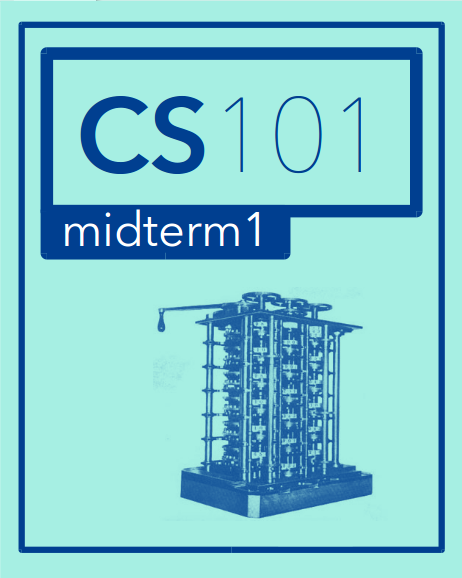
\includegraphics[width=2in]{../img/midterm1-header.png}
\end{center}

\bigskip
\noindent
\begin{itemize}
\item \textbf{Be sure to enter your \underline{NetID} and \underline{the code below} on your Scantron}.
\item Do not turn this page until instructed to do so.
\item There are 30 questions, worth 1 point each.
\item Each question has only \textbf{one} correct answer.
\item You must not communicate with other students during this test.
\item No books, notes, or electronic devices are permitted.
\item This is a 60-minute exam.
\item There are several different versions of this exam.
\end{itemize}

\bigskip\bigskip
\noindent
\textbf{\Large 1. Fill in your information:}

\bigskip
{\Large\bf
\begin{tabular}{ll}
Full Name: & \underbar{\hskip 8cm} \\[0.5em]
UIN (Student Number): & \underbar{\hskip 8cm} \\[0.5em]
NetID: & \underbar{\hskip 8cm}
\end{tabular}
}

\bigskip
\bigskip
\noindent
\textbf{\Large 2. Fill in the following answers on the Scantron form:}

%%%%%%%%%%%%%%%%%%%%%%%%%%%%%%%%%%%%%%%%%%%%%%%%%%%%%%%%%
%%%%%%%%%%%%%%%%%%%%%%%%%%%%%%%%%%%%%%%%%%%%%%%%%%%%%%%%%

\begin{enumerate}
\item[92.] A
\item[93.] C
\item[94.] B
\item[95.] B
\item[96.] E
\end{enumerate}

\newpage

% Zone 1


%%%%%%%%%%%%%%%%%%%%%%%%%%%%%%%%%%%%%%%%%%%%%%%%%%%%%%%%%



\newpage
\noindent
1. (1 point)
Consider the following program.
\begin{verbatim}
kay = 2
wart = 3

def knight(kay,wart):
    wart += 2
    kay += 3
    return wart + kay

wart = knight(kay, kay) + knight(wart, wart)
\end{verbatim}
After it is run, what is the final \textbf{value} of \texttt{wart}?


\begin{enumerate}
\item[(A)]
\begin{verbatim}3\end{verbatim}

\item[(B)]
\begin{verbatim}5\end{verbatim}

\item[(C)]
\begin{verbatim}2\end{verbatim}

\item[(D)] $\bigstar$ 
None of the other answers are correct.

\end{enumerate}

\vspace*{2em}
\hrule
\vspace{2em}

\noindent {\bf Solution.} 
\vspace{2em}
\hrule height 2pt


\newpage
\noindent
2. (1 point)
Consider the following incomplete program.
\begin{verbatim}
sum=0
???:
    sum=sum+i

\end{verbatim}
The program is intended to sum all of the integers between 1 and 100 (inclusive). What should replace the three question marks to complete the program?


\begin{enumerate}
\item[(A)]
\begin{verbatim}while i<=100 \end{verbatim}

\item[(B)] $\bigstar$ 
\begin{verbatim}for i in range(1,101) \end{verbatim}

\item[(C)]
\begin{verbatim}while i in range(100)\end{verbatim}

\item[(D)]
\begin{verbatim}for i in range(0,100)\end{verbatim}

\end{enumerate}

\vspace*{2em}
\hrule
\vspace{2em}

\noindent {\bf Solution.} 
\vspace{2em}
\hrule height 2pt


\newpage
\noindent
3. (1 point)
What is the result of the following expression?
\begin{verbatim}
[ 1, 2, 3 ] * 3.0
\end{verbatim}


\begin{enumerate}
\item[(A)]
\begin{verbatim}[3, 6, 9]\end{verbatim}

\item[(B)]
\begin{verbatim}[3.0, 6.0, 9.0]\end{verbatim}

\item[(C)]
\begin{verbatim}None of the above.\end{verbatim}

\item[(D)] $\bigstar$ 
\begin{verbatim}[1, 2, 3, 1, 2, 3, 1, 2, 3]\end{verbatim}

\item[(E)]
\begin{verbatim}[1.0, 2.0, 3.0, 1.0, 2.0, 3.0, 1.0, 2.0, 3.0]\end{verbatim}

\end{enumerate}

\vspace*{2em}
\hrule
\vspace{2em}

\noindent {\bf Solution.} 
\vspace{2em}
\hrule height 2pt


\newpage
\noindent
4. (1 point)
How can the following mathematical equation be implemented as a Python expression? Assume \verb|a|, \verb|b|, and \verb|sin| have already been defined.
$$a \sin(a^b - b)$$


\begin{enumerate}
\item[(A)] $\bigstar$ 
\begin{verbatim}a*sin(a**b - b)\end{verbatim}

\item[(B)]
\begin{verbatim}a*sin(a^b - b)\end{verbatim}

\item[(C)]
None of the other answers are correct.

\item[(D)]
\begin{verbatim}a sin(a**b - b)\end{verbatim}

\item[(E)]
\begin{verbatim}a*sin(b^a - b)\end{verbatim}

\end{enumerate}

\vspace*{2em}
\hrule
\vspace{2em}

\noindent {\bf Solution.} 
\vspace{2em}
\hrule height 2pt


\newpage
\noindent
5. (1 point)
Consider the following program:
\begin{verbatim}
s="ECTOR"
t="GAWAIN"
x=(len(s)/(len(t)-1))+1
\end{verbatim}
What is the \textbf{type} of \texttt{x} after this program is executed?


\begin{enumerate}
\item[(A)]
\begin{verbatim}Integer\end{verbatim}

\item[(B)] $\bigstar$ 
\begin{verbatim}Float\end{verbatim}

\item[(C)]
\begin{verbatim}String\end{verbatim}

\item[(D)]
\begin{verbatim}None\end{verbatim}

\item[(E)]
\begin{verbatim}Boolean\end{verbatim}

\end{enumerate}

\vspace*{2em}
\hrule
\vspace{2em}

\noindent {\bf Solution.} 
\vspace{2em}
\hrule height 2pt


\newpage
\noindent
6. (1 point)
Consider the following program:
\begin{verbatim}
i=2
x=3
while i < 7:
    x+=i
    i+=2
\end{verbatim}
What is the \textbf{value} of \texttt{x} after this program is executed?


\begin{enumerate}
\item[(A)]
\begin{verbatim}13\end{verbatim}

\item[(B)]
\begin{verbatim}14\end{verbatim}

\item[(C)]
\begin{verbatim}12\end{verbatim}

\item[(D)]
\begin{verbatim}11\end{verbatim}

\item[(E)] $\bigstar$ 
\begin{verbatim}15\end{verbatim}

\end{enumerate}

\vspace*{2em}
\hrule
\vspace{2em}

\noindent {\bf Solution.} 
\vspace{2em}
\hrule height 2pt


\newpage
\noindent
7. (1 point)
Consider the following program.
\begin{verbatim}
x=0
i=1
while(i*i)<=9:
    x=x+(i*i)
    i=i+1
\end{verbatim}
After it is run, what is the final \textbf{value} of \texttt{x}?


\begin{enumerate}
\item[(A)] $\bigstar$ 
\begin{verbatim}14\end{verbatim}

\item[(B)]
\begin{verbatim}4\end{verbatim}

\item[(C)]
\begin{verbatim}5\end{verbatim}

\item[(D)]
\begin{verbatim}3\end{verbatim}

\item[(E)]
\begin{verbatim}30\end{verbatim}

\end{enumerate}

\vspace*{2em}
\hrule
\vspace{2em}

\noindent {\bf Solution.} 
\vspace{2em}
\hrule height 2pt


\newpage
\noindent
8. (1 point)
Evaluate the following expression:
\begin{verbatim}
len("ABCDE"[1:4])
\end{verbatim}
What value is produced?


\begin{enumerate}
\item[(A)] $\bigstar$ 
3

\item[(B)]
4

\item[(C)]
5

\item[(D)]
1

\end{enumerate}

\vspace*{2em}
\hrule
\vspace{2em}

\noindent {\bf Solution.} 
\vspace{2em}
\hrule height 2pt


\newpage
\noindent
9. (1 point)
Consider the following program:
\begin{verbatim}
x=3
a=7
if (a%3)==2:
    x=x**2
elif(a%3)==1:
    x=x**1
else:
    x=x**0
\end{verbatim}
What is the \textbf{value} of \texttt{x} after this program is executed?


\begin{enumerate}
\item[(A)]
None of the other answers are correct.

\item[(B)] $\bigstar$ 
\begin{verbatim}3\end{verbatim}

\item[(C)]
\begin{verbatim}1\end{verbatim}

\item[(D)]
\begin{verbatim}9\end{verbatim}

\item[(E)]
\begin{verbatim}7\end{verbatim}

\end{enumerate}

\vspace*{2em}
\hrule
\vspace{2em}

\noindent {\bf Solution.} 
\vspace{2em}
\hrule height 2pt


\newpage
\noindent
10. (1 point)
Consider the following program:
\begin{verbatim}
a=["A","C","C","I","O"]
a.sort()
a[0]=a[-1]
x=""
for e in a:
    x=x+e
\end{verbatim}
What is the \textbf{value} of \texttt{x} after this program is executed?


\begin{enumerate}
\item[(A)]
\begin{verbatim}"ACCIA"\end{verbatim}

\item[(B)]
\begin{verbatim}"ACCOA"\end{verbatim}

\item[(C)]
None of the other answers are correct.

\item[(D)] $\bigstar$ 
\begin{verbatim}"OCCIO"\end{verbatim}

\item[(E)]
\begin{verbatim}"ICCOI"\end{verbatim}

\end{enumerate}

\vspace*{2em}
\hrule
\vspace{2em}

\noindent {\bf Solution.} 
\vspace{2em}
\hrule height 2pt


\newpage
\noindent
11. (1 point)
Consider the following program:
\begin{verbatim}
def fix(s):
    a=list(s)
    a.sort()
    return ''.join(a)

x=["one","two","eleven","twelve"]
s1=fix(x[0]+x[-1])
s2=fix(x[1]+x[-2])

if s1<s2:
    x.sort()
elif s1>s2:
    x.reverse()
else:
    x.append("six")
\end{verbatim}
What is the \textbf{value} of \texttt{x} after this program is executed?


\begin{enumerate}
\item[(A)] $\bigstar$ 
\begin{verbatim}['one', 'two', 'eleven', 'twelve', 'six']\end{verbatim}

\item[(B)]
\begin{verbatim}['eleven', 'one', 'twelve', 'two']\end{verbatim}

\item[(C)]
\begin{verbatim}['two', 'twelve', 'one', 'eleven', 'six']\end{verbatim}

\item[(D)]
\begin{verbatim}['twelve', 'eleven', 'two', 'one']\end{verbatim}

\item[(E)]
\begin{verbatim}['one', 'two', 'eleven', 'twelve']\end{verbatim}

\end{enumerate}

\vspace*{2em}
\hrule
\vspace{2em}

\noindent {\bf Solution.} 
\vspace{2em}
\hrule height 2pt


\newpage
\noindent
12. (1 point)
Consider the following program.
\begin{verbatim}
def artificing(s):
    return s*2
    return s+"%i" % 2
    return s

s=artificing("MERLIN")
\end{verbatim}
After it is run, what is the final \textbf{value} of s?


\begin{enumerate}
\item[(A)]
\begin{verbatim}12\end{verbatim}

\item[(B)] $\bigstar$ 
\begin{verbatim}"MERLINMERLIN"\end{verbatim}

\item[(C)]
\begin{verbatim}"MERLIN"\end{verbatim}

\item[(D)]
\begin{verbatim}"MERLIN2"\end{verbatim}

\item[(E)]
\begin{verbatim}None\end{verbatim}

\end{enumerate}

\vspace*{2em}
\hrule
\vspace{2em}

\noindent {\bf Solution.} 
\vspace{2em}
\hrule height 2pt


\newpage
\noindent
13. (1 point)
Consider the following program:
\begin{verbatim}
x=0
for i in range(4,10):
    if i%3==0:
        x+=3
    elif i%2==0:
        x+=2
    else:
        x+=1
\end{verbatim}
What is the \textbf{value} of \texttt{x} after this program is executed?


\begin{enumerate}
\item[(A)]
\begin{verbatim}11\end{verbatim}

\item[(B)] $\bigstar$ 
\begin{verbatim}12\end{verbatim}

\item[(C)]
\begin{verbatim}13\end{verbatim}

\item[(D)]
\begin{verbatim}14\end{verbatim}

\item[(E)]
\begin{verbatim}10\end{verbatim}

\end{enumerate}

\vspace*{2em}
\hrule
\vspace{2em}

\noindent {\bf Solution.} 
\vspace{2em}
\hrule height 2pt


\newpage
\noindent
14. (1 point)
Consider the following program.
\begin{verbatim}
x=[]
for j in range(0,5):
    if (j%4)==0:
        x.append("-")
    if (j%5)==0:
        x.append("*")
\end{verbatim}
After it is run, what is the final \textbf{value} of \texttt{x}?


\begin{enumerate}
\item[(A)]
\begin{verbatim}["-","*"]\end{verbatim}

\item[(B)]
None of the other answers are correct.

\item[(C)]
\begin{verbatim}["-","-","*"]\end{verbatim}

\item[(D)]
\begin{verbatim}["-","*","*"]\end{verbatim}

\item[(E)] $\bigstar$ 
\begin{verbatim}["-","*","-"]\end{verbatim}

\end{enumerate}

\vspace*{2em}
\hrule
\vspace{2em}

\noindent {\bf Solution.} 
\vspace{2em}
\hrule height 2pt


\newpage
\noindent
15. (1 point)
Consider the following program:
\begin{verbatim}
x="KING ARTHUR-MORGANA LEFAY-SIR BEDIVERE".split("-")
y=x
y.reverse()
\end{verbatim}
What is the \textbf{value} of \texttt{x} after this program is executed?


\begin{enumerate}
\item[(A)]
\begin{verbatim}['KING ARTHUR', 'MORGANA LEFAY', 'SIR BEDIVERE']\end{verbatim}

\item[(B)]
\begin{verbatim}['KING', 'ARTHUR-MORGANA', 'LEFAY-SIR', 'BEDIVERE']\end{verbatim}

\item[(C)] $\bigstar$ 
\begin{verbatim}['SIR BEDIVERE', 'MORGANA LEFAY', 'KING ARTHUR']\end{verbatim}

\item[(D)]
\begin{verbatim}None\end{verbatim}

\item[(E)]
\begin{verbatim}['BEDIVERE', 'LEFAY-SIR', 'ARTHUR-MORGANA', 'KING']\end{verbatim}

\end{enumerate}

\vspace*{2em}
\hrule
\vspace{2em}

\noindent {\bf Solution.} 
\vspace{2em}
\hrule height 2pt


\newpage
\noindent
16. (1 point)
Consider the following program:
\begin{verbatim}
s="TRIS %i"
t="ISEU"
x=s % len(t)
\end{verbatim}
What is the \textbf{type} of \texttt{x} after this program is executed?


\begin{enumerate}
\item[(A)]
\begin{verbatim}None\end{verbatim}

\item[(B)] $\bigstar$ 
\begin{verbatim}String\end{verbatim}

\item[(C)]
\begin{verbatim}Float\end{verbatim}

\item[(D)]
\begin{verbatim}Integer\end{verbatim}

\item[(E)]
\begin{verbatim}Boolean\end{verbatim}

\end{enumerate}

\vspace*{2em}
\hrule
\vspace{2em}

\noindent {\bf Solution.} 
\vspace{2em}
\hrule height 2pt


\newpage
\noindent
17. (1 point)
Consider the following incomplete function.
\begin{verbatim}
def ismultiple(m,n):
    if ???:
        return False
    else:
        return True
\end{verbatim}
The function is intended to return True if the input parameter m is a multiple of parameter n and False otherwise. For example, \verb|ismultiple(4,2)| should return \verb|True|, but \verb|ismultiple(5,3)| should return \verb|False|. What should replace the three question marks to complete the function?


\begin{enumerate}
\item[(A)]
\begin{verbatim}(m // n) != 0 \end{verbatim}

\item[(B)]
\begin{verbatim}(n % m) == 0 \end{verbatim}

\item[(C)] $\bigstar$ 
\begin{verbatim}(m % n) != 0 \end{verbatim}

\item[(D)]
\begin{verbatim}(n // m) == 0 \end{verbatim}

\end{enumerate}

\vspace*{2em}
\hrule
\vspace{2em}

\noindent {\bf Solution.} 
\vspace{2em}
\hrule height 2pt


\newpage
\noindent
18. (1 point)
Consider the following program:
\begin{verbatim}
s="G+R+A+I+L"
x=s.split("+")[1:-2]
\end{verbatim}
What is the \textbf{value} of \texttt{x} after this program is executed?


\begin{enumerate}
\item[(A)]
\begin{verbatim}3\end{verbatim}

\item[(B)]
\begin{verbatim}False\end{verbatim}

\item[(C)]
\begin{verbatim}'RAI'\end{verbatim}

\item[(D)] $\bigstar$ 
\begin{verbatim}['R','A']\end{verbatim}

\item[(E)]
\begin{verbatim}None\end{verbatim}

\end{enumerate}

\vspace*{2em}
\hrule
\vspace{2em}

\noindent {\bf Solution.} 
\vspace{2em}
\hrule height 2pt


\newpage
\noindent
19. (1 point)
Consider the following program:
\begin{verbatim}
s="Hobbes"
i=0
x=-1
while i<len(s):
    if s[i]=='b':
        x=i
    i+=1
\end{verbatim}
What is the \textbf{value} of \texttt{x} after this program is executed?


\begin{enumerate}
\item[(A)]
\begin{verbatim}2\end{verbatim}

\item[(B)]
\begin{verbatim}-1\end{verbatim}

\item[(C)]
\begin{verbatim}5\end{verbatim}

\item[(D)]
\begin{verbatim}4\end{verbatim}

\item[(E)] $\bigstar$ 
\begin{verbatim}3\end{verbatim}

\end{enumerate}

\vspace*{2em}
\hrule
\vspace{2em}

\noindent {\bf Solution.} 
\vspace{2em}
\hrule height 2pt


\newpage
\noindent
20. (1 point)
Consider the following program:
\begin{verbatim}
x=[1,2,3]
def f(a):
    s=""
    a.reverse()
    for i in a:
        s+=str(i)
    return s

x.append(f(x))
\end{verbatim}
What is the \textbf{value} of \texttt{x} after this program is executed?


\begin{enumerate}
\item[(A)]
\begin{verbatim}[1, 2, 3, '321']\end{verbatim}

\item[(B)] $\bigstar$ 
\begin{verbatim}[3, 2, 1, '321']\end{verbatim}

\item[(C)]
\begin{verbatim}[3, 2, 1]\end{verbatim}

\item[(D)]
\begin{verbatim}[1, 2, 3, 6]\end{verbatim}

\item[(E)]
\begin{verbatim}[1, 2, 3]\end{verbatim}

\end{enumerate}

\vspace*{2em}
\hrule
\vspace{2em}

\noindent {\bf Solution.} 
\vspace{2em}
\hrule height 2pt


\newpage
\noindent
21. (1 point)
Consider the following program:
\begin{verbatim}
pi="3.14159"
e="2.71828"
x=(float(e)**float(pi)-float(pi)) == 20
\end{verbatim}
What is the \textbf{type} of \texttt{x} after this program is executed?


\begin{enumerate}
\item[(A)]
\begin{verbatim}Integer\end{verbatim}

\item[(B)]
\begin{verbatim}String\end{verbatim}

\item[(C)] $\bigstar$ 
\begin{verbatim}Boolean\end{verbatim}

\item[(D)]
\begin{verbatim}Float\end{verbatim}

\item[(E)]
\begin{verbatim}None\end{verbatim}

\end{enumerate}

\vspace*{2em}
\hrule
\vspace{2em}

\noindent {\bf Solution.} 
\vspace{2em}
\hrule height 2pt


\newpage
\noindent
22. (1 point)
Evaluate the following expression:
\begin{verbatim}
[1,2]+[len("3")]
\end{verbatim}
What value is produced?


\begin{enumerate}
\item[(A)] $\bigstar$ 
\begin{verbatim}[1,2,1]\end{verbatim}

\item[(B)]
\begin{verbatim}[1,2,3]\end{verbatim}

\item[(C)]
\begin{verbatim}[1,2,"3"]\end{verbatim}

\item[(D)]
\begin{verbatim}[1,2,1,2,1,2]\end{verbatim}

\end{enumerate}

\vspace*{2em}
\hrule
\vspace{2em}

\noindent {\bf Solution.} 
\vspace{2em}
\hrule height 2pt


\newpage
\noindent
23. (1 point)
For this problem, you should compose a function which accomplishes a given task using the available code blocks arranged in the correct functional order.  \emph{We ignore indentation for this problem.}

\texttt{find\_max} should accept a \texttt{list} and return the value of the maximum item in the \texttt{list}.  (\texttt{None} is always the lowest value in any numeric comparison, so you may use it as an initializer.)

\begin{verbatim}
def find_max(my_list):
\end{verbatim}

\begin{enumerate}[1]
\item \texttt{max\_val = i}
\item \texttt{max\_val = None}
\item \texttt{for i in range(len(my\_list)):}
\item \texttt{if i > max\_val:}
\item \texttt{max\_val = my\_list[i]}
\item \texttt{return max\_val}
\item \texttt{for i in range(my\_list):}
\item \texttt{if my\_list[i] > max\_val:}
\item \texttt{print(max\_val)}
\end{enumerate}



\begin{enumerate}
\item[(A)]
2, 3, 8, 1, 6

\item[(B)]
3, 2, 8, 5, 9

\item[(C)]
2, 3, 4, 1, 6

\item[(D)] $\bigstar$ 
2, 3, 8, 5, 6

\item[(E)]
2, 7, 4, 5, 6

\end{enumerate}

\vspace*{2em}
\hrule
\vspace{2em}

\noindent {\bf Solution.} 
\vspace{2em}
\hrule height 2pt


\newpage
\noindent
24. (1 point)
Consider the following Python program.
\begin{verbatim}
e=[1,3,5,7,9,11]
d=[0,0,0]
for i in range(0,len(e)):
    d[i%3]+=e[i]
x=d[2]
\end{verbatim}
After it is run, what is the final \textbf{value} of \texttt{x}?


\begin{enumerate}
\item[(A)]
\begin{verbatim}7\end{verbatim}

\item[(B)]
\begin{verbatim}8\end{verbatim}

\item[(C)]
\begin{verbatim}12\end{verbatim}

\item[(D)] $\bigstar$ 
\begin{verbatim}16\end{verbatim}

\item[(E)]
\begin{verbatim}0\end{verbatim}

\end{enumerate}

\vspace*{2em}
\hrule
\vspace{2em}

\noindent {\bf Solution.} 
\vspace{2em}
\hrule height 2pt


\newpage
\noindent
25. (1 point)
Consider the following program:
\begin{verbatim}
x=str(1.2)*2
\end{verbatim}
What is the \textbf{value} of \texttt{x} after this program is executed?


\begin{enumerate}
\item[(A)]
\begin{verbatim}"1.2*2"\end{verbatim}

\item[(B)]
\begin{verbatim}"2.4"\end{verbatim}

\item[(C)]
\begin{verbatim}2.4\end{verbatim}

\item[(D)] $\bigstar$ 
\begin{verbatim}"1.21.2"\end{verbatim}

\item[(E)]
None of the other answers are correct.

\end{enumerate}

\vspace*{2em}
\hrule
\vspace{2em}

\noindent {\bf Solution.} 
\vspace{2em}
\hrule height 2pt


\newpage
\noindent
26. (1 point)
Consider the following program:
\begin{verbatim}
a=3
b=4
if a==3:
    b=a
elif a==4:
    a=5
else:
    a=b
\end{verbatim}
What is the \textbf{value} of a after this program is executed?


\begin{enumerate}
\item[(A)]
\begin{verbatim}5\end{verbatim}

\item[(B)]
\begin{verbatim}7\end{verbatim}

\item[(C)]
\begin{verbatim}4\end{verbatim}

\item[(D)]
None of the other answers are correct.

\item[(E)] $\bigstar$ 
\begin{verbatim}3\end{verbatim}

\end{enumerate}

\vspace*{2em}
\hrule
\vspace{2em}

\noindent {\bf Solution.} 
\vspace{2em}
\hrule height 2pt


\newpage
\noindent
27. (1 point)
Consider the following incomplete Python program.
\begin{verbatim}
s="".join(["2","2","0","1"])
x=0
for i in range(len(s)-1):
    x+=int(???)
\end{verbatim}
What should replace the three question marks so the resulting value of \texttt{x} is 43?


\begin{enumerate}
\item[(A)]
\begin{verbatim}s[i:i-1]\end{verbatim}

\item[(B)]
\begin{verbatim}s[i:i+1]\end{verbatim}

\item[(C)] $\bigstar$ 
\begin{verbatim}s[i:i+2]\end{verbatim}

\item[(D)]
\begin{verbatim}s[i+1:i+2]\end{verbatim}

\end{enumerate}

\vspace*{2em}
\hrule
\vspace{2em}

\noindent {\bf Solution.} 
\vspace{2em}
\hrule height 2pt


\newpage
\noindent
28. (1 point)
Consider the following program:
\begin{verbatim}
a=["merlin","sir agravaine","king pellinore"]
b=[ ]
for i in range(1,3):
    b.append(a[0-i].title())
\end{verbatim}
What is the \textbf{value} of b after this program is executed?


\begin{enumerate}
\item[(A)]
\begin{verbatim}[ ]\end{verbatim}

\item[(B)]
\begin{verbatim}['Merlin', 'King Pellinore', 'Sir Agravaine']\end{verbatim}

\item[(C)]
\begin{verbatim}['King Pellinore', 'Sir Agravaine', 'Merlin']\end{verbatim}

\item[(D)]
\begin{verbatim}['Sir Agravaine', 'King Pellinore']\end{verbatim}

\item[(E)] $\bigstar$ 
\begin{verbatim}['King Pellinore', 'Sir Agravaine']\end{verbatim}

\end{enumerate}

\vspace*{2em}
\hrule
\vspace{2em}

\noindent {\bf Solution.} 
\vspace{2em}
\hrule height 2pt


\newpage
\noindent
29. (1 point)
Consider the following program.
\begin{verbatim}
s="ABCBA"
x=0
y=len(s)-1
while s[x]==s[y] and x<y:
    x+=1
    y-=1
\end{verbatim}
After it is run, what is the final \textbf{value} of \texttt{x}?


\begin{enumerate}
\item[(A)]
\begin{verbatim}1\end{verbatim}

\item[(B)]
\begin{verbatim}4\end{verbatim}

\item[(C)] $\bigstar$ 
\begin{verbatim}2\end{verbatim}

\item[(D)]
\begin{verbatim}3\end{verbatim}

\item[(E)]
\begin{verbatim}0\end{verbatim}

\end{enumerate}

\vspace*{2em}
\hrule
\vspace{2em}

\noindent {\bf Solution.} 
\vspace{2em}
\hrule height 2pt


\newpage
\noindent
30. (1 point)
Consider the following program:
\begin{verbatim}
x=[1,2,3,4,5,6,7,8,9]
x=x[2:-2]
i=1
while i < 3:
    x[i]+=1
    i+=1
\end{verbatim}
What is the \textbf{value} of \texttt{x} after this program is executed?


\begin{enumerate}
\item[(A)]
\begin{verbatim}[3, 5, 6, 6]\end{verbatim}

\item[(B)]
\begin{verbatim}[2, 4, 5, 6, 6, 7]\end{verbatim}

\item[(C)] $\bigstar$ 
\begin{verbatim}[3, 5, 6, 6, 7]\end{verbatim}

\item[(D)]
\begin{verbatim}[3, 5, 6, 6, 7, 8]\end{verbatim}

\item[(E)]
\begin{verbatim}[2, 4, 5, 5, 6, 7]\end{verbatim}

\end{enumerate}

\vspace*{2em}
\hrule
\vspace{2em}

\noindent {\bf Solution.} 
\vspace{2em}
\hrule height 2pt

%%%%%%%%%%%%%%%%%%%%%%%%%%%%%%%%%%%%%%%%%%%%%%%%%%%%%%%%%%%%%%%%%%%%%%
%%%%%%%%%%%%%%%%%%%%%%%%%%%%%%%%%%%%%%%%%%%%%%%%%%%%%%%%%%%%%%%%%%%%%%
%%%%%%%%%%%%%%%%%%%%%%%%%%%%%%%%%%%%%%%%%%%%%%%%%%%%%%%%%%%%%%%%%%%%%%
%%%%%%%%%%%%%%%%%%%%%%%%%%%%%%%%%%%%%%%%%%%%%%%%%%%%%%%%%%%%%%%%%%%%%%
% Exam number 37

\message{Exam 37/50}
\cleardoublepage
\setcounter{page}{1}


\begin{center}
%\textbf{\Large CS 101 Midterm \#1}
%
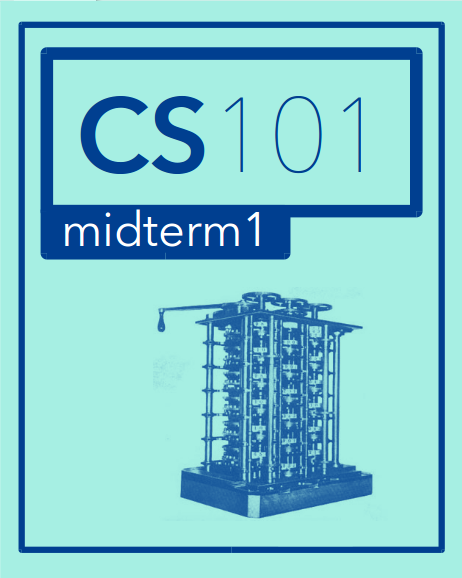
\includegraphics[width=2in]{../img/midterm1-header.png}
\end{center}

\bigskip
\noindent
\begin{itemize}
\item \textbf{Be sure to enter your \underline{NetID} and \underline{the code below} on your Scantron}.
\item Do not turn this page until instructed to do so.
\item There are 30 questions, worth 1 point each.
\item Each question has only \textbf{one} correct answer.
\item You must not communicate with other students during this test.
\item No books, notes, or electronic devices are permitted.
\item This is a 60-minute exam.
\item There are several different versions of this exam.
\end{itemize}

\bigskip\bigskip
\noindent
\textbf{\Large 1. Fill in your information:}

\bigskip
{\Large\bf
\begin{tabular}{ll}
Full Name: & \underbar{\hskip 8cm} \\[0.5em]
UIN (Student Number): & \underbar{\hskip 8cm} \\[0.5em]
NetID: & \underbar{\hskip 8cm}
\end{tabular}
}

\bigskip
\bigskip
\noindent
\textbf{\Large 2. Fill in the following answers on the Scantron form:}

%%%%%%%%%%%%%%%%%%%%%%%%%%%%%%%%%%%%%%%%%%%%%%%%%%%%%%%%%
%%%%%%%%%%%%%%%%%%%%%%%%%%%%%%%%%%%%%%%%%%%%%%%%%%%%%%%%%

\begin{enumerate}
\item[92.] B
\item[93.] C
\item[94.] B
\item[95.] C
\item[96.] A
\end{enumerate}

\newpage

% Zone 1


%%%%%%%%%%%%%%%%%%%%%%%%%%%%%%%%%%%%%%%%%%%%%%%%%%%%%%%%%



\newpage
\noindent
1. (1 point)
Consider the following program:
\begin{verbatim}
x=2
a=6
if (a%3)==2:
    x=x**3
elif(a%3)==1:
    x=x**2
else:
    x=x**1
\end{verbatim}
What is the \textbf{value} of \texttt{x} after this program is executed?


\begin{enumerate}
\item[(A)]
\begin{verbatim}16\end{verbatim}

\item[(B)]
\begin{verbatim}8\end{verbatim}

\item[(C)] $\bigstar$ 
\begin{verbatim}2\end{verbatim}

\item[(D)]
None of the other answers are correct.

\item[(E)]
\begin{verbatim}4\end{verbatim}

\end{enumerate}

\vspace*{2em}
\hrule
\vspace{2em}

\noindent {\bf Solution.} 
\vspace{2em}
\hrule height 2pt


\newpage
\noindent
2. (1 point)
Consider the following program:
\begin{verbatim}
s="TRIS %i"
t="ISEU"
x=len(s) % len(t[2:-1])
\end{verbatim}
What is the \textbf{type} of \texttt{x} after this program is executed?


\begin{enumerate}
\item[(A)]
\begin{verbatim}String\end{verbatim}

\item[(B)] $\bigstar$ 
\begin{verbatim}Integer\end{verbatim}

\item[(C)]
\begin{verbatim}Float\end{verbatim}

\item[(D)]
\begin{verbatim}None\end{verbatim}

\item[(E)]
\begin{verbatim}Boolean\end{verbatim}

\end{enumerate}

\vspace*{2em}
\hrule
\vspace{2em}

\noindent {\bf Solution.} 
\vspace{2em}
\hrule height 2pt


\newpage
\noindent
3. (1 point)
For this problem, you should compose a function which accomplishes a given task using the available code blocks arranged in the correct functional order.  \emph{We ignore indentation for this problem.}

\texttt{find\_max} should accept a \texttt{list} and return the value of the maximum item in the \texttt{list}.  (\texttt{None} is always the lowest value in any numeric comparison, so you may use it as an initializer.)

\begin{verbatim}
def find_max(my_list):
\end{verbatim}

\begin{enumerate}[1]
\item \texttt{max\_val = i}
\item \texttt{max\_val = None}
\item \texttt{for i in range(len(my\_list)):}
\item \texttt{if i > max\_val:}
\item \texttt{max\_val = my\_list[i]}
\item \texttt{return max\_val}
\item \texttt{for i in range(my\_list):}
\item \texttt{if my\_list[i] > max\_val:}
\item \texttt{print(max\_val)}
\end{enumerate}



\begin{enumerate}
\item[(A)]
3, 2, 8, 5, 9

\item[(B)]
2, 3, 8, 1, 6

\item[(C)]
2, 7, 4, 5, 6

\item[(D)]
2, 3, 4, 1, 6

\item[(E)] $\bigstar$ 
2, 3, 8, 5, 6

\end{enumerate}

\vspace*{2em}
\hrule
\vspace{2em}

\noindent {\bf Solution.} 
\vspace{2em}
\hrule height 2pt


\newpage
\noindent
4. (1 point)
Consider the following program:
\begin{verbatim}
x=[2,3,4,5,6,7,8,9]
x=x[2:-2]
i=1
while i <= 3:
    x[i]+=1
    i+=1
\end{verbatim}
What is the \textbf{value} of \texttt{x} after this program is executed?


\begin{enumerate}
\item[(A)]
\begin{verbatim}[3, 4, 6, 7, 8]\end{verbatim}

\item[(B)] $\bigstar$ 
\begin{verbatim}[4, 6, 7, 8]\end{verbatim}

\item[(C)]
\begin{verbatim}[4, 6, 7, 7]\end{verbatim}

\item[(D)]
\begin{verbatim}[2, 4, 6, 6]\end{verbatim}

\item[(E)]
\begin{verbatim}[4, 6, 7]\end{verbatim}

\end{enumerate}

\vspace*{2em}
\hrule
\vspace{2em}

\noindent {\bf Solution.} 
\vspace{2em}
\hrule height 2pt


\newpage
\noindent
5. (1 point)
Consider the following program.
\begin{verbatim}
def artificing(s):
    return s*2
    return s+"%i" % 2
    return s

s=artificing("MERLIN")
\end{verbatim}
After it is run, what is the final \textbf{value} of s?


\begin{enumerate}
\item[(A)]
\begin{verbatim}12\end{verbatim}

\item[(B)]
\begin{verbatim}"MERLIN2"\end{verbatim}

\item[(C)]
\begin{verbatim}"MERLIN"\end{verbatim}

\item[(D)]
\begin{verbatim}None\end{verbatim}

\item[(E)] $\bigstar$ 
\begin{verbatim}"MERLINMERLIN"\end{verbatim}

\end{enumerate}

\vspace*{2em}
\hrule
\vspace{2em}

\noindent {\bf Solution.} 
\vspace{2em}
\hrule height 2pt


\newpage
\noindent
6. (1 point)
Consider the following program:
\begin{verbatim}
i=3
x=2
while i < 7:
    x+=i
    i+=2
\end{verbatim}
What is the \textbf{value} of \texttt{x} after this program is executed?


\begin{enumerate}
\item[(A)] $\bigstar$ 
\begin{verbatim}10\end{verbatim}

\item[(B)]
\begin{verbatim}13\end{verbatim}

\item[(C)]
\begin{verbatim}11\end{verbatim}

\item[(D)]
\begin{verbatim}14\end{verbatim}

\item[(E)]
\begin{verbatim}12\end{verbatim}

\end{enumerate}

\vspace*{2em}
\hrule
\vspace{2em}

\noindent {\bf Solution.} 
\vspace{2em}
\hrule height 2pt


\newpage
\noindent
7. (1 point)
Consider the following incomplete Python program.
\begin{verbatim}
s="".join(["2","2","0","1"])
x=0
for i in range(len(s)-1):
    x+=int(???)
\end{verbatim}
What should replace the three question marks so the resulting value of \texttt{x} is 43?


\begin{enumerate}
\item[(A)]
\begin{verbatim}s[i:i+1]\end{verbatim}

\item[(B)]
\begin{verbatim}s[i:i-1]\end{verbatim}

\item[(C)] $\bigstar$ 
\begin{verbatim}s[i:i+2]\end{verbatim}

\item[(D)]
\begin{verbatim}s[i+1:i+2]\end{verbatim}

\end{enumerate}

\vspace*{2em}
\hrule
\vspace{2em}

\noindent {\bf Solution.} 
\vspace{2em}
\hrule height 2pt


\newpage
\noindent
8. (1 point)
Consider the following program:
\begin{verbatim}
s="ECTOR"
t="GAWAIN"
x=len(str(s.isupper()))-t.find("A")
\end{verbatim}
What is the \textbf{type} of \texttt{x} after this program is executed?


\begin{enumerate}
\item[(A)]
\begin{verbatim}Float\end{verbatim}

\item[(B)] $\bigstar$ 
\begin{verbatim}Integer\end{verbatim}

\item[(C)]
\begin{verbatim}Boolean\end{verbatim}

\item[(D)]
\begin{verbatim}None\end{verbatim}

\item[(E)]
\begin{verbatim}String\end{verbatim}

\end{enumerate}

\vspace*{2em}
\hrule
\vspace{2em}

\noindent {\bf Solution.} 
\vspace{2em}
\hrule height 2pt


\newpage
\noindent
9. (1 point)
Consider the following program:
\begin{verbatim}
def fix(s):
    a=list(s)
    a.sort()
    return ''.join(a)

x=["one","two","eleven","twelve"]
s1=fix(x[0]+x[-1])
s2=fix(x[1]+x[-2])

if s1<s2:
    x.sort()
elif s1==s2:
    x.reverse()
else:
    x.append("six")
\end{verbatim}
What is the \textbf{value} of \texttt{x} after this program is executed?


\begin{enumerate}
\item[(A)]
\begin{verbatim}['two', 'twelve', 'one', 'eleven', 'six']\end{verbatim}

\item[(B)]
\begin{verbatim}['one', 'two', 'eleven', 'twelve', 'six']\end{verbatim}

\item[(C)] $\bigstar$ 
\begin{verbatim}['twelve', 'eleven', 'two', 'one']\end{verbatim}

\item[(D)]
\begin{verbatim}['one', 'two', 'eleven', 'twelve']\end{verbatim}

\item[(E)]
\begin{verbatim}['eleven', 'one', 'twelve', 'two']\end{verbatim}

\end{enumerate}

\vspace*{2em}
\hrule
\vspace{2em}

\noindent {\bf Solution.} 
\vspace{2em}
\hrule height 2pt


\newpage
\noindent
10. (1 point)
Consider the following program.
\begin{verbatim}
kay = 2
wart = 3

def knight(kay,wart):
    wart += 2
    kay += 3
    return wart + kay

kay = knight(wart, kay) + knight(kay, wart)
\end{verbatim}
After it is run, what is the final \textbf{value} of \texttt{kay}?


\begin{enumerate}
\item[(A)]
\begin{verbatim}3\end{verbatim}

\item[(B)]
\begin{verbatim}5\end{verbatim}

\item[(C)] $\bigstar$ 
None of the other answers are correct.

\item[(D)]
\begin{verbatim}2\end{verbatim}

\end{enumerate}

\vspace*{2em}
\hrule
\vspace{2em}

\noindent {\bf Solution.} 
\vspace{2em}
\hrule height 2pt


\newpage
\noindent
11. (1 point)
Consider the following program:
\begin{verbatim}
pi="3.14159"
e="2.71828"
x=pi in pi*len(e)
\end{verbatim}
What is the \textbf{type} of \texttt{x} after this program is executed?


\begin{enumerate}
\item[(A)]
\begin{verbatim}String\end{verbatim}

\item[(B)] $\bigstar$ 
\begin{verbatim}Boolean\end{verbatim}

\item[(C)]
\begin{verbatim}Integer\end{verbatim}

\item[(D)]
\begin{verbatim}None\end{verbatim}

\item[(E)]
\begin{verbatim}Float\end{verbatim}

\end{enumerate}

\vspace*{2em}
\hrule
\vspace{2em}

\noindent {\bf Solution.} 
\vspace{2em}
\hrule height 2pt


\newpage
\noindent
12. (1 point)
Consider the following Python program.
\begin{verbatim}
e=[1,3,5,7,9,11]
d=[0,0,0]
for i in range(0,len(e)):
    d[i%3]+=e[i]
x=d[1]
\end{verbatim}
After it is run, what is the final \textbf{value} of \texttt{x}?


\begin{enumerate}
\item[(A)]
\begin{verbatim}16\end{verbatim}

\item[(B)] $\bigstar$ 
\begin{verbatim}12\end{verbatim}

\item[(C)]
\begin{verbatim}0\end{verbatim}

\item[(D)]
\begin{verbatim}8\end{verbatim}

\item[(E)]
\begin{verbatim}3\end{verbatim}

\end{enumerate}

\vspace*{2em}
\hrule
\vspace{2em}

\noindent {\bf Solution.} 
\vspace{2em}
\hrule height 2pt


\newpage
\noindent
13. (1 point)
Consider the following program:
\begin{verbatim}
a=3
b=4
if a==3:
    a=b
elif a==4:
    a=5
else:
    b=a
\end{verbatim}
What is the \textbf{value} of a after this program is executed?


\begin{enumerate}
\item[(A)] $\bigstar$ 
\begin{verbatim}4\end{verbatim}

\item[(B)]
\begin{verbatim}5\end{verbatim}

\item[(C)]
None of the other answers are correct.

\item[(D)]
\begin{verbatim}7\end{verbatim}

\item[(E)]
\begin{verbatim}3\end{verbatim}

\end{enumerate}

\vspace*{2em}
\hrule
\vspace{2em}

\noindent {\bf Solution.} 
\vspace{2em}
\hrule height 2pt


\newpage
\noindent
14. (1 point)
Consider the following program:
\begin{verbatim}
s="Calvin"
i=0
x=-1
while i<len(s):
    if s[i]=='b':
        x=i
    i+=1
\end{verbatim}
What is the \textbf{value} of \texttt{x} after this program is executed?


\begin{enumerate}
\item[(A)]
\begin{verbatim}6\end{verbatim}

\item[(B)]
\begin{verbatim}3\end{verbatim}

\item[(C)]
\begin{verbatim}5\end{verbatim}

\item[(D)]
\begin{verbatim}0\end{verbatim}

\item[(E)] $\bigstar$ 
\begin{verbatim}-1\end{verbatim}

\end{enumerate}

\vspace*{2em}
\hrule
\vspace{2em}

\noindent {\bf Solution.} 
\vspace{2em}
\hrule height 2pt


\newpage
\noindent
15. (1 point)
Consider the following program:
\begin{verbatim}
x="KING ARTHUR-MORGANA LEFAY-SIR BEDIVERE".split("-")
y=x[:]
y.reverse()
\end{verbatim}
What is the \textbf{value} of \texttt{x} after this program is executed?


\begin{enumerate}
\item[(A)]
\begin{verbatim}['BEDIVERE', 'LEFAY-SIR', 'ARTHUR-MORGANA', 'KING']\end{verbatim}

\item[(B)]
\begin{verbatim}['KING', 'ARTHUR-MORGANA', 'LEFAY-SIR', 'BEDIVERE']\end{verbatim}

\item[(C)]
\begin{verbatim}['SIR BEDIVERE', 'MORGANA LEFAY', 'KING ARTHUR']\end{verbatim}

\item[(D)] $\bigstar$ 
\begin{verbatim}['KING ARTHUR', 'MORGANA LEFAY', 'SIR BEDIVERE']\end{verbatim}

\item[(E)]
\begin{verbatim}None\end{verbatim}

\end{enumerate}

\vspace*{2em}
\hrule
\vspace{2em}

\noindent {\bf Solution.} 
\vspace{2em}
\hrule height 2pt


\newpage
\noindent
16. (1 point)
Consider the following program:
\begin{verbatim}
s="-B-O-R-S-"
x=s.split("-")[2:-2]
\end{verbatim}
What is the \textbf{value} of \texttt{x} after this program is executed?


\begin{enumerate}
\item[(A)]
\begin{verbatim}None\end{verbatim}

\item[(B)]
\begin{verbatim}'ORS'\end{verbatim}

\item[(C)]
\begin{verbatim}False\end{verbatim}

\item[(D)]
\begin{verbatim}''\end{verbatim}

\item[(E)] $\bigstar$ 
\begin{verbatim}['O', 'R']\end{verbatim}

\end{enumerate}

\vspace*{2em}
\hrule
\vspace{2em}

\noindent {\bf Solution.} 
\vspace{2em}
\hrule height 2pt


\newpage
\noindent
17. (1 point)
Consider the following program.
\begin{verbatim}
s="ABCBA"
x=0
y=len(s)-1
while s[x]==s[y] and x<y:
    x+=1
    y-=1
\end{verbatim}
After it is run, what is the final \textbf{value} of \texttt{x}?


\begin{enumerate}
\item[(A)] $\bigstar$ 
\begin{verbatim}2\end{verbatim}

\item[(B)]
\begin{verbatim}0\end{verbatim}

\item[(C)]
\begin{verbatim}3\end{verbatim}

\item[(D)]
\begin{verbatim}1\end{verbatim}

\item[(E)]
\begin{verbatim}4\end{verbatim}

\end{enumerate}

\vspace*{2em}
\hrule
\vspace{2em}

\noindent {\bf Solution.} 
\vspace{2em}
\hrule height 2pt


\newpage
\noindent
18. (1 point)
Consider the following program.
\begin{verbatim}
x=[]
for j in range(0,5):
    if (j%4)==0:
        x.append("-")
    if (j%5)==0:
        x.append("*")
\end{verbatim}
After it is run, what is the final \textbf{value} of \texttt{x}?


\begin{enumerate}
\item[(A)]
\begin{verbatim}["-","*","*"]\end{verbatim}

\item[(B)]
None of the other answers are correct.

\item[(C)] $\bigstar$ 
\begin{verbatim}["-","*","-"]\end{verbatim}

\item[(D)]
\begin{verbatim}["-","*"]\end{verbatim}

\item[(E)]
\begin{verbatim}["-","-","*"]\end{verbatim}

\end{enumerate}

\vspace*{2em}
\hrule
\vspace{2em}

\noindent {\bf Solution.} 
\vspace{2em}
\hrule height 2pt


\newpage
\noindent
19. (1 point)
Consider the following incomplete function.
\begin{verbatim}
def isdivisible(m,n):
    if ???:
        return False
    else:
        return True
\end{verbatim}
The function is intended to return True if the input parameter m is evenly divisible by the parameter n and False otherwise. For example, \verb|isdivisible(4,2)| should return \verb|True|, but \verb|isdivisible(5,3)| should return \verb|False|. What should replace the three question marks to complete the function?


\begin{enumerate}
\item[(A)]
\begin{verbatim}(n // m) == 0 \end{verbatim}

\item[(B)]
\begin{verbatim}(n % m) == 0 \end{verbatim}

\item[(C)] $\bigstar$ 
\begin{verbatim}(m % n) != 0 \end{verbatim}

\item[(D)]
\begin{verbatim}(m // n) != 0 \end{verbatim}

\end{enumerate}

\vspace*{2em}
\hrule
\vspace{2em}

\noindent {\bf Solution.} 
\vspace{2em}
\hrule height 2pt


\newpage
\noindent
20. (1 point)
Consider the following incomplete program.
\begin{verbatim}
sum=0
???:
    sum=sum+i

\end{verbatim}
The program is intended to sum all of the integers between 1 and 100 (inclusive). What should replace the three question marks to complete the program?


\begin{enumerate}
\item[(A)]
\begin{verbatim}for i in range(0,100)\end{verbatim}

\item[(B)]
\begin{verbatim}while i in range(100)\end{verbatim}

\item[(C)]
\begin{verbatim}while i<=100 \end{verbatim}

\item[(D)] $\bigstar$ 
\begin{verbatim}for i in range(1,101) \end{verbatim}

\end{enumerate}

\vspace*{2em}
\hrule
\vspace{2em}

\noindent {\bf Solution.} 
\vspace{2em}
\hrule height 2pt


\newpage
\noindent
21. (1 point)
Evaluate the following expression:
\begin{verbatim}
len("ABCD"[0:3])
\end{verbatim}
What value is produced?


\begin{enumerate}
\item[(A)]
2

\item[(B)]
1

\item[(C)] $\bigstar$ 
3

\item[(D)]
4

\end{enumerate}

\vspace*{2em}
\hrule
\vspace{2em}

\noindent {\bf Solution.} 
\vspace{2em}
\hrule height 2pt


\newpage
\noindent
22. (1 point)
How can the following mathematical equation be implemented as a Python expression? Assume \verb|a|, \verb|b|, and \verb|sin| have already been defined.
$$a \sin(a^b - b)$$


\begin{enumerate}
\item[(A)]
\begin{verbatim}a*sin(b^a - b)\end{verbatim}

\item[(B)]
\begin{verbatim}a sin(a**b - b)\end{verbatim}

\item[(C)] $\bigstar$ 
\begin{verbatim}a*sin(a**b - b)\end{verbatim}

\item[(D)]
\begin{verbatim}a*sin(a^b - b)\end{verbatim}

\item[(E)]
None of the other answers are correct.

\end{enumerate}

\vspace*{2em}
\hrule
\vspace{2em}

\noindent {\bf Solution.} 
\vspace{2em}
\hrule height 2pt


\newpage
\noindent
23. (1 point)
Consider the following program:
\begin{verbatim}
x=0
for i in range(4,10):
    if i%3==0:
        x+=3
    elif i%2==0:
        x+=2
    else:
        x+=1
\end{verbatim}
What is the \textbf{value} of \texttt{x} after this program is executed?


\begin{enumerate}
\item[(A)]
\begin{verbatim}10\end{verbatim}

\item[(B)]
\begin{verbatim}14\end{verbatim}

\item[(C)] $\bigstar$ 
\begin{verbatim}12\end{verbatim}

\item[(D)]
\begin{verbatim}11\end{verbatim}

\item[(E)]
\begin{verbatim}13\end{verbatim}

\end{enumerate}

\vspace*{2em}
\hrule
\vspace{2em}

\noindent {\bf Solution.} 
\vspace{2em}
\hrule height 2pt


\newpage
\noindent
24. (1 point)
Evaluate the following expression:
\begin{verbatim}
[1,2]*len("3")
\end{verbatim}
What value is produced?


\begin{enumerate}
\item[(A)]
\begin{verbatim}[1,2,1,2,1,2]\end{verbatim}

\item[(B)]
\begin{verbatim}[1,2,3]\end{verbatim}

\item[(C)] $\bigstar$ 
\begin{verbatim}[1,2]\end{verbatim}

\item[(D)]
\begin{verbatim}[1,2,1]\end{verbatim}

\end{enumerate}

\vspace*{2em}
\hrule
\vspace{2em}

\noindent {\bf Solution.} 
\vspace{2em}
\hrule height 2pt


\newpage
\noindent
25. (1 point)
What is the result of the following expression?
\begin{verbatim}
[ 1, 2, 3 ] * 3.0
\end{verbatim}


\begin{enumerate}
\item[(A)]
\begin{verbatim}[3.0, 6.0, 9.0]\end{verbatim}

\item[(B)]
\begin{verbatim}[1.0, 2.0, 3.0, 1.0, 2.0, 3.0, 1.0, 2.0, 3.0]\end{verbatim}

\item[(C)]
\begin{verbatim}None of the above.\end{verbatim}

\item[(D)]
\begin{verbatim}[3, 6, 9]\end{verbatim}

\item[(E)] $\bigstar$ 
\begin{verbatim}[1, 2, 3, 1, 2, 3, 1, 2, 3]\end{verbatim}

\end{enumerate}

\vspace*{2em}
\hrule
\vspace{2em}

\noindent {\bf Solution.} 
\vspace{2em}
\hrule height 2pt


\newpage
\noindent
26. (1 point)
Consider the following program:
\begin{verbatim}
a=["S","T","U","P","E","F","Y"]
a=a[0:4]
a.sort()
x=""
for e in a:
    x=e+x
\end{verbatim}
What is the \textbf{value} of \texttt{x} after this program is executed?


\begin{enumerate}
\item[(A)]
None of the other answers are correct.

\item[(B)] $\bigstar$ 
\begin{verbatim}"UTSP"\end{verbatim}

\item[(C)]
\begin{verbatim}"STUP"\end{verbatim}

\item[(D)]
\begin{verbatim}"PSTU"\end{verbatim}

\item[(E)]
\begin{verbatim}"PUST"\end{verbatim}

\end{enumerate}

\vspace*{2em}
\hrule
\vspace{2em}

\noindent {\bf Solution.} 
\vspace{2em}
\hrule height 2pt


\newpage
\noindent
27. (1 point)
Consider the following program:
\begin{verbatim}
a=["merlin","sir agravaine","king pellinore"]
b=[ ]
for i in range(0,4):
    b.append(a[0-i].title())
\end{verbatim}
What is the \textbf{value} of b after this program is executed?


\begin{enumerate}
\item[(A)]
\begin{verbatim}[ ]\end{verbatim}

\item[(B)]
\begin{verbatim}['Merlin', 'King Pellinore', 'Sir Agravaine']\end{verbatim}

\item[(C)]
\begin{verbatim}['King Pellinore', 'Sir Agravaine', 'Merlin']\end{verbatim}

\item[(D)] $\bigstar$ 
\begin{verbatim}['Merlin', 'King Pellinore', 'Sir Agravaine', 'Merlin']\end{verbatim}

\item[(E)]
\begin{verbatim}['Merlin', 'Sir Agravaine', 'King Pellinore', 'Merlin']\end{verbatim}

\end{enumerate}

\vspace*{2em}
\hrule
\vspace{2em}

\noindent {\bf Solution.} 
\vspace{2em}
\hrule height 2pt


\newpage
\noindent
28. (1 point)
Consider the following program.
\begin{verbatim}
x=0
i=1
while(i*i)<=9:
    x=x+(i*i)
    i=i+1
\end{verbatim}
After it is run, what is the final \textbf{value} of \texttt{x}?


\begin{enumerate}
\item[(A)]
\begin{verbatim}3\end{verbatim}

\item[(B)] $\bigstar$ 
\begin{verbatim}14\end{verbatim}

\item[(C)]
\begin{verbatim}30\end{verbatim}

\item[(D)]
\begin{verbatim}5\end{verbatim}

\item[(E)]
\begin{verbatim}4\end{verbatim}

\end{enumerate}

\vspace*{2em}
\hrule
\vspace{2em}

\noindent {\bf Solution.} 
\vspace{2em}
\hrule height 2pt


\newpage
\noindent
29. (1 point)
Consider the following program:
\begin{verbatim}
x=[1,2,3]
def f(a):
    s=""
    a.reverse()
    for i in a:
        s+=str(i)
    return s

x.append(f(x))
\end{verbatim}
What is the \textbf{value} of \texttt{x} after this program is executed?


\begin{enumerate}
\item[(A)]
\begin{verbatim}[1, 2, 3]\end{verbatim}

\item[(B)]
\begin{verbatim}[1, 2, 3, '321']\end{verbatim}

\item[(C)]
\begin{verbatim}[3, 2, 1]\end{verbatim}

\item[(D)]
\begin{verbatim}[1, 2, 3, 6]\end{verbatim}

\item[(E)] $\bigstar$ 
\begin{verbatim}[3, 2, 1, '321']\end{verbatim}

\end{enumerate}

\vspace*{2em}
\hrule
\vspace{2em}

\noindent {\bf Solution.} 
\vspace{2em}
\hrule height 2pt


\newpage
\noindent
30. (1 point)
\begin{verbatim}
x=str(3)+"str(3)"
\end{verbatim}
What is the \textbf{value} of \texttt{x} after this program is executed?


\begin{enumerate}
\item[(A)]
\begin{verbatim}33\end{verbatim}

\item[(B)] $\bigstar$ 
\begin{verbatim}"3str(3)"\end{verbatim}

\item[(C)]
\begin{verbatim}"33"\end{verbatim}

\item[(D)]
\begin{verbatim}"333"\end{verbatim}

\item[(E)]
None of the other answers are correct.

\end{enumerate}

\vspace*{2em}
\hrule
\vspace{2em}

\noindent {\bf Solution.} 
\vspace{2em}
\hrule height 2pt

%%%%%%%%%%%%%%%%%%%%%%%%%%%%%%%%%%%%%%%%%%%%%%%%%%%%%%%%%%%%%%%%%%%%%%
%%%%%%%%%%%%%%%%%%%%%%%%%%%%%%%%%%%%%%%%%%%%%%%%%%%%%%%%%%%%%%%%%%%%%%
%%%%%%%%%%%%%%%%%%%%%%%%%%%%%%%%%%%%%%%%%%%%%%%%%%%%%%%%%%%%%%%%%%%%%%
%%%%%%%%%%%%%%%%%%%%%%%%%%%%%%%%%%%%%%%%%%%%%%%%%%%%%%%%%%%%%%%%%%%%%%
% Exam number 38

\message{Exam 38/50}
\cleardoublepage
\setcounter{page}{1}


\begin{center}
%\textbf{\Large CS 101 Midterm \#1}
%
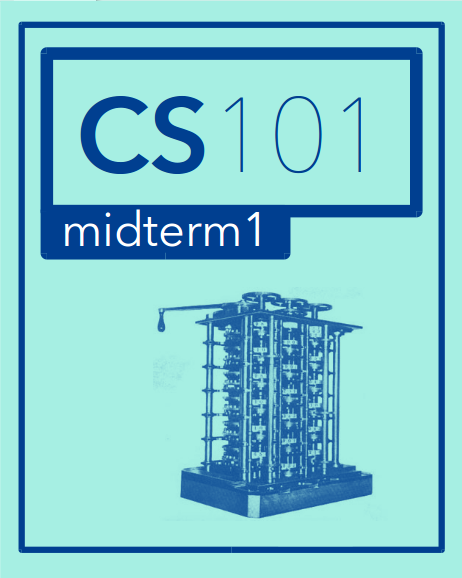
\includegraphics[width=2in]{../img/midterm1-header.png}
\end{center}

\bigskip
\noindent
\begin{itemize}
\item \textbf{Be sure to enter your \underline{NetID} and \underline{the code below} on your Scantron}.
\item Do not turn this page until instructed to do so.
\item There are 30 questions, worth 1 point each.
\item Each question has only \textbf{one} correct answer.
\item You must not communicate with other students during this test.
\item No books, notes, or electronic devices are permitted.
\item This is a 60-minute exam.
\item There are several different versions of this exam.
\end{itemize}

\bigskip\bigskip
\noindent
\textbf{\Large 1. Fill in your information:}

\bigskip
{\Large\bf
\begin{tabular}{ll}
Full Name: & \underbar{\hskip 8cm} \\[0.5em]
UIN (Student Number): & \underbar{\hskip 8cm} \\[0.5em]
NetID: & \underbar{\hskip 8cm}
\end{tabular}
}

\bigskip
\bigskip
\noindent
\textbf{\Large 2. Fill in the following answers on the Scantron form:}

%%%%%%%%%%%%%%%%%%%%%%%%%%%%%%%%%%%%%%%%%%%%%%%%%%%%%%%%%
%%%%%%%%%%%%%%%%%%%%%%%%%%%%%%%%%%%%%%%%%%%%%%%%%%%%%%%%%

\begin{enumerate}
\item[92.] C
\item[93.] C
\item[94.] B
\item[95.] D
\item[96.] B
\end{enumerate}

\newpage

% Zone 1


%%%%%%%%%%%%%%%%%%%%%%%%%%%%%%%%%%%%%%%%%%%%%%%%%%%%%%%%%



\newpage
\noindent
1. (1 point)
Consider the following program.
\begin{verbatim}
s="ABCBA"
x=0
y=len(s)-1
while s[x]==s[y] and x<y:
    x+=1
    y-=1
\end{verbatim}
After it is run, what is the final \textbf{value} of \texttt{x}?


\begin{enumerate}
\item[(A)]
\begin{verbatim}4\end{verbatim}

\item[(B)]
\begin{verbatim}0\end{verbatim}

\item[(C)] $\bigstar$ 
\begin{verbatim}2\end{verbatim}

\item[(D)]
\begin{verbatim}1\end{verbatim}

\item[(E)]
\begin{verbatim}3\end{verbatim}

\end{enumerate}

\vspace*{2em}
\hrule
\vspace{2em}

\noindent {\bf Solution.} 
\vspace{2em}
\hrule height 2pt


\newpage
\noindent
2. (1 point)
Consider the following program:
\begin{verbatim}
x=0
for i in range(2,8):
    if i%3==0:
        x+=3
    elif i%2==0:
        x+=2
    else:
        x+=1
\end{verbatim}
What is the \textbf{value} of \texttt{x} after this program is executed?


\begin{enumerate}
\item[(A)]
\begin{verbatim}10\end{verbatim}

\item[(B)]
\begin{verbatim}14\end{verbatim}

\item[(C)] $\bigstar$ 
\begin{verbatim}12\end{verbatim}

\item[(D)]
\begin{verbatim}11\end{verbatim}

\item[(E)]
\begin{verbatim}13\end{verbatim}

\end{enumerate}

\vspace*{2em}
\hrule
\vspace{2em}

\noindent {\bf Solution.} 
\vspace{2em}
\hrule height 2pt


\newpage
\noindent
3. (1 point)
For this problem, you should compose a function which accomplishes a given task using the available code blocks arranged in the correct functional order.  \emph{We ignore indentation for this problem.}

\texttt{find\_max} should accept a \texttt{list} and return the value of the maximum item in the \texttt{list}.  (\texttt{None} is always the lowest value in any numeric comparison, so you may use it as an initializer.)

\begin{verbatim}
def find_max(my_list):
\end{verbatim}

\begin{enumerate}[1]
\item \texttt{max\_val = i}
\item \texttt{max\_val = None}
\item \texttt{for i in range(len(my\_list)):}
\item \texttt{if i > max\_val:}
\item \texttt{max\_val = my\_list[i]}
\item \texttt{return max\_val}
\item \texttt{for i in range(my\_list):}
\item \texttt{if my\_list[i] > max\_val:}
\item \texttt{print(max\_val)}
\end{enumerate}



\begin{enumerate}
\item[(A)]
2, 3, 4, 1, 6

\item[(B)]
2, 7, 4, 5, 6

\item[(C)]
3, 2, 8, 5, 9

\item[(D)]
2, 3, 8, 1, 6

\item[(E)] $\bigstar$ 
2, 3, 8, 5, 6

\end{enumerate}

\vspace*{2em}
\hrule
\vspace{2em}

\noindent {\bf Solution.} 
\vspace{2em}
\hrule height 2pt


\newpage
\noindent
4. (1 point)
Consider the following incomplete Python program.
\begin{verbatim}
s="".join(["0","1","2","1"])
x=0
for i in range(len(s)-1):
    x+=int(???)
\end{verbatim}
What should replace the three question marks so the resulting value of \texttt{x} is 34?


\begin{enumerate}
\item[(A)] $\bigstar$ 
\begin{verbatim}s[i:i+2]\end{verbatim}

\item[(B)]
\begin{verbatim}s[i+1:i+2]\end{verbatim}

\item[(C)]
\begin{verbatim}s[i:i+1]\end{verbatim}

\item[(D)]
\begin{verbatim}s[i:i-1]\end{verbatim}

\end{enumerate}

\vspace*{2em}
\hrule
\vspace{2em}

\noindent {\bf Solution.} 
\vspace{2em}
\hrule height 2pt


\newpage
\noindent
5. (1 point)
Consider the following program:
\begin{verbatim}
x=[1,2,3]
def f(a):
    s=""
    a.reverse()
    for i in a:
        s+=str(i)
    return s

x.append(f(x))
\end{verbatim}
What is the \textbf{value} of \texttt{x} after this program is executed?


\begin{enumerate}
\item[(A)]
\begin{verbatim}[1, 2, 3, '321']\end{verbatim}

\item[(B)]
\begin{verbatim}[3, 2, 1]\end{verbatim}

\item[(C)] $\bigstar$ 
\begin{verbatim}[3, 2, 1, '321']\end{verbatim}

\item[(D)]
\begin{verbatim}[1, 2, 3, 6]\end{verbatim}

\item[(E)]
\begin{verbatim}[1, 2, 3]\end{verbatim}

\end{enumerate}

\vspace*{2em}
\hrule
\vspace{2em}

\noindent {\bf Solution.} 
\vspace{2em}
\hrule height 2pt


\newpage
\noindent
6. (1 point)
Consider the following program:
\begin{verbatim}
a=3
b=4
if a==3:
    b=a
elif a==4:
    a=5
else:
    a=b
\end{verbatim}
What is the \textbf{value} of a after this program is executed?


\begin{enumerate}
\item[(A)]
\begin{verbatim}5\end{verbatim}

\item[(B)]
\begin{verbatim}4\end{verbatim}

\item[(C)]
None of the other answers are correct.

\item[(D)] $\bigstar$ 
\begin{verbatim}3\end{verbatim}

\item[(E)]
\begin{verbatim}7\end{verbatim}

\end{enumerate}

\vspace*{2em}
\hrule
\vspace{2em}

\noindent {\bf Solution.} 
\vspace{2em}
\hrule height 2pt


\newpage
\noindent
7. (1 point)
How can the following mathematical equation be implemented as a Python expression? Assume \verb|a|, \verb|b|, and \verb|sin| have already been defined.
$$a \sin(a^b - b)$$


\begin{enumerate}
\item[(A)]
\begin{verbatim}a*sin(a^b - b)\end{verbatim}

\item[(B)]
\begin{verbatim}a*sin(b^a - b)\end{verbatim}

\item[(C)]
\begin{verbatim}a sin(a**b - b)\end{verbatim}

\item[(D)]
None of the other answers are correct.

\item[(E)] $\bigstar$ 
\begin{verbatim}a*sin(a**b - b)\end{verbatim}

\end{enumerate}

\vspace*{2em}
\hrule
\vspace{2em}

\noindent {\bf Solution.} 
\vspace{2em}
\hrule height 2pt


\newpage
\noindent
8. (1 point)
Consider the following program.
\begin{verbatim}
x=0
i=1
while(i*i)<=9:
    x=x+(i*i)
    i=i+1
\end{verbatim}
After it is run, what is the final \textbf{value} of \texttt{x}?


\begin{enumerate}
\item[(A)]
\begin{verbatim}3\end{verbatim}

\item[(B)]
\begin{verbatim}30\end{verbatim}

\item[(C)]
\begin{verbatim}4\end{verbatim}

\item[(D)] $\bigstar$ 
\begin{verbatim}14\end{verbatim}

\item[(E)]
\begin{verbatim}5\end{verbatim}

\end{enumerate}

\vspace*{2em}
\hrule
\vspace{2em}

\noindent {\bf Solution.} 
\vspace{2em}
\hrule height 2pt


\newpage
\noindent
9. (1 point)
Consider the following program.
\begin{verbatim}
x=[]
for j in range(0,5):
    if (j%2)==0:
        x.append("-")
    if (j%5)==0:
        x.append("*")
\end{verbatim}
After it is run, what is the final \textbf{value} of \texttt{x}?


\begin{enumerate}
\item[(A)]
\begin{verbatim}["-","-","*"]\end{verbatim}

\item[(B)]
\begin{verbatim}["-","*","-"]\end{verbatim}

\item[(C)] $\bigstar$ 
\begin{verbatim}["-","*","-","-"]\end{verbatim}

\item[(D)]
\begin{verbatim}["*","-","*","*"]\end{verbatim}

\item[(E)]
None of the other answers are correct.

\end{enumerate}

\vspace*{2em}
\hrule
\vspace{2em}

\noindent {\bf Solution.} 
\vspace{2em}
\hrule height 2pt


\newpage
\noindent
10. (1 point)
Consider the following program:
\begin{verbatim}
s="-B-O-R-S-"
x=s.split("-")[2:-2]
\end{verbatim}
What is the \textbf{value} of \texttt{x} after this program is executed?


\begin{enumerate}
\item[(A)]
\begin{verbatim}None\end{verbatim}

\item[(B)]
\begin{verbatim}'ORS'\end{verbatim}

\item[(C)]
\begin{verbatim}''\end{verbatim}

\item[(D)] $\bigstar$ 
\begin{verbatim}['O', 'R']\end{verbatim}

\item[(E)]
\begin{verbatim}False\end{verbatim}

\end{enumerate}

\vspace*{2em}
\hrule
\vspace{2em}

\noindent {\bf Solution.} 
\vspace{2em}
\hrule height 2pt


\newpage
\noindent
11. (1 point)
Consider the following incomplete function.
\begin{verbatim}
def ismultiple(m,n):
    if ???:
        return False
    else:
        return True
\end{verbatim}
The function is intended to return True if the input parameter m is a multiple of parameter n and False otherwise. For example, \verb|ismultiple(4,2)| should return \verb|True|, but \verb|ismultiple(5,3)| should return \verb|False|. What should replace the three question marks to complete the function?


\begin{enumerate}
\item[(A)]
\begin{verbatim}(n % m) == 0 \end{verbatim}

\item[(B)]
\begin{verbatim}(n // m) == 0 \end{verbatim}

\item[(C)] $\bigstar$ 
\begin{verbatim}(m % n) != 0 \end{verbatim}

\item[(D)]
\begin{verbatim}(m // n) != 0 \end{verbatim}

\end{enumerate}

\vspace*{2em}
\hrule
\vspace{2em}

\noindent {\bf Solution.} 
\vspace{2em}
\hrule height 2pt


\newpage
\noindent
12. (1 point)
Consider the following program:
\begin{verbatim}
s="Hobbes"
i=0
x=-1
while i<len(s):
    if s[i]=='b':
        x=i
    i+=1
\end{verbatim}
What is the \textbf{value} of \texttt{x} after this program is executed?


\begin{enumerate}
\item[(A)]
\begin{verbatim}5\end{verbatim}

\item[(B)] $\bigstar$ 
\begin{verbatim}3\end{verbatim}

\item[(C)]
\begin{verbatim}2\end{verbatim}

\item[(D)]
\begin{verbatim}4\end{verbatim}

\item[(E)]
\begin{verbatim}-1\end{verbatim}

\end{enumerate}

\vspace*{2em}
\hrule
\vspace{2em}

\noindent {\bf Solution.} 
\vspace{2em}
\hrule height 2pt


\newpage
\noindent
13. (1 point)
Consider the following program:
\begin{verbatim}
a=["S","T","U","P","E","F","Y"]
a=a[0:4]
a.sort()
x=""
for e in a:
    x=e+x
\end{verbatim}
What is the \textbf{value} of \texttt{x} after this program is executed?


\begin{enumerate}
\item[(A)] $\bigstar$ 
\begin{verbatim}"UTSP"\end{verbatim}

\item[(B)]
\begin{verbatim}"PSTU"\end{verbatim}

\item[(C)]
None of the other answers are correct.

\item[(D)]
\begin{verbatim}"PUST"\end{verbatim}

\item[(E)]
\begin{verbatim}"STUP"\end{verbatim}

\end{enumerate}

\vspace*{2em}
\hrule
\vspace{2em}

\noindent {\bf Solution.} 
\vspace{2em}
\hrule height 2pt


\newpage
\noindent
14. (1 point)
Evaluate the following expression:
\begin{verbatim}
[1,2]*len("3")
\end{verbatim}
What value is produced?


\begin{enumerate}
\item[(A)]
\begin{verbatim}[1,2,1,2,1,2]\end{verbatim}

\item[(B)] $\bigstar$ 
\begin{verbatim}[1,2]\end{verbatim}

\item[(C)]
\begin{verbatim}[1,2,3]\end{verbatim}

\item[(D)]
\begin{verbatim}[1,2,1]\end{verbatim}

\end{enumerate}

\vspace*{2em}
\hrule
\vspace{2em}

\noindent {\bf Solution.} 
\vspace{2em}
\hrule height 2pt


\newpage
\noindent
15. (1 point)
Consider the following program:
\begin{verbatim}
x=[1,2,3,4,5,6,7,8,9]
x=x[2:-2]
i=1
while i < 3:
    x[i]+=1
    i+=1
\end{verbatim}
What is the \textbf{value} of \texttt{x} after this program is executed?


\begin{enumerate}
\item[(A)]
\begin{verbatim}[3, 5, 6, 6, 7, 8]\end{verbatim}

\item[(B)]
\begin{verbatim}[3, 5, 6, 6]\end{verbatim}

\item[(C)]
\begin{verbatim}[2, 4, 5, 6, 6, 7]\end{verbatim}

\item[(D)]
\begin{verbatim}[2, 4, 5, 5, 6, 7]\end{verbatim}

\item[(E)] $\bigstar$ 
\begin{verbatim}[3, 5, 6, 6, 7]\end{verbatim}

\end{enumerate}

\vspace*{2em}
\hrule
\vspace{2em}

\noindent {\bf Solution.} 
\vspace{2em}
\hrule height 2pt


\newpage
\noindent
16. (1 point)
Consider the following program.
\begin{verbatim}
kay = 2
wart = 3

def knight(kay,wart):
    wart += 2
    kay += 3
    return wart + kay

kay = knight(wart, kay) + knight(kay, wart)
\end{verbatim}
After it is run, what is the final \textbf{value} of \texttt{kay}?


\begin{enumerate}
\item[(A)]
\begin{verbatim}5\end{verbatim}

\item[(B)]
\begin{verbatim}2\end{verbatim}

\item[(C)]
\begin{verbatim}3\end{verbatim}

\item[(D)] $\bigstar$ 
None of the other answers are correct.

\end{enumerate}

\vspace*{2em}
\hrule
\vspace{2em}

\noindent {\bf Solution.} 
\vspace{2em}
\hrule height 2pt


\newpage
\noindent
17. (1 point)
Consider the following program:
\begin{verbatim}
x=3
a=7
if (a%3)==2:
    x=x**2
elif(a%3)==1:
    x=x**1
else:
    x=x**0
\end{verbatim}
What is the \textbf{value} of \texttt{x} after this program is executed?


\begin{enumerate}
\item[(A)]
\begin{verbatim}7\end{verbatim}

\item[(B)]
None of the other answers are correct.

\item[(C)]
\begin{verbatim}9\end{verbatim}

\item[(D)] $\bigstar$ 
\begin{verbatim}3\end{verbatim}

\item[(E)]
\begin{verbatim}1\end{verbatim}

\end{enumerate}

\vspace*{2em}
\hrule
\vspace{2em}

\noindent {\bf Solution.} 
\vspace{2em}
\hrule height 2pt


\newpage
\noindent
18. (1 point)
Consider the following program:
\begin{verbatim}
s="TRIS %i"
t="ISEU"
x=len(s) % len(t[2:-1])
\end{verbatim}
What is the \textbf{type} of \texttt{x} after this program is executed?


\begin{enumerate}
\item[(A)]
\begin{verbatim}String\end{verbatim}

\item[(B)]
\begin{verbatim}None\end{verbatim}

\item[(C)]
\begin{verbatim}Boolean\end{verbatim}

\item[(D)]
\begin{verbatim}Float\end{verbatim}

\item[(E)] $\bigstar$ 
\begin{verbatim}Integer\end{verbatim}

\end{enumerate}

\vspace*{2em}
\hrule
\vspace{2em}

\noindent {\bf Solution.} 
\vspace{2em}
\hrule height 2pt


\newpage
\noindent
19. (1 point)
What is the result of the following expression?
\begin{verbatim}
[ 1, 2, 3 ] * 3
\end{verbatim}


\begin{enumerate}
\item[(A)]
\begin{verbatim}(3, 6, 9)\end{verbatim}

\item[(B)]
\begin{verbatim}[1.0, 2.0, 3.0, 1.0, 2.0, 3.0, 1.0, 2.0, 3.0]\end{verbatim}

\item[(C)]
\begin{verbatim}[3, 6, 9]\end{verbatim}

\item[(D)]
\begin{verbatim}[3.0, 6.0, 9.0]\end{verbatim}

\item[(E)] $\bigstar$ 
\begin{verbatim}[1, 2, 3, 1, 2, 3, 1, 2, 3]\end{verbatim}

\end{enumerate}

\vspace*{2em}
\hrule
\vspace{2em}

\noindent {\bf Solution.} 
\vspace{2em}
\hrule height 2pt


\newpage
\noindent
20. (1 point)
Consider the following program:
\begin{verbatim}
i=3
x=2
while i < 7:
    x+=i
    i+=2
\end{verbatim}
What is the \textbf{value} of \texttt{x} after this program is executed?


\begin{enumerate}
\item[(A)]
\begin{verbatim}14\end{verbatim}

\item[(B)]
\begin{verbatim}11\end{verbatim}

\item[(C)]
\begin{verbatim}13\end{verbatim}

\item[(D)]
\begin{verbatim}12\end{verbatim}

\item[(E)] $\bigstar$ 
\begin{verbatim}10\end{verbatim}

\end{enumerate}

\vspace*{2em}
\hrule
\vspace{2em}

\noindent {\bf Solution.} 
\vspace{2em}
\hrule height 2pt


\newpage
\noindent
21. (1 point)
Consider the following incomplete program.
\begin{verbatim}
sum=0
???:
    sum=sum+i

\end{verbatim}
The program is intended to sum all of the integers between 1 and 100 (inclusive). What should replace the three question marks to complete the program?


\begin{enumerate}
\item[(A)]
\begin{verbatim}while i<=100 \end{verbatim}

\item[(B)]
\begin{verbatim}for i in range(0,100)\end{verbatim}

\item[(C)] $\bigstar$ 
\begin{verbatim}for i in range(1,101) \end{verbatim}

\item[(D)]
\begin{verbatim}while i in range(100)\end{verbatim}

\end{enumerate}

\vspace*{2em}
\hrule
\vspace{2em}

\noindent {\bf Solution.} 
\vspace{2em}
\hrule height 2pt


\newpage
\noindent
22. (1 point)
Consider the following program:
\begin{verbatim}
x=str("1"*3)
\end{verbatim}
What is the \textbf{value} of \texttt{x} after this program is executed?


\begin{enumerate}
\item[(A)] $\bigstar$ 
\begin{verbatim}"111"\end{verbatim}

\item[(B)]
None of the other answers are correct.

\item[(C)]
\begin{verbatim}111\end{verbatim}

\item[(D)]
\begin{verbatim}3\end{verbatim}

\item[(E)]
\begin{verbatim}"3"\end{verbatim}

\end{enumerate}

\vspace*{2em}
\hrule
\vspace{2em}

\noindent {\bf Solution.} 
\vspace{2em}
\hrule height 2pt


\newpage
\noindent
23. (1 point)
Consider the following Python program.
\begin{verbatim}
e=[1,3,5,7,9,11]
d=[0,0,0]
for i in range(0,len(e)):
    d[i%3]+=e[i]
x=d[1]
\end{verbatim}
After it is run, what is the final \textbf{value} of \texttt{x}?


\begin{enumerate}
\item[(A)] $\bigstar$ 
\begin{verbatim}12\end{verbatim}

\item[(B)]
\begin{verbatim}0\end{verbatim}

\item[(C)]
\begin{verbatim}3\end{verbatim}

\item[(D)]
\begin{verbatim}8\end{verbatim}

\item[(E)]
\begin{verbatim}16\end{verbatim}

\end{enumerate}

\vspace*{2em}
\hrule
\vspace{2em}

\noindent {\bf Solution.} 
\vspace{2em}
\hrule height 2pt


\newpage
\noindent
24. (1 point)
Consider the following program:
\begin{verbatim}
s="ECTOR"
t="GAWAIN"
x=(len(s)/(len(t)-1))+1
\end{verbatim}
What is the \textbf{type} of \texttt{x} after this program is executed?


\begin{enumerate}
\item[(A)]
\begin{verbatim}Boolean\end{verbatim}

\item[(B)]
\begin{verbatim}None\end{verbatim}

\item[(C)]
\begin{verbatim}String\end{verbatim}

\item[(D)] $\bigstar$ 
\begin{verbatim}Float\end{verbatim}

\item[(E)]
\begin{verbatim}Integer\end{verbatim}

\end{enumerate}

\vspace*{2em}
\hrule
\vspace{2em}

\noindent {\bf Solution.} 
\vspace{2em}
\hrule height 2pt


\newpage
\noindent
25. (1 point)
Consider the following program:
\begin{verbatim}
def fix(s):
    a=list(s)
    a.sort()
    return ''.join(a)

x=["one","two","eleven","twelve"]
s1=fix(x[0]+x[-1])
s2=fix(x[1]+x[-2])

if s1<s2:
    x.sort()
elif s1>s2:
    x.reverse()
else:
    x.append("six")
\end{verbatim}
What is the \textbf{value} of \texttt{x} after this program is executed?


\begin{enumerate}
\item[(A)]
\begin{verbatim}['one', 'two', 'eleven', 'twelve']\end{verbatim}

\item[(B)] $\bigstar$ 
\begin{verbatim}['one', 'two', 'eleven', 'twelve', 'six']\end{verbatim}

\item[(C)]
\begin{verbatim}['two', 'twelve', 'one', 'eleven', 'six']\end{verbatim}

\item[(D)]
\begin{verbatim}['twelve', 'eleven', 'two', 'one']\end{verbatim}

\item[(E)]
\begin{verbatim}['eleven', 'one', 'twelve', 'two']\end{verbatim}

\end{enumerate}

\vspace*{2em}
\hrule
\vspace{2em}

\noindent {\bf Solution.} 
\vspace{2em}
\hrule height 2pt


\newpage
\noindent
26. (1 point)
Consider the following program:
\begin{verbatim}
a=["merlin","sir agravaine","king pellinore"]
b=[ ]
for i in range(0,4):
    b.append(a[0-i].title())
\end{verbatim}
What is the \textbf{value} of b after this program is executed?


\begin{enumerate}
\item[(A)]
\begin{verbatim}['Merlin', 'Sir Agravaine', 'King Pellinore', 'Merlin']\end{verbatim}

\item[(B)]
\begin{verbatim}['King Pellinore', 'Sir Agravaine', 'Merlin']\end{verbatim}

\item[(C)]
\begin{verbatim}[ ]\end{verbatim}

\item[(D)] $\bigstar$ 
\begin{verbatim}['Merlin', 'King Pellinore', 'Sir Agravaine', 'Merlin']\end{verbatim}

\item[(E)]
\begin{verbatim}['Merlin', 'King Pellinore', 'Sir Agravaine']\end{verbatim}

\end{enumerate}

\vspace*{2em}
\hrule
\vspace{2em}

\noindent {\bf Solution.} 
\vspace{2em}
\hrule height 2pt


\newpage
\noindent
27. (1 point)
Consider the following program.
\begin{verbatim}
def artificing(s):
    return s+"%i" % 2
    return s*2
    return s

s=artificing("MERLIN")
\end{verbatim}
After it is run, what is the final \textbf{value} of s?


\begin{enumerate}
\item[(A)]
\begin{verbatim}0\end{verbatim}

\item[(B)]
\begin{verbatim}"MERLINMERLIN"\end{verbatim}

\item[(C)]
\begin{verbatim}None\end{verbatim}

\item[(D)] $\bigstar$ 
\begin{verbatim}"MERLIN2"\end{verbatim}

\item[(E)]
\begin{verbatim}"MERLIN%i"\end{verbatim}

\end{enumerate}

\vspace*{2em}
\hrule
\vspace{2em}

\noindent {\bf Solution.} 
\vspace{2em}
\hrule height 2pt


\newpage
\noindent
28. (1 point)
Evaluate the following expression:
\begin{verbatim}
len("ABCDE"[1:4])
\end{verbatim}
What value is produced?


\begin{enumerate}
\item[(A)]
4

\item[(B)]
5

\item[(C)]
1

\item[(D)] $\bigstar$ 
3

\end{enumerate}

\vspace*{2em}
\hrule
\vspace{2em}

\noindent {\bf Solution.} 
\vspace{2em}
\hrule height 2pt


\newpage
\noindent
29. (1 point)
Consider the following program:
\begin{verbatim}
x="KING ARTHUR-MORGANA LEFAY-SIR BEDIVERE".split("-")
y=x
y.reverse()
\end{verbatim}
What is the \textbf{value} of \texttt{x} after this program is executed?


\begin{enumerate}
\item[(A)]
\begin{verbatim}['KING', 'ARTHUR-MORGANA', 'LEFAY-SIR', 'BEDIVERE']\end{verbatim}

\item[(B)] $\bigstar$ 
\begin{verbatim}['SIR BEDIVERE', 'MORGANA LEFAY', 'KING ARTHUR']\end{verbatim}

\item[(C)]
\begin{verbatim}None\end{verbatim}

\item[(D)]
\begin{verbatim}['KING ARTHUR', 'MORGANA LEFAY', 'SIR BEDIVERE']\end{verbatim}

\item[(E)]
\begin{verbatim}['BEDIVERE', 'LEFAY-SIR', 'ARTHUR-MORGANA', 'KING']\end{verbatim}

\end{enumerate}

\vspace*{2em}
\hrule
\vspace{2em}

\noindent {\bf Solution.} 
\vspace{2em}
\hrule height 2pt


\newpage
\noindent
30. (1 point)
Consider the following program:
\begin{verbatim}
pi="3.14159"
e="2.71828"
x=pi*len(e)+pi
\end{verbatim}
What is the \textbf{type} of \texttt{x} after this program is executed?


\begin{enumerate}
\item[(A)]
\begin{verbatim}None\end{verbatim}

\item[(B)]
\begin{verbatim}Boolean\end{verbatim}

\item[(C)]
\begin{verbatim}Float\end{verbatim}

\item[(D)]
\begin{verbatim}Integer\end{verbatim}

\item[(E)] $\bigstar$ 
\begin{verbatim}String\end{verbatim}

\end{enumerate}

\vspace*{2em}
\hrule
\vspace{2em}

\noindent {\bf Solution.} 
\vspace{2em}
\hrule height 2pt

%%%%%%%%%%%%%%%%%%%%%%%%%%%%%%%%%%%%%%%%%%%%%%%%%%%%%%%%%%%%%%%%%%%%%%
%%%%%%%%%%%%%%%%%%%%%%%%%%%%%%%%%%%%%%%%%%%%%%%%%%%%%%%%%%%%%%%%%%%%%%
%%%%%%%%%%%%%%%%%%%%%%%%%%%%%%%%%%%%%%%%%%%%%%%%%%%%%%%%%%%%%%%%%%%%%%
%%%%%%%%%%%%%%%%%%%%%%%%%%%%%%%%%%%%%%%%%%%%%%%%%%%%%%%%%%%%%%%%%%%%%%
% Exam number 39

\message{Exam 39/50}
\cleardoublepage
\setcounter{page}{1}


\begin{center}
%\textbf{\Large CS 101 Midterm \#1}
%
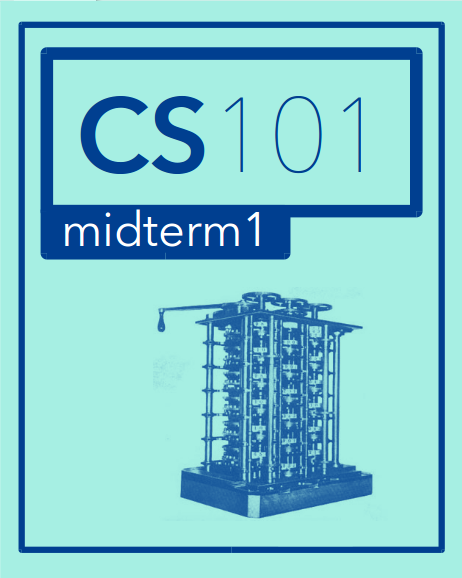
\includegraphics[width=2in]{../img/midterm1-header.png}
\end{center}

\bigskip
\noindent
\begin{itemize}
\item \textbf{Be sure to enter your \underline{NetID} and \underline{the code below} on your Scantron}.
\item Do not turn this page until instructed to do so.
\item There are 30 questions, worth 1 point each.
\item Each question has only \textbf{one} correct answer.
\item You must not communicate with other students during this test.
\item No books, notes, or electronic devices are permitted.
\item This is a 60-minute exam.
\item There are several different versions of this exam.
\end{itemize}

\bigskip\bigskip
\noindent
\textbf{\Large 1. Fill in your information:}

\bigskip
{\Large\bf
\begin{tabular}{ll}
Full Name: & \underbar{\hskip 8cm} \\[0.5em]
UIN (Student Number): & \underbar{\hskip 8cm} \\[0.5em]
NetID: & \underbar{\hskip 8cm}
\end{tabular}
}

\bigskip
\bigskip
\noindent
\textbf{\Large 2. Fill in the following answers on the Scantron form:}

%%%%%%%%%%%%%%%%%%%%%%%%%%%%%%%%%%%%%%%%%%%%%%%%%%%%%%%%%
%%%%%%%%%%%%%%%%%%%%%%%%%%%%%%%%%%%%%%%%%%%%%%%%%%%%%%%%%

\begin{enumerate}
\item[92.] D
\item[93.] C
\item[94.] B
\item[95.] E
\item[96.] C
\end{enumerate}

\newpage

% Zone 1


%%%%%%%%%%%%%%%%%%%%%%%%%%%%%%%%%%%%%%%%%%%%%%%%%%%%%%%%%



\newpage
\noindent
1. (1 point)
Consider the following program:
\begin{verbatim}
x=0
for i in range(2,7):
    if i%3==0:
        x+=3
    elif i%2==0:
        x+=2
    else:
        x+=1
\end{verbatim}
What is the \textbf{value} of \texttt{x} after this program is executed?


\begin{enumerate}
\item[(A)]
\begin{verbatim}10\end{verbatim}

\item[(B)]
\begin{verbatim}13\end{verbatim}

\item[(C)]
\begin{verbatim}14\end{verbatim}

\item[(D)]
\begin{verbatim}12\end{verbatim}

\item[(E)] $\bigstar$ 
\begin{verbatim}11\end{verbatim}

\end{enumerate}

\vspace*{2em}
\hrule
\vspace{2em}

\noindent {\bf Solution.} 
\vspace{2em}
\hrule height 2pt


\newpage
\noindent
2. (1 point)
Consider the following program.
\begin{verbatim}
s="BBCAA"
x=0
y=len(s)-1
while s[x]!=s[y] and x<len(s):
    x+=1
    y-=1
\end{verbatim}
After it is run, what is the final \textbf{value} of \texttt{x}?


\begin{enumerate}
\item[(A)]
\begin{verbatim}1\end{verbatim}

\item[(B)]
\begin{verbatim}4\end{verbatim}

\item[(C)] $\bigstar$ 
\begin{verbatim}2\end{verbatim}

\item[(D)]
\begin{verbatim}0\end{verbatim}

\item[(E)]
\begin{verbatim}3\end{verbatim}

\end{enumerate}

\vspace*{2em}
\hrule
\vspace{2em}

\noindent {\bf Solution.} 
\vspace{2em}
\hrule height 2pt


\newpage
\noindent
3. (1 point)
What is the result of the following expression?
\begin{verbatim}
[ 1, 2, 3 ] * 3.0
\end{verbatim}


\begin{enumerate}
\item[(A)] $\bigstar$ 
\begin{verbatim}[1, 2, 3, 1, 2, 3, 1, 2, 3]\end{verbatim}

\item[(B)]
\begin{verbatim}[3.0, 6.0, 9.0]\end{verbatim}

\item[(C)]
\begin{verbatim}[3, 6, 9]\end{verbatim}

\item[(D)]
\begin{verbatim}[1.0, 2.0, 3.0, 1.0, 2.0, 3.0, 1.0, 2.0, 3.0]\end{verbatim}

\item[(E)]
\begin{verbatim}None of the above.\end{verbatim}

\end{enumerate}

\vspace*{2em}
\hrule
\vspace{2em}

\noindent {\bf Solution.} 
\vspace{2em}
\hrule height 2pt


\newpage
\noindent
4. (1 point)
Consider the following program:
\begin{verbatim}
x=3
a=7
if (a%3)==2:
    x=x**2
elif(a%3)==1:
    x=x**1
else:
    x=x**0
\end{verbatim}
What is the \textbf{value} of \texttt{x} after this program is executed?


\begin{enumerate}
\item[(A)]
\begin{verbatim}9\end{verbatim}

\item[(B)]
\begin{verbatim}7\end{verbatim}

\item[(C)]
\begin{verbatim}1\end{verbatim}

\item[(D)]
None of the other answers are correct.

\item[(E)] $\bigstar$ 
\begin{verbatim}3\end{verbatim}

\end{enumerate}

\vspace*{2em}
\hrule
\vspace{2em}

\noindent {\bf Solution.} 
\vspace{2em}
\hrule height 2pt


\newpage
\noindent
5. (1 point)
Consider the following program:
\begin{verbatim}
def fix(s):
    a=list(s)
    a.sort()
    return ''.join(a)

x=["one","two","eleven","twelve"]
s1=fix(x[0]+x[-1])
s2=fix(x[1]+x[-2])

if s1<s2:
    x.sort()
elif s1>s2:
    x.reverse()
else:
    x.append("six")
\end{verbatim}
What is the \textbf{value} of \texttt{x} after this program is executed?


\begin{enumerate}
\item[(A)]
\begin{verbatim}['eleven', 'one', 'twelve', 'two']\end{verbatim}

\item[(B)]
\begin{verbatim}['twelve', 'eleven', 'two', 'one']\end{verbatim}

\item[(C)]
\begin{verbatim}['two', 'twelve', 'one', 'eleven', 'six']\end{verbatim}

\item[(D)]
\begin{verbatim}['one', 'two', 'eleven', 'twelve']\end{verbatim}

\item[(E)] $\bigstar$ 
\begin{verbatim}['one', 'two', 'eleven', 'twelve', 'six']\end{verbatim}

\end{enumerate}

\vspace*{2em}
\hrule
\vspace{2em}

\noindent {\bf Solution.} 
\vspace{2em}
\hrule height 2pt


\newpage
\noindent
6. (1 point)
Consider the following program.
\begin{verbatim}
x=[]
for j in range(0,5):
    if (j%4)==0:
        x.append("-")
    if (j%5)==0:
        x.append("*")
\end{verbatim}
After it is run, what is the final \textbf{value} of \texttt{x}?


\begin{enumerate}
\item[(A)]
\begin{verbatim}["-","*","*"]\end{verbatim}

\item[(B)]
\begin{verbatim}["-","-","*"]\end{verbatim}

\item[(C)] $\bigstar$ 
\begin{verbatim}["-","*","-"]\end{verbatim}

\item[(D)]
\begin{verbatim}["-","*"]\end{verbatim}

\item[(E)]
None of the other answers are correct.

\end{enumerate}

\vspace*{2em}
\hrule
\vspace{2em}

\noindent {\bf Solution.} 
\vspace{2em}
\hrule height 2pt


\newpage
\noindent
7. (1 point)
Consider the following program:
\begin{verbatim}
x=[1,2,3,4,5,6,7,8,9]
x=x[2:-2]
i=1
while i < 3:
    x[i]+=1
    i+=1
\end{verbatim}
What is the \textbf{value} of \texttt{x} after this program is executed?


\begin{enumerate}
\item[(A)] $\bigstar$ 
\begin{verbatim}[3, 5, 6, 6, 7]\end{verbatim}

\item[(B)]
\begin{verbatim}[3, 5, 6, 6]\end{verbatim}

\item[(C)]
\begin{verbatim}[2, 4, 5, 6, 6, 7]\end{verbatim}

\item[(D)]
\begin{verbatim}[3, 5, 6, 6, 7, 8]\end{verbatim}

\item[(E)]
\begin{verbatim}[2, 4, 5, 5, 6, 7]\end{verbatim}

\end{enumerate}

\vspace*{2em}
\hrule
\vspace{2em}

\noindent {\bf Solution.} 
\vspace{2em}
\hrule height 2pt


\newpage
\noindent
8. (1 point)
Consider the following program:
\begin{verbatim}
s="Hobbes"
i=0
x=-1
while i<len(s):
    if s[i]=='b':
        x=i
    i+=1
\end{verbatim}
What is the \textbf{value} of \texttt{x} after this program is executed?


\begin{enumerate}
\item[(A)]
\begin{verbatim}4\end{verbatim}

\item[(B)]
\begin{verbatim}5\end{verbatim}

\item[(C)] $\bigstar$ 
\begin{verbatim}3\end{verbatim}

\item[(D)]
\begin{verbatim}-1\end{verbatim}

\item[(E)]
\begin{verbatim}2\end{verbatim}

\end{enumerate}

\vspace*{2em}
\hrule
\vspace{2em}

\noindent {\bf Solution.} 
\vspace{2em}
\hrule height 2pt


\newpage
\noindent
9. (1 point)
Evaluate the following expression:
\begin{verbatim}
len("ABCDE"[1:4])
\end{verbatim}
What value is produced?


\begin{enumerate}
\item[(A)]
1

\item[(B)] $\bigstar$ 
3

\item[(C)]
4

\item[(D)]
5

\end{enumerate}

\vspace*{2em}
\hrule
\vspace{2em}

\noindent {\bf Solution.} 
\vspace{2em}
\hrule height 2pt


\newpage
\noindent
10. (1 point)
Consider the following program.
\begin{verbatim}
kay = 2
wart = 3

def knight(kay,wart):
    wart += 2
    kay += 3
    return wart + kay

wart = knight(kay, kay) + knight(wart, wart)
\end{verbatim}
After it is run, what is the final \textbf{value} of \texttt{wart}?


\begin{enumerate}
\item[(A)]
\begin{verbatim}3\end{verbatim}

\item[(B)]
\begin{verbatim}2\end{verbatim}

\item[(C)]
\begin{verbatim}5\end{verbatim}

\item[(D)] $\bigstar$ 
None of the other answers are correct.

\end{enumerate}

\vspace*{2em}
\hrule
\vspace{2em}

\noindent {\bf Solution.} 
\vspace{2em}
\hrule height 2pt


\newpage
\noindent
11. (1 point)
Consider the following program:
\begin{verbatim}
x=str(1.2)*2
\end{verbatim}
What is the \textbf{value} of \texttt{x} after this program is executed?


\begin{enumerate}
\item[(A)] $\bigstar$ 
\begin{verbatim}"1.21.2"\end{verbatim}

\item[(B)]
None of the other answers are correct.

\item[(C)]
\begin{verbatim}"1.2*2"\end{verbatim}

\item[(D)]
\begin{verbatim}2.4\end{verbatim}

\item[(E)]
\begin{verbatim}"2.4"\end{verbatim}

\end{enumerate}

\vspace*{2em}
\hrule
\vspace{2em}

\noindent {\bf Solution.} 
\vspace{2em}
\hrule height 2pt


\newpage
\noindent
12. (1 point)
Consider the following program:
\begin{verbatim}
a=["merlin","sir agravaine","king pellinore"]
b=[ ]
for i in range(0,3):
    b.append(a[0-i].title())
\end{verbatim}
What is the \textbf{value} of b after this program is executed?


\begin{enumerate}
\item[(A)]
\begin{verbatim}['Sir Agravaine', 'King Pellinore']\end{verbatim}

\item[(B)]
\begin{verbatim}['King Pellinore', 'Sir Agravaine', 'Merlin']\end{verbatim}

\item[(C)] $\bigstar$ 
\begin{verbatim}['Merlin', 'King Pellinore', 'Sir Agravaine']\end{verbatim}

\item[(D)]
\begin{verbatim}['King Pellinore', 'Sir Agravaine']\end{verbatim}

\item[(E)]
\begin{verbatim}[ ]\end{verbatim}

\end{enumerate}

\vspace*{2em}
\hrule
\vspace{2em}

\noindent {\bf Solution.} 
\vspace{2em}
\hrule height 2pt


\newpage
\noindent
13. (1 point)
Consider the following incomplete Python program.
\begin{verbatim}
s="".join(["1","0","2","1"])
x=0
for i in range(len(s)-1):
    x+=int(???)
\end{verbatim}
What should replace the three question marks so the resulting value of \texttt{x} is 33?


\begin{enumerate}
\item[(A)]
\begin{verbatim}s[i+1:i+2]\end{verbatim}

\item[(B)]
\begin{verbatim}s[i:i-1]\end{verbatim}

\item[(C)] $\bigstar$ 
\begin{verbatim}s[i:i+2]\end{verbatim}

\item[(D)]
\begin{verbatim}s[i:i+1]\end{verbatim}

\end{enumerate}

\vspace*{2em}
\hrule
\vspace{2em}

\noindent {\bf Solution.} 
\vspace{2em}
\hrule height 2pt


\newpage
\noindent
14. (1 point)
Consider the following program:
\begin{verbatim}
s="-B-O-R-S-"
x=s.split("-")[2:-2]
\end{verbatim}
What is the \textbf{value} of \texttt{x} after this program is executed?


\begin{enumerate}
\item[(A)]
\begin{verbatim}''\end{verbatim}

\item[(B)] $\bigstar$ 
\begin{verbatim}['O', 'R']\end{verbatim}

\item[(C)]
\begin{verbatim}False\end{verbatim}

\item[(D)]
\begin{verbatim}None\end{verbatim}

\item[(E)]
\begin{verbatim}'ORS'\end{verbatim}

\end{enumerate}

\vspace*{2em}
\hrule
\vspace{2em}

\noindent {\bf Solution.} 
\vspace{2em}
\hrule height 2pt


\newpage
\noindent
15. (1 point)
Consider the following program:
\begin{verbatim}
x=[1,2,3]
def f(a):
    s=""
    a.append(4)
    for i in a:
        s+=str(i)
    return s

x.append(f(x))
\end{verbatim}
What is the \textbf{value} of \texttt{x} after this program is executed?


\begin{enumerate}
\item[(A)]
\begin{verbatim}[1, 2, 3, '123']\end{verbatim}

\item[(B)] $\bigstar$ 
\begin{verbatim}[1, 2, 3, 4, '1234']\end{verbatim}

\item[(C)]
\begin{verbatim}[1, 2, 3, '1234']\end{verbatim}

\item[(D)]
\begin{verbatim}[1, 2, 3]\end{verbatim}

\item[(E)]
\begin{verbatim}[1, 2, 3, 10]\end{verbatim}

\end{enumerate}

\vspace*{2em}
\hrule
\vspace{2em}

\noindent {\bf Solution.} 
\vspace{2em}
\hrule height 2pt


\newpage
\noindent
16. (1 point)
How can the following mathematical equation be implemented as a Python expression? Assume \verb|a|, \verb|b|, and \verb|sin| have already been defined.
$$a \sin(a^b - b)$$


\begin{enumerate}
\item[(A)]
\begin{verbatim}a*sin(b^a - b)\end{verbatim}

\item[(B)] $\bigstar$ 
\begin{verbatim}a*sin(a**b - b)\end{verbatim}

\item[(C)]
\begin{verbatim}a sin(a**b - b)\end{verbatim}

\item[(D)]
None of the other answers are correct.

\item[(E)]
\begin{verbatim}a*sin(a^b - b)\end{verbatim}

\end{enumerate}

\vspace*{2em}
\hrule
\vspace{2em}

\noindent {\bf Solution.} 
\vspace{2em}
\hrule height 2pt


\newpage
\noindent
17. (1 point)
Consider the following program:
\begin{verbatim}
x="KING ARTHUR-MORGANA LEFAY-SIR BEDIVERE".split("-")
y=x[:]
y.reverse()
\end{verbatim}
What is the \textbf{value} of \texttt{x} after this program is executed?


\begin{enumerate}
\item[(A)]
\begin{verbatim}['BEDIVERE', 'LEFAY-SIR', 'ARTHUR-MORGANA', 'KING']\end{verbatim}

\item[(B)] $\bigstar$ 
\begin{verbatim}['KING ARTHUR', 'MORGANA LEFAY', 'SIR BEDIVERE']\end{verbatim}

\item[(C)]
\begin{verbatim}None\end{verbatim}

\item[(D)]
\begin{verbatim}['SIR BEDIVERE', 'MORGANA LEFAY', 'KING ARTHUR']\end{verbatim}

\item[(E)]
\begin{verbatim}['KING', 'ARTHUR-MORGANA', 'LEFAY-SIR', 'BEDIVERE']\end{verbatim}

\end{enumerate}

\vspace*{2em}
\hrule
\vspace{2em}

\noindent {\bf Solution.} 
\vspace{2em}
\hrule height 2pt


\newpage
\noindent
18. (1 point)
Consider the following program:
\begin{verbatim}
pi="3.14159"
e="2.71828"
x=pi*len(e)+pi
\end{verbatim}
What is the \textbf{type} of \texttt{x} after this program is executed?


\begin{enumerate}
\item[(A)] $\bigstar$ 
\begin{verbatim}String\end{verbatim}

\item[(B)]
\begin{verbatim}Integer\end{verbatim}

\item[(C)]
\begin{verbatim}None\end{verbatim}

\item[(D)]
\begin{verbatim}Float\end{verbatim}

\item[(E)]
\begin{verbatim}Boolean\end{verbatim}

\end{enumerate}

\vspace*{2em}
\hrule
\vspace{2em}

\noindent {\bf Solution.} 
\vspace{2em}
\hrule height 2pt


\newpage
\noindent
19. (1 point)
Consider the following program.
\begin{verbatim}
x=0
i=1
while(i*i)<=9:
    x=x+(i*i)
    i=i+1
\end{verbatim}
After it is run, what is the final \textbf{value} of \texttt{x}?


\begin{enumerate}
\item[(A)]
\begin{verbatim}5\end{verbatim}

\item[(B)]
\begin{verbatim}30\end{verbatim}

\item[(C)]
\begin{verbatim}3\end{verbatim}

\item[(D)]
\begin{verbatim}4\end{verbatim}

\item[(E)] $\bigstar$ 
\begin{verbatim}14\end{verbatim}

\end{enumerate}

\vspace*{2em}
\hrule
\vspace{2em}

\noindent {\bf Solution.} 
\vspace{2em}
\hrule height 2pt


\newpage
\noindent
20. (1 point)
Consider the following incomplete function.
\begin{verbatim}
def isdivisible(m,n):
    if ???:
        return False
    else:
        return True
\end{verbatim}
The function is intended to return True if the input parameter m is evenly divisible by the parameter n and False otherwise. For example, \verb|isdivisible(4,2)| should return \verb|True|, but \verb|isdivisible(5,3)| should return \verb|False|. What should replace the three question marks to complete the function?


\begin{enumerate}
\item[(A)]
\begin{verbatim}(n % m) == 0 \end{verbatim}

\item[(B)] $\bigstar$ 
\begin{verbatim}(m % n) != 0 \end{verbatim}

\item[(C)]
\begin{verbatim}(n // m) == 0 \end{verbatim}

\item[(D)]
\begin{verbatim}(m // n) != 0 \end{verbatim}

\end{enumerate}

\vspace*{2em}
\hrule
\vspace{2em}

\noindent {\bf Solution.} 
\vspace{2em}
\hrule height 2pt


\newpage
\noindent
21. (1 point)
Consider the following program:
\begin{verbatim}
a=3
b=4
if a==3:
    b=a
elif a==4:
    a=5
else:
    a=b
\end{verbatim}
What is the \textbf{value} of a after this program is executed?


\begin{enumerate}
\item[(A)]
\begin{verbatim}5\end{verbatim}

\item[(B)]
None of the other answers are correct.

\item[(C)]
\begin{verbatim}4\end{verbatim}

\item[(D)]
\begin{verbatim}7\end{verbatim}

\item[(E)] $\bigstar$ 
\begin{verbatim}3\end{verbatim}

\end{enumerate}

\vspace*{2em}
\hrule
\vspace{2em}

\noindent {\bf Solution.} 
\vspace{2em}
\hrule height 2pt


\newpage
\noindent
22. (1 point)
Consider the following program.
\begin{verbatim}
def artificing(s):
    return s*2
    return s+"%i" % 2
    return s

s=artificing("MERLIN")
\end{verbatim}
After it is run, what is the final \textbf{value} of s?


\begin{enumerate}
\item[(A)] $\bigstar$ 
\begin{verbatim}"MERLINMERLIN"\end{verbatim}

\item[(B)]
\begin{verbatim}"MERLIN2"\end{verbatim}

\item[(C)]
\begin{verbatim}12\end{verbatim}

\item[(D)]
\begin{verbatim}"MERLIN"\end{verbatim}

\item[(E)]
\begin{verbatim}None\end{verbatim}

\end{enumerate}

\vspace*{2em}
\hrule
\vspace{2em}

\noindent {\bf Solution.} 
\vspace{2em}
\hrule height 2pt


\newpage
\noindent
23. (1 point)
For this problem, you should compose a function which accomplishes a given task using the available code blocks arranged in the correct functional order.  \emph{We ignore indentation for this problem.}

\texttt{find\_max} should accept a \texttt{list} and return the value of the maximum item in the \texttt{list}.  (\texttt{None} is always the lowest value in any numeric comparison, so you may use it as an initializer.)

\begin{verbatim}
def find_max(my_list):
\end{verbatim}

\begin{enumerate}[1]
\item \texttt{max\_val = i}
\item \texttt{max\_val = None}
\item \texttt{for i in range(len(my\_list)):}
\item \texttt{if i > max\_val:}
\item \texttt{max\_val = my\_list[i]}
\item \texttt{return max\_val}
\item \texttt{for i in range(my\_list):}
\item \texttt{if my\_list[i] > max\_val:}
\item \texttt{print(max\_val)}
\end{enumerate}



\begin{enumerate}
\item[(A)]
2, 7, 4, 5, 6

\item[(B)]
2, 3, 8, 1, 6

\item[(C)] $\bigstar$ 
2, 3, 8, 5, 6

\item[(D)]
3, 2, 8, 5, 9

\item[(E)]
2, 3, 4, 1, 6

\end{enumerate}

\vspace*{2em}
\hrule
\vspace{2em}

\noindent {\bf Solution.} 
\vspace{2em}
\hrule height 2pt


\newpage
\noindent
24. (1 point)
Evaluate the following expression:
\begin{verbatim}
[1,2]+[len("3")]
\end{verbatim}
What value is produced?


\begin{enumerate}
\item[(A)]
\begin{verbatim}[1,2,"3"]\end{verbatim}

\item[(B)]
\begin{verbatim}[1,2,1,2,1,2]\end{verbatim}

\item[(C)] $\bigstar$ 
\begin{verbatim}[1,2,1]\end{verbatim}

\item[(D)]
\begin{verbatim}[1,2,3]\end{verbatim}

\end{enumerate}

\vspace*{2em}
\hrule
\vspace{2em}

\noindent {\bf Solution.} 
\vspace{2em}
\hrule height 2pt


\newpage
\noindent
25. (1 point)
Consider the following program:
\begin{verbatim}
i=3
x=2
while i < 7:
    x+=i
    i+=2
\end{verbatim}
What is the \textbf{value} of \texttt{x} after this program is executed?


\begin{enumerate}
\item[(A)]
\begin{verbatim}13\end{verbatim}

\item[(B)]
\begin{verbatim}14\end{verbatim}

\item[(C)]
\begin{verbatim}11\end{verbatim}

\item[(D)] $\bigstar$ 
\begin{verbatim}10\end{verbatim}

\item[(E)]
\begin{verbatim}12\end{verbatim}

\end{enumerate}

\vspace*{2em}
\hrule
\vspace{2em}

\noindent {\bf Solution.} 
\vspace{2em}
\hrule height 2pt


\newpage
\noindent
26. (1 point)
Consider the following incomplete program.
\begin{verbatim}
sum=0
???:
    sum=sum+i

\end{verbatim}
The program is intended to sum all of the integers between 1 and 100 (inclusive). What should replace the three question marks to complete the program?


\begin{enumerate}
\item[(A)] $\bigstar$ 
\begin{verbatim}for i in range(1,101) \end{verbatim}

\item[(B)]
\begin{verbatim}while i<=100 \end{verbatim}

\item[(C)]
\begin{verbatim}while i in range(100)\end{verbatim}

\item[(D)]
\begin{verbatim}for i in range(0,100)\end{verbatim}

\end{enumerate}

\vspace*{2em}
\hrule
\vspace{2em}

\noindent {\bf Solution.} 
\vspace{2em}
\hrule height 2pt


\newpage
\noindent
27. (1 point)
Consider the following program:
\begin{verbatim}
a=["A","C","C","I","O"]
a.sort()
a[0]=a[-1]
x=""
for e in a:
    x=x+e
\end{verbatim}
What is the \textbf{value} of \texttt{x} after this program is executed?


\begin{enumerate}
\item[(A)]
\begin{verbatim}"ICCOI"\end{verbatim}

\item[(B)] $\bigstar$ 
\begin{verbatim}"OCCIO"\end{verbatim}

\item[(C)]
None of the other answers are correct.

\item[(D)]
\begin{verbatim}"ACCOA"\end{verbatim}

\item[(E)]
\begin{verbatim}"ACCIA"\end{verbatim}

\end{enumerate}

\vspace*{2em}
\hrule
\vspace{2em}

\noindent {\bf Solution.} 
\vspace{2em}
\hrule height 2pt


\newpage
\noindent
28. (1 point)
Consider the following Python program.
\begin{verbatim}
e=[1,3,5,7,9,11]
d=[0,0,0]
for i in range(0,len(e)):
    d[i%3]+=e[i]
x=d[1]
\end{verbatim}
After it is run, what is the final \textbf{value} of \texttt{x}?


\begin{enumerate}
\item[(A)]
\begin{verbatim}16\end{verbatim}

\item[(B)] $\bigstar$ 
\begin{verbatim}12\end{verbatim}

\item[(C)]
\begin{verbatim}3\end{verbatim}

\item[(D)]
\begin{verbatim}0\end{verbatim}

\item[(E)]
\begin{verbatim}8\end{verbatim}

\end{enumerate}

\vspace*{2em}
\hrule
\vspace{2em}

\noindent {\bf Solution.} 
\vspace{2em}
\hrule height 2pt


\newpage
\noindent
29. (1 point)
Consider the following program:
\begin{verbatim}
s="TRIS %i"
t="ISEU"
x=s % len(t)
\end{verbatim}
What is the \textbf{type} of \texttt{x} after this program is executed?


\begin{enumerate}
\item[(A)]
\begin{verbatim}Boolean\end{verbatim}

\item[(B)]
\begin{verbatim}Float\end{verbatim}

\item[(C)] $\bigstar$ 
\begin{verbatim}String\end{verbatim}

\item[(D)]
\begin{verbatim}None\end{verbatim}

\item[(E)]
\begin{verbatim}Integer\end{verbatim}

\end{enumerate}

\vspace*{2em}
\hrule
\vspace{2em}

\noindent {\bf Solution.} 
\vspace{2em}
\hrule height 2pt


\newpage
\noindent
30. (1 point)
Consider the following program:
\begin{verbatim}
s="ECTOR"
t="GAWAIN"
x=len(str(s.isupper()))-t.find("A")
\end{verbatim}
What is the \textbf{type} of \texttt{x} after this program is executed?


\begin{enumerate}
\item[(A)]
\begin{verbatim}Boolean\end{verbatim}

\item[(B)]
\begin{verbatim}String\end{verbatim}

\item[(C)]
\begin{verbatim}None\end{verbatim}

\item[(D)] $\bigstar$ 
\begin{verbatim}Integer\end{verbatim}

\item[(E)]
\begin{verbatim}Float\end{verbatim}

\end{enumerate}

\vspace*{2em}
\hrule
\vspace{2em}

\noindent {\bf Solution.} 
\vspace{2em}
\hrule height 2pt

%%%%%%%%%%%%%%%%%%%%%%%%%%%%%%%%%%%%%%%%%%%%%%%%%%%%%%%%%%%%%%%%%%%%%%
%%%%%%%%%%%%%%%%%%%%%%%%%%%%%%%%%%%%%%%%%%%%%%%%%%%%%%%%%%%%%%%%%%%%%%
%%%%%%%%%%%%%%%%%%%%%%%%%%%%%%%%%%%%%%%%%%%%%%%%%%%%%%%%%%%%%%%%%%%%%%
%%%%%%%%%%%%%%%%%%%%%%%%%%%%%%%%%%%%%%%%%%%%%%%%%%%%%%%%%%%%%%%%%%%%%%
% Exam number 40

\message{Exam 40/50}
\cleardoublepage
\setcounter{page}{1}


\begin{center}
%\textbf{\Large CS 101 Midterm \#1}
%
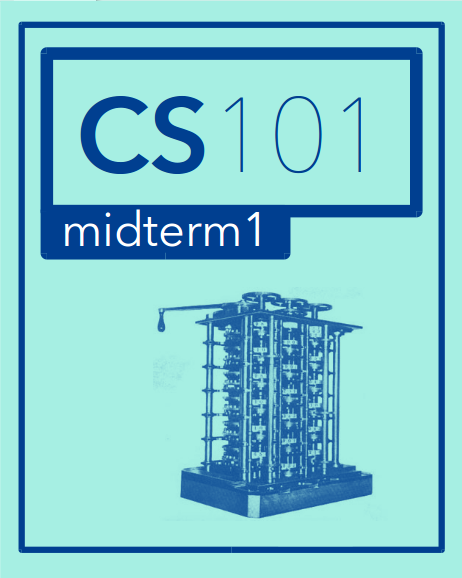
\includegraphics[width=2in]{../img/midterm1-header.png}
\end{center}

\bigskip
\noindent
\begin{itemize}
\item \textbf{Be sure to enter your \underline{NetID} and \underline{the code below} on your Scantron}.
\item Do not turn this page until instructed to do so.
\item There are 30 questions, worth 1 point each.
\item Each question has only \textbf{one} correct answer.
\item You must not communicate with other students during this test.
\item No books, notes, or electronic devices are permitted.
\item This is a 60-minute exam.
\item There are several different versions of this exam.
\end{itemize}

\bigskip\bigskip
\noindent
\textbf{\Large 1. Fill in your information:}

\bigskip
{\Large\bf
\begin{tabular}{ll}
Full Name: & \underbar{\hskip 8cm} \\[0.5em]
UIN (Student Number): & \underbar{\hskip 8cm} \\[0.5em]
NetID: & \underbar{\hskip 8cm}
\end{tabular}
}

\bigskip
\bigskip
\noindent
\textbf{\Large 2. Fill in the following answers on the Scantron form:}

%%%%%%%%%%%%%%%%%%%%%%%%%%%%%%%%%%%%%%%%%%%%%%%%%%%%%%%%%
%%%%%%%%%%%%%%%%%%%%%%%%%%%%%%%%%%%%%%%%%%%%%%%%%%%%%%%%%

\begin{enumerate}
\item[92.] E
\item[93.] C
\item[94.] B
\item[95.] A
\item[96.] D
\end{enumerate}

\newpage

% Zone 1


%%%%%%%%%%%%%%%%%%%%%%%%%%%%%%%%%%%%%%%%%%%%%%%%%%%%%%%%%



\newpage
\noindent
1. (1 point)
Consider the following program:
\begin{verbatim}
a=["S","T","U","P","E","F","Y"]
a=a[0:4]
a.sort()
x=""
for e in a:
    x=e+x
\end{verbatim}
What is the \textbf{value} of \texttt{x} after this program is executed?


\begin{enumerate}
\item[(A)]
\begin{verbatim}"PUST"\end{verbatim}

\item[(B)] $\bigstar$ 
\begin{verbatim}"UTSP"\end{verbatim}

\item[(C)]
\begin{verbatim}"PSTU"\end{verbatim}

\item[(D)]
\begin{verbatim}"STUP"\end{verbatim}

\item[(E)]
None of the other answers are correct.

\end{enumerate}

\vspace*{2em}
\hrule
\vspace{2em}

\noindent {\bf Solution.} 
\vspace{2em}
\hrule height 2pt


\newpage
\noindent
2. (1 point)
Consider the following program:
\begin{verbatim}
x=str(1.2)*2
\end{verbatim}
What is the \textbf{value} of \texttt{x} after this program is executed?


\begin{enumerate}
\item[(A)]
\begin{verbatim}"2.4"\end{verbatim}

\item[(B)]
\begin{verbatim}2.4\end{verbatim}

\item[(C)]
None of the other answers are correct.

\item[(D)]
\begin{verbatim}"1.2*2"\end{verbatim}

\item[(E)] $\bigstar$ 
\begin{verbatim}"1.21.2"\end{verbatim}

\end{enumerate}

\vspace*{2em}
\hrule
\vspace{2em}

\noindent {\bf Solution.} 
\vspace{2em}
\hrule height 2pt


\newpage
\noindent
3. (1 point)
Consider the following program:
\begin{verbatim}
s="TRIS %i"
t="ISEU"
x=len(s) % len(t[2:-1])
\end{verbatim}
What is the \textbf{type} of \texttt{x} after this program is executed?


\begin{enumerate}
\item[(A)]
\begin{verbatim}None\end{verbatim}

\item[(B)]
\begin{verbatim}Boolean\end{verbatim}

\item[(C)]
\begin{verbatim}String\end{verbatim}

\item[(D)]
\begin{verbatim}Float\end{verbatim}

\item[(E)] $\bigstar$ 
\begin{verbatim}Integer\end{verbatim}

\end{enumerate}

\vspace*{2em}
\hrule
\vspace{2em}

\noindent {\bf Solution.} 
\vspace{2em}
\hrule height 2pt


\newpage
\noindent
4. (1 point)
Consider the following program:
\begin{verbatim}
a=["merlin","sir agravaine","king pellinore"]
b=[ ]
for i in range(0,4):
    b.append(a[0-i].title())
\end{verbatim}
What is the \textbf{value} of b after this program is executed?


\begin{enumerate}
\item[(A)]
\begin{verbatim}['King Pellinore', 'Sir Agravaine', 'Merlin']\end{verbatim}

\item[(B)]
\begin{verbatim}['Merlin', 'King Pellinore', 'Sir Agravaine']\end{verbatim}

\item[(C)]
\begin{verbatim}['Merlin', 'Sir Agravaine', 'King Pellinore', 'Merlin']\end{verbatim}

\item[(D)] $\bigstar$ 
\begin{verbatim}['Merlin', 'King Pellinore', 'Sir Agravaine', 'Merlin']\end{verbatim}

\item[(E)]
\begin{verbatim}[ ]\end{verbatim}

\end{enumerate}

\vspace*{2em}
\hrule
\vspace{2em}

\noindent {\bf Solution.} 
\vspace{2em}
\hrule height 2pt


\newpage
\noindent
5. (1 point)
Consider the following program:
\begin{verbatim}
x=0
for i in range(2,8):
    if i%3==0:
        x+=3
    elif i%2==0:
        x+=2
    else:
        x+=1
\end{verbatim}
What is the \textbf{value} of \texttt{x} after this program is executed?


\begin{enumerate}
\item[(A)]
\begin{verbatim}13\end{verbatim}

\item[(B)]
\begin{verbatim}10\end{verbatim}

\item[(C)] $\bigstar$ 
\begin{verbatim}12\end{verbatim}

\item[(D)]
\begin{verbatim}14\end{verbatim}

\item[(E)]
\begin{verbatim}11\end{verbatim}

\end{enumerate}

\vspace*{2em}
\hrule
\vspace{2em}

\noindent {\bf Solution.} 
\vspace{2em}
\hrule height 2pt


\newpage
\noindent
6. (1 point)
Consider the following program:
\begin{verbatim}
x="KING ARTHUR-MORGANA LEFAY-SIR BEDIVERE".split("-")
y=x
x=y.reverse()
\end{verbatim}
What is the \textbf{value} of \texttt{x} after this program is executed?


\begin{enumerate}
\item[(A)]
\begin{verbatim}['KING', 'ARTHUR-MORGANA', 'LEFAY-SIR', 'BEDIVERE']\end{verbatim}

\item[(B)]
\begin{verbatim}['SIR BEDIVERE', 'MORGANA LEFAY', 'KING ARTHUR']\end{verbatim}

\item[(C)]
\begin{verbatim}['KING ARTHUR', 'MORGANA LEFAY', 'SIR BEDIVERE']\end{verbatim}

\item[(D)]
\begin{verbatim}['BEDIVERE', 'LEFAY-SIR', 'ARTHUR-MORGANA', 'KING']\end{verbatim}

\item[(E)] $\bigstar$ 
\begin{verbatim}None\end{verbatim}

\end{enumerate}

\vspace*{2em}
\hrule
\vspace{2em}

\noindent {\bf Solution.} 
\vspace{2em}
\hrule height 2pt


\newpage
\noindent
7. (1 point)
Consider the following program:
\begin{verbatim}
s="G+R+A+I+L"
x=s.split("+")[1:-2]
\end{verbatim}
What is the \textbf{value} of \texttt{x} after this program is executed?


\begin{enumerate}
\item[(A)]
\begin{verbatim}3\end{verbatim}

\item[(B)]
\begin{verbatim}False\end{verbatim}

\item[(C)]
\begin{verbatim}'RAI'\end{verbatim}

\item[(D)] $\bigstar$ 
\begin{verbatim}['R','A']\end{verbatim}

\item[(E)]
\begin{verbatim}None\end{verbatim}

\end{enumerate}

\vspace*{2em}
\hrule
\vspace{2em}

\noindent {\bf Solution.} 
\vspace{2em}
\hrule height 2pt


\newpage
\noindent
8. (1 point)
How can the following mathematical equation be implemented as a Python expression? Assume \verb|a|, \verb|b|, and \verb|sin| have already been defined.
$$a \sin(a^b - b)$$


\begin{enumerate}
\item[(A)]
\begin{verbatim}a*sin(a^b - b)\end{verbatim}

\item[(B)]
None of the other answers are correct.

\item[(C)]
\begin{verbatim}a sin(a**b - b)\end{verbatim}

\item[(D)]
\begin{verbatim}a*sin(b^a - b)\end{verbatim}

\item[(E)] $\bigstar$ 
\begin{verbatim}a*sin(a**b - b)\end{verbatim}

\end{enumerate}

\vspace*{2em}
\hrule
\vspace{2em}

\noindent {\bf Solution.} 
\vspace{2em}
\hrule height 2pt


\newpage
\noindent
9. (1 point)
Consider the following incomplete function.
\begin{verbatim}
def ismultiple(m,n):
    if ???:
        return False
    else:
        return True
\end{verbatim}
The function is intended to return True if the input parameter m is a multiple of parameter n and False otherwise. For example, \verb|ismultiple(4,2)| should return \verb|True|, but \verb|ismultiple(5,3)| should return \verb|False|. What should replace the three question marks to complete the function?


\begin{enumerate}
\item[(A)]
\begin{verbatim}(n // m) == 0 \end{verbatim}

\item[(B)]
\begin{verbatim}(n % m) == 0 \end{verbatim}

\item[(C)] $\bigstar$ 
\begin{verbatim}(m % n) != 0 \end{verbatim}

\item[(D)]
\begin{verbatim}(m // n) != 0 \end{verbatim}

\end{enumerate}

\vspace*{2em}
\hrule
\vspace{2em}

\noindent {\bf Solution.} 
\vspace{2em}
\hrule height 2pt


\newpage
\noindent
10. (1 point)
Consider the following Python program.
\begin{verbatim}
e=[1,3,5,7,9,11]
d=[0,0,0]
for i in range(0,len(e)):
    d[i%3]+=e[i]
x=d[1]
\end{verbatim}
After it is run, what is the final \textbf{value} of \texttt{x}?


\begin{enumerate}
\item[(A)] $\bigstar$ 
\begin{verbatim}12\end{verbatim}

\item[(B)]
\begin{verbatim}0\end{verbatim}

\item[(C)]
\begin{verbatim}16\end{verbatim}

\item[(D)]
\begin{verbatim}8\end{verbatim}

\item[(E)]
\begin{verbatim}3\end{verbatim}

\end{enumerate}

\vspace*{2em}
\hrule
\vspace{2em}

\noindent {\bf Solution.} 
\vspace{2em}
\hrule height 2pt


\newpage
\noindent
11. (1 point)
Consider the following program.
\begin{verbatim}
x=1
i=0
while(x*x)<=9:
    i=i+(x*x)
    x=x+1
\end{verbatim}
After it is run, what is the final \textbf{value} of \texttt{x}?


\begin{enumerate}
\item[(A)]
\begin{verbatim}30\end{verbatim}

\item[(B)] $\bigstar$ 
\begin{verbatim}4\end{verbatim}

\item[(C)]
\begin{verbatim}3\end{verbatim}

\item[(D)]
\begin{verbatim}14\end{verbatim}

\item[(E)]
\begin{verbatim}5\end{verbatim}

\end{enumerate}

\vspace*{2em}
\hrule
\vspace{2em}

\noindent {\bf Solution.} 
\vspace{2em}
\hrule height 2pt


\newpage
\noindent
12. (1 point)
Consider the following program:
\begin{verbatim}
x=[1,2,3]
def f(a):
    s=""
    a.append(4)
    for i in a:
        s+=str(i)
    return s

x.append(f(x))
\end{verbatim}
What is the \textbf{value} of \texttt{x} after this program is executed?


\begin{enumerate}
\item[(A)]
\begin{verbatim}[1, 2, 3, '1234']\end{verbatim}

\item[(B)]
\begin{verbatim}[1, 2, 3, '123']\end{verbatim}

\item[(C)]
\begin{verbatim}[1, 2, 3, 10]\end{verbatim}

\item[(D)] $\bigstar$ 
\begin{verbatim}[1, 2, 3, 4, '1234']\end{verbatim}

\item[(E)]
\begin{verbatim}[1, 2, 3]\end{verbatim}

\end{enumerate}

\vspace*{2em}
\hrule
\vspace{2em}

\noindent {\bf Solution.} 
\vspace{2em}
\hrule height 2pt


\newpage
\noindent
13. (1 point)
Consider the following program.
\begin{verbatim}
def artificing(s):
    return s+"%i" % 2
    return s*2
    return s

s=artificing("MERLIN")
\end{verbatim}
After it is run, what is the final \textbf{value} of s?


\begin{enumerate}
\item[(A)]
\begin{verbatim}0\end{verbatim}

\item[(B)]
\begin{verbatim}None\end{verbatim}

\item[(C)]
\begin{verbatim}"MERLIN%i"\end{verbatim}

\item[(D)] $\bigstar$ 
\begin{verbatim}"MERLIN2"\end{verbatim}

\item[(E)]
\begin{verbatim}"MERLINMERLIN"\end{verbatim}

\end{enumerate}

\vspace*{2em}
\hrule
\vspace{2em}

\noindent {\bf Solution.} 
\vspace{2em}
\hrule height 2pt


\newpage
\noindent
14. (1 point)
For this problem, you should compose a function which accomplishes a given task using the available code blocks arranged in the correct functional order.  \emph{We ignore indentation for this problem.}

\texttt{find\_max} should accept a \texttt{list} and return the value of the maximum item in the \texttt{list}.  (\texttt{None} is always the lowest value in any numeric comparison, so you may use it as an initializer.)

\begin{verbatim}
def find_max(my_list):
\end{verbatim}

\begin{enumerate}[1]
\item \texttt{max\_val = i}
\item \texttt{max\_val = None}
\item \texttt{for i in range(len(my\_list)):}
\item \texttt{if i > max\_val:}
\item \texttt{max\_val = my\_list[i]}
\item \texttt{return max\_val}
\item \texttt{for i in range(my\_list):}
\item \texttt{if my\_list[i] > max\_val:}
\item \texttt{print(max\_val)}
\end{enumerate}



\begin{enumerate}
\item[(A)]
3, 2, 8, 5, 9

\item[(B)]
2, 3, 8, 1, 6

\item[(C)]
2, 3, 4, 1, 6

\item[(D)]
2, 7, 4, 5, 6

\item[(E)] $\bigstar$ 
2, 3, 8, 5, 6

\end{enumerate}

\vspace*{2em}
\hrule
\vspace{2em}

\noindent {\bf Solution.} 
\vspace{2em}
\hrule height 2pt


\newpage
\noindent
15. (1 point)
Consider the following program.
\begin{verbatim}
s="BBCAA"
x=0
y=len(s)-1
while s[x]!=s[y] and x<len(s):
    x+=1
    y-=1
\end{verbatim}
After it is run, what is the final \textbf{value} of \texttt{x}?


\begin{enumerate}
\item[(A)]
\begin{verbatim}4\end{verbatim}

\item[(B)]
\begin{verbatim}1\end{verbatim}

\item[(C)]
\begin{verbatim}3\end{verbatim}

\item[(D)] $\bigstar$ 
\begin{verbatim}2\end{verbatim}

\item[(E)]
\begin{verbatim}0\end{verbatim}

\end{enumerate}

\vspace*{2em}
\hrule
\vspace{2em}

\noindent {\bf Solution.} 
\vspace{2em}
\hrule height 2pt


\newpage
\noindent
16. (1 point)
Consider the following incomplete program.
\begin{verbatim}
sum=0
for i in range(0,100):
    ???

\end{verbatim}
The program is intended to sum all of the integers between 1 and 100 (inclusive). What should replace the three question marks to complete the program?


\begin{enumerate}
\item[(A)]
\begin{verbatim}sum=sum+i \end{verbatim}

\item[(B)] $\bigstar$ 
\begin{verbatim}sum=sum+i+1 \end{verbatim}

\item[(C)]
\begin{verbatim}sum=sum+1\end{verbatim}

\item[(D)]
\begin{verbatim}sum+1=sum \end{verbatim}

\end{enumerate}

\vspace*{2em}
\hrule
\vspace{2em}

\noindent {\bf Solution.} 
\vspace{2em}
\hrule height 2pt


\newpage
\noindent
17. (1 point)
Consider the following program:
\begin{verbatim}
x=[2,3,4,5,6,7,8,9]
x=x[2:-2]
i=1
while i <= 3:
    x[i]+=1
    i+=1
\end{verbatim}
What is the \textbf{value} of \texttt{x} after this program is executed?


\begin{enumerate}
\item[(A)]
\begin{verbatim}[4, 6, 7]\end{verbatim}

\item[(B)]
\begin{verbatim}[2, 4, 6, 6]\end{verbatim}

\item[(C)]
\begin{verbatim}[4, 6, 7, 7]\end{verbatim}

\item[(D)] $\bigstar$ 
\begin{verbatim}[4, 6, 7, 8]\end{verbatim}

\item[(E)]
\begin{verbatim}[3, 4, 6, 7, 8]\end{verbatim}

\end{enumerate}

\vspace*{2em}
\hrule
\vspace{2em}

\noindent {\bf Solution.} 
\vspace{2em}
\hrule height 2pt


\newpage
\noindent
18. (1 point)
Consider the following program:
\begin{verbatim}
pi="3.14159"
e="2.71828"
x=(float(e)**float(pi)-float(pi)) == 20
\end{verbatim}
What is the \textbf{type} of \texttt{x} after this program is executed?


\begin{enumerate}
\item[(A)]
\begin{verbatim}Float\end{verbatim}

\item[(B)]
\begin{verbatim}Integer\end{verbatim}

\item[(C)]
\begin{verbatim}String\end{verbatim}

\item[(D)]
\begin{verbatim}None\end{verbatim}

\item[(E)] $\bigstar$ 
\begin{verbatim}Boolean\end{verbatim}

\end{enumerate}

\vspace*{2em}
\hrule
\vspace{2em}

\noindent {\bf Solution.} 
\vspace{2em}
\hrule height 2pt


\newpage
\noindent
19. (1 point)
Consider the following program.
\begin{verbatim}
x=[]
for j in range(0,5):
    if (j%2)==0:
        x.append("-")
    if (j%5)==0:
        x.append("*")
\end{verbatim}
After it is run, what is the final \textbf{value} of \texttt{x}?


\begin{enumerate}
\item[(A)]
\begin{verbatim}["-","*","-"]\end{verbatim}

\item[(B)]
\begin{verbatim}["*","-","*","*"]\end{verbatim}

\item[(C)] $\bigstar$ 
\begin{verbatim}["-","*","-","-"]\end{verbatim}

\item[(D)]
\begin{verbatim}["-","-","*"]\end{verbatim}

\item[(E)]
None of the other answers are correct.

\end{enumerate}

\vspace*{2em}
\hrule
\vspace{2em}

\noindent {\bf Solution.} 
\vspace{2em}
\hrule height 2pt


\newpage
\noindent
20. (1 point)
Evaluate the following expression:
\begin{verbatim}
[1,2]*len("3")
\end{verbatim}
What value is produced?


\begin{enumerate}
\item[(A)]
\begin{verbatim}[1,2,3]\end{verbatim}

\item[(B)]
\begin{verbatim}[1,2,1]\end{verbatim}

\item[(C)]
\begin{verbatim}[1,2,1,2,1,2]\end{verbatim}

\item[(D)] $\bigstar$ 
\begin{verbatim}[1,2]\end{verbatim}

\end{enumerate}

\vspace*{2em}
\hrule
\vspace{2em}

\noindent {\bf Solution.} 
\vspace{2em}
\hrule height 2pt


\newpage
\noindent
21. (1 point)
Consider the following program:
\begin{verbatim}
s="Calvin"
i=0
x=-1
while i<len(s):
    if s[i]=='b':
        x=i
    i+=1
\end{verbatim}
What is the \textbf{value} of \texttt{x} after this program is executed?


\begin{enumerate}
\item[(A)]
\begin{verbatim}5\end{verbatim}

\item[(B)]
\begin{verbatim}6\end{verbatim}

\item[(C)] $\bigstar$ 
\begin{verbatim}-1\end{verbatim}

\item[(D)]
\begin{verbatim}0\end{verbatim}

\item[(E)]
\begin{verbatim}3\end{verbatim}

\end{enumerate}

\vspace*{2em}
\hrule
\vspace{2em}

\noindent {\bf Solution.} 
\vspace{2em}
\hrule height 2pt


\newpage
\noindent
22. (1 point)
Consider the following incomplete Python program.
\begin{verbatim}
s="".join(["0","1","2","1"])
x=0
for i in range(len(s)-1):
    x+=int(???)
\end{verbatim}
What should replace the three question marks so the resulting value of \texttt{x} is 34?


\begin{enumerate}
\item[(A)]
\begin{verbatim}s[i:i-1]\end{verbatim}

\item[(B)]
\begin{verbatim}s[i+1:i+2]\end{verbatim}

\item[(C)] $\bigstar$ 
\begin{verbatim}s[i:i+2]\end{verbatim}

\item[(D)]
\begin{verbatim}s[i:i+1]\end{verbatim}

\end{enumerate}

\vspace*{2em}
\hrule
\vspace{2em}

\noindent {\bf Solution.} 
\vspace{2em}
\hrule height 2pt


\newpage
\noindent
23. (1 point)
Consider the following program:
\begin{verbatim}
a=3
b=4
if a!=b:
    a=b
elif a==4:
    a=5
else:
    b=a
\end{verbatim}
What is the \textbf{value} of a after this program is executed?


\begin{enumerate}
\item[(A)]
\begin{verbatim}3\end{verbatim}

\item[(B)]
\begin{verbatim}5\end{verbatim}

\item[(C)]
\begin{verbatim}7\end{verbatim}

\item[(D)] $\bigstar$ 
\begin{verbatim}4\end{verbatim}

\item[(E)]
None of the other answers are correct.

\end{enumerate}

\vspace*{2em}
\hrule
\vspace{2em}

\noindent {\bf Solution.} 
\vspace{2em}
\hrule height 2pt


\newpage
\noindent
24. (1 point)
Consider the following program:
\begin{verbatim}
i=3
x=2
while i < 7:
    x+=i
    i+=2
\end{verbatim}
What is the \textbf{value} of \texttt{x} after this program is executed?


\begin{enumerate}
\item[(A)] $\bigstar$ 
\begin{verbatim}10\end{verbatim}

\item[(B)]
\begin{verbatim}12\end{verbatim}

\item[(C)]
\begin{verbatim}14\end{verbatim}

\item[(D)]
\begin{verbatim}11\end{verbatim}

\item[(E)]
\begin{verbatim}13\end{verbatim}

\end{enumerate}

\vspace*{2em}
\hrule
\vspace{2em}

\noindent {\bf Solution.} 
\vspace{2em}
\hrule height 2pt


\newpage
\noindent
25. (1 point)
Evaluate the following expression:
\begin{verbatim}
len("ABCD"[0:3])
\end{verbatim}
What value is produced?


\begin{enumerate}
\item[(A)]
2

\item[(B)]
1

\item[(C)]
4

\item[(D)] $\bigstar$ 
3

\end{enumerate}

\vspace*{2em}
\hrule
\vspace{2em}

\noindent {\bf Solution.} 
\vspace{2em}
\hrule height 2pt


\newpage
\noindent
26. (1 point)
Consider the following program:
\begin{verbatim}
def fix(s):
    a=list(s)
    a.sort()
    return ''.join(a)

x=["one","two","eleven","twelve"]
s1=fix(x[0]+x[-1])
s2=fix(x[1]+x[-2])

if s1<s2:
    x.sort()
elif s1>s2:
    x.reverse()
else:
    x.append("six")
\end{verbatim}
What is the \textbf{value} of \texttt{x} after this program is executed?


\begin{enumerate}
\item[(A)]
\begin{verbatim}['eleven', 'one', 'twelve', 'two']\end{verbatim}

\item[(B)] $\bigstar$ 
\begin{verbatim}['one', 'two', 'eleven', 'twelve', 'six']\end{verbatim}

\item[(C)]
\begin{verbatim}['two', 'twelve', 'one', 'eleven', 'six']\end{verbatim}

\item[(D)]
\begin{verbatim}['twelve', 'eleven', 'two', 'one']\end{verbatim}

\item[(E)]
\begin{verbatim}['one', 'two', 'eleven', 'twelve']\end{verbatim}

\end{enumerate}

\vspace*{2em}
\hrule
\vspace{2em}

\noindent {\bf Solution.} 
\vspace{2em}
\hrule height 2pt


\newpage
\noindent
27. (1 point)
What is the result of the following expression?
\begin{verbatim}
[ 1, 2, 3 ] * 3.0
\end{verbatim}


\begin{enumerate}
\item[(A)] $\bigstar$ 
\begin{verbatim}[1, 2, 3, 1, 2, 3, 1, 2, 3]\end{verbatim}

\item[(B)]
\begin{verbatim}[1.0, 2.0, 3.0, 1.0, 2.0, 3.0, 1.0, 2.0, 3.0]\end{verbatim}

\item[(C)]
\begin{verbatim}[3.0, 6.0, 9.0]\end{verbatim}

\item[(D)]
\begin{verbatim}None of the above.\end{verbatim}

\item[(E)]
\begin{verbatim}[3, 6, 9]\end{verbatim}

\end{enumerate}

\vspace*{2em}
\hrule
\vspace{2em}

\noindent {\bf Solution.} 
\vspace{2em}
\hrule height 2pt


\newpage
\noindent
28. (1 point)
Consider the following program.
\begin{verbatim}
kay = 2
wart = 3

def knight(kay,wart):
    wart += 2
    kay += 3
    return wart + kay

kay = knight(wart, kay) + knight(kay, wart)
\end{verbatim}
After it is run, what is the final \textbf{value} of \texttt{kay}?


\begin{enumerate}
\item[(A)] $\bigstar$ 
None of the other answers are correct.

\item[(B)]
\begin{verbatim}5\end{verbatim}

\item[(C)]
\begin{verbatim}3\end{verbatim}

\item[(D)]
\begin{verbatim}2\end{verbatim}

\end{enumerate}

\vspace*{2em}
\hrule
\vspace{2em}

\noindent {\bf Solution.} 
\vspace{2em}
\hrule height 2pt


\newpage
\noindent
29. (1 point)
Consider the following program:
\begin{verbatim}
s="ECTOR"
t="GAWAIN"
x=(len(s)/(len(t)-1))+1
\end{verbatim}
What is the \textbf{type} of \texttt{x} after this program is executed?


\begin{enumerate}
\item[(A)]
\begin{verbatim}Boolean\end{verbatim}

\item[(B)]
\begin{verbatim}Integer\end{verbatim}

\item[(C)]
\begin{verbatim}String\end{verbatim}

\item[(D)] $\bigstar$ 
\begin{verbatim}Float\end{verbatim}

\item[(E)]
\begin{verbatim}None\end{verbatim}

\end{enumerate}

\vspace*{2em}
\hrule
\vspace{2em}

\noindent {\bf Solution.} 
\vspace{2em}
\hrule height 2pt


\newpage
\noindent
30. (1 point)
Consider the following program:
\begin{verbatim}
x=2
a=6
if (a%3)==2:
    x=x**3
elif(a%3)==1:
    x=x**2
else:
    x=x**1
\end{verbatim}
What is the \textbf{value} of \texttt{x} after this program is executed?


\begin{enumerate}
\item[(A)]
\begin{verbatim}16\end{verbatim}

\item[(B)]
None of the other answers are correct.

\item[(C)]
\begin{verbatim}8\end{verbatim}

\item[(D)]
\begin{verbatim}4\end{verbatim}

\item[(E)] $\bigstar$ 
\begin{verbatim}2\end{verbatim}

\end{enumerate}

\vspace*{2em}
\hrule
\vspace{2em}

\noindent {\bf Solution.} 
\vspace{2em}
\hrule height 2pt

%%%%%%%%%%%%%%%%%%%%%%%%%%%%%%%%%%%%%%%%%%%%%%%%%%%%%%%%%%%%%%%%%%%%%%
%%%%%%%%%%%%%%%%%%%%%%%%%%%%%%%%%%%%%%%%%%%%%%%%%%%%%%%%%%%%%%%%%%%%%%
%%%%%%%%%%%%%%%%%%%%%%%%%%%%%%%%%%%%%%%%%%%%%%%%%%%%%%%%%%%%%%%%%%%%%%
%%%%%%%%%%%%%%%%%%%%%%%%%%%%%%%%%%%%%%%%%%%%%%%%%%%%%%%%%%%%%%%%%%%%%%
% Exam number 41

\message{Exam 41/50}
\cleardoublepage
\setcounter{page}{1}


\begin{center}
%\textbf{\Large CS 101 Midterm \#1}
%
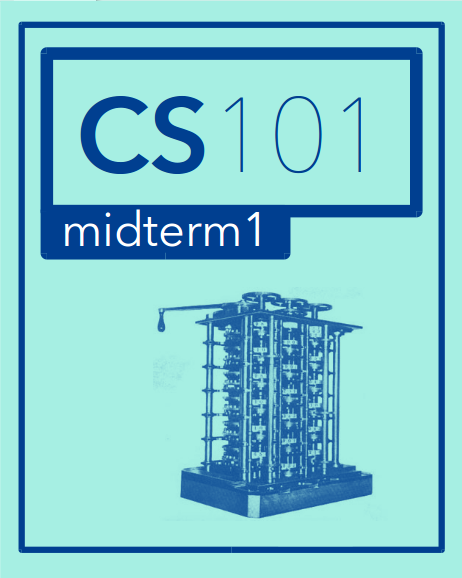
\includegraphics[width=2in]{../img/midterm1-header.png}
\end{center}

\bigskip
\noindent
\begin{itemize}
\item \textbf{Be sure to enter your \underline{NetID} and \underline{the code below} on your Scantron}.
\item Do not turn this page until instructed to do so.
\item There are 30 questions, worth 1 point each.
\item Each question has only \textbf{one} correct answer.
\item You must not communicate with other students during this test.
\item No books, notes, or electronic devices are permitted.
\item This is a 60-minute exam.
\item There are several different versions of this exam.
\end{itemize}

\bigskip\bigskip
\noindent
\textbf{\Large 1. Fill in your information:}

\bigskip
{\Large\bf
\begin{tabular}{ll}
Full Name: & \underbar{\hskip 8cm} \\[0.5em]
UIN (Student Number): & \underbar{\hskip 8cm} \\[0.5em]
NetID: & \underbar{\hskip 8cm}
\end{tabular}
}

\bigskip
\bigskip
\noindent
\textbf{\Large 2. Fill in the following answers on the Scantron form:}

%%%%%%%%%%%%%%%%%%%%%%%%%%%%%%%%%%%%%%%%%%%%%%%%%%%%%%%%%
%%%%%%%%%%%%%%%%%%%%%%%%%%%%%%%%%%%%%%%%%%%%%%%%%%%%%%%%%

\begin{enumerate}
\item[92.] A
\item[93.] D
\item[94.] B
\item[95.] C
\item[96.] B
\end{enumerate}

\newpage

% Zone 1


%%%%%%%%%%%%%%%%%%%%%%%%%%%%%%%%%%%%%%%%%%%%%%%%%%%%%%%%%



\newpage
\noindent
1. (1 point)
Consider the following Python program.
\begin{verbatim}
e=[1,3,5,7,9,11]
d=[0,0,0]
for i in range(0,len(e)):
    d[i%3]+=e[i]
x=d[2]
\end{verbatim}
After it is run, what is the final \textbf{value} of \texttt{x}?


\begin{enumerate}
\item[(A)] $\bigstar$ 
\begin{verbatim}16\end{verbatim}

\item[(B)]
\begin{verbatim}0\end{verbatim}

\item[(C)]
\begin{verbatim}7\end{verbatim}

\item[(D)]
\begin{verbatim}12\end{verbatim}

\item[(E)]
\begin{verbatim}8\end{verbatim}

\end{enumerate}

\vspace*{2em}
\hrule
\vspace{2em}

\noindent {\bf Solution.} 
\vspace{2em}
\hrule height 2pt


\newpage
\noindent
2. (1 point)
Consider the following program:
\begin{verbatim}
s="TRIS %i"
t="ISEU"
x=s % len(t)
\end{verbatim}
What is the \textbf{type} of \texttt{x} after this program is executed?


\begin{enumerate}
\item[(A)]
\begin{verbatim}None\end{verbatim}

\item[(B)] $\bigstar$ 
\begin{verbatim}String\end{verbatim}

\item[(C)]
\begin{verbatim}Integer\end{verbatim}

\item[(D)]
\begin{verbatim}Float\end{verbatim}

\item[(E)]
\begin{verbatim}Boolean\end{verbatim}

\end{enumerate}

\vspace*{2em}
\hrule
\vspace{2em}

\noindent {\bf Solution.} 
\vspace{2em}
\hrule height 2pt


\newpage
\noindent
3. (1 point)
Consider the following program:
\begin{verbatim}
i=2
x=3
while i < 7:
    x+=i
    i+=2
\end{verbatim}
What is the \textbf{value} of \texttt{x} after this program is executed?


\begin{enumerate}
\item[(A)]
\begin{verbatim}12\end{verbatim}

\item[(B)] $\bigstar$ 
\begin{verbatim}15\end{verbatim}

\item[(C)]
\begin{verbatim}11\end{verbatim}

\item[(D)]
\begin{verbatim}14\end{verbatim}

\item[(E)]
\begin{verbatim}13\end{verbatim}

\end{enumerate}

\vspace*{2em}
\hrule
\vspace{2em}

\noindent {\bf Solution.} 
\vspace{2em}
\hrule height 2pt


\newpage
\noindent
4. (1 point)
Evaluate the following expression:
\begin{verbatim}
[1,2]+[len("3")]
\end{verbatim}
What value is produced?


\begin{enumerate}
\item[(A)]
\begin{verbatim}[1,2,3]\end{verbatim}

\item[(B)]
\begin{verbatim}[1,2,1,2,1,2]\end{verbatim}

\item[(C)]
\begin{verbatim}[1,2,"3"]\end{verbatim}

\item[(D)] $\bigstar$ 
\begin{verbatim}[1,2,1]\end{verbatim}

\end{enumerate}

\vspace*{2em}
\hrule
\vspace{2em}

\noindent {\bf Solution.} 
\vspace{2em}
\hrule height 2pt


\newpage
\noindent
5. (1 point)
Consider the following program:
\begin{verbatim}
s="ECTOR"
t="GAWAIN"
x=(len(s)+len(t)) < 4 and s in t
\end{verbatim}
What is the \textbf{type} of \texttt{x} after this program is executed?


\begin{enumerate}
\item[(A)] $\bigstar$ 
\begin{verbatim}Boolean\end{verbatim}

\item[(B)]
\begin{verbatim}Float\end{verbatim}

\item[(C)]
\begin{verbatim}String\end{verbatim}

\item[(D)]
\begin{verbatim}None\end{verbatim}

\item[(E)]
\begin{verbatim}Integer\end{verbatim}

\end{enumerate}

\vspace*{2em}
\hrule
\vspace{2em}

\noindent {\bf Solution.} 
\vspace{2em}
\hrule height 2pt


\newpage
\noindent
6. (1 point)
What is the result of the following expression?
\begin{verbatim}
[ 1, 2, 3 ] * 3
\end{verbatim}


\begin{enumerate}
\item[(A)]
\begin{verbatim}(3, 6, 9)\end{verbatim}

\item[(B)]
\begin{verbatim}[3, 6, 9]\end{verbatim}

\item[(C)]
\begin{verbatim}[3.0, 6.0, 9.0]\end{verbatim}

\item[(D)] $\bigstar$ 
\begin{verbatim}[1, 2, 3, 1, 2, 3, 1, 2, 3]\end{verbatim}

\item[(E)]
\begin{verbatim}[1.0, 2.0, 3.0, 1.0, 2.0, 3.0, 1.0, 2.0, 3.0]\end{verbatim}

\end{enumerate}

\vspace*{2em}
\hrule
\vspace{2em}

\noindent {\bf Solution.} 
\vspace{2em}
\hrule height 2pt


\newpage
\noindent
7. (1 point)
Consider the following program:
\begin{verbatim}
a=["S","T","U","P","E","F","Y"]
a=a[0:4]
a.sort()
x=""
for e in a:
    x=e+x
\end{verbatim}
What is the \textbf{value} of \texttt{x} after this program is executed?


\begin{enumerate}
\item[(A)]
\begin{verbatim}"PSTU"\end{verbatim}

\item[(B)]
\begin{verbatim}"PUST"\end{verbatim}

\item[(C)]
\begin{verbatim}"STUP"\end{verbatim}

\item[(D)] $\bigstar$ 
\begin{verbatim}"UTSP"\end{verbatim}

\item[(E)]
None of the other answers are correct.

\end{enumerate}

\vspace*{2em}
\hrule
\vspace{2em}

\noindent {\bf Solution.} 
\vspace{2em}
\hrule height 2pt


\newpage
\noindent
8. (1 point)
Consider the following program:
\begin{verbatim}
s="G+R+A+I+L"
x=s.split("+")[1:-2]
\end{verbatim}
What is the \textbf{value} of \texttt{x} after this program is executed?


\begin{enumerate}
\item[(A)]
\begin{verbatim}False\end{verbatim}

\item[(B)]
\begin{verbatim}3\end{verbatim}

\item[(C)]
\begin{verbatim}'RAI'\end{verbatim}

\item[(D)] $\bigstar$ 
\begin{verbatim}['R','A']\end{verbatim}

\item[(E)]
\begin{verbatim}None\end{verbatim}

\end{enumerate}

\vspace*{2em}
\hrule
\vspace{2em}

\noindent {\bf Solution.} 
\vspace{2em}
\hrule height 2pt


\newpage
\noindent
9. (1 point)
Consider the following incomplete program.
\begin{verbatim}
sum=0
for i in range(0,100):
    ???

\end{verbatim}
The program is intended to sum all of the integers between 1 and 100 (inclusive). What should replace the three question marks to complete the program?


\begin{enumerate}
\item[(A)] $\bigstar$ 
\begin{verbatim}sum=sum+i+1 \end{verbatim}

\item[(B)]
\begin{verbatim}sum+1=sum \end{verbatim}

\item[(C)]
\begin{verbatim}sum=sum+i \end{verbatim}

\item[(D)]
\begin{verbatim}sum=sum+1\end{verbatim}

\end{enumerate}

\vspace*{2em}
\hrule
\vspace{2em}

\noindent {\bf Solution.} 
\vspace{2em}
\hrule height 2pt


\newpage
\noindent
10. (1 point)
Consider the following program:
\begin{verbatim}
x=[1,2,3]
def f(a):
    s=""
    a.reverse()
    for i in a:
        s+=str(i)
    return s

x.append(f(x))
\end{verbatim}
What is the \textbf{value} of \texttt{x} after this program is executed?


\begin{enumerate}
\item[(A)]
\begin{verbatim}[3, 2, 1]\end{verbatim}

\item[(B)]
\begin{verbatim}[1, 2, 3, 6]\end{verbatim}

\item[(C)]
\begin{verbatim}[1, 2, 3, '321']\end{verbatim}

\item[(D)] $\bigstar$ 
\begin{verbatim}[3, 2, 1, '321']\end{verbatim}

\item[(E)]
\begin{verbatim}[1, 2, 3]\end{verbatim}

\end{enumerate}

\vspace*{2em}
\hrule
\vspace{2em}

\noindent {\bf Solution.} 
\vspace{2em}
\hrule height 2pt


\newpage
\noindent
11. (1 point)
Consider the following program:
\begin{verbatim}
s="Hobbes"
i=0
x=-1
while i<len(s):
    if s[i]=='b':
        x=i
    i+=1
\end{verbatim}
What is the \textbf{value} of \texttt{x} after this program is executed?


\begin{enumerate}
\item[(A)]
\begin{verbatim}-1\end{verbatim}

\item[(B)]
\begin{verbatim}2\end{verbatim}

\item[(C)]
\begin{verbatim}4\end{verbatim}

\item[(D)] $\bigstar$ 
\begin{verbatim}3\end{verbatim}

\item[(E)]
\begin{verbatim}5\end{verbatim}

\end{enumerate}

\vspace*{2em}
\hrule
\vspace{2em}

\noindent {\bf Solution.} 
\vspace{2em}
\hrule height 2pt


\newpage
\noindent
12. (1 point)
Consider the following incomplete Python program.
\begin{verbatim}
s="".join(["1","0","2","1"])
x=0
for i in range(len(s)-1):
    x+=int(???)
\end{verbatim}
What should replace the three question marks so the resulting value of \texttt{x} is 33?


\begin{enumerate}
\item[(A)] $\bigstar$ 
\begin{verbatim}s[i:i+2]\end{verbatim}

\item[(B)]
\begin{verbatim}s[i:i+1]\end{verbatim}

\item[(C)]
\begin{verbatim}s[i:i-1]\end{verbatim}

\item[(D)]
\begin{verbatim}s[i+1:i+2]\end{verbatim}

\end{enumerate}

\vspace*{2em}
\hrule
\vspace{2em}

\noindent {\bf Solution.} 
\vspace{2em}
\hrule height 2pt


\newpage
\noindent
13. (1 point)
Consider the following program:
\begin{verbatim}
x=2
a=6
if (a%3)==2:
    x=x**3
elif(a%3)==1:
    x=x**2
else:
    x=x**1
\end{verbatim}
What is the \textbf{value} of \texttt{x} after this program is executed?


\begin{enumerate}
\item[(A)] $\bigstar$ 
\begin{verbatim}2\end{verbatim}

\item[(B)]
\begin{verbatim}4\end{verbatim}

\item[(C)]
None of the other answers are correct.

\item[(D)]
\begin{verbatim}16\end{verbatim}

\item[(E)]
\begin{verbatim}8\end{verbatim}

\end{enumerate}

\vspace*{2em}
\hrule
\vspace{2em}

\noindent {\bf Solution.} 
\vspace{2em}
\hrule height 2pt


\newpage
\noindent
14. (1 point)
Consider the following program.
\begin{verbatim}
s="ABCBA"
x=0
y=len(s)-1
while s[x]==s[y] and x<=y:
    x+=1
    y-=1
\end{verbatim}
After it is run, what is the final \textbf{value} of \texttt{x}?


\begin{enumerate}
\item[(A)]
\begin{verbatim}4\end{verbatim}

\item[(B)]
\begin{verbatim}2\end{verbatim}

\item[(C)]
\begin{verbatim}1\end{verbatim}

\item[(D)]
\begin{verbatim}0\end{verbatim}

\item[(E)] $\bigstar$ 
\begin{verbatim}3\end{verbatim}

\end{enumerate}

\vspace*{2em}
\hrule
\vspace{2em}

\noindent {\bf Solution.} 
\vspace{2em}
\hrule height 2pt


\newpage
\noindent
15. (1 point)
Evaluate the following expression:
\begin{verbatim}
len("ABCDE"[1:4])
\end{verbatim}
What value is produced?


\begin{enumerate}
\item[(A)] $\bigstar$ 
3

\item[(B)]
4

\item[(C)]
5

\item[(D)]
1

\end{enumerate}

\vspace*{2em}
\hrule
\vspace{2em}

\noindent {\bf Solution.} 
\vspace{2em}
\hrule height 2pt


\newpage
\noindent
16. (1 point)
Consider the following program:
\begin{verbatim}
x=0
for i in range(2,7):
    if i%3==0:
        x+=3
    elif i%2==0:
        x+=2
    else:
        x+=1
\end{verbatim}
What is the \textbf{value} of \texttt{x} after this program is executed?


\begin{enumerate}
\item[(A)] $\bigstar$ 
\begin{verbatim}11\end{verbatim}

\item[(B)]
\begin{verbatim}13\end{verbatim}

\item[(C)]
\begin{verbatim}10\end{verbatim}

\item[(D)]
\begin{verbatim}14\end{verbatim}

\item[(E)]
\begin{verbatim}12\end{verbatim}

\end{enumerate}

\vspace*{2em}
\hrule
\vspace{2em}

\noindent {\bf Solution.} 
\vspace{2em}
\hrule height 2pt


\newpage
\noindent
17. (1 point)
Consider the following program:
\begin{verbatim}
x=str(1.2)*2
\end{verbatim}
What is the \textbf{value} of \texttt{x} after this program is executed?


\begin{enumerate}
\item[(A)]
None of the other answers are correct.

\item[(B)]
\begin{verbatim}2.4\end{verbatim}

\item[(C)]
\begin{verbatim}"1.2*2"\end{verbatim}

\item[(D)]
\begin{verbatim}"2.4"\end{verbatim}

\item[(E)] $\bigstar$ 
\begin{verbatim}"1.21.2"\end{verbatim}

\end{enumerate}

\vspace*{2em}
\hrule
\vspace{2em}

\noindent {\bf Solution.} 
\vspace{2em}
\hrule height 2pt


\newpage
\noindent
18. (1 point)
Consider the following program.
\begin{verbatim}
x=[]
for j in range(0,5):
    if (j%4)==0:
        x.append("-")
    if (j%5)==0:
        x.append("*")
\end{verbatim}
After it is run, what is the final \textbf{value} of \texttt{x}?


\begin{enumerate}
\item[(A)]
None of the other answers are correct.

\item[(B)]
\begin{verbatim}["-","*"]\end{verbatim}

\item[(C)]
\begin{verbatim}["-","-","*"]\end{verbatim}

\item[(D)]
\begin{verbatim}["-","*","*"]\end{verbatim}

\item[(E)] $\bigstar$ 
\begin{verbatim}["-","*","-"]\end{verbatim}

\end{enumerate}

\vspace*{2em}
\hrule
\vspace{2em}

\noindent {\bf Solution.} 
\vspace{2em}
\hrule height 2pt


\newpage
\noindent
19. (1 point)
Consider the following program:
\begin{verbatim}
a=3
b=4
if a==3:
    b=a
elif a==4:
    a=5
else:
    a=b
\end{verbatim}
What is the \textbf{value} of a after this program is executed?


\begin{enumerate}
\item[(A)]
\begin{verbatim}5\end{verbatim}

\item[(B)]
\begin{verbatim}7\end{verbatim}

\item[(C)]
\begin{verbatim}4\end{verbatim}

\item[(D)]
None of the other answers are correct.

\item[(E)] $\bigstar$ 
\begin{verbatim}3\end{verbatim}

\end{enumerate}

\vspace*{2em}
\hrule
\vspace{2em}

\noindent {\bf Solution.} 
\vspace{2em}
\hrule height 2pt


\newpage
\noindent
20. (1 point)
Consider the following program.
\begin{verbatim}
def artificing(s):
    return s*2
    return s+"%i" % 2
    return s

s=artificing("MERLIN")
\end{verbatim}
After it is run, what is the final \textbf{value} of s?


\begin{enumerate}
\item[(A)] $\bigstar$ 
\begin{verbatim}"MERLINMERLIN"\end{verbatim}

\item[(B)]
\begin{verbatim}"MERLIN2"\end{verbatim}

\item[(C)]
\begin{verbatim}12\end{verbatim}

\item[(D)]
\begin{verbatim}"MERLIN"\end{verbatim}

\item[(E)]
\begin{verbatim}None\end{verbatim}

\end{enumerate}

\vspace*{2em}
\hrule
\vspace{2em}

\noindent {\bf Solution.} 
\vspace{2em}
\hrule height 2pt


\newpage
\noindent
21. (1 point)
Consider the following incomplete function.
\begin{verbatim}
def ismultiple(m,n):
    if ???:
        return False
    else:
        return True
\end{verbatim}
The function is intended to return True if the input parameter m is a multiple of parameter n and False otherwise. For example, \verb|ismultiple(4,2)| should return \verb|True|, but \verb|ismultiple(5,3)| should return \verb|False|. What should replace the three question marks to complete the function?


\begin{enumerate}
\item[(A)]
\begin{verbatim}(m // n) != 0 \end{verbatim}

\item[(B)]
\begin{verbatim}(n // m) == 0 \end{verbatim}

\item[(C)] $\bigstar$ 
\begin{verbatim}(m % n) != 0 \end{verbatim}

\item[(D)]
\begin{verbatim}(n % m) == 0 \end{verbatim}

\end{enumerate}

\vspace*{2em}
\hrule
\vspace{2em}

\noindent {\bf Solution.} 
\vspace{2em}
\hrule height 2pt


\newpage
\noindent
22. (1 point)
Consider the following program:
\begin{verbatim}
x="KING ARTHUR-MORGANA LEFAY-SIR BEDIVERE".split("-")
y=x[:]
y.reverse()
\end{verbatim}
What is the \textbf{value} of \texttt{x} after this program is executed?


\begin{enumerate}
\item[(A)] $\bigstar$ 
\begin{verbatim}['KING ARTHUR', 'MORGANA LEFAY', 'SIR BEDIVERE']\end{verbatim}

\item[(B)]
\begin{verbatim}['KING', 'ARTHUR-MORGANA', 'LEFAY-SIR', 'BEDIVERE']\end{verbatim}

\item[(C)]
\begin{verbatim}['SIR BEDIVERE', 'MORGANA LEFAY', 'KING ARTHUR']\end{verbatim}

\item[(D)]
\begin{verbatim}None\end{verbatim}

\item[(E)]
\begin{verbatim}['BEDIVERE', 'LEFAY-SIR', 'ARTHUR-MORGANA', 'KING']\end{verbatim}

\end{enumerate}

\vspace*{2em}
\hrule
\vspace{2em}

\noindent {\bf Solution.} 
\vspace{2em}
\hrule height 2pt


\newpage
\noindent
23. (1 point)
Consider the following program:
\begin{verbatim}
x=[2,3,4,5,6,7,8,9]
x=x[2:-2]
i=1
while i <= 3:
    x[i]+=1
    i+=1
\end{verbatim}
What is the \textbf{value} of \texttt{x} after this program is executed?


\begin{enumerate}
\item[(A)]
\begin{verbatim}[4, 6, 7]\end{verbatim}

\item[(B)]
\begin{verbatim}[2, 4, 6, 6]\end{verbatim}

\item[(C)]
\begin{verbatim}[4, 6, 7, 7]\end{verbatim}

\item[(D)] $\bigstar$ 
\begin{verbatim}[4, 6, 7, 8]\end{verbatim}

\item[(E)]
\begin{verbatim}[3, 4, 6, 7, 8]\end{verbatim}

\end{enumerate}

\vspace*{2em}
\hrule
\vspace{2em}

\noindent {\bf Solution.} 
\vspace{2em}
\hrule height 2pt


\newpage
\noindent
24. (1 point)
Consider the following program.
\begin{verbatim}
x=1
i=0
while(x*x)<=9:
    i=i+(x*x)
    x=x+1
\end{verbatim}
After it is run, what is the final \textbf{value} of \texttt{x}?


\begin{enumerate}
\item[(A)]
\begin{verbatim}3\end{verbatim}

\item[(B)] $\bigstar$ 
\begin{verbatim}4\end{verbatim}

\item[(C)]
\begin{verbatim}5\end{verbatim}

\item[(D)]
\begin{verbatim}30\end{verbatim}

\item[(E)]
\begin{verbatim}14\end{verbatim}

\end{enumerate}

\vspace*{2em}
\hrule
\vspace{2em}

\noindent {\bf Solution.} 
\vspace{2em}
\hrule height 2pt


\newpage
\noindent
25. (1 point)
Consider the following program:
\begin{verbatim}
def fix(s):
    a=list(s)
    a.sort()
    return ''.join(a)

x=["one","two","eleven","twelve"]
s1=fix(x[0]+x[-1])
s2=fix(x[1]+x[-2])

if s1==s2:
    x.sort()
elif s1<s2:
    x.reverse()
else:
    x.append("six")
\end{verbatim}
What is the \textbf{value} of \texttt{x} after this program is executed?


\begin{enumerate}
\item[(A)]
\begin{verbatim}['one', 'two', 'eleven', 'twelve', 'six']\end{verbatim}

\item[(B)]
\begin{verbatim}['twelve', 'eleven', 'two', 'one']\end{verbatim}

\item[(C)]
\begin{verbatim}['two', 'twelve', 'one', 'eleven', 'six']\end{verbatim}

\item[(D)] $\bigstar$ 
\begin{verbatim}['eleven', 'one', 'twelve', 'two']\end{verbatim}

\item[(E)]
\begin{verbatim}['one', 'two', 'eleven', 'twelve']\end{verbatim}

\end{enumerate}

\vspace*{2em}
\hrule
\vspace{2em}

\noindent {\bf Solution.} 
\vspace{2em}
\hrule height 2pt


\newpage
\noindent
26. (1 point)
For this problem, you should compose a function which accomplishes a given task using the available code blocks arranged in the correct functional order.  \emph{We ignore indentation for this problem.}

\texttt{find\_max} should accept a \texttt{list} and return the value of the maximum item in the \texttt{list}.  (\texttt{None} is always the lowest value in any numeric comparison, so you may use it as an initializer.)

\begin{verbatim}
def find_max(my_list):
\end{verbatim}

\begin{enumerate}[1]
\item \texttt{max\_val = i}
\item \texttt{max\_val = None}
\item \texttt{for i in range(len(my\_list)):}
\item \texttt{if i > max\_val:}
\item \texttt{max\_val = my\_list[i]}
\item \texttt{return max\_val}
\item \texttt{for i in range(my\_list):}
\item \texttt{if my\_list[i] > max\_val:}
\item \texttt{print(max\_val)}
\end{enumerate}



\begin{enumerate}
\item[(A)]
2, 3, 4, 1, 6

\item[(B)]
2, 7, 4, 5, 6

\item[(C)]
2, 3, 8, 1, 6

\item[(D)] $\bigstar$ 
2, 3, 8, 5, 6

\item[(E)]
3, 2, 8, 5, 9

\end{enumerate}

\vspace*{2em}
\hrule
\vspace{2em}

\noindent {\bf Solution.} 
\vspace{2em}
\hrule height 2pt


\newpage
\noindent
27. (1 point)
Consider the following program.
\begin{verbatim}
kay = 2
wart = 3

def knight(kay,wart):
    wart += 2
    kay += 3
    return wart + kay

kay = knight(wart, kay) + knight(kay, wart)
\end{verbatim}
After it is run, what is the final \textbf{value} of \texttt{kay}?


\begin{enumerate}
\item[(A)] $\bigstar$ 
None of the other answers are correct.

\item[(B)]
\begin{verbatim}2\end{verbatim}

\item[(C)]
\begin{verbatim}5\end{verbatim}

\item[(D)]
\begin{verbatim}3\end{verbatim}

\end{enumerate}

\vspace*{2em}
\hrule
\vspace{2em}

\noindent {\bf Solution.} 
\vspace{2em}
\hrule height 2pt


\newpage
\noindent
28. (1 point)
Consider the following program:
\begin{verbatim}
a=["merlin","sir agravaine","king pellinore"]
b=[ ]
for i in range(0,4):
    b.append(a[0-i].title())
\end{verbatim}
What is the \textbf{value} of b after this program is executed?


\begin{enumerate}
\item[(A)]
\begin{verbatim}['Merlin', 'King Pellinore', 'Sir Agravaine']\end{verbatim}

\item[(B)]
\begin{verbatim}['Merlin', 'Sir Agravaine', 'King Pellinore', 'Merlin']\end{verbatim}

\item[(C)]
\begin{verbatim}[ ]\end{verbatim}

\item[(D)] $\bigstar$ 
\begin{verbatim}['Merlin', 'King Pellinore', 'Sir Agravaine', 'Merlin']\end{verbatim}

\item[(E)]
\begin{verbatim}['King Pellinore', 'Sir Agravaine', 'Merlin']\end{verbatim}

\end{enumerate}

\vspace*{2em}
\hrule
\vspace{2em}

\noindent {\bf Solution.} 
\vspace{2em}
\hrule height 2pt


\newpage
\noindent
29. (1 point)
How can the following mathematical equation be implemented as a Python expression? Assume \verb|a|, \verb|b|, and \verb|cos| have already been defined.
$$a^b \cos(a - b)$$


\begin{enumerate}
\item[(A)]
None of the other answers are correct.

\item[(B)]
\begin{verbatim}(a^b)*cos(a-b)\end{verbatim}

\item[(C)]
\begin{verbatim}(a**b)cos(a-b)\end{verbatim}

\item[(D)] $\bigstar$ 
\begin{verbatim}(a**b)*cos(a-b)\end{verbatim}

\item[(E)]
\begin{verbatim}(b^a)cos(a-b)\end{verbatim}

\end{enumerate}

\vspace*{2em}
\hrule
\vspace{2em}

\noindent {\bf Solution.} 
\vspace{2em}
\hrule height 2pt


\newpage
\noindent
30. (1 point)
Consider the following program:
\begin{verbatim}
pi="3.14159"
e="2.71828"
x=pi in pi*len(e)
\end{verbatim}
What is the \textbf{type} of \texttt{x} after this program is executed?


\begin{enumerate}
\item[(A)] $\bigstar$ 
\begin{verbatim}Boolean\end{verbatim}

\item[(B)]
\begin{verbatim}Integer\end{verbatim}

\item[(C)]
\begin{verbatim}None\end{verbatim}

\item[(D)]
\begin{verbatim}String\end{verbatim}

\item[(E)]
\begin{verbatim}Float\end{verbatim}

\end{enumerate}

\vspace*{2em}
\hrule
\vspace{2em}

\noindent {\bf Solution.} 
\vspace{2em}
\hrule height 2pt

%%%%%%%%%%%%%%%%%%%%%%%%%%%%%%%%%%%%%%%%%%%%%%%%%%%%%%%%%%%%%%%%%%%%%%
%%%%%%%%%%%%%%%%%%%%%%%%%%%%%%%%%%%%%%%%%%%%%%%%%%%%%%%%%%%%%%%%%%%%%%
%%%%%%%%%%%%%%%%%%%%%%%%%%%%%%%%%%%%%%%%%%%%%%%%%%%%%%%%%%%%%%%%%%%%%%
%%%%%%%%%%%%%%%%%%%%%%%%%%%%%%%%%%%%%%%%%%%%%%%%%%%%%%%%%%%%%%%%%%%%%%
% Exam number 42

\message{Exam 42/50}
\cleardoublepage
\setcounter{page}{1}


\begin{center}
%\textbf{\Large CS 101 Midterm \#1}
%
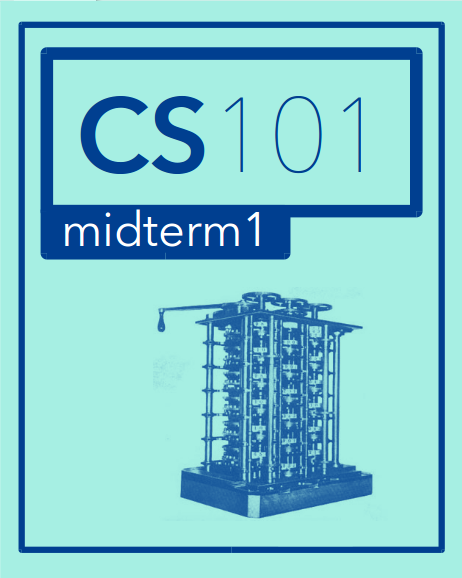
\includegraphics[width=2in]{../img/midterm1-header.png}
\end{center}

\bigskip
\noindent
\begin{itemize}
\item \textbf{Be sure to enter your \underline{NetID} and \underline{the code below} on your Scantron}.
\item Do not turn this page until instructed to do so.
\item There are 30 questions, worth 1 point each.
\item Each question has only \textbf{one} correct answer.
\item You must not communicate with other students during this test.
\item No books, notes, or electronic devices are permitted.
\item This is a 60-minute exam.
\item There are several different versions of this exam.
\end{itemize}

\bigskip\bigskip
\noindent
\textbf{\Large 1. Fill in your information:}

\bigskip
{\Large\bf
\begin{tabular}{ll}
Full Name: & \underbar{\hskip 8cm} \\[0.5em]
UIN (Student Number): & \underbar{\hskip 8cm} \\[0.5em]
NetID: & \underbar{\hskip 8cm}
\end{tabular}
}

\bigskip
\bigskip
\noindent
\textbf{\Large 2. Fill in the following answers on the Scantron form:}

%%%%%%%%%%%%%%%%%%%%%%%%%%%%%%%%%%%%%%%%%%%%%%%%%%%%%%%%%
%%%%%%%%%%%%%%%%%%%%%%%%%%%%%%%%%%%%%%%%%%%%%%%%%%%%%%%%%

\begin{enumerate}
\item[92.] B
\item[93.] D
\item[94.] B
\item[95.] D
\item[96.] C
\end{enumerate}

\newpage

% Zone 1


%%%%%%%%%%%%%%%%%%%%%%%%%%%%%%%%%%%%%%%%%%%%%%%%%%%%%%%%%



\newpage
\noindent
1. (1 point)
Consider the following program:
\begin{verbatim}
s="ECTOR"
t="GAWAIN"
x=(len(s)/(len(t)-1))+1
\end{verbatim}
What is the \textbf{type} of \texttt{x} after this program is executed?


\begin{enumerate}
\item[(A)] $\bigstar$ 
\begin{verbatim}Float\end{verbatim}

\item[(B)]
\begin{verbatim}Boolean\end{verbatim}

\item[(C)]
\begin{verbatim}Integer\end{verbatim}

\item[(D)]
\begin{verbatim}String\end{verbatim}

\item[(E)]
\begin{verbatim}None\end{verbatim}

\end{enumerate}

\vspace*{2em}
\hrule
\vspace{2em}

\noindent {\bf Solution.} 
\vspace{2em}
\hrule height 2pt


\newpage
\noindent
2. (1 point)
Consider the following program:
\begin{verbatim}
x=0
for i in range(2,7):
    if i%3==0:
        x+=3
    elif i%2==0:
        x+=2
    else:
        x+=1
\end{verbatim}
What is the \textbf{value} of \texttt{x} after this program is executed?


\begin{enumerate}
\item[(A)]
\begin{verbatim}14\end{verbatim}

\item[(B)]
\begin{verbatim}10\end{verbatim}

\item[(C)] $\bigstar$ 
\begin{verbatim}11\end{verbatim}

\item[(D)]
\begin{verbatim}13\end{verbatim}

\item[(E)]
\begin{verbatim}12\end{verbatim}

\end{enumerate}

\vspace*{2em}
\hrule
\vspace{2em}

\noindent {\bf Solution.} 
\vspace{2em}
\hrule height 2pt


\newpage
\noindent
3. (1 point)
Consider the following program:
\begin{verbatim}
a=["merlin","sir agravaine","king pellinore"]
b=[ ]
for i in range(0,3):
    b.append(a[0-i].title())
\end{verbatim}
What is the \textbf{value} of b after this program is executed?


\begin{enumerate}
\item[(A)] $\bigstar$ 
\begin{verbatim}['Merlin', 'King Pellinore', 'Sir Agravaine']\end{verbatim}

\item[(B)]
\begin{verbatim}['King Pellinore', 'Sir Agravaine', 'Merlin']\end{verbatim}

\item[(C)]
\begin{verbatim}['Sir Agravaine', 'King Pellinore']\end{verbatim}

\item[(D)]
\begin{verbatim}[ ]\end{verbatim}

\item[(E)]
\begin{verbatim}['King Pellinore', 'Sir Agravaine']\end{verbatim}

\end{enumerate}

\vspace*{2em}
\hrule
\vspace{2em}

\noindent {\bf Solution.} 
\vspace{2em}
\hrule height 2pt


\newpage
\noindent
4. (1 point)
For this problem, you should compose a function which accomplishes a given task using the available code blocks arranged in the correct functional order.  \emph{We ignore indentation for this problem.}

\texttt{find\_max} should accept a \texttt{list} and return the value of the maximum item in the \texttt{list}.  (\texttt{None} is always the lowest value in any numeric comparison, so you may use it as an initializer.)

\begin{verbatim}
def find_max(my_list):
\end{verbatim}

\begin{enumerate}[1]
\item \texttt{max\_val = i}
\item \texttt{max\_val = None}
\item \texttt{for i in range(len(my\_list)):}
\item \texttt{if i > max\_val:}
\item \texttt{max\_val = my\_list[i]}
\item \texttt{return max\_val}
\item \texttt{for i in range(my\_list):}
\item \texttt{if my\_list[i] > max\_val:}
\item \texttt{print(max\_val)}
\end{enumerate}



\begin{enumerate}
\item[(A)]
2, 3, 8, 1, 6

\item[(B)]
2, 3, 4, 1, 6

\item[(C)] $\bigstar$ 
2, 3, 8, 5, 6

\item[(D)]
2, 7, 4, 5, 6

\item[(E)]
3, 2, 8, 5, 9

\end{enumerate}

\vspace*{2em}
\hrule
\vspace{2em}

\noindent {\bf Solution.} 
\vspace{2em}
\hrule height 2pt


\newpage
\noindent
5. (1 point)
Consider the following program:
\begin{verbatim}
i=2
x=3
while i < 7:
    x+=i
    i+=2
\end{verbatim}
What is the \textbf{value} of \texttt{x} after this program is executed?


\begin{enumerate}
\item[(A)]
\begin{verbatim}13\end{verbatim}

\item[(B)]
\begin{verbatim}12\end{verbatim}

\item[(C)]
\begin{verbatim}14\end{verbatim}

\item[(D)] $\bigstar$ 
\begin{verbatim}15\end{verbatim}

\item[(E)]
\begin{verbatim}11\end{verbatim}

\end{enumerate}

\vspace*{2em}
\hrule
\vspace{2em}

\noindent {\bf Solution.} 
\vspace{2em}
\hrule height 2pt


\newpage
\noindent
6. (1 point)
Consider the following program:
\begin{verbatim}
x=str("1"*3)
\end{verbatim}
What is the \textbf{value} of \texttt{x} after this program is executed?


\begin{enumerate}
\item[(A)]
None of the other answers are correct.

\item[(B)]
\begin{verbatim}"3"\end{verbatim}

\item[(C)]
\begin{verbatim}111\end{verbatim}

\item[(D)]
\begin{verbatim}3\end{verbatim}

\item[(E)] $\bigstar$ 
\begin{verbatim}"111"\end{verbatim}

\end{enumerate}

\vspace*{2em}
\hrule
\vspace{2em}

\noindent {\bf Solution.} 
\vspace{2em}
\hrule height 2pt


\newpage
\noindent
7. (1 point)
What is the result of the following expression?
\begin{verbatim}
[ 1, 2, 3 ] * 3.0
\end{verbatim}


\begin{enumerate}
\item[(A)]
\begin{verbatim}None of the above.\end{verbatim}

\item[(B)] $\bigstar$ 
\begin{verbatim}[1, 2, 3, 1, 2, 3, 1, 2, 3]\end{verbatim}

\item[(C)]
\begin{verbatim}[3.0, 6.0, 9.0]\end{verbatim}

\item[(D)]
\begin{verbatim}[1.0, 2.0, 3.0, 1.0, 2.0, 3.0, 1.0, 2.0, 3.0]\end{verbatim}

\item[(E)]
\begin{verbatim}[3, 6, 9]\end{verbatim}

\end{enumerate}

\vspace*{2em}
\hrule
\vspace{2em}

\noindent {\bf Solution.} 
\vspace{2em}
\hrule height 2pt


\newpage
\noindent
8. (1 point)
Consider the following program:
\begin{verbatim}
x=[1,2,3]
def f(a):
    s=""
    a.reverse()
    for i in a:
        s+=str(i)
    return s

x.append(f(x))
\end{verbatim}
What is the \textbf{value} of \texttt{x} after this program is executed?


\begin{enumerate}
\item[(A)]
\begin{verbatim}[1, 2, 3, 6]\end{verbatim}

\item[(B)]
\begin{verbatim}[1, 2, 3]\end{verbatim}

\item[(C)]
\begin{verbatim}[3, 2, 1]\end{verbatim}

\item[(D)] $\bigstar$ 
\begin{verbatim}[3, 2, 1, '321']\end{verbatim}

\item[(E)]
\begin{verbatim}[1, 2, 3, '321']\end{verbatim}

\end{enumerate}

\vspace*{2em}
\hrule
\vspace{2em}

\noindent {\bf Solution.} 
\vspace{2em}
\hrule height 2pt


\newpage
\noindent
9. (1 point)
Consider the following program.
\begin{verbatim}
s="ABCBA"
x=0
y=len(s)-1
while s[x]==s[y] and x<y:
    x+=1
    y-=1
\end{verbatim}
After it is run, what is the final \textbf{value} of \texttt{x}?


\begin{enumerate}
\item[(A)]
\begin{verbatim}0\end{verbatim}

\item[(B)]
\begin{verbatim}3\end{verbatim}

\item[(C)]
\begin{verbatim}1\end{verbatim}

\item[(D)]
\begin{verbatim}4\end{verbatim}

\item[(E)] $\bigstar$ 
\begin{verbatim}2\end{verbatim}

\end{enumerate}

\vspace*{2em}
\hrule
\vspace{2em}

\noindent {\bf Solution.} 
\vspace{2em}
\hrule height 2pt


\newpage
\noindent
10. (1 point)
Consider the following program:
\begin{verbatim}
s="TRIS %i"
t="ISEU"
x=len(s) % len(t[2:-1])
\end{verbatim}
What is the \textbf{type} of \texttt{x} after this program is executed?


\begin{enumerate}
\item[(A)]
\begin{verbatim}Float\end{verbatim}

\item[(B)]
\begin{verbatim}None\end{verbatim}

\item[(C)]
\begin{verbatim}String\end{verbatim}

\item[(D)]
\begin{verbatim}Boolean\end{verbatim}

\item[(E)] $\bigstar$ 
\begin{verbatim}Integer\end{verbatim}

\end{enumerate}

\vspace*{2em}
\hrule
\vspace{2em}

\noindent {\bf Solution.} 
\vspace{2em}
\hrule height 2pt


\newpage
\noindent
11. (1 point)
Consider the following program:
\begin{verbatim}
x=[1,2,3,4,5,6,7,8,9]
x=x[2:-2]
i=1
while i <= 3:
    x[i]+=1
    i+=1
\end{verbatim}
What is the \textbf{value} of \texttt{x} after this program is executed?


\begin{enumerate}
\item[(A)]
\begin{verbatim}[3, 5, 6, 7, 7, 8]\end{verbatim}

\item[(B)]
\begin{verbatim}[2, 4, 5, 5, 7, 7]\end{verbatim}

\item[(C)] $\bigstar$ 
\begin{verbatim}[3, 5, 6, 7, 7]\end{verbatim}

\item[(D)]
\begin{verbatim}[3, 5, 7, 7]\end{verbatim}

\item[(E)]
\begin{verbatim}[2, 4, 5, 6, 7, 7]\end{verbatim}

\end{enumerate}

\vspace*{2em}
\hrule
\vspace{2em}

\noindent {\bf Solution.} 
\vspace{2em}
\hrule height 2pt


\newpage
\noindent
12. (1 point)
Consider the following program:
\begin{verbatim}
a=["A","C","C","I","O"]
a.sort()
a[0]=a[-1]
x=""
for e in a:
    x=x+e
\end{verbatim}
What is the \textbf{value} of \texttt{x} after this program is executed?


\begin{enumerate}
\item[(A)]
\begin{verbatim}"ICCOI"\end{verbatim}

\item[(B)]
None of the other answers are correct.

\item[(C)]
\begin{verbatim}"ACCIA"\end{verbatim}

\item[(D)]
\begin{verbatim}"ACCOA"\end{verbatim}

\item[(E)] $\bigstar$ 
\begin{verbatim}"OCCIO"\end{verbatim}

\end{enumerate}

\vspace*{2em}
\hrule
\vspace{2em}

\noindent {\bf Solution.} 
\vspace{2em}
\hrule height 2pt


\newpage
\noindent
13. (1 point)
Consider the following incomplete program.
\begin{verbatim}
sum=0
for i in range(0,100):
    ???

\end{verbatim}
The program is intended to sum all of the integers between 1 and 100 (inclusive). What should replace the three question marks to complete the program?


\begin{enumerate}
\item[(A)]
\begin{verbatim}sum=sum+i \end{verbatim}

\item[(B)] $\bigstar$ 
\begin{verbatim}sum=sum+i+1 \end{verbatim}

\item[(C)]
\begin{verbatim}sum+1=sum \end{verbatim}

\item[(D)]
\begin{verbatim}sum=sum+1\end{verbatim}

\end{enumerate}

\vspace*{2em}
\hrule
\vspace{2em}

\noindent {\bf Solution.} 
\vspace{2em}
\hrule height 2pt


\newpage
\noindent
14. (1 point)
Consider the following program.
\begin{verbatim}
x=1
i=0
while(x*x)<=9:
    i=i+(x*x)
    x=x+1
\end{verbatim}
After it is run, what is the final \textbf{value} of \texttt{x}?


\begin{enumerate}
\item[(A)]
\begin{verbatim}3\end{verbatim}

\item[(B)]
\begin{verbatim}14\end{verbatim}

\item[(C)] $\bigstar$ 
\begin{verbatim}4\end{verbatim}

\item[(D)]
\begin{verbatim}30\end{verbatim}

\item[(E)]
\begin{verbatim}5\end{verbatim}

\end{enumerate}

\vspace*{2em}
\hrule
\vspace{2em}

\noindent {\bf Solution.} 
\vspace{2em}
\hrule height 2pt


\newpage
\noindent
15. (1 point)
Consider the following program:
\begin{verbatim}
pi="3.14159"
e="2.71828"
x=pi in pi*len(e)
\end{verbatim}
What is the \textbf{type} of \texttt{x} after this program is executed?


\begin{enumerate}
\item[(A)]
\begin{verbatim}Integer\end{verbatim}

\item[(B)]
\begin{verbatim}String\end{verbatim}

\item[(C)]
\begin{verbatim}None\end{verbatim}

\item[(D)] $\bigstar$ 
\begin{verbatim}Boolean\end{verbatim}

\item[(E)]
\begin{verbatim}Float\end{verbatim}

\end{enumerate}

\vspace*{2em}
\hrule
\vspace{2em}

\noindent {\bf Solution.} 
\vspace{2em}
\hrule height 2pt


\newpage
\noindent
16. (1 point)
Consider the following incomplete function.
\begin{verbatim}
def isdivisible(m,n):
    if ???:
        return False
    else:
        return True
\end{verbatim}
The function is intended to return True if the input parameter m is evenly divisible by the parameter n and False otherwise. For example, \verb|isdivisible(4,2)| should return \verb|True|, but \verb|isdivisible(5,3)| should return \verb|False|. What should replace the three question marks to complete the function?


\begin{enumerate}
\item[(A)] $\bigstar$ 
\begin{verbatim}(m % n) != 0 \end{verbatim}

\item[(B)]
\begin{verbatim}(n // m) == 0 \end{verbatim}

\item[(C)]
\begin{verbatim}(n % m) == 0 \end{verbatim}

\item[(D)]
\begin{verbatim}(m // n) != 0 \end{verbatim}

\end{enumerate}

\vspace*{2em}
\hrule
\vspace{2em}

\noindent {\bf Solution.} 
\vspace{2em}
\hrule height 2pt


\newpage
\noindent
17. (1 point)
Consider the following incomplete Python program.
\begin{verbatim}
s="".join(["1","0","2","1"])
x=0
for i in range(len(s)-1):
    x+=int(???)
\end{verbatim}
What should replace the three question marks so the resulting value of \texttt{x} is 33?


\begin{enumerate}
\item[(A)]
\begin{verbatim}s[i:i-1]\end{verbatim}

\item[(B)]
\begin{verbatim}s[i:i+1]\end{verbatim}

\item[(C)] $\bigstar$ 
\begin{verbatim}s[i:i+2]\end{verbatim}

\item[(D)]
\begin{verbatim}s[i+1:i+2]\end{verbatim}

\end{enumerate}

\vspace*{2em}
\hrule
\vspace{2em}

\noindent {\bf Solution.} 
\vspace{2em}
\hrule height 2pt


\newpage
\noindent
18. (1 point)
Consider the following program:
\begin{verbatim}
s="Hobbes"
i=0
x=-1
while i<len(s):
    if s[i]=='b':
        x=i
    i+=1
\end{verbatim}
What is the \textbf{value} of \texttt{x} after this program is executed?


\begin{enumerate}
\item[(A)] $\bigstar$ 
\begin{verbatim}3\end{verbatim}

\item[(B)]
\begin{verbatim}-1\end{verbatim}

\item[(C)]
\begin{verbatim}2\end{verbatim}

\item[(D)]
\begin{verbatim}4\end{verbatim}

\item[(E)]
\begin{verbatim}5\end{verbatim}

\end{enumerate}

\vspace*{2em}
\hrule
\vspace{2em}

\noindent {\bf Solution.} 
\vspace{2em}
\hrule height 2pt


\newpage
\noindent
19. (1 point)
Evaluate the following expression:
\begin{verbatim}
len("ABCDE"[1:4])
\end{verbatim}
What value is produced?


\begin{enumerate}
\item[(A)]
1

\item[(B)]
4

\item[(C)]
5

\item[(D)] $\bigstar$ 
3

\end{enumerate}

\vspace*{2em}
\hrule
\vspace{2em}

\noindent {\bf Solution.} 
\vspace{2em}
\hrule height 2pt


\newpage
\noindent
20. (1 point)
Evaluate the following expression:
\begin{verbatim}
[1,2]+[len("3")]
\end{verbatim}
What value is produced?


\begin{enumerate}
\item[(A)]
\begin{verbatim}[1,2,1,2,1,2]\end{verbatim}

\item[(B)]
\begin{verbatim}[1,2,"3"]\end{verbatim}

\item[(C)]
\begin{verbatim}[1,2,3]\end{verbatim}

\item[(D)] $\bigstar$ 
\begin{verbatim}[1,2,1]\end{verbatim}

\end{enumerate}

\vspace*{2em}
\hrule
\vspace{2em}

\noindent {\bf Solution.} 
\vspace{2em}
\hrule height 2pt


\newpage
\noindent
21. (1 point)
How can the following mathematical equation be implemented as a Python expression? Assume \verb|a|, \verb|b|, and \verb|sin| have already been defined.
$$a \sin(a^b - b)$$


\begin{enumerate}
\item[(A)] $\bigstar$ 
\begin{verbatim}a*sin(a**b - b)\end{verbatim}

\item[(B)]
\begin{verbatim}a sin(a**b - b)\end{verbatim}

\item[(C)]
\begin{verbatim}a*sin(b^a - b)\end{verbatim}

\item[(D)]
\begin{verbatim}a*sin(a^b - b)\end{verbatim}

\item[(E)]
None of the other answers are correct.

\end{enumerate}

\vspace*{2em}
\hrule
\vspace{2em}

\noindent {\bf Solution.} 
\vspace{2em}
\hrule height 2pt


\newpage
\noindent
22. (1 point)
Consider the following program:
\begin{verbatim}
def fix(s):
    a=list(s)
    a.sort()
    return ''.join(a)

x=["one","two","eleven","twelve"]
s1=fix(x[0]+x[-1])
s2=fix(x[1]+x[-2])

if s1<s2:
    x.sort()
elif s1>s2:
    x.reverse()
else:
    x.append("six")
\end{verbatim}
What is the \textbf{value} of \texttt{x} after this program is executed?


\begin{enumerate}
\item[(A)]
\begin{verbatim}['eleven', 'one', 'twelve', 'two']\end{verbatim}

\item[(B)]
\begin{verbatim}['one', 'two', 'eleven', 'twelve']\end{verbatim}

\item[(C)] $\bigstar$ 
\begin{verbatim}['one', 'two', 'eleven', 'twelve', 'six']\end{verbatim}

\item[(D)]
\begin{verbatim}['two', 'twelve', 'one', 'eleven', 'six']\end{verbatim}

\item[(E)]
\begin{verbatim}['twelve', 'eleven', 'two', 'one']\end{verbatim}

\end{enumerate}

\vspace*{2em}
\hrule
\vspace{2em}

\noindent {\bf Solution.} 
\vspace{2em}
\hrule height 2pt


\newpage
\noindent
23. (1 point)
Consider the following program.
\begin{verbatim}
kay = 2
wart = 3

def knight(kay,wart):
    wart += 2
    kay += 3
    return wart + kay

kay = knight(wart, kay) + knight(kay, wart)
\end{verbatim}
After it is run, what is the final \textbf{value} of \texttt{kay}?


\begin{enumerate}
\item[(A)]
\begin{verbatim}5\end{verbatim}

\item[(B)]
\begin{verbatim}2\end{verbatim}

\item[(C)] $\bigstar$ 
None of the other answers are correct.

\item[(D)]
\begin{verbatim}3\end{verbatim}

\end{enumerate}

\vspace*{2em}
\hrule
\vspace{2em}

\noindent {\bf Solution.} 
\vspace{2em}
\hrule height 2pt


\newpage
\noindent
24. (1 point)
Consider the following program.
\begin{verbatim}
def artificing(s):
    return s+"%i" % 2
    return s*2
    return s

s=artificing("MERLIN")
\end{verbatim}
After it is run, what is the final \textbf{value} of s?


\begin{enumerate}
\item[(A)] $\bigstar$ 
\begin{verbatim}"MERLIN2"\end{verbatim}

\item[(B)]
\begin{verbatim}"MERLIN%i"\end{verbatim}

\item[(C)]
\begin{verbatim}"MERLINMERLIN"\end{verbatim}

\item[(D)]
\begin{verbatim}0\end{verbatim}

\item[(E)]
\begin{verbatim}None\end{verbatim}

\end{enumerate}

\vspace*{2em}
\hrule
\vspace{2em}

\noindent {\bf Solution.} 
\vspace{2em}
\hrule height 2pt


\newpage
\noindent
25. (1 point)
Consider the following program:
\begin{verbatim}
x=3
a=7
if (a%3)==2:
    x=x**2
elif(a%3)==1:
    x=x**1
else:
    x=x**0
\end{verbatim}
What is the \textbf{value} of \texttt{x} after this program is executed?


\begin{enumerate}
\item[(A)]
None of the other answers are correct.

\item[(B)]
\begin{verbatim}7\end{verbatim}

\item[(C)] $\bigstar$ 
\begin{verbatim}3\end{verbatim}

\item[(D)]
\begin{verbatim}1\end{verbatim}

\item[(E)]
\begin{verbatim}9\end{verbatim}

\end{enumerate}

\vspace*{2em}
\hrule
\vspace{2em}

\noindent {\bf Solution.} 
\vspace{2em}
\hrule height 2pt


\newpage
\noindent
26. (1 point)
Consider the following program:
\begin{verbatim}
x="KING ARTHUR-MORGANA LEFAY-SIR BEDIVERE".split("-")
y=x
x=y.reverse()
\end{verbatim}
What is the \textbf{value} of \texttt{x} after this program is executed?


\begin{enumerate}
\item[(A)]
\begin{verbatim}['SIR BEDIVERE', 'MORGANA LEFAY', 'KING ARTHUR']\end{verbatim}

\item[(B)]
\begin{verbatim}['KING', 'ARTHUR-MORGANA', 'LEFAY-SIR', 'BEDIVERE']\end{verbatim}

\item[(C)]
\begin{verbatim}['KING ARTHUR', 'MORGANA LEFAY', 'SIR BEDIVERE']\end{verbatim}

\item[(D)] $\bigstar$ 
\begin{verbatim}None\end{verbatim}

\item[(E)]
\begin{verbatim}['BEDIVERE', 'LEFAY-SIR', 'ARTHUR-MORGANA', 'KING']\end{verbatim}

\end{enumerate}

\vspace*{2em}
\hrule
\vspace{2em}

\noindent {\bf Solution.} 
\vspace{2em}
\hrule height 2pt


\newpage
\noindent
27. (1 point)
Consider the following program:
\begin{verbatim}
a=3
b=4
if a!=b:
    a=b
elif a==4:
    a=5
else:
    b=a
\end{verbatim}
What is the \textbf{value} of a after this program is executed?


\begin{enumerate}
\item[(A)]
None of the other answers are correct.

\item[(B)]
\begin{verbatim}3\end{verbatim}

\item[(C)] $\bigstar$ 
\begin{verbatim}4\end{verbatim}

\item[(D)]
\begin{verbatim}5\end{verbatim}

\item[(E)]
\begin{verbatim}7\end{verbatim}

\end{enumerate}

\vspace*{2em}
\hrule
\vspace{2em}

\noindent {\bf Solution.} 
\vspace{2em}
\hrule height 2pt


\newpage
\noindent
28. (1 point)
Consider the following program.
\begin{verbatim}
x=[]
for j in range(0,5):
    if (j%2)==0:
        x.append("-")
    if (j%5)==0:
        x.append("*")
\end{verbatim}
After it is run, what is the final \textbf{value} of \texttt{x}?


\begin{enumerate}
\item[(A)]
\begin{verbatim}["*","-","*","*"]\end{verbatim}

\item[(B)] $\bigstar$ 
\begin{verbatim}["-","*","-","-"]\end{verbatim}

\item[(C)]
\begin{verbatim}["-","-","*"]\end{verbatim}

\item[(D)]
None of the other answers are correct.

\item[(E)]
\begin{verbatim}["-","*","-"]\end{verbatim}

\end{enumerate}

\vspace*{2em}
\hrule
\vspace{2em}

\noindent {\bf Solution.} 
\vspace{2em}
\hrule height 2pt


\newpage
\noindent
29. (1 point)
Consider the following program:
\begin{verbatim}
s="G+R+A+I+L"
x=s.split("+")[1:-2]
\end{verbatim}
What is the \textbf{value} of \texttt{x} after this program is executed?


\begin{enumerate}
\item[(A)]
\begin{verbatim}'RAI'\end{verbatim}

\item[(B)] $\bigstar$ 
\begin{verbatim}['R','A']\end{verbatim}

\item[(C)]
\begin{verbatim}None\end{verbatim}

\item[(D)]
\begin{verbatim}3\end{verbatim}

\item[(E)]
\begin{verbatim}False\end{verbatim}

\end{enumerate}

\vspace*{2em}
\hrule
\vspace{2em}

\noindent {\bf Solution.} 
\vspace{2em}
\hrule height 2pt


\newpage
\noindent
30. (1 point)
Consider the following Python program.
\begin{verbatim}
e=[1,3,5,7,9,11]
d=[0,0,0]
for i in range(0,len(e)):
    d[i%3]+=e[i]
x=d[1]
\end{verbatim}
After it is run, what is the final \textbf{value} of \texttt{x}?


\begin{enumerate}
\item[(A)]
\begin{verbatim}0\end{verbatim}

\item[(B)]
\begin{verbatim}16\end{verbatim}

\item[(C)]
\begin{verbatim}3\end{verbatim}

\item[(D)]
\begin{verbatim}8\end{verbatim}

\item[(E)] $\bigstar$ 
\begin{verbatim}12\end{verbatim}

\end{enumerate}

\vspace*{2em}
\hrule
\vspace{2em}

\noindent {\bf Solution.} 
\vspace{2em}
\hrule height 2pt

%%%%%%%%%%%%%%%%%%%%%%%%%%%%%%%%%%%%%%%%%%%%%%%%%%%%%%%%%%%%%%%%%%%%%%
%%%%%%%%%%%%%%%%%%%%%%%%%%%%%%%%%%%%%%%%%%%%%%%%%%%%%%%%%%%%%%%%%%%%%%
%%%%%%%%%%%%%%%%%%%%%%%%%%%%%%%%%%%%%%%%%%%%%%%%%%%%%%%%%%%%%%%%%%%%%%
%%%%%%%%%%%%%%%%%%%%%%%%%%%%%%%%%%%%%%%%%%%%%%%%%%%%%%%%%%%%%%%%%%%%%%
% Exam number 43

\message{Exam 43/50}
\cleardoublepage
\setcounter{page}{1}


\begin{center}
%\textbf{\Large CS 101 Midterm \#1}
%
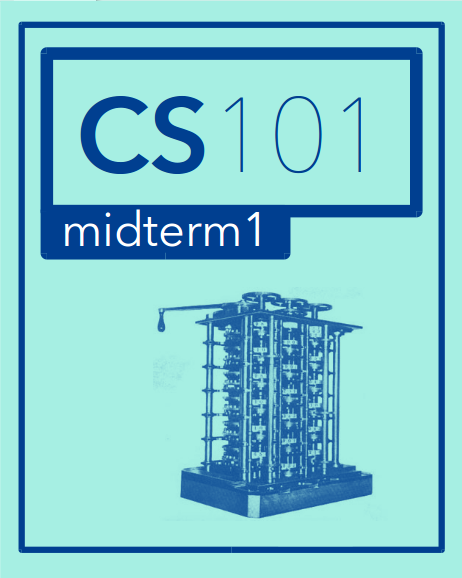
\includegraphics[width=2in]{../img/midterm1-header.png}
\end{center}

\bigskip
\noindent
\begin{itemize}
\item \textbf{Be sure to enter your \underline{NetID} and \underline{the code below} on your Scantron}.
\item Do not turn this page until instructed to do so.
\item There are 30 questions, worth 1 point each.
\item Each question has only \textbf{one} correct answer.
\item You must not communicate with other students during this test.
\item No books, notes, or electronic devices are permitted.
\item This is a 60-minute exam.
\item There are several different versions of this exam.
\end{itemize}

\bigskip\bigskip
\noindent
\textbf{\Large 1. Fill in your information:}

\bigskip
{\Large\bf
\begin{tabular}{ll}
Full Name: & \underbar{\hskip 8cm} \\[0.5em]
UIN (Student Number): & \underbar{\hskip 8cm} \\[0.5em]
NetID: & \underbar{\hskip 8cm}
\end{tabular}
}

\bigskip
\bigskip
\noindent
\textbf{\Large 2. Fill in the following answers on the Scantron form:}

%%%%%%%%%%%%%%%%%%%%%%%%%%%%%%%%%%%%%%%%%%%%%%%%%%%%%%%%%
%%%%%%%%%%%%%%%%%%%%%%%%%%%%%%%%%%%%%%%%%%%%%%%%%%%%%%%%%

\begin{enumerate}
\item[92.] C
\item[93.] D
\item[94.] B
\item[95.] E
\item[96.] D
\end{enumerate}

\newpage

% Zone 1


%%%%%%%%%%%%%%%%%%%%%%%%%%%%%%%%%%%%%%%%%%%%%%%%%%%%%%%%%



\newpage
\noindent
1. (1 point)
Evaluate the following expression:
\begin{verbatim}
len("ABCDE"[1:4])
\end{verbatim}
What value is produced?


\begin{enumerate}
\item[(A)]
5

\item[(B)] $\bigstar$ 
3

\item[(C)]
1

\item[(D)]
4

\end{enumerate}

\vspace*{2em}
\hrule
\vspace{2em}

\noindent {\bf Solution.} 
\vspace{2em}
\hrule height 2pt


\newpage
\noindent
2. (1 point)
Consider the following program:
\begin{verbatim}
a=3
b=4
if a==3:
    b=a
elif a==4:
    a=5
else:
    a=b
\end{verbatim}
What is the \textbf{value} of a after this program is executed?


\begin{enumerate}
\item[(A)] $\bigstar$ 
\begin{verbatim}3\end{verbatim}

\item[(B)]
None of the other answers are correct.

\item[(C)]
\begin{verbatim}7\end{verbatim}

\item[(D)]
\begin{verbatim}4\end{verbatim}

\item[(E)]
\begin{verbatim}5\end{verbatim}

\end{enumerate}

\vspace*{2em}
\hrule
\vspace{2em}

\noindent {\bf Solution.} 
\vspace{2em}
\hrule height 2pt


\newpage
\noindent
3. (1 point)
Consider the following program:
\begin{verbatim}
x=str("1"*3)
\end{verbatim}
What is the \textbf{value} of \texttt{x} after this program is executed?


\begin{enumerate}
\item[(A)]
\begin{verbatim}3\end{verbatim}

\item[(B)]
\begin{verbatim}"3"\end{verbatim}

\item[(C)]
None of the other answers are correct.

\item[(D)]
\begin{verbatim}111\end{verbatim}

\item[(E)] $\bigstar$ 
\begin{verbatim}"111"\end{verbatim}

\end{enumerate}

\vspace*{2em}
\hrule
\vspace{2em}

\noindent {\bf Solution.} 
\vspace{2em}
\hrule height 2pt


\newpage
\noindent
4. (1 point)
Consider the following program:
\begin{verbatim}
x=0
for i in range(2,7):
    if i%3==0:
        x+=3
    elif i%2==0:
        x+=2
    else:
        x+=1
\end{verbatim}
What is the \textbf{value} of \texttt{x} after this program is executed?


\begin{enumerate}
\item[(A)]
\begin{verbatim}10\end{verbatim}

\item[(B)] $\bigstar$ 
\begin{verbatim}11\end{verbatim}

\item[(C)]
\begin{verbatim}13\end{verbatim}

\item[(D)]
\begin{verbatim}14\end{verbatim}

\item[(E)]
\begin{verbatim}12\end{verbatim}

\end{enumerate}

\vspace*{2em}
\hrule
\vspace{2em}

\noindent {\bf Solution.} 
\vspace{2em}
\hrule height 2pt


\newpage
\noindent
5. (1 point)
Consider the following program.
\begin{verbatim}
s="BBCAA"
x=0
y=len(s)-1
while s[x]!=s[y] and x<len(s):
    x+=1
    y-=1
\end{verbatim}
After it is run, what is the final \textbf{value} of \texttt{x}?


\begin{enumerate}
\item[(A)]
\begin{verbatim}0\end{verbatim}

\item[(B)]
\begin{verbatim}1\end{verbatim}

\item[(C)]
\begin{verbatim}4\end{verbatim}

\item[(D)]
\begin{verbatim}3\end{verbatim}

\item[(E)] $\bigstar$ 
\begin{verbatim}2\end{verbatim}

\end{enumerate}

\vspace*{2em}
\hrule
\vspace{2em}

\noindent {\bf Solution.} 
\vspace{2em}
\hrule height 2pt


\newpage
\noindent
6. (1 point)
Consider the following program.
\begin{verbatim}
kay = 2
wart = 3

def knight(kay,wart):
    wart += 2
    kay += 3
    return wart + kay

wart = knight(kay, kay) + knight(wart, wart)
\end{verbatim}
After it is run, what is the final \textbf{value} of \texttt{wart}?


\begin{enumerate}
\item[(A)]
\begin{verbatim}5\end{verbatim}

\item[(B)]
\begin{verbatim}3\end{verbatim}

\item[(C)]
\begin{verbatim}2\end{verbatim}

\item[(D)] $\bigstar$ 
None of the other answers are correct.

\end{enumerate}

\vspace*{2em}
\hrule
\vspace{2em}

\noindent {\bf Solution.} 
\vspace{2em}
\hrule height 2pt


\newpage
\noindent
7. (1 point)
Consider the following program:
\begin{verbatim}
def fix(s):
    a=list(s)
    a.sort()
    return ''.join(a)

x=["one","two","eleven","twelve"]
s1=fix(x[0]+x[-1])
s2=fix(x[1]+x[-2])

if s1<s2:
    x.sort()
elif s1>s2:
    x.reverse()
else:
    x.append("six")
\end{verbatim}
What is the \textbf{value} of \texttt{x} after this program is executed?


\begin{enumerate}
\item[(A)]
\begin{verbatim}['twelve', 'eleven', 'two', 'one']\end{verbatim}

\item[(B)]
\begin{verbatim}['one', 'two', 'eleven', 'twelve']\end{verbatim}

\item[(C)] $\bigstar$ 
\begin{verbatim}['one', 'two', 'eleven', 'twelve', 'six']\end{verbatim}

\item[(D)]
\begin{verbatim}['two', 'twelve', 'one', 'eleven', 'six']\end{verbatim}

\item[(E)]
\begin{verbatim}['eleven', 'one', 'twelve', 'two']\end{verbatim}

\end{enumerate}

\vspace*{2em}
\hrule
\vspace{2em}

\noindent {\bf Solution.} 
\vspace{2em}
\hrule height 2pt


\newpage
\noindent
8. (1 point)
Consider the following program:
\begin{verbatim}
s="ECTOR"
t="GAWAIN"
x=(len(s)/(len(t)-1))+1
\end{verbatim}
What is the \textbf{type} of \texttt{x} after this program is executed?


\begin{enumerate}
\item[(A)]
\begin{verbatim}None\end{verbatim}

\item[(B)]
\begin{verbatim}String\end{verbatim}

\item[(C)]
\begin{verbatim}Boolean\end{verbatim}

\item[(D)] $\bigstar$ 
\begin{verbatim}Float\end{verbatim}

\item[(E)]
\begin{verbatim}Integer\end{verbatim}

\end{enumerate}

\vspace*{2em}
\hrule
\vspace{2em}

\noindent {\bf Solution.} 
\vspace{2em}
\hrule height 2pt


\newpage
\noindent
9. (1 point)
Consider the following program:
\begin{verbatim}
i=3
x=2
while i < 7:
    x+=i
    i+=2
\end{verbatim}
What is the \textbf{value} of \texttt{x} after this program is executed?


\begin{enumerate}
\item[(A)] $\bigstar$ 
\begin{verbatim}10\end{verbatim}

\item[(B)]
\begin{verbatim}12\end{verbatim}

\item[(C)]
\begin{verbatim}14\end{verbatim}

\item[(D)]
\begin{verbatim}11\end{verbatim}

\item[(E)]
\begin{verbatim}13\end{verbatim}

\end{enumerate}

\vspace*{2em}
\hrule
\vspace{2em}

\noindent {\bf Solution.} 
\vspace{2em}
\hrule height 2pt


\newpage
\noindent
10. (1 point)
Consider the following program:
\begin{verbatim}
s="G+R+A+I+L"
x=s.split("+")[1:-2]
\end{verbatim}
What is the \textbf{value} of \texttt{x} after this program is executed?


\begin{enumerate}
\item[(A)] $\bigstar$ 
\begin{verbatim}['R','A']\end{verbatim}

\item[(B)]
\begin{verbatim}False\end{verbatim}

\item[(C)]
\begin{verbatim}None\end{verbatim}

\item[(D)]
\begin{verbatim}3\end{verbatim}

\item[(E)]
\begin{verbatim}'RAI'\end{verbatim}

\end{enumerate}

\vspace*{2em}
\hrule
\vspace{2em}

\noindent {\bf Solution.} 
\vspace{2em}
\hrule height 2pt


\newpage
\noindent
11. (1 point)
How can the following mathematical equation be implemented as a Python expression? Assume \verb|a|, \verb|b|, and \verb|sin| have already been defined.
$$a \sin(a^b - b)$$


\begin{enumerate}
\item[(A)] $\bigstar$ 
\begin{verbatim}a*sin(a**b - b)\end{verbatim}

\item[(B)]
\begin{verbatim}a*sin(a^b - b)\end{verbatim}

\item[(C)]
None of the other answers are correct.

\item[(D)]
\begin{verbatim}a sin(a**b - b)\end{verbatim}

\item[(E)]
\begin{verbatim}a*sin(b^a - b)\end{verbatim}

\end{enumerate}

\vspace*{2em}
\hrule
\vspace{2em}

\noindent {\bf Solution.} 
\vspace{2em}
\hrule height 2pt


\newpage
\noindent
12. (1 point)
Consider the following program.
\begin{verbatim}
def artificing(s):
    return s+"%i" % 2
    return s*2
    return s

s=artificing("MERLIN")
\end{verbatim}
After it is run, what is the final \textbf{value} of s?


\begin{enumerate}
\item[(A)]
\begin{verbatim}None\end{verbatim}

\item[(B)]
\begin{verbatim}0\end{verbatim}

\item[(C)]
\begin{verbatim}"MERLIN%i"\end{verbatim}

\item[(D)] $\bigstar$ 
\begin{verbatim}"MERLIN2"\end{verbatim}

\item[(E)]
\begin{verbatim}"MERLINMERLIN"\end{verbatim}

\end{enumerate}

\vspace*{2em}
\hrule
\vspace{2em}

\noindent {\bf Solution.} 
\vspace{2em}
\hrule height 2pt


\newpage
\noindent
13. (1 point)
Consider the following program:
\begin{verbatim}
s="TRIS %i"
t="ISEU"
x=len(s) % len(t[2:-1])
\end{verbatim}
What is the \textbf{type} of \texttt{x} after this program is executed?


\begin{enumerate}
\item[(A)]
\begin{verbatim}Float\end{verbatim}

\item[(B)]
\begin{verbatim}String\end{verbatim}

\item[(C)]
\begin{verbatim}None\end{verbatim}

\item[(D)] $\bigstar$ 
\begin{verbatim}Integer\end{verbatim}

\item[(E)]
\begin{verbatim}Boolean\end{verbatim}

\end{enumerate}

\vspace*{2em}
\hrule
\vspace{2em}

\noindent {\bf Solution.} 
\vspace{2em}
\hrule height 2pt


\newpage
\noindent
14. (1 point)
Consider the following incomplete Python program.
\begin{verbatim}
s="".join(["2","2","0","1"])
x=0
for i in range(len(s)-1):
    x+=int(???)
\end{verbatim}
What should replace the three question marks so the resulting value of \texttt{x} is 43?


\begin{enumerate}
\item[(A)]
\begin{verbatim}s[i+1:i+2]\end{verbatim}

\item[(B)]
\begin{verbatim}s[i:i+1]\end{verbatim}

\item[(C)] $\bigstar$ 
\begin{verbatim}s[i:i+2]\end{verbatim}

\item[(D)]
\begin{verbatim}s[i:i-1]\end{verbatim}

\end{enumerate}

\vspace*{2em}
\hrule
\vspace{2em}

\noindent {\bf Solution.} 
\vspace{2em}
\hrule height 2pt


\newpage
\noindent
15. (1 point)
Consider the following program:
\begin{verbatim}
s="Hobbes"
i=0
x=-1
while i<len(s):
    if s[i]=='b':
        x=i
    i+=1
\end{verbatim}
What is the \textbf{value} of \texttt{x} after this program is executed?


\begin{enumerate}
\item[(A)]
\begin{verbatim}-1\end{verbatim}

\item[(B)]
\begin{verbatim}5\end{verbatim}

\item[(C)]
\begin{verbatim}2\end{verbatim}

\item[(D)] $\bigstar$ 
\begin{verbatim}3\end{verbatim}

\item[(E)]
\begin{verbatim}4\end{verbatim}

\end{enumerate}

\vspace*{2em}
\hrule
\vspace{2em}

\noindent {\bf Solution.} 
\vspace{2em}
\hrule height 2pt


\newpage
\noindent
16. (1 point)
Consider the following program:
\begin{verbatim}
a=["A","C","C","I","O"]
a.sort()
a[0]=a[-1]
x=""
for e in a:
    x=x+e
\end{verbatim}
What is the \textbf{value} of \texttt{x} after this program is executed?


\begin{enumerate}
\item[(A)]
\begin{verbatim}"ACCOA"\end{verbatim}

\item[(B)]
\begin{verbatim}"ACCIA"\end{verbatim}

\item[(C)]
\begin{verbatim}"ICCOI"\end{verbatim}

\item[(D)]
None of the other answers are correct.

\item[(E)] $\bigstar$ 
\begin{verbatim}"OCCIO"\end{verbatim}

\end{enumerate}

\vspace*{2em}
\hrule
\vspace{2em}

\noindent {\bf Solution.} 
\vspace{2em}
\hrule height 2pt


\newpage
\noindent
17. (1 point)
Evaluate the following expression:
\begin{verbatim}
[1,2]+[len("3")]
\end{verbatim}
What value is produced?


\begin{enumerate}
\item[(A)]
\begin{verbatim}[1,2,"3"]\end{verbatim}

\item[(B)]
\begin{verbatim}[1,2,1,2,1,2]\end{verbatim}

\item[(C)]
\begin{verbatim}[1,2,3]\end{verbatim}

\item[(D)] $\bigstar$ 
\begin{verbatim}[1,2,1]\end{verbatim}

\end{enumerate}

\vspace*{2em}
\hrule
\vspace{2em}

\noindent {\bf Solution.} 
\vspace{2em}
\hrule height 2pt


\newpage
\noindent
18. (1 point)
Consider the following program:
\begin{verbatim}
a=["merlin","sir agravaine","king pellinore"]
b=[ ]
for i in range(0,3):
    b.append(a[0-i].title())
\end{verbatim}
What is the \textbf{value} of b after this program is executed?


\begin{enumerate}
\item[(A)]
\begin{verbatim}['King Pellinore', 'Sir Agravaine', 'Merlin']\end{verbatim}

\item[(B)]
\begin{verbatim}['Sir Agravaine', 'King Pellinore']\end{verbatim}

\item[(C)]
\begin{verbatim}['King Pellinore', 'Sir Agravaine']\end{verbatim}

\item[(D)] $\bigstar$ 
\begin{verbatim}['Merlin', 'King Pellinore', 'Sir Agravaine']\end{verbatim}

\item[(E)]
\begin{verbatim}[ ]\end{verbatim}

\end{enumerate}

\vspace*{2em}
\hrule
\vspace{2em}

\noindent {\bf Solution.} 
\vspace{2em}
\hrule height 2pt


\newpage
\noindent
19. (1 point)
Consider the following program:
\begin{verbatim}
x=[1,2,3]
def f(a):
    s=""
    a.append(4)
    for i in a:
        s+=str(i)
    return s

x.append(f(x))
\end{verbatim}
What is the \textbf{value} of \texttt{x} after this program is executed?


\begin{enumerate}
\item[(A)]
\begin{verbatim}[1, 2, 3, '1234']\end{verbatim}

\item[(B)] $\bigstar$ 
\begin{verbatim}[1, 2, 3, 4, '1234']\end{verbatim}

\item[(C)]
\begin{verbatim}[1, 2, 3]\end{verbatim}

\item[(D)]
\begin{verbatim}[1, 2, 3, 10]\end{verbatim}

\item[(E)]
\begin{verbatim}[1, 2, 3, '123']\end{verbatim}

\end{enumerate}

\vspace*{2em}
\hrule
\vspace{2em}

\noindent {\bf Solution.} 
\vspace{2em}
\hrule height 2pt


\newpage
\noindent
20. (1 point)
Consider the following incomplete function.
\begin{verbatim}
def ismultiple(m,n):
    if ???:
        return False
    else:
        return True
\end{verbatim}
The function is intended to return True if the input parameter m is a multiple of parameter n and False otherwise. For example, \verb|ismultiple(4,2)| should return \verb|True|, but \verb|ismultiple(5,3)| should return \verb|False|. What should replace the three question marks to complete the function?


\begin{enumerate}
\item[(A)] $\bigstar$ 
\begin{verbatim}(m % n) != 0 \end{verbatim}

\item[(B)]
\begin{verbatim}(n // m) == 0 \end{verbatim}

\item[(C)]
\begin{verbatim}(n % m) == 0 \end{verbatim}

\item[(D)]
\begin{verbatim}(m // n) != 0 \end{verbatim}

\end{enumerate}

\vspace*{2em}
\hrule
\vspace{2em}

\noindent {\bf Solution.} 
\vspace{2em}
\hrule height 2pt


\newpage
\noindent
21. (1 point)
Consider the following Python program.
\begin{verbatim}
e=[1,3,5,7,9,11]
d=[0,0,0]
for i in range(0,len(e)):
    d[i%3]+=e[i]
x=d[2]
\end{verbatim}
After it is run, what is the final \textbf{value} of \texttt{x}?


\begin{enumerate}
\item[(A)] $\bigstar$ 
\begin{verbatim}16\end{verbatim}

\item[(B)]
\begin{verbatim}7\end{verbatim}

\item[(C)]
\begin{verbatim}0\end{verbatim}

\item[(D)]
\begin{verbatim}12\end{verbatim}

\item[(E)]
\begin{verbatim}8\end{verbatim}

\end{enumerate}

\vspace*{2em}
\hrule
\vspace{2em}

\noindent {\bf Solution.} 
\vspace{2em}
\hrule height 2pt


\newpage
\noindent
22. (1 point)
For this problem, you should compose a function which accomplishes a given task using the available code blocks arranged in the correct functional order.  \emph{We ignore indentation for this problem.}

\texttt{find\_max} should accept a \texttt{list} and return the value of the maximum item in the \texttt{list}.  (\texttt{None} is always the lowest value in any numeric comparison, so you may use it as an initializer.)

\begin{verbatim}
def find_max(my_list):
\end{verbatim}

\begin{enumerate}[1]
\item \texttt{max\_val = i}
\item \texttt{max\_val = None}
\item \texttt{for i in range(len(my\_list)):}
\item \texttt{if i > max\_val:}
\item \texttt{max\_val = my\_list[i]}
\item \texttt{return max\_val}
\item \texttt{for i in range(my\_list):}
\item \texttt{if my\_list[i] > max\_val:}
\item \texttt{print(max\_val)}
\end{enumerate}



\begin{enumerate}
\item[(A)]
2, 3, 4, 1, 6

\item[(B)]
2, 3, 8, 1, 6

\item[(C)] $\bigstar$ 
2, 3, 8, 5, 6

\item[(D)]
2, 7, 4, 5, 6

\item[(E)]
3, 2, 8, 5, 9

\end{enumerate}

\vspace*{2em}
\hrule
\vspace{2em}

\noindent {\bf Solution.} 
\vspace{2em}
\hrule height 2pt


\newpage
\noindent
23. (1 point)
Consider the following program:
\begin{verbatim}
x="KING ARTHUR-MORGANA LEFAY-SIR BEDIVERE".split("-")
y=x
y.reverse()
\end{verbatim}
What is the \textbf{value} of \texttt{x} after this program is executed?


\begin{enumerate}
\item[(A)]
\begin{verbatim}['BEDIVERE', 'LEFAY-SIR', 'ARTHUR-MORGANA', 'KING']\end{verbatim}

\item[(B)] $\bigstar$ 
\begin{verbatim}['SIR BEDIVERE', 'MORGANA LEFAY', 'KING ARTHUR']\end{verbatim}

\item[(C)]
\begin{verbatim}['KING ARTHUR', 'MORGANA LEFAY', 'SIR BEDIVERE']\end{verbatim}

\item[(D)]
\begin{verbatim}['KING', 'ARTHUR-MORGANA', 'LEFAY-SIR', 'BEDIVERE']\end{verbatim}

\item[(E)]
\begin{verbatim}None\end{verbatim}

\end{enumerate}

\vspace*{2em}
\hrule
\vspace{2em}

\noindent {\bf Solution.} 
\vspace{2em}
\hrule height 2pt


\newpage
\noindent
24. (1 point)
Consider the following program.
\begin{verbatim}
x=0
i=1
while(i*i)<=9:
    x=x+(i*i)
    i=i+1
\end{verbatim}
After it is run, what is the final \textbf{value} of \texttt{x}?


\begin{enumerate}
\item[(A)] $\bigstar$ 
\begin{verbatim}14\end{verbatim}

\item[(B)]
\begin{verbatim}30\end{verbatim}

\item[(C)]
\begin{verbatim}3\end{verbatim}

\item[(D)]
\begin{verbatim}5\end{verbatim}

\item[(E)]
\begin{verbatim}4\end{verbatim}

\end{enumerate}

\vspace*{2em}
\hrule
\vspace{2em}

\noindent {\bf Solution.} 
\vspace{2em}
\hrule height 2pt


\newpage
\noindent
25. (1 point)
Consider the following program.
\begin{verbatim}
x=[]
for j in range(0,5):
    if (j%2)==0:
        x.append("-")
    if (j%5)==0:
        x.append("*")
\end{verbatim}
After it is run, what is the final \textbf{value} of \texttt{x}?


\begin{enumerate}
\item[(A)]
\begin{verbatim}["*","-","*","*"]\end{verbatim}

\item[(B)]
\begin{verbatim}["-","*","-"]\end{verbatim}

\item[(C)] $\bigstar$ 
\begin{verbatim}["-","*","-","-"]\end{verbatim}

\item[(D)]
None of the other answers are correct.

\item[(E)]
\begin{verbatim}["-","-","*"]\end{verbatim}

\end{enumerate}

\vspace*{2em}
\hrule
\vspace{2em}

\noindent {\bf Solution.} 
\vspace{2em}
\hrule height 2pt


\newpage
\noindent
26. (1 point)
Consider the following program:
\begin{verbatim}
x=3
a=7
if (a%3)==2:
    x=x**2
elif(a%3)==1:
    x=x**1
else:
    x=x**0
\end{verbatim}
What is the \textbf{value} of \texttt{x} after this program is executed?


\begin{enumerate}
\item[(A)]
\begin{verbatim}7\end{verbatim}

\item[(B)]
None of the other answers are correct.

\item[(C)]
\begin{verbatim}9\end{verbatim}

\item[(D)] $\bigstar$ 
\begin{verbatim}3\end{verbatim}

\item[(E)]
\begin{verbatim}1\end{verbatim}

\end{enumerate}

\vspace*{2em}
\hrule
\vspace{2em}

\noindent {\bf Solution.} 
\vspace{2em}
\hrule height 2pt


\newpage
\noindent
27. (1 point)
What is the result of the following expression?
\begin{verbatim}
[ 1, 2, 3 ] * 3
\end{verbatim}


\begin{enumerate}
\item[(A)]
\begin{verbatim}[1.0, 2.0, 3.0, 1.0, 2.0, 3.0, 1.0, 2.0, 3.0]\end{verbatim}

\item[(B)] $\bigstar$ 
\begin{verbatim}[1, 2, 3, 1, 2, 3, 1, 2, 3]\end{verbatim}

\item[(C)]
\begin{verbatim}[3, 6, 9]\end{verbatim}

\item[(D)]
\begin{verbatim}(3, 6, 9)\end{verbatim}

\item[(E)]
\begin{verbatim}[3.0, 6.0, 9.0]\end{verbatim}

\end{enumerate}

\vspace*{2em}
\hrule
\vspace{2em}

\noindent {\bf Solution.} 
\vspace{2em}
\hrule height 2pt


\newpage
\noindent
28. (1 point)
Consider the following program:
\begin{verbatim}
x=[2,3,4,5,6,7,8,9]
x=x[2:-2]
i=1
while i <= 3:
    x[i]+=1
    i+=1
\end{verbatim}
What is the \textbf{value} of \texttt{x} after this program is executed?


\begin{enumerate}
\item[(A)]
\begin{verbatim}[2, 4, 6, 6]\end{verbatim}

\item[(B)] $\bigstar$ 
\begin{verbatim}[4, 6, 7, 8]\end{verbatim}

\item[(C)]
\begin{verbatim}[3, 4, 6, 7, 8]\end{verbatim}

\item[(D)]
\begin{verbatim}[4, 6, 7, 7]\end{verbatim}

\item[(E)]
\begin{verbatim}[4, 6, 7]\end{verbatim}

\end{enumerate}

\vspace*{2em}
\hrule
\vspace{2em}

\noindent {\bf Solution.} 
\vspace{2em}
\hrule height 2pt


\newpage
\noindent
29. (1 point)
Consider the following incomplete program.
\begin{verbatim}
sum=0
???:
    sum=sum+i

\end{verbatim}
The program is intended to sum all of the integers between 1 and 100 (inclusive). What should replace the three question marks to complete the program?


\begin{enumerate}
\item[(A)] $\bigstar$ 
\begin{verbatim}for i in range(1,101) \end{verbatim}

\item[(B)]
\begin{verbatim}while i<=100 \end{verbatim}

\item[(C)]
\begin{verbatim}for i in range(0,100)\end{verbatim}

\item[(D)]
\begin{verbatim}while i in range(100)\end{verbatim}

\end{enumerate}

\vspace*{2em}
\hrule
\vspace{2em}

\noindent {\bf Solution.} 
\vspace{2em}
\hrule height 2pt


\newpage
\noindent
30. (1 point)
Consider the following program:
\begin{verbatim}
pi="3.14159"
e="2.71828"
x=pi in pi*len(e)
\end{verbatim}
What is the \textbf{type} of \texttt{x} after this program is executed?


\begin{enumerate}
\item[(A)] $\bigstar$ 
\begin{verbatim}Boolean\end{verbatim}

\item[(B)]
\begin{verbatim}None\end{verbatim}

\item[(C)]
\begin{verbatim}String\end{verbatim}

\item[(D)]
\begin{verbatim}Float\end{verbatim}

\item[(E)]
\begin{verbatim}Integer\end{verbatim}

\end{enumerate}

\vspace*{2em}
\hrule
\vspace{2em}

\noindent {\bf Solution.} 
\vspace{2em}
\hrule height 2pt

%%%%%%%%%%%%%%%%%%%%%%%%%%%%%%%%%%%%%%%%%%%%%%%%%%%%%%%%%%%%%%%%%%%%%%
%%%%%%%%%%%%%%%%%%%%%%%%%%%%%%%%%%%%%%%%%%%%%%%%%%%%%%%%%%%%%%%%%%%%%%
%%%%%%%%%%%%%%%%%%%%%%%%%%%%%%%%%%%%%%%%%%%%%%%%%%%%%%%%%%%%%%%%%%%%%%
%%%%%%%%%%%%%%%%%%%%%%%%%%%%%%%%%%%%%%%%%%%%%%%%%%%%%%%%%%%%%%%%%%%%%%
% Exam number 44

\message{Exam 44/50}
\cleardoublepage
\setcounter{page}{1}


\begin{center}
%\textbf{\Large CS 101 Midterm \#1}
%
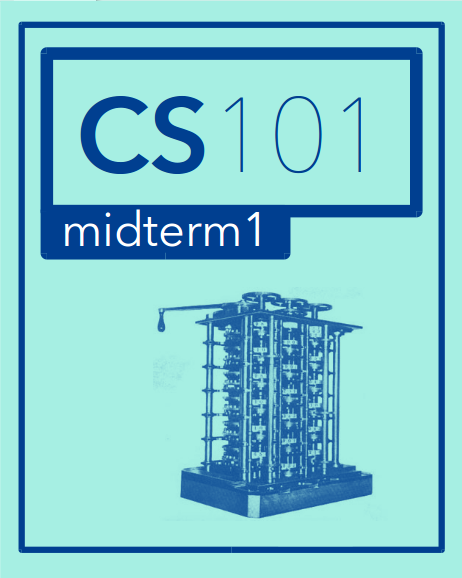
\includegraphics[width=2in]{../img/midterm1-header.png}
\end{center}

\bigskip
\noindent
\begin{itemize}
\item \textbf{Be sure to enter your \underline{NetID} and \underline{the code below} on your Scantron}.
\item Do not turn this page until instructed to do so.
\item There are 30 questions, worth 1 point each.
\item Each question has only \textbf{one} correct answer.
\item You must not communicate with other students during this test.
\item No books, notes, or electronic devices are permitted.
\item This is a 60-minute exam.
\item There are several different versions of this exam.
\end{itemize}

\bigskip\bigskip
\noindent
\textbf{\Large 1. Fill in your information:}

\bigskip
{\Large\bf
\begin{tabular}{ll}
Full Name: & \underbar{\hskip 8cm} \\[0.5em]
UIN (Student Number): & \underbar{\hskip 8cm} \\[0.5em]
NetID: & \underbar{\hskip 8cm}
\end{tabular}
}

\bigskip
\bigskip
\noindent
\textbf{\Large 2. Fill in the following answers on the Scantron form:}

%%%%%%%%%%%%%%%%%%%%%%%%%%%%%%%%%%%%%%%%%%%%%%%%%%%%%%%%%
%%%%%%%%%%%%%%%%%%%%%%%%%%%%%%%%%%%%%%%%%%%%%%%%%%%%%%%%%

\begin{enumerate}
\item[92.] D
\item[93.] D
\item[94.] B
\item[95.] A
\item[96.] E
\end{enumerate}

\newpage

% Zone 1


%%%%%%%%%%%%%%%%%%%%%%%%%%%%%%%%%%%%%%%%%%%%%%%%%%%%%%%%%



\newpage
\noindent
1. (1 point)
Consider the following incomplete program.
\begin{verbatim}
sum=0
???:
    sum=sum+i

\end{verbatim}
The program is intended to sum all of the integers between 1 and 100 (inclusive). What should replace the three question marks to complete the program?


\begin{enumerate}
\item[(A)]
\begin{verbatim}while i<=100 \end{verbatim}

\item[(B)]
\begin{verbatim}while i in range(100)\end{verbatim}

\item[(C)] $\bigstar$ 
\begin{verbatim}for i in range(1,101) \end{verbatim}

\item[(D)]
\begin{verbatim}for i in range(0,100)\end{verbatim}

\end{enumerate}

\vspace*{2em}
\hrule
\vspace{2em}

\noindent {\bf Solution.} 
\vspace{2em}
\hrule height 2pt


\newpage
\noindent
2. (1 point)
Consider the following incomplete function.
\begin{verbatim}
def ismultiple(m,n):
    if ???:
        return False
    else:
        return True
\end{verbatim}
The function is intended to return True if the input parameter m is a multiple of parameter n and False otherwise. For example, \verb|ismultiple(4,2)| should return \verb|True|, but \verb|ismultiple(5,3)| should return \verb|False|. What should replace the three question marks to complete the function?


\begin{enumerate}
\item[(A)]
\begin{verbatim}(n // m) == 0 \end{verbatim}

\item[(B)]
\begin{verbatim}(n % m) == 0 \end{verbatim}

\item[(C)] $\bigstar$ 
\begin{verbatim}(m % n) != 0 \end{verbatim}

\item[(D)]
\begin{verbatim}(m // n) != 0 \end{verbatim}

\end{enumerate}

\vspace*{2em}
\hrule
\vspace{2em}

\noindent {\bf Solution.} 
\vspace{2em}
\hrule height 2pt


\newpage
\noindent
3. (1 point)
How can the following mathematical equation be implemented as a Python expression? Assume \verb|a|, \verb|b|, and \verb|sin| have already been defined.
$$a \sin(a^b - b)$$


\begin{enumerate}
\item[(A)] $\bigstar$ 
\begin{verbatim}a*sin(a**b - b)\end{verbatim}

\item[(B)]
\begin{verbatim}a sin(a**b - b)\end{verbatim}

\item[(C)]
\begin{verbatim}a*sin(a^b - b)\end{verbatim}

\item[(D)]
None of the other answers are correct.

\item[(E)]
\begin{verbatim}a*sin(b^a - b)\end{verbatim}

\end{enumerate}

\vspace*{2em}
\hrule
\vspace{2em}

\noindent {\bf Solution.} 
\vspace{2em}
\hrule height 2pt


\newpage
\noindent
4. (1 point)
Consider the following program:
\begin{verbatim}
x=0
for i in range(4,10):
    if i%3==0:
        x+=3
    elif i%2==0:
        x+=2
    else:
        x+=1
\end{verbatim}
What is the \textbf{value} of \texttt{x} after this program is executed?


\begin{enumerate}
\item[(A)] $\bigstar$ 
\begin{verbatim}12\end{verbatim}

\item[(B)]
\begin{verbatim}13\end{verbatim}

\item[(C)]
\begin{verbatim}11\end{verbatim}

\item[(D)]
\begin{verbatim}14\end{verbatim}

\item[(E)]
\begin{verbatim}10\end{verbatim}

\end{enumerate}

\vspace*{2em}
\hrule
\vspace{2em}

\noindent {\bf Solution.} 
\vspace{2em}
\hrule height 2pt


\newpage
\noindent
5. (1 point)
What is the result of the following expression?
\begin{verbatim}
[ 1, 2, 3 ] * 3.0
\end{verbatim}


\begin{enumerate}
\item[(A)]
\begin{verbatim}[1.0, 2.0, 3.0, 1.0, 2.0, 3.0, 1.0, 2.0, 3.0]\end{verbatim}

\item[(B)]
\begin{verbatim}[3, 6, 9]\end{verbatim}

\item[(C)]
\begin{verbatim}None of the above.\end{verbatim}

\item[(D)]
\begin{verbatim}[3.0, 6.0, 9.0]\end{verbatim}

\item[(E)] $\bigstar$ 
\begin{verbatim}[1, 2, 3, 1, 2, 3, 1, 2, 3]\end{verbatim}

\end{enumerate}

\vspace*{2em}
\hrule
\vspace{2em}

\noindent {\bf Solution.} 
\vspace{2em}
\hrule height 2pt


\newpage
\noindent
6. (1 point)
Consider the following program:
\begin{verbatim}
i=3
x=2
while i < 7:
    x+=i
    i+=2
\end{verbatim}
What is the \textbf{value} of \texttt{x} after this program is executed?


\begin{enumerate}
\item[(A)] $\bigstar$ 
\begin{verbatim}10\end{verbatim}

\item[(B)]
\begin{verbatim}14\end{verbatim}

\item[(C)]
\begin{verbatim}11\end{verbatim}

\item[(D)]
\begin{verbatim}13\end{verbatim}

\item[(E)]
\begin{verbatim}12\end{verbatim}

\end{enumerate}

\vspace*{2em}
\hrule
\vspace{2em}

\noindent {\bf Solution.} 
\vspace{2em}
\hrule height 2pt


\newpage
\noindent
7. (1 point)
Consider the following program.
\begin{verbatim}
x=1
i=0
while(x*x)<=9:
    i=i+(x*x)
    x=x+1
\end{verbatim}
After it is run, what is the final \textbf{value} of \texttt{x}?


\begin{enumerate}
\item[(A)] $\bigstar$ 
\begin{verbatim}4\end{verbatim}

\item[(B)]
\begin{verbatim}30\end{verbatim}

\item[(C)]
\begin{verbatim}14\end{verbatim}

\item[(D)]
\begin{verbatim}5\end{verbatim}

\item[(E)]
\begin{verbatim}3\end{verbatim}

\end{enumerate}

\vspace*{2em}
\hrule
\vspace{2em}

\noindent {\bf Solution.} 
\vspace{2em}
\hrule height 2pt


\newpage
\noindent
8. (1 point)
Consider the following program:
\begin{verbatim}
x=[1,2,3,4,5,6,7,8,9]
x=x[2:-2]
i=1
while i < 3:
    x[i]+=1
    i+=1
\end{verbatim}
What is the \textbf{value} of \texttt{x} after this program is executed?


\begin{enumerate}
\item[(A)]
\begin{verbatim}[3, 5, 6, 6]\end{verbatim}

\item[(B)]
\begin{verbatim}[2, 4, 5, 6, 6, 7]\end{verbatim}

\item[(C)]
\begin{verbatim}[2, 4, 5, 5, 6, 7]\end{verbatim}

\item[(D)] $\bigstar$ 
\begin{verbatim}[3, 5, 6, 6, 7]\end{verbatim}

\item[(E)]
\begin{verbatim}[3, 5, 6, 6, 7, 8]\end{verbatim}

\end{enumerate}

\vspace*{2em}
\hrule
\vspace{2em}

\noindent {\bf Solution.} 
\vspace{2em}
\hrule height 2pt


\newpage
\noindent
9. (1 point)
Consider the following program:
\begin{verbatim}
a=["A","C","C","I","O"]
a.sort()
a[0]=a[-1]
x=""
for e in a:
    x=x+e
\end{verbatim}
What is the \textbf{value} of \texttt{x} after this program is executed?


\begin{enumerate}
\item[(A)] $\bigstar$ 
\begin{verbatim}"OCCIO"\end{verbatim}

\item[(B)]
None of the other answers are correct.

\item[(C)]
\begin{verbatim}"ACCIA"\end{verbatim}

\item[(D)]
\begin{verbatim}"ACCOA"\end{verbatim}

\item[(E)]
\begin{verbatim}"ICCOI"\end{verbatim}

\end{enumerate}

\vspace*{2em}
\hrule
\vspace{2em}

\noindent {\bf Solution.} 
\vspace{2em}
\hrule height 2pt


\newpage
\noindent
10. (1 point)
Evaluate the following expression:
\begin{verbatim}
len("ABCD"[0:3])
\end{verbatim}
What value is produced?


\begin{enumerate}
\item[(A)]
1

\item[(B)] $\bigstar$ 
3

\item[(C)]
2

\item[(D)]
4

\end{enumerate}

\vspace*{2em}
\hrule
\vspace{2em}

\noindent {\bf Solution.} 
\vspace{2em}
\hrule height 2pt


\newpage
\noindent
11. (1 point)
Consider the following program:
\begin{verbatim}
pi="3.14159"
e="2.71828"
x=pi*len(e)+pi
\end{verbatim}
What is the \textbf{type} of \texttt{x} after this program is executed?


\begin{enumerate}
\item[(A)] $\bigstar$ 
\begin{verbatim}String\end{verbatim}

\item[(B)]
\begin{verbatim}Float\end{verbatim}

\item[(C)]
\begin{verbatim}Boolean\end{verbatim}

\item[(D)]
\begin{verbatim}None\end{verbatim}

\item[(E)]
\begin{verbatim}Integer\end{verbatim}

\end{enumerate}

\vspace*{2em}
\hrule
\vspace{2em}

\noindent {\bf Solution.} 
\vspace{2em}
\hrule height 2pt


\newpage
\noindent
12. (1 point)
Consider the following program:
\begin{verbatim}
def fix(s):
    a=list(s)
    a.sort()
    return ''.join(a)

x=["one","two","eleven","twelve"]
s1=fix(x[0]+x[-1])
s2=fix(x[1]+x[-2])

if s1==s2:
    x.sort()
elif s1<s2:
    x.reverse()
else:
    x.append("six")
\end{verbatim}
What is the \textbf{value} of \texttt{x} after this program is executed?


\begin{enumerate}
\item[(A)]
\begin{verbatim}['twelve', 'eleven', 'two', 'one']\end{verbatim}

\item[(B)]
\begin{verbatim}['one', 'two', 'eleven', 'twelve', 'six']\end{verbatim}

\item[(C)]
\begin{verbatim}['one', 'two', 'eleven', 'twelve']\end{verbatim}

\item[(D)] $\bigstar$ 
\begin{verbatim}['eleven', 'one', 'twelve', 'two']\end{verbatim}

\item[(E)]
\begin{verbatim}['two', 'twelve', 'one', 'eleven', 'six']\end{verbatim}

\end{enumerate}

\vspace*{2em}
\hrule
\vspace{2em}

\noindent {\bf Solution.} 
\vspace{2em}
\hrule height 2pt


\newpage
\noindent
13. (1 point)
Consider the following program.
\begin{verbatim}
s="BBCAA"
x=0
y=len(s)-1
while s[x]!=s[y] and x<len(s):
    x+=1
    y-=1
\end{verbatim}
After it is run, what is the final \textbf{value} of \texttt{x}?


\begin{enumerate}
\item[(A)]
\begin{verbatim}0\end{verbatim}

\item[(B)] $\bigstar$ 
\begin{verbatim}2\end{verbatim}

\item[(C)]
\begin{verbatim}3\end{verbatim}

\item[(D)]
\begin{verbatim}4\end{verbatim}

\item[(E)]
\begin{verbatim}1\end{verbatim}

\end{enumerate}

\vspace*{2em}
\hrule
\vspace{2em}

\noindent {\bf Solution.} 
\vspace{2em}
\hrule height 2pt


\newpage
\noindent
14. (1 point)
Consider the following program:
\begin{verbatim}
s="ECTOR"
t="GAWAIN"
x=(len(s)/(len(t)-1))+1
\end{verbatim}
What is the \textbf{type} of \texttt{x} after this program is executed?


\begin{enumerate}
\item[(A)] $\bigstar$ 
\begin{verbatim}Float\end{verbatim}

\item[(B)]
\begin{verbatim}Integer\end{verbatim}

\item[(C)]
\begin{verbatim}String\end{verbatim}

\item[(D)]
\begin{verbatim}None\end{verbatim}

\item[(E)]
\begin{verbatim}Boolean\end{verbatim}

\end{enumerate}

\vspace*{2em}
\hrule
\vspace{2em}

\noindent {\bf Solution.} 
\vspace{2em}
\hrule height 2pt


\newpage
\noindent
15. (1 point)
Consider the following program:
\begin{verbatim}
s="Hobbes"
i=0
x=-1
while i<len(s):
    if s[i]=='b':
        x=i
    i+=1
\end{verbatim}
What is the \textbf{value} of \texttt{x} after this program is executed?


\begin{enumerate}
\item[(A)]
\begin{verbatim}2\end{verbatim}

\item[(B)] $\bigstar$ 
\begin{verbatim}3\end{verbatim}

\item[(C)]
\begin{verbatim}5\end{verbatim}

\item[(D)]
\begin{verbatim}4\end{verbatim}

\item[(E)]
\begin{verbatim}-1\end{verbatim}

\end{enumerate}

\vspace*{2em}
\hrule
\vspace{2em}

\noindent {\bf Solution.} 
\vspace{2em}
\hrule height 2pt


\newpage
\noindent
16. (1 point)
Consider the following program:
\begin{verbatim}
x=3
a=7
if (a%3)==2:
    x=x**2
elif(a%3)==1:
    x=x**1
else:
    x=x**0
\end{verbatim}
What is the \textbf{value} of \texttt{x} after this program is executed?


\begin{enumerate}
\item[(A)]
\begin{verbatim}9\end{verbatim}

\item[(B)]
\begin{verbatim}1\end{verbatim}

\item[(C)] $\bigstar$ 
\begin{verbatim}3\end{verbatim}

\item[(D)]
None of the other answers are correct.

\item[(E)]
\begin{verbatim}7\end{verbatim}

\end{enumerate}

\vspace*{2em}
\hrule
\vspace{2em}

\noindent {\bf Solution.} 
\vspace{2em}
\hrule height 2pt


\newpage
\noindent
17. (1 point)
Consider the following program:
\begin{verbatim}
x=[1,2,3]
def f(a):
    s=""
    a.append(4)
    for i in a:
        s+=str(i)
    return s

x.append(f(x))
\end{verbatim}
What is the \textbf{value} of \texttt{x} after this program is executed?


\begin{enumerate}
\item[(A)]
\begin{verbatim}[1, 2, 3]\end{verbatim}

\item[(B)] $\bigstar$ 
\begin{verbatim}[1, 2, 3, 4, '1234']\end{verbatim}

\item[(C)]
\begin{verbatim}[1, 2, 3, 10]\end{verbatim}

\item[(D)]
\begin{verbatim}[1, 2, 3, '1234']\end{verbatim}

\item[(E)]
\begin{verbatim}[1, 2, 3, '123']\end{verbatim}

\end{enumerate}

\vspace*{2em}
\hrule
\vspace{2em}

\noindent {\bf Solution.} 
\vspace{2em}
\hrule height 2pt


\newpage
\noindent
18. (1 point)
Consider the following program.
\begin{verbatim}
kay = 2
wart = 3

def knight(kay,wart):
    wart += 2
    kay += 3
    return wart + kay

kay = knight(wart, kay) + knight(kay, wart)
\end{verbatim}
After it is run, what is the final \textbf{value} of \texttt{kay}?


\begin{enumerate}
\item[(A)]
\begin{verbatim}5\end{verbatim}

\item[(B)]
\begin{verbatim}2\end{verbatim}

\item[(C)]
\begin{verbatim}3\end{verbatim}

\item[(D)] $\bigstar$ 
None of the other answers are correct.

\end{enumerate}

\vspace*{2em}
\hrule
\vspace{2em}

\noindent {\bf Solution.} 
\vspace{2em}
\hrule height 2pt


\newpage
\noindent
19. (1 point)
Consider the following program:
\begin{verbatim}
a=3
b=4
if a!=b:
    a=b
elif a==4:
    a=5
else:
    b=a
\end{verbatim}
What is the \textbf{value} of a after this program is executed?


\begin{enumerate}
\item[(A)]
None of the other answers are correct.

\item[(B)]
\begin{verbatim}7\end{verbatim}

\item[(C)]
\begin{verbatim}3\end{verbatim}

\item[(D)] $\bigstar$ 
\begin{verbatim}4\end{verbatim}

\item[(E)]
\begin{verbatim}5\end{verbatim}

\end{enumerate}

\vspace*{2em}
\hrule
\vspace{2em}

\noindent {\bf Solution.} 
\vspace{2em}
\hrule height 2pt


\newpage
\noindent
20. (1 point)
Consider the following program:
\begin{verbatim}
s="G+R+A+I+L"
x=s.split("+")[1:-2]
\end{verbatim}
What is the \textbf{value} of \texttt{x} after this program is executed?


\begin{enumerate}
\item[(A)]
\begin{verbatim}3\end{verbatim}

\item[(B)]
\begin{verbatim}'RAI'\end{verbatim}

\item[(C)]
\begin{verbatim}None\end{verbatim}

\item[(D)]
\begin{verbatim}False\end{verbatim}

\item[(E)] $\bigstar$ 
\begin{verbatim}['R','A']\end{verbatim}

\end{enumerate}

\vspace*{2em}
\hrule
\vspace{2em}

\noindent {\bf Solution.} 
\vspace{2em}
\hrule height 2pt


\newpage
\noindent
21. (1 point)
Consider the following program.
\begin{verbatim}
x=[]
for j in range(0,5):
    if (j%3)==0:
        x.append("-")
    if (j%4)==0:
        x.append("*")
\end{verbatim}
After it is run, what is the final \textbf{value} of \texttt{x}?


\begin{enumerate}
\item[(A)] $\bigstar$ 
\begin{verbatim}["-","*","-","*"]\end{verbatim}

\item[(B)]
\begin{verbatim}["*","-","*"]\end{verbatim}

\item[(C)]
\begin{verbatim}["-","*"]\end{verbatim}

\item[(D)]
\begin{verbatim}["*","-","*"]\end{verbatim}

\item[(E)]
None of the other answers are correct.

\end{enumerate}

\vspace*{2em}
\hrule
\vspace{2em}

\noindent {\bf Solution.} 
\vspace{2em}
\hrule height 2pt


\newpage
\noindent
22. (1 point)
Consider the following Python program.
\begin{verbatim}
e=[1,3,5,7,9,11]
d=[0,0,0]
for i in range(0,len(e)):
    d[i%3]+=e[i]
x=d[2]
\end{verbatim}
After it is run, what is the final \textbf{value} of \texttt{x}?


\begin{enumerate}
\item[(A)]
\begin{verbatim}8\end{verbatim}

\item[(B)]
\begin{verbatim}7\end{verbatim}

\item[(C)]
\begin{verbatim}12\end{verbatim}

\item[(D)]
\begin{verbatim}0\end{verbatim}

\item[(E)] $\bigstar$ 
\begin{verbatim}16\end{verbatim}

\end{enumerate}

\vspace*{2em}
\hrule
\vspace{2em}

\noindent {\bf Solution.} 
\vspace{2em}
\hrule height 2pt


\newpage
\noindent
23. (1 point)
Consider the following program:
\begin{verbatim}
x="KING ARTHUR-MORGANA LEFAY-SIR BEDIVERE".split("-")
y=x
y.reverse()
\end{verbatim}
What is the \textbf{value} of \texttt{x} after this program is executed?


\begin{enumerate}
\item[(A)]
\begin{verbatim}['KING', 'ARTHUR-MORGANA', 'LEFAY-SIR', 'BEDIVERE']\end{verbatim}

\item[(B)] $\bigstar$ 
\begin{verbatim}['SIR BEDIVERE', 'MORGANA LEFAY', 'KING ARTHUR']\end{verbatim}

\item[(C)]
\begin{verbatim}['KING ARTHUR', 'MORGANA LEFAY', 'SIR BEDIVERE']\end{verbatim}

\item[(D)]
\begin{verbatim}None\end{verbatim}

\item[(E)]
\begin{verbatim}['BEDIVERE', 'LEFAY-SIR', 'ARTHUR-MORGANA', 'KING']\end{verbatim}

\end{enumerate}

\vspace*{2em}
\hrule
\vspace{2em}

\noindent {\bf Solution.} 
\vspace{2em}
\hrule height 2pt


\newpage
\noindent
24. (1 point)
Consider the following program:
\begin{verbatim}
x=str(1.2)*2
\end{verbatim}
What is the \textbf{value} of \texttt{x} after this program is executed?


\begin{enumerate}
\item[(A)] $\bigstar$ 
\begin{verbatim}"1.21.2"\end{verbatim}

\item[(B)]
None of the other answers are correct.

\item[(C)]
\begin{verbatim}2.4\end{verbatim}

\item[(D)]
\begin{verbatim}"2.4"\end{verbatim}

\item[(E)]
\begin{verbatim}"1.2*2"\end{verbatim}

\end{enumerate}

\vspace*{2em}
\hrule
\vspace{2em}

\noindent {\bf Solution.} 
\vspace{2em}
\hrule height 2pt


\newpage
\noindent
25. (1 point)
Evaluate the following expression:
\begin{verbatim}
[1,2]*len("3")
\end{verbatim}
What value is produced?


\begin{enumerate}
\item[(A)]
\begin{verbatim}[1,2,3]\end{verbatim}

\item[(B)] $\bigstar$ 
\begin{verbatim}[1,2]\end{verbatim}

\item[(C)]
\begin{verbatim}[1,2,1,2,1,2]\end{verbatim}

\item[(D)]
\begin{verbatim}[1,2,1]\end{verbatim}

\end{enumerate}

\vspace*{2em}
\hrule
\vspace{2em}

\noindent {\bf Solution.} 
\vspace{2em}
\hrule height 2pt


\newpage
\noindent
26. (1 point)
Consider the following incomplete Python program.
\begin{verbatim}
s="".join(["1","0","2","1"])
x=0
for i in range(len(s)-1):
    x+=int(???)
\end{verbatim}
What should replace the three question marks so the resulting value of \texttt{x} is 33?


\begin{enumerate}
\item[(A)]
\begin{verbatim}s[i:i-1]\end{verbatim}

\item[(B)] $\bigstar$ 
\begin{verbatim}s[i:i+2]\end{verbatim}

\item[(C)]
\begin{verbatim}s[i:i+1]\end{verbatim}

\item[(D)]
\begin{verbatim}s[i+1:i+2]\end{verbatim}

\end{enumerate}

\vspace*{2em}
\hrule
\vspace{2em}

\noindent {\bf Solution.} 
\vspace{2em}
\hrule height 2pt


\newpage
\noindent
27. (1 point)
Consider the following program:
\begin{verbatim}
s="TRIS %i"
t="ISEU"
x=s % len(t)
\end{verbatim}
What is the \textbf{type} of \texttt{x} after this program is executed?


\begin{enumerate}
\item[(A)]
\begin{verbatim}Float\end{verbatim}

\item[(B)]
\begin{verbatim}None\end{verbatim}

\item[(C)]
\begin{verbatim}Boolean\end{verbatim}

\item[(D)]
\begin{verbatim}Integer\end{verbatim}

\item[(E)] $\bigstar$ 
\begin{verbatim}String\end{verbatim}

\end{enumerate}

\vspace*{2em}
\hrule
\vspace{2em}

\noindent {\bf Solution.} 
\vspace{2em}
\hrule height 2pt


\newpage
\noindent
28. (1 point)
Consider the following program.
\begin{verbatim}
def artificing(s):
    return s*2
    return s+"%i" % 2
    return s

s=artificing("MERLIN")
\end{verbatim}
After it is run, what is the final \textbf{value} of s?


\begin{enumerate}
\item[(A)]
\begin{verbatim}None\end{verbatim}

\item[(B)]
\begin{verbatim}"MERLIN"\end{verbatim}

\item[(C)]
\begin{verbatim}"MERLIN2"\end{verbatim}

\item[(D)] $\bigstar$ 
\begin{verbatim}"MERLINMERLIN"\end{verbatim}

\item[(E)]
\begin{verbatim}12\end{verbatim}

\end{enumerate}

\vspace*{2em}
\hrule
\vspace{2em}

\noindent {\bf Solution.} 
\vspace{2em}
\hrule height 2pt


\newpage
\noindent
29. (1 point)
For this problem, you should compose a function which accomplishes a given task using the available code blocks arranged in the correct functional order.  \emph{We ignore indentation for this problem.}

\texttt{find\_max} should accept a \texttt{list} and return the value of the maximum item in the \texttt{list}.  (\texttt{None} is always the lowest value in any numeric comparison, so you may use it as an initializer.)

\begin{verbatim}
def find_max(my_list):
\end{verbatim}

\begin{enumerate}[1]
\item \texttt{max\_val = i}
\item \texttt{max\_val = None}
\item \texttt{for i in range(len(my\_list)):}
\item \texttt{if i > max\_val:}
\item \texttt{max\_val = my\_list[i]}
\item \texttt{return max\_val}
\item \texttt{for i in range(my\_list):}
\item \texttt{if my\_list[i] > max\_val:}
\item \texttt{print(max\_val)}
\end{enumerate}



\begin{enumerate}
\item[(A)]
2, 3, 4, 1, 6

\item[(B)]
3, 2, 8, 5, 9

\item[(C)]
2, 3, 8, 1, 6

\item[(D)]
2, 7, 4, 5, 6

\item[(E)] $\bigstar$ 
2, 3, 8, 5, 6

\end{enumerate}

\vspace*{2em}
\hrule
\vspace{2em}

\noindent {\bf Solution.} 
\vspace{2em}
\hrule height 2pt


\newpage
\noindent
30. (1 point)
Consider the following program:
\begin{verbatim}
a=["merlin","sir agravaine","king pellinore"]
b=[ ]
for i in range(0,3):
    b.append(a[0-i].title())
\end{verbatim}
What is the \textbf{value} of b after this program is executed?


\begin{enumerate}
\item[(A)] $\bigstar$ 
\begin{verbatim}['Merlin', 'King Pellinore', 'Sir Agravaine']\end{verbatim}

\item[(B)]
\begin{verbatim}[ ]\end{verbatim}

\item[(C)]
\begin{verbatim}['King Pellinore', 'Sir Agravaine', 'Merlin']\end{verbatim}

\item[(D)]
\begin{verbatim}['King Pellinore', 'Sir Agravaine']\end{verbatim}

\item[(E)]
\begin{verbatim}['Sir Agravaine', 'King Pellinore']\end{verbatim}

\end{enumerate}

\vspace*{2em}
\hrule
\vspace{2em}

\noindent {\bf Solution.} 
\vspace{2em}
\hrule height 2pt

%%%%%%%%%%%%%%%%%%%%%%%%%%%%%%%%%%%%%%%%%%%%%%%%%%%%%%%%%%%%%%%%%%%%%%
%%%%%%%%%%%%%%%%%%%%%%%%%%%%%%%%%%%%%%%%%%%%%%%%%%%%%%%%%%%%%%%%%%%%%%
%%%%%%%%%%%%%%%%%%%%%%%%%%%%%%%%%%%%%%%%%%%%%%%%%%%%%%%%%%%%%%%%%%%%%%
%%%%%%%%%%%%%%%%%%%%%%%%%%%%%%%%%%%%%%%%%%%%%%%%%%%%%%%%%%%%%%%%%%%%%%
% Exam number 45

\message{Exam 45/50}
\cleardoublepage
\setcounter{page}{1}


\begin{center}
%\textbf{\Large CS 101 Midterm \#1}
%
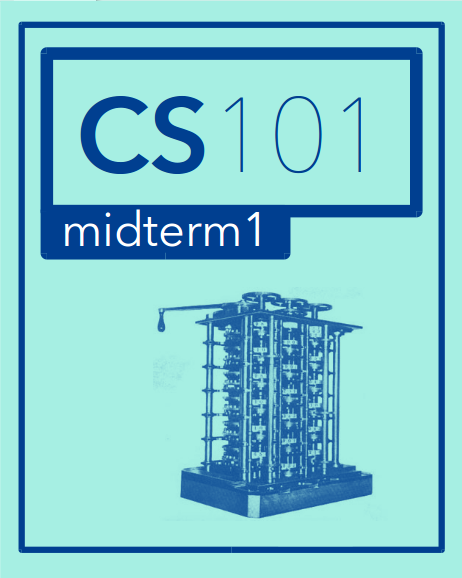
\includegraphics[width=2in]{../img/midterm1-header.png}
\end{center}

\bigskip
\noindent
\begin{itemize}
\item \textbf{Be sure to enter your \underline{NetID} and \underline{the code below} on your Scantron}.
\item Do not turn this page until instructed to do so.
\item There are 30 questions, worth 1 point each.
\item Each question has only \textbf{one} correct answer.
\item You must not communicate with other students during this test.
\item No books, notes, or electronic devices are permitted.
\item This is a 60-minute exam.
\item There are several different versions of this exam.
\end{itemize}

\bigskip\bigskip
\noindent
\textbf{\Large 1. Fill in your information:}

\bigskip
{\Large\bf
\begin{tabular}{ll}
Full Name: & \underbar{\hskip 8cm} \\[0.5em]
UIN (Student Number): & \underbar{\hskip 8cm} \\[0.5em]
NetID: & \underbar{\hskip 8cm}
\end{tabular}
}

\bigskip
\bigskip
\noindent
\textbf{\Large 2. Fill in the following answers on the Scantron form:}

%%%%%%%%%%%%%%%%%%%%%%%%%%%%%%%%%%%%%%%%%%%%%%%%%%%%%%%%%
%%%%%%%%%%%%%%%%%%%%%%%%%%%%%%%%%%%%%%%%%%%%%%%%%%%%%%%%%

\begin{enumerate}
\item[92.] E
\item[93.] D
\item[94.] B
\item[95.] B
\item[96.] A
\end{enumerate}

\newpage

% Zone 1


%%%%%%%%%%%%%%%%%%%%%%%%%%%%%%%%%%%%%%%%%%%%%%%%%%%%%%%%%



\newpage
\noindent
1. (1 point)
Consider the following program:
\begin{verbatim}
pi="3.14159"
e="2.71828"
x=pi in pi*len(e)
\end{verbatim}
What is the \textbf{type} of \texttt{x} after this program is executed?


\begin{enumerate}
\item[(A)]
\begin{verbatim}None\end{verbatim}

\item[(B)]
\begin{verbatim}Integer\end{verbatim}

\item[(C)] $\bigstar$ 
\begin{verbatim}Boolean\end{verbatim}

\item[(D)]
\begin{verbatim}String\end{verbatim}

\item[(E)]
\begin{verbatim}Float\end{verbatim}

\end{enumerate}

\vspace*{2em}
\hrule
\vspace{2em}

\noindent {\bf Solution.} 
\vspace{2em}
\hrule height 2pt


\newpage
\noindent
2. (1 point)
Consider the following program.
\begin{verbatim}
s="ABCBA"
x=0
y=len(s)-1
while s[x]==s[y] and x<y:
    x+=1
    y-=1
\end{verbatim}
After it is run, what is the final \textbf{value} of \texttt{x}?


\begin{enumerate}
\item[(A)] $\bigstar$ 
\begin{verbatim}2\end{verbatim}

\item[(B)]
\begin{verbatim}4\end{verbatim}

\item[(C)]
\begin{verbatim}3\end{verbatim}

\item[(D)]
\begin{verbatim}0\end{verbatim}

\item[(E)]
\begin{verbatim}1\end{verbatim}

\end{enumerate}

\vspace*{2em}
\hrule
\vspace{2em}

\noindent {\bf Solution.} 
\vspace{2em}
\hrule height 2pt


\newpage
\noindent
3. (1 point)
Consider the following program:
\begin{verbatim}
x=[1,2,3,4,5,6,7,8,9]
x=x[2:-2]
i=1
while i < 3:
    x[i]+=1
    i+=1
\end{verbatim}
What is the \textbf{value} of \texttt{x} after this program is executed?


\begin{enumerate}
\item[(A)]
\begin{verbatim}[3, 5, 6, 6, 7, 8]\end{verbatim}

\item[(B)]
\begin{verbatim}[2, 4, 5, 6, 6, 7]\end{verbatim}

\item[(C)] $\bigstar$ 
\begin{verbatim}[3, 5, 6, 6, 7]\end{verbatim}

\item[(D)]
\begin{verbatim}[3, 5, 6, 6]\end{verbatim}

\item[(E)]
\begin{verbatim}[2, 4, 5, 5, 6, 7]\end{verbatim}

\end{enumerate}

\vspace*{2em}
\hrule
\vspace{2em}

\noindent {\bf Solution.} 
\vspace{2em}
\hrule height 2pt


\newpage
\noindent
4. (1 point)
Evaluate the following expression:
\begin{verbatim}
[1,2]*len("3")
\end{verbatim}
What value is produced?


\begin{enumerate}
\item[(A)]
\begin{verbatim}[1,2,3]\end{verbatim}

\item[(B)] $\bigstar$ 
\begin{verbatim}[1,2]\end{verbatim}

\item[(C)]
\begin{verbatim}[1,2,1]\end{verbatim}

\item[(D)]
\begin{verbatim}[1,2,1,2,1,2]\end{verbatim}

\end{enumerate}

\vspace*{2em}
\hrule
\vspace{2em}

\noindent {\bf Solution.} 
\vspace{2em}
\hrule height 2pt


\newpage
\noindent
5. (1 point)
Consider the following incomplete function.
\begin{verbatim}
def isdivisible(m,n):
    if ???:
        return False
    else:
        return True
\end{verbatim}
The function is intended to return True if the input parameter m is evenly divisible by the parameter n and False otherwise. For example, \verb|isdivisible(4,2)| should return \verb|True|, but \verb|isdivisible(5,3)| should return \verb|False|. What should replace the three question marks to complete the function?


\begin{enumerate}
\item[(A)]
\begin{verbatim}(n // m) == 0 \end{verbatim}

\item[(B)]
\begin{verbatim}(m // n) != 0 \end{verbatim}

\item[(C)]
\begin{verbatim}(n % m) == 0 \end{verbatim}

\item[(D)] $\bigstar$ 
\begin{verbatim}(m % n) != 0 \end{verbatim}

\end{enumerate}

\vspace*{2em}
\hrule
\vspace{2em}

\noindent {\bf Solution.} 
\vspace{2em}
\hrule height 2pt


\newpage
\noindent
6. (1 point)
Evaluate the following expression:
\begin{verbatim}
len("ABCD"[0:3])
\end{verbatim}
What value is produced?


\begin{enumerate}
\item[(A)]
4

\item[(B)]
2

\item[(C)] $\bigstar$ 
3

\item[(D)]
1

\end{enumerate}

\vspace*{2em}
\hrule
\vspace{2em}

\noindent {\bf Solution.} 
\vspace{2em}
\hrule height 2pt


\newpage
\noindent
7. (1 point)
How can the following mathematical equation be implemented as a Python expression? Assume \verb|a|, \verb|b|, and \verb|sin| have already been defined.
$$a \sin(a^b - b)$$


\begin{enumerate}
\item[(A)]
\begin{verbatim}a sin(a**b - b)\end{verbatim}

\item[(B)]
\begin{verbatim}a*sin(a^b - b)\end{verbatim}

\item[(C)]
\begin{verbatim}a*sin(b^a - b)\end{verbatim}

\item[(D)]
None of the other answers are correct.

\item[(E)] $\bigstar$ 
\begin{verbatim}a*sin(a**b - b)\end{verbatim}

\end{enumerate}

\vspace*{2em}
\hrule
\vspace{2em}

\noindent {\bf Solution.} 
\vspace{2em}
\hrule height 2pt


\newpage
\noindent
8. (1 point)
Consider the following program:
\begin{verbatim}
s="-B-O-R-S-"
x=s.split("-")[2:-2]
\end{verbatim}
What is the \textbf{value} of \texttt{x} after this program is executed?


\begin{enumerate}
\item[(A)]
\begin{verbatim}None\end{verbatim}

\item[(B)]
\begin{verbatim}False\end{verbatim}

\item[(C)] $\bigstar$ 
\begin{verbatim}['O', 'R']\end{verbatim}

\item[(D)]
\begin{verbatim}''\end{verbatim}

\item[(E)]
\begin{verbatim}'ORS'\end{verbatim}

\end{enumerate}

\vspace*{2em}
\hrule
\vspace{2em}

\noindent {\bf Solution.} 
\vspace{2em}
\hrule height 2pt


\newpage
\noindent
9. (1 point)
Consider the following program.
\begin{verbatim}
x=[]
for j in range(0,5):
    if (j%3)==0:
        x.append("-")
    if (j%4)==0:
        x.append("*")
\end{verbatim}
After it is run, what is the final \textbf{value} of \texttt{x}?


\begin{enumerate}
\item[(A)] $\bigstar$ 
\begin{verbatim}["-","*","-","*"]\end{verbatim}

\item[(B)]
\begin{verbatim}["-","*"]\end{verbatim}

\item[(C)]
\begin{verbatim}["*","-","*"]\end{verbatim}

\item[(D)]
None of the other answers are correct.

\item[(E)]
\begin{verbatim}["*","-","*"]\end{verbatim}

\end{enumerate}

\vspace*{2em}
\hrule
\vspace{2em}

\noindent {\bf Solution.} 
\vspace{2em}
\hrule height 2pt


\newpage
\noindent
10. (1 point)
Consider the following program.
\begin{verbatim}
def artificing(s):
    return s*2
    return s+"%i" % 2
    return s

s=artificing("MERLIN")
\end{verbatim}
After it is run, what is the final \textbf{value} of s?


\begin{enumerate}
\item[(A)]
\begin{verbatim}12\end{verbatim}

\item[(B)] $\bigstar$ 
\begin{verbatim}"MERLINMERLIN"\end{verbatim}

\item[(C)]
\begin{verbatim}None\end{verbatim}

\item[(D)]
\begin{verbatim}"MERLIN"\end{verbatim}

\item[(E)]
\begin{verbatim}"MERLIN2"\end{verbatim}

\end{enumerate}

\vspace*{2em}
\hrule
\vspace{2em}

\noindent {\bf Solution.} 
\vspace{2em}
\hrule height 2pt


\newpage
\noindent
11. (1 point)
Consider the following program:
\begin{verbatim}
i=2
x=3
while i < 7:
    x+=i
    i+=2
\end{verbatim}
What is the \textbf{value} of \texttt{x} after this program is executed?


\begin{enumerate}
\item[(A)]
\begin{verbatim}12\end{verbatim}

\item[(B)] $\bigstar$ 
\begin{verbatim}15\end{verbatim}

\item[(C)]
\begin{verbatim}11\end{verbatim}

\item[(D)]
\begin{verbatim}13\end{verbatim}

\item[(E)]
\begin{verbatim}14\end{verbatim}

\end{enumerate}

\vspace*{2em}
\hrule
\vspace{2em}

\noindent {\bf Solution.} 
\vspace{2em}
\hrule height 2pt


\newpage
\noindent
12. (1 point)
Consider the following incomplete Python program.
\begin{verbatim}
s="".join(["2","2","0","1"])
x=0
for i in range(len(s)-1):
    x+=int(???)
\end{verbatim}
What should replace the three question marks so the resulting value of \texttt{x} is 43?


\begin{enumerate}
\item[(A)]
\begin{verbatim}s[i+1:i+2]\end{verbatim}

\item[(B)]
\begin{verbatim}s[i:i-1]\end{verbatim}

\item[(C)] $\bigstar$ 
\begin{verbatim}s[i:i+2]\end{verbatim}

\item[(D)]
\begin{verbatim}s[i:i+1]\end{verbatim}

\end{enumerate}

\vspace*{2em}
\hrule
\vspace{2em}

\noindent {\bf Solution.} 
\vspace{2em}
\hrule height 2pt


\newpage
\noindent
13. (1 point)
Consider the following program:
\begin{verbatim}
s="ECTOR"
t="GAWAIN"
x=len(str(s.isupper()))-t.find("A")
\end{verbatim}
What is the \textbf{type} of \texttt{x} after this program is executed?


\begin{enumerate}
\item[(A)]
\begin{verbatim}Float\end{verbatim}

\item[(B)]
\begin{verbatim}String\end{verbatim}

\item[(C)] $\bigstar$ 
\begin{verbatim}Integer\end{verbatim}

\item[(D)]
\begin{verbatim}Boolean\end{verbatim}

\item[(E)]
\begin{verbatim}None\end{verbatim}

\end{enumerate}

\vspace*{2em}
\hrule
\vspace{2em}

\noindent {\bf Solution.} 
\vspace{2em}
\hrule height 2pt


\newpage
\noindent
14. (1 point)
Consider the following program:
\begin{verbatim}
s="TRIS %i"
t="ISEU"
x=s % len(t)
\end{verbatim}
What is the \textbf{type} of \texttt{x} after this program is executed?


\begin{enumerate}
\item[(A)] $\bigstar$ 
\begin{verbatim}String\end{verbatim}

\item[(B)]
\begin{verbatim}Boolean\end{verbatim}

\item[(C)]
\begin{verbatim}Integer\end{verbatim}

\item[(D)]
\begin{verbatim}None\end{verbatim}

\item[(E)]
\begin{verbatim}Float\end{verbatim}

\end{enumerate}

\vspace*{2em}
\hrule
\vspace{2em}

\noindent {\bf Solution.} 
\vspace{2em}
\hrule height 2pt


\newpage
\noindent
15. (1 point)
Consider the following program:
\begin{verbatim}
x=0
for i in range(2,8):
    if i%3==0:
        x+=3
    elif i%2==0:
        x+=2
    else:
        x+=1
\end{verbatim}
What is the \textbf{value} of \texttt{x} after this program is executed?


\begin{enumerate}
\item[(A)] $\bigstar$ 
\begin{verbatim}12\end{verbatim}

\item[(B)]
\begin{verbatim}10\end{verbatim}

\item[(C)]
\begin{verbatim}13\end{verbatim}

\item[(D)]
\begin{verbatim}14\end{verbatim}

\item[(E)]
\begin{verbatim}11\end{verbatim}

\end{enumerate}

\vspace*{2em}
\hrule
\vspace{2em}

\noindent {\bf Solution.} 
\vspace{2em}
\hrule height 2pt


\newpage
\noindent
16. (1 point)
\begin{verbatim}
x=str(3)+"str(3)"
\end{verbatim}
What is the \textbf{value} of \texttt{x} after this program is executed?


\begin{enumerate}
\item[(A)]
\begin{verbatim}"333"\end{verbatim}

\item[(B)]
None of the other answers are correct.

\item[(C)]
\begin{verbatim}"33"\end{verbatim}

\item[(D)]
\begin{verbatim}33\end{verbatim}

\item[(E)] $\bigstar$ 
\begin{verbatim}"3str(3)"\end{verbatim}

\end{enumerate}

\vspace*{2em}
\hrule
\vspace{2em}

\noindent {\bf Solution.} 
\vspace{2em}
\hrule height 2pt


\newpage
\noindent
17. (1 point)
Consider the following Python program.
\begin{verbatim}
e=[1,3,5,7,9,11]
d=[0,0,0]
for i in range(0,len(e)):
    d[i%3]+=e[i]
x=d[1]
\end{verbatim}
After it is run, what is the final \textbf{value} of \texttt{x}?


\begin{enumerate}
\item[(A)]
\begin{verbatim}0\end{verbatim}

\item[(B)] $\bigstar$ 
\begin{verbatim}12\end{verbatim}

\item[(C)]
\begin{verbatim}8\end{verbatim}

\item[(D)]
\begin{verbatim}16\end{verbatim}

\item[(E)]
\begin{verbatim}3\end{verbatim}

\end{enumerate}

\vspace*{2em}
\hrule
\vspace{2em}

\noindent {\bf Solution.} 
\vspace{2em}
\hrule height 2pt


\newpage
\noindent
18. (1 point)
Consider the following program:
\begin{verbatim}
a=["merlin","sir agravaine","king pellinore"]
b=[ ]
for i in range(0,4):
    b.append(a[0-i].title())
\end{verbatim}
What is the \textbf{value} of b after this program is executed?


\begin{enumerate}
\item[(A)]
\begin{verbatim}['Merlin', 'King Pellinore', 'Sir Agravaine']\end{verbatim}

\item[(B)]
\begin{verbatim}['King Pellinore', 'Sir Agravaine', 'Merlin']\end{verbatim}

\item[(C)]
\begin{verbatim}[ ]\end{verbatim}

\item[(D)]
\begin{verbatim}['Merlin', 'Sir Agravaine', 'King Pellinore', 'Merlin']\end{verbatim}

\item[(E)] $\bigstar$ 
\begin{verbatim}['Merlin', 'King Pellinore', 'Sir Agravaine', 'Merlin']\end{verbatim}

\end{enumerate}

\vspace*{2em}
\hrule
\vspace{2em}

\noindent {\bf Solution.} 
\vspace{2em}
\hrule height 2pt


\newpage
\noindent
19. (1 point)
Consider the following program.
\begin{verbatim}
x=1
i=0
while(x*x)<=9:
    i=i+(x*x)
    x=x+1
\end{verbatim}
After it is run, what is the final \textbf{value} of \texttt{x}?


\begin{enumerate}
\item[(A)]
\begin{verbatim}5\end{verbatim}

\item[(B)]
\begin{verbatim}3\end{verbatim}

\item[(C)]
\begin{verbatim}30\end{verbatim}

\item[(D)]
\begin{verbatim}14\end{verbatim}

\item[(E)] $\bigstar$ 
\begin{verbatim}4\end{verbatim}

\end{enumerate}

\vspace*{2em}
\hrule
\vspace{2em}

\noindent {\bf Solution.} 
\vspace{2em}
\hrule height 2pt


\newpage
\noindent
20. (1 point)
Consider the following program.
\begin{verbatim}
kay = 2
wart = 3

def knight(kay,wart):
    wart += 2
    kay += 3
    return wart + kay

kay = knight(wart, kay) + knight(kay, wart)
\end{verbatim}
After it is run, what is the final \textbf{value} of \texttt{kay}?


\begin{enumerate}
\item[(A)]
\begin{verbatim}2\end{verbatim}

\item[(B)]
\begin{verbatim}3\end{verbatim}

\item[(C)] $\bigstar$ 
None of the other answers are correct.

\item[(D)]
\begin{verbatim}5\end{verbatim}

\end{enumerate}

\vspace*{2em}
\hrule
\vspace{2em}

\noindent {\bf Solution.} 
\vspace{2em}
\hrule height 2pt


\newpage
\noindent
21. (1 point)
Consider the following program:
\begin{verbatim}
x="KING ARTHUR-MORGANA LEFAY-SIR BEDIVERE".split("-")
y=x[:]
y.reverse()
\end{verbatim}
What is the \textbf{value} of \texttt{x} after this program is executed?


\begin{enumerate}
\item[(A)]
\begin{verbatim}['SIR BEDIVERE', 'MORGANA LEFAY', 'KING ARTHUR']\end{verbatim}

\item[(B)]
\begin{verbatim}['BEDIVERE', 'LEFAY-SIR', 'ARTHUR-MORGANA', 'KING']\end{verbatim}

\item[(C)]
\begin{verbatim}['KING', 'ARTHUR-MORGANA', 'LEFAY-SIR', 'BEDIVERE']\end{verbatim}

\item[(D)]
\begin{verbatim}None\end{verbatim}

\item[(E)] $\bigstar$ 
\begin{verbatim}['KING ARTHUR', 'MORGANA LEFAY', 'SIR BEDIVERE']\end{verbatim}

\end{enumerate}

\vspace*{2em}
\hrule
\vspace{2em}

\noindent {\bf Solution.} 
\vspace{2em}
\hrule height 2pt


\newpage
\noindent
22. (1 point)
Consider the following incomplete program.
\begin{verbatim}
sum=0
for i in range(0,100):
    ???

\end{verbatim}
The program is intended to sum all of the integers between 1 and 100 (inclusive). What should replace the three question marks to complete the program?


\begin{enumerate}
\item[(A)]
\begin{verbatim}sum=sum+1\end{verbatim}

\item[(B)]
\begin{verbatim}sum+1=sum \end{verbatim}

\item[(C)]
\begin{verbatim}sum=sum+i \end{verbatim}

\item[(D)] $\bigstar$ 
\begin{verbatim}sum=sum+i+1 \end{verbatim}

\end{enumerate}

\vspace*{2em}
\hrule
\vspace{2em}

\noindent {\bf Solution.} 
\vspace{2em}
\hrule height 2pt


\newpage
\noindent
23. (1 point)
Consider the following program:
\begin{verbatim}
x=3
a=7
if (a%3)==2:
    x=x**2
elif(a%3)==1:
    x=x**1
else:
    x=x**0
\end{verbatim}
What is the \textbf{value} of \texttt{x} after this program is executed?


\begin{enumerate}
\item[(A)]
\begin{verbatim}7\end{verbatim}

\item[(B)] $\bigstar$ 
\begin{verbatim}3\end{verbatim}

\item[(C)]
\begin{verbatim}1\end{verbatim}

\item[(D)]
\begin{verbatim}9\end{verbatim}

\item[(E)]
None of the other answers are correct.

\end{enumerate}

\vspace*{2em}
\hrule
\vspace{2em}

\noindent {\bf Solution.} 
\vspace{2em}
\hrule height 2pt


\newpage
\noindent
24. (1 point)
Consider the following program:
\begin{verbatim}
a=3
b=4
if a!=b:
    a=b
elif a==4:
    a=5
else:
    b=a
\end{verbatim}
What is the \textbf{value} of a after this program is executed?


\begin{enumerate}
\item[(A)]
\begin{verbatim}5\end{verbatim}

\item[(B)]
\begin{verbatim}3\end{verbatim}

\item[(C)]
None of the other answers are correct.

\item[(D)]
\begin{verbatim}7\end{verbatim}

\item[(E)] $\bigstar$ 
\begin{verbatim}4\end{verbatim}

\end{enumerate}

\vspace*{2em}
\hrule
\vspace{2em}

\noindent {\bf Solution.} 
\vspace{2em}
\hrule height 2pt


\newpage
\noindent
25. (1 point)
What is the result of the following expression?
\begin{verbatim}
[ 1, 2, 3 ] * 3
\end{verbatim}


\begin{enumerate}
\item[(A)]
\begin{verbatim}[3, 6, 9]\end{verbatim}

\item[(B)]
\begin{verbatim}[3.0, 6.0, 9.0]\end{verbatim}

\item[(C)]
\begin{verbatim}(3, 6, 9)\end{verbatim}

\item[(D)]
\begin{verbatim}[1.0, 2.0, 3.0, 1.0, 2.0, 3.0, 1.0, 2.0, 3.0]\end{verbatim}

\item[(E)] $\bigstar$ 
\begin{verbatim}[1, 2, 3, 1, 2, 3, 1, 2, 3]\end{verbatim}

\end{enumerate}

\vspace*{2em}
\hrule
\vspace{2em}

\noindent {\bf Solution.} 
\vspace{2em}
\hrule height 2pt


\newpage
\noindent
26. (1 point)
For this problem, you should compose a function which accomplishes a given task using the available code blocks arranged in the correct functional order.  \emph{We ignore indentation for this problem.}

\texttt{find\_max} should accept a \texttt{list} and return the value of the maximum item in the \texttt{list}.  (\texttt{None} is always the lowest value in any numeric comparison, so you may use it as an initializer.)

\begin{verbatim}
def find_max(my_list):
\end{verbatim}

\begin{enumerate}[1]
\item \texttt{max\_val = i}
\item \texttt{max\_val = None}
\item \texttt{for i in range(len(my\_list)):}
\item \texttt{if i > max\_val:}
\item \texttt{max\_val = my\_list[i]}
\item \texttt{return max\_val}
\item \texttt{for i in range(my\_list):}
\item \texttt{if my\_list[i] > max\_val:}
\item \texttt{print(max\_val)}
\end{enumerate}



\begin{enumerate}
\item[(A)]
2, 3, 8, 1, 6

\item[(B)]
3, 2, 8, 5, 9

\item[(C)] $\bigstar$ 
2, 3, 8, 5, 6

\item[(D)]
2, 7, 4, 5, 6

\item[(E)]
2, 3, 4, 1, 6

\end{enumerate}

\vspace*{2em}
\hrule
\vspace{2em}

\noindent {\bf Solution.} 
\vspace{2em}
\hrule height 2pt


\newpage
\noindent
27. (1 point)
Consider the following program:
\begin{verbatim}
a=["S","T","U","P","E","F","Y"]
a=a[0:4]
a.sort()
x=""
for e in a:
    x=e+x
\end{verbatim}
What is the \textbf{value} of \texttt{x} after this program is executed?


\begin{enumerate}
\item[(A)]
\begin{verbatim}"STUP"\end{verbatim}

\item[(B)]
None of the other answers are correct.

\item[(C)]
\begin{verbatim}"PUST"\end{verbatim}

\item[(D)] $\bigstar$ 
\begin{verbatim}"UTSP"\end{verbatim}

\item[(E)]
\begin{verbatim}"PSTU"\end{verbatim}

\end{enumerate}

\vspace*{2em}
\hrule
\vspace{2em}

\noindent {\bf Solution.} 
\vspace{2em}
\hrule height 2pt


\newpage
\noindent
28. (1 point)
Consider the following program:
\begin{verbatim}
x=[1,2,3]
def f(a):
    s=""
    a.append(4)
    for i in a:
        s+=str(i)
    return s

x.append(f(x))
\end{verbatim}
What is the \textbf{value} of \texttt{x} after this program is executed?


\begin{enumerate}
\item[(A)]
\begin{verbatim}[1, 2, 3, 10]\end{verbatim}

\item[(B)]
\begin{verbatim}[1, 2, 3, '123']\end{verbatim}

\item[(C)]
\begin{verbatim}[1, 2, 3]\end{verbatim}

\item[(D)]
\begin{verbatim}[1, 2, 3, '1234']\end{verbatim}

\item[(E)] $\bigstar$ 
\begin{verbatim}[1, 2, 3, 4, '1234']\end{verbatim}

\end{enumerate}

\vspace*{2em}
\hrule
\vspace{2em}

\noindent {\bf Solution.} 
\vspace{2em}
\hrule height 2pt


\newpage
\noindent
29. (1 point)
Consider the following program:
\begin{verbatim}
s="Hobbes"
i=0
x=-1
while i<len(s):
    if s[i]=='b':
        x=i
    i+=1
\end{verbatim}
What is the \textbf{value} of \texttt{x} after this program is executed?


\begin{enumerate}
\item[(A)]
\begin{verbatim}-1\end{verbatim}

\item[(B)]
\begin{verbatim}4\end{verbatim}

\item[(C)]
\begin{verbatim}5\end{verbatim}

\item[(D)]
\begin{verbatim}2\end{verbatim}

\item[(E)] $\bigstar$ 
\begin{verbatim}3\end{verbatim}

\end{enumerate}

\vspace*{2em}
\hrule
\vspace{2em}

\noindent {\bf Solution.} 
\vspace{2em}
\hrule height 2pt


\newpage
\noindent
30. (1 point)
Consider the following program:
\begin{verbatim}
def fix(s):
    a=list(s)
    a.sort()
    return ''.join(a)

x=["one","two","eleven","twelve"]
s1=fix(x[0]+x[-1])
s2=fix(x[1]+x[-2])

if s1<s2:
    x.sort()
elif s1==s2:
    x.reverse()
else:
    x.append("six")
\end{verbatim}
What is the \textbf{value} of \texttt{x} after this program is executed?


\begin{enumerate}
\item[(A)] $\bigstar$ 
\begin{verbatim}['twelve', 'eleven', 'two', 'one']\end{verbatim}

\item[(B)]
\begin{verbatim}['two', 'twelve', 'one', 'eleven', 'six']\end{verbatim}

\item[(C)]
\begin{verbatim}['one', 'two', 'eleven', 'twelve']\end{verbatim}

\item[(D)]
\begin{verbatim}['eleven', 'one', 'twelve', 'two']\end{verbatim}

\item[(E)]
\begin{verbatim}['one', 'two', 'eleven', 'twelve', 'six']\end{verbatim}

\end{enumerate}

\vspace*{2em}
\hrule
\vspace{2em}

\noindent {\bf Solution.} 
\vspace{2em}
\hrule height 2pt

%%%%%%%%%%%%%%%%%%%%%%%%%%%%%%%%%%%%%%%%%%%%%%%%%%%%%%%%%%%%%%%%%%%%%%
%%%%%%%%%%%%%%%%%%%%%%%%%%%%%%%%%%%%%%%%%%%%%%%%%%%%%%%%%%%%%%%%%%%%%%
%%%%%%%%%%%%%%%%%%%%%%%%%%%%%%%%%%%%%%%%%%%%%%%%%%%%%%%%%%%%%%%%%%%%%%
%%%%%%%%%%%%%%%%%%%%%%%%%%%%%%%%%%%%%%%%%%%%%%%%%%%%%%%%%%%%%%%%%%%%%%
% Exam number 46

\message{Exam 46/50}
\cleardoublepage
\setcounter{page}{1}


\begin{center}
%\textbf{\Large CS 101 Midterm \#1}
%
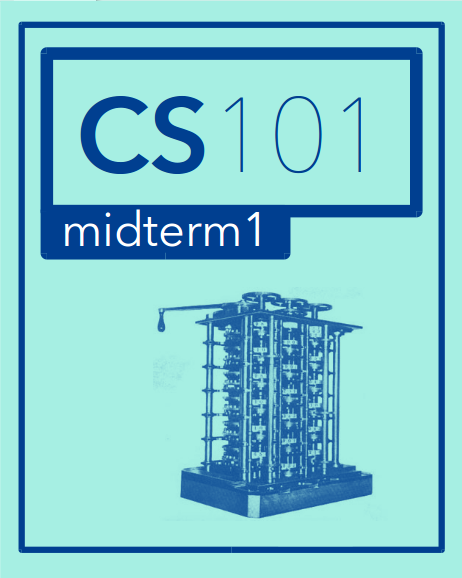
\includegraphics[width=2in]{../img/midterm1-header.png}
\end{center}

\bigskip
\noindent
\begin{itemize}
\item \textbf{Be sure to enter your \underline{NetID} and \underline{the code below} on your Scantron}.
\item Do not turn this page until instructed to do so.
\item There are 30 questions, worth 1 point each.
\item Each question has only \textbf{one} correct answer.
\item You must not communicate with other students during this test.
\item No books, notes, or electronic devices are permitted.
\item This is a 60-minute exam.
\item There are several different versions of this exam.
\end{itemize}

\bigskip\bigskip
\noindent
\textbf{\Large 1. Fill in your information:}

\bigskip
{\Large\bf
\begin{tabular}{ll}
Full Name: & \underbar{\hskip 8cm} \\[0.5em]
UIN (Student Number): & \underbar{\hskip 8cm} \\[0.5em]
NetID: & \underbar{\hskip 8cm}
\end{tabular}
}

\bigskip
\bigskip
\noindent
\textbf{\Large 2. Fill in the following answers on the Scantron form:}

%%%%%%%%%%%%%%%%%%%%%%%%%%%%%%%%%%%%%%%%%%%%%%%%%%%%%%%%%
%%%%%%%%%%%%%%%%%%%%%%%%%%%%%%%%%%%%%%%%%%%%%%%%%%%%%%%%%

\begin{enumerate}
\item[92.] A
\item[93.] E
\item[94.] B
\item[95.] D
\item[96.] D
\end{enumerate}

\newpage

% Zone 1


%%%%%%%%%%%%%%%%%%%%%%%%%%%%%%%%%%%%%%%%%%%%%%%%%%%%%%%%%



\newpage
\noindent
1. (1 point)
Consider the following program.
\begin{verbatim}
kay = 2
wart = 3

def knight(kay,wart):
    wart += 2
    kay += 3
    return wart + kay

wart = knight(kay, kay) + knight(wart, wart)
\end{verbatim}
After it is run, what is the final \textbf{value} of \texttt{wart}?


\begin{enumerate}
\item[(A)] $\bigstar$ 
None of the other answers are correct.

\item[(B)]
\begin{verbatim}2\end{verbatim}

\item[(C)]
\begin{verbatim}3\end{verbatim}

\item[(D)]
\begin{verbatim}5\end{verbatim}

\end{enumerate}

\vspace*{2em}
\hrule
\vspace{2em}

\noindent {\bf Solution.} 
\vspace{2em}
\hrule height 2pt


\newpage
\noindent
2. (1 point)
Consider the following program:
\begin{verbatim}
a=["merlin","sir agravaine","king pellinore"]
b=[ ]
for i in range(0,3):
    b.append(a[0-i].title())
\end{verbatim}
What is the \textbf{value} of b after this program is executed?


\begin{enumerate}
\item[(A)]
\begin{verbatim}[ ]\end{verbatim}

\item[(B)]
\begin{verbatim}['King Pellinore', 'Sir Agravaine']\end{verbatim}

\item[(C)] $\bigstar$ 
\begin{verbatim}['Merlin', 'King Pellinore', 'Sir Agravaine']\end{verbatim}

\item[(D)]
\begin{verbatim}['Sir Agravaine', 'King Pellinore']\end{verbatim}

\item[(E)]
\begin{verbatim}['King Pellinore', 'Sir Agravaine', 'Merlin']\end{verbatim}

\end{enumerate}

\vspace*{2em}
\hrule
\vspace{2em}

\noindent {\bf Solution.} 
\vspace{2em}
\hrule height 2pt


\newpage
\noindent
3. (1 point)
Consider the following incomplete Python program.
\begin{verbatim}
s="".join(["0","1","2","1"])
x=0
for i in range(len(s)-1):
    x+=int(???)
\end{verbatim}
What should replace the three question marks so the resulting value of \texttt{x} is 34?


\begin{enumerate}
\item[(A)]
\begin{verbatim}s[i:i+1]\end{verbatim}

\item[(B)]
\begin{verbatim}s[i:i-1]\end{verbatim}

\item[(C)] $\bigstar$ 
\begin{verbatim}s[i:i+2]\end{verbatim}

\item[(D)]
\begin{verbatim}s[i+1:i+2]\end{verbatim}

\end{enumerate}

\vspace*{2em}
\hrule
\vspace{2em}

\noindent {\bf Solution.} 
\vspace{2em}
\hrule height 2pt


\newpage
\noindent
4. (1 point)
Consider the following program:
\begin{verbatim}
x=0
for i in range(2,7):
    if i%3==0:
        x+=3
    elif i%2==0:
        x+=2
    else:
        x+=1
\end{verbatim}
What is the \textbf{value} of \texttt{x} after this program is executed?


\begin{enumerate}
\item[(A)]
\begin{verbatim}14\end{verbatim}

\item[(B)]
\begin{verbatim}10\end{verbatim}

\item[(C)]
\begin{verbatim}12\end{verbatim}

\item[(D)]
\begin{verbatim}13\end{verbatim}

\item[(E)] $\bigstar$ 
\begin{verbatim}11\end{verbatim}

\end{enumerate}

\vspace*{2em}
\hrule
\vspace{2em}

\noindent {\bf Solution.} 
\vspace{2em}
\hrule height 2pt


\newpage
\noindent
5. (1 point)
Consider the following program:
\begin{verbatim}
x=[1,2,3,4,5,6,7,8,9]
x=x[2:-2]
i=1
while i < 3:
    x[i]+=1
    i+=1
\end{verbatim}
What is the \textbf{value} of \texttt{x} after this program is executed?


\begin{enumerate}
\item[(A)]
\begin{verbatim}[2, 4, 5, 5, 6, 7]\end{verbatim}

\item[(B)]
\begin{verbatim}[3, 5, 6, 6, 7, 8]\end{verbatim}

\item[(C)]
\begin{verbatim}[3, 5, 6, 6]\end{verbatim}

\item[(D)]
\begin{verbatim}[2, 4, 5, 6, 6, 7]\end{verbatim}

\item[(E)] $\bigstar$ 
\begin{verbatim}[3, 5, 6, 6, 7]\end{verbatim}

\end{enumerate}

\vspace*{2em}
\hrule
\vspace{2em}

\noindent {\bf Solution.} 
\vspace{2em}
\hrule height 2pt


\newpage
\noindent
6. (1 point)
Evaluate the following expression:
\begin{verbatim}
[1,2]*len("3")
\end{verbatim}
What value is produced?


\begin{enumerate}
\item[(A)]
\begin{verbatim}[1,2,1]\end{verbatim}

\item[(B)] $\bigstar$ 
\begin{verbatim}[1,2]\end{verbatim}

\item[(C)]
\begin{verbatim}[1,2,1,2,1,2]\end{verbatim}

\item[(D)]
\begin{verbatim}[1,2,3]\end{verbatim}

\end{enumerate}

\vspace*{2em}
\hrule
\vspace{2em}

\noindent {\bf Solution.} 
\vspace{2em}
\hrule height 2pt


\newpage
\noindent
7. (1 point)
Consider the following program:
\begin{verbatim}
def fix(s):
    a=list(s)
    a.sort()
    return ''.join(a)

x=["one","two","eleven","twelve"]
s1=fix(x[0]+x[-1])
s2=fix(x[1]+x[-2])

if s1<s2:
    x.sort()
elif s1>s2:
    x.reverse()
else:
    x.append("six")
\end{verbatim}
What is the \textbf{value} of \texttt{x} after this program is executed?


\begin{enumerate}
\item[(A)] $\bigstar$ 
\begin{verbatim}['one', 'two', 'eleven', 'twelve', 'six']\end{verbatim}

\item[(B)]
\begin{verbatim}['one', 'two', 'eleven', 'twelve']\end{verbatim}

\item[(C)]
\begin{verbatim}['twelve', 'eleven', 'two', 'one']\end{verbatim}

\item[(D)]
\begin{verbatim}['two', 'twelve', 'one', 'eleven', 'six']\end{verbatim}

\item[(E)]
\begin{verbatim}['eleven', 'one', 'twelve', 'two']\end{verbatim}

\end{enumerate}

\vspace*{2em}
\hrule
\vspace{2em}

\noindent {\bf Solution.} 
\vspace{2em}
\hrule height 2pt


\newpage
\noindent
8. (1 point)
Consider the following program:
\begin{verbatim}
i=3
x=2
while i < 7:
    x+=i
    i+=2
\end{verbatim}
What is the \textbf{value} of \texttt{x} after this program is executed?


\begin{enumerate}
\item[(A)]
\begin{verbatim}12\end{verbatim}

\item[(B)]
\begin{verbatim}13\end{verbatim}

\item[(C)]
\begin{verbatim}11\end{verbatim}

\item[(D)] $\bigstar$ 
\begin{verbatim}10\end{verbatim}

\item[(E)]
\begin{verbatim}14\end{verbatim}

\end{enumerate}

\vspace*{2em}
\hrule
\vspace{2em}

\noindent {\bf Solution.} 
\vspace{2em}
\hrule height 2pt


\newpage
\noindent
9. (1 point)
Consider the following program:
\begin{verbatim}
s="ECTOR"
t="GAWAIN"
x=(len(s)/(len(t)-1))+1
\end{verbatim}
What is the \textbf{type} of \texttt{x} after this program is executed?


\begin{enumerate}
\item[(A)]
\begin{verbatim}Integer\end{verbatim}

\item[(B)]
\begin{verbatim}None\end{verbatim}

\item[(C)] $\bigstar$ 
\begin{verbatim}Float\end{verbatim}

\item[(D)]
\begin{verbatim}Boolean\end{verbatim}

\item[(E)]
\begin{verbatim}String\end{verbatim}

\end{enumerate}

\vspace*{2em}
\hrule
\vspace{2em}

\noindent {\bf Solution.} 
\vspace{2em}
\hrule height 2pt


\newpage
\noindent
10. (1 point)
How can the following mathematical equation be implemented as a Python expression? Assume \verb|a|, \verb|b|, and \verb|cos| have already been defined.
$$a^b \cos(a - b)$$


\begin{enumerate}
\item[(A)] $\bigstar$ 
\begin{verbatim}(a**b)*cos(a-b)\end{verbatim}

\item[(B)]
\begin{verbatim}(a^b)*cos(a-b)\end{verbatim}

\item[(C)]
None of the other answers are correct.

\item[(D)]
\begin{verbatim}(a**b)cos(a-b)\end{verbatim}

\item[(E)]
\begin{verbatim}(b^a)cos(a-b)\end{verbatim}

\end{enumerate}

\vspace*{2em}
\hrule
\vspace{2em}

\noindent {\bf Solution.} 
\vspace{2em}
\hrule height 2pt


\newpage
\noindent
11. (1 point)
Consider the following program:
\begin{verbatim}
a=3
b=4
if a==3:
    a=b
elif a==4:
    a=5
else:
    b=a
\end{verbatim}
What is the \textbf{value} of a after this program is executed?


\begin{enumerate}
\item[(A)]
\begin{verbatim}5\end{verbatim}

\item[(B)] $\bigstar$ 
\begin{verbatim}4\end{verbatim}

\item[(C)]
\begin{verbatim}3\end{verbatim}

\item[(D)]
\begin{verbatim}7\end{verbatim}

\item[(E)]
None of the other answers are correct.

\end{enumerate}

\vspace*{2em}
\hrule
\vspace{2em}

\noindent {\bf Solution.} 
\vspace{2em}
\hrule height 2pt


\newpage
\noindent
12. (1 point)
For this problem, you should compose a function which accomplishes a given task using the available code blocks arranged in the correct functional order.  \emph{We ignore indentation for this problem.}

\texttt{find\_max} should accept a \texttt{list} and return the value of the maximum item in the \texttt{list}.  (\texttt{None} is always the lowest value in any numeric comparison, so you may use it as an initializer.)

\begin{verbatim}
def find_max(my_list):
\end{verbatim}

\begin{enumerate}[1]
\item \texttt{max\_val = i}
\item \texttt{max\_val = None}
\item \texttt{for i in range(len(my\_list)):}
\item \texttt{if i > max\_val:}
\item \texttt{max\_val = my\_list[i]}
\item \texttt{return max\_val}
\item \texttt{for i in range(my\_list):}
\item \texttt{if my\_list[i] > max\_val:}
\item \texttt{print(max\_val)}
\end{enumerate}



\begin{enumerate}
\item[(A)]
3, 2, 8, 5, 9

\item[(B)] $\bigstar$ 
2, 3, 8, 5, 6

\item[(C)]
2, 3, 4, 1, 6

\item[(D)]
2, 3, 8, 1, 6

\item[(E)]
2, 7, 4, 5, 6

\end{enumerate}

\vspace*{2em}
\hrule
\vspace{2em}

\noindent {\bf Solution.} 
\vspace{2em}
\hrule height 2pt


\newpage
\noindent
13. (1 point)
Consider the following program:
\begin{verbatim}
a=["A","C","C","I","O"]
a.sort()
a[0]=a[-1]
x=""
for e in a:
    x=x+e
\end{verbatim}
What is the \textbf{value} of \texttt{x} after this program is executed?


\begin{enumerate}
\item[(A)]
None of the other answers are correct.

\item[(B)] $\bigstar$ 
\begin{verbatim}"OCCIO"\end{verbatim}

\item[(C)]
\begin{verbatim}"ACCOA"\end{verbatim}

\item[(D)]
\begin{verbatim}"ICCOI"\end{verbatim}

\item[(E)]
\begin{verbatim}"ACCIA"\end{verbatim}

\end{enumerate}

\vspace*{2em}
\hrule
\vspace{2em}

\noindent {\bf Solution.} 
\vspace{2em}
\hrule height 2pt


\newpage
\noindent
14. (1 point)
Consider the following program:
\begin{verbatim}
s="-B-O-R-S-"
x=s.split("-")[2:-2]
\end{verbatim}
What is the \textbf{value} of \texttt{x} after this program is executed?


\begin{enumerate}
\item[(A)]
\begin{verbatim}'ORS'\end{verbatim}

\item[(B)]
\begin{verbatim}''\end{verbatim}

\item[(C)]
\begin{verbatim}False\end{verbatim}

\item[(D)]
\begin{verbatim}None\end{verbatim}

\item[(E)] $\bigstar$ 
\begin{verbatim}['O', 'R']\end{verbatim}

\end{enumerate}

\vspace*{2em}
\hrule
\vspace{2em}

\noindent {\bf Solution.} 
\vspace{2em}
\hrule height 2pt


\newpage
\noindent
15. (1 point)
Consider the following program:
\begin{verbatim}
x=3
a=7
if (a%3)==2:
    x=x**2
elif(a%3)==1:
    x=x**1
else:
    x=x**0
\end{verbatim}
What is the \textbf{value} of \texttt{x} after this program is executed?


\begin{enumerate}
\item[(A)] $\bigstar$ 
\begin{verbatim}3\end{verbatim}

\item[(B)]
\begin{verbatim}9\end{verbatim}

\item[(C)]
None of the other answers are correct.

\item[(D)]
\begin{verbatim}1\end{verbatim}

\item[(E)]
\begin{verbatim}7\end{verbatim}

\end{enumerate}

\vspace*{2em}
\hrule
\vspace{2em}

\noindent {\bf Solution.} 
\vspace{2em}
\hrule height 2pt


\newpage
\noindent
16. (1 point)
Consider the following program:
\begin{verbatim}
x=str("1"*3)
\end{verbatim}
What is the \textbf{value} of \texttt{x} after this program is executed?


\begin{enumerate}
\item[(A)] $\bigstar$ 
\begin{verbatim}"111"\end{verbatim}

\item[(B)]
None of the other answers are correct.

\item[(C)]
\begin{verbatim}"3"\end{verbatim}

\item[(D)]
\begin{verbatim}111\end{verbatim}

\item[(E)]
\begin{verbatim}3\end{verbatim}

\end{enumerate}

\vspace*{2em}
\hrule
\vspace{2em}

\noindent {\bf Solution.} 
\vspace{2em}
\hrule height 2pt


\newpage
\noindent
17. (1 point)
What is the result of the following expression?
\begin{verbatim}
[ 1, 2, 3 ] * 3.0
\end{verbatim}


\begin{enumerate}
\item[(A)] $\bigstar$ 
\begin{verbatim}[1, 2, 3, 1, 2, 3, 1, 2, 3]\end{verbatim}

\item[(B)]
\begin{verbatim}[3, 6, 9]\end{verbatim}

\item[(C)]
\begin{verbatim}[3.0, 6.0, 9.0]\end{verbatim}

\item[(D)]
\begin{verbatim}[1.0, 2.0, 3.0, 1.0, 2.0, 3.0, 1.0, 2.0, 3.0]\end{verbatim}

\item[(E)]
\begin{verbatim}None of the above.\end{verbatim}

\end{enumerate}

\vspace*{2em}
\hrule
\vspace{2em}

\noindent {\bf Solution.} 
\vspace{2em}
\hrule height 2pt


\newpage
\noindent
18. (1 point)
Consider the following program.
\begin{verbatim}
x=[]
for j in range(0,5):
    if (j%3)==0:
        x.append("-")
    if (j%4)==0:
        x.append("*")
\end{verbatim}
After it is run, what is the final \textbf{value} of \texttt{x}?


\begin{enumerate}
\item[(A)]
\begin{verbatim}["*","-","*"]\end{verbatim}

\item[(B)] $\bigstar$ 
\begin{verbatim}["-","*","-","*"]\end{verbatim}

\item[(C)]
\begin{verbatim}["-","*"]\end{verbatim}

\item[(D)]
\begin{verbatim}["*","-","*"]\end{verbatim}

\item[(E)]
None of the other answers are correct.

\end{enumerate}

\vspace*{2em}
\hrule
\vspace{2em}

\noindent {\bf Solution.} 
\vspace{2em}
\hrule height 2pt


\newpage
\noindent
19. (1 point)
Consider the following program.
\begin{verbatim}
x=0
i=1
while(i*i)<=9:
    x=x+(i*i)
    i=i+1
\end{verbatim}
After it is run, what is the final \textbf{value} of \texttt{x}?


\begin{enumerate}
\item[(A)]
\begin{verbatim}5\end{verbatim}

\item[(B)]
\begin{verbatim}30\end{verbatim}

\item[(C)]
\begin{verbatim}4\end{verbatim}

\item[(D)] $\bigstar$ 
\begin{verbatim}14\end{verbatim}

\item[(E)]
\begin{verbatim}3\end{verbatim}

\end{enumerate}

\vspace*{2em}
\hrule
\vspace{2em}

\noindent {\bf Solution.} 
\vspace{2em}
\hrule height 2pt


\newpage
\noindent
20. (1 point)
Evaluate the following expression:
\begin{verbatim}
len("ABCDE"[1:4])
\end{verbatim}
What value is produced?


\begin{enumerate}
\item[(A)]
1

\item[(B)]
5

\item[(C)] $\bigstar$ 
3

\item[(D)]
4

\end{enumerate}

\vspace*{2em}
\hrule
\vspace{2em}

\noindent {\bf Solution.} 
\vspace{2em}
\hrule height 2pt


\newpage
\noindent
21. (1 point)
Consider the following incomplete function.
\begin{verbatim}
def isdivisible(m,n):
    if ???:
        return False
    else:
        return True
\end{verbatim}
The function is intended to return True if the input parameter m is evenly divisible by the parameter n and False otherwise. For example, \verb|isdivisible(4,2)| should return \verb|True|, but \verb|isdivisible(5,3)| should return \verb|False|. What should replace the three question marks to complete the function?


\begin{enumerate}
\item[(A)]
\begin{verbatim}(n % m) == 0 \end{verbatim}

\item[(B)]
\begin{verbatim}(n // m) == 0 \end{verbatim}

\item[(C)]
\begin{verbatim}(m // n) != 0 \end{verbatim}

\item[(D)] $\bigstar$ 
\begin{verbatim}(m % n) != 0 \end{verbatim}

\end{enumerate}

\vspace*{2em}
\hrule
\vspace{2em}

\noindent {\bf Solution.} 
\vspace{2em}
\hrule height 2pt


\newpage
\noindent
22. (1 point)
Consider the following program:
\begin{verbatim}
pi="3.14159"
e="2.71828"
x=(float(e)**float(pi)-float(pi)) == 20
\end{verbatim}
What is the \textbf{type} of \texttt{x} after this program is executed?


\begin{enumerate}
\item[(A)]
\begin{verbatim}None\end{verbatim}

\item[(B)]
\begin{verbatim}Integer\end{verbatim}

\item[(C)]
\begin{verbatim}String\end{verbatim}

\item[(D)] $\bigstar$ 
\begin{verbatim}Boolean\end{verbatim}

\item[(E)]
\begin{verbatim}Float\end{verbatim}

\end{enumerate}

\vspace*{2em}
\hrule
\vspace{2em}

\noindent {\bf Solution.} 
\vspace{2em}
\hrule height 2pt


\newpage
\noindent
23. (1 point)
Consider the following program:
\begin{verbatim}
x=[1,2,3]
def f(a):
    s=""
    a.append(4)
    for i in a:
        s+=str(i)
    return s

x.append(f(x))
\end{verbatim}
What is the \textbf{value} of \texttt{x} after this program is executed?


\begin{enumerate}
\item[(A)]
\begin{verbatim}[1, 2, 3, '123']\end{verbatim}

\item[(B)]
\begin{verbatim}[1, 2, 3, 10]\end{verbatim}

\item[(C)] $\bigstar$ 
\begin{verbatim}[1, 2, 3, 4, '1234']\end{verbatim}

\item[(D)]
\begin{verbatim}[1, 2, 3]\end{verbatim}

\item[(E)]
\begin{verbatim}[1, 2, 3, '1234']\end{verbatim}

\end{enumerate}

\vspace*{2em}
\hrule
\vspace{2em}

\noindent {\bf Solution.} 
\vspace{2em}
\hrule height 2pt


\newpage
\noindent
24. (1 point)
Consider the following program:
\begin{verbatim}
s="Hobbes"
i=0
x=-1
while i<len(s):
    if s[i]=='b':
        x=i
    i+=1
\end{verbatim}
What is the \textbf{value} of \texttt{x} after this program is executed?


\begin{enumerate}
\item[(A)]
\begin{verbatim}-1\end{verbatim}

\item[(B)] $\bigstar$ 
\begin{verbatim}3\end{verbatim}

\item[(C)]
\begin{verbatim}4\end{verbatim}

\item[(D)]
\begin{verbatim}2\end{verbatim}

\item[(E)]
\begin{verbatim}5\end{verbatim}

\end{enumerate}

\vspace*{2em}
\hrule
\vspace{2em}

\noindent {\bf Solution.} 
\vspace{2em}
\hrule height 2pt


\newpage
\noindent
25. (1 point)
Consider the following Python program.
\begin{verbatim}
e=[1,3,5,7,9,11]
d=[0,0,0]
for i in range(0,len(e)):
    d[i%3]+=e[i]
x=d[2]
\end{verbatim}
After it is run, what is the final \textbf{value} of \texttt{x}?


\begin{enumerate}
\item[(A)]
\begin{verbatim}12\end{verbatim}

\item[(B)]
\begin{verbatim}8\end{verbatim}

\item[(C)]
\begin{verbatim}0\end{verbatim}

\item[(D)]
\begin{verbatim}7\end{verbatim}

\item[(E)] $\bigstar$ 
\begin{verbatim}16\end{verbatim}

\end{enumerate}

\vspace*{2em}
\hrule
\vspace{2em}

\noindent {\bf Solution.} 
\vspace{2em}
\hrule height 2pt


\newpage
\noindent
26. (1 point)
Consider the following program.
\begin{verbatim}
s="BBCAA"
x=0
y=len(s)-1
while s[x]!=s[y] and x<len(s):
    x+=1
    y-=1
\end{verbatim}
After it is run, what is the final \textbf{value} of \texttt{x}?


\begin{enumerate}
\item[(A)]
\begin{verbatim}3\end{verbatim}

\item[(B)]
\begin{verbatim}0\end{verbatim}

\item[(C)]
\begin{verbatim}4\end{verbatim}

\item[(D)] $\bigstar$ 
\begin{verbatim}2\end{verbatim}

\item[(E)]
\begin{verbatim}1\end{verbatim}

\end{enumerate}

\vspace*{2em}
\hrule
\vspace{2em}

\noindent {\bf Solution.} 
\vspace{2em}
\hrule height 2pt


\newpage
\noindent
27. (1 point)
Consider the following program:
\begin{verbatim}
x="KING ARTHUR-MORGANA LEFAY-SIR BEDIVERE".split("-")
y=x
y.reverse()
\end{verbatim}
What is the \textbf{value} of \texttt{x} after this program is executed?


\begin{enumerate}
\item[(A)] $\bigstar$ 
\begin{verbatim}['SIR BEDIVERE', 'MORGANA LEFAY', 'KING ARTHUR']\end{verbatim}

\item[(B)]
\begin{verbatim}['KING', 'ARTHUR-MORGANA', 'LEFAY-SIR', 'BEDIVERE']\end{verbatim}

\item[(C)]
\begin{verbatim}None\end{verbatim}

\item[(D)]
\begin{verbatim}['BEDIVERE', 'LEFAY-SIR', 'ARTHUR-MORGANA', 'KING']\end{verbatim}

\item[(E)]
\begin{verbatim}['KING ARTHUR', 'MORGANA LEFAY', 'SIR BEDIVERE']\end{verbatim}

\end{enumerate}

\vspace*{2em}
\hrule
\vspace{2em}

\noindent {\bf Solution.} 
\vspace{2em}
\hrule height 2pt


\newpage
\noindent
28. (1 point)
Consider the following program.
\begin{verbatim}
def artificing(s):
    return s+"%i" % 2
    return s*2
    return s

s=artificing("MERLIN")
\end{verbatim}
After it is run, what is the final \textbf{value} of s?


\begin{enumerate}
\item[(A)]
\begin{verbatim}0\end{verbatim}

\item[(B)] $\bigstar$ 
\begin{verbatim}"MERLIN2"\end{verbatim}

\item[(C)]
\begin{verbatim}None\end{verbatim}

\item[(D)]
\begin{verbatim}"MERLINMERLIN"\end{verbatim}

\item[(E)]
\begin{verbatim}"MERLIN%i"\end{verbatim}

\end{enumerate}

\vspace*{2em}
\hrule
\vspace{2em}

\noindent {\bf Solution.} 
\vspace{2em}
\hrule height 2pt


\newpage
\noindent
29. (1 point)
Consider the following incomplete program.
\begin{verbatim}
sum=0
???:
    sum=sum+i

\end{verbatim}
The program is intended to sum all of the integers between 1 and 100 (inclusive). What should replace the three question marks to complete the program?


\begin{enumerate}
\item[(A)]
\begin{verbatim}while i in range(100)\end{verbatim}

\item[(B)]
\begin{verbatim}for i in range(0,100)\end{verbatim}

\item[(C)] $\bigstar$ 
\begin{verbatim}for i in range(1,101) \end{verbatim}

\item[(D)]
\begin{verbatim}while i<=100 \end{verbatim}

\end{enumerate}

\vspace*{2em}
\hrule
\vspace{2em}

\noindent {\bf Solution.} 
\vspace{2em}
\hrule height 2pt


\newpage
\noindent
30. (1 point)
Consider the following program:
\begin{verbatim}
s="TRIS %i"
t="ISEU"
x=s % len(t)
\end{verbatim}
What is the \textbf{type} of \texttt{x} after this program is executed?


\begin{enumerate}
\item[(A)]
\begin{verbatim}None\end{verbatim}

\item[(B)]
\begin{verbatim}Float\end{verbatim}

\item[(C)]
\begin{verbatim}Boolean\end{verbatim}

\item[(D)] $\bigstar$ 
\begin{verbatim}String\end{verbatim}

\item[(E)]
\begin{verbatim}Integer\end{verbatim}

\end{enumerate}

\vspace*{2em}
\hrule
\vspace{2em}

\noindent {\bf Solution.} 
\vspace{2em}
\hrule height 2pt

%%%%%%%%%%%%%%%%%%%%%%%%%%%%%%%%%%%%%%%%%%%%%%%%%%%%%%%%%%%%%%%%%%%%%%
%%%%%%%%%%%%%%%%%%%%%%%%%%%%%%%%%%%%%%%%%%%%%%%%%%%%%%%%%%%%%%%%%%%%%%
%%%%%%%%%%%%%%%%%%%%%%%%%%%%%%%%%%%%%%%%%%%%%%%%%%%%%%%%%%%%%%%%%%%%%%
%%%%%%%%%%%%%%%%%%%%%%%%%%%%%%%%%%%%%%%%%%%%%%%%%%%%%%%%%%%%%%%%%%%%%%
% Exam number 47

\message{Exam 47/50}
\cleardoublepage
\setcounter{page}{1}


\begin{center}
%\textbf{\Large CS 101 Midterm \#1}
%
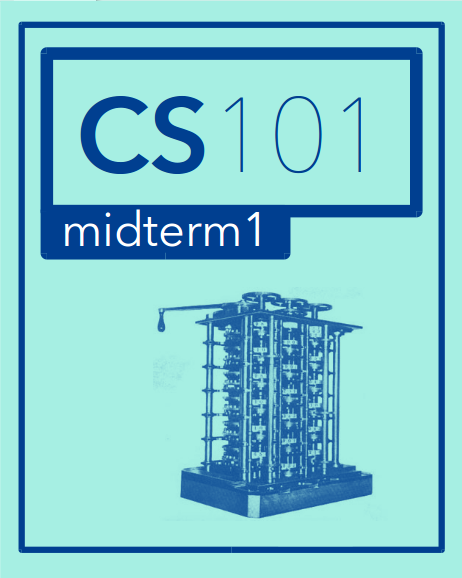
\includegraphics[width=2in]{../img/midterm1-header.png}
\end{center}

\bigskip
\noindent
\begin{itemize}
\item \textbf{Be sure to enter your \underline{NetID} and \underline{the code below} on your Scantron}.
\item Do not turn this page until instructed to do so.
\item There are 30 questions, worth 1 point each.
\item Each question has only \textbf{one} correct answer.
\item You must not communicate with other students during this test.
\item No books, notes, or electronic devices are permitted.
\item This is a 60-minute exam.
\item There are several different versions of this exam.
\end{itemize}

\bigskip\bigskip
\noindent
\textbf{\Large 1. Fill in your information:}

\bigskip
{\Large\bf
\begin{tabular}{ll}
Full Name: & \underbar{\hskip 8cm} \\[0.5em]
UIN (Student Number): & \underbar{\hskip 8cm} \\[0.5em]
NetID: & \underbar{\hskip 8cm}
\end{tabular}
}

\bigskip
\bigskip
\noindent
\textbf{\Large 2. Fill in the following answers on the Scantron form:}

%%%%%%%%%%%%%%%%%%%%%%%%%%%%%%%%%%%%%%%%%%%%%%%%%%%%%%%%%
%%%%%%%%%%%%%%%%%%%%%%%%%%%%%%%%%%%%%%%%%%%%%%%%%%%%%%%%%

\begin{enumerate}
\item[92.] B
\item[93.] E
\item[94.] B
\item[95.] E
\item[96.] E
\end{enumerate}

\newpage

% Zone 1


%%%%%%%%%%%%%%%%%%%%%%%%%%%%%%%%%%%%%%%%%%%%%%%%%%%%%%%%%



\newpage
\noindent
1. (1 point)
What is the result of the following expression?
\begin{verbatim}
[ 1, 2, 3 ] * 3.0
\end{verbatim}


\begin{enumerate}
\item[(A)]
\begin{verbatim}[3, 6, 9]\end{verbatim}

\item[(B)]
\begin{verbatim}None of the above.\end{verbatim}

\item[(C)]
\begin{verbatim}[3.0, 6.0, 9.0]\end{verbatim}

\item[(D)] $\bigstar$ 
\begin{verbatim}[1, 2, 3, 1, 2, 3, 1, 2, 3]\end{verbatim}

\item[(E)]
\begin{verbatim}[1.0, 2.0, 3.0, 1.0, 2.0, 3.0, 1.0, 2.0, 3.0]\end{verbatim}

\end{enumerate}

\vspace*{2em}
\hrule
\vspace{2em}

\noindent {\bf Solution.} 
\vspace{2em}
\hrule height 2pt


\newpage
\noindent
2. (1 point)
Consider the following program:
\begin{verbatim}
a=3
b=4
if a==3:
    a=b
elif a==4:
    a=5
else:
    b=a
\end{verbatim}
What is the \textbf{value} of a after this program is executed?


\begin{enumerate}
\item[(A)]
\begin{verbatim}3\end{verbatim}

\item[(B)] $\bigstar$ 
\begin{verbatim}4\end{verbatim}

\item[(C)]
None of the other answers are correct.

\item[(D)]
\begin{verbatim}7\end{verbatim}

\item[(E)]
\begin{verbatim}5\end{verbatim}

\end{enumerate}

\vspace*{2em}
\hrule
\vspace{2em}

\noindent {\bf Solution.} 
\vspace{2em}
\hrule height 2pt


\newpage
\noindent
3. (1 point)
Evaluate the following expression:
\begin{verbatim}
len("ABCD"[0:3])
\end{verbatim}
What value is produced?


\begin{enumerate}
\item[(A)] $\bigstar$ 
3

\item[(B)]
2

\item[(C)]
1

\item[(D)]
4

\end{enumerate}

\vspace*{2em}
\hrule
\vspace{2em}

\noindent {\bf Solution.} 
\vspace{2em}
\hrule height 2pt


\newpage
\noindent
4. (1 point)
Consider the following program:
\begin{verbatim}
def fix(s):
    a=list(s)
    a.sort()
    return ''.join(a)

x=["one","two","eleven","twelve"]
s1=fix(x[0]+x[-1])
s2=fix(x[1]+x[-2])

if s1<s2:
    x.sort()
elif s1>s2:
    x.reverse()
else:
    x.append("six")
\end{verbatim}
What is the \textbf{value} of \texttt{x} after this program is executed?


\begin{enumerate}
\item[(A)]
\begin{verbatim}['twelve', 'eleven', 'two', 'one']\end{verbatim}

\item[(B)] $\bigstar$ 
\begin{verbatim}['one', 'two', 'eleven', 'twelve', 'six']\end{verbatim}

\item[(C)]
\begin{verbatim}['two', 'twelve', 'one', 'eleven', 'six']\end{verbatim}

\item[(D)]
\begin{verbatim}['one', 'two', 'eleven', 'twelve']\end{verbatim}

\item[(E)]
\begin{verbatim}['eleven', 'one', 'twelve', 'two']\end{verbatim}

\end{enumerate}

\vspace*{2em}
\hrule
\vspace{2em}

\noindent {\bf Solution.} 
\vspace{2em}
\hrule height 2pt


\newpage
\noindent
5. (1 point)
Consider the following incomplete Python program.
\begin{verbatim}
s="".join(["0","1","2","1"])
x=0
for i in range(len(s)-1):
    x+=int(???)
\end{verbatim}
What should replace the three question marks so the resulting value of \texttt{x} is 34?


\begin{enumerate}
\item[(A)] $\bigstar$ 
\begin{verbatim}s[i:i+2]\end{verbatim}

\item[(B)]
\begin{verbatim}s[i:i+1]\end{verbatim}

\item[(C)]
\begin{verbatim}s[i+1:i+2]\end{verbatim}

\item[(D)]
\begin{verbatim}s[i:i-1]\end{verbatim}

\end{enumerate}

\vspace*{2em}
\hrule
\vspace{2em}

\noindent {\bf Solution.} 
\vspace{2em}
\hrule height 2pt


\newpage
\noindent
6. (1 point)
Consider the following program:
\begin{verbatim}
s="ECTOR"
t="GAWAIN"
x=len(str(s.isupper()))-t.find("A")
\end{verbatim}
What is the \textbf{type} of \texttt{x} after this program is executed?


\begin{enumerate}
\item[(A)]
\begin{verbatim}None\end{verbatim}

\item[(B)]
\begin{verbatim}Boolean\end{verbatim}

\item[(C)]
\begin{verbatim}Float\end{verbatim}

\item[(D)] $\bigstar$ 
\begin{verbatim}Integer\end{verbatim}

\item[(E)]
\begin{verbatim}String\end{verbatim}

\end{enumerate}

\vspace*{2em}
\hrule
\vspace{2em}

\noindent {\bf Solution.} 
\vspace{2em}
\hrule height 2pt


\newpage
\noindent
7. (1 point)
Consider the following program:
\begin{verbatim}
s="Hobbes"
i=0
x=-1
while i<len(s):
    if s[i]=='b':
        x=i
    i+=1
\end{verbatim}
What is the \textbf{value} of \texttt{x} after this program is executed?


\begin{enumerate}
\item[(A)]
\begin{verbatim}4\end{verbatim}

\item[(B)] $\bigstar$ 
\begin{verbatim}3\end{verbatim}

\item[(C)]
\begin{verbatim}-1\end{verbatim}

\item[(D)]
\begin{verbatim}2\end{verbatim}

\item[(E)]
\begin{verbatim}5\end{verbatim}

\end{enumerate}

\vspace*{2em}
\hrule
\vspace{2em}

\noindent {\bf Solution.} 
\vspace{2em}
\hrule height 2pt


\newpage
\noindent
8. (1 point)
Consider the following program:
\begin{verbatim}
i=3
x=2
while i < 7:
    x+=i
    i+=2
\end{verbatim}
What is the \textbf{value} of \texttt{x} after this program is executed?


\begin{enumerate}
\item[(A)]
\begin{verbatim}14\end{verbatim}

\item[(B)]
\begin{verbatim}11\end{verbatim}

\item[(C)]
\begin{verbatim}13\end{verbatim}

\item[(D)] $\bigstar$ 
\begin{verbatim}10\end{verbatim}

\item[(E)]
\begin{verbatim}12\end{verbatim}

\end{enumerate}

\vspace*{2em}
\hrule
\vspace{2em}

\noindent {\bf Solution.} 
\vspace{2em}
\hrule height 2pt


\newpage
\noindent
9. (1 point)
Evaluate the following expression:
\begin{verbatim}
[1,2]*len("3")
\end{verbatim}
What value is produced?


\begin{enumerate}
\item[(A)] $\bigstar$ 
\begin{verbatim}[1,2]\end{verbatim}

\item[(B)]
\begin{verbatim}[1,2,1,2,1,2]\end{verbatim}

\item[(C)]
\begin{verbatim}[1,2,3]\end{verbatim}

\item[(D)]
\begin{verbatim}[1,2,1]\end{verbatim}

\end{enumerate}

\vspace*{2em}
\hrule
\vspace{2em}

\noindent {\bf Solution.} 
\vspace{2em}
\hrule height 2pt


\newpage
\noindent
10. (1 point)
Consider the following program:
\begin{verbatim}
x=[1,2,3,4,5,6,7,8,9]
x=x[2:-2]
i=1
while i <= 3:
    x[i]+=1
    i+=1
\end{verbatim}
What is the \textbf{value} of \texttt{x} after this program is executed?


\begin{enumerate}
\item[(A)]
\begin{verbatim}[3, 5, 7, 7]\end{verbatim}

\item[(B)] $\bigstar$ 
\begin{verbatim}[3, 5, 6, 7, 7]\end{verbatim}

\item[(C)]
\begin{verbatim}[2, 4, 5, 6, 7, 7]\end{verbatim}

\item[(D)]
\begin{verbatim}[2, 4, 5, 5, 7, 7]\end{verbatim}

\item[(E)]
\begin{verbatim}[3, 5, 6, 7, 7, 8]\end{verbatim}

\end{enumerate}

\vspace*{2em}
\hrule
\vspace{2em}

\noindent {\bf Solution.} 
\vspace{2em}
\hrule height 2pt


\newpage
\noindent
11. (1 point)
Consider the following program.
\begin{verbatim}
def artificing(s):
    return s+"%i" % 2
    return s*2
    return s

s=artificing("MERLIN")
\end{verbatim}
After it is run, what is the final \textbf{value} of s?


\begin{enumerate}
\item[(A)]
\begin{verbatim}None\end{verbatim}

\item[(B)] $\bigstar$ 
\begin{verbatim}"MERLIN2"\end{verbatim}

\item[(C)]
\begin{verbatim}"MERLIN%i"\end{verbatim}

\item[(D)]
\begin{verbatim}0\end{verbatim}

\item[(E)]
\begin{verbatim}"MERLINMERLIN"\end{verbatim}

\end{enumerate}

\vspace*{2em}
\hrule
\vspace{2em}

\noindent {\bf Solution.} 
\vspace{2em}
\hrule height 2pt


\newpage
\noindent
12. (1 point)
Consider the following incomplete program.
\begin{verbatim}
sum=0
???:
    sum=sum+i

\end{verbatim}
The program is intended to sum all of the integers between 1 and 100 (inclusive). What should replace the three question marks to complete the program?


\begin{enumerate}
\item[(A)] $\bigstar$ 
\begin{verbatim}for i in range(1,101) \end{verbatim}

\item[(B)]
\begin{verbatim}for i in range(0,100)\end{verbatim}

\item[(C)]
\begin{verbatim}while i<=100 \end{verbatim}

\item[(D)]
\begin{verbatim}while i in range(100)\end{verbatim}

\end{enumerate}

\vspace*{2em}
\hrule
\vspace{2em}

\noindent {\bf Solution.} 
\vspace{2em}
\hrule height 2pt


\newpage
\noindent
13. (1 point)
Consider the following incomplete function.
\begin{verbatim}
def ismultiple(m,n):
    if ???:
        return False
    else:
        return True
\end{verbatim}
The function is intended to return True if the input parameter m is a multiple of parameter n and False otherwise. For example, \verb|ismultiple(4,2)| should return \verb|True|, but \verb|ismultiple(5,3)| should return \verb|False|. What should replace the three question marks to complete the function?


\begin{enumerate}
\item[(A)]
\begin{verbatim}(n % m) == 0 \end{verbatim}

\item[(B)]
\begin{verbatim}(m // n) != 0 \end{verbatim}

\item[(C)] $\bigstar$ 
\begin{verbatim}(m % n) != 0 \end{verbatim}

\item[(D)]
\begin{verbatim}(n // m) == 0 \end{verbatim}

\end{enumerate}

\vspace*{2em}
\hrule
\vspace{2em}

\noindent {\bf Solution.} 
\vspace{2em}
\hrule height 2pt


\newpage
\noindent
14. (1 point)
Consider the following program.
\begin{verbatim}
x=[]
for j in range(0,5):
    if (j%3)==0:
        x.append("-")
    if (j%4)==0:
        x.append("*")
\end{verbatim}
After it is run, what is the final \textbf{value} of \texttt{x}?


\begin{enumerate}
\item[(A)]
\begin{verbatim}["*","-","*"]\end{verbatim}

\item[(B)]
\begin{verbatim}["*","-","*"]\end{verbatim}

\item[(C)]
None of the other answers are correct.

\item[(D)]
\begin{verbatim}["-","*"]\end{verbatim}

\item[(E)] $\bigstar$ 
\begin{verbatim}["-","*","-","*"]\end{verbatim}

\end{enumerate}

\vspace*{2em}
\hrule
\vspace{2em}

\noindent {\bf Solution.} 
\vspace{2em}
\hrule height 2pt


\newpage
\noindent
15. (1 point)
Consider the following program:
\begin{verbatim}
s="TRIS %i"
t="ISEU"
x=s % len(t)
\end{verbatim}
What is the \textbf{type} of \texttt{x} after this program is executed?


\begin{enumerate}
\item[(A)]
\begin{verbatim}None\end{verbatim}

\item[(B)]
\begin{verbatim}Boolean\end{verbatim}

\item[(C)]
\begin{verbatim}Float\end{verbatim}

\item[(D)]
\begin{verbatim}Integer\end{verbatim}

\item[(E)] $\bigstar$ 
\begin{verbatim}String\end{verbatim}

\end{enumerate}

\vspace*{2em}
\hrule
\vspace{2em}

\noindent {\bf Solution.} 
\vspace{2em}
\hrule height 2pt


\newpage
\noindent
16. (1 point)
Consider the following Python program.
\begin{verbatim}
e=[1,3,5,7,9,11]
d=[0,0,0]
for i in range(0,len(e)):
    d[i%3]+=e[i]
x=d[1]
\end{verbatim}
After it is run, what is the final \textbf{value} of \texttt{x}?


\begin{enumerate}
\item[(A)]
\begin{verbatim}3\end{verbatim}

\item[(B)]
\begin{verbatim}16\end{verbatim}

\item[(C)]
\begin{verbatim}8\end{verbatim}

\item[(D)]
\begin{verbatim}0\end{verbatim}

\item[(E)] $\bigstar$ 
\begin{verbatim}12\end{verbatim}

\end{enumerate}

\vspace*{2em}
\hrule
\vspace{2em}

\noindent {\bf Solution.} 
\vspace{2em}
\hrule height 2pt


\newpage
\noindent
17. (1 point)
How can the following mathematical equation be implemented as a Python expression? Assume \verb|a|, \verb|b|, and \verb|sin| have already been defined.
$$a \sin(a^b - b)$$


\begin{enumerate}
\item[(A)] $\bigstar$ 
\begin{verbatim}a*sin(a**b - b)\end{verbatim}

\item[(B)]
\begin{verbatim}a sin(a**b - b)\end{verbatim}

\item[(C)]
\begin{verbatim}a*sin(b^a - b)\end{verbatim}

\item[(D)]
\begin{verbatim}a*sin(a^b - b)\end{verbatim}

\item[(E)]
None of the other answers are correct.

\end{enumerate}

\vspace*{2em}
\hrule
\vspace{2em}

\noindent {\bf Solution.} 
\vspace{2em}
\hrule height 2pt


\newpage
\noindent
18. (1 point)
Consider the following program:
\begin{verbatim}
a=["merlin","sir agravaine","king pellinore"]
b=[ ]
for i in range(1,3):
    b.append(a[0-i].title())
\end{verbatim}
What is the \textbf{value} of b after this program is executed?


\begin{enumerate}
\item[(A)]
\begin{verbatim}['King Pellinore', 'Sir Agravaine', 'Merlin']\end{verbatim}

\item[(B)]
\begin{verbatim}[ ]\end{verbatim}

\item[(C)] $\bigstar$ 
\begin{verbatim}['King Pellinore', 'Sir Agravaine']\end{verbatim}

\item[(D)]
\begin{verbatim}['Merlin', 'King Pellinore', 'Sir Agravaine']\end{verbatim}

\item[(E)]
\begin{verbatim}['Sir Agravaine', 'King Pellinore']\end{verbatim}

\end{enumerate}

\vspace*{2em}
\hrule
\vspace{2em}

\noindent {\bf Solution.} 
\vspace{2em}
\hrule height 2pt


\newpage
\noindent
19. (1 point)
Consider the following program:
\begin{verbatim}
s="-B-O-R-S-"
x=s.split("-")[2:-2]
\end{verbatim}
What is the \textbf{value} of \texttt{x} after this program is executed?


\begin{enumerate}
\item[(A)]
\begin{verbatim}'ORS'\end{verbatim}

\item[(B)] $\bigstar$ 
\begin{verbatim}['O', 'R']\end{verbatim}

\item[(C)]
\begin{verbatim}None\end{verbatim}

\item[(D)]
\begin{verbatim}''\end{verbatim}

\item[(E)]
\begin{verbatim}False\end{verbatim}

\end{enumerate}

\vspace*{2em}
\hrule
\vspace{2em}

\noindent {\bf Solution.} 
\vspace{2em}
\hrule height 2pt


\newpage
\noindent
20. (1 point)
Consider the following program:
\begin{verbatim}
pi="3.14159"
e="2.71828"
x=(float(e)**float(pi)-float(pi)) == 20
\end{verbatim}
What is the \textbf{type} of \texttt{x} after this program is executed?


\begin{enumerate}
\item[(A)]
\begin{verbatim}String\end{verbatim}

\item[(B)] $\bigstar$ 
\begin{verbatim}Boolean\end{verbatim}

\item[(C)]
\begin{verbatim}Float\end{verbatim}

\item[(D)]
\begin{verbatim}None\end{verbatim}

\item[(E)]
\begin{verbatim}Integer\end{verbatim}

\end{enumerate}

\vspace*{2em}
\hrule
\vspace{2em}

\noindent {\bf Solution.} 
\vspace{2em}
\hrule height 2pt


\newpage
\noindent
21. (1 point)
Consider the following program.
\begin{verbatim}
kay = 2
wart = 3

def knight(kay,wart):
    wart += 2
    kay += 3
    return wart + kay

kay = knight(wart, kay) + knight(kay, wart)
\end{verbatim}
After it is run, what is the final \textbf{value} of \texttt{kay}?


\begin{enumerate}
\item[(A)]
\begin{verbatim}3\end{verbatim}

\item[(B)]
\begin{verbatim}2\end{verbatim}

\item[(C)]
\begin{verbatim}5\end{verbatim}

\item[(D)] $\bigstar$ 
None of the other answers are correct.

\end{enumerate}

\vspace*{2em}
\hrule
\vspace{2em}

\noindent {\bf Solution.} 
\vspace{2em}
\hrule height 2pt


\newpage
\noindent
22. (1 point)
For this problem, you should compose a function which accomplishes a given task using the available code blocks arranged in the correct functional order.  \emph{We ignore indentation for this problem.}

\texttt{find\_max} should accept a \texttt{list} and return the value of the maximum item in the \texttt{list}.  (\texttt{None} is always the lowest value in any numeric comparison, so you may use it as an initializer.)

\begin{verbatim}
def find_max(my_list):
\end{verbatim}

\begin{enumerate}[1]
\item \texttt{max\_val = i}
\item \texttt{max\_val = None}
\item \texttt{for i in range(len(my\_list)):}
\item \texttt{if i > max\_val:}
\item \texttt{max\_val = my\_list[i]}
\item \texttt{return max\_val}
\item \texttt{for i in range(my\_list):}
\item \texttt{if my\_list[i] > max\_val:}
\item \texttt{print(max\_val)}
\end{enumerate}



\begin{enumerate}
\item[(A)]
2, 3, 8, 1, 6

\item[(B)] $\bigstar$ 
2, 3, 8, 5, 6

\item[(C)]
2, 3, 4, 1, 6

\item[(D)]
3, 2, 8, 5, 9

\item[(E)]
2, 7, 4, 5, 6

\end{enumerate}

\vspace*{2em}
\hrule
\vspace{2em}

\noindent {\bf Solution.} 
\vspace{2em}
\hrule height 2pt


\newpage
\noindent
23. (1 point)
Consider the following program:
\begin{verbatim}
x=0
for i in range(2,8):
    if i%3==0:
        x+=3
    elif i%2==0:
        x+=2
    else:
        x+=1
\end{verbatim}
What is the \textbf{value} of \texttt{x} after this program is executed?


\begin{enumerate}
\item[(A)]
\begin{verbatim}10\end{verbatim}

\item[(B)]
\begin{verbatim}14\end{verbatim}

\item[(C)] $\bigstar$ 
\begin{verbatim}12\end{verbatim}

\item[(D)]
\begin{verbatim}13\end{verbatim}

\item[(E)]
\begin{verbatim}11\end{verbatim}

\end{enumerate}

\vspace*{2em}
\hrule
\vspace{2em}

\noindent {\bf Solution.} 
\vspace{2em}
\hrule height 2pt


\newpage
\noindent
24. (1 point)
Consider the following program.
\begin{verbatim}
x=0
i=1
while(i*i)<=9:
    x=x+(i*i)
    i=i+1
\end{verbatim}
After it is run, what is the final \textbf{value} of \texttt{x}?


\begin{enumerate}
\item[(A)]
\begin{verbatim}4\end{verbatim}

\item[(B)] $\bigstar$ 
\begin{verbatim}14\end{verbatim}

\item[(C)]
\begin{verbatim}5\end{verbatim}

\item[(D)]
\begin{verbatim}30\end{verbatim}

\item[(E)]
\begin{verbatim}3\end{verbatim}

\end{enumerate}

\vspace*{2em}
\hrule
\vspace{2em}

\noindent {\bf Solution.} 
\vspace{2em}
\hrule height 2pt


\newpage
\noindent
25. (1 point)
Consider the following program:
\begin{verbatim}
x=str(1.2)*2
\end{verbatim}
What is the \textbf{value} of \texttt{x} after this program is executed?


\begin{enumerate}
\item[(A)] $\bigstar$ 
\begin{verbatim}"1.21.2"\end{verbatim}

\item[(B)]
\begin{verbatim}"2.4"\end{verbatim}

\item[(C)]
None of the other answers are correct.

\item[(D)]
\begin{verbatim}2.4\end{verbatim}

\item[(E)]
\begin{verbatim}"1.2*2"\end{verbatim}

\end{enumerate}

\vspace*{2em}
\hrule
\vspace{2em}

\noindent {\bf Solution.} 
\vspace{2em}
\hrule height 2pt


\newpage
\noindent
26. (1 point)
Consider the following program:
\begin{verbatim}
a=["A","C","C","I","O"]
a.sort()
a[0]=a[-1]
x=""
for e in a:
    x=x+e
\end{verbatim}
What is the \textbf{value} of \texttt{x} after this program is executed?


\begin{enumerate}
\item[(A)]
\begin{verbatim}"ICCOI"\end{verbatim}

\item[(B)]
None of the other answers are correct.

\item[(C)] $\bigstar$ 
\begin{verbatim}"OCCIO"\end{verbatim}

\item[(D)]
\begin{verbatim}"ACCOA"\end{verbatim}

\item[(E)]
\begin{verbatim}"ACCIA"\end{verbatim}

\end{enumerate}

\vspace*{2em}
\hrule
\vspace{2em}

\noindent {\bf Solution.} 
\vspace{2em}
\hrule height 2pt


\newpage
\noindent
27. (1 point)
Consider the following program:
\begin{verbatim}
x=[1,2,3]
def f(a):
    s=""
    a.append(4)
    for i in a:
        s+=str(i)
    return s

x.append(f(x))
\end{verbatim}
What is the \textbf{value} of \texttt{x} after this program is executed?


\begin{enumerate}
\item[(A)]
\begin{verbatim}[1, 2, 3, '123']\end{verbatim}

\item[(B)] $\bigstar$ 
\begin{verbatim}[1, 2, 3, 4, '1234']\end{verbatim}

\item[(C)]
\begin{verbatim}[1, 2, 3, 10]\end{verbatim}

\item[(D)]
\begin{verbatim}[1, 2, 3, '1234']\end{verbatim}

\item[(E)]
\begin{verbatim}[1, 2, 3]\end{verbatim}

\end{enumerate}

\vspace*{2em}
\hrule
\vspace{2em}

\noindent {\bf Solution.} 
\vspace{2em}
\hrule height 2pt


\newpage
\noindent
28. (1 point)
Consider the following program.
\begin{verbatim}
s="ABCBA"
x=0
y=len(s)-1
while s[x]==s[y] and x<=y:
    x+=1
    y-=1
\end{verbatim}
After it is run, what is the final \textbf{value} of \texttt{x}?


\begin{enumerate}
\item[(A)]
\begin{verbatim}4\end{verbatim}

\item[(B)]
\begin{verbatim}0\end{verbatim}

\item[(C)]
\begin{verbatim}1\end{verbatim}

\item[(D)]
\begin{verbatim}2\end{verbatim}

\item[(E)] $\bigstar$ 
\begin{verbatim}3\end{verbatim}

\end{enumerate}

\vspace*{2em}
\hrule
\vspace{2em}

\noindent {\bf Solution.} 
\vspace{2em}
\hrule height 2pt


\newpage
\noindent
29. (1 point)
Consider the following program:
\begin{verbatim}
x="KING ARTHUR-MORGANA LEFAY-SIR BEDIVERE".split("-")
y=x
y.reverse()
\end{verbatim}
What is the \textbf{value} of \texttt{x} after this program is executed?


\begin{enumerate}
\item[(A)] $\bigstar$ 
\begin{verbatim}['SIR BEDIVERE', 'MORGANA LEFAY', 'KING ARTHUR']\end{verbatim}

\item[(B)]
\begin{verbatim}['KING', 'ARTHUR-MORGANA', 'LEFAY-SIR', 'BEDIVERE']\end{verbatim}

\item[(C)]
\begin{verbatim}['KING ARTHUR', 'MORGANA LEFAY', 'SIR BEDIVERE']\end{verbatim}

\item[(D)]
\begin{verbatim}None\end{verbatim}

\item[(E)]
\begin{verbatim}['BEDIVERE', 'LEFAY-SIR', 'ARTHUR-MORGANA', 'KING']\end{verbatim}

\end{enumerate}

\vspace*{2em}
\hrule
\vspace{2em}

\noindent {\bf Solution.} 
\vspace{2em}
\hrule height 2pt


\newpage
\noindent
30. (1 point)
Consider the following program:
\begin{verbatim}
x=3
a=7
if (a%3)==2:
    x=x**2
elif(a%3)==1:
    x=x**1
else:
    x=x**0
\end{verbatim}
What is the \textbf{value} of \texttt{x} after this program is executed?


\begin{enumerate}
\item[(A)] $\bigstar$ 
\begin{verbatim}3\end{verbatim}

\item[(B)]
\begin{verbatim}7\end{verbatim}

\item[(C)]
\begin{verbatim}9\end{verbatim}

\item[(D)]
\begin{verbatim}1\end{verbatim}

\item[(E)]
None of the other answers are correct.

\end{enumerate}

\vspace*{2em}
\hrule
\vspace{2em}

\noindent {\bf Solution.} 
\vspace{2em}
\hrule height 2pt

%%%%%%%%%%%%%%%%%%%%%%%%%%%%%%%%%%%%%%%%%%%%%%%%%%%%%%%%%%%%%%%%%%%%%%
%%%%%%%%%%%%%%%%%%%%%%%%%%%%%%%%%%%%%%%%%%%%%%%%%%%%%%%%%%%%%%%%%%%%%%
%%%%%%%%%%%%%%%%%%%%%%%%%%%%%%%%%%%%%%%%%%%%%%%%%%%%%%%%%%%%%%%%%%%%%%
%%%%%%%%%%%%%%%%%%%%%%%%%%%%%%%%%%%%%%%%%%%%%%%%%%%%%%%%%%%%%%%%%%%%%%
% Exam number 48

\message{Exam 48/50}
\cleardoublepage
\setcounter{page}{1}


\begin{center}
%\textbf{\Large CS 101 Midterm \#1}
%
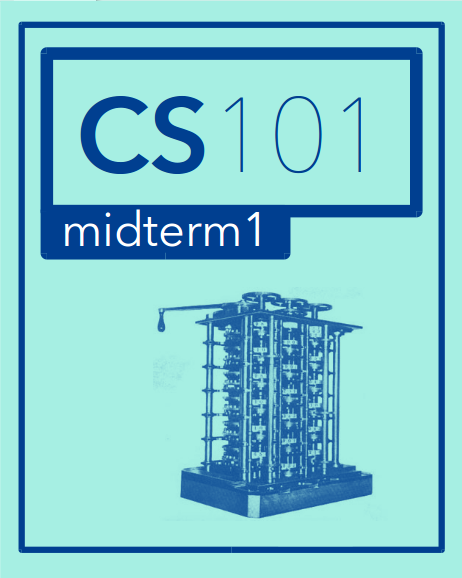
\includegraphics[width=2in]{../img/midterm1-header.png}
\end{center}

\bigskip
\noindent
\begin{itemize}
\item \textbf{Be sure to enter your \underline{NetID} and \underline{the code below} on your Scantron}.
\item Do not turn this page until instructed to do so.
\item There are 30 questions, worth 1 point each.
\item Each question has only \textbf{one} correct answer.
\item You must not communicate with other students during this test.
\item No books, notes, or electronic devices are permitted.
\item This is a 60-minute exam.
\item There are several different versions of this exam.
\end{itemize}

\bigskip\bigskip
\noindent
\textbf{\Large 1. Fill in your information:}

\bigskip
{\Large\bf
\begin{tabular}{ll}
Full Name: & \underbar{\hskip 8cm} \\[0.5em]
UIN (Student Number): & \underbar{\hskip 8cm} \\[0.5em]
NetID: & \underbar{\hskip 8cm}
\end{tabular}
}

\bigskip
\bigskip
\noindent
\textbf{\Large 2. Fill in the following answers on the Scantron form:}

%%%%%%%%%%%%%%%%%%%%%%%%%%%%%%%%%%%%%%%%%%%%%%%%%%%%%%%%%
%%%%%%%%%%%%%%%%%%%%%%%%%%%%%%%%%%%%%%%%%%%%%%%%%%%%%%%%%

\begin{enumerate}
\item[92.] C
\item[93.] E
\item[94.] B
\item[95.] A
\item[96.] A
\end{enumerate}

\newpage

% Zone 1


%%%%%%%%%%%%%%%%%%%%%%%%%%%%%%%%%%%%%%%%%%%%%%%%%%%%%%%%%



\newpage
\noindent
1. (1 point)
Consider the following program:
\begin{verbatim}
x=[1,2,3]
def f(a):
    s=""
    a.reverse()
    for i in a:
        s+=str(i)
    return s

x.append(f(x))
\end{verbatim}
What is the \textbf{value} of \texttt{x} after this program is executed?


\begin{enumerate}
\item[(A)] $\bigstar$ 
\begin{verbatim}[3, 2, 1, '321']\end{verbatim}

\item[(B)]
\begin{verbatim}[3, 2, 1]\end{verbatim}

\item[(C)]
\begin{verbatim}[1, 2, 3]\end{verbatim}

\item[(D)]
\begin{verbatim}[1, 2, 3, '321']\end{verbatim}

\item[(E)]
\begin{verbatim}[1, 2, 3, 6]\end{verbatim}

\end{enumerate}

\vspace*{2em}
\hrule
\vspace{2em}

\noindent {\bf Solution.} 
\vspace{2em}
\hrule height 2pt


\newpage
\noindent
2. (1 point)
Consider the following program.
\begin{verbatim}
s="BBCAA"
x=0
y=len(s)-1
while s[x]!=s[y] and x<len(s):
    x+=1
    y-=1
\end{verbatim}
After it is run, what is the final \textbf{value} of \texttt{x}?


\begin{enumerate}
\item[(A)]
\begin{verbatim}3\end{verbatim}

\item[(B)]
\begin{verbatim}4\end{verbatim}

\item[(C)]
\begin{verbatim}0\end{verbatim}

\item[(D)]
\begin{verbatim}1\end{verbatim}

\item[(E)] $\bigstar$ 
\begin{verbatim}2\end{verbatim}

\end{enumerate}

\vspace*{2em}
\hrule
\vspace{2em}

\noindent {\bf Solution.} 
\vspace{2em}
\hrule height 2pt


\newpage
\noindent
3. (1 point)
Consider the following program:
\begin{verbatim}
s="TRIS %i"
t="ISEU"
x=s % len(t)
\end{verbatim}
What is the \textbf{type} of \texttt{x} after this program is executed?


\begin{enumerate}
\item[(A)] $\bigstar$ 
\begin{verbatim}String\end{verbatim}

\item[(B)]
\begin{verbatim}Boolean\end{verbatim}

\item[(C)]
\begin{verbatim}Float\end{verbatim}

\item[(D)]
\begin{verbatim}Integer\end{verbatim}

\item[(E)]
\begin{verbatim}None\end{verbatim}

\end{enumerate}

\vspace*{2em}
\hrule
\vspace{2em}

\noindent {\bf Solution.} 
\vspace{2em}
\hrule height 2pt


\newpage
\noindent
4. (1 point)
Consider the following program:
\begin{verbatim}
pi="3.14159"
e="2.71828"
x=pi*len(e)+pi
\end{verbatim}
What is the \textbf{type} of \texttt{x} after this program is executed?


\begin{enumerate}
\item[(A)] $\bigstar$ 
\begin{verbatim}String\end{verbatim}

\item[(B)]
\begin{verbatim}Boolean\end{verbatim}

\item[(C)]
\begin{verbatim}None\end{verbatim}

\item[(D)]
\begin{verbatim}Float\end{verbatim}

\item[(E)]
\begin{verbatim}Integer\end{verbatim}

\end{enumerate}

\vspace*{2em}
\hrule
\vspace{2em}

\noindent {\bf Solution.} 
\vspace{2em}
\hrule height 2pt


\newpage
\noindent
5. (1 point)
\begin{verbatim}
x=str(3)+"str(3)"
\end{verbatim}
What is the \textbf{value} of \texttt{x} after this program is executed?


\begin{enumerate}
\item[(A)]
\begin{verbatim}33\end{verbatim}

\item[(B)]
None of the other answers are correct.

\item[(C)]
\begin{verbatim}"333"\end{verbatim}

\item[(D)]
\begin{verbatim}"33"\end{verbatim}

\item[(E)] $\bigstar$ 
\begin{verbatim}"3str(3)"\end{verbatim}

\end{enumerate}

\vspace*{2em}
\hrule
\vspace{2em}

\noindent {\bf Solution.} 
\vspace{2em}
\hrule height 2pt


\newpage
\noindent
6. (1 point)
Consider the following program:
\begin{verbatim}
def fix(s):
    a=list(s)
    a.sort()
    return ''.join(a)

x=["one","two","eleven","twelve"]
s1=fix(x[0]+x[-1])
s2=fix(x[1]+x[-2])

if s1<s2:
    x.sort()
elif s1>s2:
    x.reverse()
else:
    x.append("six")
\end{verbatim}
What is the \textbf{value} of \texttt{x} after this program is executed?


\begin{enumerate}
\item[(A)]
\begin{verbatim}['one', 'two', 'eleven', 'twelve']\end{verbatim}

\item[(B)]
\begin{verbatim}['two', 'twelve', 'one', 'eleven', 'six']\end{verbatim}

\item[(C)] $\bigstar$ 
\begin{verbatim}['one', 'two', 'eleven', 'twelve', 'six']\end{verbatim}

\item[(D)]
\begin{verbatim}['twelve', 'eleven', 'two', 'one']\end{verbatim}

\item[(E)]
\begin{verbatim}['eleven', 'one', 'twelve', 'two']\end{verbatim}

\end{enumerate}

\vspace*{2em}
\hrule
\vspace{2em}

\noindent {\bf Solution.} 
\vspace{2em}
\hrule height 2pt


\newpage
\noindent
7. (1 point)
How can the following mathematical equation be implemented as a Python expression? Assume \verb|a|, \verb|b|, and \verb|cos| have already been defined.
$$a^b \cos(a - b)$$


\begin{enumerate}
\item[(A)]
\begin{verbatim}(b^a)cos(a-b)\end{verbatim}

\item[(B)] $\bigstar$ 
\begin{verbatim}(a**b)*cos(a-b)\end{verbatim}

\item[(C)]
None of the other answers are correct.

\item[(D)]
\begin{verbatim}(a**b)cos(a-b)\end{verbatim}

\item[(E)]
\begin{verbatim}(a^b)*cos(a-b)\end{verbatim}

\end{enumerate}

\vspace*{2em}
\hrule
\vspace{2em}

\noindent {\bf Solution.} 
\vspace{2em}
\hrule height 2pt


\newpage
\noindent
8. (1 point)
Consider the following program.
\begin{verbatim}
x=0
i=1
while(i*i)<=9:
    x=x+(i*i)
    i=i+1
\end{verbatim}
After it is run, what is the final \textbf{value} of \texttt{x}?


\begin{enumerate}
\item[(A)]
\begin{verbatim}5\end{verbatim}

\item[(B)]
\begin{verbatim}3\end{verbatim}

\item[(C)] $\bigstar$ 
\begin{verbatim}14\end{verbatim}

\item[(D)]
\begin{verbatim}30\end{verbatim}

\item[(E)]
\begin{verbatim}4\end{verbatim}

\end{enumerate}

\vspace*{2em}
\hrule
\vspace{2em}

\noindent {\bf Solution.} 
\vspace{2em}
\hrule height 2pt


\newpage
\noindent
9. (1 point)
Consider the following incomplete Python program.
\begin{verbatim}
s="".join(["0","1","2","1"])
x=0
for i in range(len(s)-1):
    x+=int(???)
\end{verbatim}
What should replace the three question marks so the resulting value of \texttt{x} is 34?


\begin{enumerate}
\item[(A)]
\begin{verbatim}s[i:i-1]\end{verbatim}

\item[(B)] $\bigstar$ 
\begin{verbatim}s[i:i+2]\end{verbatim}

\item[(C)]
\begin{verbatim}s[i+1:i+2]\end{verbatim}

\item[(D)]
\begin{verbatim}s[i:i+1]\end{verbatim}

\end{enumerate}

\vspace*{2em}
\hrule
\vspace{2em}

\noindent {\bf Solution.} 
\vspace{2em}
\hrule height 2pt


\newpage
\noindent
10. (1 point)
Consider the following program:
\begin{verbatim}
x=[1,2,3,4,5,6,7,8,9]
x=x[2:-2]
i=1
while i <= 3:
    x[i]+=1
    i+=1
\end{verbatim}
What is the \textbf{value} of \texttt{x} after this program is executed?


\begin{enumerate}
\item[(A)]
\begin{verbatim}[3, 5, 7, 7]\end{verbatim}

\item[(B)]
\begin{verbatim}[3, 5, 6, 7, 7, 8]\end{verbatim}

\item[(C)]
\begin{verbatim}[2, 4, 5, 6, 7, 7]\end{verbatim}

\item[(D)] $\bigstar$ 
\begin{verbatim}[3, 5, 6, 7, 7]\end{verbatim}

\item[(E)]
\begin{verbatim}[2, 4, 5, 5, 7, 7]\end{verbatim}

\end{enumerate}

\vspace*{2em}
\hrule
\vspace{2em}

\noindent {\bf Solution.} 
\vspace{2em}
\hrule height 2pt


\newpage
\noindent
11. (1 point)
Consider the following program:
\begin{verbatim}
a=["merlin","sir agravaine","king pellinore"]
b=[ ]
for i in range(0,4):
    b.append(a[0-i].title())
\end{verbatim}
What is the \textbf{value} of b after this program is executed?


\begin{enumerate}
\item[(A)]
\begin{verbatim}['King Pellinore', 'Sir Agravaine', 'Merlin']\end{verbatim}

\item[(B)]
\begin{verbatim}['Merlin', 'King Pellinore', 'Sir Agravaine']\end{verbatim}

\item[(C)]
\begin{verbatim}[ ]\end{verbatim}

\item[(D)] $\bigstar$ 
\begin{verbatim}['Merlin', 'King Pellinore', 'Sir Agravaine', 'Merlin']\end{verbatim}

\item[(E)]
\begin{verbatim}['Merlin', 'Sir Agravaine', 'King Pellinore', 'Merlin']\end{verbatim}

\end{enumerate}

\vspace*{2em}
\hrule
\vspace{2em}

\noindent {\bf Solution.} 
\vspace{2em}
\hrule height 2pt


\newpage
\noindent
12. (1 point)
Consider the following program:
\begin{verbatim}
s="ECTOR"
t="GAWAIN"
x=(len(s)/(len(t)-1))+1
\end{verbatim}
What is the \textbf{type} of \texttt{x} after this program is executed?


\begin{enumerate}
\item[(A)]
\begin{verbatim}Integer\end{verbatim}

\item[(B)] $\bigstar$ 
\begin{verbatim}Float\end{verbatim}

\item[(C)]
\begin{verbatim}String\end{verbatim}

\item[(D)]
\begin{verbatim}None\end{verbatim}

\item[(E)]
\begin{verbatim}Boolean\end{verbatim}

\end{enumerate}

\vspace*{2em}
\hrule
\vspace{2em}

\noindent {\bf Solution.} 
\vspace{2em}
\hrule height 2pt


\newpage
\noindent
13. (1 point)
Consider the following Python program.
\begin{verbatim}
e=[1,3,5,7,9,11]
d=[0,0,0]
for i in range(0,len(e)):
    d[i%3]+=e[i]
x=d[1]
\end{verbatim}
After it is run, what is the final \textbf{value} of \texttt{x}?


\begin{enumerate}
\item[(A)]
\begin{verbatim}16\end{verbatim}

\item[(B)]
\begin{verbatim}0\end{verbatim}

\item[(C)]
\begin{verbatim}3\end{verbatim}

\item[(D)]
\begin{verbatim}8\end{verbatim}

\item[(E)] $\bigstar$ 
\begin{verbatim}12\end{verbatim}

\end{enumerate}

\vspace*{2em}
\hrule
\vspace{2em}

\noindent {\bf Solution.} 
\vspace{2em}
\hrule height 2pt


\newpage
\noindent
14. (1 point)
Consider the following program:
\begin{verbatim}
s="Calvin"
i=0
x=-1
while i<len(s):
    if s[i]=='b':
        x=i
    i+=1
\end{verbatim}
What is the \textbf{value} of \texttt{x} after this program is executed?


\begin{enumerate}
\item[(A)]
\begin{verbatim}0\end{verbatim}

\item[(B)]
\begin{verbatim}5\end{verbatim}

\item[(C)] $\bigstar$ 
\begin{verbatim}-1\end{verbatim}

\item[(D)]
\begin{verbatim}3\end{verbatim}

\item[(E)]
\begin{verbatim}6\end{verbatim}

\end{enumerate}

\vspace*{2em}
\hrule
\vspace{2em}

\noindent {\bf Solution.} 
\vspace{2em}
\hrule height 2pt


\newpage
\noindent
15. (1 point)
Evaluate the following expression:
\begin{verbatim}
len("ABCDE"[1:4])
\end{verbatim}
What value is produced?


\begin{enumerate}
\item[(A)]
5

\item[(B)] $\bigstar$ 
3

\item[(C)]
4

\item[(D)]
1

\end{enumerate}

\vspace*{2em}
\hrule
\vspace{2em}

\noindent {\bf Solution.} 
\vspace{2em}
\hrule height 2pt


\newpage
\noindent
16. (1 point)
Consider the following incomplete function.
\begin{verbatim}
def isdivisible(m,n):
    if ???:
        return False
    else:
        return True
\end{verbatim}
The function is intended to return True if the input parameter m is evenly divisible by the parameter n and False otherwise. For example, \verb|isdivisible(4,2)| should return \verb|True|, but \verb|isdivisible(5,3)| should return \verb|False|. What should replace the three question marks to complete the function?


\begin{enumerate}
\item[(A)]
\begin{verbatim}(n // m) == 0 \end{verbatim}

\item[(B)]
\begin{verbatim}(m // n) != 0 \end{verbatim}

\item[(C)]
\begin{verbatim}(n % m) == 0 \end{verbatim}

\item[(D)] $\bigstar$ 
\begin{verbatim}(m % n) != 0 \end{verbatim}

\end{enumerate}

\vspace*{2em}
\hrule
\vspace{2em}

\noindent {\bf Solution.} 
\vspace{2em}
\hrule height 2pt


\newpage
\noindent
17. (1 point)
Consider the following program:
\begin{verbatim}
x=0
for i in range(2,7):
    if i%3==0:
        x+=3
    elif i%2==0:
        x+=2
    else:
        x+=1
\end{verbatim}
What is the \textbf{value} of \texttt{x} after this program is executed?


\begin{enumerate}
\item[(A)] $\bigstar$ 
\begin{verbatim}11\end{verbatim}

\item[(B)]
\begin{verbatim}14\end{verbatim}

\item[(C)]
\begin{verbatim}12\end{verbatim}

\item[(D)]
\begin{verbatim}10\end{verbatim}

\item[(E)]
\begin{verbatim}13\end{verbatim}

\end{enumerate}

\vspace*{2em}
\hrule
\vspace{2em}

\noindent {\bf Solution.} 
\vspace{2em}
\hrule height 2pt


\newpage
\noindent
18. (1 point)
What is the result of the following expression?
\begin{verbatim}
[ 1, 2, 3 ] * 3.0
\end{verbatim}


\begin{enumerate}
\item[(A)]
\begin{verbatim}[3, 6, 9]\end{verbatim}

\item[(B)]
\begin{verbatim}None of the above.\end{verbatim}

\item[(C)]
\begin{verbatim}[3.0, 6.0, 9.0]\end{verbatim}

\item[(D)] $\bigstar$ 
\begin{verbatim}[1, 2, 3, 1, 2, 3, 1, 2, 3]\end{verbatim}

\item[(E)]
\begin{verbatim}[1.0, 2.0, 3.0, 1.0, 2.0, 3.0, 1.0, 2.0, 3.0]\end{verbatim}

\end{enumerate}

\vspace*{2em}
\hrule
\vspace{2em}

\noindent {\bf Solution.} 
\vspace{2em}
\hrule height 2pt


\newpage
\noindent
19. (1 point)
Consider the following program:
\begin{verbatim}
s="-B-O-R-S-"
x=s.split("-")[2:-2]
\end{verbatim}
What is the \textbf{value} of \texttt{x} after this program is executed?


\begin{enumerate}
\item[(A)]
\begin{verbatim}False\end{verbatim}

\item[(B)] $\bigstar$ 
\begin{verbatim}['O', 'R']\end{verbatim}

\item[(C)]
\begin{verbatim}''\end{verbatim}

\item[(D)]
\begin{verbatim}'ORS'\end{verbatim}

\item[(E)]
\begin{verbatim}None\end{verbatim}

\end{enumerate}

\vspace*{2em}
\hrule
\vspace{2em}

\noindent {\bf Solution.} 
\vspace{2em}
\hrule height 2pt


\newpage
\noindent
20. (1 point)
Consider the following program.
\begin{verbatim}
x=[]
for j in range(0,5):
    if (j%3)==0:
        x.append("-")
    if (j%4)==0:
        x.append("*")
\end{verbatim}
After it is run, what is the final \textbf{value} of \texttt{x}?


\begin{enumerate}
\item[(A)] $\bigstar$ 
\begin{verbatim}["-","*","-","*"]\end{verbatim}

\item[(B)]
None of the other answers are correct.

\item[(C)]
\begin{verbatim}["*","-","*"]\end{verbatim}

\item[(D)]
\begin{verbatim}["-","*"]\end{verbatim}

\item[(E)]
\begin{verbatim}["*","-","*"]\end{verbatim}

\end{enumerate}

\vspace*{2em}
\hrule
\vspace{2em}

\noindent {\bf Solution.} 
\vspace{2em}
\hrule height 2pt


\newpage
\noindent
21. (1 point)
Consider the following program:
\begin{verbatim}
i=3
x=2
while i < 7:
    x+=i
    i+=2
\end{verbatim}
What is the \textbf{value} of \texttt{x} after this program is executed?


\begin{enumerate}
\item[(A)]
\begin{verbatim}13\end{verbatim}

\item[(B)]
\begin{verbatim}11\end{verbatim}

\item[(C)]
\begin{verbatim}12\end{verbatim}

\item[(D)]
\begin{verbatim}14\end{verbatim}

\item[(E)] $\bigstar$ 
\begin{verbatim}10\end{verbatim}

\end{enumerate}

\vspace*{2em}
\hrule
\vspace{2em}

\noindent {\bf Solution.} 
\vspace{2em}
\hrule height 2pt


\newpage
\noindent
22. (1 point)
Consider the following program.
\begin{verbatim}
def artificing(s):
    return s+"%i" % 2
    return s*2
    return s

s=artificing("MERLIN")
\end{verbatim}
After it is run, what is the final \textbf{value} of s?


\begin{enumerate}
\item[(A)]
\begin{verbatim}0\end{verbatim}

\item[(B)]
\begin{verbatim}None\end{verbatim}

\item[(C)]
\begin{verbatim}"MERLINMERLIN"\end{verbatim}

\item[(D)]
\begin{verbatim}"MERLIN%i"\end{verbatim}

\item[(E)] $\bigstar$ 
\begin{verbatim}"MERLIN2"\end{verbatim}

\end{enumerate}

\vspace*{2em}
\hrule
\vspace{2em}

\noindent {\bf Solution.} 
\vspace{2em}
\hrule height 2pt


\newpage
\noindent
23. (1 point)
Consider the following program:
\begin{verbatim}
x="KING ARTHUR-MORGANA LEFAY-SIR BEDIVERE".split("-")
y=x
y.reverse()
\end{verbatim}
What is the \textbf{value} of \texttt{x} after this program is executed?


\begin{enumerate}
\item[(A)]
\begin{verbatim}None\end{verbatim}

\item[(B)] $\bigstar$ 
\begin{verbatim}['SIR BEDIVERE', 'MORGANA LEFAY', 'KING ARTHUR']\end{verbatim}

\item[(C)]
\begin{verbatim}['KING', 'ARTHUR-MORGANA', 'LEFAY-SIR', 'BEDIVERE']\end{verbatim}

\item[(D)]
\begin{verbatim}['BEDIVERE', 'LEFAY-SIR', 'ARTHUR-MORGANA', 'KING']\end{verbatim}

\item[(E)]
\begin{verbatim}['KING ARTHUR', 'MORGANA LEFAY', 'SIR BEDIVERE']\end{verbatim}

\end{enumerate}

\vspace*{2em}
\hrule
\vspace{2em}

\noindent {\bf Solution.} 
\vspace{2em}
\hrule height 2pt


\newpage
\noindent
24. (1 point)
For this problem, you should compose a function which accomplishes a given task using the available code blocks arranged in the correct functional order.  \emph{We ignore indentation for this problem.}

\texttt{find\_max} should accept a \texttt{list} and return the value of the maximum item in the \texttt{list}.  (\texttt{None} is always the lowest value in any numeric comparison, so you may use it as an initializer.)

\begin{verbatim}
def find_max(my_list):
\end{verbatim}

\begin{enumerate}[1]
\item \texttt{max\_val = i}
\item \texttt{max\_val = None}
\item \texttt{for i in range(len(my\_list)):}
\item \texttt{if i > max\_val:}
\item \texttt{max\_val = my\_list[i]}
\item \texttt{return max\_val}
\item \texttt{for i in range(my\_list):}
\item \texttt{if my\_list[i] > max\_val:}
\item \texttt{print(max\_val)}
\end{enumerate}



\begin{enumerate}
\item[(A)]
2, 7, 4, 5, 6

\item[(B)]
2, 3, 8, 1, 6

\item[(C)]
3, 2, 8, 5, 9

\item[(D)] $\bigstar$ 
2, 3, 8, 5, 6

\item[(E)]
2, 3, 4, 1, 6

\end{enumerate}

\vspace*{2em}
\hrule
\vspace{2em}

\noindent {\bf Solution.} 
\vspace{2em}
\hrule height 2pt


\newpage
\noindent
25. (1 point)
Consider the following program:
\begin{verbatim}
x=3
a=5
if (a%3)==2:
    x=x**3
elif(a%3)==1:
    x=x**2
else:
    x=x**1
\end{verbatim}
What is the \textbf{value} of \texttt{x} after this program is executed?


\begin{enumerate}
\item[(A)]
\begin{verbatim}9\end{verbatim}

\item[(B)]
\begin{verbatim}3\end{verbatim}

\item[(C)]
None of the other answers are correct.

\item[(D)] $\bigstar$ 
\begin{verbatim}27\end{verbatim}

\item[(E)]
\begin{verbatim}1\end{verbatim}

\end{enumerate}

\vspace*{2em}
\hrule
\vspace{2em}

\noindent {\bf Solution.} 
\vspace{2em}
\hrule height 2pt


\newpage
\noindent
26. (1 point)
Consider the following program.
\begin{verbatim}
kay = 2
wart = 3

def knight(kay,wart):
    wart += 2
    kay += 3
    return wart + kay

wart = knight(kay, kay) + knight(wart, wart)
\end{verbatim}
After it is run, what is the final \textbf{value} of \texttt{wart}?


\begin{enumerate}
\item[(A)]
\begin{verbatim}2\end{verbatim}

\item[(B)]
\begin{verbatim}5\end{verbatim}

\item[(C)] $\bigstar$ 
None of the other answers are correct.

\item[(D)]
\begin{verbatim}3\end{verbatim}

\end{enumerate}

\vspace*{2em}
\hrule
\vspace{2em}

\noindent {\bf Solution.} 
\vspace{2em}
\hrule height 2pt


\newpage
\noindent
27. (1 point)
Consider the following program:
\begin{verbatim}
a=3
b=4
if a!=b:
    a=b
elif a==4:
    a=5
else:
    b=a
\end{verbatim}
What is the \textbf{value} of a after this program is executed?


\begin{enumerate}
\item[(A)]
None of the other answers are correct.

\item[(B)] $\bigstar$ 
\begin{verbatim}4\end{verbatim}

\item[(C)]
\begin{verbatim}3\end{verbatim}

\item[(D)]
\begin{verbatim}7\end{verbatim}

\item[(E)]
\begin{verbatim}5\end{verbatim}

\end{enumerate}

\vspace*{2em}
\hrule
\vspace{2em}

\noindent {\bf Solution.} 
\vspace{2em}
\hrule height 2pt


\newpage
\noindent
28. (1 point)
Consider the following incomplete program.
\begin{verbatim}
sum=0
for i in range(0,100):
    ???

\end{verbatim}
The program is intended to sum all of the integers between 1 and 100 (inclusive). What should replace the three question marks to complete the program?


\begin{enumerate}
\item[(A)]
\begin{verbatim}sum=sum+i \end{verbatim}

\item[(B)]
\begin{verbatim}sum=sum+1\end{verbatim}

\item[(C)] $\bigstar$ 
\begin{verbatim}sum=sum+i+1 \end{verbatim}

\item[(D)]
\begin{verbatim}sum+1=sum \end{verbatim}

\end{enumerate}

\vspace*{2em}
\hrule
\vspace{2em}

\noindent {\bf Solution.} 
\vspace{2em}
\hrule height 2pt


\newpage
\noindent
29. (1 point)
Evaluate the following expression:
\begin{verbatim}
[1,2]+[len("3")]
\end{verbatim}
What value is produced?


\begin{enumerate}
\item[(A)]
\begin{verbatim}[1,2,"3"]\end{verbatim}

\item[(B)]
\begin{verbatim}[1,2,1,2,1,2]\end{verbatim}

\item[(C)] $\bigstar$ 
\begin{verbatim}[1,2,1]\end{verbatim}

\item[(D)]
\begin{verbatim}[1,2,3]\end{verbatim}

\end{enumerate}

\vspace*{2em}
\hrule
\vspace{2em}

\noindent {\bf Solution.} 
\vspace{2em}
\hrule height 2pt


\newpage
\noindent
30. (1 point)
Consider the following program:
\begin{verbatim}
a=["A","C","C","I","O"]
a.sort()
a[0]=a[-1]
x=""
for e in a:
    x=x+e
\end{verbatim}
What is the \textbf{value} of \texttt{x} after this program is executed?


\begin{enumerate}
\item[(A)]
\begin{verbatim}"ACCOA"\end{verbatim}

\item[(B)]
None of the other answers are correct.

\item[(C)]
\begin{verbatim}"ACCIA"\end{verbatim}

\item[(D)]
\begin{verbatim}"ICCOI"\end{verbatim}

\item[(E)] $\bigstar$ 
\begin{verbatim}"OCCIO"\end{verbatim}

\end{enumerate}

\vspace*{2em}
\hrule
\vspace{2em}

\noindent {\bf Solution.} 
\vspace{2em}
\hrule height 2pt

%%%%%%%%%%%%%%%%%%%%%%%%%%%%%%%%%%%%%%%%%%%%%%%%%%%%%%%%%%%%%%%%%%%%%%
%%%%%%%%%%%%%%%%%%%%%%%%%%%%%%%%%%%%%%%%%%%%%%%%%%%%%%%%%%%%%%%%%%%%%%
%%%%%%%%%%%%%%%%%%%%%%%%%%%%%%%%%%%%%%%%%%%%%%%%%%%%%%%%%%%%%%%%%%%%%%
%%%%%%%%%%%%%%%%%%%%%%%%%%%%%%%%%%%%%%%%%%%%%%%%%%%%%%%%%%%%%%%%%%%%%%
% Exam number 49

\message{Exam 49/50}
\cleardoublepage
\setcounter{page}{1}


\begin{center}
%\textbf{\Large CS 101 Midterm \#1}
%
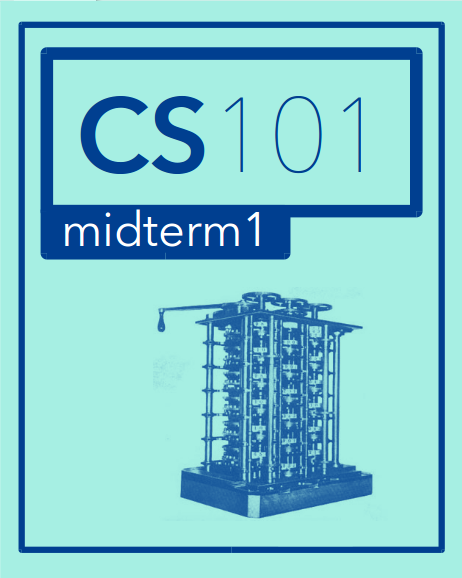
\includegraphics[width=2in]{../img/midterm1-header.png}
\end{center}

\bigskip
\noindent
\begin{itemize}
\item \textbf{Be sure to enter your \underline{NetID} and \underline{the code below} on your Scantron}.
\item Do not turn this page until instructed to do so.
\item There are 30 questions, worth 1 point each.
\item Each question has only \textbf{one} correct answer.
\item You must not communicate with other students during this test.
\item No books, notes, or electronic devices are permitted.
\item This is a 60-minute exam.
\item There are several different versions of this exam.
\end{itemize}

\bigskip\bigskip
\noindent
\textbf{\Large 1. Fill in your information:}

\bigskip
{\Large\bf
\begin{tabular}{ll}
Full Name: & \underbar{\hskip 8cm} \\[0.5em]
UIN (Student Number): & \underbar{\hskip 8cm} \\[0.5em]
NetID: & \underbar{\hskip 8cm}
\end{tabular}
}

\bigskip
\bigskip
\noindent
\textbf{\Large 2. Fill in the following answers on the Scantron form:}

%%%%%%%%%%%%%%%%%%%%%%%%%%%%%%%%%%%%%%%%%%%%%%%%%%%%%%%%%
%%%%%%%%%%%%%%%%%%%%%%%%%%%%%%%%%%%%%%%%%%%%%%%%%%%%%%%%%

\begin{enumerate}
\item[92.] D
\item[93.] E
\item[94.] B
\item[95.] B
\item[96.] B
\end{enumerate}

\newpage

% Zone 1


%%%%%%%%%%%%%%%%%%%%%%%%%%%%%%%%%%%%%%%%%%%%%%%%%%%%%%%%%



\newpage
\noindent
1. (1 point)
For this problem, you should compose a function which accomplishes a given task using the available code blocks arranged in the correct functional order.  \emph{We ignore indentation for this problem.}

\texttt{find\_max} should accept a \texttt{list} and return the value of the maximum item in the \texttt{list}.  (\texttt{None} is always the lowest value in any numeric comparison, so you may use it as an initializer.)

\begin{verbatim}
def find_max(my_list):
\end{verbatim}

\begin{enumerate}[1]
\item \texttt{max\_val = i}
\item \texttt{max\_val = None}
\item \texttt{for i in range(len(my\_list)):}
\item \texttt{if i > max\_val:}
\item \texttt{max\_val = my\_list[i]}
\item \texttt{return max\_val}
\item \texttt{for i in range(my\_list):}
\item \texttt{if my\_list[i] > max\_val:}
\item \texttt{print(max\_val)}
\end{enumerate}



\begin{enumerate}
\item[(A)]
2, 3, 4, 1, 6

\item[(B)] $\bigstar$ 
2, 3, 8, 5, 6

\item[(C)]
2, 3, 8, 1, 6

\item[(D)]
3, 2, 8, 5, 9

\item[(E)]
2, 7, 4, 5, 6

\end{enumerate}

\vspace*{2em}
\hrule
\vspace{2em}

\noindent {\bf Solution.} 
\vspace{2em}
\hrule height 2pt


\newpage
\noindent
2. (1 point)
Evaluate the following expression:
\begin{verbatim}
len("ABCDE"[1:4])
\end{verbatim}
What value is produced?


\begin{enumerate}
\item[(A)] $\bigstar$ 
3

\item[(B)]
4

\item[(C)]
5

\item[(D)]
1

\end{enumerate}

\vspace*{2em}
\hrule
\vspace{2em}

\noindent {\bf Solution.} 
\vspace{2em}
\hrule height 2pt


\newpage
\noindent
3. (1 point)
Consider the following program:
\begin{verbatim}
x=3
a=5
if (a%3)==2:
    x=x**3
elif(a%3)==1:
    x=x**2
else:
    x=x**1
\end{verbatim}
What is the \textbf{value} of \texttt{x} after this program is executed?


\begin{enumerate}
\item[(A)]
\begin{verbatim}1\end{verbatim}

\item[(B)]
\begin{verbatim}3\end{verbatim}

\item[(C)]
None of the other answers are correct.

\item[(D)]
\begin{verbatim}9\end{verbatim}

\item[(E)] $\bigstar$ 
\begin{verbatim}27\end{verbatim}

\end{enumerate}

\vspace*{2em}
\hrule
\vspace{2em}

\noindent {\bf Solution.} 
\vspace{2em}
\hrule height 2pt


\newpage
\noindent
4. (1 point)
Consider the following program.
\begin{verbatim}
x=[]
for j in range(0,5):
    if (j%4)==0:
        x.append("-")
    if (j%5)==0:
        x.append("*")
\end{verbatim}
After it is run, what is the final \textbf{value} of \texttt{x}?


\begin{enumerate}
\item[(A)]
\begin{verbatim}["-","*"]\end{verbatim}

\item[(B)] $\bigstar$ 
\begin{verbatim}["-","*","-"]\end{verbatim}

\item[(C)]
None of the other answers are correct.

\item[(D)]
\begin{verbatim}["-","*","*"]\end{verbatim}

\item[(E)]
\begin{verbatim}["-","-","*"]\end{verbatim}

\end{enumerate}

\vspace*{2em}
\hrule
\vspace{2em}

\noindent {\bf Solution.} 
\vspace{2em}
\hrule height 2pt


\newpage
\noindent
5. (1 point)
Consider the following program:
\begin{verbatim}
x=[1,2,3]
def f(a):
    s=""
    a.reverse()
    for i in a:
        s+=str(i)
    return s

x.append(f(x))
\end{verbatim}
What is the \textbf{value} of \texttt{x} after this program is executed?


\begin{enumerate}
\item[(A)]
\begin{verbatim}[1, 2, 3, '321']\end{verbatim}

\item[(B)]
\begin{verbatim}[1, 2, 3]\end{verbatim}

\item[(C)] $\bigstar$ 
\begin{verbatim}[3, 2, 1, '321']\end{verbatim}

\item[(D)]
\begin{verbatim}[1, 2, 3, 6]\end{verbatim}

\item[(E)]
\begin{verbatim}[3, 2, 1]\end{verbatim}

\end{enumerate}

\vspace*{2em}
\hrule
\vspace{2em}

\noindent {\bf Solution.} 
\vspace{2em}
\hrule height 2pt


\newpage
\noindent
6. (1 point)
Consider the following program:
\begin{verbatim}
def fix(s):
    a=list(s)
    a.sort()
    return ''.join(a)

x=["one","two","eleven","twelve"]
s1=fix(x[0]+x[-1])
s2=fix(x[1]+x[-2])

if s1==s2:
    x.sort()
elif s1<s2:
    x.reverse()
else:
    x.append("six")
\end{verbatim}
What is the \textbf{value} of \texttt{x} after this program is executed?


\begin{enumerate}
\item[(A)]
\begin{verbatim}['one', 'two', 'eleven', 'twelve', 'six']\end{verbatim}

\item[(B)]
\begin{verbatim}['one', 'two', 'eleven', 'twelve']\end{verbatim}

\item[(C)]
\begin{verbatim}['two', 'twelve', 'one', 'eleven', 'six']\end{verbatim}

\item[(D)]
\begin{verbatim}['twelve', 'eleven', 'two', 'one']\end{verbatim}

\item[(E)] $\bigstar$ 
\begin{verbatim}['eleven', 'one', 'twelve', 'two']\end{verbatim}

\end{enumerate}

\vspace*{2em}
\hrule
\vspace{2em}

\noindent {\bf Solution.} 
\vspace{2em}
\hrule height 2pt


\newpage
\noindent
7. (1 point)
Consider the following program:
\begin{verbatim}
i=3
x=2
while i < 7:
    x+=i
    i+=2
\end{verbatim}
What is the \textbf{value} of \texttt{x} after this program is executed?


\begin{enumerate}
\item[(A)]
\begin{verbatim}12\end{verbatim}

\item[(B)]
\begin{verbatim}11\end{verbatim}

\item[(C)]
\begin{verbatim}13\end{verbatim}

\item[(D)]
\begin{verbatim}14\end{verbatim}

\item[(E)] $\bigstar$ 
\begin{verbatim}10\end{verbatim}

\end{enumerate}

\vspace*{2em}
\hrule
\vspace{2em}

\noindent {\bf Solution.} 
\vspace{2em}
\hrule height 2pt


\newpage
\noindent
8. (1 point)
Consider the following Python program.
\begin{verbatim}
e=[1,3,5,7,9,11]
d=[0,0,0]
for i in range(0,len(e)):
    d[i%3]+=e[i]
x=d[1]
\end{verbatim}
After it is run, what is the final \textbf{value} of \texttt{x}?


\begin{enumerate}
\item[(A)] $\bigstar$ 
\begin{verbatim}12\end{verbatim}

\item[(B)]
\begin{verbatim}16\end{verbatim}

\item[(C)]
\begin{verbatim}8\end{verbatim}

\item[(D)]
\begin{verbatim}3\end{verbatim}

\item[(E)]
\begin{verbatim}0\end{verbatim}

\end{enumerate}

\vspace*{2em}
\hrule
\vspace{2em}

\noindent {\bf Solution.} 
\vspace{2em}
\hrule height 2pt


\newpage
\noindent
9. (1 point)
Consider the following program:
\begin{verbatim}
x=0
for i in range(4,10):
    if i%3==0:
        x+=3
    elif i%2==0:
        x+=2
    else:
        x+=1
\end{verbatim}
What is the \textbf{value} of \texttt{x} after this program is executed?


\begin{enumerate}
\item[(A)]
\begin{verbatim}11\end{verbatim}

\item[(B)] $\bigstar$ 
\begin{verbatim}12\end{verbatim}

\item[(C)]
\begin{verbatim}13\end{verbatim}

\item[(D)]
\begin{verbatim}14\end{verbatim}

\item[(E)]
\begin{verbatim}10\end{verbatim}

\end{enumerate}

\vspace*{2em}
\hrule
\vspace{2em}

\noindent {\bf Solution.} 
\vspace{2em}
\hrule height 2pt


\newpage
\noindent
10. (1 point)
What is the result of the following expression?
\begin{verbatim}
[ 1, 2, 3 ] * 3
\end{verbatim}


\begin{enumerate}
\item[(A)]
\begin{verbatim}[3, 6, 9]\end{verbatim}

\item[(B)]
\begin{verbatim}[3.0, 6.0, 9.0]\end{verbatim}

\item[(C)] $\bigstar$ 
\begin{verbatim}[1, 2, 3, 1, 2, 3, 1, 2, 3]\end{verbatim}

\item[(D)]
\begin{verbatim}[1.0, 2.0, 3.0, 1.0, 2.0, 3.0, 1.0, 2.0, 3.0]\end{verbatim}

\item[(E)]
\begin{verbatim}(3, 6, 9)\end{verbatim}

\end{enumerate}

\vspace*{2em}
\hrule
\vspace{2em}

\noindent {\bf Solution.} 
\vspace{2em}
\hrule height 2pt


\newpage
\noindent
11. (1 point)
Consider the following program:
\begin{verbatim}
s="G+R+A+I+L"
x=s.split("+")[1:-2]
\end{verbatim}
What is the \textbf{value} of \texttt{x} after this program is executed?


\begin{enumerate}
\item[(A)]
\begin{verbatim}False\end{verbatim}

\item[(B)]
\begin{verbatim}None\end{verbatim}

\item[(C)]
\begin{verbatim}'RAI'\end{verbatim}

\item[(D)]
\begin{verbatim}3\end{verbatim}

\item[(E)] $\bigstar$ 
\begin{verbatim}['R','A']\end{verbatim}

\end{enumerate}

\vspace*{2em}
\hrule
\vspace{2em}

\noindent {\bf Solution.} 
\vspace{2em}
\hrule height 2pt


\newpage
\noindent
12. (1 point)
Consider the following incomplete function.
\begin{verbatim}
def ismultiple(m,n):
    if ???:
        return False
    else:
        return True
\end{verbatim}
The function is intended to return True if the input parameter m is a multiple of parameter n and False otherwise. For example, \verb|ismultiple(4,2)| should return \verb|True|, but \verb|ismultiple(5,3)| should return \verb|False|. What should replace the three question marks to complete the function?


\begin{enumerate}
\item[(A)]
\begin{verbatim}(m // n) != 0 \end{verbatim}

\item[(B)] $\bigstar$ 
\begin{verbatim}(m % n) != 0 \end{verbatim}

\item[(C)]
\begin{verbatim}(n % m) == 0 \end{verbatim}

\item[(D)]
\begin{verbatim}(n // m) == 0 \end{verbatim}

\end{enumerate}

\vspace*{2em}
\hrule
\vspace{2em}

\noindent {\bf Solution.} 
\vspace{2em}
\hrule height 2pt


\newpage
\noindent
13. (1 point)
Consider the following program:
\begin{verbatim}
x="KING ARTHUR-MORGANA LEFAY-SIR BEDIVERE".split("-")
y=x
x=y.reverse()
\end{verbatim}
What is the \textbf{value} of \texttt{x} after this program is executed?


\begin{enumerate}
\item[(A)]
\begin{verbatim}['KING', 'ARTHUR-MORGANA', 'LEFAY-SIR', 'BEDIVERE']\end{verbatim}

\item[(B)]
\begin{verbatim}['KING ARTHUR', 'MORGANA LEFAY', 'SIR BEDIVERE']\end{verbatim}

\item[(C)] $\bigstar$ 
\begin{verbatim}None\end{verbatim}

\item[(D)]
\begin{verbatim}['SIR BEDIVERE', 'MORGANA LEFAY', 'KING ARTHUR']\end{verbatim}

\item[(E)]
\begin{verbatim}['BEDIVERE', 'LEFAY-SIR', 'ARTHUR-MORGANA', 'KING']\end{verbatim}

\end{enumerate}

\vspace*{2em}
\hrule
\vspace{2em}

\noindent {\bf Solution.} 
\vspace{2em}
\hrule height 2pt


\newpage
\noindent
14. (1 point)
Consider the following incomplete program.
\begin{verbatim}
sum=0
for i in range(0,100):
    ???

\end{verbatim}
The program is intended to sum all of the integers between 1 and 100 (inclusive). What should replace the three question marks to complete the program?


\begin{enumerate}
\item[(A)]
\begin{verbatim}sum=sum+i \end{verbatim}

\item[(B)]
\begin{verbatim}sum=sum+1\end{verbatim}

\item[(C)] $\bigstar$ 
\begin{verbatim}sum=sum+i+1 \end{verbatim}

\item[(D)]
\begin{verbatim}sum+1=sum \end{verbatim}

\end{enumerate}

\vspace*{2em}
\hrule
\vspace{2em}

\noindent {\bf Solution.} 
\vspace{2em}
\hrule height 2pt


\newpage
\noindent
15. (1 point)
Consider the following program:
\begin{verbatim}
s="ECTOR"
t="GAWAIN"
x=len(str(s.isupper()))-t.find("A")
\end{verbatim}
What is the \textbf{type} of \texttt{x} after this program is executed?


\begin{enumerate}
\item[(A)]
\begin{verbatim}Float\end{verbatim}

\item[(B)]
\begin{verbatim}String\end{verbatim}

\item[(C)]
\begin{verbatim}None\end{verbatim}

\item[(D)]
\begin{verbatim}Boolean\end{verbatim}

\item[(E)] $\bigstar$ 
\begin{verbatim}Integer\end{verbatim}

\end{enumerate}

\vspace*{2em}
\hrule
\vspace{2em}

\noindent {\bf Solution.} 
\vspace{2em}
\hrule height 2pt


\newpage
\noindent
16. (1 point)
Consider the following program:
\begin{verbatim}
a=["merlin","sir agravaine","king pellinore"]
b=[ ]
for i in range(0,4):
    b.append(a[0-i].title())
\end{verbatim}
What is the \textbf{value} of b after this program is executed?


\begin{enumerate}
\item[(A)]
\begin{verbatim}['Merlin', 'Sir Agravaine', 'King Pellinore', 'Merlin']\end{verbatim}

\item[(B)]
\begin{verbatim}['Merlin', 'King Pellinore', 'Sir Agravaine']\end{verbatim}

\item[(C)]
\begin{verbatim}['King Pellinore', 'Sir Agravaine', 'Merlin']\end{verbatim}

\item[(D)] $\bigstar$ 
\begin{verbatim}['Merlin', 'King Pellinore', 'Sir Agravaine', 'Merlin']\end{verbatim}

\item[(E)]
\begin{verbatim}[ ]\end{verbatim}

\end{enumerate}

\vspace*{2em}
\hrule
\vspace{2em}

\noindent {\bf Solution.} 
\vspace{2em}
\hrule height 2pt


\newpage
\noindent
17. (1 point)
Consider the following program:
\begin{verbatim}
s="TRIS %i"
t="ISEU"
x=len(s) % len(t[2:-1])
\end{verbatim}
What is the \textbf{type} of \texttt{x} after this program is executed?


\begin{enumerate}
\item[(A)]
\begin{verbatim}String\end{verbatim}

\item[(B)]
\begin{verbatim}Float\end{verbatim}

\item[(C)] $\bigstar$ 
\begin{verbatim}Integer\end{verbatim}

\item[(D)]
\begin{verbatim}None\end{verbatim}

\item[(E)]
\begin{verbatim}Boolean\end{verbatim}

\end{enumerate}

\vspace*{2em}
\hrule
\vspace{2em}

\noindent {\bf Solution.} 
\vspace{2em}
\hrule height 2pt


\newpage
\noindent
18. (1 point)
Consider the following program:
\begin{verbatim}
s="Calvin"
i=0
x=-1
while i<len(s):
    if s[i]=='b':
        x=i
    i+=1
\end{verbatim}
What is the \textbf{value} of \texttt{x} after this program is executed?


\begin{enumerate}
\item[(A)] $\bigstar$ 
\begin{verbatim}-1\end{verbatim}

\item[(B)]
\begin{verbatim}5\end{verbatim}

\item[(C)]
\begin{verbatim}0\end{verbatim}

\item[(D)]
\begin{verbatim}6\end{verbatim}

\item[(E)]
\begin{verbatim}3\end{verbatim}

\end{enumerate}

\vspace*{2em}
\hrule
\vspace{2em}

\noindent {\bf Solution.} 
\vspace{2em}
\hrule height 2pt


\newpage
\noindent
19. (1 point)
Consider the following program:
\begin{verbatim}
a=["A","C","C","I","O"]
a.sort()
a[0]=a[-1]
x=""
for e in a:
    x=x+e
\end{verbatim}
What is the \textbf{value} of \texttt{x} after this program is executed?


\begin{enumerate}
\item[(A)]
\begin{verbatim}"ACCOA"\end{verbatim}

\item[(B)] $\bigstar$ 
\begin{verbatim}"OCCIO"\end{verbatim}

\item[(C)]
\begin{verbatim}"ICCOI"\end{verbatim}

\item[(D)]
\begin{verbatim}"ACCIA"\end{verbatim}

\item[(E)]
None of the other answers are correct.

\end{enumerate}

\vspace*{2em}
\hrule
\vspace{2em}

\noindent {\bf Solution.} 
\vspace{2em}
\hrule height 2pt


\newpage
\noindent
20. (1 point)
Consider the following program:
\begin{verbatim}
a=3
b=4
if a==3:
    b=a
elif a==4:
    a=5
else:
    a=b
\end{verbatim}
What is the \textbf{value} of a after this program is executed?


\begin{enumerate}
\item[(A)]
\begin{verbatim}5\end{verbatim}

\item[(B)]
None of the other answers are correct.

\item[(C)] $\bigstar$ 
\begin{verbatim}3\end{verbatim}

\item[(D)]
\begin{verbatim}4\end{verbatim}

\item[(E)]
\begin{verbatim}7\end{verbatim}

\end{enumerate}

\vspace*{2em}
\hrule
\vspace{2em}

\noindent {\bf Solution.} 
\vspace{2em}
\hrule height 2pt


\newpage
\noindent
21. (1 point)
How can the following mathematical equation be implemented as a Python expression? Assume \verb|a|, \verb|b|, and \verb|sin| have already been defined.
$$a \sin(a^b - b)$$


\begin{enumerate}
\item[(A)]
\begin{verbatim}a sin(a**b - b)\end{verbatim}

\item[(B)]
None of the other answers are correct.

\item[(C)]
\begin{verbatim}a*sin(a^b - b)\end{verbatim}

\item[(D)]
\begin{verbatim}a*sin(b^a - b)\end{verbatim}

\item[(E)] $\bigstar$ 
\begin{verbatim}a*sin(a**b - b)\end{verbatim}

\end{enumerate}

\vspace*{2em}
\hrule
\vspace{2em}

\noindent {\bf Solution.} 
\vspace{2em}
\hrule height 2pt


\newpage
\noindent
22. (1 point)
Evaluate the following expression:
\begin{verbatim}
[1,2]*len("3")
\end{verbatim}
What value is produced?


\begin{enumerate}
\item[(A)] $\bigstar$ 
\begin{verbatim}[1,2]\end{verbatim}

\item[(B)]
\begin{verbatim}[1,2,1]\end{verbatim}

\item[(C)]
\begin{verbatim}[1,2,3]\end{verbatim}

\item[(D)]
\begin{verbatim}[1,2,1,2,1,2]\end{verbatim}

\end{enumerate}

\vspace*{2em}
\hrule
\vspace{2em}

\noindent {\bf Solution.} 
\vspace{2em}
\hrule height 2pt


\newpage
\noindent
23. (1 point)
Consider the following program.
\begin{verbatim}
kay = 2
wart = 3

def knight(kay,wart):
    wart += 2
    kay += 3
    return wart + kay

kay = knight(wart, kay) + knight(kay, wart)
\end{verbatim}
After it is run, what is the final \textbf{value} of \texttt{kay}?


\begin{enumerate}
\item[(A)] $\bigstar$ 
None of the other answers are correct.

\item[(B)]
\begin{verbatim}5\end{verbatim}

\item[(C)]
\begin{verbatim}2\end{verbatim}

\item[(D)]
\begin{verbatim}3\end{verbatim}

\end{enumerate}

\vspace*{2em}
\hrule
\vspace{2em}

\noindent {\bf Solution.} 
\vspace{2em}
\hrule height 2pt


\newpage
\noindent
24. (1 point)
Consider the following program.
\begin{verbatim}
x=0
i=1
while(i*i)<=9:
    x=x+(i*i)
    i=i+1
\end{verbatim}
After it is run, what is the final \textbf{value} of \texttt{x}?


\begin{enumerate}
\item[(A)]
\begin{verbatim}5\end{verbatim}

\item[(B)] $\bigstar$ 
\begin{verbatim}14\end{verbatim}

\item[(C)]
\begin{verbatim}3\end{verbatim}

\item[(D)]
\begin{verbatim}4\end{verbatim}

\item[(E)]
\begin{verbatim}30\end{verbatim}

\end{enumerate}

\vspace*{2em}
\hrule
\vspace{2em}

\noindent {\bf Solution.} 
\vspace{2em}
\hrule height 2pt


\newpage
\noindent
25. (1 point)
Consider the following incomplete Python program.
\begin{verbatim}
s="".join(["1","0","2","1"])
x=0
for i in range(len(s)-1):
    x+=int(???)
\end{verbatim}
What should replace the three question marks so the resulting value of \texttt{x} is 33?


\begin{enumerate}
\item[(A)]
\begin{verbatim}s[i+1:i+2]\end{verbatim}

\item[(B)] $\bigstar$ 
\begin{verbatim}s[i:i+2]\end{verbatim}

\item[(C)]
\begin{verbatim}s[i:i-1]\end{verbatim}

\item[(D)]
\begin{verbatim}s[i:i+1]\end{verbatim}

\end{enumerate}

\vspace*{2em}
\hrule
\vspace{2em}

\noindent {\bf Solution.} 
\vspace{2em}
\hrule height 2pt


\newpage
\noindent
26. (1 point)
Consider the following program:
\begin{verbatim}
x=str(1.2)*2
\end{verbatim}
What is the \textbf{value} of \texttt{x} after this program is executed?


\begin{enumerate}
\item[(A)]
\begin{verbatim}"1.2*2"\end{verbatim}

\item[(B)]
\begin{verbatim}"2.4"\end{verbatim}

\item[(C)] $\bigstar$ 
\begin{verbatim}"1.21.2"\end{verbatim}

\item[(D)]
\begin{verbatim}2.4\end{verbatim}

\item[(E)]
None of the other answers are correct.

\end{enumerate}

\vspace*{2em}
\hrule
\vspace{2em}

\noindent {\bf Solution.} 
\vspace{2em}
\hrule height 2pt


\newpage
\noindent
27. (1 point)
Consider the following program:
\begin{verbatim}
x=[1,2,3,4,5,6,7,8,9]
x=x[2:-2]
i=1
while i < 3:
    x[i]+=1
    i+=1
\end{verbatim}
What is the \textbf{value} of \texttt{x} after this program is executed?


\begin{enumerate}
\item[(A)] $\bigstar$ 
\begin{verbatim}[3, 5, 6, 6, 7]\end{verbatim}

\item[(B)]
\begin{verbatim}[3, 5, 6, 6]\end{verbatim}

\item[(C)]
\begin{verbatim}[3, 5, 6, 6, 7, 8]\end{verbatim}

\item[(D)]
\begin{verbatim}[2, 4, 5, 5, 6, 7]\end{verbatim}

\item[(E)]
\begin{verbatim}[2, 4, 5, 6, 6, 7]\end{verbatim}

\end{enumerate}

\vspace*{2em}
\hrule
\vspace{2em}

\noindent {\bf Solution.} 
\vspace{2em}
\hrule height 2pt


\newpage
\noindent
28. (1 point)
Consider the following program.
\begin{verbatim}
def artificing(s):
    return s+"%i" % 2
    return s*2
    return s

s=artificing("MERLIN")
\end{verbatim}
After it is run, what is the final \textbf{value} of s?


\begin{enumerate}
\item[(A)]
\begin{verbatim}0\end{verbatim}

\item[(B)] $\bigstar$ 
\begin{verbatim}"MERLIN2"\end{verbatim}

\item[(C)]
\begin{verbatim}None\end{verbatim}

\item[(D)]
\begin{verbatim}"MERLINMERLIN"\end{verbatim}

\item[(E)]
\begin{verbatim}"MERLIN%i"\end{verbatim}

\end{enumerate}

\vspace*{2em}
\hrule
\vspace{2em}

\noindent {\bf Solution.} 
\vspace{2em}
\hrule height 2pt


\newpage
\noindent
29. (1 point)
Consider the following program.
\begin{verbatim}
s="ABCBA"
x=0
y=len(s)-1
while s[x]==s[y] and x<=y:
    x+=1
    y-=1
\end{verbatim}
After it is run, what is the final \textbf{value} of \texttt{x}?


\begin{enumerate}
\item[(A)]
\begin{verbatim}0\end{verbatim}

\item[(B)] $\bigstar$ 
\begin{verbatim}3\end{verbatim}

\item[(C)]
\begin{verbatim}2\end{verbatim}

\item[(D)]
\begin{verbatim}1\end{verbatim}

\item[(E)]
\begin{verbatim}4\end{verbatim}

\end{enumerate}

\vspace*{2em}
\hrule
\vspace{2em}

\noindent {\bf Solution.} 
\vspace{2em}
\hrule height 2pt


\newpage
\noindent
30. (1 point)
Consider the following program:
\begin{verbatim}
pi="3.14159"
e="2.71828"
x=pi in pi*len(e)
\end{verbatim}
What is the \textbf{type} of \texttt{x} after this program is executed?


\begin{enumerate}
\item[(A)]
\begin{verbatim}None\end{verbatim}

\item[(B)]
\begin{verbatim}Integer\end{verbatim}

\item[(C)]
\begin{verbatim}Float\end{verbatim}

\item[(D)]
\begin{verbatim}String\end{verbatim}

\item[(E)] $\bigstar$ 
\begin{verbatim}Boolean\end{verbatim}

\end{enumerate}

\vspace*{2em}
\hrule
\vspace{2em}

\noindent {\bf Solution.} 
\vspace{2em}
\hrule height 2pt

%%%%%%%%%%%%%%%%%%%%%%%%%%%%%%%%%%%%%%%%%%%%%%%%%%%%%%%%%%%%%%%%%%%%%%
%%%%%%%%%%%%%%%%%%%%%%%%%%%%%%%%%%%%%%%%%%%%%%%%%%%%%%%%%%%%%%%%%%%%%%
%%%%%%%%%%%%%%%%%%%%%%%%%%%%%%%%%%%%%%%%%%%%%%%%%%%%%%%%%%%%%%%%%%%%%%
%%%%%%%%%%%%%%%%%%%%%%%%%%%%%%%%%%%%%%%%%%%%%%%%%%%%%%%%%%%%%%%%%%%%%%
% Exam number 50

\message{Exam 50/50}
\cleardoublepage
\setcounter{page}{1}


\begin{center}
%\textbf{\Large CS 101 Midterm \#1}
%
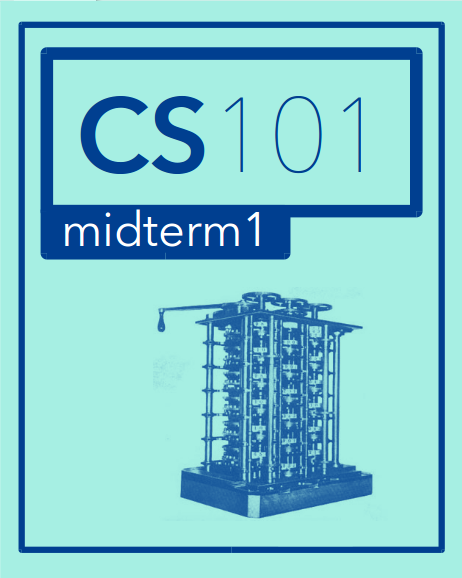
\includegraphics[width=2in]{../img/midterm1-header.png}
\end{center}

\bigskip
\noindent
\begin{itemize}
\item \textbf{Be sure to enter your \underline{NetID} and \underline{the code below} on your Scantron}.
\item Do not turn this page until instructed to do so.
\item There are 30 questions, worth 1 point each.
\item Each question has only \textbf{one} correct answer.
\item You must not communicate with other students during this test.
\item No books, notes, or electronic devices are permitted.
\item This is a 60-minute exam.
\item There are several different versions of this exam.
\end{itemize}

\bigskip\bigskip
\noindent
\textbf{\Large 1. Fill in your information:}

\bigskip
{\Large\bf
\begin{tabular}{ll}
Full Name: & \underbar{\hskip 8cm} \\[0.5em]
UIN (Student Number): & \underbar{\hskip 8cm} \\[0.5em]
NetID: & \underbar{\hskip 8cm}
\end{tabular}
}

\bigskip
\bigskip
\noindent
\textbf{\Large 2. Fill in the following answers on the Scantron form:}

%%%%%%%%%%%%%%%%%%%%%%%%%%%%%%%%%%%%%%%%%%%%%%%%%%%%%%%%%
%%%%%%%%%%%%%%%%%%%%%%%%%%%%%%%%%%%%%%%%%%%%%%%%%%%%%%%%%

\begin{enumerate}
\item[92.] E
\item[93.] E
\item[94.] B
\item[95.] C
\item[96.] C
\end{enumerate}

\newpage

% Zone 1


%%%%%%%%%%%%%%%%%%%%%%%%%%%%%%%%%%%%%%%%%%%%%%%%%%%%%%%%%



\newpage
\noindent
1. (1 point)
Consider the following incomplete program.
\begin{verbatim}
sum=0
for i in range(0,100):
    ???

\end{verbatim}
The program is intended to sum all of the integers between 1 and 100 (inclusive). What should replace the three question marks to complete the program?


\begin{enumerate}
\item[(A)] $\bigstar$ 
\begin{verbatim}sum=sum+i+1 \end{verbatim}

\item[(B)]
\begin{verbatim}sum=sum+i \end{verbatim}

\item[(C)]
\begin{verbatim}sum=sum+1\end{verbatim}

\item[(D)]
\begin{verbatim}sum+1=sum \end{verbatim}

\end{enumerate}

\vspace*{2em}
\hrule
\vspace{2em}

\noindent {\bf Solution.} 
\vspace{2em}
\hrule height 2pt


\newpage
\noindent
2. (1 point)
Consider the following program:
\begin{verbatim}
s="-B-O-R-S-"
x=s.split("-")[2:-2]
\end{verbatim}
What is the \textbf{value} of \texttt{x} after this program is executed?


\begin{enumerate}
\item[(A)] $\bigstar$ 
\begin{verbatim}['O', 'R']\end{verbatim}

\item[(B)]
\begin{verbatim}''\end{verbatim}

\item[(C)]
\begin{verbatim}'ORS'\end{verbatim}

\item[(D)]
\begin{verbatim}None\end{verbatim}

\item[(E)]
\begin{verbatim}False\end{verbatim}

\end{enumerate}

\vspace*{2em}
\hrule
\vspace{2em}

\noindent {\bf Solution.} 
\vspace{2em}
\hrule height 2pt


\newpage
\noindent
3. (1 point)
Consider the following program:
\begin{verbatim}
pi="3.14159"
e="2.71828"
x=pi*len(e)+pi
\end{verbatim}
What is the \textbf{type} of \texttt{x} after this program is executed?


\begin{enumerate}
\item[(A)]
\begin{verbatim}Float\end{verbatim}

\item[(B)] $\bigstar$ 
\begin{verbatim}String\end{verbatim}

\item[(C)]
\begin{verbatim}Boolean\end{verbatim}

\item[(D)]
\begin{verbatim}None\end{verbatim}

\item[(E)]
\begin{verbatim}Integer\end{verbatim}

\end{enumerate}

\vspace*{2em}
\hrule
\vspace{2em}

\noindent {\bf Solution.} 
\vspace{2em}
\hrule height 2pt


\newpage
\noindent
4. (1 point)
Consider the following Python program.
\begin{verbatim}
e=[1,3,5,7,9,11]
d=[0,0,0]
for i in range(0,len(e)):
    d[i%3]+=e[i]
x=d[2]
\end{verbatim}
After it is run, what is the final \textbf{value} of \texttt{x}?


\begin{enumerate}
\item[(A)]
\begin{verbatim}12\end{verbatim}

\item[(B)]
\begin{verbatim}8\end{verbatim}

\item[(C)] $\bigstar$ 
\begin{verbatim}16\end{verbatim}

\item[(D)]
\begin{verbatim}7\end{verbatim}

\item[(E)]
\begin{verbatim}0\end{verbatim}

\end{enumerate}

\vspace*{2em}
\hrule
\vspace{2em}

\noindent {\bf Solution.} 
\vspace{2em}
\hrule height 2pt


\newpage
\noindent
5. (1 point)
What is the result of the following expression?
\begin{verbatim}
[ 1, 2, 3 ] * 3
\end{verbatim}


\begin{enumerate}
\item[(A)]
\begin{verbatim}(3, 6, 9)\end{verbatim}

\item[(B)]
\begin{verbatim}[1.0, 2.0, 3.0, 1.0, 2.0, 3.0, 1.0, 2.0, 3.0]\end{verbatim}

\item[(C)]
\begin{verbatim}[3, 6, 9]\end{verbatim}

\item[(D)]
\begin{verbatim}[3.0, 6.0, 9.0]\end{verbatim}

\item[(E)] $\bigstar$ 
\begin{verbatim}[1, 2, 3, 1, 2, 3, 1, 2, 3]\end{verbatim}

\end{enumerate}

\vspace*{2em}
\hrule
\vspace{2em}

\noindent {\bf Solution.} 
\vspace{2em}
\hrule height 2pt


\newpage
\noindent
6. (1 point)
Consider the following program:
\begin{verbatim}
i=2
x=3
while i < 7:
    x+=i
    i+=2
\end{verbatim}
What is the \textbf{value} of \texttt{x} after this program is executed?


\begin{enumerate}
\item[(A)]
\begin{verbatim}13\end{verbatim}

\item[(B)]
\begin{verbatim}11\end{verbatim}

\item[(C)]
\begin{verbatim}12\end{verbatim}

\item[(D)] $\bigstar$ 
\begin{verbatim}15\end{verbatim}

\item[(E)]
\begin{verbatim}14\end{verbatim}

\end{enumerate}

\vspace*{2em}
\hrule
\vspace{2em}

\noindent {\bf Solution.} 
\vspace{2em}
\hrule height 2pt


\newpage
\noindent
7. (1 point)
How can the following mathematical equation be implemented as a Python expression? Assume \verb|a|, \verb|b|, and \verb|sin| have already been defined.
$$a \sin(a^b - b)$$


\begin{enumerate}
\item[(A)]
\begin{verbatim}a sin(a**b - b)\end{verbatim}

\item[(B)]
None of the other answers are correct.

\item[(C)] $\bigstar$ 
\begin{verbatim}a*sin(a**b - b)\end{verbatim}

\item[(D)]
\begin{verbatim}a*sin(b^a - b)\end{verbatim}

\item[(E)]
\begin{verbatim}a*sin(a^b - b)\end{verbatim}

\end{enumerate}

\vspace*{2em}
\hrule
\vspace{2em}

\noindent {\bf Solution.} 
\vspace{2em}
\hrule height 2pt


\newpage
\noindent
8. (1 point)
Consider the following program:
\begin{verbatim}
x="KING ARTHUR-MORGANA LEFAY-SIR BEDIVERE".split("-")
y=x[:]
y.reverse()
\end{verbatim}
What is the \textbf{value} of \texttt{x} after this program is executed?


\begin{enumerate}
\item[(A)] $\bigstar$ 
\begin{verbatim}['KING ARTHUR', 'MORGANA LEFAY', 'SIR BEDIVERE']\end{verbatim}

\item[(B)]
\begin{verbatim}['BEDIVERE', 'LEFAY-SIR', 'ARTHUR-MORGANA', 'KING']\end{verbatim}

\item[(C)]
\begin{verbatim}['SIR BEDIVERE', 'MORGANA LEFAY', 'KING ARTHUR']\end{verbatim}

\item[(D)]
\begin{verbatim}None\end{verbatim}

\item[(E)]
\begin{verbatim}['KING', 'ARTHUR-MORGANA', 'LEFAY-SIR', 'BEDIVERE']\end{verbatim}

\end{enumerate}

\vspace*{2em}
\hrule
\vspace{2em}

\noindent {\bf Solution.} 
\vspace{2em}
\hrule height 2pt


\newpage
\noindent
9. (1 point)
Evaluate the following expression:
\begin{verbatim}
[1,2]*len("3")
\end{verbatim}
What value is produced?


\begin{enumerate}
\item[(A)]
\begin{verbatim}[1,2,3]\end{verbatim}

\item[(B)] $\bigstar$ 
\begin{verbatim}[1,2]\end{verbatim}

\item[(C)]
\begin{verbatim}[1,2,1]\end{verbatim}

\item[(D)]
\begin{verbatim}[1,2,1,2,1,2]\end{verbatim}

\end{enumerate}

\vspace*{2em}
\hrule
\vspace{2em}

\noindent {\bf Solution.} 
\vspace{2em}
\hrule height 2pt


\newpage
\noindent
10. (1 point)
Consider the following program:
\begin{verbatim}
s="ECTOR"
t="GAWAIN"
x=len(str(s.isupper()))-t.find("A")
\end{verbatim}
What is the \textbf{type} of \texttt{x} after this program is executed?


\begin{enumerate}
\item[(A)]
\begin{verbatim}String\end{verbatim}

\item[(B)]
\begin{verbatim}Boolean\end{verbatim}

\item[(C)] $\bigstar$ 
\begin{verbatim}Integer\end{verbatim}

\item[(D)]
\begin{verbatim}None\end{verbatim}

\item[(E)]
\begin{verbatim}Float\end{verbatim}

\end{enumerate}

\vspace*{2em}
\hrule
\vspace{2em}

\noindent {\bf Solution.} 
\vspace{2em}
\hrule height 2pt


\newpage
\noindent
11. (1 point)
Consider the following program:
\begin{verbatim}
a=["merlin","sir agravaine","king pellinore"]
b=[ ]
for i in range(1,3):
    b.append(a[0-i].title())
\end{verbatim}
What is the \textbf{value} of b after this program is executed?


\begin{enumerate}
\item[(A)]
\begin{verbatim}[ ]\end{verbatim}

\item[(B)]
\begin{verbatim}['King Pellinore', 'Sir Agravaine', 'Merlin']\end{verbatim}

\item[(C)] $\bigstar$ 
\begin{verbatim}['King Pellinore', 'Sir Agravaine']\end{verbatim}

\item[(D)]
\begin{verbatim}['Merlin', 'King Pellinore', 'Sir Agravaine']\end{verbatim}

\item[(E)]
\begin{verbatim}['Sir Agravaine', 'King Pellinore']\end{verbatim}

\end{enumerate}

\vspace*{2em}
\hrule
\vspace{2em}

\noindent {\bf Solution.} 
\vspace{2em}
\hrule height 2pt


\newpage
\noindent
12. (1 point)
Consider the following program:
\begin{verbatim}
x=str("1"*3)
\end{verbatim}
What is the \textbf{value} of \texttt{x} after this program is executed?


\begin{enumerate}
\item[(A)]
None of the other answers are correct.

\item[(B)]
\begin{verbatim}"3"\end{verbatim}

\item[(C)]
\begin{verbatim}111\end{verbatim}

\item[(D)]
\begin{verbatim}3\end{verbatim}

\item[(E)] $\bigstar$ 
\begin{verbatim}"111"\end{verbatim}

\end{enumerate}

\vspace*{2em}
\hrule
\vspace{2em}

\noindent {\bf Solution.} 
\vspace{2em}
\hrule height 2pt


\newpage
\noindent
13. (1 point)
Evaluate the following expression:
\begin{verbatim}
len("ABCD"[0:3])
\end{verbatim}
What value is produced?


\begin{enumerate}
\item[(A)]
2

\item[(B)]
1

\item[(C)] $\bigstar$ 
3

\item[(D)]
4

\end{enumerate}

\vspace*{2em}
\hrule
\vspace{2em}

\noindent {\bf Solution.} 
\vspace{2em}
\hrule height 2pt


\newpage
\noindent
14. (1 point)
Consider the following program:
\begin{verbatim}
x=[1,2,3]
def f(a):
    s=""
    a.reverse()
    for i in a:
        s+=str(i)
    return s

x.append(f(x))
\end{verbatim}
What is the \textbf{value} of \texttt{x} after this program is executed?


\begin{enumerate}
\item[(A)]
\begin{verbatim}[1, 2, 3, 6]\end{verbatim}

\item[(B)] $\bigstar$ 
\begin{verbatim}[3, 2, 1, '321']\end{verbatim}

\item[(C)]
\begin{verbatim}[3, 2, 1]\end{verbatim}

\item[(D)]
\begin{verbatim}[1, 2, 3, '321']\end{verbatim}

\item[(E)]
\begin{verbatim}[1, 2, 3]\end{verbatim}

\end{enumerate}

\vspace*{2em}
\hrule
\vspace{2em}

\noindent {\bf Solution.} 
\vspace{2em}
\hrule height 2pt


\newpage
\noindent
15. (1 point)
Consider the following program.
\begin{verbatim}
s="BBCAA"
x=0
y=len(s)-1
while s[x]!=s[y] and x<len(s):
    x+=1
    y-=1
\end{verbatim}
After it is run, what is the final \textbf{value} of \texttt{x}?


\begin{enumerate}
\item[(A)]
\begin{verbatim}0\end{verbatim}

\item[(B)]
\begin{verbatim}1\end{verbatim}

\item[(C)] $\bigstar$ 
\begin{verbatim}2\end{verbatim}

\item[(D)]
\begin{verbatim}4\end{verbatim}

\item[(E)]
\begin{verbatim}3\end{verbatim}

\end{enumerate}

\vspace*{2em}
\hrule
\vspace{2em}

\noindent {\bf Solution.} 
\vspace{2em}
\hrule height 2pt


\newpage
\noindent
16. (1 point)
Consider the following program:
\begin{verbatim}
x=3
a=5
if (a%3)==2:
    x=x**3
elif(a%3)==1:
    x=x**2
else:
    x=x**1
\end{verbatim}
What is the \textbf{value} of \texttt{x} after this program is executed?


\begin{enumerate}
\item[(A)]
\begin{verbatim}1\end{verbatim}

\item[(B)]
\begin{verbatim}9\end{verbatim}

\item[(C)]
\begin{verbatim}3\end{verbatim}

\item[(D)]
None of the other answers are correct.

\item[(E)] $\bigstar$ 
\begin{verbatim}27\end{verbatim}

\end{enumerate}

\vspace*{2em}
\hrule
\vspace{2em}

\noindent {\bf Solution.} 
\vspace{2em}
\hrule height 2pt


\newpage
\noindent
17. (1 point)
Consider the following program.
\begin{verbatim}
def artificing(s):
    return s*2
    return s+"%i" % 2
    return s

s=artificing("MERLIN")
\end{verbatim}
After it is run, what is the final \textbf{value} of s?


\begin{enumerate}
\item[(A)]
\begin{verbatim}12\end{verbatim}

\item[(B)]
\begin{verbatim}"MERLIN"\end{verbatim}

\item[(C)]
\begin{verbatim}"MERLIN2"\end{verbatim}

\item[(D)] $\bigstar$ 
\begin{verbatim}"MERLINMERLIN"\end{verbatim}

\item[(E)]
\begin{verbatim}None\end{verbatim}

\end{enumerate}

\vspace*{2em}
\hrule
\vspace{2em}

\noindent {\bf Solution.} 
\vspace{2em}
\hrule height 2pt


\newpage
\noindent
18. (1 point)
Consider the following program:
\begin{verbatim}
x=0
for i in range(2,7):
    if i%3==0:
        x+=3
    elif i%2==0:
        x+=2
    else:
        x+=1
\end{verbatim}
What is the \textbf{value} of \texttt{x} after this program is executed?


\begin{enumerate}
\item[(A)] $\bigstar$ 
\begin{verbatim}11\end{verbatim}

\item[(B)]
\begin{verbatim}12\end{verbatim}

\item[(C)]
\begin{verbatim}14\end{verbatim}

\item[(D)]
\begin{verbatim}10\end{verbatim}

\item[(E)]
\begin{verbatim}13\end{verbatim}

\end{enumerate}

\vspace*{2em}
\hrule
\vspace{2em}

\noindent {\bf Solution.} 
\vspace{2em}
\hrule height 2pt


\newpage
\noindent
19. (1 point)
Consider the following incomplete function.
\begin{verbatim}
def ismultiple(m,n):
    if ???:
        return False
    else:
        return True
\end{verbatim}
The function is intended to return True if the input parameter m is a multiple of parameter n and False otherwise. For example, \verb|ismultiple(4,2)| should return \verb|True|, but \verb|ismultiple(5,3)| should return \verb|False|. What should replace the three question marks to complete the function?


\begin{enumerate}
\item[(A)]
\begin{verbatim}(m // n) != 0 \end{verbatim}

\item[(B)]
\begin{verbatim}(n % m) == 0 \end{verbatim}

\item[(C)]
\begin{verbatim}(n // m) == 0 \end{verbatim}

\item[(D)] $\bigstar$ 
\begin{verbatim}(m % n) != 0 \end{verbatim}

\end{enumerate}

\vspace*{2em}
\hrule
\vspace{2em}

\noindent {\bf Solution.} 
\vspace{2em}
\hrule height 2pt


\newpage
\noindent
20. (1 point)
Consider the following program:
\begin{verbatim}
a=["A","C","C","I","O"]
a.sort()
a[0]=a[-1]
x=""
for e in a:
    x=x+e
\end{verbatim}
What is the \textbf{value} of \texttt{x} after this program is executed?


\begin{enumerate}
\item[(A)]
None of the other answers are correct.

\item[(B)] $\bigstar$ 
\begin{verbatim}"OCCIO"\end{verbatim}

\item[(C)]
\begin{verbatim}"ACCIA"\end{verbatim}

\item[(D)]
\begin{verbatim}"ACCOA"\end{verbatim}

\item[(E)]
\begin{verbatim}"ICCOI"\end{verbatim}

\end{enumerate}

\vspace*{2em}
\hrule
\vspace{2em}

\noindent {\bf Solution.} 
\vspace{2em}
\hrule height 2pt


\newpage
\noindent
21. (1 point)
Consider the following incomplete Python program.
\begin{verbatim}
s="".join(["1","0","2","1"])
x=0
for i in range(len(s)-1):
    x+=int(???)
\end{verbatim}
What should replace the three question marks so the resulting value of \texttt{x} is 33?


\begin{enumerate}
\item[(A)] $\bigstar$ 
\begin{verbatim}s[i:i+2]\end{verbatim}

\item[(B)]
\begin{verbatim}s[i:i+1]\end{verbatim}

\item[(C)]
\begin{verbatim}s[i+1:i+2]\end{verbatim}

\item[(D)]
\begin{verbatim}s[i:i-1]\end{verbatim}

\end{enumerate}

\vspace*{2em}
\hrule
\vspace{2em}

\noindent {\bf Solution.} 
\vspace{2em}
\hrule height 2pt


\newpage
\noindent
22. (1 point)
Consider the following program:
\begin{verbatim}
a=3
b=4
if a!=b:
    a=b
elif a==4:
    a=5
else:
    b=a
\end{verbatim}
What is the \textbf{value} of a after this program is executed?


\begin{enumerate}
\item[(A)]
\begin{verbatim}7\end{verbatim}

\item[(B)]
\begin{verbatim}5\end{verbatim}

\item[(C)]
None of the other answers are correct.

\item[(D)] $\bigstar$ 
\begin{verbatim}4\end{verbatim}

\item[(E)]
\begin{verbatim}3\end{verbatim}

\end{enumerate}

\vspace*{2em}
\hrule
\vspace{2em}

\noindent {\bf Solution.} 
\vspace{2em}
\hrule height 2pt


\newpage
\noindent
23. (1 point)
Consider the following program.
\begin{verbatim}
x=1
i=0
while(x*x)<=9:
    i=i+(x*x)
    x=x+1
\end{verbatim}
After it is run, what is the final \textbf{value} of \texttt{x}?


\begin{enumerate}
\item[(A)]
\begin{verbatim}30\end{verbatim}

\item[(B)]
\begin{verbatim}3\end{verbatim}

\item[(C)]
\begin{verbatim}14\end{verbatim}

\item[(D)]
\begin{verbatim}5\end{verbatim}

\item[(E)] $\bigstar$ 
\begin{verbatim}4\end{verbatim}

\end{enumerate}

\vspace*{2em}
\hrule
\vspace{2em}

\noindent {\bf Solution.} 
\vspace{2em}
\hrule height 2pt


\newpage
\noindent
24. (1 point)
For this problem, you should compose a function which accomplishes a given task using the available code blocks arranged in the correct functional order.  \emph{We ignore indentation for this problem.}

\texttt{find\_max} should accept a \texttt{list} and return the value of the maximum item in the \texttt{list}.  (\texttt{None} is always the lowest value in any numeric comparison, so you may use it as an initializer.)

\begin{verbatim}
def find_max(my_list):
\end{verbatim}

\begin{enumerate}[1]
\item \texttt{max\_val = i}
\item \texttt{max\_val = None}
\item \texttt{for i in range(len(my\_list)):}
\item \texttt{if i > max\_val:}
\item \texttt{max\_val = my\_list[i]}
\item \texttt{return max\_val}
\item \texttt{for i in range(my\_list):}
\item \texttt{if my\_list[i] > max\_val:}
\item \texttt{print(max\_val)}
\end{enumerate}



\begin{enumerate}
\item[(A)] $\bigstar$ 
2, 3, 8, 5, 6

\item[(B)]
3, 2, 8, 5, 9

\item[(C)]
2, 7, 4, 5, 6

\item[(D)]
2, 3, 4, 1, 6

\item[(E)]
2, 3, 8, 1, 6

\end{enumerate}

\vspace*{2em}
\hrule
\vspace{2em}

\noindent {\bf Solution.} 
\vspace{2em}
\hrule height 2pt


\newpage
\noindent
25. (1 point)
Consider the following program:
\begin{verbatim}
s="Calvin"
i=0
x=-1
while i<len(s):
    if s[i]=='b':
        x=i
    i+=1
\end{verbatim}
What is the \textbf{value} of \texttt{x} after this program is executed?


\begin{enumerate}
\item[(A)]
\begin{verbatim}0\end{verbatim}

\item[(B)]
\begin{verbatim}6\end{verbatim}

\item[(C)]
\begin{verbatim}5\end{verbatim}

\item[(D)]
\begin{verbatim}3\end{verbatim}

\item[(E)] $\bigstar$ 
\begin{verbatim}-1\end{verbatim}

\end{enumerate}

\vspace*{2em}
\hrule
\vspace{2em}

\noindent {\bf Solution.} 
\vspace{2em}
\hrule height 2pt


\newpage
\noindent
26. (1 point)
Consider the following program:
\begin{verbatim}
x=[1,2,3,4,5,6,7,8,9]
x=x[2:-2]
i=1
while i < 3:
    x[i]+=1
    i+=1
\end{verbatim}
What is the \textbf{value} of \texttt{x} after this program is executed?


\begin{enumerate}
\item[(A)]
\begin{verbatim}[3, 5, 6, 6]\end{verbatim}

\item[(B)]
\begin{verbatim}[2, 4, 5, 6, 6, 7]\end{verbatim}

\item[(C)]
\begin{verbatim}[2, 4, 5, 5, 6, 7]\end{verbatim}

\item[(D)] $\bigstar$ 
\begin{verbatim}[3, 5, 6, 6, 7]\end{verbatim}

\item[(E)]
\begin{verbatim}[3, 5, 6, 6, 7, 8]\end{verbatim}

\end{enumerate}

\vspace*{2em}
\hrule
\vspace{2em}

\noindent {\bf Solution.} 
\vspace{2em}
\hrule height 2pt


\newpage
\noindent
27. (1 point)
Consider the following program:
\begin{verbatim}
s="TRIS %i"
t="ISEU"
x=s % len(t)
\end{verbatim}
What is the \textbf{type} of \texttt{x} after this program is executed?


\begin{enumerate}
\item[(A)] $\bigstar$ 
\begin{verbatim}String\end{verbatim}

\item[(B)]
\begin{verbatim}Float\end{verbatim}

\item[(C)]
\begin{verbatim}Boolean\end{verbatim}

\item[(D)]
\begin{verbatim}None\end{verbatim}

\item[(E)]
\begin{verbatim}Integer\end{verbatim}

\end{enumerate}

\vspace*{2em}
\hrule
\vspace{2em}

\noindent {\bf Solution.} 
\vspace{2em}
\hrule height 2pt


\newpage
\noindent
28. (1 point)
Consider the following program:
\begin{verbatim}
def fix(s):
    a=list(s)
    a.sort()
    return ''.join(a)

x=["one","two","eleven","twelve"]
s1=fix(x[0]+x[-1])
s2=fix(x[1]+x[-2])

if s1<s2:
    x.sort()
elif s1==s2:
    x.reverse()
else:
    x.append("six")
\end{verbatim}
What is the \textbf{value} of \texttt{x} after this program is executed?


\begin{enumerate}
\item[(A)]
\begin{verbatim}['two', 'twelve', 'one', 'eleven', 'six']\end{verbatim}

\item[(B)]
\begin{verbatim}['eleven', 'one', 'twelve', 'two']\end{verbatim}

\item[(C)]
\begin{verbatim}['one', 'two', 'eleven', 'twelve', 'six']\end{verbatim}

\item[(D)] $\bigstar$ 
\begin{verbatim}['twelve', 'eleven', 'two', 'one']\end{verbatim}

\item[(E)]
\begin{verbatim}['one', 'two', 'eleven', 'twelve']\end{verbatim}

\end{enumerate}

\vspace*{2em}
\hrule
\vspace{2em}

\noindent {\bf Solution.} 
\vspace{2em}
\hrule height 2pt


\newpage
\noindent
29. (1 point)
Consider the following program.
\begin{verbatim}
x=[]
for j in range(0,5):
    if (j%2)==0:
        x.append("-")
    if (j%5)==0:
        x.append("*")
\end{verbatim}
After it is run, what is the final \textbf{value} of \texttt{x}?


\begin{enumerate}
\item[(A)]
\begin{verbatim}["*","-","*","*"]\end{verbatim}

\item[(B)] $\bigstar$ 
\begin{verbatim}["-","*","-","-"]\end{verbatim}

\item[(C)]
None of the other answers are correct.

\item[(D)]
\begin{verbatim}["-","-","*"]\end{verbatim}

\item[(E)]
\begin{verbatim}["-","*","-"]\end{verbatim}

\end{enumerate}

\vspace*{2em}
\hrule
\vspace{2em}

\noindent {\bf Solution.} 
\vspace{2em}
\hrule height 2pt


\newpage
\noindent
30. (1 point)
Consider the following program.
\begin{verbatim}
kay = 2
wart = 3

def knight(kay,wart):
    wart += 2
    kay += 3
    return wart + kay

kay = knight(wart, kay) + knight(kay, wart)
\end{verbatim}
After it is run, what is the final \textbf{value} of \texttt{kay}?


\begin{enumerate}
\item[(A)]
\begin{verbatim}2\end{verbatim}

\item[(B)]
\begin{verbatim}5\end{verbatim}

\item[(C)] $\bigstar$ 
None of the other answers are correct.

\item[(D)]
\begin{verbatim}3\end{verbatim}

\end{enumerate}

\vspace*{2em}
\hrule
\vspace{2em}

\noindent {\bf Solution.} 
\vspace{2em}
\hrule height 2pt

\end{document}
